\begin{frame}{Detecting Mixed Human-Agent Conversational Groups}
  \centering
    \begin{columns}[T] % align columns
      \begin{column}{.5\textwidth}
          \def\svgwidth{\textwidth}%
          \input{generated/conversational_group_defence.pdf_tex}
      \end{column}
      \begin{column}{.5\textwidth}
        \vspace{10pt}
        \textbf{RQ3: Conversational Group}\\\vspace{5pt} 
        \onslide<2->{In \textbf{Copresence} of \textcolor{myblue}{Humans} and \textcolor{myblue}{Agents}: }\onslide<3->{How can \textcolor{myblue}{conversational groups} with \textcolor{myblue}{agents} be detected?}\\
      \vspace{10pt}
       \onslide<4->\(\rightarrow\) \hspace{5pt} Face detection\\
       \vspace{5pt}
       \onslide<5->\(\rightarrow\) \hspace{5pt} Gaze direction\\
       \vspace{5pt}
       \onslide<6->\(\rightarrow\) \hspace{5pt} F-Formation\\
      \end{column}
    \end{columns}
  \pnote{25-14}
\end{frame}
\begin{frame}{Demonstration Scenario}
  \begin{columns}[T] % align columns
    \begin{column}{.5\textwidth}
      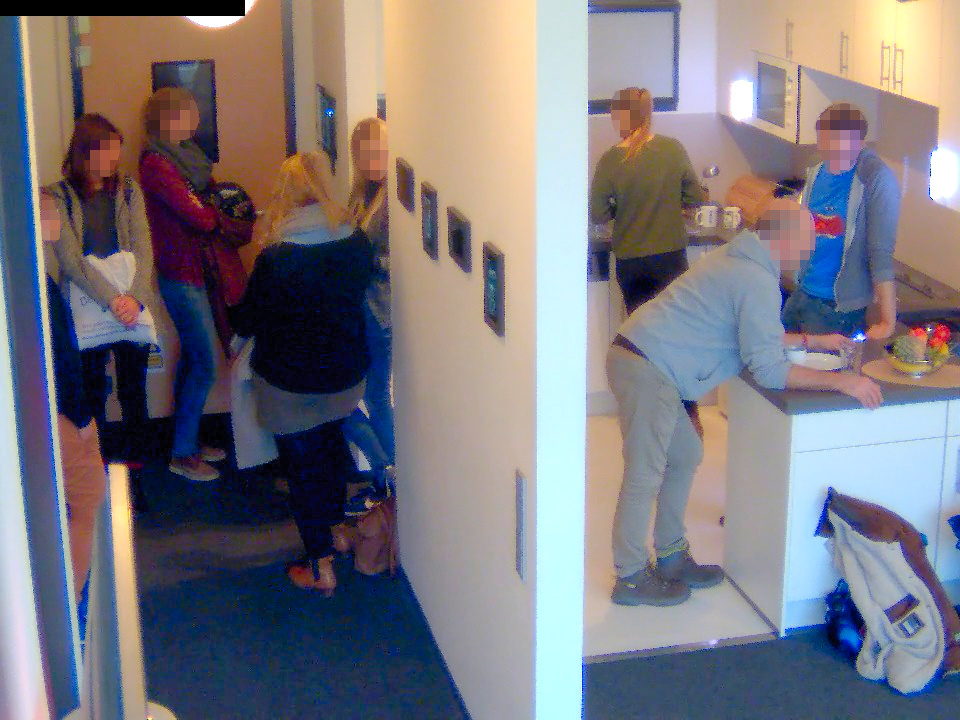
\includegraphics[width=\textwidth]{study-group-shot-cam3}
    \end{column}
    \begin{column}{.5\textwidth}
    \begin{itemize}[label=-]
      \item<1->[] Demonstration Scenario
      \item<1->[\(\rightarrow\)] Human-Agent Conversational Goups
      \item<2-> 10 Guests (8w, 2m) 
      \item<2->[\(\rightarrow\)] Open, Dynamic Interaction
     % \item<3-> Present the Apartment (\SI{20}{min})
     % \item<4-> Free Interaction (\SI{37}{min})
      \item<3->[] \textcolor{mygreen}{New Corpus}
      \item<3-> \SI{57}{min} Video, Audio, IPC
    \end{itemize}
  \end{column}
  \end{columns}
  \vspace{10pt}
  \pnote{25-14}
\end{frame}
\begin{frame}{Person Tracking \& Ground Truth Annotation}
  \begin{columns}[T] % align columns
    \begin{column}{.5\textwidth}
     \centering
      \onslide<1->{
        \resizebox{.9\textwidth}{!}{%
          \def\svgwidth{1.8\textwidth}
          \input{generated/study-group-shots-openpose.pdf_tex}
      }}
  \end{column}%
  \hspace{-.05\textwidth}
    \begin{column}{.55\textwidth}
      \onslide<2->{
      \resizebox{\textwidth}{!}{%
        \def\svgwidth{1.5\textwidth}
        \input{generated/csra_map_annotations.pdf_tex}
        }
      }
   \end{column}%
  \end{columns}
  \vspace{5pt}
  \begin{columns}[T] % align columns
    \begin{column}{.5\textwidth}
      \onslide<1->{\footnotesize
      \begin{itemize}[label=-]
        \item[] Person Poses
        \item OpenPose + Apartment Tracking
      \end{itemize}
      }
   \end{column}%
    \begin{column}{.5\textwidth}
      \onslide<2->{\footnotesize
      \begin{itemize}[label=-]
        \item[]Ground Truth Annotation
        \item 2D Poses of Agents/Participants
        \item Agent's Conversational Groups
        \item Conversational Role of Each Participant
      \end{itemize}
      }
   \end{column}%
  \end{columns}
  \pnote{25-14}
\end{frame}
\begin{frame}{Best Assignment of Agents to Groups}
    \newcommand{\ffmcostd}{\vspace{-182.3pt}}
    {
      \centering
      %\(\text{Assignment Cost}\bcite{Setti2015}\onslide<3->{ = \text{Distance Cost}}\onslide<4->{ + \text{Visibility Cost}}\onslide<5->{ + \text{MDL Prior}}\)\\
      \(\text{Assignment Cost}\onslide<3->{ = \text{Distance Cost}}\onslide<4->{ + \text{Visibility Cost}}\onslide<5->{ + \text{MDL Prior}}\)\\
    }
    \vspace{10pt}
    \onslide<1->{
      \def\svgwidth{1.\textwidth}
      \input{generated/fformation-costs-layer1.pdf_tex}
    }
    \ffmcostd
    \onslide<2->{
      \def\svgwidth{1.\textwidth}
      \input{generated/fformation-costs-layer6.pdf_tex}
    }
    \ffmcostd
    \onslide<3->{
      \def\svgwidth{1.\textwidth}
      \input{generated/fformation-costs-layer3.pdf_tex}
    }
    \ffmcostd
    \onslide<4->{
      \def\svgwidth{1.\textwidth}
      \input{generated/fformation-costs-layer4.pdf_tex}
    }
    \vspace{-10pt}
  \pnote{25-14}
\end{frame}
\begin{frame}{Evaluating F-Formation Detection for HAI}
  \begin{columns}[T] % align columns
    \begin{column}{.55\textwidth}
    \resizebox{1.\textwidth}{!}{%
      \begin{tikzpicture}
        \action<1->{\node (a) at (0,0)
        {
          \resizebox{1.\textwidth}{!}{%
            \scriptsize
            % Created by tikzDevice version 0.12
% !TEX encoding = UTF-8 Unicode
\begin{tikzpicture}[x=1pt,y=1pt]
\definecolor{fillColor}{RGB}{255,255,255}
\path[use as bounding box,fill=fillColor,fill opacity=0.00] (0,0) rectangle (398.34,369.26);
\begin{scope}
\path[clip] (  0.00,  0.00) rectangle (398.34,369.26);
\definecolor{drawColor}{RGB}{255,255,255}
\definecolor{fillColor}{gray}{0.98}

\path[draw=drawColor,line width= 0.6pt,line join=round,line cap=round,fill=fillColor] (  0.00,  0.00) rectangle (398.34,369.26);
\end{scope}
\begin{scope}
\path[clip] ( 34.81, 56.96) rectangle (211.07,347.51);
\definecolor{fillColor}{gray}{0.92}

\path[fill=fillColor] ( 34.81, 56.96) rectangle (211.07,347.51);
\definecolor{drawColor}{RGB}{255,255,255}

\path[draw=drawColor,line width= 0.3pt,line join=round] ( 34.81, 83.38) --
	(211.07, 83.38);

\path[draw=drawColor,line width= 0.3pt,line join=round] ( 34.81,109.79) --
	(211.07,109.79);

\path[draw=drawColor,line width= 0.3pt,line join=round] ( 34.81,136.20) --
	(211.07,136.20);

\path[draw=drawColor,line width= 0.3pt,line join=round] ( 34.81,162.62) --
	(211.07,162.62);

\path[draw=drawColor,line width= 0.3pt,line join=round] ( 34.81,189.03) --
	(211.07,189.03);

\path[draw=drawColor,line width= 0.3pt,line join=round] ( 34.81,215.44) --
	(211.07,215.44);

\path[draw=drawColor,line width= 0.3pt,line join=round] ( 34.81,241.85) --
	(211.07,241.85);

\path[draw=drawColor,line width= 0.3pt,line join=round] ( 34.81,268.27) --
	(211.07,268.27);

\path[draw=drawColor,line width= 0.3pt,line join=round] ( 34.81,294.68) --
	(211.07,294.68);

\path[draw=drawColor,line width= 0.3pt,line join=round] ( 34.81,321.09) --
	(211.07,321.09);

\path[draw=drawColor,line width= 0.3pt,line join=round] ( 58.85, 56.96) --
	( 58.85,347.51);

\path[draw=drawColor,line width= 0.3pt,line join=round] ( 74.87, 56.96) --
	( 74.87,347.51);

\path[draw=drawColor,line width= 0.3pt,line join=round] ( 90.90, 56.96) --
	( 90.90,347.51);

\path[draw=drawColor,line width= 0.3pt,line join=round] (106.93, 56.96) --
	(106.93,347.51);

\path[draw=drawColor,line width= 0.3pt,line join=round] (122.96, 56.96) --
	(122.96,347.51);

\path[draw=drawColor,line width= 0.3pt,line join=round] (155.01, 56.96) --
	(155.01,347.51);

\path[draw=drawColor,line width= 0.3pt,line join=round] (187.06, 56.96) --
	(187.06,347.51);

\path[draw=drawColor,line width= 0.6pt,line join=round] ( 34.81, 70.17) --
	(211.07, 70.17);

\path[draw=drawColor,line width= 0.6pt,line join=round] ( 34.81, 96.58) --
	(211.07, 96.58);

\path[draw=drawColor,line width= 0.6pt,line join=round] ( 34.81,123.00) --
	(211.07,123.00);

\path[draw=drawColor,line width= 0.6pt,line join=round] ( 34.81,149.41) --
	(211.07,149.41);

\path[draw=drawColor,line width= 0.6pt,line join=round] ( 34.81,175.82) --
	(211.07,175.82);

\path[draw=drawColor,line width= 0.6pt,line join=round] ( 34.81,202.24) --
	(211.07,202.24);

\path[draw=drawColor,line width= 0.6pt,line join=round] ( 34.81,228.65) --
	(211.07,228.65);

\path[draw=drawColor,line width= 0.6pt,line join=round] ( 34.81,255.06) --
	(211.07,255.06);

\path[draw=drawColor,line width= 0.6pt,line join=round] ( 34.81,281.47) --
	(211.07,281.47);

\path[draw=drawColor,line width= 0.6pt,line join=round] ( 34.81,307.89) --
	(211.07,307.89);

\path[draw=drawColor,line width= 0.6pt,line join=round] ( 34.81,334.30) --
	(211.07,334.30);

\path[draw=drawColor,line width= 0.6pt,line join=round] ( 42.82, 56.96) --
	( 42.82,347.51);

\path[draw=drawColor,line width= 0.6pt,line join=round] ( 74.87, 56.96) --
	( 74.87,347.51);

\path[draw=drawColor,line width= 0.6pt,line join=round] (106.93, 56.96) --
	(106.93,347.51);

\path[draw=drawColor,line width= 0.6pt,line join=round] (138.98, 56.96) --
	(138.98,347.51);

\path[draw=drawColor,line width= 0.6pt,line join=round] (171.04, 56.96) --
	(171.04,347.51);

\path[draw=drawColor,line width= 0.6pt,line join=round] (203.09, 56.96) --
	(203.09,347.51);
\definecolor{drawColor}{RGB}{77,175,74}

\path[draw=drawColor,line width= 1.1pt,line join=round] ( 42.82,281.09) --
	( 96.24,276.89) --
	(122.96,270.31) --
	(138.98,256.47) --
	(149.67,256.42) --
	(157.30,256.42) --
	(163.02,255.48) --
	(167.48,255.48) --
	(171.04,246.62) --
	(173.95,246.45) --
	(176.38,246.45) --
	(203.06,246.45);

\path[draw=drawColor,line width= 1.1pt,dash pattern=on 2pt off 2pt ,line join=round] ( 42.82,263.35) --
	( 96.24,252.82) --
	(122.96,225.19) --
	(138.98,218.78) --
	(149.67,218.17) --
	(157.30,218.17) --
	(163.02,213.96) --
	(167.48,213.96) --
	(171.04,211.68) --
	(173.95,211.33) --
	(176.38,211.33) --
	(203.06,211.33);
\end{scope}
\begin{scope}
\path[clip] (216.57, 56.96) rectangle (392.84,347.51);
\definecolor{fillColor}{gray}{0.92}

\path[fill=fillColor] (216.57, 56.96) rectangle (392.84,347.51);
\definecolor{drawColor}{RGB}{255,255,255}

\path[draw=drawColor,line width= 0.3pt,line join=round] (216.57, 83.38) --
	(392.84, 83.38);

\path[draw=drawColor,line width= 0.3pt,line join=round] (216.57,109.79) --
	(392.84,109.79);

\path[draw=drawColor,line width= 0.3pt,line join=round] (216.57,136.20) --
	(392.84,136.20);

\path[draw=drawColor,line width= 0.3pt,line join=round] (216.57,162.62) --
	(392.84,162.62);

\path[draw=drawColor,line width= 0.3pt,line join=round] (216.57,189.03) --
	(392.84,189.03);

\path[draw=drawColor,line width= 0.3pt,line join=round] (216.57,215.44) --
	(392.84,215.44);

\path[draw=drawColor,line width= 0.3pt,line join=round] (216.57,241.85) --
	(392.84,241.85);

\path[draw=drawColor,line width= 0.3pt,line join=round] (216.57,268.27) --
	(392.84,268.27);

\path[draw=drawColor,line width= 0.3pt,line join=round] (216.57,294.68) --
	(392.84,294.68);

\path[draw=drawColor,line width= 0.3pt,line join=round] (216.57,321.09) --
	(392.84,321.09);

\path[draw=drawColor,line width= 0.3pt,line join=round] (240.61, 56.96) --
	(240.61,347.51);

\path[draw=drawColor,line width= 0.3pt,line join=round] (256.64, 56.96) --
	(256.64,347.51);

\path[draw=drawColor,line width= 0.3pt,line join=round] (272.67, 56.96) --
	(272.67,347.51);

\path[draw=drawColor,line width= 0.3pt,line join=round] (288.69, 56.96) --
	(288.69,347.51);

\path[draw=drawColor,line width= 0.3pt,line join=round] (304.72, 56.96) --
	(304.72,347.51);

\path[draw=drawColor,line width= 0.3pt,line join=round] (336.78, 56.96) --
	(336.78,347.51);

\path[draw=drawColor,line width= 0.3pt,line join=round] (368.83, 56.96) --
	(368.83,347.51);

\path[draw=drawColor,line width= 0.6pt,line join=round] (216.57, 70.17) --
	(392.84, 70.17);

\path[draw=drawColor,line width= 0.6pt,line join=round] (216.57, 96.58) --
	(392.84, 96.58);

\path[draw=drawColor,line width= 0.6pt,line join=round] (216.57,123.00) --
	(392.84,123.00);

\path[draw=drawColor,line width= 0.6pt,line join=round] (216.57,149.41) --
	(392.84,149.41);

\path[draw=drawColor,line width= 0.6pt,line join=round] (216.57,175.82) --
	(392.84,175.82);

\path[draw=drawColor,line width= 0.6pt,line join=round] (216.57,202.24) --
	(392.84,202.24);

\path[draw=drawColor,line width= 0.6pt,line join=round] (216.57,228.65) --
	(392.84,228.65);

\path[draw=drawColor,line width= 0.6pt,line join=round] (216.57,255.06) --
	(392.84,255.06);

\path[draw=drawColor,line width= 0.6pt,line join=round] (216.57,281.47) --
	(392.84,281.47);

\path[draw=drawColor,line width= 0.6pt,line join=round] (216.57,307.89) --
	(392.84,307.89);

\path[draw=drawColor,line width= 0.6pt,line join=round] (216.57,334.30) --
	(392.84,334.30);

\path[draw=drawColor,line width= 0.6pt,line join=round] (224.58, 56.96) --
	(224.58,347.51);

\path[draw=drawColor,line width= 0.6pt,line join=round] (256.64, 56.96) --
	(256.64,347.51);

\path[draw=drawColor,line width= 0.6pt,line join=round] (288.69, 56.96) --
	(288.69,347.51);

\path[draw=drawColor,line width= 0.6pt,line join=round] (320.75, 56.96) --
	(320.75,347.51);

\path[draw=drawColor,line width= 0.6pt,line join=round] (352.80, 56.96) --
	(352.80,347.51);

\path[draw=drawColor,line width= 0.6pt,line join=round] (384.86, 56.96) --
	(384.86,347.51);
\definecolor{drawColor}{RGB}{77,175,74}

\path[draw=drawColor,line width= 1.1pt,line join=round] (224.58,229.99) --
	(278.01,227.94) --
	(304.72,220.91) --
	(320.75,214.02) --
	(331.43,213.76) --
	(339.07,213.76) --
	(344.79,213.63) --
	(349.24,213.63) --
	(352.80,213.33) --
	(355.72,213.17) --
	(358.15,213.17) --
	(384.83,213.17);

\path[draw=drawColor,line width= 1.1pt,dash pattern=on 2pt off 2pt ,line join=round] (224.58,191.24) --
	(278.01,182.38) --
	(304.72,143.96) --
	(320.75,141.36) --
	(331.43,140.83) --
	(339.07,140.83) --
	(344.79,140.69) --
	(349.24,140.69) --
	(352.80,131.47) --
	(355.72,130.62) --
	(358.15,130.62) --
	(384.83,130.62);
\end{scope}
\begin{scope}
\path[clip] ( 34.81,347.51) rectangle (211.07,363.76);
\definecolor{fillColor}{gray}{0.85}

\path[fill=fillColor] ( 34.81,347.51) rectangle (211.07,363.76);
\definecolor{drawColor}{gray}{0.10}

\node[text=drawColor,anchor=base,inner sep=0pt, outer sep=0pt, scale=  0.80] at (122.94,352.88) {Flobi Assistance};
\end{scope}
\begin{scope}
\path[clip] (216.57,347.51) rectangle (392.84,363.76);
\definecolor{fillColor}{gray}{0.85}

\path[fill=fillColor] (216.57,347.51) rectangle (392.84,363.76);
\definecolor{drawColor}{gray}{0.10}

\node[text=drawColor,anchor=base,inner sep=0pt, outer sep=0pt, scale=  0.80] at (304.71,352.88) {Flobi Entrance};
\end{scope}
\begin{scope}
\path[clip] (  0.00,  0.00) rectangle (398.34,369.26);
\definecolor{drawColor}{gray}{0.20}

\path[draw=drawColor,line width= 0.6pt,line join=round] ( 42.82, 54.21) --
	( 42.82, 56.96);

\path[draw=drawColor,line width= 0.6pt,line join=round] ( 74.87, 54.21) --
	( 74.87, 56.96);

\path[draw=drawColor,line width= 0.6pt,line join=round] (106.93, 54.21) --
	(106.93, 56.96);

\path[draw=drawColor,line width= 0.6pt,line join=round] (138.98, 54.21) --
	(138.98, 56.96);

\path[draw=drawColor,line width= 0.6pt,line join=round] (171.04, 54.21) --
	(171.04, 56.96);

\path[draw=drawColor,line width= 0.6pt,line join=round] (203.09, 54.21) --
	(203.09, 56.96);
\end{scope}
\begin{scope}
\path[clip] (  0.00,  0.00) rectangle (398.34,369.26);
\definecolor{drawColor}{RGB}{0,0,0}

\node[text=drawColor,rotate= 60.00,anchor=base,inner sep=0pt, outer sep=0pt, scale=  1.00] at ( 48.78, 48.57) {0.5};

\node[text=drawColor,rotate= 60.00,anchor=base,inner sep=0pt, outer sep=0pt, scale=  1.00] at ( 80.84, 48.57) {0.6};

\node[text=drawColor,rotate= 60.00,anchor=base,inner sep=0pt, outer sep=0pt, scale=  1.00] at (112.89, 48.57) {0.7};

\node[text=drawColor,rotate= 60.00,anchor=base,inner sep=0pt, outer sep=0pt, scale=  1.00] at (144.95, 48.57) {0.8};

\node[text=drawColor,rotate= 60.00,anchor=base,inner sep=0pt, outer sep=0pt, scale=  1.00] at (177.00, 48.57) {0.9};

\node[text=drawColor,rotate= 60.00,anchor=base,inner sep=0pt, outer sep=0pt, scale=  1.00] at (209.06, 48.57) {1.0};
\end{scope}
\begin{scope}
\path[clip] (  0.00,  0.00) rectangle (398.34,369.26);
\definecolor{drawColor}{gray}{0.20}

\path[draw=drawColor,line width= 0.6pt,line join=round] (224.58, 54.21) --
	(224.58, 56.96);

\path[draw=drawColor,line width= 0.6pt,line join=round] (256.64, 54.21) --
	(256.64, 56.96);

\path[draw=drawColor,line width= 0.6pt,line join=round] (288.69, 54.21) --
	(288.69, 56.96);

\path[draw=drawColor,line width= 0.6pt,line join=round] (320.75, 54.21) --
	(320.75, 56.96);

\path[draw=drawColor,line width= 0.6pt,line join=round] (352.80, 54.21) --
	(352.80, 56.96);

\path[draw=drawColor,line width= 0.6pt,line join=round] (384.86, 54.21) --
	(384.86, 56.96);
\end{scope}
\begin{scope}
\path[clip] (  0.00,  0.00) rectangle (398.34,369.26);
\definecolor{drawColor}{RGB}{0,0,0}

\node[text=drawColor,rotate= 60.00,anchor=base,inner sep=0pt, outer sep=0pt, scale=  1.00] at (230.55, 48.57) {0.5};

\node[text=drawColor,rotate= 60.00,anchor=base,inner sep=0pt, outer sep=0pt, scale=  1.00] at (262.60, 48.57) {0.6};

\node[text=drawColor,rotate= 60.00,anchor=base,inner sep=0pt, outer sep=0pt, scale=  1.00] at (294.66, 48.57) {0.7};

\node[text=drawColor,rotate= 60.00,anchor=base,inner sep=0pt, outer sep=0pt, scale=  1.00] at (326.71, 48.57) {0.8};

\node[text=drawColor,rotate= 60.00,anchor=base,inner sep=0pt, outer sep=0pt, scale=  1.00] at (358.77, 48.57) {0.9};

\node[text=drawColor,rotate= 60.00,anchor=base,inner sep=0pt, outer sep=0pt, scale=  1.00] at (390.82, 48.57) {1.0};
\end{scope}
\begin{scope}
\path[clip] (  0.00,  0.00) rectangle (398.34,369.26);
\definecolor{drawColor}{RGB}{0,0,0}

\node[text=drawColor,anchor=base east,inner sep=0pt, outer sep=0pt, scale=  1.00] at ( 29.86, 66.73) {0.0};

\node[text=drawColor,anchor=base east,inner sep=0pt, outer sep=0pt, scale=  1.00] at ( 29.86, 93.14) {0.1};

\node[text=drawColor,anchor=base east,inner sep=0pt, outer sep=0pt, scale=  1.00] at ( 29.86,119.55) {0.2};

\node[text=drawColor,anchor=base east,inner sep=0pt, outer sep=0pt, scale=  1.00] at ( 29.86,145.97) {0.3};

\node[text=drawColor,anchor=base east,inner sep=0pt, outer sep=0pt, scale=  1.00] at ( 29.86,172.38) {0.4};

\node[text=drawColor,anchor=base east,inner sep=0pt, outer sep=0pt, scale=  1.00] at ( 29.86,198.79) {0.5};

\node[text=drawColor,anchor=base east,inner sep=0pt, outer sep=0pt, scale=  1.00] at ( 29.86,225.20) {0.6};

\node[text=drawColor,anchor=base east,inner sep=0pt, outer sep=0pt, scale=  1.00] at ( 29.86,251.62) {0.7};

\node[text=drawColor,anchor=base east,inner sep=0pt, outer sep=0pt, scale=  1.00] at ( 29.86,278.03) {0.8};

\node[text=drawColor,anchor=base east,inner sep=0pt, outer sep=0pt, scale=  1.00] at ( 29.86,304.44) {0.9};

\node[text=drawColor,anchor=base east,inner sep=0pt, outer sep=0pt, scale=  1.00] at ( 29.86,330.86) {1.0};
\end{scope}
\begin{scope}
\path[clip] (  0.00,  0.00) rectangle (398.34,369.26);
\definecolor{drawColor}{gray}{0.20}

\path[draw=drawColor,line width= 0.6pt,line join=round] ( 32.06, 70.17) --
	( 34.81, 70.17);

\path[draw=drawColor,line width= 0.6pt,line join=round] ( 32.06, 96.58) --
	( 34.81, 96.58);

\path[draw=drawColor,line width= 0.6pt,line join=round] ( 32.06,123.00) --
	( 34.81,123.00);

\path[draw=drawColor,line width= 0.6pt,line join=round] ( 32.06,149.41) --
	( 34.81,149.41);

\path[draw=drawColor,line width= 0.6pt,line join=round] ( 32.06,175.82) --
	( 34.81,175.82);

\path[draw=drawColor,line width= 0.6pt,line join=round] ( 32.06,202.24) --
	( 34.81,202.24);

\path[draw=drawColor,line width= 0.6pt,line join=round] ( 32.06,228.65) --
	( 34.81,228.65);

\path[draw=drawColor,line width= 0.6pt,line join=round] ( 32.06,255.06) --
	( 34.81,255.06);

\path[draw=drawColor,line width= 0.6pt,line join=round] ( 32.06,281.47) --
	( 34.81,281.47);

\path[draw=drawColor,line width= 0.6pt,line join=round] ( 32.06,307.89) --
	( 34.81,307.89);

\path[draw=drawColor,line width= 0.6pt,line join=round] ( 32.06,334.30) --
	( 34.81,334.30);
\end{scope}
\begin{scope}
\path[clip] (  0.00,  0.00) rectangle (398.34,369.26);
\definecolor{drawColor}{RGB}{0,0,0}

\node[text=drawColor,anchor=base,inner sep=0pt, outer sep=0pt, scale=  1.00] at (213.82, 26.90) {Tolerance Threshold};
\end{scope}
\begin{scope}
\path[clip] (  0.00,  0.00) rectangle (398.34,369.26);
\definecolor{drawColor}{RGB}{0,0,0}

\node[text=drawColor,rotate= 90.00,anchor=base,inner sep=0pt, outer sep=0pt, scale=  1.00] at ( 12.39,202.24) {F1};
\end{scope}
\begin{scope}
\path[clip] (  0.00,  0.00) rectangle (398.34,369.26);
\definecolor{fillColor}{RGB}{255,255,255}

\path[fill=fillColor] (131.24,  5.50) rectangle (296.40, 23.95);
\end{scope}
\begin{scope}
\path[clip] (  0.00,  0.00) rectangle (398.34,369.26);
\definecolor{drawColor}{RGB}{0,0,0}

\node[text=drawColor,anchor=base west,inner sep=0pt, outer sep=0pt, scale=  1.00] at (133.24, 11.28) {Input};
\end{scope}
\begin{scope}
\path[clip] (  0.00,  0.00) rectangle (398.34,369.26);
\definecolor{drawColor}{RGB}{255,255,255}
\definecolor{fillColor}{gray}{0.95}

\path[draw=drawColor,line width= 0.6pt,line join=round,line cap=round,fill=fillColor] (162.40,  7.50) rectangle (176.86, 21.95);
\end{scope}
\begin{scope}
\path[clip] (  0.00,  0.00) rectangle (398.34,369.26);
\definecolor{drawColor}{RGB}{77,175,74}

\path[draw=drawColor,line width= 1.1pt,line join=round] (163.85, 14.73) -- (175.41, 14.73);
\end{scope}
\begin{scope}
\path[clip] (  0.00,  0.00) rectangle (398.34,369.26);
\definecolor{drawColor}{RGB}{255,255,255}
\definecolor{fillColor}{gray}{0.95}

\path[draw=drawColor,line width= 0.6pt,line join=round,line cap=round,fill=fillColor] (233.96,  7.50) rectangle (248.41, 21.95);
\end{scope}
\begin{scope}
\path[clip] (  0.00,  0.00) rectangle (398.34,369.26);
\definecolor{drawColor}{RGB}{77,175,74}

\path[draw=drawColor,line width= 1.1pt,dash pattern=on 2pt off 2pt ,line join=round] (235.40, 14.73) -- (246.97, 14.73);
\end{scope}
\begin{scope}
\path[clip] (  0.00,  0.00) rectangle (398.34,369.26);
\definecolor{drawColor}{RGB}{0,0,0}

\node[text=drawColor,anchor=base west,inner sep=0pt, outer sep=0pt, scale=  0.80] at (181.86, 11.97) {Annotated};
\end{scope}
\begin{scope}
\path[clip] (  0.00,  0.00) rectangle (398.34,369.26);
\definecolor{drawColor}{RGB}{0,0,0}

\node[text=drawColor,anchor=base west,inner sep=0pt, outer sep=0pt, scale=  0.80] at (253.41, 11.97) {Detected};
\end{scope}
\end{tikzpicture}

          }
        };}
        \action<1>{\filldraw [fill=bgcolorframe, draw=bgcolorframe] (-90pt,-58pt) rectangle (105pt,88pt);}
      \end{tikzpicture}
    }
    \end{column}
    \hspace{-20pt}
    \begin{column}{.52\textwidth}
      \footnotesize
      \vspace{30pt}
      \begin{itemize}
        \item[-]<1-> Graph-Cuts with \(\text{MDL} = 4500\), \(\text{Stride} = 50\)
        \item[-]<1-> \(F_1\) for Tolerance Threshold \([0.5,1]\)
        \item[-]<2-> Pose detection errors reduce group detection quality
        \item[-]<3-> Overall worse Performance for Flobi Entrance
        \item[-]<4-> Good results given the complexity
        \item[\textcolor{mygreen}{\faCheckCircle}]<5-> \emph{F-Formations known from HHI can be used to detect conversational groups of people and artificial agents.}
      \end{itemize}
    \end{column}
  \end{columns}
  \pnote{25-14 (16/17 ist eine gute zeit)}
\end{frame}
\begin{frame}{In/Out of Group Distinction}
  \vspace{20pt}
  \begin{columns}[T] % align columns
    \begin{column}{.3\textwidth}
      \vspace{3pt}
      \centering
      \onslide<1->{\resizebox{\textwidth}{!}{%
      \def\svgwidth{1.5\textwidth}
        \input{generated/conversational_group_defence.pdf_tex}
      }}
    \end{column}%
    \begin{column}{.3\textwidth}
      \onslide<1->{
        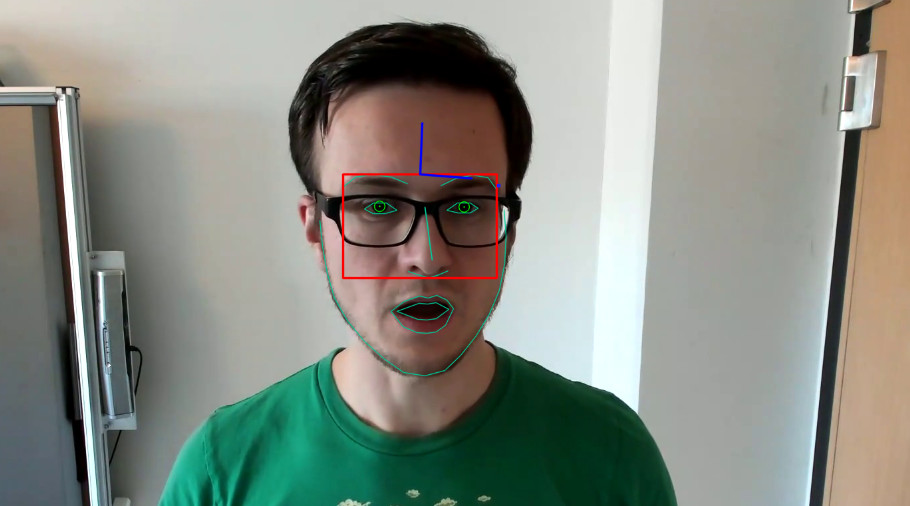
\includegraphics[trim={3.5cm .8cm 6cm 0}, clip, width=\textwidth]{meka-face-speaking}
      }
   \end{column}%
   \begin{column}{.3\textwidth}
      \onslide<1->{
        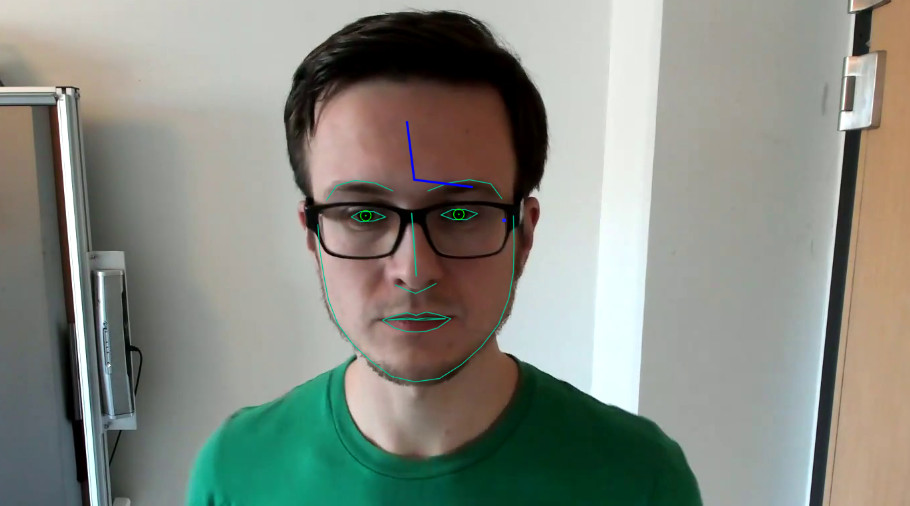
\includegraphics[trim={4cm .8cm 5.5cm 0}, clip, width=\textwidth]{meka-face-nonspeaking}
      }
   \end{column}%
  \end{columns}
  \begin{columns}[T] % align columns
    \begin{column}{.3\textwidth}
      \onslide<2->{
      \centering
        Costs from F-Formation\\\textcolor{mygreen}{F-Formation}
      }
    \end{column}%
    \begin{column}{.3\textwidth}
      \onslide<3->{
      \centering
        Gaze Angle\\\textcolor{myblue}{Gaze}
      }
    \end{column}%
    \begin{column}{.3\textwidth}
      \centering
      \onslide<4->{
        Face Size\\\textcolor{myred}{Face}
      }
    \end{column}%
  \end{columns}
  \pnote{25-14}
\end{frame}
\begin{frame}{In/Out of Group Distinction}
  \begin{columns}[T] % align columns
    \begin{column}{.65\textwidth}
      \vspace{30pt}
      \resizebox{1.\textwidth}{!}{%
        \scriptsize
        %% Created by tikzDevice version 0.12
% !TEX encoding = UTF-8 Unicode
\begin{tikzpicture}[x=1pt,y=1pt]
\definecolor{fillColor}{RGB}{255,255,255}
\path[use as bounding box,fill=fillColor,fill opacity=0.00] (0,0) rectangle (398.34,246.17);
\begin{scope}
\path[clip] (  0.00,  0.00) rectangle (398.34,246.17);
\definecolor{drawColor}{RGB}{255,255,255}
\definecolor{fillColor}{gray}{0.98}

\path[draw=drawColor,line width= 0.6pt,line join=round,line cap=round,fill=fillColor] (  0.00,  0.00) rectangle (398.34,246.17);
\end{scope}
\begin{scope}
\path[clip] ( 39.80, 30.86) rectangle (294.26,240.67);
\definecolor{fillColor}{gray}{0.92}

\path[fill=fillColor] ( 39.80, 30.86) rectangle (294.26,240.67);
\definecolor{drawColor}{RGB}{255,255,255}

\path[draw=drawColor,line width= 0.3pt,line join=round] ( 39.80, 64.22) --
	(294.26, 64.22);

\path[draw=drawColor,line width= 0.3pt,line join=round] ( 39.80,111.91) --
	(294.26,111.91);

\path[draw=drawColor,line width= 0.3pt,line join=round] ( 39.80,159.60) --
	(294.26,159.60);

\path[draw=drawColor,line width= 0.3pt,line join=round] ( 39.80,207.29) --
	(294.26,207.29);

\path[draw=drawColor,line width= 0.3pt,line join=round] ( 80.29, 30.86) --
	( 80.29,240.67);

\path[draw=drawColor,line width= 0.3pt,line join=round] (138.12, 30.86) --
	(138.12,240.67);

\path[draw=drawColor,line width= 0.3pt,line join=round] (195.95, 30.86) --
	(195.95,240.67);

\path[draw=drawColor,line width= 0.3pt,line join=round] (253.78, 30.86) --
	(253.78,240.67);

\path[draw=drawColor,line width= 0.6pt,line join=round] ( 39.80, 40.37) --
	(294.26, 40.37);

\path[draw=drawColor,line width= 0.6pt,line join=round] ( 39.80, 88.06) --
	(294.26, 88.06);

\path[draw=drawColor,line width= 0.6pt,line join=round] ( 39.80,135.75) --
	(294.26,135.75);

\path[draw=drawColor,line width= 0.6pt,line join=round] ( 39.80,183.44) --
	(294.26,183.44);

\path[draw=drawColor,line width= 0.6pt,line join=round] ( 39.80,231.14) --
	(294.26,231.14);

\path[draw=drawColor,line width= 0.6pt,line join=round] ( 51.37, 30.86) --
	( 51.37,240.67);

\path[draw=drawColor,line width= 0.6pt,line join=round] (109.20, 30.86) --
	(109.20,240.67);

\path[draw=drawColor,line width= 0.6pt,line join=round] (167.03, 30.86) --
	(167.03,240.67);

\path[draw=drawColor,line width= 0.6pt,line join=round] (224.87, 30.86) --
	(224.87,240.67);

\path[draw=drawColor,line width= 0.6pt,line join=round] (282.70, 30.86) --
	(282.70,240.67);
\definecolor{fillColor}{RGB}{89,89,89}

\path[fill=fillColor,fill opacity=0.30] ( 86.07, 68.99) rectangle (248.00,154.83);
\definecolor{drawColor}{RGB}{0,0,0}

\node[text=drawColor,anchor=base,inner sep=0pt, outer sep=0pt, scale=  1.10] at (167.03,108.11) {\footnotesize{AUC}};
\definecolor{drawColor}{RGB}{228,26,28}

\path[draw=drawColor,line width= 1.1pt,line join=round] ( 51.37, 46.70) --
	( 51.37, 44.82) --
	( 51.37, 44.76) --
	( 51.37, 40.65) --
	( 51.42, 59.92) --
	( 51.42, 59.91) --
	( 51.42, 59.90) --
	( 51.43, 61.49) --
	( 51.67, 72.23) --
	( 51.86, 84.25) --
	( 51.86, 84.22) --
	( 51.86, 84.21) --
	( 51.86, 84.19) --
	( 52.40, 89.75) --
	( 53.01,108.51) --
	( 53.56,123.92) --
	( 53.57,124.33) --
	( 53.58,124.47) --
	( 54.31,134.44) --
	( 55.56,152.16) --
	( 56.18,157.35) --
	( 56.23,157.44) --
	( 56.34,157.64) --
	( 56.77,160.52) --
	( 57.64,167.74) --
	( 58.42,172.25) --
	( 58.50,172.50) --
	( 61.90,191.39) --
	(282.70,231.14);

\path[draw=drawColor,line width= 1.1pt,dash pattern=on 2pt off 2pt ,line join=round] ( 51.37, 42.80) --
	( 51.37, 41.27) --
	( 51.37, 40.98) --
	( 51.37, 40.57) --
	( 51.38, 50.87) --
	( 51.38, 50.84) --
	( 51.38, 50.77) --
	( 51.38, 49.46) --
	( 51.38, 47.72) --
	( 51.38, 43.78) --
	( 51.38, 52.92) --
	( 51.42, 52.92) --
	( 51.57, 65.98) --
	( 51.75, 68.28) --
	( 51.75, 67.90) --
	( 52.02, 76.84) --
	( 52.03,132.44) --
	( 52.29,132.87) --
	( 52.78,133.46) --
	( 52.98,133.51) --
	( 53.10,133.51) --
	( 53.18,135.05) --
	( 53.65,144.11) --
	( 53.97,157.38) --
	( 53.98,157.38) --
	( 54.06,157.38) --
	( 54.84,157.38) --
	( 54.89,157.41) --
	( 54.94,158.40) --
	( 55.09,159.99) --
	( 55.13,163.55) --
	( 55.16,163.55) --
	( 55.22,165.47) --
	( 55.28,168.06) --
	( 55.34,168.29) --
	( 55.46,168.29) --
	( 55.55,168.29) --
	( 55.67,170.95) --
	( 56.16,181.22) --
	( 56.51,185.12) --
	( 56.57,185.17) --
	(282.70,231.14);
\definecolor{drawColor}{RGB}{55,126,184}

\path[draw=drawColor,line width= 1.1pt,line join=round] ( 51.37, 40.40) --
	( 51.38, 40.42) --
	( 51.38, 40.46) --
	( 51.39, 40.48) --
	( 51.39, 40.51) --
	( 51.39, 40.54) --
	( 51.39, 40.56) --
	( 51.39, 40.59) --
	( 51.40, 40.61) --
	( 51.41, 40.63) --
	( 51.41, 40.66) --
	( 51.41, 40.72) --
	( 51.41, 40.75) --
	( 51.41, 40.79) --
	( 51.41, 40.83) --
	( 51.41, 40.86) --
	( 51.41, 40.88) --
	( 51.41, 40.91) --
	( 51.41, 40.94) --
	( 51.41, 40.97) --
	( 51.41, 41.00) --
	( 51.41, 41.03) --
	( 51.41, 41.06) --
	( 51.41, 41.10) --
	( 51.42, 41.12) --
	( 51.42, 41.15) --
	( 51.42, 41.18) --
	( 51.42, 41.22) --
	( 51.43, 41.23) --
	( 51.43, 41.26) --
	( 51.43, 41.29) --
	( 51.44, 41.31) --
	( 51.45, 41.33) --
	( 51.45, 41.37) --
	( 51.45, 41.40) --
	( 51.45, 41.43) --
	( 51.45, 41.46) --
	( 51.45, 41.49) --
	( 51.45, 41.52) --
	( 51.45, 41.56) --
	( 51.45, 41.58) --
	( 51.45, 41.61) --
	( 51.45, 41.63) --
	( 51.45, 41.67) --
	( 51.45, 41.71) --
	( 51.45, 41.75) --
	( 51.45, 41.78) --
	( 51.45, 41.81) --
	( 51.45, 41.85) --
	( 51.45, 41.88) --
	( 51.45, 41.90) --
	( 51.46, 41.92) --
	( 51.46, 41.95) --
	( 51.46, 41.99) --
	( 51.47, 42.00) --
	( 51.47, 42.04) --
	( 51.47, 42.08) --
	( 51.48, 42.11) --
	( 51.48, 42.15) --
	( 51.49, 42.18) --
	( 51.49, 42.21) --
	( 51.49, 42.24) --
	( 51.50, 42.26) --
	( 51.50, 42.29) --
	( 51.50, 42.34) --
	( 51.50, 42.37) --
	( 51.50, 42.40) --
	( 51.50, 42.44) --
	( 51.50, 42.48) --
	( 51.50, 42.51) --
	( 51.50, 42.54) --
	( 51.50, 42.56) --
	( 51.50, 42.59) --
	( 51.50, 42.62) --
	( 51.50, 42.66) --
	( 51.50, 42.70) --
	( 51.51, 42.72) --
	( 51.51, 42.77) --
	( 51.51, 42.80) --
	( 51.51, 42.83) --
	( 51.51, 42.87) --
	( 51.51, 42.91) --
	( 51.53, 42.93) --
	( 51.53, 42.96) --
	( 51.53, 42.99) --
	( 51.53, 43.02) --
	( 51.53, 43.05) --
	( 51.54, 43.07) --
	( 51.54, 43.10) --
	( 51.54, 43.13) --
	( 51.55, 43.16) --
	( 51.55, 43.19) --
	( 51.55, 43.22) --
	( 51.56, 43.24) --
	( 51.56, 43.26) --
	( 51.56, 43.29) --
	( 51.56, 43.33) --
	( 51.56, 43.36) --
	( 51.56, 43.38) --
	( 51.57, 43.41) --
	( 51.57, 43.44) --
	( 51.57, 43.47) --
	( 51.58, 43.49) --
	( 51.59, 43.51) --
	( 51.59, 43.54) --
	( 51.59, 43.57) --
	( 51.59, 43.59) --
	( 51.59, 43.62) --
	( 51.59, 43.65) --
	( 51.59, 43.68) --
	( 51.60, 43.71) --
	( 51.60, 43.74) --
	( 51.60, 43.77) --
	( 51.61, 43.80) --
	( 51.61, 43.83) --
	( 51.62, 43.85) --
	( 51.62, 43.88) --
	( 51.62, 43.91) --
	( 51.62, 43.93) --
	( 51.62, 43.96) --
	( 51.62, 43.99) --
	( 51.63, 44.02) --
	( 51.63, 44.05) --
	( 51.63, 44.08) --
	( 51.63, 44.11) --
	( 51.63, 44.14) --
	( 51.63, 44.17) --
	( 51.64, 44.20) --
	( 51.64, 44.23) --
	( 51.64, 44.27) --
	( 51.64, 44.32) --
	( 51.64, 44.36) --
	( 51.65, 44.38) --
	( 51.65, 44.42) --
	( 51.65, 44.45) --
	( 51.65, 44.49) --
	( 51.65, 44.51) --
	( 51.65, 44.54) --
	( 51.65, 44.57) --
	( 51.65, 44.60) --
	( 51.65, 44.63) --
	( 51.65, 44.66) --
	( 51.65, 44.69) --
	( 51.65, 44.73) --
	( 51.65, 44.77) --
	( 51.65, 44.80) --
	( 51.65, 44.83) --
	( 51.65, 44.87) --
	( 51.65, 44.91) --
	( 51.65, 44.94) --
	( 51.65, 44.96) --
	( 51.65, 44.99) --
	( 51.65, 45.02) --
	( 51.65, 45.05) --
	( 51.66, 45.07) --
	( 51.66, 45.10) --
	( 51.67, 45.12) --
	( 51.67, 45.15) --
	( 51.67, 45.20) --
	( 51.68, 45.22) --
	( 51.68, 45.25) --
	( 51.68, 45.28) --
	( 51.68, 45.29) --
	( 51.68, 45.33) --
	( 51.68, 45.36) --
	( 51.68, 45.40) --
	( 51.70, 45.42) --
	( 51.70, 45.45) --
	( 51.70, 45.48) --
	( 51.70, 45.51) --
	( 51.70, 45.54) --
	( 51.70, 45.58) --
	( 51.70, 45.60) --
	( 51.70, 45.63) --
	( 51.70, 45.65) --
	( 51.70, 45.68) --
	( 51.70, 45.71) --
	( 51.70, 45.74) --
	( 51.71, 45.76) --
	( 51.71, 45.79) --
	( 51.71, 45.82) --
	( 51.71, 45.85) --
	( 51.71, 45.89) --
	( 51.71, 45.93) --
	( 51.71, 45.96) --
	( 51.71, 45.98) --
	( 51.71, 46.01) --
	( 51.71, 46.04) --
	( 51.71, 46.10) --
	( 51.71, 46.13) --
	( 51.71, 46.16) --
	( 51.71, 46.19) --
	( 51.71, 46.22) --
	( 51.71, 46.25) --
	( 51.71, 46.28) --
	( 51.71, 46.31) --
	( 51.72, 46.33) --
	( 51.72, 46.36) --
	( 51.72, 46.40) --
	( 51.72, 46.43) --
	( 51.72, 46.46) --
	( 51.73, 46.48) --
	( 51.73, 46.50) --
	( 51.74, 46.52) --
	( 51.75, 46.54) --
	( 51.76, 46.56) --
	( 51.76, 46.59) --
	( 51.76, 46.62) --
	( 51.76, 46.65) --
	( 51.76, 46.66) --
	( 51.76, 46.72) --
	( 51.76, 46.76) --
	( 51.77, 46.78) --
	( 51.77, 46.81) --
	( 51.77, 46.84) --
	( 51.77, 46.87) --
	( 51.77, 46.90) --
	( 51.77, 46.93) --
	( 51.77, 46.96) --
	( 51.77, 46.99) --
	( 51.77, 47.01) --
	( 51.77, 47.04) --
	( 51.77, 47.07) --
	( 51.77, 47.10) --
	( 51.77, 47.14) --
	( 51.78, 47.16) --
	( 51.78, 47.19) --
	( 51.79, 47.21) --
	( 51.79, 47.24) --
	( 51.79, 47.27) --
	( 51.79, 47.30) --
	( 51.79, 47.33) --
	( 51.79, 47.35) --
	( 51.79, 47.38) --
	( 51.80, 47.40) --
	( 51.80, 47.44) --
	( 51.81, 47.46) --
	( 51.81, 47.49) --
	( 51.81, 47.52) --
	( 51.81, 47.55) --
	( 51.82, 47.57) --
	( 51.82, 47.60) --
	( 51.82, 47.64) --
	( 51.82, 47.67) --
	( 51.82, 47.70) --
	( 51.82, 47.73) --
	( 51.83, 47.75) --
	( 51.83, 47.78) --
	( 51.83, 47.82) --
	( 51.83, 47.86) --
	( 51.83, 47.89) --
	( 51.83, 47.92) --
	( 51.83, 47.95) --
	( 51.83, 47.98) --
	( 51.85, 48.00) --
	( 51.85, 48.02) --
	( 51.85, 48.05) --
	( 51.86, 48.07) --
	( 51.86, 48.10) --
	( 51.87, 48.13) --
	( 51.87, 48.17) --
	( 51.87, 48.20) --
	( 51.87, 48.24) --
	( 51.87, 48.28) --
	( 51.88, 48.30) --
	( 51.88, 48.33) --
	( 51.88, 48.35) --
	( 51.88, 48.38) --
	( 51.88, 48.41) --
	( 51.88, 48.44) --
	( 51.89, 48.46) --
	( 51.89, 48.51) --
	( 51.89, 48.54) --
	( 51.89, 48.58) --
	( 51.89, 48.61) --
	( 51.89, 48.64) --
	( 51.89, 48.68) --
	( 51.89, 48.71) --
	( 51.90, 48.73) --
	( 51.90, 48.77) --
	( 51.90, 48.79) --
	( 51.91, 48.81) --
	( 51.91, 48.85) --
	( 51.91, 48.88) --
	( 51.91, 48.91) --
	( 51.91, 48.95) --
	( 51.92, 48.97) --
	( 51.92, 49.00) --
	( 51.92, 49.02) --
	( 51.92, 49.05) --
	( 51.93, 49.06) --
	( 51.93, 49.09) --
	( 51.93, 49.12) --
	( 51.94, 49.14) --
	( 51.95, 49.16) --
	( 51.95, 49.19) --
	( 51.95, 49.22) --
	( 51.95, 49.25) --
	( 51.96, 49.28) --
	( 51.96, 49.32) --
	( 51.96, 49.36) --
	( 51.96, 49.38) --
	( 51.97, 49.41) --
	( 51.97, 49.44) --
	( 51.97, 49.48) --
	( 51.97, 49.51) --
	( 51.97, 49.55) --
	( 51.97, 49.58) --
	( 51.97, 49.62) --
	( 51.98, 49.64) --
	( 51.98, 49.67) --
	( 51.99, 49.69) --
	( 51.99, 49.71) --
	( 51.99, 49.73) --
	( 52.00, 49.75) --
	( 52.00, 49.78) --
	( 52.00, 49.81) --
	( 52.00, 49.84) --
	( 52.00, 49.88) --
	( 52.01, 49.90) --
	( 52.01, 49.94) --
	( 52.01, 49.98) --
	( 52.01, 50.02) --
	( 52.01, 50.04) --
	( 52.01, 50.07) --
	( 52.01, 50.10) --
	( 52.02, 50.12) --
	( 52.02, 50.15) --
	( 52.02, 50.18) --
	( 52.02, 50.22) --
	( 52.02, 50.25) --
	( 52.03, 50.28) --
	( 52.03, 50.31) --
	( 52.03, 50.35) --
	( 52.03, 50.38) --
	( 52.04, 50.39) --
	( 52.04, 50.42) --
	( 52.04, 50.45) --
	( 52.04, 50.48) --
	( 52.04, 50.52) --
	( 52.05, 50.55) --
	( 52.05, 50.58) --
	( 52.05, 50.63) --
	( 52.06, 50.65) --
	( 52.07, 50.67) --
	( 52.07, 50.70) --
	( 52.07, 50.72) --
	( 52.07, 50.76) --
	( 52.08, 50.79) --
	( 52.08, 50.83) --
	( 52.09, 50.85) --
	( 52.09, 50.88) --
	( 52.09, 50.91) --
	( 52.11, 50.92) --
	( 52.12, 50.93) --
	( 52.12, 50.96) --
	( 52.13, 50.98) --
	( 52.13, 51.02) --
	( 52.13, 51.06) --
	( 52.13, 51.09) --
	( 52.13, 51.12) --
	( 52.13, 51.15) --
	( 52.13, 51.18) --
	( 52.14, 51.20) --
	( 52.14, 51.23) --
	( 52.14, 51.27) --
	( 52.14, 51.30) --
	( 52.14, 51.34) --
	( 52.14, 51.38) --
	( 52.14, 51.40) --
	( 52.14, 51.43) --
	( 52.14, 51.47) --
	( 52.14, 51.51) --
	( 52.15, 51.54) --
	( 52.16, 51.56) --
	( 52.16, 51.59) --
	( 52.17, 51.61) --
	( 52.17, 51.64) --
	( 52.17, 51.67) --
	( 52.18, 51.69) --
	( 52.19, 51.72) --
	( 52.19, 51.74) --
	( 52.19, 51.76) --
	( 52.19, 51.79) --
	( 52.19, 51.83) --
	( 52.20, 51.85) --
	( 52.20, 51.88) --
	( 52.20, 51.92) --
	( 52.20, 51.95) --
	( 52.21, 51.97) --
	( 52.21, 52.01) --
	( 52.21, 52.04) --
	( 52.21, 52.07) --
	( 52.21, 52.09) --
	( 52.21, 52.12) --
	( 52.21, 52.15) --
	( 52.21, 52.18) --
	( 52.21, 52.21) --
	( 52.21, 52.24) --
	( 52.22, 52.26) --
	( 52.22, 52.29) --
	( 52.22, 52.32) --
	( 52.22, 52.35) --
	( 52.22, 52.37) --
	( 52.22, 52.41) --
	( 52.23, 52.42) --
	( 52.23, 52.45) --
	( 52.23, 52.48) --
	( 52.24, 52.50) --
	( 52.25, 52.53) --
	( 52.25, 52.56) --
	( 52.25, 52.63) --
	( 52.25, 52.66) --
	( 52.25, 52.70) --
	( 52.25, 52.73) --
	( 52.25, 52.75) --
	( 52.25, 52.79) --
	( 52.26, 52.82) --
	( 52.26, 52.86) --
	( 52.26, 52.89) --
	( 52.26, 52.92) --
	( 52.26, 52.95) --
	( 52.26, 52.98) --
	( 52.26, 53.01) --
	( 52.27, 53.03) --
	( 52.28, 53.06) --
	( 52.28, 53.08) --
	( 52.28, 53.10) --
	( 52.29, 53.13) --
	( 52.30, 53.15) --
	( 52.30, 53.18) --
	( 52.31, 53.20) --
	( 52.31, 53.24) --
	( 52.31, 53.27) --
	( 52.31, 53.30) --
	( 52.32, 53.32) --
	( 52.32, 53.35) --
	( 52.33, 53.37) --
	( 52.33, 53.40) --
	( 52.33, 53.43) --
	( 52.33, 53.45) --
	( 52.33, 53.49) --
	( 52.33, 53.52) --
	( 52.33, 53.56) --
	( 52.33, 53.59) --
	( 52.34, 53.61) --
	( 52.34, 53.64) --
	( 52.34, 53.66) --
	( 52.34, 53.69) --
	( 52.34, 53.72) --
	( 52.34, 53.75) --
	( 52.34, 53.77) --
	( 52.34, 53.81) --
	( 52.35, 53.84) --
	( 52.35, 53.87) --
	( 52.35, 53.90) --
	( 52.35, 53.93) --
	( 52.35, 53.97) --
	( 52.36, 53.99) --
	( 52.36, 54.01) --
	( 52.36, 54.05) --
	( 52.36, 54.08) --
	( 52.36, 54.11) --
	( 52.37, 54.12) --
	( 52.37, 54.15) --
	( 52.39, 54.16) --
	( 52.39, 54.19) --
	( 52.39, 54.22) --
	( 52.39, 54.26) --
	( 52.39, 54.29) --
	( 52.39, 54.32) --
	( 52.39, 54.35) --
	( 52.39, 54.38) --
	( 52.39, 54.41) --
	( 52.39, 54.44) --
	( 52.40, 54.48) --
	( 52.41, 54.51) --
	( 52.41, 54.54) --
	( 52.42, 54.56) --
	( 52.42, 54.59) --
	( 52.42, 54.63) --
	( 52.43, 54.65) --
	( 52.43, 54.68) --
	( 52.43, 54.71) --
	( 52.45, 54.73) --
	( 52.46, 54.75) --
	( 52.46, 54.78) --
	( 52.46, 54.81) --
	( 52.47, 54.83) --
	( 52.47, 54.87) --
	( 52.47, 54.90) --
	( 52.47, 54.93) --
	( 52.47, 54.96) --
	( 52.47, 54.99) --
	( 52.47, 55.02) --
	( 52.47, 55.06) --
	( 52.48, 55.07) --
	( 52.48, 55.11) --
	( 52.48, 55.13) --
	( 52.48, 55.16) --
	( 52.48, 55.19) --
	( 52.48, 55.22) --
	( 52.48, 55.25) --
	( 52.48, 55.28) --
	( 52.48, 55.31) --
	( 52.48, 55.35) --
	( 52.48, 55.38) --
	( 52.48, 55.41) --
	( 52.49, 55.43) --
	( 52.49, 55.46) --
	( 52.50, 55.48) --
	( 52.51, 55.50) --
	( 52.51, 55.53) --
	( 52.51, 55.56) --
	( 52.52, 55.57) --
	( 52.52, 55.60) --
	( 52.53, 55.62) --
	( 52.53, 55.65) --
	( 52.53, 55.68) --
	( 52.53, 55.73) --
	( 52.53, 55.76) --
	( 52.54, 55.78) --
	( 52.54, 55.81) --
	( 52.54, 55.82) --
	( 52.56, 55.83) --
	( 52.56, 55.86) --
	( 52.56, 55.90) --
	( 52.56, 55.93) --
	( 52.56, 55.96) --
	( 52.56, 55.98) --
	( 52.57, 56.00) --
	( 52.57, 56.03) --
	( 52.57, 56.06) --
	( 52.57, 56.09) --
	( 52.58, 56.11) --
	( 52.58, 56.14) --
	( 52.58, 56.16) --
	( 52.58, 56.19) --
	( 52.58, 56.23) --
	( 52.58, 56.26) --
	( 52.59, 56.28) --
	( 52.59, 56.31) --
	( 52.59, 56.36) --
	( 52.60, 56.37) --
	( 52.60, 56.41) --
	( 52.60, 56.45) --
	( 52.60, 56.49) --
	( 52.60, 56.51) --
	( 52.60, 56.54) --
	( 52.60, 56.58) --
	( 52.60, 56.61) --
	( 52.60, 56.64) --
	( 52.61, 56.66) --
	( 52.61, 56.69) --
	( 52.61, 56.73) --
	( 52.61, 56.76) --
	( 52.62, 56.78) --
	( 52.62, 56.81) --
	( 52.62, 56.82) --
	( 52.62, 56.85) --
	( 52.62, 56.88) --
	( 52.62, 56.91) --
	( 52.62, 56.94) --
	( 52.63, 56.96) --
	( 52.64, 56.99) --
	( 52.64, 57.03) --
	( 52.64, 57.06) --
	( 52.65, 57.08) --
	( 52.65, 57.11) --
	( 52.66, 57.12) --
	( 52.66, 57.15) --
	( 52.66, 57.17) --
	( 52.66, 57.20) --
	( 52.67, 57.22) --
	( 52.67, 57.26) --
	( 52.67, 57.29) --
	( 52.67, 57.32) --
	( 52.68, 57.34) --
	( 52.68, 57.38) --
	( 52.68, 57.41) --
	( 52.69, 57.42) --
	( 52.69, 57.45) --
	( 52.69, 57.48) --
	( 52.69, 57.50) --
	( 52.70, 57.52) --
	( 52.71, 57.54) --
	( 52.71, 57.59) --
	( 52.71, 57.62) --
	( 52.71, 57.65) --
	( 52.71, 57.67) --
	( 52.71, 57.70) --
	( 52.71, 57.74) --
	( 52.71, 57.78) --
	( 52.71, 57.82) --
	( 52.74, 57.83) --
	( 52.74, 57.85) --
	( 52.74, 57.88) --
	( 52.74, 57.92) --
	( 52.74, 57.95) --
	( 52.74, 57.98) --
	( 52.74, 58.01) --
	( 52.74, 58.05) --
	( 52.75, 58.07) --
	( 52.75, 58.10) --
	( 52.75, 58.13) --
	( 52.75, 58.16) --
	( 52.76, 58.18) --
	( 52.76, 58.20) --
	( 52.76, 58.24) --
	( 52.76, 58.28) --
	( 52.77, 58.30) --
	( 52.77, 58.34) --
	( 52.77, 58.37) --
	( 52.77, 58.40) --
	( 52.77, 58.43) --
	( 52.77, 58.46) --
	( 52.78, 58.48) --
	( 52.79, 58.50) --
	( 52.79, 58.53) --
	( 52.79, 58.56) --
	( 52.79, 58.60) --
	( 52.80, 58.62) --
	( 52.81, 58.64) --
	( 52.81, 58.67) --
	( 52.81, 58.70) --
	( 52.81, 58.73) --
	( 52.81, 58.77) --
	( 52.82, 58.79) --
	( 52.82, 58.83) --
	( 52.82, 58.86) --
	( 52.82, 58.89) --
	( 52.82, 58.92) --
	( 52.82, 58.95) --
	( 52.82, 58.99) --
	( 52.82, 59.02) --
	( 52.82, 59.05) --
	( 52.82, 59.08) --
	( 52.83, 59.09) --
	( 52.83, 59.13) --
	( 52.84, 59.15) --
	( 52.85, 59.16) --
	( 52.85, 59.19) --
	( 52.85, 59.22) --
	( 52.85, 59.25) --
	( 52.85, 59.28) --
	( 52.85, 59.31) --
	( 52.86, 59.33) --
	( 52.86, 59.38) --
	( 52.87, 59.40) --
	( 52.88, 59.42) --
	( 52.88, 59.45) --
	( 52.88, 59.48) --
	( 52.88, 59.52) --
	( 52.88, 59.54) --
	( 52.88, 59.58) --
	( 52.88, 59.61) --
	( 52.88, 59.64) --
	( 52.88, 59.68) --
	( 52.89, 59.70) --
	( 52.89, 59.73) --
	( 52.89, 59.76) --
	( 52.89, 59.80) --
	( 52.89, 59.83) --
	( 52.89, 59.86) --
	( 52.89, 59.88) --
	( 52.89, 59.91) --
	( 52.89, 59.94) --
	( 52.89, 59.97) --
	( 52.91, 59.98) --
	( 52.91, 60.01) --
	( 52.91, 60.04) --
	( 52.92, 60.06) --
	( 52.93, 60.08) --
	( 52.93, 60.11) --
	( 52.94, 60.14) --
	( 52.94, 60.17) --
	( 52.94, 60.20) --
	( 52.94, 60.22) --
	( 52.94, 60.24) --
	( 52.95, 60.26) --
	( 52.95, 60.29) --
	( 52.95, 60.32) --
	( 52.96, 60.34) --
	( 52.96, 60.37) --
	( 52.96, 60.40) --
	( 52.96, 60.44) --
	( 52.96, 60.47) --
	( 52.97, 60.50) --
	( 52.97, 60.53) --
	( 52.97, 60.56) --
	( 52.97, 60.57) --
	( 52.97, 60.61) --
	( 52.98, 60.63) --
	( 52.98, 60.66) --
	( 52.98, 60.69) --
	( 52.98, 60.72) --
	( 52.98, 60.76) --
	( 52.98, 60.80) --
	( 52.98, 60.83) --
	( 52.98, 60.86) --
	( 52.98, 60.89) --
	( 52.99, 60.90) --
	( 52.99, 60.93) --
	( 52.99, 60.96) --
	( 52.99, 60.99) --
	( 52.99, 61.03) --
	( 53.00, 61.05) --
	( 53.01, 61.07) --
	( 53.01, 61.11) --
	( 53.01, 61.14) --
	( 53.01, 61.17) --
	( 53.01, 61.20) --
	( 53.01, 61.25) --
	( 53.02, 61.28) --
	( 53.02, 61.31) --
	( 53.02, 61.34) --
	( 53.02, 61.37) --
	( 53.02, 61.40) --
	( 53.02, 61.43) --
	( 53.02, 61.48) --
	( 53.02, 61.52) --
	( 53.02, 61.55) --
	( 53.02, 61.58) --
	( 53.02, 61.60) --
	( 53.05, 61.60) --
	( 53.05, 61.63) --
	( 53.05, 61.66) --
	( 53.05, 61.69) --
	( 53.06, 61.71) --
	( 53.06, 61.74) --
	( 53.07, 61.76) --
	( 53.08, 61.79) --
	( 53.08, 61.82) --
	( 53.08, 61.86) --
	( 53.08, 61.91) --
	( 53.09, 61.92) --
	( 53.09, 61.96) --
	( 53.09, 61.99) --
	( 53.09, 62.02) --
	( 53.10, 62.04) --
	( 53.10, 62.08) --
	( 53.11, 62.11) --
	( 53.11, 62.14) --
	( 53.11, 62.17) --
	( 53.11, 62.20) --
	( 53.12, 62.22) --
	( 53.12, 62.25) --
	( 53.13, 62.26) --
	( 53.13, 62.30) --
	( 53.14, 62.32) --
	( 53.14, 62.36) --
	( 53.14, 62.39) --
	( 53.14, 62.41) --
	( 53.14, 62.46) --
	( 53.14, 62.49) --
	( 53.14, 62.52) --
	( 53.14, 62.55) --
	( 53.15, 62.57) --
	( 53.15, 62.59) --
	( 53.16, 62.61) --
	( 53.16, 62.64) --
	( 53.16, 62.67) --
	( 53.16, 62.70) --
	( 53.16, 62.75) --
	( 53.16, 62.79) --
	( 53.17, 62.81) --
	( 53.18, 62.82) --
	( 53.18, 62.85) --
	( 53.18, 62.88) --
	( 53.18, 62.93) --
	( 53.18, 62.95) --
	( 53.19, 62.97) --
	( 53.19, 63.00) --
	( 53.20, 63.02) --
	( 53.21, 63.05) --
	( 53.21, 63.09) --
	( 53.21, 63.12) --
	( 53.21, 63.15) --
	( 53.21, 63.18) --
	( 53.21, 63.21) --
	( 53.21, 63.25) --
	( 53.21, 63.28) --
	( 53.21, 63.32) --
	( 53.22, 63.35) --
	( 53.22, 63.37) --
	( 53.23, 63.40) --
	( 53.24, 63.42) --
	( 53.24, 63.45) --
	( 53.25, 63.48) --
	( 53.25, 63.51) --
	( 53.25, 63.53) --
	( 53.25, 63.57) --
	( 53.25, 63.60) --
	( 53.25, 63.62) --
	( 53.26, 63.65) --
	( 53.27, 63.68) --
	( 53.27, 63.71) --
	( 53.28, 63.72) --
	( 53.28, 63.75) --
	( 53.28, 63.80) --
	( 53.28, 63.83) --
	( 53.28, 63.86) --
	( 53.28, 63.90) --
	( 53.31, 63.91) --
	( 53.31, 63.93) --
	( 53.31, 63.97) --
	( 53.31, 64.00) --
	( 53.32, 64.03) --
	( 53.32, 64.09) --
	( 53.33, 64.11) --
	( 53.34, 64.13) --
	( 53.34, 64.16) --
	( 53.34, 64.18) --
	( 53.34, 64.21) --
	( 53.34, 64.24) --
	( 53.34, 64.27) --
	( 53.35, 64.29) --
	( 53.35, 64.31) --
	( 53.35, 64.34) --
	( 53.35, 64.38) --
	( 53.35, 64.42) --
	( 53.35, 64.45) --
	( 53.37, 64.47) --
	( 53.38, 64.49) --
	( 53.38, 64.53) --
	( 53.39, 64.55) --
	( 53.39, 64.58) --
	( 53.39, 64.62) --
	( 53.39, 64.64) --
	( 53.39, 64.68) --
	( 53.40, 64.70) --
	( 53.40, 64.73) --
	( 53.40, 64.76) --
	( 53.40, 64.79) --
	( 53.40, 64.83) --
	( 53.40, 64.87) --
	( 53.40, 64.90) --
	( 53.40, 64.93) --
	( 53.40, 64.96) --
	( 53.40, 64.99) --
	( 53.40, 65.02) --
	( 53.40, 65.06) --
	( 53.41, 65.10) --
	( 53.41, 65.13) --
	( 53.42, 65.15) --
	( 53.42, 65.18) --
	( 53.42, 65.22) --
	( 53.43, 65.24) --
	( 53.43, 65.26) --
	( 53.43, 65.31) --
	( 53.43, 65.34) --
	( 53.43, 65.38) --
	( 53.43, 65.42) --
	( 53.45, 65.43) --
	( 53.45, 65.46) --
	( 53.45, 65.49) --
	( 53.45, 65.53) --
	( 53.45, 65.56) --
	( 53.45, 65.59) --
	( 53.46, 65.60) --
	( 53.46, 65.64) --
	( 53.46, 65.67) --
	( 53.46, 65.70) --
	( 53.47, 65.72) --
	( 53.48, 65.74) --
	( 53.48, 65.76) --
	( 53.50, 65.78) --
	( 53.50, 65.81) --
	( 53.50, 65.84) --
	( 53.51, 65.86) --
	( 53.51, 65.90) --
	( 53.51, 65.93) --
	( 53.51, 65.95) --
	( 53.51, 65.99) --
	( 53.51, 66.02) --
	( 53.51, 66.05) --
	( 53.51, 66.08) --
	( 53.51, 66.11) --
	( 53.51, 66.15) --
	( 53.51, 66.19) --
	( 53.51, 66.22) --
	( 53.51, 66.26) --
	( 53.51, 66.29) --
	( 53.51, 66.32) --
	( 53.53, 66.33) --
	( 53.53, 66.36) --
	( 53.53, 66.40) --
	( 53.53, 66.43) --
	( 53.53, 66.46) --
	( 53.53, 66.49) --
	( 53.53, 66.52) --
	( 53.53, 66.55) --
	( 53.53, 66.59) --
	( 53.53, 66.63) --
	( 53.53, 66.66) --
	( 53.53, 66.69) --
	( 53.53, 66.73) --
	( 53.53, 66.76) --
	( 53.54, 66.78) --
	( 53.54, 66.82) --
	( 53.54, 66.87) --
	( 53.54, 66.90) --
	( 53.54, 66.92) --
	( 53.54, 66.95) --
	( 53.55, 66.98) --
	( 53.55, 67.00) --
	( 53.55, 67.03) --
	( 53.56, 67.06) --
	( 53.56, 67.09) --
	( 53.56, 67.13) --
	( 53.56, 67.16) --
	( 53.57, 67.18) --
	( 53.57, 67.21) --
	( 53.57, 67.23) --
	( 53.57, 67.26) --
	( 53.57, 67.29) --
	( 53.58, 67.31) --
	( 53.58, 67.34) --
	( 53.59, 67.37) --
	( 53.59, 67.40) --
	( 53.59, 67.43) --
	( 53.59, 67.47) --
	( 53.59, 67.51) --
	( 53.59, 67.54) --
	( 53.59, 67.58) --
	( 53.59, 67.62) --
	( 53.59, 67.66) --
	( 53.59, 67.68) --
	( 53.59, 67.71) --
	( 53.59, 67.74) --
	( 53.59, 67.77) --
	( 53.60, 67.79) --
	( 53.60, 67.82) --
	( 53.60, 67.84) --
	( 53.60, 67.88) --
	( 53.60, 67.91) --
	( 53.60, 67.95) --
	( 53.60, 67.99) --
	( 53.60, 68.02) --
	( 53.60, 68.05) --
	( 53.60, 68.10) --
	( 53.60, 68.13) --
	( 53.60, 68.16) --
	( 53.62, 68.18) --
	( 53.62, 68.22) --
	( 53.62, 68.25) --
	( 53.63, 68.27) --
	( 53.63, 68.30) --
	( 53.64, 68.33) --
	( 53.64, 68.36) --
	( 53.64, 68.39) --
	( 53.64, 68.42) --
	( 53.64, 68.45) --
	( 53.64, 68.48) --
	( 53.64, 68.52) --
	( 53.64, 68.55) --
	( 53.64, 68.58) --
	( 53.64, 68.62) --
	( 53.65, 68.64) --
	( 53.66, 68.65) --
	( 53.66, 68.70) --
	( 53.66, 68.72) --
	( 53.66, 68.76) --
	( 53.66, 68.80) --
	( 53.66, 68.84) --
	( 53.66, 68.87) --
	( 53.66, 68.90) --
	( 53.66, 68.93) --
	( 53.66, 68.96) --
	( 53.66, 68.99) --
	( 53.66, 69.02) --
	( 53.67, 69.04) --
	( 53.67, 69.07) --
	( 53.68, 69.10) --
	( 53.68, 69.13) --
	( 53.68, 69.16) --
	( 53.69, 69.18) --
	( 53.69, 69.21) --
	( 53.69, 69.24) --
	( 53.69, 69.27) --
	( 53.69, 69.30) --
	( 53.70, 69.33) --
	( 53.71, 69.36) --
	( 53.71, 69.38) --
	( 53.71, 69.42) --
	( 53.71, 69.44) --
	( 53.72, 69.46) --
	( 53.72, 69.50) --
	( 53.72, 69.53) --
	( 53.73, 69.55) --
	( 53.73, 69.58) --
	( 53.73, 69.61) --
	( 53.73, 69.64) --
	( 53.73, 69.67) --
	( 53.74, 69.69) --
	( 53.74, 69.71) --
	( 53.75, 69.73) --
	( 53.75, 69.76) --
	( 53.76, 69.78) --
	( 53.76, 69.81) --
	( 53.77, 69.84) --
	( 53.77, 69.87) --
	( 53.77, 69.90) --
	( 53.77, 69.93) --
	( 53.78, 69.96) --
	( 53.78, 69.99) --
	( 53.78, 70.03) --
	( 53.78, 70.08) --
	( 53.78, 70.12) --
	( 53.79, 70.14) --
	( 53.79, 70.17) --
	( 53.79, 70.20) --
	( 53.80, 70.21) --
	( 53.81, 70.23) --
	( 53.81, 70.26) --
	( 53.81, 70.29) --
	( 53.82, 70.32) --
	( 53.82, 70.35) --
	( 53.82, 70.39) --
	( 53.83, 70.40) --
	( 53.83, 70.43) --
	( 53.83, 70.46) --
	( 53.83, 70.49) --
	( 53.83, 70.51) --
	( 53.84, 70.53) --
	( 53.84, 70.56) --
	( 53.84, 70.59) --
	( 53.85, 70.62) --
	( 53.85, 70.67) --
	( 53.86, 70.71) --
	( 53.86, 70.73) --
	( 53.86, 70.75) --
	( 53.86, 70.78) --
	( 53.88, 70.79) --
	( 53.88, 70.83) --
	( 53.88, 70.87) --
	( 53.88, 70.90) --
	( 53.88, 70.93) --
	( 53.88, 70.97) --
	( 53.89, 71.01) --
	( 53.90, 71.03) --
	( 53.90, 71.07) --
	( 53.90, 71.09) --
	( 53.90, 71.13) --
	( 53.90, 71.17) --
	( 53.90, 71.20) --
	( 53.90, 71.23) --
	( 53.91, 71.25) --
	( 53.91, 71.29) --
	( 53.91, 71.32) --
	( 53.92, 71.34) --
	( 53.93, 71.36) --
	( 53.93, 71.40) --
	( 53.93, 71.42) --
	( 53.93, 71.45) --
	( 53.93, 71.48) --
	( 53.93, 71.51) --
	( 53.94, 71.53) --
	( 53.94, 71.56) --
	( 53.95, 71.58) --
	( 53.95, 71.62) --
	( 53.95, 71.66) --
	( 53.95, 71.70) --
	( 53.96, 71.72) --
	( 53.96, 71.75) --
	( 53.96, 71.77) --
	( 53.96, 71.82) --
	( 53.96, 71.85) --
	( 53.97, 71.87) --
	( 53.97, 71.91) --
	( 53.97, 71.94) --
	( 53.97, 71.97) --
	( 53.97, 72.00) --
	( 53.97, 72.05) --
	( 53.97, 72.07) --
	( 53.97, 72.09) --
	( 53.97, 72.12) --
	( 53.97, 72.15) --
	( 53.98, 72.17) --
	( 53.98, 72.20) --
	( 53.98, 72.23) --
	( 53.98, 72.27) --
	( 53.98, 72.31) --
	( 53.98, 72.35) --
	( 53.98, 72.38) --
	( 53.98, 72.41) --
	( 53.98, 72.43) --
	( 53.98, 72.47) --
	( 53.98, 72.50) --
	( 53.99, 72.53) --
	( 53.99, 72.56) --
	( 53.99, 72.59) --
	( 53.99, 72.63) --
	( 54.00, 72.64) --
	( 54.01, 72.67) --
	( 54.01, 72.71) --
	( 54.01, 72.74) --
	( 54.01, 72.77) --
	( 54.03, 72.79) --
	( 54.03, 72.82) --
	( 54.03, 72.86) --
	( 54.03, 72.88) --
	( 54.03, 72.91) --
	( 54.04, 72.93) --
	( 54.04, 72.96) --
	( 54.04, 72.99) --
	( 54.04, 73.03) --
	( 54.05, 73.05) --
	( 54.05, 73.08) --
	( 54.05, 73.11) --
	( 54.05, 73.15) --
	( 54.05, 73.18) --
	( 54.06, 73.20) --
	( 54.06, 73.22) --
	( 54.06, 73.26) --
	( 54.06, 73.31) --
	( 54.07, 73.33) --
	( 54.09, 73.35) --
	( 54.09, 73.39) --
	( 54.09, 73.42) --
	( 54.09, 73.45) --
	( 54.09, 73.48) --
	( 54.10, 73.50) --
	( 54.10, 73.54) --
	( 54.10, 73.57) --
	( 54.10, 73.60) --
	( 54.10, 73.63) --
	( 54.10, 73.69) --
	( 54.10, 73.73) --
	( 54.10, 73.76) --
	( 54.10, 73.79) --
	( 54.11, 73.81) --
	( 54.11, 73.84) --
	( 54.11, 73.86) --
	( 54.12, 73.88) --
	( 54.12, 73.92) --
	( 54.12, 73.96) --
	( 54.12, 73.99) --
	( 54.13, 74.01) --
	( 54.13, 74.05) --
	( 54.13, 74.08) --
	( 54.13, 74.12) --
	( 54.13, 74.15) --
	( 54.13, 74.19) --
	( 54.14, 74.21) --
	( 54.14, 74.23) --
	( 54.14, 74.26) --
	( 54.15, 74.28) --
	( 54.16, 74.30) --
	( 54.16, 74.33) --
	( 54.17, 74.35) --
	( 54.17, 74.38) --
	( 54.17, 74.41) --
	( 54.17, 74.44) --
	( 54.17, 74.46) --
	( 54.17, 74.48) --
	( 54.17, 74.52) --
	( 54.17, 74.55) --
	( 54.17, 74.58) --
	( 54.17, 74.62) --
	( 54.17, 74.67) --
	( 54.18, 74.70) --
	( 54.18, 74.73) --
	( 54.18, 74.77) --
	( 54.18, 74.80) --
	( 54.20, 74.82) --
	( 54.21, 74.84) --
	( 54.21, 74.89) --
	( 54.21, 74.92) --
	( 54.21, 74.96) --
	( 54.22, 74.98) --
	( 54.22, 75.02) --
	( 54.22, 75.05) --
	( 54.22, 75.08) --
	( 54.22, 75.11) --
	( 54.23, 75.13) --
	( 54.23, 75.15) --
	( 54.23, 75.18) --
	( 54.23, 75.20) --
	( 54.24, 75.22) --
	( 54.25, 75.24) --
	( 54.25, 75.28) --
	( 54.25, 75.31) --
	( 54.26, 75.34) --
	( 54.26, 75.37) --
	( 54.26, 75.40) --
	( 54.26, 75.42) --
	( 54.27, 75.46) --
	( 54.27, 75.48) --
	( 54.28, 75.50) --
	( 54.28, 75.53) --
	( 54.28, 75.57) --
	( 54.28, 75.60) --
	( 54.28, 75.63) --
	( 54.29, 75.65) --
	( 54.29, 75.67) --
	( 54.29, 75.70) --
	( 54.31, 75.71) --
	( 54.31, 75.74) --
	( 54.31, 75.77) --
	( 54.31, 75.79) --
	( 54.32, 75.81) --
	( 54.32, 75.83) --
	( 54.32, 75.86) --
	( 54.32, 75.91) --
	( 54.32, 75.96) --
	( 54.32, 75.99) --
	( 54.32, 76.02) --
	( 54.32, 76.05) --
	( 54.32, 76.08) --
	( 54.33, 76.10) --
	( 54.33, 76.14) --
	( 54.33, 76.16) --
	( 54.33, 76.19) --
	( 54.33, 76.22) --
	( 54.33, 76.26) --
	( 54.33, 76.33) --
	( 54.33, 76.36) --
	( 54.33, 76.40) --
	( 54.34, 76.42) --
	( 54.34, 76.45) --
	( 54.36, 76.47) --
	( 54.36, 76.50) --
	( 54.36, 76.53) --
	( 54.37, 76.54) --
	( 54.37, 76.57) --
	( 54.37, 76.60) --
	( 54.40, 76.62) --
	( 54.40, 76.65) --
	( 54.40, 76.68) --
	( 54.40, 76.71) --
	( 54.40, 76.74) --
	( 54.40, 76.77) --
	( 54.42, 76.78) --
	( 54.42, 76.81) --
	( 54.43, 76.83) --
	( 54.43, 76.84) --
	( 54.43, 76.88) --
	( 54.43, 76.92) --
	( 54.43, 76.95) --
	( 54.43, 76.98) --
	( 54.43, 77.02) --
	( 54.43, 77.06) --
	( 54.44, 77.08) --
	( 54.44, 77.12) --
	( 54.44, 77.15) --
	( 54.44, 77.18) --
	( 54.44, 77.20) --
	( 54.44, 77.23) --
	( 54.44, 77.26) --
	( 54.44, 77.30) --
	( 54.44, 77.33) --
	( 54.44, 77.36) --
	( 54.44, 77.39) --
	( 54.44, 77.43) --
	( 54.45, 77.45) --
	( 54.46, 77.47) --
	( 54.46, 77.50) --
	( 54.46, 77.52) --
	( 54.47, 77.54) --
	( 54.47, 77.57) --
	( 54.47, 77.60) --
	( 54.47, 77.64) --
	( 54.47, 77.67) --
	( 54.47, 77.70) --
	( 54.48, 77.72) --
	( 54.48, 77.75) --
	( 54.48, 77.78) --
	( 54.48, 77.82) --
	( 54.48, 77.85) --
	( 54.48, 77.87) --
	( 54.48, 77.91) --
	( 54.50, 77.93) --
	( 54.50, 77.97) --
	( 54.51, 77.99) --
	( 54.51, 78.02) --
	( 54.52, 78.03) --
	( 54.52, 78.06) --
	( 54.52, 78.10) --
	( 54.52, 78.13) --
	( 54.53, 78.15) --
	( 54.53, 78.19) --
	( 54.54, 78.21) --
	( 54.54, 78.24) --
	( 54.54, 78.28) --
	( 54.54, 78.31) --
	( 54.54, 78.34) --
	( 54.55, 78.36) --
	( 54.55, 78.39) --
	( 54.55, 78.42) --
	( 54.55, 78.45) --
	( 54.55, 78.48) --
	( 54.55, 78.51) --
	( 54.56, 78.53) --
	( 54.57, 78.55) --
	( 54.57, 78.57) --
	( 54.57, 78.60) --
	( 54.58, 78.63) --
	( 54.58, 78.66) --
	( 54.58, 78.69) --
	( 54.58, 78.73) --
	( 54.58, 78.76) --
	( 54.58, 78.79) --
	( 54.58, 78.82) --
	( 54.58, 78.86) --
	( 54.59, 78.87) --
	( 54.60, 78.89) --
	( 54.60, 78.93) --
	( 54.60, 78.96) --
	( 54.60, 78.99) --
	( 54.60, 79.02) --
	( 54.60, 79.05) --
	( 54.60, 79.08) --
	( 54.60, 79.11) --
	( 54.60, 79.14) --
	( 54.60, 79.17) --
	( 54.60, 79.21) --
	( 54.60, 79.25) --
	( 54.60, 79.30) --
	( 54.60, 79.33) --
	( 54.63, 79.34) --
	( 54.63, 79.37) --
	( 54.63, 79.40) --
	( 54.63, 79.44) --
	( 54.63, 79.47) --
	( 54.63, 79.50) --
	( 54.63, 79.54) --
	( 54.63, 79.55) --
	( 54.63, 79.59) --
	( 54.64, 79.61) --
	( 54.64, 79.65) --
	( 54.64, 79.69) --
	( 54.65, 79.72) --
	( 54.66, 79.74) --
	( 54.66, 79.76) --
	( 54.66, 79.79) --
	( 54.66, 79.82) --
	( 54.66, 79.85) --
	( 54.68, 79.88) --
	( 54.68, 79.90) --
	( 54.69, 79.92) --
	( 54.70, 79.94) --
	( 54.70, 79.98) --
	( 54.70, 80.01) --
	( 54.70, 80.04) --
	( 54.70, 80.08) --
	( 54.71, 80.11) --
	( 54.71, 80.14) --
	( 54.71, 80.17) --
	( 54.71, 80.20) --
	( 54.71, 80.23) --
	( 54.71, 80.25) --
	( 54.71, 80.29) --
	( 54.71, 80.33) --
	( 54.71, 80.36) --
	( 54.71, 80.40) --
	( 54.71, 80.44) --
	( 54.71, 80.47) --
	( 54.72, 80.49) --
	( 54.72, 80.52) --
	( 54.72, 80.56) --
	( 54.72, 80.58) --
	( 54.72, 80.61) --
	( 54.72, 80.65) --
	( 54.72, 80.67) --
	( 54.72, 80.71) --
	( 54.72, 80.74) --
	( 54.72, 80.77) --
	( 54.72, 80.80) --
	( 54.72, 80.84) --
	( 54.72, 80.87) --
	( 54.73, 80.89) --
	( 54.73, 80.92) --
	( 54.74, 80.94) --
	( 54.74, 80.98) --
	( 54.74, 81.01) --
	( 54.74, 81.04) --
	( 54.75, 81.06) --
	( 54.75, 81.10) --
	( 54.75, 81.13) --
	( 54.75, 81.16) --
	( 54.75, 81.19) --
	( 54.75, 81.23) --
	( 54.75, 81.25) --
	( 54.75, 81.28) --
	( 54.75, 81.31) --
	( 54.75, 81.34) --
	( 54.75, 81.36) --
	( 54.75, 81.39) --
	( 54.76, 81.41) --
	( 54.76, 81.44) --
	( 54.76, 81.47) --
	( 54.76, 81.50) --
	( 54.76, 81.53) --
	( 54.76, 81.57) --
	( 54.76, 81.59) --
	( 54.77, 81.61) --
	( 54.77, 81.64) --
	( 54.77, 81.67) --
	( 54.77, 81.70) --
	( 54.77, 81.73) --
	( 54.77, 81.77) --
	( 54.77, 81.79) --
	( 54.77, 81.83) --
	( 54.80, 81.84) --
	( 54.81, 81.85) --
	( 54.81, 81.88) --
	( 54.81, 81.91) --
	( 54.82, 81.93) --
	( 54.82, 81.95) --
	( 54.83, 81.97) --
	( 54.84, 81.99) --
	( 54.84, 82.02) --
	( 54.84, 82.05) --
	( 54.84, 82.09) --
	( 54.84, 82.12) --
	( 54.84, 82.15) --
	( 54.84, 82.18) --
	( 54.84, 82.22) --
	( 54.84, 82.25) --
	( 54.85, 82.27) --
	( 54.86, 82.28) --
	( 54.86, 82.31) --
	( 54.86, 82.35) --
	( 54.86, 82.38) --
	( 54.86, 82.41) --
	( 54.87, 82.46) --
	( 54.87, 82.49) --
	( 54.87, 82.52) --
	( 54.89, 82.54) --
	( 54.90, 82.56) --
	( 54.90, 82.59) --
	( 54.90, 82.61) --
	( 54.92, 82.62) --
	( 54.92, 82.65) --
	( 54.92, 82.67) --
	( 54.92, 82.70) --
	( 54.92, 82.73) --
	( 54.92, 82.76) --
	( 54.92, 82.80) --
	( 54.92, 82.83) --
	( 54.92, 82.86) --
	( 54.92, 82.89) --
	( 54.92, 82.92) --
	( 54.93, 82.94) --
	( 54.94, 82.96) --
	( 54.95, 82.98) --
	( 54.95, 83.02) --
	( 54.95, 83.06) --
	( 54.95, 83.10) --
	( 54.95, 83.12) --
	( 54.95, 83.15) --
	( 54.96, 83.17) --
	( 54.96, 83.21) --
	( 54.96, 83.24) --
	( 54.96, 83.27) --
	( 54.97, 83.28) --
	( 54.97, 83.31) --
	( 54.97, 83.34) --
	( 54.98, 83.37) --
	( 54.99, 83.39) --
	( 54.99, 83.42) --
	( 54.99, 83.45) --
	( 55.00, 83.48) --
	( 55.00, 83.52) --
	( 55.00, 83.55) --
	( 55.00, 83.60) --
	( 55.00, 83.62) --
	( 55.00, 83.65) --
	( 55.00, 83.68) --
	( 55.00, 83.71) --
	( 55.00, 83.75) --
	( 55.01, 83.77) --
	( 55.01, 83.80) --
	( 55.01, 83.83) --
	( 55.01, 83.86) --
	( 55.01, 83.90) --
	( 55.01, 83.93) --
	( 55.01, 83.96) --
	( 55.01, 83.99) --
	( 55.01, 84.02) --
	( 55.01, 84.05) --
	( 55.02, 84.07) --
	( 55.02, 84.10) --
	( 55.02, 84.13) --
	( 55.03, 84.15) --
	( 55.03, 84.18) --
	( 55.03, 84.21) --
	( 55.03, 84.26) --
	( 55.03, 84.30) --
	( 55.03, 84.32) --
	( 55.03, 84.35) --
	( 55.03, 84.38) --
	( 55.03, 84.42) --
	( 55.03, 84.44) --
	( 55.03, 84.47) --
	( 55.03, 84.50) --
	( 55.03, 84.53) --
	( 55.03, 84.57) --
	( 55.03, 84.60) --
	( 55.04, 84.62) --
	( 55.05, 84.64) --
	( 55.06, 84.66) --
	( 55.06, 84.68) --
	( 55.06, 84.72) --
	( 55.06, 84.75) --
	( 55.06, 84.79) --
	( 55.07, 84.81) --
	( 55.07, 84.85) --
	( 55.07, 84.88) --
	( 55.07, 84.91) --
	( 55.07, 84.94) --
	( 55.08, 84.96) --
	( 55.08, 84.98) --
	( 55.08, 85.01) --
	( 55.09, 85.05) --
	( 55.09, 85.09) --
	( 55.09, 85.11) --
	( 55.09, 85.15) --
	( 55.09, 85.18) --
	( 55.10, 85.20) --
	( 55.10, 85.24) --
	( 55.10, 85.28) --
	( 55.10, 85.31) --
	( 55.10, 85.33) --
	( 55.10, 85.36) --
	( 55.10, 85.39) --
	( 55.10, 85.42) --
	( 55.11, 85.45) --
	( 55.12, 85.47) --
	( 55.12, 85.50) --
	( 55.12, 85.54) --
	( 55.12, 85.57) --
	( 55.12, 85.60) --
	( 55.12, 85.63) --
	( 55.13, 85.66) --
	( 55.13, 85.68) --
	( 55.14, 85.71) --
	( 55.14, 85.74) --
	( 55.14, 85.77) --
	( 55.14, 85.81) --
	( 55.14, 85.84) --
	( 55.15, 85.86) --
	( 55.15, 85.89) --
	( 55.15, 85.92) --
	( 55.15, 85.94) --
	( 55.16, 85.96) --
	( 55.16, 85.99) --
	( 55.16, 86.02) --
	( 55.16, 86.05) --
	( 55.16, 86.08) --
	( 55.16, 86.11) --
	( 55.16, 86.14) --
	( 55.16, 86.18) --
	( 55.16, 86.21) --
	( 55.16, 86.25) --
	( 55.16, 86.29) --
	( 55.16, 86.32) --
	( 55.16, 86.34) --
	( 55.17, 86.38) --
	( 55.17, 86.41) --
	( 55.17, 86.45) --
	( 55.17, 86.48) --
	( 55.18, 86.51) --
	( 55.18, 86.54) --
	( 55.18, 86.56) --
	( 55.18, 86.60) --
	( 55.18, 86.63) --
	( 55.18, 86.66) --
	( 55.18, 86.69) --
	( 55.19, 86.71) --
	( 55.19, 86.74) --
	( 55.21, 86.75) --
	( 55.21, 86.78) --
	( 55.21, 86.81) --
	( 55.21, 86.84) --
	( 55.21, 86.88) --
	( 55.23, 86.89) --
	( 55.23, 86.91) --
	( 55.23, 86.94) --
	( 55.23, 86.98) --
	( 55.23, 87.02) --
	( 55.23, 87.06) --
	( 55.23, 87.09) --
	( 55.23, 87.12) --
	( 55.23, 87.16) --
	( 55.24, 87.19) --
	( 55.24, 87.24) --
	( 55.24, 87.28) --
	( 55.24, 87.32) --
	( 55.24, 87.35) --
	( 55.24, 87.37) --
	( 55.24, 87.40) --
	( 55.25, 87.44) --
	( 55.25, 87.48) --
	( 55.26, 87.49) --
	( 55.26, 87.52) --
	( 55.27, 87.54) --
	( 55.27, 87.57) --
	( 55.27, 87.60) --
	( 55.28, 87.62) --
	( 55.28, 87.65) --
	( 55.28, 87.68) --
	( 55.29, 87.71) --
	( 55.29, 87.74) --
	( 55.29, 87.78) --
	( 55.29, 87.80) --
	( 55.29, 87.83) --
	( 55.29, 87.87) --
	( 55.29, 87.90) --
	( 55.30, 87.93) --
	( 55.31, 87.95) --
	( 55.31, 87.99) --
	( 55.31, 88.03) --
	( 55.32, 88.04) --
	( 55.32, 88.06) --
	( 55.32, 88.10) --
	( 55.32, 88.13) --
	( 55.32, 88.16) --
	( 55.32, 88.19) --
	( 55.32, 88.22) --
	( 55.32, 88.25) --
	( 55.32, 88.29) --
	( 55.32, 88.32) --
	( 55.32, 88.36) --
	( 55.33, 88.37) --
	( 55.33, 88.42) --
	( 55.33, 88.45) --
	( 55.33, 88.48) --
	( 55.34, 88.50) --
	( 55.35, 88.51) --
	( 55.35, 88.54) --
	( 55.36, 88.56) --
	( 55.36, 88.60) --
	( 55.36, 88.63) --
	( 55.36, 88.66) --
	( 55.37, 88.68) --
	( 55.37, 88.71) --
	( 55.37, 88.74) --
	( 55.37, 88.77) --
	( 55.37, 88.80) --
	( 55.38, 88.81) --
	( 55.39, 88.83) --
	( 55.40, 88.85) --
	( 55.40, 88.88) --
	( 55.41, 88.90) --
	( 55.41, 88.93) --
	( 55.41, 88.95) --
	( 55.42, 88.99) --
	( 55.42, 89.02) --
	( 55.43, 89.05) --
	( 55.43, 89.07) --
	( 55.43, 89.10) --
	( 55.43, 89.13) --
	( 55.43, 89.16) --
	( 55.43, 89.20) --
	( 55.44, 89.22) --
	( 55.44, 89.26) --
	( 55.44, 89.29) --
	( 55.44, 89.32) --
	( 55.46, 89.34) --
	( 55.46, 89.37) --
	( 55.46, 89.39) --
	( 55.46, 89.41) --
	( 55.46, 89.45) --
	( 55.46, 89.48) --
	( 55.46, 89.51) --
	( 55.46, 89.55) --
	( 55.46, 89.58) --
	( 55.47, 89.60) --
	( 55.47, 89.65) --
	( 55.47, 89.68) --
	( 55.48, 89.70) --
	( 55.49, 89.72) --
	( 55.49, 89.74) --
	( 55.49, 89.77) --
	( 55.49, 89.80) --
	( 55.49, 89.83) --
	( 55.49, 89.85) --
	( 55.49, 89.88) --
	( 55.49, 89.91) --
	( 55.50, 89.93) --
	( 55.50, 89.96) --
	( 55.50, 89.99) --
	( 55.50, 90.02) --
	( 55.50, 90.05) --
	( 55.50, 90.07) --
	( 55.51, 90.10) --
	( 55.51, 90.13) --
	( 55.51, 90.16) --
	( 55.52, 90.17) --
	( 55.52, 90.21) --
	( 55.52, 90.26) --
	( 55.52, 90.30) --
	( 55.52, 90.34) --
	( 55.53, 90.36) --
	( 55.53, 90.40) --
	( 55.53, 90.43) --
	( 55.53, 90.46) --
	( 55.54, 90.49) --
	( 55.54, 90.52) --
	( 55.54, 90.55) --
	( 55.54, 90.58) --
	( 55.55, 90.60) --
	( 55.55, 90.62) --
	( 55.56, 90.64) --
	( 55.56, 90.67) --
	( 55.56, 90.70) --
	( 55.56, 90.73) --
	( 55.56, 90.76) --
	( 55.58, 90.79) --
	( 55.58, 90.82) --
	( 55.58, 90.86) --
	( 55.58, 90.89) --
	( 55.58, 90.92) --
	( 55.58, 90.95) --
	( 55.58, 90.98) --
	( 55.58, 91.01) --
	( 55.58, 91.04) --
	( 55.58, 91.07) --
	( 55.58, 91.09) --
	( 55.58, 91.12) --
	( 55.58, 91.15) --
	( 55.59, 91.17) --
	( 55.59, 91.20) --
	( 55.59, 91.23) --
	( 55.59, 91.26) --
	( 55.59, 91.29) --
	( 55.59, 91.32) --
	( 55.59, 91.36) --
	( 55.59, 91.40) --
	( 55.59, 91.43) --
	( 55.59, 91.46) --
	( 55.59, 91.49) --
	( 55.60, 91.51) --
	( 55.60, 91.54) --
	( 55.60, 91.58) --
	( 55.60, 91.61) --
	( 55.60, 91.64) --
	( 55.60, 91.67) --
	( 55.61, 91.69) --
	( 55.61, 91.73) --
	( 55.61, 91.76) --
	( 55.61, 91.78) --
	( 55.61, 91.81) --
	( 55.61, 91.84) --
	( 55.61, 91.88) --
	( 55.62, 91.90) --
	( 55.62, 91.94) --
	( 55.62, 91.97) --
	( 55.64, 91.98) --
	( 55.64, 92.01) --
	( 55.64, 92.04) --
	( 55.64, 92.08) --
	( 55.66, 92.10) --
	( 55.67, 92.12) --
	( 55.69, 92.13) --
	( 55.69, 92.16) --
	( 55.70, 92.19) --
	( 55.70, 92.22) --
	( 55.70, 92.25) --
	( 55.70, 92.28) --
	( 55.70, 92.32) --
	( 55.70, 92.37) --
	( 55.71, 92.39) --
	( 55.72, 92.41) --
	( 55.72, 92.44) --
	( 55.72, 92.48) --
	( 55.72, 92.51) --
	( 55.72, 92.55) --
	( 55.72, 92.58) --
	( 55.72, 92.61) --
	( 55.72, 92.65) --
	( 55.72, 92.69) --
	( 55.72, 92.71) --
	( 55.73, 92.73) --
	( 55.73, 92.76) --
	( 55.73, 92.78) --
	( 55.73, 92.81) --
	( 55.73, 92.84) --
	( 55.74, 92.87) --
	( 55.74, 92.91) --
	( 55.74, 92.94) --
	( 55.74, 92.97) --
	( 55.75, 93.00) --
	( 55.75, 93.03) --
	( 55.75, 93.07) --
	( 55.77, 93.08) --
	( 55.77, 93.11) --
	( 55.77, 93.13) --
	( 55.77, 93.16) --
	( 55.77, 93.20) --
	( 55.78, 93.22) --
	( 55.78, 93.26) --
	( 55.78, 93.29) --
	( 55.78, 93.32) --
	( 55.78, 93.35) --
	( 55.78, 93.38) --
	( 55.80, 93.41) --
	( 55.80, 93.44) --
	( 55.80, 93.46) --
	( 55.81, 93.48) --
	( 55.81, 93.51) --
	( 55.81, 93.56) --
	( 55.81, 93.60) --
	( 55.81, 93.63) --
	( 55.81, 93.66) --
	( 55.81, 93.69) --
	( 55.81, 93.72) --
	( 55.82, 93.75) --
	( 55.82, 93.78) --
	( 55.82, 93.80) --
	( 55.82, 93.83) --
	( 55.83, 93.85) --
	( 55.83, 93.89) --
	( 55.83, 93.92) --
	( 55.83, 93.95) --
	( 55.83, 93.98) --
	( 55.84, 93.99) --
	( 55.84, 94.03) --
	( 55.84, 94.06) --
	( 55.84, 94.11) --
	( 55.85, 94.13) --
	( 55.85, 94.15) --
	( 55.85, 94.18) --
	( 55.85, 94.22) --
	( 55.85, 94.25) --
	( 55.85, 94.28) --
	( 55.85, 94.31) --
	( 55.85, 94.35) --
	( 55.86, 94.36) --
	( 55.86, 94.39) --
	( 55.86, 94.42) --
	( 55.86, 94.45) --
	( 55.86, 94.48) --
	( 55.86, 94.51) --
	( 55.86, 94.54) --
	( 55.87, 94.57) --
	( 55.88, 94.59) --
	( 55.88, 94.62) --
	( 55.88, 94.65) --
	( 55.88, 94.68) --
	( 55.88, 94.71) --
	( 55.88, 94.74) --
	( 55.88, 94.77) --
	( 55.89, 94.79) --
	( 55.89, 94.82) --
	( 55.89, 94.84) --
	( 55.89, 94.87) --
	( 55.90, 94.89) --
	( 55.90, 94.93) --
	( 55.90, 94.96) --
	( 55.90, 94.99) --
	( 55.90, 95.02) --
	( 55.91, 95.04) --
	( 55.91, 95.07) --
	( 55.91, 95.10) --
	( 55.92, 95.12) --
	( 55.92, 95.15) --
	( 55.92, 95.17) --
	( 55.92, 95.20) --
	( 55.92, 95.23) --
	( 55.92, 95.26) --
	( 55.92, 95.30) --
	( 55.92, 95.33) --
	( 55.92, 95.36) --
	( 55.92, 95.39) --
	( 55.92, 95.42) --
	( 55.92, 95.46) --
	( 55.92, 95.50) --
	( 55.94, 95.51) --
	( 55.95, 95.53) --
	( 55.95, 95.57) --
	( 55.95, 95.59) --
	( 55.95, 95.62) --
	( 55.95, 95.66) --
	( 55.96, 95.69) --
	( 55.96, 95.72) --
	( 55.97, 95.74) --
	( 55.97, 95.78) --
	( 55.97, 95.81) --
	( 55.97, 95.83) --
	( 55.97, 95.87) --
	( 55.97, 95.91) --
	( 55.98, 95.93) --
	( 55.98, 95.96) --
	( 55.99, 95.99) --
	( 55.99, 96.03) --
	( 55.99, 96.06) --
	( 56.00, 96.08) --
	( 56.01, 96.10) --
	( 56.01, 96.14) --
	( 56.02, 96.16) --
	( 56.02, 96.18) --
	( 56.04, 96.19) --
	( 56.04, 96.23) --
	( 56.04, 96.26) --
	( 56.04, 96.29) --
	( 56.05, 96.30) --
	( 56.05, 96.33) --
	( 56.05, 96.36) --
	( 56.05, 96.40) --
	( 56.05, 96.44) --
	( 56.05, 96.47) --
	( 56.07, 96.48) --
	( 56.07, 96.51) --
	( 56.07, 96.56) --
	( 56.07, 96.59) --
	( 56.07, 96.62) --
	( 56.07, 96.65) --
	( 56.07, 96.69) --
	( 56.07, 96.72) --
	( 56.07, 96.74) --
	( 56.07, 96.79) --
	( 56.07, 96.83) --
	( 56.07, 96.85) --
	( 56.08, 96.87) --
	( 56.08, 96.90) --
	( 56.08, 96.93) --
	( 56.08, 96.96) --
	( 56.08, 97.00) --
	( 56.08, 97.03) --
	( 56.08, 97.06) --
	( 56.08, 97.10) --
	( 56.08, 97.15) --
	( 56.09, 97.17) --
	( 56.09, 97.19) --
	( 56.11, 97.20) --
	( 56.11, 97.24) --
	( 56.11, 97.28) --
	( 56.11, 97.32) --
	( 56.11, 97.35) --
	( 56.11, 97.39) --
	( 56.11, 97.42) --
	( 56.11, 97.45) --
	( 56.12, 97.53) --
	( 56.12, 97.55) --
	( 56.12, 97.58) --
	( 56.12, 97.61) --
	( 56.12, 97.64) --
	( 56.12, 97.67) --
	( 56.12, 97.70) --
	( 56.12, 97.73) --
	( 56.13, 97.76) --
	( 56.13, 97.79) --
	( 56.13, 97.82) --
	( 56.13, 97.87) --
	( 56.14, 97.88) --
	( 56.14, 97.91) --
	( 56.14, 97.94) --
	( 56.14, 97.97) --
	( 56.15, 97.99) --
	( 56.15, 98.03) --
	( 56.15, 98.06) --
	( 56.15, 98.11) --
	( 56.16, 98.13) --
	( 56.16, 98.17) --
	( 56.16, 98.21) --
	( 56.16, 98.23) --
	( 56.16, 98.27) --
	( 56.16, 98.30) --
	( 56.16, 98.33) --
	( 56.16, 98.37) --
	( 56.17, 98.39) --
	( 56.17, 98.42) --
	( 56.17, 98.46) --
	( 56.17, 98.50) --
	( 56.17, 98.53) --
	( 56.17, 98.55) --
	( 56.17, 98.58) --
	( 56.17, 98.62) --
	( 56.17, 98.65) --
	( 56.18, 98.67) --
	( 56.19, 98.68) --
	( 56.19, 98.71) --
	( 56.19, 98.74) --
	( 56.19, 98.78) --
	( 56.19, 98.82) --
	( 56.19, 98.85) --
	( 56.19, 98.88) --
	( 56.19, 98.92) --
	( 56.19, 98.95) --
	( 56.19, 98.98) --
	( 56.19, 99.01) --
	( 56.19, 99.04) --
	( 56.19, 99.07) --
	( 56.19, 99.11) --
	( 56.20, 99.13) --
	( 56.20, 99.16) --
	( 56.20, 99.19) --
	( 56.20, 99.22) --
	( 56.20, 99.24) --
	( 56.20, 99.27) --
	( 56.20, 99.30) --
	( 56.20, 99.33) --
	( 56.20, 99.36) --
	( 56.21, 99.38) --
	( 56.21, 99.42) --
	( 56.21, 99.44) --
	( 56.21, 99.47) --
	( 56.21, 99.50) --
	( 56.22, 99.52) --
	( 56.23, 99.55) --
	( 56.24, 99.57) --
	( 56.24, 99.60) --
	( 56.24, 99.63) --
	( 56.24, 99.66) --
	( 56.24, 99.69) --
	( 56.24, 99.73) --
	( 56.24, 99.76) --
	( 56.24, 99.81) --
	( 56.24, 99.84) --
	( 56.24, 99.87) --
	( 56.24, 99.91) --
	( 56.24, 99.93) --
	( 56.24, 99.96) --
	( 56.24,100.00) --
	( 56.24,100.03) --
	( 56.24,100.05) --
	( 56.24,100.09) --
	( 56.24,100.12) --
	( 56.24,100.15) --
	( 56.25,100.18) --
	( 56.26,100.20) --
	( 56.26,100.24) --
	( 56.26,100.26) --
	( 56.26,100.30) --
	( 56.27,100.32) --
	( 56.27,100.35) --
	( 56.27,100.37) --
	( 56.27,100.40) --
	( 56.27,100.44) --
	( 56.27,100.47) --
	( 56.27,100.51) --
	( 56.27,100.54) --
	( 56.27,100.57) --
	( 56.27,100.59) --
	( 56.27,100.62) --
	( 56.28,100.64) --
	( 56.28,100.67) --
	( 56.28,100.70) --
	( 56.28,100.73) --
	( 56.28,100.76) --
	( 56.29,100.78) --
	( 56.29,100.81) --
	( 56.29,100.84) --
	( 56.29,100.88) --
	( 56.29,100.90) --
	( 56.29,100.92) --
	( 56.30,100.94) --
	( 56.30,100.97) --
	( 56.30,101.02) --
	( 56.30,101.05) --
	( 56.30,101.09) --
	( 56.32,101.11) --
	( 56.32,101.14) --
	( 56.32,101.17) --
	( 56.32,101.21) --
	( 56.32,101.24) --
	( 56.32,101.26) --
	( 56.32,101.30) --
	( 56.32,101.32) --
	( 56.32,101.35) --
	( 56.32,101.38) --
	( 56.32,101.41) --
	( 56.32,101.44) --
	( 56.32,101.47) --
	( 56.32,101.50) --
	( 56.33,101.53) --
	( 56.33,101.56) --
	( 56.35,101.58) --
	( 56.36,101.60) --
	( 56.36,101.63) --
	( 56.37,101.66) --
	( 56.37,101.70) --
	( 56.37,101.73) --
	( 56.38,101.76) --
	( 56.38,101.80) --
	( 56.38,101.84) --
	( 56.38,101.87) --
	( 56.38,101.90) --
	( 56.39,101.92) --
	( 56.40,101.94) --
	( 56.41,101.95) --
	( 56.41,101.98) --
	( 56.41,102.01) --
	( 56.41,102.03) --
	( 56.42,102.06) --
	( 56.42,102.11) --
	( 56.44,102.14) --
	( 56.44,102.19) --
	( 56.44,102.22) --
	( 56.44,102.25) --
	( 56.44,102.28) --
	( 56.44,102.30) --
	( 56.44,102.35) --
	( 56.44,102.38) --
	( 56.44,102.42) --
	( 56.44,102.46) --
	( 56.44,102.49) --
	( 56.44,102.53) --
	( 56.44,102.56) --
	( 56.44,102.60) --
	( 56.44,102.64) --
	( 56.44,102.68) --
	( 56.45,102.69) --
	( 56.45,102.72) --
	( 56.45,102.75) --
	( 56.45,102.78) --
	( 56.45,102.81) --
	( 56.46,102.84) --
	( 56.46,102.87) --
	( 56.47,102.89) --
	( 56.48,102.91) --
	( 56.48,102.94) --
	( 56.48,102.96) --
	( 56.48,103.00) --
	( 56.48,103.03) --
	( 56.48,103.06) --
	( 56.49,103.09) --
	( 56.49,103.12) --
	( 56.49,103.15) --
	( 56.49,103.18) --
	( 56.49,103.21) --
	( 56.49,103.25) --
	( 56.50,103.27) --
	( 56.50,103.30) --
	( 56.50,103.33) --
	( 56.50,103.35) --
	( 56.50,103.40) --
	( 56.50,103.44) --
	( 56.50,103.47) --
	( 56.50,103.50) --
	( 56.51,103.52) --
	( 56.52,103.55) --
	( 56.52,103.59) --
	( 56.52,103.62) --
	( 56.52,103.65) --
	( 56.52,103.69) --
	( 56.52,103.73) --
	( 56.55,103.73) --
	( 56.55,103.76) --
	( 56.55,103.79) --
	( 56.55,103.82) --
	( 56.56,103.84) --
	( 56.57,103.87) --
	( 56.57,103.90) --
	( 56.57,103.93) --
	( 56.58,103.95) --
	( 56.58,103.98) --
	( 56.58,104.01) --
	( 56.58,104.04) --
	( 56.58,104.08) --
	( 56.58,104.11) --
	( 56.58,104.15) --
	( 56.58,104.18) --
	( 56.58,104.22) --
	( 56.58,104.25) --
	( 56.59,104.27) --
	( 56.59,104.30) --
	( 56.59,104.32) --
	( 56.59,104.35) --
	( 56.59,104.40) --
	( 56.59,104.43) --
	( 56.59,104.46) --
	( 56.59,104.49) --
	( 56.60,104.51) --
	( 56.60,104.55) --
	( 56.60,104.59) --
	( 56.60,104.62) --
	( 56.61,104.63) --
	( 56.61,104.66) --
	( 56.62,104.69) --
	( 56.63,104.72) --
	( 56.63,104.75) --
	( 56.63,104.79) --
	( 56.64,104.81) --
	( 56.64,104.84) --
	( 56.65,104.86) --
	( 56.65,104.91) --
	( 56.65,104.94) --
	( 56.65,104.97) --
	( 56.65,104.99) --
	( 56.65,105.02) --
	( 56.65,105.05) --
	( 56.65,105.08) --
	( 56.65,105.11) --
	( 56.65,105.14) --
	( 56.66,105.17) --
	( 56.67,105.20) --
	( 56.67,105.23) --
	( 56.68,105.24) --
	( 56.68,105.27) --
	( 56.69,105.29) --
	( 56.69,105.32) --
	( 56.69,105.34) --
	( 56.69,105.37) --
	( 56.69,105.41) --
	( 56.69,105.44) --
	( 56.69,105.47) --
	( 56.70,105.49) --
	( 56.70,105.54) --
	( 56.70,105.58) --
	( 56.70,105.62) --
	( 56.70,105.65) --
	( 56.70,105.68) --
	( 56.70,105.71) --
	( 56.70,105.74) --
	( 56.71,105.76) --
	( 56.71,105.79) --
	( 56.72,105.82) --
	( 56.72,105.85) --
	( 56.73,105.87) --
	( 56.73,105.90) --
	( 56.73,105.94) --
	( 56.73,105.96) --
	( 56.74,105.98) --
	( 56.74,106.01) --
	( 56.74,106.03) --
	( 56.75,106.05) --
	( 56.75,106.08) --
	( 56.75,106.11) --
	( 56.75,106.13) --
	( 56.75,106.17) --
	( 56.75,106.20) --
	( 56.75,106.24) --
	( 56.75,106.27) --
	( 56.75,106.31) --
	( 56.75,106.34) --
	( 56.76,106.36) --
	( 56.77,106.38) --
	( 56.77,106.42) --
	( 56.78,106.44) --
	( 56.78,106.48) --
	( 56.78,106.50) --
	( 56.79,106.52) --
	( 56.79,106.56) --
	( 56.80,106.59) --
	( 56.80,106.62) --
	( 56.80,106.65) --
	( 56.80,106.69) --
	( 56.81,106.70) --
	( 56.81,106.73) --
	( 56.82,106.75) --
	( 56.82,106.79) --
	( 56.83,106.82) --
	( 56.84,106.83) --
	( 56.84,106.86) --
	( 56.85,106.89) --
	( 56.85,106.93) --
	( 56.85,106.96) --
	( 56.86,106.98) --
	( 56.86,107.01) --
	( 56.86,107.04) --
	( 56.86,107.07) --
	( 56.86,107.10) --
	( 56.86,107.14) --
	( 56.86,107.18) --
	( 56.87,107.20) --
	( 56.87,107.24) --
	( 56.87,107.27) --
	( 56.87,107.30) --
	( 56.87,107.34) --
	( 56.87,107.37) --
	( 56.88,107.39) --
	( 56.88,107.42) --
	( 56.88,107.45) --
	( 56.88,107.49) --
	( 56.88,107.52) --
	( 56.89,107.54) --
	( 56.89,107.57) --
	( 56.89,107.60) --
	( 56.89,107.64) --
	( 56.89,107.67) --
	( 56.89,107.71) --
	( 56.90,107.73) --
	( 56.90,107.76) --
	( 56.90,107.80) --
	( 56.91,107.83) --
	( 56.91,107.86) --
	( 56.91,107.90) --
	( 56.91,107.94) --
	( 56.91,107.97) --
	( 56.91,108.01) --
	( 56.91,108.05) --
	( 56.91,108.07) --
	( 56.91,108.10) --
	( 56.91,108.14) --
	( 56.91,108.17) --
	( 56.91,108.22) --
	( 56.91,108.25) --
	( 56.91,108.28) --
	( 56.92,108.31) --
	( 56.92,108.34) --
	( 56.93,108.36) --
	( 56.93,108.38) --
	( 56.94,108.40) --
	( 56.94,108.43) --
	( 56.95,108.45) --
	( 56.95,108.49) --
	( 56.95,108.52) --
	( 56.95,108.55) --
	( 56.95,108.58) --
	( 56.95,108.61) --
	( 56.95,108.64) --
	( 56.95,108.67) --
	( 56.95,108.69) --
	( 56.95,108.73) --
	( 56.95,108.75) --
	( 56.95,108.78) --
	( 56.96,108.80) --
	( 56.96,108.86) --
	( 56.96,108.89) --
	( 56.96,108.92) --
	( 56.96,108.97) --
	( 56.96,109.00) --
	( 56.96,109.03) --
	( 56.96,109.06) --
	( 56.97,109.07) --
	( 56.97,109.10) --
	( 56.97,109.15) --
	( 56.98,109.17) --
	( 56.98,109.21) --
	( 56.98,109.24) --
	( 56.98,109.27) --
	( 56.98,109.30) --
	( 56.98,109.34) --
	( 56.98,109.37) --
	( 56.98,109.39) --
	( 56.98,109.41) --
	( 56.98,109.44) --
	( 56.98,109.48) --
	( 56.98,109.52) --
	( 56.98,109.55) --
	( 56.98,109.60) --
	( 56.99,109.62) --
	( 57.00,109.64) --
	( 57.00,109.67) --
	( 57.00,109.70) --
	( 57.00,109.73) --
	( 57.01,109.74) --
	( 57.01,109.77) --
	( 57.01,109.81) --
	( 57.02,109.82) --
	( 57.02,109.86) --
	( 57.02,109.89) --
	( 57.02,109.93) --
	( 57.03,109.96) --
	( 57.03,110.01) --
	( 57.03,110.04) --
	( 57.03,110.07) --
	( 57.03,110.09) --
	( 57.03,110.13) --
	( 57.04,110.15) --
	( 57.04,110.18) --
	( 57.05,110.19) --
	( 57.05,110.25) --
	( 57.05,110.28) --
	( 57.05,110.31) --
	( 57.05,110.35) --
	( 57.05,110.38) --
	( 57.05,110.41) --
	( 57.05,110.43) --
	( 57.05,110.46) --
	( 57.05,110.49) --
	( 57.05,110.52) --
	( 57.05,110.55) --
	( 57.05,110.58) --
	( 57.05,110.61) --
	( 57.05,110.64) --
	( 57.05,110.67) --
	( 57.07,110.69) --
	( 57.07,110.72) --
	( 57.07,110.75) --
	( 57.07,110.77) --
	( 57.07,110.81) --
	( 57.07,110.85) --
	( 57.07,110.88) --
	( 57.07,110.92) --
	( 57.07,110.95) --
	( 57.07,110.99) --
	( 57.07,111.03) --
	( 57.07,111.07) --
	( 57.07,111.10) --
	( 57.07,111.14) --
	( 57.08,111.15) --
	( 57.08,111.19) --
	( 57.08,111.22) --
	( 57.08,111.25) --
	( 57.08,111.28) --
	( 57.09,111.30) --
	( 57.10,111.32) --
	( 57.10,111.36) --
	( 57.10,111.40) --
	( 57.10,111.44) --
	( 57.10,111.46) --
	( 57.10,111.50) --
	( 57.10,111.53) --
	( 57.10,111.57) --
	( 57.10,111.61) --
	( 57.10,111.65) --
	( 57.10,111.68) --
	( 57.10,111.71) --
	( 57.10,111.73) --
	( 57.10,111.76) --
	( 57.10,111.78) --
	( 57.10,111.81) --
	( 57.10,111.85) --
	( 57.10,111.88) --
	( 57.10,111.91) --
	( 57.10,111.95) --
	( 57.10,111.99) --
	( 57.10,112.02) --
	( 57.10,112.05) --
	( 57.10,112.08) --
	( 57.10,112.11) --
	( 57.10,112.14) --
	( 57.10,112.17) --
	( 57.10,112.20) --
	( 57.10,112.24) --
	( 57.10,112.27) --
	( 57.10,112.31) --
	( 57.10,112.35) --
	( 57.10,112.38) --
	( 57.10,112.41) --
	( 57.10,112.44) --
	( 57.10,112.47) --
	( 57.10,112.50) --
	( 57.10,112.53) --
	( 57.10,112.56) --
	( 57.10,112.59) --
	( 57.10,112.63) --
	( 57.10,112.66) --
	( 57.10,112.69) --
	( 57.10,112.72) --
	( 57.10,112.75) --
	( 57.10,112.78) --
	( 57.10,112.80) --
	( 57.10,112.83) --
	( 57.10,112.87) --
	( 57.10,112.91) --
	( 57.10,112.94) --
	( 57.10,112.97) --
	( 57.10,113.00) --
	( 57.10,113.05) --
	( 57.10,113.08) --
	( 57.10,113.12) --
	( 57.10,113.14) --
	( 57.10,113.18) --
	( 57.10,113.22) --
	( 57.12,113.23) --
	( 57.12,113.26) --
	( 57.12,113.30) --
	( 57.12,113.33) --
	( 57.12,113.36) --
	( 57.12,113.40) --
	( 57.13,113.42) --
	( 57.13,113.45) --
	( 57.13,113.48) --
	( 57.13,113.51) --
	( 57.13,113.54) --
	( 57.13,113.56) --
	( 57.13,113.59) --
	( 57.14,113.61) --
	( 57.14,113.64) --
	( 57.14,113.67) --
	( 57.14,113.72) --
	( 57.14,113.76) --
	( 57.14,113.79) --
	( 57.14,113.83) --
	( 57.14,113.87) --
	( 57.14,113.90) --
	( 57.15,113.92) --
	( 57.15,113.96) --
	( 57.15,113.99) --
	( 57.16,114.01) --
	( 57.16,114.04) --
	( 57.16,114.07) --
	( 57.16,114.10) --
	( 57.16,114.13) --
	( 57.16,114.16) --
	( 57.16,114.19) --
	( 57.16,114.22) --
	( 57.17,114.24) --
	( 57.17,114.27) --
	( 57.17,114.30) --
	( 57.20,114.31) --
	( 57.20,114.34) --
	( 57.20,114.38) --
	( 57.20,114.41) --
	( 57.20,114.44) --
	( 57.20,114.48) --
	( 57.20,114.50) --
	( 57.20,114.53) --
	( 57.20,114.57) --
	( 57.20,114.61) --
	( 57.20,114.65) --
	( 57.20,114.69) --
	( 57.20,114.72) --
	( 57.20,114.75) --
	( 57.20,114.79) --
	( 57.20,114.82) --
	( 57.20,114.84) --
	( 57.20,114.89) --
	( 57.20,114.93) --
	( 57.21,114.95) --
	( 57.21,114.99) --
	( 57.21,115.02) --
	( 57.21,115.05) --
	( 57.21,115.07) --
	( 57.21,115.11) --
	( 57.22,115.14) --
	( 57.24,115.17) --
	( 57.24,115.19) --
	( 57.24,115.22) --
	( 57.24,115.26) --
	( 57.24,115.29) --
	( 57.24,115.31) --
	( 57.24,115.34) --
	( 57.24,115.39) --
	( 57.26,115.40) --
	( 57.27,115.42) --
	( 57.27,115.45) --
	( 57.27,115.48) --
	( 57.27,115.51) --
	( 57.27,115.53) --
	( 57.28,115.55) --
	( 57.28,115.59) --
	( 57.28,115.62) --
	( 57.28,115.66) --
	( 57.28,115.69) --
	( 57.29,115.71) --
	( 57.29,115.74) --
	( 57.29,115.78) --
	( 57.29,115.81) --
	( 57.29,115.84) --
	( 57.29,115.86) --
	( 57.29,115.89) --
	( 57.30,115.91) --
	( 57.30,115.93) --
	( 57.30,115.97) --
	( 57.30,116.01) --
	( 57.30,116.04) --
	( 57.30,116.07) --
	( 57.30,116.11) --
	( 57.32,116.13) --
	( 57.32,116.16) --
	( 57.33,116.19) --
	( 57.33,116.22) --
	( 57.33,116.25) --
	( 57.33,116.27) --
	( 57.34,116.29) --
	( 57.34,116.34) --
	( 57.34,116.37) --
	( 57.34,116.41) --
	( 57.36,116.44) --
	( 57.36,116.48) --
	( 57.36,116.51) --
	( 57.36,116.54) --
	( 57.36,116.58) --
	( 57.36,116.62) --
	( 57.36,116.66) --
	( 57.36,116.69) --
	( 57.36,116.72) --
	( 57.36,116.75) --
	( 57.36,116.79) --
	( 57.37,116.81) --
	( 57.37,116.84) --
	( 57.37,116.88) --
	( 57.38,116.91) --
	( 57.38,116.95) --
	( 57.38,116.98) --
	( 57.38,117.01) --
	( 57.38,117.04) --
	( 57.38,117.07) --
	( 57.38,117.10) --
	( 57.38,117.13) --
	( 57.38,117.17) --
	( 57.39,117.19) --
	( 57.39,117.23) --
	( 57.39,117.26) --
	( 57.39,117.29) --
	( 57.39,117.32) --
	( 57.40,117.34) --
	( 57.40,117.38) --
	( 57.41,117.41) --
	( 57.41,117.45) --
	( 57.41,117.48) --
	( 57.41,117.51) --
	( 57.41,117.54) --
	( 57.41,117.57) --
	( 57.41,117.60) --
	( 57.41,117.63) --
	( 57.42,117.65) --
	( 57.42,117.68) --
	( 57.42,117.72) --
	( 57.42,117.76) --
	( 57.42,117.80) --
	( 57.42,117.83) --
	( 57.44,117.87) --
	( 57.44,117.88) --
	( 57.44,117.91) --
	( 57.44,117.94) --
	( 57.45,117.96) --
	( 57.45,117.99) --
	( 57.46,118.02) --
	( 57.46,118.07) --
	( 57.46,118.10) --
	( 57.46,118.13) --
	( 57.47,118.15) --
	( 57.47,118.18) --
	( 57.47,118.21) --
	( 57.47,118.23) --
	( 57.47,118.26) --
	( 57.47,118.28) --
	( 57.47,118.31) --
	( 57.48,118.33) --
	( 57.48,118.37) --
	( 57.49,118.39) --
	( 57.49,118.42) --
	( 57.49,118.45) --
	( 57.50,118.48) --
	( 57.50,118.51) --
	( 57.50,118.55) --
	( 57.50,118.57) --
	( 57.50,118.63) --
	( 57.50,118.66) --
	( 57.50,118.70) --
	( 57.50,118.74) --
	( 57.51,118.76) --
	( 57.52,118.79) --
	( 57.52,118.82) --
	( 57.52,118.85) --
	( 57.52,118.90) --
	( 57.52,118.93) --
	( 57.52,118.96) --
	( 57.52,118.99) --
	( 57.53,119.01) --
	( 57.53,119.04) --
	( 57.53,119.06) --
	( 57.53,119.09) --
	( 57.53,119.12) --
	( 57.53,119.15) --
	( 57.53,119.19) --
	( 57.54,119.22) --
	( 57.54,119.24) --
	( 57.54,119.28) --
	( 57.54,119.32) --
	( 57.54,119.35) --
	( 57.55,119.37) --
	( 57.55,119.40) --
	( 57.55,119.44) --
	( 57.55,119.47) --
	( 57.55,119.50) --
	( 57.55,119.54) --
	( 57.55,119.58) --
	( 57.55,119.60) --
	( 57.55,119.63) --
	( 57.55,119.66) --
	( 57.55,119.70) --
	( 57.55,119.73) --
	( 57.55,119.77) --
	( 57.55,119.80) --
	( 57.55,119.85) --
	( 57.55,119.88) --
	( 57.55,119.92) --
	( 57.55,119.95) --
	( 57.55,119.98) --
	( 57.55,120.02) --
	( 57.56,120.05) --
	( 57.56,120.09) --
	( 57.56,120.12) --
	( 57.57,120.14) --
	( 57.57,120.18) --
	( 57.57,120.22) --
	( 57.57,120.25) --
	( 57.57,120.27) --
	( 57.57,120.30) --
	( 57.57,120.33) --
	( 57.57,120.36) --
	( 57.57,120.39) --
	( 57.59,120.40) --
	( 57.59,120.44) --
	( 57.59,120.47) --
	( 57.59,120.49) --
	( 57.59,120.52) --
	( 57.60,120.54) --
	( 57.60,120.58) --
	( 57.60,120.61) --
	( 57.60,120.65) --
	( 57.60,120.68) --
	( 57.60,120.71) --
	( 57.60,120.74) --
	( 57.60,120.78) --
	( 57.60,120.82) --
	( 57.60,120.86) --
	( 57.61,120.88) --
	( 57.61,120.91) --
	( 57.61,120.94) --
	( 57.61,120.96) --
	( 57.61,120.99) --
	( 57.61,121.03) --
	( 57.61,121.06) --
	( 57.61,121.09) --
	( 57.61,121.14) --
	( 57.62,121.16) --
	( 57.63,121.19) --
	( 57.63,121.23) --
	( 57.64,121.25) --
	( 57.64,121.28) --
	( 57.65,121.30) --
	( 57.65,121.33) --
	( 57.65,121.36) --
	( 57.65,121.39) --
	( 57.67,121.40) --
	( 57.67,121.43) --
	( 57.67,121.47) --
	( 57.67,121.51) --
	( 57.67,121.54) --
	( 57.67,121.57) --
	( 57.67,121.61) --
	( 57.67,121.64) --
	( 57.67,121.67) --
	( 57.67,121.71) --
	( 57.67,121.74) --
	( 57.67,121.77) --
	( 57.67,121.81) --
	( 57.67,121.84) --
	( 57.67,121.87) --
	( 57.67,121.90) --
	( 57.67,121.94) --
	( 57.67,121.96) --
	( 57.67,122.00) --
	( 57.67,122.03) --
	( 57.67,122.06) --
	( 57.67,122.09) --
	( 57.67,122.12) --
	( 57.67,122.15) --
	( 57.67,122.18) --
	( 57.67,122.21) --
	( 57.67,122.24) --
	( 57.68,122.26) --
	( 57.69,122.28) --
	( 57.69,122.30) --
	( 57.69,122.35) --
	( 57.69,122.39) --
	( 57.69,122.43) --
	( 57.69,122.47) --
	( 57.69,122.50) --
	( 57.69,122.54) --
	( 57.69,122.57) --
	( 57.69,122.60) --
	( 57.69,122.63) --
	( 57.69,122.66) --
	( 57.69,122.72) --
	( 57.69,122.76) --
	( 57.69,122.79) --
	( 57.69,122.82) --
	( 57.69,122.85) --
	( 57.69,122.88) --
	( 57.70,122.90) --
	( 57.70,122.93) --
	( 57.70,122.96) --
	( 57.70,122.98) --
	( 57.70,123.02) --
	( 57.70,123.04) --
	( 57.70,123.07) --
	( 57.71,123.09) --
	( 57.71,123.12) --
	( 57.71,123.15) --
	( 57.71,123.20) --
	( 57.72,123.23) --
	( 57.72,123.26) --
	( 57.72,123.29) --
	( 57.72,123.31) --
	( 57.72,123.34) --
	( 57.73,123.37) --
	( 57.73,123.41) --
	( 57.73,123.44) --
	( 57.73,123.47) --
	( 57.73,123.51) --
	( 57.73,123.55) --
	( 57.73,123.58) --
	( 57.76,123.59) --
	( 57.76,123.62) --
	( 57.76,123.64) --
	( 57.76,123.66) --
	( 57.76,123.70) --
	( 57.76,123.73) --
	( 57.76,123.76) --
	( 57.76,123.80) --
	( 57.76,123.83) --
	( 57.78,123.85) --
	( 57.79,123.88) --
	( 57.79,123.90) --
	( 57.80,123.92) --
	( 57.81,123.96) --
	( 57.81,123.99) --
	( 57.81,124.03) --
	( 57.81,124.08) --
	( 57.82,124.10) --
	( 57.82,124.13) --
	( 57.82,124.16) --
	( 57.82,124.20) --
	( 57.82,124.23) --
	( 57.82,124.26) --
	( 57.82,124.29) --
	( 57.82,124.32) --
	( 57.82,124.34) --
	( 57.82,124.38) --
	( 57.82,124.42) --
	( 57.82,124.45) --
	( 57.82,124.49) --
	( 57.82,124.53) --
	( 57.82,124.57) --
	( 57.82,124.60) --
	( 57.83,124.62) --
	( 57.84,124.64) --
	( 57.84,124.67) --
	( 57.84,124.71) --
	( 57.84,124.76) --
	( 57.84,124.79) --
	( 57.84,124.83) --
	( 57.84,124.87) --
	( 57.84,124.91) --
	( 57.84,124.94) --
	( 57.84,124.97) --
	( 57.84,124.99) --
	( 57.86,125.00) --
	( 57.86,125.02) --
	( 57.87,125.04) --
	( 57.87,125.08) --
	( 57.87,125.12) --
	( 57.87,125.16) --
	( 57.87,125.19) --
	( 57.87,125.22) --
	( 57.87,125.26) --
	( 57.87,125.28) --
	( 57.88,125.30) --
	( 57.88,125.33) --
	( 57.89,125.35) --
	( 57.90,125.36) --
	( 57.90,125.40) --
	( 57.90,125.44) --
	( 57.90,125.46) --
	( 57.91,125.48) --
	( 57.91,125.51) --
	( 57.91,125.54) --
	( 57.91,125.57) --
	( 57.91,125.61) --
	( 57.91,125.64) --
	( 57.91,125.67) --
	( 57.91,125.70) --
	( 57.91,125.73) --
	( 57.91,125.77) --
	( 57.91,125.80) --
	( 57.91,125.84) --
	( 57.91,125.87) --
	( 57.91,125.90) --
	( 57.91,125.93) --
	( 57.91,125.96) --
	( 57.91,126.00) --
	( 57.92,126.03) --
	( 57.92,126.05) --
	( 57.92,126.09) --
	( 57.92,126.14) --
	( 57.92,126.18) --
	( 57.92,126.22) --
	( 57.92,126.25) --
	( 57.93,126.27) --
	( 57.93,126.30) --
	( 57.93,126.33) --
	( 57.93,126.36) --
	( 57.93,126.38) --
	( 57.93,126.41) --
	( 57.94,126.42) --
	( 57.94,126.46) --
	( 57.94,126.49) --
	( 57.94,126.52) --
	( 57.94,126.56) --
	( 57.94,126.59) --
	( 57.94,126.62) --
	( 57.94,126.67) --
	( 57.94,126.70) --
	( 57.94,126.72) --
	( 57.95,126.75) --
	( 57.95,126.78) --
	( 57.95,126.82) --
	( 57.95,126.85) --
	( 57.96,126.87) --
	( 57.96,126.90) --
	( 57.96,126.93) --
	( 57.96,126.96) --
	( 57.96,126.99) --
	( 57.96,127.02) --
	( 57.96,127.04) --
	( 57.96,127.06) --
	( 57.96,127.09) --
	( 57.96,127.12) --
	( 57.98,127.14) --
	( 57.98,127.17) --
	( 57.98,127.21) --
	( 57.98,127.24) --
	( 57.98,127.27) --
	( 57.98,127.30) --
	( 57.98,127.34) --
	( 57.98,127.37) --
	( 57.98,127.39) --
	( 57.98,127.42) --
	( 57.99,127.47) --
	( 57.99,127.51) --
	( 57.99,127.54) --
	( 57.99,127.57) --
	( 57.99,127.61) --
	( 57.99,127.64) --
	( 57.99,127.67) --
	( 58.01,127.68) --
	( 58.01,127.72) --
	( 58.01,127.74) --
	( 58.03,127.75) --
	( 58.03,127.78) --
	( 58.03,127.81) --
	( 58.04,127.83) --
	( 58.04,127.87) --
	( 58.04,127.90) --
	( 58.04,127.94) --
	( 58.04,127.98) --
	( 58.04,128.02) --
	( 58.04,128.06) --
	( 58.04,128.08) --
	( 58.04,128.11) --
	( 58.05,128.14) --
	( 58.05,128.17) --
	( 58.05,128.21) --
	( 58.05,128.24) --
	( 58.05,128.27) --
	( 58.05,128.30) --
	( 58.05,128.33) --
	( 58.05,128.37) --
	( 58.05,128.41) --
	( 58.05,128.44) --
	( 58.06,128.46) --
	( 58.06,128.49) --
	( 58.06,128.52) --
	( 58.07,128.54) --
	( 58.07,128.57) --
	( 58.07,128.61) --
	( 58.07,128.64) --
	( 58.07,128.67) --
	( 58.07,128.71) --
	( 58.07,128.74) --
	( 58.07,128.77) --
	( 58.07,128.80) --
	( 58.07,128.84) --
	( 58.07,128.87) --
	( 58.07,128.92) --
	( 58.07,128.95) --
	( 58.08,128.97) --
	( 58.08,129.01) --
	( 58.08,129.04) --
	( 58.08,129.08) --
	( 58.09,129.09) --
	( 58.09,129.12) --
	( 58.09,129.15) --
	( 58.09,129.18) --
	( 58.09,129.21) --
	( 58.09,129.25) --
	( 58.09,129.28) --
	( 58.09,129.32) --
	( 58.09,129.35) --
	( 58.09,129.39) --
	( 58.10,129.41) --
	( 58.10,129.43) --
	( 58.10,129.46) --
	( 58.10,129.48) --
	( 58.10,129.52) --
	( 58.10,129.55) --
	( 58.10,129.59) --
	( 58.10,129.62) --
	( 58.10,129.66) --
	( 58.10,129.69) --
	( 58.10,129.72) --
	( 58.10,129.75) --
	( 58.10,129.78) --
	( 58.10,129.81) --
	( 58.10,129.84) --
	( 58.10,129.87) --
	( 58.10,129.91) --
	( 58.10,129.94) --
	( 58.10,129.98) --
	( 58.10,130.01) --
	( 58.10,130.04) --
	( 58.10,130.07) --
	( 58.10,130.10) --
	( 58.10,130.12) --
	( 58.10,130.15) --
	( 58.10,130.18) --
	( 58.10,130.23) --
	( 58.10,130.27) --
	( 58.10,130.31) --
	( 58.10,130.35) --
	( 58.10,130.38) --
	( 58.10,130.41) --
	( 58.10,130.44) --
	( 58.10,130.46) --
	( 58.10,130.49) --
	( 58.10,130.52) --
	( 58.10,130.56) --
	( 58.10,130.61) --
	( 58.10,130.65) --
	( 58.10,130.68) --
	( 58.10,130.71) --
	( 58.10,130.74) --
	( 58.10,130.78) --
	( 58.10,130.82) --
	( 58.10,130.85) --
	( 58.11,130.87) --
	( 58.11,130.92) --
	( 58.11,130.95) --
	( 58.11,130.99) --
	( 58.11,131.03) --
	( 58.11,131.07) --
	( 58.11,131.10) --
	( 58.11,131.13) --
	( 58.11,131.16) --
	( 58.11,131.20) --
	( 58.11,131.23) --
	( 58.11,131.27) --
	( 58.12,131.30) --
	( 58.12,131.33) --
	( 58.12,131.37) --
	( 58.12,131.40) --
	( 58.12,131.43) --
	( 58.13,131.45) --
	( 58.13,131.48) --
	( 58.13,131.51) --
	( 58.13,131.53) --
	( 58.13,131.57) --
	( 58.14,131.59) --
	( 58.15,131.61) --
	( 58.15,131.65) --
	( 58.15,131.68) --
	( 58.15,131.72) --
	( 58.15,131.75) --
	( 58.15,131.78) --
	( 58.15,131.80) --
	( 58.15,131.84) --
	( 58.15,131.88) --
	( 58.15,131.91) --
	( 58.16,131.93) --
	( 58.16,131.96) --
	( 58.16,132.00) --
	( 58.16,132.03) --
	( 58.16,132.05) --
	( 58.16,132.08) --
	( 58.16,132.12) --
	( 58.16,132.14) --
	( 58.16,132.17) --
	( 58.16,132.21) --
	( 58.16,132.25) --
	( 58.16,132.28) --
	( 58.17,132.30) --
	( 58.17,132.33) --
	( 58.17,132.38) --
	( 58.18,132.43) --
	( 58.18,132.47) --
	( 58.18,132.50) --
	( 58.18,132.53) --
	( 58.18,132.56) --
	( 58.19,132.58) --
	( 58.19,132.61) --
	( 58.19,132.65) --
	( 58.19,132.68) --
	( 58.19,132.71) --
	( 58.19,132.74) --
	( 58.20,132.76) --
	( 58.22,132.78) --
	( 58.22,132.81) --
	( 58.22,132.83) --
	( 58.22,132.86) --
	( 58.22,132.89) --
	( 58.22,132.92) --
	( 58.22,132.95) --
	( 58.22,132.98) --
	( 58.22,133.03) --
	( 58.22,133.07) --
	( 58.22,133.12) --
	( 58.22,133.15) --
	( 58.22,133.17) --
	( 58.22,133.20) --
	( 58.22,133.23) --
	( 58.22,133.26) --
	( 58.22,133.30) --
	( 58.22,133.33) --
	( 58.22,133.36) --
	( 58.22,133.39) --
	( 58.22,133.43) --
	( 58.22,133.47) --
	( 58.22,133.49) --
	( 58.22,133.53) --
	( 58.22,133.57) --
	( 58.22,133.61) --
	( 58.22,133.64) --
	( 58.22,133.67) --
	( 58.22,133.70) --
	( 58.22,133.73) --
	( 58.22,133.77) --
	( 58.22,133.80) --
	( 58.22,133.84) --
	( 58.23,133.86) --
	( 58.23,133.90) --
	( 58.23,133.94) --
	( 58.23,133.99) --
	( 58.23,134.04) --
	( 58.23,134.07) --
	( 58.23,134.10) --
	( 58.23,134.14) --
	( 58.23,134.17) --
	( 58.23,134.20) --
	( 58.23,134.23) --
	( 58.23,134.26) --
	( 58.24,134.28) --
	( 58.24,134.31) --
	( 58.24,134.34) --
	( 58.24,134.37) --
	( 58.24,134.41) --
	( 58.24,134.45) --
	( 58.24,134.48) --
	( 58.24,134.51) --
	( 58.24,134.53) --
	( 58.24,134.58) --
	( 58.25,134.60) --
	( 58.25,134.63) --
	( 58.25,134.66) --
	( 58.25,134.70) --
	( 58.25,134.74) --
	( 58.25,134.78) --
	( 58.25,134.81) --
	( 58.25,134.84) --
	( 58.25,134.85) --
	( 58.25,134.89) --
	( 58.26,134.91) --
	( 58.27,134.93) --
	( 58.27,134.96) --
	( 58.27,134.99) --
	( 58.27,135.02) --
	( 58.27,135.05) --
	( 58.27,135.09) --
	( 58.27,135.12) --
	( 58.27,135.16) --
	( 58.27,135.19) --
	( 58.27,135.21) --
	( 58.27,135.26) --
	( 58.27,135.29) --
	( 58.27,135.33) --
	( 58.27,135.36) --
	( 58.27,135.39) --
	( 58.27,135.43) --
	( 58.27,135.46) --
	( 58.27,135.49) --
	( 58.27,135.52) --
	( 58.28,135.53) --
	( 58.28,135.56) --
	( 58.28,135.60) --
	( 58.28,135.63) --
	( 58.28,135.66) --
	( 58.28,135.69) --
	( 58.29,135.71) --
	( 58.30,135.73) --
	( 58.30,135.76) --
	( 58.30,135.80) --
	( 58.30,135.84) --
	( 58.30,135.86) --
	( 58.30,135.89) --
	( 58.30,135.93) --
	( 58.30,135.96) --
	( 58.30,135.99) --
	( 58.30,136.03) --
	( 58.30,136.05) --
	( 58.30,136.09) --
	( 58.30,136.12) --
	( 58.31,136.14) --
	( 58.31,136.17) --
	( 58.31,136.20) --
	( 58.31,136.23) --
	( 58.31,136.27) --
	( 58.31,136.30) --
	( 58.32,136.32) --
	( 58.32,136.36) --
	( 58.32,136.39) --
	( 58.32,136.43) --
	( 58.33,136.45) --
	( 58.33,136.48) --
	( 58.33,136.51) --
	( 58.33,136.54) --
	( 58.33,136.57) --
	( 58.33,136.61) --
	( 58.33,136.64) --
	( 58.33,136.67) --
	( 58.33,136.71) --
	( 58.33,136.74) --
	( 58.33,136.78) --
	( 58.33,136.82) --
	( 58.34,136.85) --
	( 58.35,136.87) --
	( 58.35,136.89) --
	( 58.35,136.93) --
	( 58.35,136.96) --
	( 58.35,137.00) --
	( 58.35,137.03) --
	( 58.35,137.06) --
	( 58.35,137.09) --
	( 58.35,137.12) --
	( 58.35,137.16) --
	( 58.35,137.19) --
	( 58.35,137.22) --
	( 58.35,137.25) --
	( 58.35,137.28) --
	( 58.35,137.32) --
	( 58.36,137.36) --
	( 58.36,137.39) --
	( 58.36,137.42) --
	( 58.36,137.45) --
	( 58.36,137.48) --
	( 58.36,137.51) --
	( 58.36,137.56) --
	( 58.36,137.59) --
	( 58.36,137.62) --
	( 58.36,137.65) --
	( 58.36,137.69) --
	( 58.36,137.72) --
	( 58.36,137.75) --
	( 58.36,137.78) --
	( 58.36,137.82) --
	( 58.36,137.85) --
	( 58.36,137.88) --
	( 58.36,137.90) --
	( 58.36,137.93) --
	( 58.36,137.96) --
	( 58.37,137.98) --
	( 58.39,138.01) --
	( 58.39,138.05) --
	( 58.39,138.08) --
	( 58.39,138.12) --
	( 58.39,138.15) --
	( 58.39,138.18) --
	( 58.39,138.21) --
	( 58.39,138.24) --
	( 58.39,138.26) --
	( 58.39,138.29) --
	( 58.39,138.32) --
	( 58.39,138.35) --
	( 58.39,138.38) --
	( 58.39,138.42) --
	( 58.39,138.45) --
	( 58.39,138.48) --
	( 58.39,138.52) --
	( 58.39,138.55) --
	( 58.40,138.58) --
	( 58.40,138.61) --
	( 58.40,138.64) --
	( 58.41,138.66) --
	( 58.41,138.70) --
	( 58.41,138.75) --
	( 58.41,138.79) --
	( 58.41,138.83) --
	( 58.41,138.87) --
	( 58.41,138.91) --
	( 58.41,138.93) --
	( 58.41,138.97) --
	( 58.41,139.00) --
	( 58.42,139.02) --
	( 58.42,139.05) --
	( 58.42,139.08) --
	( 58.42,139.11) --
	( 58.42,139.14) --
	( 58.42,139.18) --
	( 58.42,139.21) --
	( 58.42,139.24) --
	( 58.42,139.26) --
	( 58.42,139.29) --
	( 58.42,139.33) --
	( 58.42,139.36) --
	( 58.42,139.39) --
	( 58.42,139.43) --
	( 58.42,139.48) --
	( 58.42,139.52) --
	( 58.42,139.56) --
	( 58.42,139.59) --
	( 58.42,139.61) --
	( 58.42,139.63) --
	( 58.42,139.66) --
	( 58.42,139.70) --
	( 58.42,139.74) --
	( 58.42,139.78) --
	( 58.42,139.82) --
	( 58.42,139.85) --
	( 58.42,139.89) --
	( 58.44,139.91) --
	( 58.44,139.93) --
	( 58.45,139.95) --
	( 58.45,139.99) --
	( 58.45,140.03) --
	( 58.45,140.07) --
	( 58.45,140.10) --
	( 58.45,140.12) --
	( 58.45,140.15) --
	( 58.45,140.19) --
	( 58.45,140.22) --
	( 58.45,140.25) --
	( 58.45,140.27) --
	( 58.45,140.30) --
	( 58.45,140.33) --
	( 58.45,140.36) --
	( 58.46,140.39) --
	( 58.46,140.42) --
	( 58.46,140.47) --
	( 58.46,140.50) --
	( 58.47,140.52) --
	( 58.47,140.55) --
	( 58.47,140.58) --
	( 58.47,140.61) --
	( 58.47,140.64) --
	( 58.48,140.66) --
	( 58.48,140.68) --
	( 58.48,140.71) --
	( 58.48,140.74) --
	( 58.48,140.77) --
	( 58.48,140.80) --
	( 58.48,140.84) --
	( 58.48,140.88) --
	( 58.48,140.91) --
	( 58.48,140.95) --
	( 58.48,140.97) --
	( 58.48,141.01) --
	( 58.48,141.04) --
	( 58.48,141.08) --
	( 58.49,141.10) --
	( 58.49,141.13) --
	( 58.49,141.16) --
	( 58.49,141.19) --
	( 58.50,141.21) --
	( 58.50,141.24) --
	( 58.50,141.27) --
	( 58.50,141.29) --
	( 58.50,141.32) --
	( 58.50,141.35) --
	( 58.50,141.40) --
	( 58.50,141.42) --
	( 58.50,141.45) --
	( 58.50,141.48) --
	( 58.50,141.52) --
	( 58.50,141.56) --
	( 58.50,141.60) --
	( 58.50,141.63) --
	( 58.50,141.65) --
	( 58.51,141.67) --
	( 58.51,141.70) --
	( 58.51,141.73) --
	( 58.51,141.76) --
	( 58.51,141.80) --
	( 58.51,141.83) --
	( 58.51,141.86) --
	( 58.51,141.90) --
	( 58.51,141.93) --
	( 58.52,141.95) --
	( 58.52,141.98) --
	( 58.52,142.02) --
	( 58.52,142.05) --
	( 58.52,142.08) --
	( 58.52,142.11) --
	( 58.53,142.13) --
	( 58.53,142.16) --
	( 58.53,142.19) --
	( 58.54,142.21) --
	( 58.54,142.25) --
	( 58.55,142.27) --
	( 58.55,142.30) --
	( 58.55,142.32) --
	( 58.55,142.35) --
	( 58.55,142.39) --
	( 58.55,142.42) --
	( 58.55,142.45) --
	( 58.55,142.48) --
	( 58.55,142.51) --
	( 58.55,142.55) --
	( 58.55,142.58) --
	( 58.55,142.61) --
	( 58.55,142.64) --
	( 58.55,142.66) --
	( 58.55,142.70) --
	( 58.55,142.73) --
	( 58.55,142.77) --
	( 58.55,142.80) --
	( 58.55,142.83) --
	( 58.56,142.85) --
	( 58.56,142.89) --
	( 58.56,142.93) --
	( 58.56,142.96) --
	( 58.56,142.99) --
	( 58.56,143.01) --
	( 58.56,143.04) --
	( 58.56,143.07) --
	( 58.56,143.10) --
	( 58.56,143.14) --
	( 58.56,143.18) --
	( 58.56,143.21) --
	( 58.56,143.24) --
	( 58.56,143.27) --
	( 58.56,143.30) --
	( 58.56,143.33) --
	( 58.56,143.36) --
	( 58.56,143.39) --
	( 58.56,143.42) --
	( 58.56,143.45) --
	( 58.56,143.48) --
	( 58.57,143.50) --
	( 58.57,143.53) --
	( 58.57,143.58) --
	( 58.57,143.61) --
	( 58.58,143.64) --
	( 58.58,143.67) --
	( 58.58,143.70) --
	( 58.58,143.73) --
	( 58.58,143.76) --
	( 58.58,143.79) --
	( 58.58,143.83) --
	( 58.59,143.86) --
	( 58.59,143.90) --
	( 58.59,143.93) --
	( 58.59,143.97) --
	( 58.59,144.00) --
	( 58.59,144.02) --
	( 58.59,144.04) --
	( 58.59,144.07) --
	( 58.60,144.10) --
	( 58.60,144.13) --
	( 58.60,144.16) --
	( 58.60,144.20) --
	( 58.60,144.25) --
	( 58.60,144.29) --
	( 58.60,144.32) --
	( 58.60,144.35) --
	( 58.60,144.38) --
	( 58.60,144.41) --
	( 58.60,144.44) --
	( 58.61,144.46) --
	( 58.62,144.49) --
	( 58.62,144.52) --
	( 58.62,144.55) --
	( 58.62,144.60) --
	( 58.62,144.63) --
	( 58.62,144.67) --
	( 58.64,144.68) --
	( 58.64,144.70) --
	( 58.64,144.73) --
	( 58.64,144.77) --
	( 58.64,144.80) --
	( 58.65,144.82) --
	( 58.65,144.84) --
	( 58.65,144.87) --
	( 58.65,144.90) --
	( 58.65,144.95) --
	( 58.65,145.00) --
	( 58.65,145.02) --
	( 58.65,145.05) --
	( 58.65,145.08) --
	( 58.65,145.12) --
	( 58.65,145.16) --
	( 58.65,145.20) --
	( 58.65,145.24) --
	( 58.65,145.27) --
	( 58.65,145.30) --
	( 58.65,145.33) --
	( 58.65,145.36) --
	( 58.65,145.40) --
	( 58.65,145.44) --
	( 58.67,145.47) --
	( 58.67,145.51) --
	( 58.67,145.55) --
	( 58.67,145.60) --
	( 58.67,145.63) --
	( 58.67,145.66) --
	( 58.67,145.69) --
	( 58.67,145.72) --
	( 58.67,145.75) --
	( 58.67,145.78) --
	( 58.67,145.81) --
	( 58.67,145.84) --
	( 58.67,145.87) --
	( 58.68,145.90) --
	( 58.68,145.93) --
	( 58.68,145.96) --
	( 58.68,145.99) --
	( 58.68,146.02) --
	( 58.68,146.04) --
	( 58.68,146.08) --
	( 58.68,146.11) --
	( 58.68,146.14) --
	( 58.68,146.17) --
	( 58.68,146.20) --
	( 58.68,146.24) --
	( 58.68,146.27) --
	( 58.68,146.30) --
	( 58.68,146.33) --
	( 58.70,146.35) --
	( 58.70,146.38) --
	( 58.70,146.41) --
	( 58.70,146.44) --
	( 58.70,146.47) --
	( 58.70,146.50) --
	( 58.70,146.54) --
	( 58.70,146.59) --
	( 58.70,146.62) --
	( 58.70,146.65) --
	( 58.70,146.68) --
	( 58.70,146.71) --
	( 58.70,146.73) --
	( 58.70,146.78) --
	( 58.70,146.82) --
	( 58.70,146.86) --
	( 58.70,146.89) --
	( 58.70,146.92) --
	( 58.70,146.95) --
	( 58.70,146.99) --
	( 58.70,147.02) --
	( 58.70,147.06) --
	( 58.70,147.09) --
	( 58.71,147.12) --
	( 58.72,147.14) --
	( 58.73,147.16) --
	( 58.73,147.19) --
	( 58.73,147.21) --
	( 58.73,147.24) --
	( 58.73,147.28) --
	( 58.73,147.31) --
	( 58.73,147.34) --
	( 58.73,147.38) --
	( 58.73,147.41) --
	( 58.74,147.43) --
	( 58.75,147.45) --
	( 58.75,147.48) --
	( 58.75,147.51) --
	( 58.75,147.54) --
	( 58.75,147.57) --
	( 58.75,147.61) --
	( 58.75,147.65) --
	( 58.75,147.68) --
	( 58.75,147.71) --
	( 58.75,147.74) --
	( 58.76,147.76) --
	( 58.76,147.79) --
	( 58.76,147.81) --
	( 58.76,147.84) --
	( 58.76,147.87) --
	( 58.76,147.90) --
	( 58.76,147.93) --
	( 58.76,147.97) --
	( 58.76,148.00) --
	( 58.76,148.04) --
	( 58.76,148.07) --
	( 58.76,148.10) --
	( 58.76,148.14) --
	( 58.76,148.17) --
	( 58.76,148.20) --
	( 58.76,148.23) --
	( 58.77,148.25) --
	( 58.77,148.28) --
	( 58.77,148.32) --
	( 58.77,148.35) --
	( 58.78,148.37) --
	( 58.78,148.41) --
	( 58.78,148.43) --
	( 58.78,148.47) --
	( 58.78,148.50) --
	( 58.78,148.54) --
	( 58.78,148.58) --
	( 58.78,148.61) --
	( 58.78,148.65) --
	( 58.78,148.69) --
	( 58.79,148.71) --
	( 58.79,148.74) --
	( 58.79,148.77) --
	( 58.79,148.79) --
	( 58.79,148.82) --
	( 58.79,148.85) --
	( 58.79,148.88) --
	( 58.80,148.90) --
	( 58.80,148.94) --
	( 58.80,148.98) --
	( 58.80,149.01) --
	( 58.80,149.04) --
	( 58.80,149.07) --
	( 58.81,149.09) --
	( 58.82,149.10) --
	( 58.82,149.14) --
	( 58.82,149.17) --
	( 58.82,149.21) --
	( 58.82,149.24) --
	( 58.82,149.27) --
	( 58.82,149.30) --
	( 58.82,149.32) --
	( 58.82,149.36) --
	( 58.83,149.38) --
	( 58.83,149.42) --
	( 58.83,149.44) --
	( 58.83,149.48) --
	( 58.84,149.50) --
	( 58.85,149.53) --
	( 58.85,149.56) --
	( 58.85,149.58) --
	( 58.85,149.61) --
	( 58.85,149.64) --
	( 58.85,149.67) --
	( 58.85,149.70) --
	( 58.85,149.74) --
	( 58.85,149.77) --
	( 58.85,149.81) --
	( 58.86,149.83) --
	( 58.86,149.87) --
	( 58.86,149.90) --
	( 58.86,149.93) --
	( 58.86,149.96) --
	( 58.86,149.99) --
	( 58.86,150.03) --
	( 58.86,150.06) --
	( 58.86,150.09) --
	( 58.86,150.11) --
	( 58.87,150.13) --
	( 58.87,150.17) --
	( 58.87,150.20) --
	( 58.87,150.23) --
	( 58.87,150.27) --
	( 58.87,150.31) --
	( 58.87,150.34) --
	( 58.87,150.37) --
	( 58.87,150.40) --
	( 58.88,150.42) --
	( 58.88,150.45) --
	( 58.88,150.49) --
	( 58.88,150.51) --
	( 58.88,150.55) --
	( 58.88,150.58) --
	( 58.91,150.59) --
	( 58.91,150.62) --
	( 58.91,150.66) --
	( 58.91,150.69) --
	( 58.91,150.72) --
	( 58.91,150.76) --
	( 58.91,150.79) --
	( 58.91,150.82) --
	( 58.91,150.84) --
	( 58.91,150.87) --
	( 58.91,150.90) --
	( 58.91,150.94) --
	( 58.91,150.97) --
	( 58.91,151.01) --
	( 58.91,151.04) --
	( 58.91,151.07) --
	( 58.91,151.12) --
	( 58.92,151.14) --
	( 58.92,151.18) --
	( 58.93,151.19) --
	( 58.95,151.21) --
	( 58.95,151.24) --
	( 58.95,151.27) --
	( 58.95,151.32) --
	( 58.95,151.35) --
	( 58.95,151.38) --
	( 58.95,151.42) --
	( 58.95,151.45) --
	( 58.95,151.47) --
	( 58.95,151.51) --
	( 58.95,151.54) --
	( 58.95,151.57) --
	( 58.95,151.60) --
	( 58.95,151.64) --
	( 58.95,151.67) --
	( 58.95,151.71) --
	( 58.96,151.73) --
	( 58.96,151.76) --
	( 58.96,151.79) --
	( 58.96,151.81) --
	( 58.96,151.84) --
	( 58.96,151.87) --
	( 58.96,151.90) --
	( 58.97,151.93) --
	( 58.97,151.96) --
	( 58.97,151.99) --
	( 58.97,152.02) --
	( 58.97,152.06) --
	( 58.97,152.11) --
	( 58.97,152.14) --
	( 58.99,152.15) --
	( 58.99,152.19) --
	( 58.99,152.21) --
	( 58.99,152.24) --
	( 58.99,152.28) --
	( 59.01,152.30) --
	( 59.01,152.33) --
	( 59.01,152.36) --
	( 59.01,152.39) --
	( 59.01,152.42) --
	( 59.01,152.45) --
	( 59.01,152.48) --
	( 59.01,152.52) --
	( 59.01,152.55) --
	( 59.02,152.58) --
	( 59.03,152.60) --
	( 59.03,152.63) --
	( 59.03,152.66) --
	( 59.03,152.69) --
	( 59.03,152.73) --
	( 59.03,152.77) --
	( 59.03,152.80) --
	( 59.03,152.82) --
	( 59.03,152.85) --
	( 59.04,152.88) --
	( 59.04,152.91) --
	( 59.04,152.94) --
	( 59.04,152.98) --
	( 59.04,153.01) --
	( 59.04,153.04) --
	( 59.04,153.07) --
	( 59.05,153.09) --
	( 59.05,153.13) --
	( 59.05,153.16) --
	( 59.05,153.18) --
	( 59.05,153.21) --
	( 59.06,153.23) --
	( 59.07,153.25) --
	( 59.07,153.29) --
	( 59.07,153.32) --
	( 59.07,153.35) --
	( 59.07,153.38) --
	( 59.07,153.42) --
	( 59.07,153.45) --
	( 59.07,153.48) --
	( 59.07,153.51) --
	( 59.07,153.54) --
	( 59.07,153.58) --
	( 59.07,153.61) --
	( 59.07,153.65) --
	( 59.07,153.68) --
	( 59.08,153.71) --
	( 59.08,153.74) --
	( 59.08,153.76) --
	( 59.08,153.79) --
	( 59.09,153.81) --
	( 59.09,153.85) --
	( 59.09,153.88) --
	( 59.10,153.90) --
	( 59.10,153.95) --
	( 59.10,153.98) --
	( 59.11,154.00) --
	( 59.11,154.04) --
	( 59.11,154.08) --
	( 59.11,154.10) --
	( 59.11,154.14) --
	( 59.11,154.18) --
	( 59.12,154.19) --
	( 59.12,154.22) --
	( 59.12,154.25) --
	( 59.12,154.28) --
	( 59.12,154.31) --
	( 59.12,154.35) --
	( 59.12,154.38) --
	( 59.12,154.41) --
	( 59.12,154.45) --
	( 59.12,154.48) --
	( 59.12,154.51) --
	( 59.12,154.53) --
	( 59.13,154.56) --
	( 59.13,154.60) --
	( 59.14,154.63) --
	( 59.14,154.66) --
	( 59.14,154.69) --
	( 59.14,154.73) --
	( 59.14,154.76) --
	( 59.14,154.79) --
	( 59.14,154.82) --
	( 59.14,154.85) --
	( 59.14,154.88) --
	( 59.14,154.91) --
	( 59.14,154.94) --
	( 59.14,154.97) --
	( 59.14,154.99) --
	( 59.14,155.02) --
	( 59.14,155.05) --
	( 59.14,155.08) --
	( 59.14,155.11) --
	( 59.15,155.13) --
	( 59.15,155.16) --
	( 59.15,155.20) --
	( 59.16,155.22) --
	( 59.16,155.26) --
	( 59.17,155.29) --
	( 59.17,155.32) --
	( 59.17,155.38) --
	( 59.17,155.41) --
	( 59.18,155.43) --
	( 59.18,155.46) --
	( 59.18,155.51) --
	( 59.18,155.54) --
	( 59.18,155.57) --
	( 59.19,155.59) --
	( 59.19,155.62) --
	( 59.19,155.65) --
	( 59.19,155.68) --
	( 59.19,155.70) --
	( 59.19,155.73) --
	( 59.20,155.75) --
	( 59.21,155.77) --
	( 59.22,155.79) --
	( 59.22,155.82) --
	( 59.22,155.86) --
	( 59.22,155.89) --
	( 59.22,155.93) --
	( 59.23,155.95) --
	( 59.23,155.98) --
	( 59.23,156.01) --
	( 59.23,156.04) --
	( 59.23,156.08) --
	( 59.23,156.11) --
	( 59.23,156.14) --
	( 59.24,156.16) --
	( 59.24,156.19) --
	( 59.24,156.22) --
	( 59.25,156.23) --
	( 59.25,156.26) --
	( 59.25,156.29) --
	( 59.25,156.33) --
	( 59.25,156.37) --
	( 59.25,156.41) --
	( 59.25,156.44) --
	( 59.25,156.47) --
	( 59.25,156.49) --
	( 59.25,156.52) --
	( 59.25,156.56) --
	( 59.25,156.59) --
	( 59.25,156.62) --
	( 59.25,156.65) --
	( 59.26,156.68) --
	( 59.26,156.71) --
	( 59.26,156.74) --
	( 59.27,156.76) --
	( 59.27,156.79) --
	( 59.28,156.81) --
	( 59.28,156.85) --
	( 59.28,156.88) --
	( 59.28,156.90) --
	( 59.28,156.92) --
	( 59.28,156.95) --
	( 59.28,156.98) --
	( 59.29,157.00) --
	( 59.29,157.04) --
	( 59.29,157.07) --
	( 59.29,157.10) --
	( 59.29,157.14) --
	( 59.29,157.17) --
	( 59.31,157.19) --
	( 59.31,157.22) --
	( 59.31,157.24) --
	( 59.31,157.26) --
	( 59.31,157.30) --
	( 59.31,157.33) --
	( 59.31,157.36) --
	( 59.31,157.40) --
	( 59.31,157.44) --
	( 59.31,157.47) --
	( 59.31,157.50) --
	( 59.31,157.54) --
	( 59.31,157.57) --
	( 59.31,157.60) --
	( 59.32,157.62) --
	( 59.32,157.66) --
	( 59.32,157.69) --
	( 59.32,157.72) --
	( 59.34,157.74) --
	( 59.34,157.76) --
	( 59.35,157.78) --
	( 59.35,157.82) --
	( 59.35,157.86) --
	( 59.35,157.90) --
	( 59.35,157.94) --
	( 59.36,157.97) --
	( 59.36,157.99) --
	( 59.37,158.01) --
	( 59.38,158.04) --
	( 59.38,158.07) --
	( 59.39,158.09) --
	( 59.39,158.12) --
	( 59.39,158.16) --
	( 59.39,158.19) --
	( 59.39,158.24) --
	( 59.39,158.26) --
	( 59.39,158.29) --
	( 59.39,158.33) --
	( 59.39,158.35) --
	( 59.40,158.37) --
	( 59.40,158.40) --
	( 59.40,158.43) --
	( 59.40,158.47) --
	( 59.40,158.50) --
	( 59.40,158.55) --
	( 59.40,158.58) --
	( 59.40,158.60) --
	( 59.40,158.63) --
	( 59.40,158.66) --
	( 59.40,158.70) --
	( 59.41,158.72) --
	( 59.41,158.75) --
	( 59.41,158.79) --
	( 59.41,158.82) --
	( 59.41,158.85) --
	( 59.41,158.88) --
	( 59.41,158.91) --
	( 59.42,158.93) --
	( 59.42,158.96) --
	( 59.42,158.99) --
	( 59.42,159.02) --
	( 59.42,159.05) --
	( 59.42,159.07) --
	( 59.42,159.10) --
	( 59.42,159.13) --
	( 59.43,159.15) --
	( 59.44,159.18) --
	( 59.44,159.21) --
	( 59.44,159.24) --
	( 59.45,159.27) --
	( 59.45,159.29) --
	( 59.45,159.32) --
	( 59.45,159.36) --
	( 59.45,159.39) --
	( 59.45,159.43) --
	( 59.45,159.48) --
	( 59.45,159.52) --
	( 59.45,159.55) --
	( 59.45,159.58) --
	( 59.45,159.61) --
	( 59.45,159.64) --
	( 59.45,159.67) --
	( 59.45,159.71) --
	( 59.45,159.73) --
	( 59.45,159.76) --
	( 59.45,159.79) --
	( 59.45,159.82) --
	( 59.45,159.85) --
	( 59.46,159.87) --
	( 59.46,159.93) --
	( 59.46,159.95) --
	( 59.46,159.99) --
	( 59.46,160.02) --
	( 59.46,160.05) --
	( 59.46,160.08) --
	( 59.46,160.11) --
	( 59.46,160.14) --
	( 59.46,160.17) --
	( 59.46,160.20) --
	( 59.46,160.23) --
	( 59.46,160.26) --
	( 59.46,160.29) --
	( 59.46,160.33) --
	( 59.46,160.37) --
	( 59.46,160.40) --
	( 59.47,160.42) --
	( 59.47,160.45) --
	( 59.47,160.48) --
	( 59.47,160.51) --
	( 59.48,160.54) --
	( 59.48,160.57) --
	( 59.48,160.61) --
	( 59.48,160.63) --
	( 59.48,160.66) --
	( 59.48,160.69) --
	( 59.48,160.71) --
	( 59.48,160.74) --
	( 59.49,160.76) --
	( 59.49,160.80) --
	( 59.49,160.83) --
	( 59.49,160.87) --
	( 59.49,160.90) --
	( 59.49,160.93) --
	( 59.49,160.96) --
	( 59.49,160.99) --
	( 59.49,161.03) --
	( 59.49,161.07) --
	( 59.50,161.10) --
	( 59.51,161.12) --
	( 59.53,161.14) --
	( 59.54,161.16) --
	( 59.54,161.20) --
	( 59.54,161.24) --
	( 59.54,161.30) --
	( 59.54,161.32) --
	( 59.54,161.36) --
	( 59.54,161.40) --
	( 59.54,161.43) --
	( 59.54,161.47) --
	( 59.54,161.51) --
	( 59.54,161.54) --
	( 59.54,161.57) --
	( 59.54,161.59) --
	( 59.54,161.62) --
	( 59.54,161.64) --
	( 59.55,161.66) --
	( 59.55,161.69) --
	( 59.55,161.72) --
	( 59.55,161.76) --
	( 59.56,161.78) --
	( 59.56,161.81) --
	( 59.56,161.84) --
	( 59.56,161.87) --
	( 59.56,161.90) --
	( 59.57,161.92) --
	( 59.58,161.95) --
	( 59.58,161.98) --
	( 59.58,162.00) --
	( 59.58,162.03) --
	( 59.58,162.06) --
	( 59.58,162.09) --
	( 59.58,162.12) --
	( 59.58,162.15) --
	( 59.58,162.18) --
	( 59.59,162.21) --
	( 59.59,162.24) --
	( 59.59,162.26) --
	( 59.59,162.30) --
	( 59.59,162.33) --
	( 59.59,162.36) --
	( 59.59,162.39) --
	( 59.59,162.42) --
	( 59.59,162.46) --
	( 59.59,162.49) --
	( 59.59,162.52) --
	( 59.60,162.54) --
	( 59.62,162.56) --
	( 59.62,162.61) --
	( 59.63,162.63) --
	( 59.63,162.66) --
	( 59.64,162.67) --
	( 59.64,162.70) --
	( 59.64,162.73) --
	( 59.64,162.76) --
	( 59.64,162.79) --
	( 59.65,162.81) --
	( 59.65,162.84) --
	( 59.65,162.87) --
	( 59.65,162.91) --
	( 59.65,162.94) --
	( 59.65,162.97) --
	( 59.65,163.00) --
	( 59.66,163.01) --
	( 59.69,163.01) --
	( 59.69,163.05) --
	( 59.69,163.09) --
	( 59.70,163.11) --
	( 59.70,163.15) --
	( 59.70,163.18) --
	( 59.71,163.21) --
	( 59.71,163.24) --
	( 59.71,163.27) --
	( 59.71,163.30) --
	( 59.72,163.33) --
	( 59.72,163.35) --
	( 59.72,163.38) --
	( 59.72,163.41) --
	( 59.72,163.44) --
	( 59.72,163.47) --
	( 59.72,163.51) --
	( 59.72,163.54) --
	( 59.72,163.57) --
	( 59.72,163.61) --
	( 59.72,163.64) --
	( 59.73,163.66) --
	( 59.73,163.68) --
	( 59.74,163.70) --
	( 59.74,163.74) --
	( 59.74,163.78) --
	( 59.74,163.82) --
	( 59.74,163.86) --
	( 59.74,163.90) --
	( 59.74,163.93) --
	( 59.74,163.96) --
	( 59.74,163.99) --
	( 59.74,164.02) --
	( 59.74,164.05) --
	( 59.74,164.09) --
	( 59.74,164.11) --
	( 59.74,164.14) --
	( 59.76,164.15) --
	( 59.76,164.18) --
	( 59.76,164.21) --
	( 59.76,164.24) --
	( 59.76,164.27) --
	( 59.77,164.29) --
	( 59.77,164.33) --
	( 59.77,164.36) --
	( 59.77,164.39) --
	( 59.77,164.43) --
	( 59.77,164.46) --
	( 59.77,164.48) --
	( 59.77,164.51) --
	( 59.77,164.58) --
	( 59.77,164.61) --
	( 59.79,164.62) --
	( 59.79,164.66) --
	( 59.79,164.70) --
	( 59.79,164.72) --
	( 59.79,164.75) --
	( 59.80,164.78) --
	( 59.80,164.81) --
	( 59.80,164.85) --
	( 59.80,164.87) --
	( 59.80,164.90) --
	( 59.81,164.92) --
	( 59.81,164.95) --
	( 59.82,164.97) --
	( 59.82,165.01) --
	( 59.82,165.03) --
	( 59.82,165.05) --
	( 59.82,165.10) --
	( 59.82,165.13) --
	( 59.82,165.17) --
	( 59.82,165.20) --
	( 59.83,165.22) --
	( 59.83,165.26) --
	( 59.83,165.29) --
	( 59.83,165.32) --
	( 59.83,165.37) --
	( 59.84,165.38) --
	( 59.84,165.41) --
	( 59.84,165.44) --
	( 59.84,165.48) --
	( 59.85,165.50) --
	( 59.85,165.53) --
	( 59.85,165.56) --
	( 59.85,165.58) --
	( 59.86,165.61) --
	( 59.87,165.63) --
	( 59.87,165.66) --
	( 59.88,165.68) --
	( 59.88,165.71) --
	( 59.89,165.73) --
	( 59.89,165.76) --
	( 59.89,165.79) --
	( 59.89,165.82) --
	( 59.89,165.85) --
	( 59.90,165.88) --
	( 59.91,165.91) --
	( 59.91,165.94) --
	( 59.91,165.97) --
	( 59.91,166.00) --
	( 59.91,166.03) --
	( 59.91,166.05) --
	( 59.91,166.07) --
	( 59.91,166.10) --
	( 59.91,166.13) --
	( 59.91,166.16) --
	( 59.91,166.20) --
	( 59.92,166.22) --
	( 59.93,166.24) --
	( 59.93,166.28) --
	( 59.93,166.31) --
	( 59.93,166.35) --
	( 59.93,166.38) --
	( 59.93,166.40) --
	( 59.93,166.43) --
	( 59.93,166.47) --
	( 59.97,166.49) --
	( 59.98,166.51) --
	( 59.98,166.56) --
	( 59.98,166.60) --
	( 59.98,166.64) --
	( 59.98,166.68) --
	( 59.98,166.71) --
	( 59.98,166.73) --
	( 59.98,166.77) --
	( 59.98,166.81) --
	( 60.00,166.84) --
	( 60.00,166.87) --
	( 60.00,166.89) --
	( 60.00,166.93) --
	( 60.02,166.94) --
	( 60.02,166.97) --
	( 60.02,167.02) --
	( 60.02,167.06) --
	( 60.02,167.08) --
	( 60.02,167.11) --
	( 60.02,167.13) --
	( 60.02,167.17) --
	( 60.03,167.19) --
	( 60.03,167.24) --
	( 60.03,167.27) --
	( 60.05,167.28) --
	( 60.05,167.31) --
	( 60.05,167.34) --
	( 60.05,167.38) --
	( 60.06,167.41) --
	( 60.06,167.43) --
	( 60.06,167.46) --
	( 60.07,167.48) --
	( 60.08,167.51) --
	( 60.08,167.54) --
	( 60.08,167.56) --
	( 60.08,167.59) --
	( 60.08,167.62) --
	( 60.08,167.65) --
	( 60.08,167.68) --
	( 60.08,167.71) --
	( 60.08,167.75) --
	( 60.08,167.77) --
	( 60.08,167.80) --
	( 60.08,167.83) --
	( 60.08,167.88) --
	( 60.08,167.92) --
	( 60.08,167.96) --
	( 60.08,168.00) --
	( 60.08,168.04) --
	( 60.09,168.06) --
	( 60.11,168.08) --
	( 60.11,168.11) --
	( 60.11,168.14) --
	( 60.11,168.19) --
	( 60.11,168.22) --
	( 60.12,168.24) --
	( 60.12,168.28) --
	( 60.13,168.30) --
	( 60.13,168.34) --
	( 60.13,168.37) --
	( 60.13,168.41) --
	( 60.13,168.44) --
	( 60.13,168.47) --
	( 60.13,168.50) --
	( 60.13,168.53) --
	( 60.13,168.58) --
	( 60.13,168.63) --
	( 60.13,168.67) --
	( 60.13,168.70) --
	( 60.13,168.73) --
	( 60.13,168.76) --
	( 60.13,168.78) --
	( 60.13,168.81) --
	( 60.15,168.82) --
	( 60.15,168.85) --
	( 60.15,168.89) --
	( 60.15,168.92) --
	( 60.15,168.96) --
	( 60.15,168.99) --
	( 60.16,169.01) --
	( 60.16,169.04) --
	( 60.17,169.07) --
	( 60.17,169.10) --
	( 60.17,169.12) --
	( 60.17,169.15) --
	( 60.17,169.18) --
	( 60.17,169.21) --
	( 60.17,169.23) --
	( 60.17,169.29) --
	( 60.17,169.32) --
	( 60.17,169.37) --
	( 60.17,169.40) --
	( 60.18,169.42) --
	( 60.18,169.45) --
	( 60.18,169.47) --
	( 60.18,169.50) --
	( 60.20,169.51) --
	( 60.21,169.53) --
	( 60.21,169.57) --
	( 60.21,169.60) --
	( 60.22,169.63) --
	( 60.22,169.66) --
	( 60.22,169.69) --
	( 60.22,169.72) --
	( 60.22,169.75) --
	( 60.23,169.77) --
	( 60.23,169.79) --
	( 60.23,169.83) --
	( 60.23,169.86) --
	( 60.23,169.89) --
	( 60.23,169.94) --
	( 60.23,169.98) --
	( 60.23,170.01) --
	( 60.23,170.05) --
	( 60.23,170.08) --
	( 60.23,170.11) --
	( 60.23,170.15) --
	( 60.23,170.18) --
	( 60.23,170.22) --
	( 60.24,170.25) --
	( 60.24,170.28) --
	( 60.25,170.31) --
	( 60.25,170.34) --
	( 60.25,170.37) --
	( 60.26,170.39) --
	( 60.26,170.42) --
	( 60.26,170.46) --
	( 60.27,170.47) --
	( 60.28,170.49) --
	( 60.28,170.52) --
	( 60.28,170.55) --
	( 60.28,170.59) --
	( 60.29,170.61) --
	( 60.29,170.66) --
	( 60.30,170.68) --
	( 60.30,170.71) --
	( 60.30,170.75) --
	( 60.30,170.78) --
	( 60.31,170.80) --
	( 60.31,170.82) --
	( 60.31,170.84) --
	( 60.31,170.87) --
	( 60.31,170.90) --
	( 60.31,170.93) --
	( 60.32,170.96) --
	( 60.32,170.99) --
	( 60.33,171.02) --
	( 60.33,171.06) --
	( 60.33,171.09) --
	( 60.34,171.11) --
	( 60.34,171.14) --
	( 60.34,171.16) --
	( 60.35,171.18) --
	( 60.37,171.19) --
	( 60.37,171.22) --
	( 60.38,171.25) --
	( 60.38,171.29) --
	( 60.38,171.33) --
	( 60.39,171.35) --
	( 60.39,171.38) --
	( 60.39,171.41) --
	( 60.39,171.44) --
	( 60.39,171.47) --
	( 60.39,171.49) --
	( 60.39,171.52) --
	( 60.40,171.56) --
	( 60.40,171.58) --
	( 60.40,171.61) --
	( 60.40,171.64) --
	( 60.40,171.67) --
	( 60.41,171.69) --
	( 60.41,171.73) --
	( 60.41,171.76) --
	( 60.43,171.79) --
	( 60.43,171.82) --
	( 60.43,171.84) --
	( 60.43,171.86) --
	( 60.43,171.90) --
	( 60.43,171.93) --
	( 60.43,171.96) --
	( 60.43,172.00) --
	( 60.43,172.05) --
	( 60.43,172.08) --
	( 60.43,172.11) --
	( 60.44,172.14) --
	( 60.45,172.16) --
	( 60.45,172.18) --
	( 60.45,172.22) --
	( 60.45,172.25) --
	( 60.45,172.29) --
	( 60.46,172.31) --
	( 60.46,172.33) --
	( 60.47,172.35) --
	( 60.47,172.39) --
	( 60.48,172.41) --
	( 60.48,172.44) --
	( 60.48,172.48) --
	( 60.48,172.50) --
	( 60.48,172.52) --
	( 60.48,172.56) --
	( 60.48,172.59) --
	( 60.48,172.62) --
	( 60.50,172.64) --
	( 60.51,172.66) --
	( 60.51,172.69) --
	( 60.52,172.71) --
	( 60.54,172.73) --
	( 60.54,172.75) --
	( 60.54,172.78) --
	( 60.55,172.80) --
	( 60.55,172.84) --
	( 60.56,172.85) --
	( 60.56,172.88) --
	( 60.56,172.91) --
	( 60.57,172.93) --
	( 60.57,172.96) --
	( 60.58,172.98) --
	( 60.58,173.01) --
	( 60.58,173.04) --
	( 60.59,173.06) --
	( 60.59,173.10) --
	( 60.59,173.17) --
	( 60.59,173.19) --
	( 60.59,173.23) --
	( 60.61,173.24) --
	( 60.61,173.27) --
	( 60.61,173.30) --
	( 60.61,173.33) --
	( 60.61,173.36) --
	( 60.62,173.38) --
	( 60.62,173.43) --
	( 60.62,173.46) --
	( 60.63,173.49) --
	( 60.63,173.52) --
	( 60.63,173.55) --
	( 60.63,173.57) --
	( 60.63,173.60) --
	( 60.63,173.63) --
	( 60.63,173.66) --
	( 60.63,173.69) --
	( 60.63,173.72) --
	( 60.63,173.76) --
	( 60.64,173.78) --
	( 60.64,173.82) --
	( 60.64,173.85) --
	( 60.64,173.88) --
	( 60.64,173.91) --
	( 60.64,173.94) --
	( 60.64,173.98) --
	( 60.64,174.02) --
	( 60.64,174.06) --
	( 60.64,174.09) --
	( 60.64,174.12) --
	( 60.64,174.15) --
	( 60.64,174.18) --
	( 60.64,174.20) --
	( 60.64,174.23) --
	( 60.65,174.25) --
	( 60.65,174.28) --
	( 60.65,174.31) --
	( 60.65,174.35) --
	( 60.65,174.38) --
	( 60.65,174.41) --
	( 60.66,174.43) --
	( 60.67,174.46) --
	( 60.68,174.50) --
	( 60.68,174.53) --
	( 60.68,174.55) --
	( 60.70,174.56) --
	( 60.70,174.60) --
	( 60.70,174.63) --
	( 60.71,174.65) --
	( 60.71,174.69) --
	( 60.71,174.72) --
	( 60.71,174.75) --
	( 60.71,174.77) --
	( 60.72,174.80) --
	( 60.72,174.84) --
	( 60.73,174.86) --
	( 60.73,174.88) --
	( 60.73,174.91) --
	( 60.73,174.94) --
	( 60.74,174.97) --
	( 60.74,175.00) --
	( 60.74,175.03) --
	( 60.74,175.07) --
	( 60.75,175.10) --
	( 60.75,175.15) --
	( 60.75,175.18) --
	( 60.75,175.21) --
	( 60.77,175.22) --
	( 60.77,175.25) --
	( 60.77,175.27) --
	( 60.78,175.29) --
	( 60.78,175.33) --
	( 60.78,175.37) --
	( 60.78,175.40) --
	( 60.78,175.44) --
	( 60.78,175.49) --
	( 60.78,175.52) --
	( 60.78,175.55) --
	( 60.79,175.57) --
	( 60.79,175.60) --
	( 60.79,175.65) --
	( 60.79,175.68) --
	( 60.79,175.71) --
	( 60.80,175.74) --
	( 60.80,175.76) --
	( 60.80,175.79) --
	( 60.81,175.81) --
	( 60.82,175.84) --
	( 60.82,175.88) --
	( 60.83,175.89) --
	( 60.83,175.91) --
	( 60.83,175.94) --
	( 60.83,175.97) --
	( 60.84,176.00) --
	( 60.84,176.03) --
	( 60.84,176.06) --
	( 60.85,176.08) --
	( 60.85,176.11) --
	( 60.86,176.14) --
	( 60.86,176.17) --
	( 60.86,176.20) --
	( 60.86,176.23) --
	( 60.86,176.26) --
	( 60.86,176.30) --
	( 60.86,176.33) --
	( 60.86,176.36) --
	( 60.86,176.40) --
	( 60.86,176.43) --
	( 60.86,176.47) --
	( 60.87,176.50) --
	( 60.87,176.54) --
	( 60.87,176.57) --
	( 60.87,176.60) --
	( 60.87,176.63) --
	( 60.87,176.66) --
	( 60.89,176.67) --
	( 60.89,176.69) --
	( 60.89,176.73) --
	( 60.89,176.78) --
	( 60.90,176.80) --
	( 60.91,176.82) --
	( 60.91,176.84) --
	( 60.93,176.86) --
	( 60.93,176.90) --
	( 60.93,176.93) --
	( 60.93,176.97) --
	( 60.93,177.00) --
	( 60.93,177.04) --
	( 60.93,177.07) --
	( 60.94,177.09) --
	( 60.96,177.11) --
	( 60.96,177.15) --
	( 60.96,177.18) --
	( 60.97,177.20) --
	( 60.97,177.23) --
	( 60.97,177.25) --
	( 60.97,177.28) --
	( 60.97,177.31) --
	( 60.97,177.34) --
	( 60.97,177.37) --
	( 60.98,177.39) --
	( 60.98,177.42) --
	( 60.98,177.46) --
	( 60.98,177.49) --
	( 60.98,177.52) --
	( 60.99,177.54) --
	( 60.99,177.57) --
	( 61.00,177.59) --
	( 61.00,177.62) --
	( 61.00,177.65) --
	( 61.00,177.68) --
	( 61.00,177.72) --
	( 61.00,177.75) --
	( 61.00,177.79) --
	( 61.00,177.83) --
	( 61.02,177.84) --
	( 61.03,177.86) --
	( 61.03,177.89) --
	( 61.05,177.91) --
	( 61.05,177.93) --
	( 61.05,177.96) --
	( 61.05,177.99) --
	( 61.05,178.02) --
	( 61.05,178.05) --
	( 61.06,178.08) --
	( 61.06,178.12) --
	( 61.06,178.16) --
	( 61.06,178.19) --
	( 61.06,178.22) --
	( 61.06,178.25) --
	( 61.06,178.27) --
	( 61.06,178.29) --
	( 61.06,178.32) --
	( 61.06,178.35) --
	( 61.06,178.38) --
	( 61.07,178.43) --
	( 61.07,178.46) --
	( 61.07,178.51) --
	( 61.07,178.55) --
	( 61.07,178.59) --
	( 61.07,178.61) --
	( 61.08,178.63) --
	( 61.08,178.67) --
	( 61.08,178.71) --
	( 61.09,178.74) --
	( 61.09,178.77) --
	( 61.09,178.81) --
	( 61.09,178.85) --
	( 61.09,178.88) --
	( 61.09,178.91) --
	( 61.09,178.94) --
	( 61.09,178.97) --
	( 61.09,179.01) --
	( 61.11,179.03) --
	( 61.11,179.07) --
	( 61.11,179.10) --
	( 61.11,179.13) --
	( 61.11,179.18) --
	( 61.11,179.21) --
	( 61.11,179.24) --
	( 61.12,179.26) --
	( 61.12,179.28) --
	( 61.14,179.29) --
	( 61.14,179.32) --
	( 61.14,179.34) --
	( 61.14,179.37) --
	( 61.15,179.39) --
	( 61.15,179.42) --
	( 61.15,179.45) --
	( 61.15,179.48) --
	( 61.15,179.51) --
	( 61.15,179.54) --
	( 61.15,179.57) --
	( 61.15,179.60) --
	( 61.16,179.62) --
	( 61.16,179.65) --
	( 61.16,179.68) --
	( 61.17,179.70) --
	( 61.18,179.71) --
	( 61.19,179.74) --
	( 61.19,179.78) --
	( 61.19,179.81) --
	( 61.19,179.84) --
	( 61.19,179.88) --
	( 61.20,179.91) --
	( 61.20,179.95) --
	( 61.20,179.97) --
	( 61.21,180.00) --
	( 61.22,180.02) --
	( 61.22,180.06) --
	( 61.22,180.10) --
	( 61.23,180.12) --
	( 61.25,180.13) --
	( 61.25,180.16) --
	( 61.25,180.19) --
	( 61.25,180.23) --
	( 61.25,180.26) --
	( 61.25,180.29) --
	( 61.25,180.31) --
	( 61.25,180.34) --
	( 61.25,180.37) --
	( 61.25,180.41) --
	( 61.25,180.45) --
	( 61.25,180.48) --
	( 61.26,180.50) --
	( 61.26,180.53) --
	( 61.27,180.56) --
	( 61.27,180.60) --
	( 61.27,180.63) --
	( 61.28,180.64) --
	( 61.29,180.66) --
	( 61.29,180.71) --
	( 61.29,180.75) --
	( 61.30,180.76) --
	( 61.30,180.79) --
	( 61.30,180.82) --
	( 61.30,180.85) --
	( 61.32,180.87) --
	( 61.32,180.90) --
	( 61.32,180.94) --
	( 61.32,180.97) --
	( 61.32,180.99) --
	( 61.32,181.02) --
	( 61.32,181.06) --
	( 61.32,181.11) --
	( 61.32,181.14) --
	( 61.32,181.17) --
	( 61.32,181.19) --
	( 61.32,181.22) --
	( 61.32,181.26) --
	( 61.32,181.29) --
	( 61.32,181.32) --
	( 61.32,181.35) --
	( 61.33,181.37) --
	( 61.33,181.43) --
	( 61.33,181.46) --
	( 61.33,181.49) --
	( 61.34,181.51) --
	( 61.34,181.53) --
	( 61.34,181.57) --
	( 61.35,181.59) --
	( 61.35,181.63) --
	( 61.36,181.65) --
	( 61.36,181.67) --
	( 61.37,181.69) --
	( 61.37,181.71) --
	( 61.37,181.75) --
	( 61.37,181.79) --
	( 61.37,181.82) --
	( 61.37,181.85) --
	( 61.38,181.87) --
	( 61.38,181.90) --
	( 61.38,181.93) --
	( 61.38,181.96) --
	( 61.38,182.00) --
	( 61.38,182.02) --
	( 61.39,182.04) --
	( 61.39,182.07) --
	( 61.39,182.11) --
	( 61.40,182.13) --
	( 61.40,182.17) --
	( 61.40,182.20) --
	( 61.40,182.23) --
	( 61.40,182.27) --
	( 61.40,182.29) --
	( 61.40,182.32) --
	( 61.40,182.34) --
	( 61.40,182.37) --
	( 61.41,182.40) --
	( 61.42,182.42) --
	( 61.42,182.45) --
	( 61.42,182.48) --
	( 61.42,182.52) --
	( 61.42,182.56) --
	( 61.43,182.58) --
	( 61.43,182.61) --
	( 61.43,182.64) --
	( 61.44,182.66) --
	( 61.44,182.70) --
	( 61.45,182.72) --
	( 61.46,182.74) --
	( 61.47,182.76) --
	( 61.49,182.77) --
	( 61.50,182.79) --
	( 61.50,182.83) --
	( 61.50,182.86) --
	( 61.50,182.89) --
	( 61.51,182.91) --
	( 61.52,182.93) --
	( 61.52,182.96) --
	( 61.52,183.01) --
	( 61.52,183.03) --
	( 61.53,183.06) --
	( 61.54,183.08) --
	( 61.54,183.11) --
	( 61.54,183.15) --
	( 61.54,183.18) --
	( 61.54,183.21) --
	( 61.54,183.24) --
	( 61.54,183.28) --
	( 61.55,183.30) --
	( 61.55,183.33) --
	( 61.55,183.36) --
	( 61.55,183.39) --
	( 61.55,183.42) --
	( 61.55,183.45) --
	( 61.55,183.48) --
	( 61.55,183.52) --
	( 61.55,183.55) --
	( 61.56,183.56) --
	( 61.57,183.58) --
	( 61.57,183.61) --
	( 61.57,183.65) --
	( 61.57,183.69) --
	( 61.57,183.71) --
	( 61.57,183.75) --
	( 61.57,183.79) --
	( 61.57,183.82) --
	( 61.57,183.85) --
	( 61.57,183.88) --
	( 61.57,183.91) --
	( 61.58,183.93) --
	( 61.58,183.96) --
	( 61.60,183.97) --
	( 61.60,184.00) --
	( 61.60,184.03) --
	( 61.60,184.05) --
	( 61.60,184.08) --
	( 61.60,184.11) --
	( 61.60,184.14) --
	( 61.60,184.17) --
	( 61.60,184.21) --
	( 61.60,184.24) --
	( 61.60,184.28) --
	( 61.62,184.31) --
	( 61.62,184.34) --
	( 61.62,184.37) --
	( 61.62,184.41) --
	( 61.62,184.45) --
	( 61.62,184.48) --
	( 61.62,184.51) --
	( 61.62,184.54) --
	( 61.62,184.57) --
	( 61.62,184.60) --
	( 61.62,184.63) --
	( 61.62,184.67) --
	( 61.63,184.69) --
	( 61.63,184.71) --
	( 61.63,184.73) --
	( 61.63,184.76) --
	( 61.64,184.78) --
	( 61.64,184.81) --
	( 61.64,184.84) --
	( 61.64,184.87) --
	( 61.64,184.90) --
	( 61.65,184.92) --
	( 61.65,184.96) --
	( 61.66,184.98) --
	( 61.66,185.01) --
	( 61.66,185.04) --
	( 61.66,185.06) --
	( 61.66,185.08) --
	( 61.68,185.10) --
	( 61.68,185.14) --
	( 61.68,185.18) --
	( 61.68,185.21) --
	( 61.69,185.24) --
	( 61.69,185.27) --
	( 61.69,185.31) --
	( 61.69,185.33) --
	( 61.69,185.37) --
	( 61.69,185.39) --
	( 61.70,185.41) --
	( 61.70,185.45) --
	( 61.70,185.49) --
	( 61.70,185.52) --
	( 61.70,185.55) --
	( 61.70,185.58) --
	( 61.72,185.62) --
	( 61.72,185.65) --
	( 61.72,185.67) --
	( 61.72,185.70) --
	( 61.72,185.73) --
	( 61.73,185.74) --
	( 61.73,185.77) --
	( 61.73,185.80) --
	( 61.73,185.83) --
	( 61.73,185.86) --
	( 61.73,185.89) --
	( 61.73,185.92) --
	( 61.74,185.94) --
	( 61.74,185.97) --
	( 61.74,186.00) --
	( 61.74,186.04) --
	( 61.74,186.07) --
	( 61.74,186.09) --
	( 61.74,186.12) --
	( 61.74,186.15) --
	( 61.74,186.18) --
	( 61.74,186.21) --
	( 61.74,186.26) --
	( 61.74,186.30) --
	( 61.74,186.34) --
	( 61.74,186.37) --
	( 61.74,186.40) --
	( 61.75,186.41) --
	( 61.75,186.44) --
	( 61.75,186.48) --
	( 61.75,186.50) --
	( 61.75,186.53) --
	( 61.75,186.56) --
	( 61.75,186.60) --
	( 61.75,186.63) --
	( 61.75,186.66) --
	( 61.75,186.69) --
	( 61.75,186.72) --
	( 61.75,186.75) --
	( 61.75,186.78) --
	( 61.75,186.81) --
	( 61.75,186.84) --
	( 61.75,186.89) --
	( 61.75,186.92) --
	( 61.75,186.96) --
	( 61.75,187.01) --
	( 61.76,187.04) --
	( 61.76,187.08) --
	( 61.76,187.10) --
	( 61.76,187.14) --
	( 61.76,187.18) --
	( 61.76,187.21) --
	( 61.76,187.27) --
	( 61.76,187.31) --
	( 61.76,187.34) --
	( 61.76,187.37) --
	( 61.76,187.40) --
	( 61.76,187.42) --
	( 61.76,187.45) --
	( 61.77,187.48) --
	( 61.77,187.51) --
	( 61.77,187.54) --
	( 61.77,187.59) --
	( 61.78,187.61) --
	( 61.78,187.64) --
	( 61.78,187.67) --
	( 61.79,187.69) --
	( 61.79,187.73) --
	( 61.80,187.75) --
	( 61.80,187.78) --
	( 61.80,187.82) --
	( 61.80,187.85) --
	( 61.80,187.89) --
	( 61.80,187.92) --
	( 61.80,187.96) --
	( 61.80,187.99) --
	( 61.80,188.02) --
	( 61.82,188.03) --
	( 61.82,188.06) --
	( 61.83,188.09) --
	( 61.83,188.12) --
	( 61.83,188.15) --
	( 61.83,188.19) --
	( 61.83,188.22) --
	( 61.83,188.25) --
	( 61.83,188.28) --
	( 61.83,188.31) --
	( 61.83,188.34) --
	( 61.83,188.36) --
	( 61.83,188.40) --
	( 61.83,188.43) --
	( 61.83,188.46) --
	( 61.83,188.49) --
	( 61.84,188.51) --
	( 61.84,188.54) --
	( 61.84,188.57) --
	( 61.84,188.60) --
	( 61.85,188.64) --
	( 61.85,188.68) --
	( 61.85,188.71) --
	( 61.85,188.74) --
	( 61.85,188.77) --
	( 61.85,188.79) --
	( 61.85,188.82) --
	( 61.86,188.84) --
	( 61.86,188.87) --
	( 61.86,188.89) --
	( 61.86,188.92) --
	( 61.86,188.95) --
	( 61.86,188.98) --
	( 61.86,189.01) --
	( 61.87,189.05) --
	( 61.87,189.08) --
	( 61.87,189.11) --
	( 61.88,189.13) --
	( 61.88,189.16) --
	( 61.88,189.19) --
	( 61.88,189.22) --
	( 61.88,189.25) --
	( 61.88,189.28) --
	( 61.88,189.31) --
	( 61.88,189.35) --
	( 61.88,189.38) --
	( 61.88,189.41) --
	( 61.88,189.44) --
	( 61.88,189.46) --
	( 61.88,189.49) --
	( 61.88,189.52) --
	( 61.88,189.55) --
	( 61.88,189.58) --
	( 61.88,189.61) --
	( 61.88,189.64) --
	( 61.89,189.66) --
	( 61.89,189.71) --
	( 61.89,189.74) --
	( 61.89,189.78) --
	( 61.89,189.80) --
	( 61.89,189.83) --
	( 61.89,189.86) --
	( 61.89,189.89) --
	( 61.89,189.92) --
	( 61.89,189.95) --
	( 61.89,189.98) --
	( 61.89,190.01) --
	( 61.89,190.04) --
	( 61.89,190.07) --
	( 61.89,190.10) --
	( 61.89,190.14) --
	( 61.89,190.16) --
	( 61.89,190.19) --
	( 61.89,190.22) --
	( 61.89,190.25) --
	( 61.89,190.28) --
	( 61.89,190.31) --
	( 61.89,190.34) --
	( 61.89,190.37) --
	( 61.89,190.40) --
	( 61.89,190.43) --
	( 61.89,190.46) --
	( 61.89,190.48) --
	( 61.89,190.51) --
	( 61.89,190.55) --
	( 61.89,190.58) --
	( 61.89,190.61) --
	( 61.89,190.64) --
	( 61.89,190.67) --
	( 61.89,190.72) --
	( 61.89,190.76) --
	( 61.89,190.79) --
	( 61.89,190.82) --
	( 61.89,190.84) --
	( 61.89,190.87) --
	( 61.89,190.90) --
	( 61.90,190.92) --
	( 61.90,190.95) --
	( 61.90,190.98) --
	( 61.90,191.02) --
	( 61.90,191.06) --
	( 61.90,191.09) --
	( 61.90,191.12) --
	( 61.90,191.16) --
	( 61.90,191.18) --
	( 61.90,191.21) --
	( 61.90,191.24) --
	( 61.90,191.27) --
	( 61.90,191.30) --
	( 61.90,191.33) --
	( 61.90,191.37) --
	(282.70,231.14);

\path[draw=drawColor,line width= 1.1pt,dash pattern=on 2pt off 2pt ,line join=round] ( 51.37, 40.42) --
	( 51.37, 40.45) --
	( 51.37, 40.50) --
	( 51.37, 40.55) --
	( 51.37, 40.57) --
	( 51.37, 40.63) --
	( 51.37, 40.65) --
	( 51.37, 40.68) --
	( 51.38, 40.68) --
	( 51.38, 40.68) --
	( 51.39, 40.68) --
	( 51.39, 40.70) --
	( 51.39, 40.73) --
	( 51.40, 40.73) --
	( 51.40, 40.73) --
	( 51.40, 40.75) --
	( 51.40, 40.78) --
	( 51.41, 40.78) --
	( 51.41, 40.81) --
	( 51.41, 40.83) --
	( 51.42, 40.83) --
	( 51.42, 40.83) --
	( 51.42, 40.86) --
	( 51.42, 40.88) --
	( 51.42, 40.91) --
	( 51.43, 40.91) --
	( 51.43, 40.91) --
	( 51.44, 40.93) --
	( 51.45, 40.93) --
	( 51.45, 40.93) --
	( 51.45, 40.96) --
	( 51.45, 40.98) --
	( 51.46, 40.98) --
	( 51.46, 41.01) --
	( 51.46, 41.04) --
	( 51.46, 41.06) --
	( 51.47, 41.06) --
	( 51.47, 41.09) --
	( 51.47, 41.14) --
	( 51.47, 41.16) --
	( 51.47, 41.16) --
	( 51.47, 41.19) --
	( 51.47, 41.22) --
	( 51.48, 41.24) --
	( 51.48, 41.27) --
	( 51.48, 41.27) --
	( 51.48, 41.32) --
	( 51.48, 41.34) --
	( 51.48, 41.37) --
	( 51.49, 41.37) --
	( 51.49, 41.39) --
	( 51.49, 41.45) --
	( 51.50, 41.45) --
	( 51.50, 41.45) --
	( 51.50, 41.47) --
	( 51.50, 41.50) --
	( 51.50, 41.52) --
	( 51.51, 41.52) --
	( 51.51, 41.57) --
	( 51.51, 41.57) --
	( 51.51, 41.60) --
	( 51.51, 41.62) --
	( 51.51, 41.65) --
	( 51.51, 41.68) --
	( 51.52, 41.68) --
	( 51.52, 41.70) --
	( 51.52, 41.75) --
	( 51.52, 41.78) --
	( 51.53, 41.78) --
	( 51.53, 41.80) --
	( 51.53, 41.83) --
	( 51.53, 41.86) --
	( 51.53, 41.86) --
	( 51.53, 41.88) --
	( 51.53, 41.93) --
	( 51.53, 41.96) --
	( 51.53, 41.98) --
	( 51.54, 41.98) --
	( 51.54, 42.01) --
	( 51.54, 42.03) --
	( 51.54, 42.06) --
	( 51.54, 42.09) --
	( 51.54, 42.14) --
	( 51.54, 42.16) --
	( 51.54, 42.19) --
	( 51.54, 42.21) --
	( 51.54, 42.24) --
	( 51.54, 42.29) --
	( 51.54, 42.32) --
	( 51.54, 42.34) --
	( 51.55, 42.37) --
	( 51.55, 42.42) --
	( 51.55, 42.44) --
	( 51.55, 42.57) --
	( 51.55, 42.62) --
	( 51.55, 42.67) --
	( 51.55, 42.73) --
	( 51.55, 42.78) --
	( 51.55, 42.85) --
	( 51.55, 42.88) --
	( 51.55, 42.88) --
	( 51.55, 42.91) --
	( 51.55, 42.93) --
	( 51.56, 42.93) --
	( 51.56, 42.96) --
	( 51.56, 43.01) --
	( 51.56, 43.03) --
	( 51.56, 43.06) --
	( 51.56, 43.08) --
	( 51.57, 43.08) --
	( 51.57, 43.11) --
	( 51.57, 43.14) --
	( 51.57, 43.16) --
	( 51.57, 43.19) --
	( 51.57, 43.21) --
	( 51.58, 43.21) --
	( 51.58, 43.24) --
	( 51.58, 43.26) --
	( 51.58, 43.29) --
	( 51.58, 43.32) --
	( 51.58, 43.34) --
	( 51.58, 43.42) --
	( 51.58, 43.44) --
	( 51.58, 43.47) --
	( 51.58, 43.52) --
	( 51.58, 43.52) --
	( 51.58, 43.55) --
	( 51.59, 43.55) --
	( 51.59, 43.57) --
	( 51.60, 43.60) --
	( 51.60, 43.62) --
	( 51.60, 43.65) --
	( 51.60, 43.67) --
	( 51.60, 43.70) --
	( 51.60, 43.75) --
	( 51.60, 43.78) --
	( 51.61, 43.78) --
	( 51.61, 43.80) --
	( 51.61, 43.83) --
	( 51.61, 43.88) --
	( 51.61, 43.90) --
	( 51.62, 43.90) --
	( 51.62, 43.93) --
	( 51.62, 43.96) --
	( 51.62, 43.98) --
	( 51.62, 44.01) --
	( 51.62, 44.03) --
	( 51.62, 44.06) --
	( 51.62, 44.08) --
	( 51.62, 44.11) --
	( 51.62, 44.13) --
	( 51.62, 44.16) --
	( 51.62, 44.19) --
	( 51.62, 44.24) --
	( 51.63, 44.24) --
	( 51.63, 44.26) --
	( 51.63, 44.29) --
	( 51.63, 44.31) --
	( 51.63, 44.34) --
	( 51.63, 44.37) --
	( 51.63, 44.42) --
	( 51.63, 44.44) --
	( 51.63, 44.49) --
	( 51.63, 44.52) --
	( 51.63, 44.52) --
	( 51.63, 44.54) --
	( 51.63, 44.57) --
	( 51.63, 44.60) --
	( 51.63, 44.65) --
	( 51.63, 44.70) --
	( 51.64, 44.70) --
	( 51.64, 44.72) --
	( 51.64, 44.75) --
	( 51.64, 44.77) --
	( 51.64, 44.80) --
	( 51.64, 44.80) --
	( 51.65, 44.83) --
	( 51.65, 44.83) --
	( 51.65, 44.85) --
	( 51.65, 44.88) --
	( 51.65, 44.93) --
	( 51.66, 44.93) --
	( 51.66, 44.93) --
	( 51.66, 44.98) --
	( 51.66, 45.03) --
	( 51.66, 45.06) --
	( 51.67, 45.06) --
	( 51.67, 45.08) --
	( 51.67, 45.11) --
	( 51.67, 45.13) --
	( 51.67, 45.13) --
	( 51.67, 45.16) --
	( 51.67, 45.24) --
	( 51.67, 45.26) --
	( 51.67, 45.31) --
	( 51.67, 45.34) --
	( 51.68, 45.34) --
	( 51.69, 45.34) --
	( 51.69, 45.36) --
	( 51.69, 45.36) --
	( 51.69, 45.42) --
	( 51.69, 45.44) --
	( 51.70, 45.44) --
	( 51.70, 45.47) --
	( 51.70, 45.49) --
	( 51.70, 45.52) --
	( 51.70, 45.52) --
	( 51.70, 45.54) --
	( 51.71, 45.57) --
	( 51.71, 45.62) --
	( 51.71, 45.65) --
	( 51.71, 45.67) --
	( 51.71, 45.70) --
	( 51.71, 45.72) --
	( 51.71, 45.72) --
	( 51.72, 45.75) --
	( 51.72, 45.77) --
	( 51.72, 45.80) --
	( 51.72, 45.85) --
	( 51.72, 45.85) --
	( 51.72, 45.88) --
	( 51.72, 45.90) --
	( 51.72, 45.93) --
	( 51.72, 46.03) --
	( 51.72, 46.06) --
	( 51.72, 46.08) --
	( 51.72, 46.11) --
	( 51.73, 46.11) --
	( 51.73, 46.13) --
	( 51.73, 46.16) --
	( 51.73, 46.18) --
	( 51.73, 46.23) --
	( 51.73, 46.26) --
	( 51.73, 46.31) --
	( 51.73, 46.31) --
	( 51.73, 46.34) --
	( 51.74, 46.34) --
	( 51.74, 46.36) --
	( 51.74, 46.39) --
	( 51.74, 46.44) --
	( 51.74, 46.44) --
	( 51.74, 46.49) --
	( 51.74, 46.52) --
	( 51.75, 46.52) --
	( 51.75, 46.54) --
	( 51.75, 46.57) --
	( 51.75, 46.59) --
	( 51.75, 46.64) --
	( 51.75, 46.67) --
	( 51.75, 46.70) --
	( 51.75, 46.72) --
	( 51.75, 46.75) --
	( 51.75, 46.77) --
	( 51.75, 46.82) --
	( 51.75, 46.85) --
	( 51.75, 46.87) --
	( 51.75, 46.90) --
	( 51.75, 46.93) --
	( 51.75, 46.95) --
	( 51.75, 46.98) --
	( 51.75, 47.00) --
	( 51.76, 47.00) --
	( 51.76, 47.05) --
	( 51.77, 47.05) --
	( 51.77, 47.08) --
	( 51.77, 47.13) --
	( 51.77, 47.13) --
	( 51.77, 47.16) --
	( 51.78, 47.16) --
	( 51.78, 47.18) --
	( 51.78, 47.23) --
	( 51.78, 47.26) --
	( 51.78, 47.31) --
	( 51.78, 47.34) --
	( 51.78, 47.36) --
	( 51.78, 47.39) --
	( 51.78, 47.41) --
	( 51.78, 47.41) --
	( 51.78, 47.46) --
	( 51.78, 47.49) --
	( 51.78, 47.52) --
	( 51.78, 47.54) --
	( 51.78, 47.57) --
	( 51.78, 47.59) --
	( 51.78, 47.64) --
	( 51.78, 47.67) --
	( 51.78, 47.72) --
	( 51.78, 47.75) --
	( 51.79, 47.75) --
	( 51.79, 47.77) --
	( 51.79, 47.82) --
	( 51.79, 47.87) --
	( 51.79, 47.92) --
	( 51.79, 47.95) --
	( 51.79, 48.00) --
	( 51.79, 48.03) --
	( 51.79, 48.05) --
	( 51.79, 48.08) --
	( 51.79, 48.13) --
	( 51.79, 48.16) --
	( 51.79, 48.16) --
	( 51.80, 48.16) --
	( 51.80, 48.21) --
	( 51.80, 48.23) --
	( 51.81, 48.23) --
	( 51.81, 48.26) --
	( 51.81, 48.31) --
	( 51.81, 48.33) --
	( 51.81, 48.36) --
	( 51.81, 48.39) --
	( 51.82, 48.39) --
	( 51.82, 48.41) --
	( 51.82, 48.44) --
	( 51.82, 48.49) --
	( 51.82, 48.51) --
	( 51.82, 48.54) --
	( 51.82, 48.59) --
	( 51.82, 48.64) --
	( 51.82, 48.67) --
	( 51.82, 48.69) --
	( 51.82, 48.72) --
	( 51.82, 48.74) --
	( 51.82, 48.74) --
	( 51.82, 48.77) --
	( 51.82, 48.82) --
	( 51.82, 48.90) --
	( 51.82, 48.92) --
	( 51.82, 48.95) --
	( 51.82, 48.97) --
	( 51.82, 49.00) --
	( 51.82, 49.05) --
	( 51.82, 49.08) --
	( 51.82, 49.10) --
	( 51.82, 49.18) --
	( 51.82, 49.23) --
	( 51.82, 49.26) --
	( 51.82, 49.28) --
	( 51.82, 49.31) --
	( 51.82, 49.33) --
	( 51.82, 49.36) --
	( 51.82, 49.38) --
	( 51.83, 49.44) --
	( 51.84, 49.44) --
	( 51.85, 49.44) --
	( 51.85, 49.44) --
	( 51.85, 49.46) --
	( 51.85, 49.49) --
	( 51.85, 49.51) --
	( 51.85, 49.54) --
	( 51.85, 49.59) --
	( 51.85, 49.62) --
	( 51.86, 49.62) --
	( 51.86, 49.64) --
	( 51.87, 49.64) --
	( 51.87, 49.67) --
	( 51.88, 49.67) --
	( 51.88, 49.67) --
	( 51.88, 49.74) --
	( 51.89, 49.74) --
	( 51.90, 49.74) --
	( 51.90, 49.77) --
	( 51.90, 49.79) --
	( 51.90, 49.82) --
	( 51.90, 49.85) --
	( 51.90, 49.90) --
	( 51.90, 49.92) --
	( 51.90, 49.97) --
	( 51.90, 50.00) --
	( 51.90, 50.02) --
	( 51.90, 50.08) --
	( 51.90, 50.10) --
	( 51.90, 50.13) --
	( 51.90, 50.18) --
	( 51.90, 50.20) --
	( 51.90, 50.23) --
	( 51.90, 50.26) --
	( 51.90, 50.28) --
	( 51.90, 50.31) --
	( 51.90, 50.36) --
	( 51.90, 50.38) --
	( 51.90, 50.43) --
	( 51.90, 50.46) --
	( 51.90, 50.51) --
	( 51.90, 50.51) --
	( 51.90, 50.54) --
	( 51.90, 50.56) --
	( 51.91, 50.56) --
	( 51.91, 50.59) --
	( 51.91, 50.64) --
	( 51.91, 50.67) --
	( 51.91, 50.69) --
	( 51.91, 50.72) --
	( 51.91, 50.74) --
	( 51.91, 50.77) --
	( 51.91, 50.79) --
	( 51.91, 50.82) --
	( 51.91, 50.87) --
	( 51.91, 50.90) --
	( 51.91, 50.92) --
	( 51.91, 50.95) --
	( 51.91, 50.97) --
	( 51.91, 51.00) --
	( 51.91, 51.05) --
	( 51.91, 51.07) --
	( 51.91, 51.15) --
	( 51.91, 51.18) --
	( 51.91, 51.20) --
	( 51.91, 51.23) --
	( 51.91, 51.25) --
	( 51.91, 51.28) --
	( 51.91, 51.31) --
	( 51.91, 51.31) --
	( 51.91, 51.38) --
	( 51.91, 51.41) --
	( 51.91, 51.46) --
	( 51.91, 51.48) --
	( 51.91, 51.54) --
	( 51.91, 51.56) --
	( 51.91, 51.59) --
	( 51.91, 51.64) --
	( 51.91, 51.69) --
	( 51.91, 51.72) --
	( 51.91, 51.74) --
	( 51.91, 51.77) --
	( 51.91, 51.79) --
	( 51.92, 51.79) --
	( 51.93, 51.79) --
	( 51.93, 51.87) --
	( 51.93, 51.89) --
	( 51.93, 51.92) --
	( 51.93, 51.95) --
	( 51.93, 51.97) --
	( 51.93, 52.00) --
	( 51.93, 52.02) --
	( 51.93, 52.07) --
	( 51.93, 52.12) --
	( 51.93, 52.15) --
	( 51.93, 52.18) --
	( 51.93, 52.20) --
	( 51.93, 52.23) --
	( 51.93, 52.28) --
	( 51.93, 52.30) --
	( 51.93, 52.33) --
	( 51.93, 52.38) --
	( 51.93, 52.43) --
	( 51.93, 52.46) --
	( 51.93, 52.51) --
	( 51.93, 52.53) --
	( 51.93, 52.56) --
	( 51.93, 52.61) --
	( 51.94, 52.61) --
	( 51.94, 52.69) --
	( 51.94, 52.71) --
	( 51.94, 52.74) --
	( 51.94, 52.77) --
	( 51.94, 52.79) --
	( 51.94, 52.79) --
	( 51.94, 52.82) --
	( 51.94, 52.84) --
	( 51.94, 52.92) --
	( 51.94, 52.94) --
	( 51.94, 52.97) --
	( 51.94, 53.00) --
	( 51.94, 53.02) --
	( 51.94, 53.05) --
	( 51.94, 53.07) --
	( 51.94, 53.10) --
	( 51.94, 53.15) --
	( 51.94, 53.17) --
	( 51.94, 53.20) --
	( 51.94, 53.23) --
	( 51.94, 53.25) --
	( 51.94, 53.28) --
	( 51.94, 53.30) --
	( 51.96, 53.33) --
	( 51.96, 53.38) --
	( 51.96, 53.41) --
	( 51.96, 53.41) --
	( 51.96, 53.46) --
	( 51.96, 53.48) --
	( 51.96, 53.51) --
	( 51.96, 53.53) --
	( 51.96, 53.58) --
	( 51.96, 53.61) --
	( 51.97, 53.61) --
	( 51.97, 53.64) --
	( 51.97, 53.66) --
	( 51.97, 53.69) --
	( 51.97, 53.71) --
	( 51.97, 53.74) --
	( 51.97, 53.82) --
	( 51.97, 53.84) --
	( 51.97, 53.87) --
	( 51.97, 53.87) --
	( 51.97, 53.89) --
	( 51.98, 53.89) --
	( 51.98, 53.92) --
	( 51.98, 53.94) --
	( 51.98, 53.99) --
	( 51.98, 54.05) --
	( 51.98, 54.07) --
	( 51.98, 54.10) --
	( 51.98, 54.15) --
	( 51.98, 54.17) --
	( 51.98, 54.20) --
	( 51.98, 54.22) --
	( 51.98, 54.25) --
	( 51.98, 54.28) --
	( 51.98, 54.30) --
	( 51.98, 54.33) --
	( 51.98, 54.35) --
	( 51.98, 54.38) --
	( 51.98, 54.40) --
	( 51.98, 54.43) --
	( 51.98, 54.48) --
	( 51.98, 54.51) --
	( 51.98, 54.56) --
	( 51.98, 54.58) --
	( 51.99, 54.58) --
	( 51.99, 54.63) --
	( 51.99, 54.66) --
	( 51.99, 54.71) --
	( 51.99, 54.71) --
	( 51.99, 54.74) --
	( 51.99, 54.76) --
	( 51.99, 54.79) --
	( 51.99, 54.81) --
	( 51.99, 54.84) --
	( 51.99, 54.87) --
	( 51.99, 54.92) --
	( 51.99, 54.94) --
	( 51.99, 54.97) --
	( 51.99, 54.99) --
	( 51.99, 55.02) --
	( 51.99, 55.04) --
	( 51.99, 55.10) --
	( 51.99, 55.12) --
	( 52.00, 55.15) --
	( 52.00, 55.17) --
	( 52.00, 55.22) --
	( 52.00, 55.25) --
	( 52.00, 55.27) --
	( 52.00, 55.30) --
	( 52.00, 55.33) --
	( 52.00, 55.38) --
	( 52.00, 55.43) --
	( 52.00, 55.48) --
	( 52.01, 55.48) --
	( 52.01, 55.51) --
	( 52.01, 55.53) --
	( 52.01, 55.56) --
	( 52.01, 55.58) --
	( 52.01, 55.58) --
	( 52.01, 55.63) --
	( 52.01, 55.68) --
	( 52.01, 55.71) --
	( 52.01, 55.74) --
	( 52.01, 55.76) --
	( 52.01, 55.79) --
	( 52.01, 55.81) --
	( 52.01, 55.84) --
	( 52.01, 55.89) --
	( 52.01, 55.92) --
	( 52.02, 55.92) --
	( 52.02, 55.94) --
	( 52.02, 55.97) --
	( 52.02, 56.02) --
	( 52.02, 56.02) --
	( 52.02, 56.04) --
	( 52.02, 56.12) --
	( 52.02, 56.17) --
	( 52.02, 56.20) --
	( 52.02, 56.25) --
	( 52.02, 56.27) --
	( 52.03, 56.27) --
	( 52.03, 56.32) --
	( 52.03, 56.40) --
	( 52.04, 56.40) --
	( 52.04, 56.45) --
	( 52.04, 56.48) --
	( 52.04, 56.50) --
	( 52.04, 56.53) --
	( 52.04, 56.53) --
	( 52.04, 56.56) --
	( 52.05, 56.61) --
	( 52.05, 56.63) --
	( 52.05, 56.63) --
	( 52.05, 56.66) --
	( 52.05, 56.68) --
	( 52.05, 56.71) --
	( 52.05, 56.76) --
	( 52.05, 56.79) --
	( 52.05, 56.84) --
	( 52.06, 56.84) --
	( 52.06, 56.86) --
	( 52.06, 56.89) --
	( 52.06, 56.91) --
	( 52.06, 56.97) --
	( 52.06, 56.99) --
	( 52.06, 57.02) --
	( 52.06, 57.07) --
	( 52.06, 57.09) --
	( 52.07, 57.09) --
	( 52.07, 57.14) --
	( 52.07, 57.17) --
	( 52.07, 57.17) --
	( 52.07, 57.20) --
	( 52.08, 57.20) --
	( 52.08, 57.25) --
	( 52.08, 57.27) --
	( 52.08, 57.30) --
	( 52.08, 57.35) --
	( 52.08, 57.40) --
	( 52.08, 57.43) --
	( 52.08, 57.48) --
	( 52.09, 57.48) --
	( 52.09, 57.50) --
	( 52.09, 57.53) --
	( 52.09, 57.58) --
	( 52.09, 57.63) --
	( 52.09, 57.66) --
	( 52.09, 57.68) --
	( 52.09, 57.71) --
	( 52.10, 57.71) --
	( 52.10, 57.76) --
	( 52.11, 57.76) --
	( 52.11, 57.78) --
	( 52.11, 57.81) --
	( 52.11, 57.84) --
	( 52.11, 57.86) --
	( 52.11, 57.89) --
	( 52.11, 57.96) --
	( 52.11, 57.99) --
	( 52.11, 58.02) --
	( 52.11, 58.04) --
	( 52.11, 58.07) --
	( 52.11, 58.09) --
	( 52.11, 58.09) --
	( 52.11, 58.12) --
	( 52.11, 58.17) --
	( 52.12, 58.17) --
	( 52.12, 58.19) --
	( 52.12, 58.22) --
	( 52.12, 58.25) --
	( 52.12, 58.27) --
	( 52.12, 58.30) --
	( 52.12, 58.32) --
	( 52.12, 58.35) --
	( 52.12, 58.37) --
	( 52.12, 58.40) --
	( 52.12, 58.42) --
	( 52.12, 58.45) --
	( 52.12, 58.48) --
	( 52.13, 58.48) --
	( 52.13, 58.48) --
	( 52.13, 58.53) --
	( 52.14, 58.53) --
	( 52.14, 58.55) --
	( 52.14, 58.58) --
	( 52.14, 58.60) --
	( 52.14, 58.63) --
	( 52.14, 58.68) --
	( 52.14, 58.71) --
	( 52.14, 58.76) --
	( 52.14, 58.78) --
	( 52.14, 58.81) --
	( 52.14, 58.83) --
	( 52.14, 58.86) --
	( 52.14, 58.89) --
	( 52.14, 58.91) --
	( 52.14, 58.94) --
	( 52.14, 58.96) --
	( 52.14, 59.01) --
	( 52.14, 59.04) --
	( 52.14, 59.07) --
	( 52.14, 59.09) --
	( 52.14, 59.12) --
	( 52.14, 59.14) --
	( 52.14, 59.19) --
	( 52.14, 59.24) --
	( 52.14, 59.27) --
	( 52.14, 59.30) --
	( 52.14, 59.32) --
	( 52.14, 59.35) --
	( 52.15, 59.35) --
	( 52.15, 59.37) --
	( 52.15, 59.42) --
	( 52.15, 59.45) --
	( 52.15, 59.47) --
	( 52.15, 59.50) --
	( 52.16, 59.50) --
	( 52.16, 59.53) --
	( 52.16, 59.55) --
	( 52.16, 59.60) --
	( 52.16, 59.65) --
	( 52.17, 59.65) --
	( 52.17, 59.71) --
	( 52.17, 59.73) --
	( 52.17, 59.76) --
	( 52.17, 59.78) --
	( 52.17, 59.78) --
	( 52.17, 59.81) --
	( 52.17, 59.86) --
	( 52.17, 59.88) --
	( 52.17, 59.91) --
	( 52.17, 59.94) --
	( 52.17, 59.96) --
	( 52.17, 59.99) --
	( 52.17, 60.01) --
	( 52.17, 60.04) --
	( 52.18, 60.06) --
	( 52.18, 60.09) --
	( 52.18, 60.14) --
	( 52.18, 60.17) --
	( 52.18, 60.19) --
	( 52.18, 60.22) --
	( 52.18, 60.22) --
	( 52.18, 60.27) --
	( 52.18, 60.32) --
	( 52.18, 60.35) --
	( 52.18, 60.37) --
	( 52.18, 60.40) --
	( 52.18, 60.42) --
	( 52.18, 60.45) --
	( 52.19, 60.45) --
	( 52.19, 60.45) --
	( 52.19, 60.50) --
	( 52.19, 60.52) --
	( 52.19, 60.55) --
	( 52.19, 60.58) --
	( 52.19, 60.60) --
	( 52.19, 60.63) --
	( 52.19, 60.65) --
	( 52.19, 60.73) --
	( 52.19, 60.76) --
	( 52.19, 60.78) --
	( 52.19, 60.81) --
	( 52.19, 60.86) --
	( 52.19, 60.91) --
	( 52.19, 60.93) --
	( 52.19, 60.96) --
	( 52.19, 61.04) --
	( 52.20, 61.04) --
	( 52.20, 61.06) --
	( 52.20, 61.09) --
	( 52.20, 61.11) --
	( 52.20, 61.14) --
	( 52.20, 61.17) --
	( 52.20, 61.17) --
	( 52.20, 61.22) --
	( 52.20, 61.24) --
	( 52.21, 61.24) --
	( 52.21, 61.27) --
	( 52.21, 61.27) --
	( 52.21, 61.29) --
	( 52.21, 61.32) --
	( 52.21, 61.34) --
	( 52.22, 61.37) --
	( 52.22, 61.40) --
	( 52.22, 61.42) --
	( 52.22, 61.47) --
	( 52.22, 61.50) --
	( 52.22, 61.55) --
	( 52.22, 61.57) --
	( 52.22, 61.60) --
	( 52.22, 61.63) --
	( 52.23, 61.63) --
	( 52.23, 61.65) --
	( 52.23, 61.68) --
	( 52.23, 61.70) --
	( 52.23, 61.70) --
	( 52.23, 61.73) --
	( 52.23, 61.78) --
	( 52.23, 61.83) --
	( 52.23, 61.86) --
	( 52.23, 61.91) --
	( 52.23, 61.93) --
	( 52.23, 61.96) --
	( 52.23, 61.98) --
	( 52.23, 62.01) --
	( 52.23, 62.04) --
	( 52.23, 62.09) --
	( 52.23, 62.11) --
	( 52.23, 62.14) --
	( 52.23, 62.16) --
	( 52.23, 62.19) --
	( 52.23, 62.22) --
	( 52.23, 62.27) --
	( 52.23, 62.32) --
	( 52.23, 62.34) --
	( 52.23, 62.39) --
	( 52.24, 62.39) --
	( 52.24, 62.42) --
	( 52.24, 62.45) --
	( 52.24, 62.47) --
	( 52.24, 62.50) --
	( 52.24, 62.57) --
	( 52.25, 62.57) --
	( 52.25, 62.62) --
	( 52.25, 62.65) --
	( 52.25, 62.68) --
	( 52.25, 62.73) --
	( 52.25, 62.75) --
	( 52.25, 62.78) --
	( 52.25, 62.83) --
	( 52.25, 62.86) --
	( 52.25, 62.91) --
	( 52.25, 62.96) --
	( 52.25, 62.98) --
	( 52.25, 63.01) --
	( 52.25, 63.03) --
	( 52.25, 63.06) --
	( 52.26, 63.09) --
	( 52.26, 63.11) --
	( 52.26, 63.14) --
	( 52.26, 63.16) --
	( 52.26, 63.16) --
	( 52.27, 63.16) --
	( 52.27, 63.16) --
	( 52.27, 63.19) --
	( 52.27, 63.24) --
	( 52.27, 63.27) --
	( 52.27, 63.29) --
	( 52.27, 63.34) --
	( 52.27, 63.37) --
	( 52.27, 63.39) --
	( 52.27, 63.42) --
	( 52.27, 63.44) --
	( 52.27, 63.50) --
	( 52.27, 63.55) --
	( 52.28, 63.55) --
	( 52.28, 63.55) --
	( 52.28, 63.57) --
	( 52.28, 63.60) --
	( 52.28, 63.62) --
	( 52.28, 63.67) --
	( 52.28, 63.70) --
	( 52.29, 63.70) --
	( 52.29, 63.70) --
	( 52.29, 63.73) --
	( 52.29, 63.75) --
	( 52.29, 63.78) --
	( 52.29, 63.83) --
	( 52.29, 63.91) --
	( 52.30, 63.91) --
	( 52.30, 63.93) --
	( 52.30, 63.96) --
	( 52.31, 63.96) --
	( 52.31, 63.98) --
	( 52.31, 64.01) --
	( 52.31, 64.01) --
	( 52.31, 64.06) --
	( 52.31, 64.08) --
	( 52.31, 64.11) --
	( 52.31, 64.14) --
	( 52.31, 64.16) --
	( 52.31, 64.19) --
	( 52.31, 64.21) --
	( 52.31, 64.24) --
	( 52.31, 64.29) --
	( 52.31, 64.32) --
	( 52.32, 64.32) --
	( 52.33, 64.32) --
	( 52.33, 64.34) --
	( 52.33, 64.39) --
	( 52.33, 64.44) --
	( 52.33, 64.47) --
	( 52.33, 64.49) --
	( 52.34, 64.49) --
	( 52.34, 64.49) --
	( 52.34, 64.52) --
	( 52.34, 64.55) --
	( 52.34, 64.60) --
	( 52.34, 64.62) --
	( 52.34, 64.65) --
	( 52.34, 64.70) --
	( 52.34, 64.72) --
	( 52.34, 64.78) --
	( 52.34, 64.80) --
	( 52.34, 64.83) --
	( 52.34, 64.85) --
	( 52.34, 64.88) --
	( 52.34, 64.90) --
	( 52.34, 64.98) --
	( 52.34, 65.03) --
	( 52.34, 65.06) --
	( 52.34, 65.11) --
	( 52.34, 65.13) --
	( 52.34, 65.19) --
	( 52.34, 65.21) --
	( 52.34, 65.26) --
	( 52.34, 65.29) --
	( 52.34, 65.31) --
	( 52.34, 65.37) --
	( 52.34, 65.39) --
	( 52.34, 65.42) --
	( 52.34, 65.44) --
	( 52.34, 65.47) --
	( 52.34, 65.57) --
	( 52.34, 65.60) --
	( 52.34, 65.62) --
	( 52.34, 65.65) --
	( 52.35, 65.65) --
	( 52.35, 65.67) --
	( 52.35, 65.70) --
	( 52.35, 65.72) --
	( 52.35, 65.80) --
	( 52.35, 65.83) --
	( 52.35, 65.85) --
	( 52.35, 65.90) --
	( 52.35, 65.93) --
	( 52.35, 65.95) --
	( 52.35, 66.01) --
	( 52.35, 66.03) --
	( 52.35, 66.11) --
	( 52.35, 66.13) --
	( 52.35, 66.16) --
	( 52.35, 66.21) --
	( 52.35, 66.24) --
	( 52.35, 66.26) --
	( 52.35, 66.29) --
	( 52.35, 66.31) --
	( 52.35, 66.36) --
	( 52.35, 66.39) --
	( 52.35, 66.42) --
	( 52.35, 66.42) --
	( 52.35, 66.47) --
	( 52.35, 66.49) --
	( 52.35, 66.52) --
	( 52.35, 66.57) --
	( 52.35, 66.65) --
	( 52.35, 66.67) --
	( 52.35, 66.70) --
	( 52.35, 66.72) --
	( 52.36, 66.72) --
	( 52.36, 66.72) --
	( 52.36, 66.75) --
	( 52.37, 66.77) --
	( 52.37, 66.82) --
	( 52.37, 66.85) --
	( 52.37, 66.88) --
	( 52.37, 66.90) --
	( 52.37, 66.93) --
	( 52.37, 66.95) --
	( 52.37, 66.98) --
	( 52.37, 67.03) --
	( 52.37, 67.06) --
	( 52.37, 67.08) --
	( 52.37, 67.11) --
	( 52.37, 67.11) --
	( 52.37, 67.16) --
	( 52.37, 67.18) --
	( 52.37, 67.21) --
	( 52.37, 67.26) --
	( 52.37, 67.29) --
	( 52.37, 67.31) --
	( 52.37, 67.36) --
	( 52.37, 67.39) --
	( 52.37, 67.41) --
	( 52.37, 67.44) --
	( 52.37, 67.47) --
	( 52.37, 67.52) --
	( 52.37, 67.57) --
	( 52.37, 67.59) --
	( 52.37, 67.62) --
	( 52.37, 67.64) --
	( 52.37, 67.67) --
	( 52.37, 67.70) --
	( 52.37, 67.72) --
	( 52.37, 67.77) --
	( 52.37, 67.82) --
	( 52.37, 67.85) --
	( 52.37, 67.87) --
	( 52.37, 67.90) --
	( 52.37, 67.93) --
	( 52.37, 67.95) --
	( 52.37, 67.98) --
	( 52.37, 68.05) --
	( 52.37, 68.08) --
	( 52.37, 68.13) --
	( 52.37, 68.18) --
	( 52.37, 68.23) --
	( 52.37, 68.26) --
	( 52.37, 68.28) --
	( 52.37, 68.34) --
	( 52.38, 68.36) --
	( 52.38, 68.41) --
	( 52.38, 68.44) --
	( 52.38, 68.46) --
	( 52.38, 68.49) --
	( 52.38, 68.49) --
	( 52.38, 68.52) --
	( 52.38, 68.57) --
	( 52.38, 68.59) --
	( 52.38, 68.62) --
	( 52.38, 68.64) --
	( 52.38, 68.67) --
	( 52.38, 68.69) --
	( 52.38, 68.72) --
	( 52.38, 68.75) --
	( 52.38, 68.82) --
	( 52.38, 68.85) --
	( 52.39, 68.85) --
	( 52.39, 68.85) --
	( 52.39, 68.87) --
	( 52.39, 68.90) --
	( 52.39, 68.92) --
	( 52.39, 68.95) --
	( 52.39, 69.00) --
	( 52.39, 69.03) --
	( 52.39, 69.05) --
	( 52.39, 69.08) --
	( 52.40, 69.08) --
	( 52.40, 69.10) --
	( 52.40, 69.13) --
	( 52.40, 69.16) --
	( 52.40, 69.21) --
	( 52.40, 69.23) --
	( 52.40, 69.26) --
	( 52.40, 69.28) --
	( 52.40, 69.31) --
	( 52.40, 69.33) --
	( 52.40, 69.36) --
	( 52.40, 69.39) --
	( 52.40, 69.44) --
	( 52.40, 69.46) --
	( 52.40, 69.49) --
	( 52.40, 69.51) --
	( 52.40, 69.54) --
	( 52.40, 69.57) --
	( 52.40, 69.59) --
	( 52.40, 69.62) --
	( 52.41, 69.64) --
	( 52.41, 69.67) --
	( 52.41, 69.69) --
	( 52.41, 69.72) --
	( 52.41, 69.74) --
	( 52.41, 69.77) --
	( 52.41, 69.80) --
	( 52.41, 69.85) --
	( 52.41, 69.90) --
	( 52.41, 69.95) --
	( 52.41, 69.97) --
	( 52.41, 70.00) --
	( 52.41, 70.03) --
	( 52.41, 70.05) --
	( 52.41, 70.08) --
	( 52.41, 70.15) --
	( 52.41, 70.21) --
	( 52.41, 70.23) --
	( 52.41, 70.26) --
	( 52.41, 70.28) --
	( 52.41, 70.33) --
	( 52.41, 70.33) --
	( 52.41, 70.36) --
	( 52.42, 70.41) --
	( 52.42, 70.44) --
	( 52.42, 70.46) --
	( 52.42, 70.51) --
	( 52.42, 70.54) --
	( 52.42, 70.54) --
	( 52.42, 70.56) --
	( 52.42, 70.59) --
	( 52.42, 70.69) --
	( 52.42, 70.72) --
	( 52.42, 70.74) --
	( 52.42, 70.77) --
	( 52.42, 70.82) --
	( 52.42, 70.85) --
	( 52.42, 70.87) --
	( 52.42, 70.90) --
	( 52.43, 70.92) --
	( 52.43, 70.95) --
	( 52.43, 70.97) --
	( 52.43, 71.00) --
	( 52.43, 71.02) --
	( 52.43, 71.08) --
	( 52.43, 71.08) --
	( 52.43, 71.15) --
	( 52.43, 71.20) --
	( 52.43, 71.23) --
	( 52.43, 71.26) --
	( 52.43, 71.28) --
	( 52.43, 71.31) --
	( 52.43, 71.33) --
	( 52.43, 71.36) --
	( 52.44, 71.36) --
	( 52.44, 71.43) --
	( 52.44, 71.46) --
	( 52.44, 71.49) --
	( 52.44, 71.51) --
	( 52.44, 71.54) --
	( 52.44, 71.56) --
	( 52.44, 71.61) --
	( 52.44, 71.67) --
	( 52.44, 71.69) --
	( 52.44, 71.72) --
	( 52.44, 71.74) --
	( 52.44, 71.77) --
	( 52.44, 71.79) --
	( 52.44, 71.84) --
	( 52.44, 71.87) --
	( 52.44, 71.92) --
	( 52.44, 71.97) --
	( 52.44, 72.00) --
	( 52.45, 72.00) --
	( 52.45, 72.02) --
	( 52.45, 72.05) --
	( 52.45, 72.10) --
	( 52.45, 72.10) --
	( 52.46, 72.13) --
	( 52.46, 72.15) --
	( 52.46, 72.15) --
	( 52.47, 72.15) --
	( 52.47, 72.18) --
	( 52.47, 72.20) --
	( 52.47, 72.23) --
	( 52.47, 72.28) --
	( 52.48, 72.33) --
	( 52.48, 72.36) --
	( 52.48, 72.38) --
	( 52.48, 72.41) --
	( 52.48, 72.43) --
	( 52.49, 72.43) --
	( 52.49, 72.46) --
	( 52.49, 72.48) --
	( 52.49, 72.56) --
	( 52.49, 72.59) --
	( 52.49, 72.64) --
	( 52.49, 72.66) --
	( 52.49, 72.69) --
	( 52.49, 72.69) --
	( 52.50, 72.69) --
	( 52.50, 72.72) --
	( 52.50, 72.79) --
	( 52.50, 72.84) --
	( 52.50, 72.84) --
	( 52.50, 72.89) --
	( 52.50, 72.92) --
	( 52.50, 72.95) --
	( 52.50, 73.00) --
	( 52.50, 73.02) --
	( 52.50, 73.07) --
	( 52.51, 73.07) --
	( 52.51, 73.07) --
	( 52.51, 73.10) --
	( 52.51, 73.15) --
	( 52.52, 73.15) --
	( 52.52, 73.18) --
	( 52.52, 73.23) --
	( 52.52, 73.25) --
	( 52.52, 73.28) --
	( 52.52, 73.30) --
	( 52.52, 73.33) --
	( 52.52, 73.36) --
	( 52.52, 73.38) --
	( 52.53, 73.38) --
	( 52.53, 73.46) --
	( 52.53, 73.48) --
	( 52.53, 73.53) --
	( 52.53, 73.56) --
	( 52.53, 73.59) --
	( 52.53, 73.61) --
	( 52.53, 73.64) --
	( 52.53, 73.66) --
	( 52.53, 73.71) --
	( 52.53, 73.74) --
	( 52.53, 73.79) --
	( 52.53, 73.84) --
	( 52.53, 73.89) --
	( 52.53, 73.92) --
	( 52.53, 73.94) --
	( 52.54, 73.94) --
	( 52.54, 74.00) --
	( 52.54, 74.02) --
	( 52.54, 74.07) --
	( 52.54, 74.10) --
	( 52.54, 74.15) --
	( 52.54, 74.20) --
	( 52.54, 74.23) --
	( 52.54, 74.25) --
	( 52.54, 74.30) --
	( 52.54, 74.33) --
	( 52.54, 74.38) --
	( 52.54, 74.41) --
	( 52.54, 74.43) --
	( 52.54, 74.43) --
	( 52.54, 74.46) --
	( 52.54, 74.51) --
	( 52.54, 74.56) --
	( 52.54, 74.58) --
	( 52.55, 74.58) --
	( 52.55, 74.61) --
	( 52.55, 74.64) --
	( 52.55, 74.66) --
	( 52.55, 74.69) --
	( 52.55, 74.71) --
	( 52.55, 74.76) --
	( 52.55, 74.79) --
	( 52.55, 74.82) --
	( 52.55, 74.87) --
	( 52.55, 74.89) --
	( 52.55, 74.92) --
	( 52.55, 74.94) --
	( 52.55, 74.97) --
	( 52.56, 74.97) --
	( 52.56, 74.99) --
	( 52.56, 75.02) --
	( 52.57, 75.02) --
	( 52.57, 75.05) --
	( 52.57, 75.07) --
	( 52.58, 75.07) --
	( 52.58, 75.17) --
	( 52.58, 75.22) --
	( 52.58, 75.25) --
	( 52.59, 75.25) --
	( 52.59, 75.30) --
	( 52.59, 75.33) --
	( 52.59, 75.38) --
	( 52.59, 75.40) --
	( 52.59, 75.46) --
	( 52.59, 75.48) --
	( 52.59, 75.51) --
	( 52.59, 75.56) --
	( 52.59, 75.58) --
	( 52.60, 75.58) --
	( 52.60, 75.63) --
	( 52.60, 75.69) --
	( 52.60, 75.74) --
	( 52.60, 75.76) --
	( 52.60, 75.81) --
	( 52.60, 75.84) --
	( 52.60, 75.89) --
	( 52.60, 75.94) --
	( 52.60, 75.97) --
	( 52.60, 75.99) --
	( 52.60, 76.04) --
	( 52.60, 76.07) --
	( 52.60, 76.10) --
	( 52.60, 76.10) --
	( 52.60, 76.12) --
	( 52.60, 76.15) --
	( 52.60, 76.17) --
	( 52.60, 76.20) --
	( 52.60, 76.25) --
	( 52.61, 76.25) --
	( 52.61, 76.27) --
	( 52.61, 76.30) --
	( 52.61, 76.33) --
	( 52.61, 76.35) --
	( 52.61, 76.38) --
	( 52.61, 76.45) --
	( 52.61, 76.48) --
	( 52.61, 76.53) --
	( 52.61, 76.56) --
	( 52.61, 76.58) --
	( 52.61, 76.63) --
	( 52.61, 76.66) --
	( 52.61, 76.68) --
	( 52.61, 76.74) --
	( 52.61, 76.76) --
	( 52.61, 76.79) --
	( 52.61, 76.81) --
	( 52.61, 76.84) --
	( 52.61, 76.86) --
	( 52.61, 76.92) --
	( 52.61, 76.94) --
	( 52.61, 76.97) --
	( 52.61, 76.99) --
	( 52.61, 77.02) --
	( 52.61, 77.04) --
	( 52.61, 77.07) --
	( 52.61, 77.12) --
	( 52.61, 77.15) --
	( 52.61, 77.17) --
	( 52.62, 77.20) --
	( 52.62, 77.22) --
	( 52.62, 77.25) --
	( 52.62, 77.27) --
	( 52.62, 77.27) --
	( 52.62, 77.30) --
	( 52.62, 77.32) --
	( 52.62, 77.35) --
	( 52.62, 77.40) --
	( 52.62, 77.43) --
	( 52.62, 77.45) --
	( 52.62, 77.48) --
	( 52.62, 77.53) --
	( 52.62, 77.58) --
	( 52.62, 77.61) --
	( 52.62, 77.63) --
	( 52.62, 77.68) --
	( 52.62, 77.71) --
	( 52.62, 77.73) --
	( 52.63, 77.73) --
	( 52.63, 77.76) --
	( 52.63, 77.79) --
	( 52.63, 77.84) --
	( 52.63, 77.86) --
	( 52.63, 77.91) --
	( 52.63, 77.94) --
	( 52.63, 77.97) --
	( 52.63, 77.99) --
	( 52.63, 78.04) --
	( 52.63, 78.07) --
	( 52.63, 78.09) --
	( 52.63, 78.17) --
	( 52.63, 78.20) --
	( 52.63, 78.25) --
	( 52.63, 78.27) --
	( 52.63, 78.30) --
	( 52.63, 78.32) --
	( 52.64, 78.32) --
	( 52.64, 78.35) --
	( 52.65, 78.37) --
	( 52.65, 78.40) --
	( 52.65, 78.43) --
	( 52.65, 78.48) --
	( 52.65, 78.50) --
	( 52.65, 78.53) --
	( 52.65, 78.58) --
	( 52.65, 78.61) --
	( 52.65, 78.66) --
	( 52.65, 78.68) --
	( 52.65, 78.71) --
	( 52.65, 78.73) --
	( 52.65, 78.78) --
	( 52.65, 78.81) --
	( 52.65, 78.86) --
	( 52.65, 78.91) --
	( 52.65, 78.96) --
	( 52.65, 78.99) --
	( 52.65, 79.02) --
	( 52.65, 79.04) --
	( 52.65, 79.07) --
	( 52.65, 79.09) --
	( 52.65, 79.12) --
	( 52.65, 79.14) --
	( 52.65, 79.19) --
	( 52.65, 79.22) --
	( 52.65, 79.22) --
	( 52.65, 79.25) --
	( 52.65, 79.27) --
	( 52.65, 79.30) --
	( 52.65, 79.32) --
	( 52.65, 79.35) --
	( 52.65, 79.40) --
	( 52.65, 79.45) --
	( 52.65, 79.48) --
	( 52.65, 79.50) --
	( 52.65, 79.53) --
	( 52.65, 79.55) --
	( 52.65, 79.58) --
	( 52.65, 79.60) --
	( 52.66, 79.63) --
	( 52.66, 79.66) --
	( 52.66, 79.68) --
	( 52.66, 79.71) --
	( 52.66, 79.73) --
	( 52.66, 79.76) --
	( 52.66, 79.78) --
	( 52.66, 79.83) --
	( 52.66, 79.86) --
	( 52.66, 79.89) --
	( 52.66, 79.91) --
	( 52.66, 79.94) --
	( 52.66, 79.96) --
	( 52.66, 79.99) --
	( 52.66, 80.01) --
	( 52.66, 80.04) --
	( 52.66, 80.07) --
	( 52.66, 80.09) --
	( 52.66, 80.12) --
	( 52.66, 80.14) --
	( 52.66, 80.17) --
	( 52.66, 80.19) --
	( 52.67, 80.19) --
	( 52.67, 80.24) --
	( 52.67, 80.30) --
	( 52.67, 80.35) --
	( 52.67, 80.37) --
	( 52.67, 80.42) --
	( 52.67, 80.47) --
	( 52.67, 80.50) --
	( 52.67, 80.53) --
	( 52.67, 80.60) --
	( 52.67, 80.63) --
	( 52.67, 80.65) --
	( 52.67, 80.68) --
	( 52.67, 80.71) --
	( 52.67, 80.73) --
	( 52.67, 80.76) --
	( 52.67, 80.81) --
	( 52.67, 80.88) --
	( 52.67, 80.91) --
	( 52.67, 80.94) --
	( 52.67, 80.94) --
	( 52.67, 80.96) --
	( 52.67, 81.01) --
	( 52.67, 81.06) --
	( 52.67, 81.09) --
	( 52.67, 81.14) --
	( 52.67, 81.17) --
	( 52.67, 81.19) --
	( 52.67, 81.22) --
	( 52.67, 81.27) --
	( 52.67, 81.29) --
	( 52.67, 81.32) --
	( 52.67, 81.37) --
	( 52.67, 81.40) --
	( 52.67, 81.42) --
	( 52.67, 81.45) --
	( 52.68, 81.45) --
	( 52.68, 81.47) --
	( 52.68, 81.47) --
	( 52.68, 81.50) --
	( 52.68, 81.55) --
	( 52.68, 81.58) --
	( 52.68, 81.60) --
	( 52.68, 81.63) --
	( 52.69, 81.63) --
	( 52.70, 81.63) --
	( 52.70, 81.65) --
	( 52.70, 81.68) --
	( 52.70, 81.76) --
	( 52.70, 81.78) --
	( 52.70, 81.81) --
	( 52.70, 81.83) --
	( 52.70, 81.86) --
	( 52.70, 81.88) --
	( 52.70, 81.91) --
	( 52.70, 81.93) --
	( 52.70, 81.99) --
	( 52.70, 82.01) --
	( 52.70, 82.04) --
	( 52.70, 82.09) --
	( 52.70, 82.14) --
	( 52.70, 82.17) --
	( 52.70, 82.19) --
	( 52.70, 82.19) --
	( 52.70, 82.24) --
	( 52.70, 82.27) --
	( 52.70, 82.32) --
	( 52.70, 82.34) --
	( 52.70, 82.37) --
	( 52.70, 82.40) --
	( 52.70, 82.42) --
	( 52.71, 82.42) --
	( 52.72, 82.45) --
	( 52.73, 82.45) --
	( 52.73, 82.47) --
	( 52.73, 82.50) --
	( 52.73, 82.52) --
	( 52.73, 82.55) --
	( 52.73, 82.57) --
	( 52.73, 82.60) --
	( 52.73, 82.65) --
	( 52.73, 82.68) --
	( 52.73, 82.70) --
	( 52.73, 82.73) --
	( 52.73, 82.75) --
	( 52.73, 82.78) --
	( 52.73, 82.81) --
	( 52.73, 82.86) --
	( 52.73, 82.88) --
	( 52.73, 82.91) --
	( 52.73, 82.93) --
	( 52.73, 82.96) --
	( 52.73, 82.98) --
	( 52.73, 83.01) --
	( 52.73, 83.04) --
	( 52.73, 83.09) --
	( 52.73, 83.11) --
	( 52.73, 83.14) --
	( 52.73, 83.16) --
	( 52.73, 83.19) --
	( 52.73, 83.22) --
	( 52.73, 83.24) --
	( 52.73, 83.24) --
	( 52.73, 83.29) --
	( 52.73, 83.34) --
	( 52.74, 83.34) --
	( 52.74, 83.39) --
	( 52.74, 83.42) --
	( 52.74, 83.47) --
	( 52.74, 83.52) --
	( 52.74, 83.55) --
	( 52.74, 83.60) --
	( 52.74, 83.62) --
	( 52.74, 83.68) --
	( 52.74, 83.70) --
	( 52.74, 83.75) --
	( 52.74, 83.78) --
	( 52.74, 83.80) --
	( 52.74, 83.86) --
	( 52.74, 83.93) --
	( 52.74, 83.96) --
	( 52.74, 83.98) --
	( 52.75, 83.98) --
	( 52.75, 84.03) --
	( 52.75, 84.06) --
	( 52.75, 84.11) --
	( 52.75, 84.14) --
	( 52.75, 84.19) --
	( 52.75, 84.21) --
	( 52.75, 84.24) --
	( 52.75, 84.27) --
	( 52.75, 84.29) --
	( 52.75, 84.32) --
	( 52.75, 84.37) --
	( 52.75, 84.42) --
	( 52.75, 84.44) --
	( 52.75, 84.47) --
	( 52.75, 84.50) --
	( 52.75, 84.52) --
	( 52.75, 84.55) --
	( 52.75, 84.57) --
	( 52.75, 84.60) --
	( 52.75, 84.65) --
	( 52.75, 84.67) --
	( 52.75, 84.70) --
	( 52.75, 84.75) --
	( 52.75, 84.78) --
	( 52.75, 84.80) --
	( 52.75, 84.85) --
	( 52.75, 84.91) --
	( 52.75, 84.93) --
	( 52.75, 84.96) --
	( 52.75, 84.98) --
	( 52.76, 84.98) --
	( 52.76, 85.01) --
	( 52.76, 85.03) --
	( 52.76, 85.06) --
	( 52.76, 85.11) --
	( 52.76, 85.16) --
	( 52.76, 85.19) --
	( 52.76, 85.24) --
	( 52.76, 85.26) --
	( 52.76, 85.29) --
	( 52.77, 85.29) --
	( 52.77, 85.29) --
	( 52.77, 85.32) --
	( 52.77, 85.37) --
	( 52.77, 85.39) --
	( 52.77, 85.42) --
	( 52.77, 85.44) --
	( 52.77, 85.49) --
	( 52.77, 85.52) --
	( 52.77, 85.55) --
	( 52.77, 85.57) --
	( 52.77, 85.65) --
	( 52.77, 85.67) --
	( 52.77, 85.70) --
	( 52.77, 85.72) --
	( 52.77, 85.78) --
	( 52.77, 85.80) --
	( 52.77, 85.83) --
	( 52.77, 85.85) --
	( 52.77, 85.90) --
	( 52.77, 85.93) --
	( 52.77, 85.96) --
	( 52.77, 85.98) --
	( 52.77, 86.01) --
	( 52.77, 86.06) --
	( 52.77, 86.11) --
	( 52.77, 86.19) --
	( 52.77, 86.21) --
	( 52.77, 86.24) --
	( 52.77, 86.26) --
	( 52.78, 86.26) --
	( 52.78, 86.29) --
	( 52.78, 86.31) --
	( 52.78, 86.34) --
	( 52.78, 86.39) --
	( 52.78, 86.42) --
	( 52.78, 86.44) --
	( 52.78, 86.47) --
	( 52.78, 86.49) --
	( 52.78, 86.52) --
	( 52.78, 86.54) --
	( 52.78, 86.57) --
	( 52.78, 86.65) --
	( 52.78, 86.67) --
	( 52.78, 86.70) --
	( 52.78, 86.75) --
	( 52.78, 86.77) --
	( 52.78, 86.80) --
	( 52.78, 86.83) --
	( 52.78, 86.83) --
	( 52.78, 86.88) --
	( 52.79, 86.88) --
	( 52.80, 86.88) --
	( 52.80, 86.90) --
	( 52.80, 86.95) --
	( 52.80, 86.98) --
	( 52.80, 87.01) --
	( 52.81, 87.01) --
	( 52.81, 87.08) --
	( 52.81, 87.11) --
	( 52.81, 87.13) --
	( 52.81, 87.16) --
	( 52.81, 87.18) --
	( 52.81, 87.21) --
	( 52.81, 87.24) --
	( 52.81, 87.29) --
	( 52.81, 87.34) --
	( 52.81, 87.34) --
	( 52.81, 87.36) --
	( 52.81, 87.39) --
	( 52.81, 87.41) --
	( 52.81, 87.44) --
	( 52.81, 87.47) --
	( 52.81, 87.52) --
	( 52.81, 87.57) --
	( 52.81, 87.59) --
	( 52.81, 87.62) --
	( 52.81, 87.65) --
	( 52.81, 87.67) --
	( 52.81, 87.70) --
	( 52.81, 87.72) --
	( 52.81, 87.80) --
	( 52.81, 87.82) --
	( 52.81, 87.85) --
	( 52.81, 87.90) --
	( 52.82, 87.90) --
	( 52.82, 87.93) --
	( 52.82, 87.95) --
	( 52.82, 87.98) --
	( 52.82, 88.03) --
	( 52.82, 88.08) --
	( 52.82, 88.11) --
	( 52.82, 88.13) --
	( 52.82, 88.16) --
	( 52.82, 88.18) --
	( 52.82, 88.23) --
	( 52.82, 88.26) --
	( 52.82, 88.31) --
	( 52.82, 88.36) --
	( 52.82, 88.36) --
	( 52.82, 88.39) --
	( 52.82, 88.41) --
	( 52.82, 88.44) --
	( 52.82, 88.46) --
	( 52.82, 88.49) --
	( 52.82, 88.54) --
	( 52.82, 88.59) --
	( 52.82, 88.62) --
	( 52.82, 88.67) --
	( 52.82, 88.72) --
	( 52.82, 88.75) --
	( 52.82, 88.77) --
	( 52.82, 88.80) --
	( 52.82, 88.85) --
	( 52.82, 88.87) --
	( 52.82, 88.90) --
	( 52.82, 88.93) --
	( 52.82, 88.95) --
	( 52.82, 88.98) --
	( 52.82, 89.00) --
	( 52.82, 89.03) --
	( 52.83, 89.05) --
	( 52.83, 89.11) --
	( 52.83, 89.13) --
	( 52.83, 89.16) --
	( 52.83, 89.21) --
	( 52.83, 89.26) --
	( 52.83, 89.28) --
	( 52.83, 89.36) --
	( 52.83, 89.39) --
	( 52.83, 89.41) --
	( 52.83, 89.44) --
	( 52.83, 89.46) --
	( 52.83, 89.49) --
	( 52.83, 89.51) --
	( 52.83, 89.54) --
	( 52.83, 89.62) --
	( 52.83, 89.64) --
	( 52.83, 89.67) --
	( 52.83, 89.69) --
	( 52.83, 89.72) --
	( 52.83, 89.75) --
	( 52.83, 89.77) --
	( 52.83, 89.80) --
	( 52.83, 89.87) --
	( 52.83, 89.90) --
	( 52.83, 89.92) --
	( 52.83, 89.98) --
	( 52.83, 90.00) --
	( 52.83, 90.05) --
	( 52.83, 90.08) --
	( 52.83, 90.10) --
	( 52.83, 90.13) --
	( 52.83, 90.18) --
	( 52.83, 90.21) --
	( 52.83, 90.23) --
	( 52.83, 90.26) --
	( 52.83, 90.28) --
	( 52.83, 90.31) --
	( 52.83, 90.33) --
	( 52.83, 90.44) --
	( 52.83, 90.46) --
	( 52.83, 90.49) --
	( 52.83, 90.51) --
	( 52.83, 90.54) --
	( 52.83, 90.56) --
	( 52.83, 90.59) --
	( 52.83, 90.62) --
	( 52.84, 90.64) --
	( 52.84, 90.67) --
	( 52.84, 90.69) --
	( 52.84, 90.72) --
	( 52.84, 90.74) --
	( 52.84, 90.77) --
	( 52.84, 90.82) --
	( 52.84, 90.85) --
	( 52.84, 90.90) --
	( 52.84, 90.92) --
	( 52.84, 90.95) --
	( 52.84, 90.97) --
	( 52.84, 91.00) --
	( 52.84, 91.03) --
	( 52.85, 91.03) --
	( 52.85, 91.08) --
	( 52.85, 91.10) --
	( 52.85, 91.13) --
	( 52.85, 91.15) --
	( 52.85, 91.18) --
	( 52.85, 91.18) --
	( 52.85, 91.21) --
	( 52.85, 91.26) --
	( 52.86, 91.28) --
	( 52.87, 91.28) --
	( 52.87, 91.31) --
	( 52.87, 91.33) --
	( 52.87, 91.36) --
	( 52.87, 91.38) --
	( 52.87, 91.46) --
	( 52.87, 91.49) --
	( 52.87, 91.54) --
	( 52.87, 91.56) --
	( 52.87, 91.61) --
	( 52.87, 91.64) --
	( 52.87, 91.64) --
	( 52.87, 91.67) --
	( 52.88, 91.67) --
	( 52.88, 91.69) --
	( 52.88, 91.74) --
	( 52.88, 91.79) --
	( 52.88, 91.82) --
	( 52.88, 91.85) --
	( 52.88, 91.87) --
	( 52.88, 91.90) --
	( 52.88, 91.92) --
	( 52.88, 91.95) --
	( 52.88, 92.00) --
	( 52.88, 92.02) --
	( 52.88, 92.08) --
	( 52.88, 92.10) --
	( 52.88, 92.13) --
	( 52.88, 92.15) --
	( 52.88, 92.18) --
	( 52.88, 92.23) --
	( 52.88, 92.28) --
	( 52.88, 92.31) --
	( 52.88, 92.33) --
	( 52.88, 92.36) --
	( 52.88, 92.38) --
	( 52.88, 92.41) --
	( 52.88, 92.43) --
	( 52.88, 92.46) --
	( 52.88, 92.51) --
	( 52.88, 92.54) --
	( 52.88, 92.56) --
	( 52.89, 92.56) --
	( 52.89, 92.59) --
	( 52.89, 92.61) --
	( 52.89, 92.66) --
	( 52.89, 92.72) --
	( 52.89, 92.74) --
	( 52.89, 92.79) --
	( 52.89, 92.82) --
	( 52.89, 92.84) --
	( 52.89, 92.87) --
	( 52.89, 92.90) --
	( 52.89, 92.92) --
	( 52.89, 92.97) --
	( 52.89, 93.02) --
	( 52.89, 93.05) --
	( 52.89, 93.10) --
	( 52.90, 93.13) --
	( 52.90, 93.15) --
	( 52.90, 93.18) --
	( 52.90, 93.20) --
	( 52.90, 93.23) --
	( 52.90, 93.25) --
	( 52.90, 93.28) --
	( 52.90, 93.31) --
	( 52.90, 93.33) --
	( 52.90, 93.36) --
	( 52.90, 93.38) --
	( 52.90, 93.41) --
	( 52.90, 93.46) --
	( 52.91, 93.48) --
	( 52.91, 93.51) --
	( 52.91, 93.56) --
	( 52.91, 93.59) --
	( 52.91, 93.61) --
	( 52.91, 93.61) --
	( 52.91, 93.64) --
	( 52.91, 93.69) --
	( 52.91, 93.71) --
	( 52.91, 93.74) --
	( 52.91, 93.77) --
	( 52.91, 93.79) --
	( 52.91, 93.82) --
	( 52.91, 93.84) --
	( 52.91, 93.87) --
	( 52.92, 93.89) --
	( 52.92, 93.92) --
	( 52.92, 93.95) --
	( 52.92, 93.97) --
	( 52.92, 93.97) --
	( 52.92, 94.00) --
	( 52.92, 94.02) --
	( 52.93, 94.05) --
	( 52.93, 94.07) --
	( 52.93, 94.10) --
	( 52.93, 94.12) --
	( 52.93, 94.12) --
	( 52.93, 94.15) --
	( 52.93, 94.18) --
	( 52.93, 94.20) --
	( 52.94, 94.23) --
	( 52.94, 94.25) --
	( 52.94, 94.28) --
	( 52.94, 94.30) --
	( 52.94, 94.33) --
	( 52.94, 94.36) --
	( 52.94, 94.38) --
	( 52.94, 94.41) --
	( 52.94, 94.48) --
	( 52.94, 94.53) --
	( 52.94, 94.56) --
	( 52.94, 94.61) --
	( 52.94, 94.64) --
	( 52.94, 94.69) --
	( 52.94, 94.71) --
	( 52.94, 94.74) --
	( 52.95, 94.76) --
	( 52.95, 94.76) --
	( 52.95, 94.79) --
	( 52.95, 94.82) --
	( 52.95, 94.87) --
	( 52.95, 94.89) --
	( 52.95, 94.92) --
	( 52.95, 94.94) --
	( 52.95, 95.02) --
	( 52.95, 95.05) --
	( 52.95, 95.07) --
	( 52.95, 95.12) --
	( 52.95, 95.15) --
	( 52.96, 95.15) --
	( 52.96, 95.17) --
	( 52.96, 95.20) --
	( 52.96, 95.25) --
	( 52.96, 95.28) --
	( 52.96, 95.30) --
	( 52.96, 95.33) --
	( 52.96, 95.38) --
	( 52.96, 95.41) --
	( 52.96, 95.43) --
	( 52.96, 95.46) --
	( 52.97, 95.48) --
	( 52.97, 95.51) --
	( 52.97, 95.53) --
	( 52.97, 95.56) --
	( 52.97, 95.61) --
	( 52.97, 95.64) --
	( 52.97, 95.66) --
	( 52.97, 95.71) --
	( 52.97, 95.76) --
	( 52.97, 95.79) --
	( 52.97, 95.81) --
	( 52.97, 95.84) --
	( 52.97, 95.87) --
	( 52.97, 95.89) --
	( 52.97, 95.92) --
	( 52.97, 95.99) --
	( 52.97, 96.02) --
	( 52.97, 96.05) --
	( 52.97, 96.07) --
	( 52.97, 96.10) --
	( 52.97, 96.10) --
	( 52.97, 96.15) --
	( 52.98, 96.15) --
	( 52.98, 96.20) --
	( 52.98, 96.22) --
	( 52.98, 96.25) --
	( 52.98, 96.30) --
	( 52.98, 96.33) --
	( 52.98, 96.35) --
	( 52.98, 96.38) --
	( 52.98, 96.40) --
	( 52.98, 96.48) --
	( 52.98, 96.51) --
	( 52.99, 96.51) --
	( 52.99, 96.53) --
	( 52.99, 96.56) --
	( 52.99, 96.58) --
	( 52.99, 96.61) --
	( 52.99, 96.63) --
	( 52.99, 96.69) --
	( 52.99, 96.71) --
	( 52.99, 96.76) --
	( 52.99, 96.79) --
	( 52.99, 96.81) --
	( 52.99, 96.84) --
	( 52.99, 96.86) --
	( 52.99, 96.86) --
	( 52.99, 96.92) --
	( 52.99, 96.94) --
	( 52.99, 96.97) --
	( 52.99, 96.99) --
	( 52.99, 97.02) --
	( 52.99, 97.04) --
	( 53.00, 97.04) --
	( 53.00, 97.07) --
	( 53.00, 97.10) --
	( 53.00, 97.12) --
	( 53.00, 97.15) --
	( 53.00, 97.20) --
	( 53.00, 97.22) --
	( 53.00, 97.25) --
	( 53.00, 97.27) --
	( 53.01, 97.30) --
	( 53.01, 97.33) --
	( 53.01, 97.38) --
	( 53.01, 97.40) --
	( 53.01, 97.43) --
	( 53.01, 97.43) --
	( 53.01, 97.45) --
	( 53.01, 97.48) --
	( 53.01, 97.56) --
	( 53.01, 97.58) --
	( 53.01, 97.61) --
	( 53.01, 97.63) --
	( 53.01, 97.66) --
	( 53.02, 97.66) --
	( 53.02, 97.68) --
	( 53.02, 97.71) --
	( 53.02, 97.76) --
	( 53.02, 97.81) --
	( 53.02, 97.81) --
	( 53.02, 97.84) --
	( 53.02, 97.86) --
	( 53.03, 97.86) --
	( 53.03, 97.89) --
	( 53.03, 97.91) --
	( 53.03, 97.97) --
	( 53.03, 97.99) --
	( 53.03, 98.02) --
	( 53.03, 98.04) --
	( 53.03, 98.07) --
	( 53.03, 98.09) --
	( 53.03, 98.09) --
	( 53.03, 98.15) --
	( 53.03, 98.22) --
	( 53.03, 98.27) --
	( 53.03, 98.30) --
	( 53.03, 98.32) --
	( 53.03, 98.38) --
	( 53.03, 98.40) --
	( 53.04, 98.40) --
	( 53.05, 98.40) --
	( 53.05, 98.50) --
	( 53.05, 98.53) --
	( 53.05, 98.56) --
	( 53.05, 98.58) --
	( 53.05, 98.61) --
	( 53.05, 98.61) --
	( 53.05, 98.66) --
	( 53.06, 98.68) --
	( 53.06, 98.71) --
	( 53.06, 98.76) --
	( 53.06, 98.81) --
	( 53.06, 98.84) --
	( 53.06, 98.84) --
	( 53.06, 98.86) --
	( 53.06, 98.89) --
	( 53.06, 98.94) --
	( 53.07, 98.94) --
	( 53.07, 98.99) --
	( 53.07, 99.02) --
	( 53.07, 99.07) --
	( 53.07, 99.09) --
	( 53.07, 99.12) --
	( 53.07, 99.14) --
	( 53.07, 99.20) --
	( 53.07, 99.22) --
	( 53.07, 99.25) --
	( 53.07, 99.27) --
	( 53.07, 99.32) --
	( 53.07, 99.35) --
	( 53.07, 99.37) --
	( 53.07, 99.40) --
	( 53.08, 99.43) --
	( 53.08, 99.45) --
	( 53.08, 99.48) --
	( 53.08, 99.50) --
	( 53.08, 99.53) --
	( 53.08, 99.53) --
	( 53.08, 99.58) --
	( 53.08, 99.61) --
	( 53.08, 99.66) --
	( 53.08, 99.68) --
	( 53.08, 99.73) --
	( 53.08, 99.76) --
	( 53.08, 99.81) --
	( 53.08, 99.84) --
	( 53.08, 99.86) --
	( 53.08, 99.91) --
	( 53.08, 99.96) --
	( 53.08, 99.99) --
	( 53.08,100.04) --
	( 53.08,100.07) --
	( 53.08,100.09) --
	( 53.08,100.12) --
	( 53.08,100.14) --
	( 53.09,100.14) --
	( 53.09,100.19) --
	( 53.09,100.22) --
	( 53.09,100.25) --
	( 53.09,100.27) --
	( 53.09,100.32) --
	( 53.09,100.35) --
	( 53.09,100.37) --
	( 53.09,100.45) --
	( 53.09,100.48) --
	( 53.09,100.53) --
	( 53.09,100.53) --
	( 53.09,100.58) --
	( 53.09,100.60) --
	( 53.09,100.66) --
	( 53.09,100.68) --
	( 53.09,100.73) --
	( 53.09,100.76) --
	( 53.09,100.78) --
	( 53.10,100.78) --
	( 53.10,100.81) --
	( 53.10,100.83) --
	( 53.10,100.86) --
	( 53.10,100.89) --
	( 53.10,100.94) --
	( 53.10,100.96) --
	( 53.11,100.96) --
	( 53.11,100.99) --
	( 53.11,101.01) --
	( 53.11,101.06) --
	( 53.11,101.09) --
	( 53.11,101.12) --
	( 53.11,101.19) --
	( 53.11,101.24) --
	( 53.11,101.27) --
	( 53.11,101.30) --
	( 53.11,101.32) --
	( 53.11,101.35) --
	( 53.11,101.37) --
	( 53.11,101.40) --
	( 53.11,101.45) --
	( 53.11,101.47) --
	( 53.11,101.50) --
	( 53.11,101.53) --
	( 53.11,101.55) --
	( 53.11,101.58) --
	( 53.11,101.60) --
	( 53.11,101.63) --
	( 53.11,101.71) --
	( 53.11,101.73) --
	( 53.11,101.73) --
	( 53.11,101.76) --
	( 53.11,101.78) --
	( 53.11,101.81) --
	( 53.11,101.83) --
	( 53.12,101.86) --
	( 53.12,101.88) --
	( 53.12,101.91) --
	( 53.12,101.94) --
	( 53.12,101.96) --
	( 53.12,101.99) --
	( 53.12,102.01) --
	( 53.12,102.04) --
	( 53.13,102.06) --
	( 53.13,102.11) --
	( 53.13,102.14) --
	( 53.13,102.17) --
	( 53.13,102.22) --
	( 53.13,102.27) --
	( 53.13,102.29) --
	( 53.13,102.32) --
	( 53.14,102.35) --
	( 53.14,102.37) --
	( 53.14,102.42) --
	( 53.14,102.45) --
	( 53.14,102.50) --
	( 53.14,102.52) --
	( 53.14,102.58) --
	( 53.14,102.63) --
	( 53.14,102.68) --
	( 53.14,102.70) --
	( 53.14,102.73) --
	( 53.14,102.76) --
	( 53.14,102.81) --
	( 53.14,102.83) --
	( 53.14,102.83) --
	( 53.14,102.86) --
	( 53.14,102.93) --
	( 53.14,102.96) --
	( 53.14,102.99) --
	( 53.14,103.04) --
	( 53.14,103.06) --
	( 53.14,103.11) --
	( 53.14,103.14) --
	( 53.14,103.16) --
	( 53.14,103.22) --
	( 53.14,103.24) --
	( 53.14,103.29) --
	( 53.14,103.32) --
	( 53.14,103.34) --
	( 53.14,103.40) --
	( 53.14,103.42) --
	( 53.14,103.47) --
	( 53.15,103.50) --
	( 53.15,103.52) --
	( 53.15,103.55) --
	( 53.15,103.57) --
	( 53.15,103.60) --
	( 53.15,103.63) --
	( 53.15,103.63) --
	( 53.15,103.68) --
	( 53.15,103.70) --
	( 53.15,103.73) --
	( 53.15,103.75) --
	( 53.15,103.78) --
	( 53.15,103.81) --
	( 53.15,103.83) --
	( 53.15,103.86) --
	( 53.15,103.91) --
	( 53.15,103.93) --
	( 53.15,103.96) --
	( 53.16,103.96) --
	( 53.16,104.01) --
	( 53.16,104.04) --
	( 53.16,104.06) --
	( 53.16,104.09) --
	( 53.16,104.14) --
	( 53.16,104.16) --
	( 53.16,104.19) --
	( 53.16,104.21) --
	( 53.16,104.29) --
	( 53.16,104.32) --
	( 53.16,104.34) --
	( 53.16,104.37) --
	( 53.16,104.42) --
	( 53.16,104.47) --
	( 53.16,104.50) --
	( 53.16,104.52) --
	( 53.16,104.57) --
	( 53.16,104.60) --
	( 53.16,104.65) --
	( 53.16,104.65) --
	( 53.16,104.75) --
	( 53.16,104.78) --
	( 53.16,104.83) --
	( 53.16,104.86) --
	( 53.16,104.88) --
	( 53.16,104.91) --
	( 53.17,104.91) --
	( 53.17,104.93) --
	( 53.17,104.98) --
	( 53.17,105.01) --
	( 53.17,105.03) --
	( 53.17,105.06) --
	( 53.17,105.09) --
	( 53.17,105.11) --
	( 53.17,105.16) --
	( 53.17,105.19) --
	( 53.17,105.26) --
	( 53.17,105.29) --
	( 53.17,105.32) --
	( 53.17,105.37) --
	( 53.17,105.39) --
	( 53.17,105.42) --
	( 53.17,105.44) --
	( 53.17,105.50) --
	( 53.17,105.52) --
	( 53.17,105.55) --
	( 53.17,105.57) --
	( 53.17,105.60) --
	( 53.17,105.62) --
	( 53.17,105.67) --
	( 53.17,105.70) --
	( 53.17,105.78) --
	( 53.17,105.80) --
	( 53.17,105.85) --
	( 53.17,105.88) --
	( 53.17,105.91) --
	( 53.17,105.96) --
	( 53.17,106.01) --
	( 53.17,106.03) --
	( 53.17,106.11) --
	( 53.17,106.16) --
	( 53.17,106.19) --
	( 53.17,106.24) --
	( 53.17,106.26) --
	( 53.17,106.29) --
	( 53.17,106.34) --
	( 53.17,106.37) --
	( 53.17,106.44) --
	( 53.17,106.49) --
	( 53.17,106.52) --
	( 53.17,106.55) --
	( 53.17,106.57) --
	( 53.17,106.60) --
	( 53.17,106.60) --
	( 53.17,106.65) --
	( 53.17,106.72) --
	( 53.17,106.78) --
	( 53.17,106.80) --
	( 53.17,106.83) --
	( 53.17,106.88) --
	( 53.17,106.90) --
	( 53.17,106.96) --
	( 53.17,106.98) --
	( 53.17,107.03) --
	( 53.17,107.06) --
	( 53.17,107.11) --
	( 53.17,107.13) --
	( 53.17,107.16) --
	( 53.17,107.19) --
	( 53.17,107.24) --
	( 53.17,107.31) --
	( 53.17,107.34) --
	( 53.17,107.36) --
	( 53.17,107.39) --
	( 53.17,107.42) --
	( 53.18,107.42) --
	( 53.18,107.44) --
	( 53.18,107.47) --
	( 53.18,107.54) --
	( 53.18,107.57) --
	( 53.18,107.62) --
	( 53.18,107.67) --
	( 53.18,107.70) --
	( 53.18,107.75) --
	( 53.18,107.75) --
	( 53.18,107.77) --
	( 53.19,107.80) --
	( 53.19,107.80) --
	( 53.19,107.85) --
	( 53.19,107.88) --
	( 53.19,107.90) --
	( 53.19,107.95) --
	( 53.19,107.98) --
	( 53.19,108.01) --
	( 53.19,108.08) --
	( 53.19,108.11) --
	( 53.19,108.13) --
	( 53.19,108.16) --
	( 53.19,108.18) --
	( 53.19,108.21) --
	( 53.19,108.24) --
	( 53.19,108.29) --
	( 53.19,108.36) --
	( 53.19,108.39) --
	( 53.19,108.41) --
	( 53.20,108.41) --
	( 53.20,108.44) --
	( 53.20,108.47) --
	( 53.20,108.49) --
	( 53.20,108.52) --
	( 53.20,108.59) --
	( 53.20,108.62) --
	( 53.20,108.65) --
	( 53.20,108.67) --
	( 53.20,108.70) --
	( 53.20,108.72) --
	( 53.20,108.77) --
	( 53.20,108.80) --
	( 53.20,108.85) --
	( 53.20,108.90) --
	( 53.20,108.95) --
	( 53.20,108.98) --
	( 53.20,109.00) --
	( 53.20,109.03) --
	( 53.20,109.06) --
	( 53.20,109.11) --
	( 53.20,109.13) --
	( 53.20,109.16) --
	( 53.20,109.18) --
	( 53.20,109.21) --
	( 53.20,109.23) --
	( 53.20,109.29) --
	( 53.20,109.31) --
	( 53.20,109.39) --
	( 53.20,109.44) --
	( 53.20,109.46) --
	( 53.20,109.49) --
	( 53.20,109.54) --
	( 53.20,109.57) --
	( 53.20,109.59) --
	( 53.20,109.62) --
	( 53.21,109.64) --
	( 53.21,109.64) --
	( 53.21,109.70) --
	( 53.21,109.72) --
	( 53.21,109.77) --
	( 53.21,109.80) --
	( 53.21,109.82) --
	( 53.21,109.85) --
	( 53.21,109.90) --
	( 53.21,109.93) --
	( 53.21,109.95) --
	( 53.21,110.00) --
	( 53.21,110.03) --
	( 53.21,110.05) --
	( 53.21,110.08) --
	( 53.21,110.13) --
	( 53.21,110.18) --
	( 53.21,110.21) --
	( 53.21,110.23) --
	( 53.21,110.28) --
	( 53.21,110.31) --
	( 53.21,110.36) --
	( 53.21,110.41) --
	( 53.21,110.44) --
	( 53.21,110.49) --
	( 53.22,110.49) --
	( 53.22,110.54) --
	( 53.22,110.57) --
	( 53.22,110.59) --
	( 53.22,110.62) --
	( 53.22,110.64) --
	( 53.22,110.67) --
	( 53.22,110.69) --
	( 53.22,110.72) --
	( 53.23,110.72) --
	( 53.24,110.72) --
	( 53.24,110.75) --
	( 53.24,110.77) --
	( 53.24,110.82) --
	( 53.24,110.87) --
	( 53.24,110.90) --
	( 53.24,110.92) --
	( 53.24,110.95) --
	( 53.24,110.98) --
	( 53.24,111.03) --
	( 53.24,111.05) --
	( 53.24,111.08) --
	( 53.24,111.10) --
	( 53.24,111.13) --
	( 53.24,111.16) --
	( 53.24,111.18) --
	( 53.24,111.21) --
	( 53.24,111.23) --
	( 53.24,111.26) --
	( 53.24,111.28) --
	( 53.24,111.33) --
	( 53.24,111.36) --
	( 53.24,111.39) --
	( 53.24,111.41) --
	( 53.24,111.46) --
	( 53.24,111.49) --
	( 53.24,111.54) --
	( 53.24,111.56) --
	( 53.24,111.62) --
	( 53.24,111.64) --
	( 53.24,111.69) --
	( 53.24,111.72) --
	( 53.24,111.77) --
	( 53.24,111.80) --
	( 53.24,111.82) --
	( 53.24,111.87) --
	( 53.24,111.92) --
	( 53.24,111.95) --
	( 53.24,111.97) --
	( 53.24,112.00) --
	( 53.24,112.03) --
	( 53.24,112.05) --
	( 53.24,112.10) --
	( 53.24,112.13) --
	( 53.24,112.21) --
	( 53.25,112.21) --
	( 53.25,112.23) --
	( 53.25,112.26) --
	( 53.25,112.28) --
	( 53.25,112.31) --
	( 53.25,112.33) --
	( 53.25,112.38) --
	( 53.25,112.41) --
	( 53.25,112.44) --
	( 53.25,112.46) --
	( 53.25,112.49) --
	( 53.25,112.51) --
	( 53.25,112.54) --
	( 53.25,112.56) --
	( 53.25,112.64) --
	( 53.25,112.67) --
	( 53.25,112.69) --
	( 53.25,112.72) --
	( 53.25,112.74) --
	( 53.25,112.77) --
	( 53.25,112.79) --
	( 53.25,112.82) --
	( 53.25,112.87) --
	( 53.25,112.90) --
	( 53.25,112.92) --
	( 53.25,112.95) --
	( 53.25,112.97) --
	( 53.25,113.02) --
	( 53.25,113.05) --
	( 53.25,113.08) --
	( 53.25,113.13) --
	( 53.25,113.15) --
	( 53.25,113.18) --
	( 53.25,113.20) --
	( 53.25,113.23) --
	( 53.25,113.26) --
	( 53.25,113.28) --
	( 53.25,113.28) --
	( 53.25,113.33) --
	( 53.25,113.36) --
	( 53.25,113.38) --
	( 53.25,113.41) --
	( 53.25,113.46) --
	( 53.25,113.49) --
	( 53.26,113.49) --
	( 53.26,113.51) --
	( 53.27,113.54) --
	( 53.27,113.56) --
	( 53.27,113.59) --
	( 53.27,113.61) --
	( 53.27,113.64) --
	( 53.27,113.69) --
	( 53.27,113.72) --
	( 53.27,113.74) --
	( 53.27,113.79) --
	( 53.27,113.82) --
	( 53.27,113.84) --
	( 53.27,113.87) --
	( 53.27,113.90) --
	( 53.27,113.92) --
	( 53.27,113.95) --
	( 53.27,114.00) --
	( 53.27,114.02) --
	( 53.27,114.05) --
	( 53.27,114.10) --
	( 53.27,114.15) --
	( 53.27,114.20) --
	( 53.27,114.23) --
	( 53.27,114.25) --
	( 53.27,114.28) --
	( 53.28,114.28) --
	( 53.28,114.31) --
	( 53.28,114.33) --
	( 53.28,114.38) --
	( 53.28,114.43) --
	( 53.28,114.46) --
	( 53.28,114.48) --
	( 53.28,114.54) --
	( 53.28,114.56) --
	( 53.28,114.59) --
	( 53.28,114.61) --
	( 53.28,114.64) --
	( 53.28,114.69) --
	( 53.28,114.71) --
	( 53.28,114.74) --
	( 53.28,114.79) --
	( 53.28,114.82) --
	( 53.28,114.84) --
	( 53.28,114.87) --
	( 53.28,114.89) --
	( 53.28,114.92) --
	( 53.28,114.95) --
	( 53.28,114.97) --
	( 53.28,115.02) --
	( 53.28,115.05) --
	( 53.28,115.07) --
	( 53.28,115.10) --
	( 53.28,115.15) --
	( 53.29,115.15) --
	( 53.29,115.18) --
	( 53.29,115.20) --
	( 53.29,115.25) --
	( 53.29,115.28) --
	( 53.29,115.30) --
	( 53.29,115.33) --
	( 53.29,115.36) --
	( 53.29,115.41) --
	( 53.29,115.43) --
	( 53.29,115.46) --
	( 53.29,115.51) --
	( 53.29,115.53) --
	( 53.29,115.56) --
	( 53.29,115.59) --
	( 53.29,115.61) --
	( 53.29,115.64) --
	( 53.29,115.69) --
	( 53.29,115.74) --
	( 53.29,115.76) --
	( 53.29,115.79) --
	( 53.29,115.82) --
	( 53.29,115.84) --
	( 53.29,115.92) --
	( 53.29,115.92) --
	( 53.29,115.97) --
	( 53.29,116.05) --
	( 53.30,116.05) --
	( 53.30,116.07) --
	( 53.30,116.10) --
	( 53.30,116.10) --
	( 53.30,116.12) --
	( 53.30,116.15) --
	( 53.30,116.17) --
	( 53.30,116.23) --
	( 53.30,116.25) --
	( 53.30,116.28) --
	( 53.30,116.30) --
	( 53.30,116.33) --
	( 53.30,116.35) --
	( 53.30,116.38) --
	( 53.30,116.43) --
	( 53.30,116.48) --
	( 53.30,116.51) --
	( 53.30,116.53) --
	( 53.30,116.56) --
	( 53.30,116.61) --
	( 53.30,116.64) --
	( 53.30,116.66) --
	( 53.30,116.69) --
	( 53.30,116.74) --
	( 53.30,116.76) --
	( 53.30,116.81) --
	( 53.30,116.84) --
	( 53.30,116.87) --
	( 53.30,116.89) --
	( 53.30,116.92) --
	( 53.30,116.94) --
	( 53.30,116.99) --
	( 53.30,117.02) --
	( 53.30,117.07) --
	( 53.30,117.10) --
	( 53.30,117.15) --
	( 53.30,117.17) --
	( 53.30,117.20) --
	( 53.31,117.22) --
	( 53.31,117.25) --
	( 53.31,117.28) --
	( 53.31,117.30) --
	( 53.31,117.35) --
	( 53.31,117.40) --
	( 53.31,117.46) --
	( 53.31,117.48) --
	( 53.31,117.53) --
	( 53.31,117.56) --
	( 53.31,117.58) --
	( 53.31,117.61) --
	( 53.31,117.66) --
	( 53.31,117.69) --
	( 53.31,117.71) --
	( 53.31,117.76) --
	( 53.31,117.84) --
	( 53.31,117.86) --
	( 53.31,117.89) --
	( 53.31,117.92) --
	( 53.31,117.94) --
	( 53.31,117.97) --
	( 53.31,117.97) --
	( 53.31,117.99) --
	( 53.31,118.04) --
	( 53.31,118.07) --
	( 53.31,118.10) --
	( 53.31,118.12) --
	( 53.31,118.15) --
	( 53.31,118.17) --
	( 53.31,118.20) --
	( 53.31,118.22) --
	( 53.31,118.27) --
	( 53.31,118.30) --
	( 53.31,118.33) --
	( 53.31,118.35) --
	( 53.31,118.38) --
	( 53.31,118.40) --
	( 53.31,118.43) --
	( 53.32,118.45) --
	( 53.32,118.48) --
	( 53.32,118.51) --
	( 53.33,118.51) --
	( 53.33,118.56) --
	( 53.33,118.58) --
	( 53.33,118.63) --
	( 53.33,118.66) --
	( 53.33,118.68) --
	( 53.33,118.71) --
	( 53.33,118.74) --
	( 53.34,118.74) --
	( 53.34,118.76) --
	( 53.34,118.79) --
	( 53.34,118.81) --
	( 53.34,118.84) --
	( 53.34,118.89) --
	( 53.34,118.91) --
	( 53.34,118.94) --
	( 53.34,118.97) --
	( 53.35,118.97) --
	( 53.35,118.99) --
	( 53.35,119.02) --
	( 53.35,119.07) --
	( 53.35,119.12) --
	( 53.35,119.15) --
	( 53.35,119.17) --
	( 53.35,119.20) --
	( 53.35,119.22) --
	( 53.35,119.25) --
	( 53.35,119.27) --
	( 53.35,119.30) --
	( 53.35,119.38) --
	( 53.35,119.43) --
	( 53.35,119.45) --
	( 53.35,119.48) --
	( 53.35,119.53) --
	( 53.35,119.58) --
	( 53.35,119.61) --
	( 53.35,119.63) --
	( 53.35,119.73) --
	( 53.36,119.73) --
	( 53.36,119.76) --
	( 53.36,119.79) --
	( 53.36,119.81) --
	( 53.36,119.84) --
	( 53.36,119.86) --
	( 53.36,119.89) --
	( 53.36,119.94) --
	( 53.36,119.99) --
	( 53.36,120.04) --
	( 53.36,120.07) --
	( 53.36,120.09) --
	( 53.36,120.12) --
	( 53.36,120.14) --
	( 53.36,120.17) --
	( 53.36,120.22) --
	( 53.36,120.27) --
	( 53.36,120.30) --
	( 53.36,120.35) --
	( 53.36,120.37) --
	( 53.36,120.40) --
	( 53.36,120.43) --
	( 53.37,120.45) --
	( 53.37,120.48) --
	( 53.37,120.50) --
	( 53.37,120.55) --
	( 53.37,120.61) --
	( 53.37,120.63) --
	( 53.37,120.66) --
	( 53.37,120.71) --
	( 53.37,120.76) --
	( 53.37,120.78) --
	( 53.37,120.81) --
	( 53.37,120.84) --
	( 53.37,120.86) --
	( 53.37,120.91) --
	( 53.37,120.91) --
	( 53.37,120.94) --
	( 53.37,121.01) --
	( 53.37,121.04) --
	( 53.37,121.07) --
	( 53.37,121.09) --
	( 53.37,121.12) --
	( 53.37,121.14) --
	( 53.37,121.17) --
	( 53.37,121.22) --
	( 53.37,121.27) --
	( 53.37,121.30) --
	( 53.37,121.32) --
	( 53.37,121.35) --
	( 53.37,121.37) --
	( 53.37,121.40) --
	( 53.37,121.42) --
	( 53.37,121.45) --
	( 53.37,121.50) --
	( 53.37,121.53) --
	( 53.37,121.58) --
	( 53.37,121.63) --
	( 53.37,121.66) --
	( 53.37,121.68) --
	( 53.37,121.71) --
	( 53.37,121.73) --
	( 53.37,121.81) --
	( 53.37,121.83) --
	( 53.37,121.86) --
	( 53.37,121.89) --
	( 53.37,121.94) --
	( 53.37,121.96) --
	( 53.37,121.99) --
	( 53.37,122.01) --
	( 53.37,122.06) --
	( 53.37,122.09) --
	( 53.37,122.12) --
	( 53.37,122.14) --
	( 53.37,122.17) --
	( 53.37,122.19) --
	( 53.37,122.24) --
	( 53.37,122.30) --
	( 53.37,122.32) --
	( 53.37,122.35) --
	( 53.37,122.37) --
	( 53.37,122.40) --
	( 53.37,122.42) --
	( 53.37,122.47) --
	( 53.37,122.50) --
	( 53.37,122.55) --
	( 53.37,122.58) --
	( 53.37,122.60) --
	( 53.37,122.65) --
	( 53.37,122.68) --
	( 53.37,122.71) --
	( 53.37,122.73) --
	( 53.37,122.76) --
	( 53.37,122.81) --
	( 53.37,122.83) --
	( 53.37,122.86) --
	( 53.37,122.88) --
	( 53.37,122.91) --
	( 53.37,122.96) --
	( 53.37,122.99) --
	( 53.37,123.01) --
	( 53.37,123.06) --
	( 53.37,123.11) --
	( 53.37,123.14) --
	( 53.37,123.17) --
	( 53.37,123.22) --
	( 53.37,123.24) --
	( 53.37,123.27) --
	( 53.37,123.32) --
	( 53.37,123.37) --
	( 53.37,123.40) --
	( 53.37,123.42) --
	( 53.37,123.45) --
	( 53.37,123.50) --
	( 53.37,123.52) --
	( 53.37,123.55) --
	( 53.37,123.60) --
	( 53.37,123.68) --
	( 53.38,123.68) --
	( 53.38,123.73) --
	( 53.38,123.76) --
	( 53.38,123.78) --
	( 53.38,123.81) --
	( 53.38,123.81) --
	( 53.38,123.83) --
	( 53.38,123.88) --
	( 53.38,123.93) --
	( 53.38,123.96) --
	( 53.38,123.99) --
	( 53.38,124.01) --
	( 53.38,124.04) --
	( 53.38,124.06) --
	( 53.38,124.11) --
	( 53.38,124.14) --
	( 53.38,124.16) --
	( 53.38,124.19) --
	( 53.38,124.22) --
	( 53.38,124.24) --
	( 53.38,124.27) --
	( 53.39,124.27) --
	( 53.39,124.32) --
	( 53.39,124.37) --
	( 53.39,124.40) --
	( 53.39,124.42) --
	( 53.39,124.47) --
	( 53.39,124.52) --
	( 53.39,124.55) --
	( 53.39,124.57) --
	( 53.39,124.63) --
	( 53.39,124.65) --
	( 53.39,124.68) --
	( 53.39,124.70) --
	( 53.39,124.73) --
	( 53.39,124.78) --
	( 53.39,124.81) --
	( 53.40,124.81) --
	( 53.40,124.88) --
	( 53.40,124.91) --
	( 53.40,124.93) --
	( 53.40,124.96) --
	( 53.41,124.96) --
	( 53.41,124.98) --
	( 53.41,125.01) --
	( 53.41,125.04) --
	( 53.41,125.06) --
	( 53.41,125.09) --
	( 53.41,125.11) --
	( 53.41,125.16) --
	( 53.41,125.19) --
	( 53.41,125.21) --
	( 53.41,125.24) --
	( 53.41,125.27) --
	( 53.41,125.32) --
	( 53.41,125.34) --
	( 53.41,125.37) --
	( 53.42,125.37) --
	( 53.42,125.42) --
	( 53.42,125.45) --
	( 53.42,125.47) --
	( 53.42,125.55) --
	( 53.42,125.57) --
	( 53.42,125.62) --
	( 53.42,125.62) --
	( 53.42,125.65) --
	( 53.42,125.68) --
	( 53.42,125.73) --
	( 53.42,125.75) --
	( 53.42,125.83) --
	( 53.42,125.86) --
	( 53.42,125.88) --
	( 53.42,125.91) --
	( 53.42,125.93) --
	( 53.42,125.96) --
	( 53.42,125.98) --
	( 53.42,126.01) --
	( 53.42,126.06) --
	( 53.42,126.09) --
	( 53.42,126.11) --
	( 53.42,126.14) --
	( 53.42,126.16) --
	( 53.42,126.21) --
	( 53.42,126.24) --
	( 53.42,126.26) --
	( 53.42,126.32) --
	( 53.42,126.34) --
	( 53.42,126.37) --
	( 53.42,126.39) --
	( 53.42,126.42) --
	( 53.42,126.44) --
	( 53.42,126.47) --
	( 53.42,126.50) --
	( 53.42,126.55) --
	( 53.42,126.60) --
	( 53.42,126.65) --
	( 53.42,126.67) --
	( 53.42,126.70) --
	( 53.42,126.73) --
	( 53.42,126.75) --
	( 53.42,126.80) --
	( 53.42,126.85) --
	( 53.42,126.91) --
	( 53.42,126.96) --
	( 53.42,126.98) --
	( 53.42,127.01) --
	( 53.42,127.03) --
	( 53.42,127.06) --
	( 53.42,127.08) --
	( 53.42,127.19) --
	( 53.42,127.21) --
	( 53.42,127.24) --
	( 53.42,127.29) --
	( 53.42,127.34) --
	( 53.42,127.37) --
	( 53.42,127.39) --
	( 53.42,127.44) --
	( 53.43,127.44) --
	( 53.43,127.47) --
	( 53.43,127.49) --
	( 53.43,127.52) --
	( 53.43,127.57) --
	( 53.43,127.57) --
	( 53.43,127.60) --
	( 53.43,127.65) --
	( 53.43,127.67) --
	( 53.43,127.70) --
	( 53.43,127.75) --
	( 53.43,127.78) --
	( 53.43,127.80) --
	( 53.43,127.83) --
	( 53.43,127.85) --
	( 53.44,127.88) --
	( 53.44,127.90) --
	( 53.44,127.96) --
	( 53.44,127.98) --
	( 53.44,128.01) --
	( 53.44,128.03) --
	( 53.44,128.06) --
	( 53.44,128.08) --
	( 53.44,128.16) --
	( 53.44,128.21) --
	( 53.45,128.21) --
	( 53.45,128.24) --
	( 53.45,128.24) --
	( 53.46,128.24) --
	( 53.46,128.26) --
	( 53.46,128.29) --
	( 53.46,128.34) --
	( 53.46,128.36) --
	( 53.46,128.39) --
	( 53.46,128.42) --
	( 53.46,128.44) --
	( 53.46,128.49) --
	( 53.46,128.52) --
	( 53.46,128.54) --
	( 53.46,128.62) --
	( 53.46,128.65) --
	( 53.46,128.67) --
	( 53.46,128.70) --
	( 53.46,128.75) --
	( 53.46,128.77) --
	( 53.46,128.80) --
	( 53.46,128.83) --
	( 53.46,128.88) --
	( 53.46,128.90) --
	( 53.46,128.93) --
	( 53.46,128.95) --
	( 53.46,128.98) --
	( 53.46,129.01) --
	( 53.46,129.03) --
	( 53.46,129.11) --
	( 53.46,129.13) --
	( 53.46,129.16) --
	( 53.46,129.21) --
	( 53.46,129.24) --
	( 53.46,129.26) --
	( 53.46,129.29) --
	( 53.46,129.31) --
	( 53.46,129.36) --
	( 53.46,129.39) --
	( 53.46,129.47) --
	( 53.46,129.49) --
	( 53.46,129.54) --
	( 53.46,129.54) --
	( 53.46,129.57) --
	( 53.46,129.59) --
	( 53.46,129.67) --
	( 53.46,129.70) --
	( 53.46,129.75) --
	( 53.46,129.77) --
	( 53.46,129.80) --
	( 53.46,129.82) --
	( 53.46,129.85) --
	( 53.46,129.88) --
	( 53.47,129.90) --
	( 53.47,129.93) --
	( 53.47,129.93) --
	( 53.47,129.95) --
	( 53.47,129.98) --
	( 53.47,130.00) --
	( 53.47,130.03) --
	( 53.47,130.08) --
	( 53.47,130.13) --
	( 53.47,130.16) --
	( 53.47,130.21) --
	( 53.47,130.26) --
	( 53.47,130.31) --
	( 53.47,130.34) --
	( 53.47,130.36) --
	( 53.47,130.41) --
	( 53.47,130.46) --
	( 53.47,130.49) --
	( 53.47,130.52) --
	( 53.47,130.54) --
	( 53.47,130.57) --
	( 53.48,130.57) --
	( 53.48,130.59) --
	( 53.48,130.64) --
	( 53.48,130.67) --
	( 53.48,130.72) --
	( 53.48,130.77) --
	( 53.48,130.80) --
	( 53.48,130.82) --
	( 53.48,130.85) --
	( 53.48,130.87) --
	( 53.48,130.93) --
	( 53.48,130.95) --
	( 53.48,130.98) --
	( 53.48,131.00) --
	( 53.48,131.03) --
	( 53.48,131.08) --
	( 53.48,131.11) --
	( 53.48,131.13) --
	( 53.48,131.21) --
	( 53.48,131.23) --
	( 53.48,131.26) --
	( 53.48,131.28) --
	( 53.48,131.28) --
	( 53.48,131.31) --
	( 53.48,131.36) --
	( 53.48,131.41) --
	( 53.48,131.51) --
	( 53.48,131.54) --
	( 53.48,131.57) --
	( 53.48,131.59) --
	( 53.48,131.62) --
	( 53.48,131.67) --
	( 53.48,131.69) --
	( 53.48,131.75) --
	( 53.48,131.82) --
	( 53.48,131.85) --
	( 53.49,131.85) --
	( 53.49,131.87) --
	( 53.49,131.90) --
	( 53.49,131.92) --
	( 53.49,131.95) --
	( 53.49,132.00) --
	( 53.49,132.08) --
	( 53.49,132.10) --
	( 53.49,132.16) --
	( 53.49,132.18) --
	( 53.49,132.23) --
	( 53.49,132.26) --
	( 53.49,132.31) --
	( 53.49,132.36) --
	( 53.49,132.41) --
	( 53.49,132.44) --
	( 53.49,132.46) --
	( 53.49,132.49) --
	( 53.49,132.49) --
	( 53.49,132.51) --
	( 53.49,132.54) --
	( 53.49,132.59) --
	( 53.49,132.62) --
	( 53.49,132.67) --
	( 53.49,132.69) --
	( 53.49,132.72) --
	( 53.49,132.74) --
	( 53.49,132.77) --
	( 53.50,132.77) --
	( 53.50,132.85) --
	( 53.50,132.87) --
	( 53.50,132.92) --
	( 53.50,132.97) --
	( 53.50,133.00) --
	( 53.50,133.03) --
	( 53.50,133.05) --
	( 53.50,133.08) --
	( 53.50,133.15) --
	( 53.50,133.18) --
	( 53.50,133.21) --
	( 53.50,133.26) --
	( 53.50,133.28) --
	( 53.50,133.31) --
	( 53.50,133.36) --
	( 53.50,133.38) --
	( 53.50,133.44) --
	( 53.50,133.46) --
	( 53.50,133.49) --
	( 53.50,133.51) --
	( 53.50,133.54) --
	( 53.50,133.59) --
	( 53.50,133.61) --
	( 53.50,133.67) --
	( 53.50,133.72) --
	( 53.50,133.74) --
	( 53.50,133.79) --
	( 53.50,133.82) --
	( 53.50,133.85) --
	( 53.50,133.87) --
	( 53.50,133.90) --
	( 53.51,133.90) --
	( 53.51,133.92) --
	( 53.51,133.95) --
	( 53.51,133.97) --
	( 53.51,134.02) --
	( 53.51,134.05) --
	( 53.51,134.08) --
	( 53.51,134.10) --
	( 53.51,134.18) --
	( 53.51,134.20) --
	( 53.51,134.23) --
	( 53.51,134.26) --
	( 53.51,134.28) --
	( 53.51,134.31) --
	( 53.51,134.33) --
	( 53.51,134.36) --
	( 53.51,134.41) --
	( 53.51,134.46) --
	( 53.51,134.49) --
	( 53.51,134.51) --
	( 53.51,134.56) --
	( 53.51,134.59) --
	( 53.51,134.61) --
	( 53.51,134.64) --
	( 53.51,134.69) --
	( 53.51,134.72) --
	( 53.51,134.74) --
	( 53.51,134.77) --
	( 53.52,134.77) --
	( 53.52,134.79) --
	( 53.52,134.82) --
	( 53.53,134.82) --
	( 53.53,134.87) --
	( 53.53,134.90) --
	( 53.53,134.92) --
	( 53.53,134.97) --
	( 53.53,134.97) --
	( 53.53,135.00) --
	( 53.53,135.02) --
	( 53.53,135.07) --
	( 53.53,135.13) --
	( 53.54,135.13) --
	( 53.54,135.15) --
	( 53.54,135.18) --
	( 53.54,135.20) --
	( 53.54,135.23) --
	( 53.54,135.28) --
	( 53.54,135.33) --
	( 53.54,135.36) --
	( 53.54,135.38) --
	( 53.54,135.41) --
	( 53.54,135.43) --
	( 53.54,135.46) --
	( 53.54,135.48) --
	( 53.54,135.51) --
	( 53.54,135.54) --
	( 53.54,135.61) --
	( 53.54,135.64) --
	( 53.54,135.69) --
	( 53.54,135.71) --
	( 53.54,135.74) --
	( 53.54,135.79) --
	( 53.54,135.84) --
	( 53.54,135.89) --
	( 53.54,135.95) --
	( 53.54,136.00) --
	( 53.54,136.05) --
	( 53.54,136.07) --
	( 53.54,136.12) --
	( 53.54,136.18) --
	( 53.54,136.20) --
	( 53.54,136.28) --
	( 53.54,136.30) --
	( 53.54,136.33) --
	( 53.54,136.36) --
	( 53.55,136.36) --
	( 53.55,136.38) --
	( 53.55,136.41) --
	( 53.55,136.43) --
	( 53.55,136.48) --
	( 53.57,136.48) --
	( 53.57,136.51) --
	( 53.57,136.53) --
	( 53.57,136.56) --
	( 53.58,136.56) --
	( 53.58,136.59) --
	( 53.58,136.61) --
	( 53.58,136.66) --
	( 53.58,136.69) --
	( 53.58,136.71) --
	( 53.58,136.76) --
	( 53.58,136.79) --
	( 53.58,136.82) --
	( 53.58,136.84) --
	( 53.58,136.84) --
	( 53.58,136.89) --
	( 53.58,136.92) --
	( 53.59,136.92) --
	( 53.59,136.97) --
	( 53.59,137.00) --
	( 53.59,137.02) --
	( 53.59,137.02) --
	( 53.59,137.05) --
	( 53.59,137.10) --
	( 53.59,137.12) --
	( 53.59,137.17) --
	( 53.59,137.20) --
	( 53.59,137.23) --
	( 53.59,137.25) --
	( 53.59,137.30) --
	( 53.59,137.33) --
	( 53.59,137.41) --
	( 53.60,137.41) --
	( 53.60,137.43) --
	( 53.60,137.46) --
	( 53.60,137.48) --
	( 53.60,137.51) --
	( 53.60,137.53) --
	( 53.60,137.58) --
	( 53.61,137.58) --
	( 53.61,137.61) --
	( 53.61,137.66) --
	( 53.62,137.66) --
	( 53.62,137.69) --
	( 53.62,137.71) --
	( 53.62,137.76) --
	( 53.63,137.79) --
	( 53.63,137.81) --
	( 53.63,137.84) --
	( 53.63,137.87) --
	( 53.63,137.89) --
	( 53.63,137.92) --
	( 53.63,137.94) --
	( 53.63,137.97) --
	( 53.63,138.02) --
	( 53.63,138.05) --
	( 53.64,138.05) --
	( 53.64,138.07) --
	( 53.64,138.10) --
	( 53.64,138.12) --
	( 53.64,138.15) --
	( 53.64,138.20) --
	( 53.64,138.30) --
	( 53.64,138.33) --
	( 53.64,138.38) --
	( 53.64,138.40) --
	( 53.64,138.43) --
	( 53.65,138.43) --
	( 53.65,138.46) --
	( 53.65,138.48) --
	( 53.65,138.56) --
	( 53.65,138.58) --
	( 53.65,138.61) --
	( 53.65,138.61) --
	( 53.65,138.63) --
	( 53.65,138.69) --
	( 53.65,138.71) --
	( 53.65,138.76) --
	( 53.65,138.81) --
	( 53.66,138.81) --
	( 53.66,138.86) --
	( 53.66,138.89) --
	( 53.66,138.94) --
	( 53.66,138.99) --
	( 53.66,139.02) --
	( 53.67,139.07) --
	( 53.67,139.10) --
	( 53.67,139.12) --
	( 53.67,139.15) --
	( 53.67,139.17) --
	( 53.67,139.20) --
	( 53.67,139.22) --
	( 53.67,139.25) --
	( 53.67,139.33) --
	( 53.67,139.35) --
	( 53.67,139.35) --
	( 53.67,139.40) --
	( 53.67,139.43) --
	( 53.67,139.45) --
	( 53.67,139.48) --
	( 53.68,139.48) --
	( 53.68,139.56) --
	( 53.68,139.58) --
	( 53.68,139.61) --
	( 53.68,139.63) --
	( 53.68,139.66) --
	( 53.68,139.68) --
	( 53.69,139.68) --
	( 53.69,139.74) --
	( 53.69,139.79) --
	( 53.69,139.81) --
	( 53.69,139.84) --
	( 53.69,139.89) --
	( 53.69,139.91) --
	( 53.69,139.94) --
	( 53.69,139.99) --
	( 53.69,140.02) --
	( 53.69,140.07) --
	( 53.69,140.09) --
	( 53.69,140.12) --
	( 53.69,140.15) --
	( 53.69,140.17) --
	( 53.69,140.20) --
	( 53.69,140.22) --
	( 53.69,140.25) --
	( 53.69,140.35) --
	( 53.69,140.38) --
	( 53.69,140.43) --
	( 53.69,140.48) --
	( 53.69,140.50) --
	( 53.69,140.53) --
	( 53.69,140.53) --
	( 53.69,140.56) --
	( 53.69,140.61) --
	( 53.69,140.63) --
	( 53.69,140.66) --
	( 53.70,140.66) --
	( 53.70,140.71) --
	( 53.70,140.73) --
	( 53.70,140.79) --
	( 53.70,140.84) --
	( 53.70,140.86) --
	( 53.70,140.89) --
	( 53.70,140.91) --
	( 53.70,140.94) --
	( 53.70,140.96) --
	( 53.70,140.99) --
	( 53.70,140.99) --
	( 53.70,141.04) --
	( 53.70,141.09) --
	( 53.70,141.12) --
	( 53.70,141.14) --
	( 53.70,141.17) --
	( 53.70,141.20) --
	( 53.70,141.22) --
	( 53.70,141.25) --
	( 53.70,141.32) --
	( 53.70,141.35) --
	( 53.70,141.37) --
	( 53.70,141.43) --
	( 53.70,141.45) --
	( 53.70,141.48) --
	( 53.70,141.50) --
	( 53.70,141.53) --
	( 53.70,141.61) --
	( 53.70,141.63) --
	( 53.70,141.66) --
	( 53.70,141.68) --
	( 53.70,141.71) --
	( 53.70,141.76) --
	( 53.70,141.78) --
	( 53.70,141.81) --
	( 53.70,141.86) --
	( 53.70,141.91) --
	( 53.70,141.96) --
	( 53.70,141.99) --
	( 53.70,142.01) --
	( 53.70,142.04) --
	( 53.70,142.07) --
	( 53.70,142.09) --
	( 53.70,142.14) --
	( 53.70,142.17) --
	( 53.70,142.19) --
	( 53.70,142.22) --
	( 53.70,142.27) --
	( 53.70,142.32) --
	( 53.71,142.32) --
	( 53.71,142.35) --
	( 53.71,142.40) --
	( 53.71,142.45) --
	( 53.71,142.48) --
	( 53.71,142.53) --
	( 53.71,142.55) --
	( 53.71,142.58) --
	( 53.71,142.60) --
	( 53.71,142.66) --
	( 53.71,142.68) --
	( 53.71,142.71) --
	( 53.71,142.73) --
	( 53.71,142.76) --
	( 53.71,142.78) --
	( 53.71,142.81) --
	( 53.71,142.83) --
	( 53.71,142.89) --
	( 53.71,142.91) --
	( 53.71,142.96) --
	( 53.71,142.99) --
	( 53.71,143.01) --
	( 53.71,143.04) --
	( 53.71,143.06) --
	( 53.71,143.06) --
	( 53.72,143.12) --
	( 53.72,143.14) --
	( 53.72,143.17) --
	( 53.72,143.17) --
	( 53.72,143.22) --
	( 53.72,143.24) --
	( 53.72,143.27) --
	( 53.72,143.30) --
	( 53.72,143.37) --
	( 53.72,143.40) --
	( 53.72,143.42) --
	( 53.72,143.47) --
	( 53.72,143.50) --
	( 53.72,143.53) --
	( 53.72,143.58) --
	( 53.72,143.60) --
	( 53.73,143.63) --
	( 53.73,143.68) --
	( 53.73,143.71) --
	( 53.73,143.76) --
	( 53.73,143.81) --
	( 53.73,143.83) --
	( 53.73,143.88) --
	( 53.73,143.91) --
	( 53.73,143.99) --
	( 53.73,144.01) --
	( 53.73,144.04) --
	( 53.73,144.09) --
	( 53.74,144.09) --
	( 53.74,144.11) --
	( 53.74,144.14) --
	( 53.74,144.22) --
	( 53.74,144.24) --
	( 53.74,144.27) --
	( 53.74,144.32) --
	( 53.74,144.35) --
	( 53.74,144.37) --
	( 53.74,144.40) --
	( 53.74,144.42) --
	( 53.74,144.47) --
	( 53.74,144.52) --
	( 53.74,144.58) --
	( 53.74,144.60) --
	( 53.74,144.65) --
	( 53.74,144.68) --
	( 53.74,144.70) --
	( 53.74,144.73) --
	( 53.74,144.78) --
	( 53.74,144.81) --
	( 53.74,144.83) --
	( 53.74,144.86) --
	( 53.74,144.88) --
	( 53.74,144.91) --
	( 53.74,144.93) --
	( 53.74,144.96) --
	( 53.74,145.01) --
	( 53.74,145.04) --
	( 53.74,145.09) --
	( 53.74,145.11) --
	( 53.75,145.11) --
	( 53.75,145.14) --
	( 53.75,145.16) --
	( 53.75,145.19) --
	( 53.75,145.27) --
	( 53.75,145.29) --
	( 53.75,145.32) --
	( 53.75,145.34) --
	( 53.75,145.37) --
	( 53.75,145.40) --
	( 53.75,145.42) --
	( 53.75,145.45) --
	( 53.75,145.52) --
	( 53.75,145.55) --
	( 53.75,145.57) --
	( 53.75,145.60) --
	( 53.75,145.63) --
	( 53.75,145.65) --
	( 53.75,145.70) --
	( 53.75,145.73) --
	( 53.75,145.81) --
	( 53.75,145.83) --
	( 53.75,145.88) --
	( 53.75,145.91) --
	( 53.75,145.93) --
	( 53.76,145.93) --
	( 53.76,145.96) --
	( 53.76,146.01) --
	( 53.77,146.01) --
	( 53.77,146.04) --
	( 53.77,146.06) --
	( 53.77,146.09) --
	( 53.77,146.11) --
	( 53.77,146.14) --
	( 53.77,146.16) --
	( 53.77,146.21) --
	( 53.77,146.24) --
	( 53.77,146.27) --
	( 53.77,146.29) --
	( 53.77,146.32) --
	( 53.77,146.34) --
	( 53.77,146.39) --
	( 53.77,146.42) --
	( 53.77,146.45) --
	( 53.77,146.47) --
	( 53.77,146.50) --
	( 53.77,146.52) --
	( 53.77,146.55) --
	( 53.78,146.55) --
	( 53.78,146.57) --
	( 53.78,146.60) --
	( 53.78,146.68) --
	( 53.78,146.70) --
	( 53.78,146.73) --
	( 53.78,146.75) --
	( 53.78,146.78) --
	( 53.78,146.78) --
	( 53.78,146.83) --
	( 53.78,146.86) --
	( 53.78,146.91) --
	( 53.78,146.93) --
	( 53.78,146.98) --
	( 53.78,147.03) --
	( 53.78,147.06) --
	( 53.78,147.11) --
	( 53.78,147.14) --
	( 53.78,147.16) --
	( 53.78,147.21) --
	( 53.78,147.26) --
	( 53.78,147.29) --
	( 53.78,147.32) --
	( 53.78,147.34) --
	( 53.78,147.37) --
	( 53.78,147.39) --
	( 53.78,147.42) --
	( 53.78,147.50) --
	( 53.78,147.52) --
	( 53.78,147.57) --
	( 53.78,147.60) --
	( 53.78,147.62) --
	( 53.78,147.65) --
	( 53.78,147.67) --
	( 53.78,147.75) --
	( 53.78,147.78) --
	( 53.79,147.78) --
	( 53.79,147.83) --
	( 53.80,147.85) --
	( 53.80,147.85) --
	( 53.80,147.88) --
	( 53.80,147.91) --
	( 53.80,147.98) --
	( 53.80,148.01) --
	( 53.80,148.03) --
	( 53.81,148.03) --
	( 53.81,148.06) --
	( 53.81,148.11) --
	( 53.81,148.11) --
	( 53.81,148.16) --
	( 53.81,148.24) --
	( 53.81,148.26) --
	( 53.81,148.29) --
	( 53.81,148.34) --
	( 53.81,148.37) --
	( 53.82,148.37) --
	( 53.82,148.39) --
	( 53.82,148.42) --
	( 53.82,148.49) --
	( 53.82,148.52) --
	( 53.82,148.55) --
	( 53.82,148.57) --
	( 53.82,148.60) --
	( 53.82,148.62) --
	( 53.82,148.65) --
	( 53.82,148.67) --
	( 53.83,148.67) --
	( 53.83,148.70) --
	( 53.83,148.72) --
	( 53.83,148.75) --
	( 53.83,148.80) --
	( 53.83,148.85) --
	( 53.83,148.93) --
	( 53.83,148.96) --
	( 53.83,149.01) --
	( 53.83,149.01) --
	( 53.83,149.03) --
	( 53.83,149.06) --
	( 53.83,149.08) --
	( 53.83,149.11) --
	( 53.83,149.13) --
	( 53.85,149.16) --
	( 53.85,149.19) --
	( 53.85,149.21) --
	( 53.85,149.21) --
	( 53.85,149.24) --
	( 53.86,149.24) --
	( 53.86,149.26) --
	( 53.86,149.29) --
	( 53.86,149.36) --
	( 53.86,149.39) --
	( 53.86,149.42) --
	( 53.86,149.47) --
	( 53.86,149.52) --
	( 53.86,149.54) --
	( 53.86,149.57) --
	( 53.86,149.60) --
	( 53.86,149.67) --
	( 53.86,149.70) --
	( 53.86,149.70) --
	( 53.86,149.72) --
	( 53.86,149.77) --
	( 53.86,149.80) --
	( 53.86,149.85) --
	( 53.86,149.88) --
	( 53.86,149.93) --
	( 53.86,149.98) --
	( 53.86,150.01) --
	( 53.86,150.03) --
	( 53.86,150.06) --
	( 53.86,150.08) --
	( 53.86,150.11) --
	( 53.86,150.13) --
	( 53.86,150.18) --
	( 53.86,150.21) --
	( 53.86,150.26) --
	( 53.86,150.29) --
	( 53.87,150.29) --
	( 53.87,150.31) --
	( 53.87,150.36) --
	( 53.87,150.39) --
	( 53.87,150.44) --
	( 53.87,150.47) --
	( 53.87,150.49) --
	( 53.87,150.52) --
	( 53.87,150.57) --
	( 53.87,150.62) --
	( 53.87,150.65) --
	( 53.87,150.67) --
	( 53.87,150.72) --
	( 53.87,150.75) --
	( 53.87,150.77) --
	( 53.87,150.80) --
	( 53.87,150.80) --
	( 53.87,150.82) --
	( 53.87,150.85) --
	( 53.87,150.93) --
	( 53.87,150.95) --
	( 53.87,150.98) --
	( 53.87,151.03) --
	( 53.87,151.05) --
	( 53.87,151.08) --
	( 53.87,151.11) --
	( 53.87,151.13) --
	( 53.87,151.21) --
	( 53.87,151.23) --
	( 53.87,151.26) --
	( 53.87,151.29) --
	( 53.87,151.31) --
	( 53.87,151.34) --
	( 53.88,151.34) --
	( 53.88,151.36) --
	( 53.88,151.44) --
	( 53.88,151.49) --
	( 53.88,151.52) --
	( 53.88,151.57) --
	( 53.88,151.59) --
	( 53.88,151.64) --
	( 53.88,151.67) --
	( 53.88,151.72) --
	( 53.88,151.82) --
	( 53.88,151.85) --
	( 53.88,151.87) --
	( 53.89,151.87) --
	( 53.89,151.90) --
	( 53.89,151.93) --
	( 53.89,151.95) --
	( 53.89,151.98) --
	( 53.89,152.03) --
	( 53.89,152.05) --
	( 53.90,152.05) --
	( 53.90,152.08) --
	( 53.90,152.10) --
	( 53.90,152.13) --
	( 53.90,152.16) --
	( 53.90,152.18) --
	( 53.90,152.21) --
	( 53.90,152.23) --
	( 53.90,152.26) --
	( 53.90,152.28) --
	( 53.90,152.34) --
	( 53.90,152.36) --
	( 53.90,152.41) --
	( 53.90,152.49) --
	( 53.90,152.51) --
	( 53.90,152.54) --
	( 53.90,152.57) --
	( 53.90,152.62) --
	( 53.90,152.64) --
	( 53.90,152.67) --
	( 53.90,152.69) --
	( 53.90,152.77) --
	( 53.91,152.77) --
	( 53.91,152.80) --
	( 53.91,152.82) --
	( 53.91,152.85) --
	( 53.91,152.85) --
	( 53.91,152.87) --
	( 53.91,152.90) --
	( 53.91,152.95) --
	( 53.91,152.98) --
	( 53.91,153.00) --
	( 53.91,153.03) --
	( 53.91,153.08) --
	( 53.91,153.13) --
	( 53.91,153.18) --
	( 53.91,153.21) --
	( 53.92,153.23) --
	( 53.92,153.26) --
	( 53.92,153.28) --
	( 53.92,153.31) --
	( 53.92,153.33) --
	( 53.92,153.36) --
	( 53.92,153.39) --
	( 53.92,153.44) --
	( 53.93,153.46) --
	( 53.93,153.49) --
	( 53.93,153.51) --
	( 53.93,153.54) --
	( 53.93,153.54) --
	( 53.93,153.56) --
	( 53.93,153.59) --
	( 53.93,153.62) --
	( 53.93,153.67) --
	( 53.93,153.72) --
	( 53.93,153.74) --
	( 53.93,153.80) --
	( 53.93,153.82) --
	( 53.93,153.87) --
	( 53.93,153.90) --
	( 53.93,153.92) --
	( 53.93,154.00) --
	( 53.94,154.00) --
	( 53.94,154.03) --
	( 53.94,154.05) --
	( 53.94,154.08) --
	( 53.94,154.10) --
	( 53.94,154.13) --
	( 53.96,154.15) --
	( 53.97,154.15) --
	( 53.97,154.18) --
	( 53.97,154.20) --
	( 53.97,154.26) --
	( 53.98,154.26) --
	( 53.98,154.26) --
	( 53.98,154.28) --
	( 53.98,154.33) --
	( 53.98,154.36) --
	( 53.98,154.44) --
	( 53.98,154.46) --
	( 53.99,154.46) --
	( 53.99,154.49) --
	( 53.99,154.51) --
	( 53.99,154.54) --
	( 53.99,154.59) --
	( 53.99,154.61) --
	( 53.99,154.64) --
	( 53.99,154.67) --
	( 53.99,154.72) --
	( 53.99,154.74) --
	( 53.99,154.77) --
	( 53.99,154.82) --
	( 53.99,154.87) --
	( 53.99,154.87) --
	( 54.00,154.87) --
	( 54.00,154.90) --
	( 54.00,154.92) --
	( 54.00,154.95) --
	( 54.00,154.97) --
	( 54.00,155.00) --
	( 54.00,155.08) --
	( 54.00,155.10) --
	( 54.01,155.10) --
	( 54.01,155.13) --
	( 54.01,155.15) --
	( 54.02,155.15) --
	( 54.02,155.18) --
	( 54.02,155.20) --
	( 54.02,155.25) --
	( 54.02,155.28) --
	( 54.02,155.31) --
	( 54.02,155.33) --
	( 54.02,155.36) --
	( 54.03,155.36) --
	( 54.03,155.41) --
	( 54.04,155.41) --
	( 54.04,155.49) --
	( 54.04,155.51) --
	( 54.04,155.54) --
	( 54.04,155.54) --
	( 54.05,155.54) --
	( 54.05,155.56) --
	( 54.05,155.61) --
	( 54.05,155.66) --
	( 54.05,155.69) --
	( 54.05,155.72) --
	( 54.05,155.74) --
	( 54.05,155.77) --
	( 54.05,155.82) --
	( 54.05,155.84) --
	( 54.05,155.87) --
	( 54.05,155.90) --
	( 54.05,155.95) --
	( 54.05,155.97) --
	( 54.05,156.00) --
	( 54.05,156.02) --
	( 54.05,156.05) --
	( 54.05,156.07) --
	( 54.06,156.07) --
	( 54.06,156.13) --
	( 54.06,156.15) --
	( 54.06,156.18) --
	( 54.06,156.20) --
	( 54.06,156.23) --
	( 54.06,156.28) --
	( 54.06,156.33) --
	( 54.06,156.36) --
	( 54.06,156.41) --
	( 54.06,156.43) --
	( 54.07,156.43) --
	( 54.07,156.46) --
	( 54.07,156.48) --
	( 54.07,156.54) --
	( 54.07,156.56) --
	( 54.07,156.61) --
	( 54.07,156.64) --
	( 54.07,156.66) --
	( 54.07,156.69) --
	( 54.07,156.71) --
	( 54.07,156.74) --
	( 54.07,156.77) --
	( 54.07,156.82) --
	( 54.07,156.84) --
	( 54.08,156.89) --
	( 54.08,156.95) --
	( 54.08,156.97) --
	( 54.08,157.00) --
	( 54.08,157.02) --
	( 54.08,157.07) --
	( 54.08,157.12) --
	( 54.08,157.20) --
	( 54.08,157.20) --
	( 54.08,157.23) --
	( 54.08,157.28) --
	( 54.08,157.30) --
	( 54.08,157.33) --
	( 54.08,157.35) --
	( 54.08,157.38) --
	( 54.09,157.41) --
	( 54.09,157.46) --
	( 54.10,157.46) --
	( 54.10,157.48) --
	( 54.10,157.53) --
	( 54.10,157.53) --
	( 54.10,157.56) --
	( 54.10,157.59) --
	( 54.10,157.64) --
	( 54.10,157.66) --
	( 54.10,157.69) --
	( 54.10,157.71) --
	( 54.10,157.74) --
	( 54.10,157.79) --
	( 54.10,157.82) --
	( 54.10,157.84) --
	( 54.10,157.89) --
	( 54.11,157.89) --
	( 54.11,157.92) --
	( 54.11,157.97) --
	( 54.11,158.00) --
	( 54.11,158.02) --
	( 54.11,158.05) --
	( 54.11,158.07) --
	( 54.11,158.12) --
	( 54.11,158.15) --
	( 54.11,158.17) --
	( 54.11,158.17) --
	( 54.11,158.20) --
	( 54.12,158.20) --
	( 54.12,158.23) --
	( 54.12,158.25) --
	( 54.12,158.28) --
	( 54.12,158.30) --
	( 54.12,158.33) --
	( 54.12,158.35) --
	( 54.12,158.38) --
	( 54.12,158.40) --
	( 54.12,158.46) --
	( 54.12,158.48) --
	( 54.12,158.53) --
	( 54.12,158.56) --
	( 54.12,158.58) --
	( 54.13,158.58) --
	( 54.13,158.61) --
	( 54.13,158.64) --
	( 54.13,158.66) --
	( 54.13,158.71) --
	( 54.13,158.74) --
	( 54.13,158.76) --
	( 54.13,158.79) --
	( 54.14,158.79) --
	( 54.14,158.79) --
	( 54.14,158.84) --
	( 54.15,158.84) --
	( 54.15,158.87) --
	( 54.15,158.89) --
	( 54.15,158.92) --
	( 54.15,158.97) --
	( 54.15,158.99) --
	( 54.16,158.99) --
	( 54.16,159.02) --
	( 54.16,159.05) --
	( 54.16,159.12) --
	( 54.16,159.15) --
	( 54.16,159.20) --
	( 54.16,159.20) --
	( 54.17,159.20) --
	( 54.17,159.22) --
	( 54.17,159.25) --
	( 54.17,159.30) --
	( 54.17,159.35) --
	( 54.17,159.38) --
	( 54.17,159.40) --
	( 54.17,159.43) --
	( 54.17,159.45) --
	( 54.17,159.48) --
	( 54.17,159.51) --
	( 54.17,159.53) --
	( 54.17,159.61) --
	( 54.17,159.63) --
	( 54.17,159.66) --
	( 54.17,159.69) --
	( 54.17,159.71) --
	( 54.17,159.76) --
	( 54.17,159.79) --
	( 54.17,159.81) --
	( 54.17,159.86) --
	( 54.17,159.89) --
	( 54.17,159.92) --
	( 54.17,159.94) --
	( 54.18,159.94) --
	( 54.18,159.97) --
	( 54.18,159.99) --
	( 54.18,160.02) --
	( 54.18,160.07) --
	( 54.18,160.10) --
	( 54.18,160.12) --
	( 54.18,160.15) --
	( 54.18,160.20) --
	( 54.18,160.25) --
	( 54.18,160.25) --
	( 54.18,160.30) --
	( 54.18,160.33) --
	( 54.19,160.33) --
	( 54.19,160.35) --
	( 54.19,160.38) --
	( 54.19,160.40) --
	( 54.19,160.40) --
	( 54.19,160.43) --
	( 54.19,160.48) --
	( 54.19,160.53) --
	( 54.19,160.56) --
	( 54.19,160.58) --
	( 54.19,160.61) --
	( 54.19,160.63) --
	( 54.19,160.66) --
	( 54.19,160.68) --
	( 54.20,160.71) --
	( 54.20,160.74) --
	( 54.20,160.76) --
	( 54.20,160.79) --
	( 54.20,160.81) --
	( 54.20,160.86) --
	( 54.20,160.89) --
	( 54.20,160.91) --
	( 54.20,160.97) --
	( 54.20,160.99) --
	( 54.20,160.99) --
	( 54.20,161.02) --
	( 54.20,161.04) --
	( 54.21,161.04) --
	( 54.21,161.07) --
	( 54.21,161.09) --
	( 54.21,161.15) --
	( 54.21,161.15) --
	( 54.21,161.17) --
	( 54.21,161.20) --
	( 54.21,161.25) --
	( 54.21,161.27) --
	( 54.22,161.27) --
	( 54.22,161.30) --
	( 54.23,161.30) --
	( 54.23,161.32) --
	( 54.23,161.35) --
	( 54.23,161.38) --
	( 54.23,161.40) --
	( 54.23,161.43) --
	( 54.23,161.45) --
	( 54.23,161.50) --
	( 54.23,161.53) --
	( 54.23,161.55) --
	( 54.23,161.61) --
	( 54.23,161.63) --
	( 54.23,161.66) --
	( 54.23,161.68) --
	( 54.23,161.71) --
	( 54.23,161.79) --
	( 54.23,161.79) --
	( 54.23,161.81) --
	( 54.23,161.84) --
	( 54.23,161.86) --
	( 54.23,161.91) --
	( 54.23,161.94) --
	( 54.23,161.96) --
	( 54.23,162.07) --
	( 54.23,162.12) --
	( 54.23,162.14) --
	( 54.23,162.17) --
	( 54.23,162.20) --
	( 54.23,162.22) --
	( 54.23,162.25) --
	( 54.23,162.30) --
	( 54.23,162.37) --
	( 54.23,162.40) --
	( 54.23,162.45) --
	( 54.23,162.48) --
	( 54.23,162.50) --
	( 54.23,162.53) --
	( 54.23,162.55) --
	( 54.23,162.58) --
	( 54.23,162.66) --
	( 54.23,162.71) --
	( 54.23,162.73) --
	( 54.23,162.76) --
	( 54.23,162.78) --
	( 54.23,162.84) --
	( 54.23,162.89) --
	( 54.24,162.89) --
	( 54.24,162.91) --
	( 54.24,162.96) --
	( 54.24,162.99) --
	( 54.24,163.01) --
	( 54.24,163.04) --
	( 54.25,163.04) --
	( 54.25,163.07) --
	( 54.25,163.12) --
	( 54.25,163.19) --
	( 54.26,163.19) --
	( 54.26,163.19) --
	( 54.27,163.19) --
	( 54.27,163.22) --
	( 54.27,163.22) --
	( 54.27,163.25) --
	( 54.27,163.30) --
	( 54.27,163.32) --
	( 54.27,163.35) --
	( 54.27,163.40) --
	( 54.27,163.45) --
	( 54.27,163.48) --
	( 54.27,163.53) --
	( 54.27,163.55) --
	( 54.27,163.60) --
	( 54.27,163.63) --
	( 54.27,163.65) --
	( 54.27,163.68) --
	( 54.27,163.71) --
	( 54.27,163.73) --
	( 54.27,163.76) --
	( 54.27,163.78) --
	( 54.27,163.83) --
	( 54.27,163.89) --
	( 54.27,163.91) --
	( 54.27,163.94) --
	( 54.27,163.96) --
	( 54.27,163.99) --
	( 54.27,164.01) --
	( 54.27,164.04) --
	( 54.27,164.09) --
	( 54.27,164.12) --
	( 54.27,164.14) --
	( 54.28,164.14) --
	( 54.28,164.17) --
	( 54.28,164.19) --
	( 54.28,164.22) --
	( 54.28,164.24) --
	( 54.28,164.30) --
	( 54.28,164.32) --
	( 54.28,164.35) --
	( 54.28,164.37) --
	( 54.28,164.40) --
	( 54.28,164.45) --
	( 54.28,164.47) --
	( 54.28,164.50) --
	( 54.28,164.58) --
	( 54.28,164.60) --
	( 54.28,164.60) --
	( 54.28,164.65) --
	( 54.29,164.65) --
	( 54.29,164.70) --
	( 54.29,164.76) --
	( 54.30,164.76) --
	( 54.30,164.81) --
	( 54.30,164.83) --
	( 54.30,164.86) --
	( 54.30,164.91) --
	( 54.30,164.96) --
	( 54.30,164.99) --
	( 54.31,164.99) --
	( 54.31,165.04) --
	( 54.31,165.06) --
	( 54.31,165.09) --
	( 54.31,165.11) --
	( 54.31,165.17) --
	( 54.31,165.17) --
	( 54.31,165.19) --
	( 54.32,165.19) --
	( 54.32,165.22) --
	( 54.33,165.22) --
	( 54.33,165.24) --
	( 54.33,165.27) --
	( 54.34,165.27) --
	( 54.34,165.29) --
	( 54.34,165.32) --
	( 54.34,165.35) --
	( 54.34,165.40) --
	( 54.34,165.45) --
	( 54.34,165.47) --
	( 54.35,165.47) --
	( 54.35,165.50) --
	( 54.35,165.52) --
	( 54.35,165.55) --
	( 54.35,165.58) --
	( 54.35,165.60) --
	( 54.35,165.63) --
	( 54.35,165.65) --
	( 54.35,165.68) --
	( 54.35,165.70) --
	( 54.35,165.73) --
	( 54.35,165.75) --
	( 54.35,165.78) --
	( 54.35,165.83) --
	( 54.36,165.83) --
	( 54.36,165.83) --
	( 54.36,165.86) --
	( 54.36,165.88) --
	( 54.36,165.93) --
	( 54.36,165.96) --
	( 54.37,165.96) --
	( 54.37,166.01) --
	( 54.37,166.04) --
	( 54.37,166.04) --
	( 54.37,166.09) --
	( 54.37,166.11) --
	( 54.38,166.11) --
	( 54.38,166.11) --
	( 54.39,166.14) --
	( 54.39,166.16) --
	( 54.39,166.16) --
	( 54.39,166.19) --
	( 54.39,166.22) --
	( 54.39,166.24) --
	( 54.39,166.27) --
	( 54.39,166.29) --
	( 54.39,166.34) --
	( 54.39,166.37) --
	( 54.39,166.40) --
	( 54.39,166.45) --
	( 54.39,166.47) --
	( 54.39,166.50) --
	( 54.39,166.55) --
	( 54.39,166.60) --
	( 54.39,166.65) --
	( 54.40,166.65) --
	( 54.40,166.68) --
	( 54.40,166.73) --
	( 54.40,166.75) --
	( 54.40,166.78) --
	( 54.41,166.78) --
	( 54.41,166.83) --
	( 54.41,166.88) --
	( 54.41,166.91) --
	( 54.41,166.93) --
	( 54.41,166.96) --
	( 54.41,166.98) --
	( 54.41,167.04) --
	( 54.41,167.06) --
	( 54.41,167.09) --
	( 54.41,167.14) --
	( 54.41,167.19) --
	( 54.41,167.21) --
	( 54.41,167.24) --
	( 54.41,167.27) --
	( 54.42,167.27) --
	( 54.42,167.29) --
	( 54.42,167.34) --
	( 54.42,167.39) --
	( 54.42,167.42) --
	( 54.42,167.45) --
	( 54.42,167.50) --
	( 54.42,167.52) --
	( 54.42,167.55) --
	( 54.42,167.57) --
	( 54.42,167.60) --
	( 54.42,167.68) --
	( 54.42,167.70) --
	( 54.42,167.73) --
	( 54.42,167.75) --
	( 54.42,167.78) --
	( 54.42,167.80) --
	( 54.42,167.83) --
	( 54.42,167.88) --
	( 54.42,167.91) --
	( 54.42,167.93) --
	( 54.42,167.96) --
	( 54.42,167.98) --
	( 54.42,168.01) --
	( 54.42,168.03) --
	( 54.42,168.06) --
	( 54.42,168.11) --
	( 54.42,168.16) --
	( 54.42,168.16) --
	( 54.42,168.19) --
	( 54.42,168.21) --
	( 54.42,168.24) --
	( 54.42,168.26) --
	( 54.42,168.32) --
	( 54.42,168.37) --
	( 54.42,168.39) --
	( 54.42,168.42) --
	( 54.42,168.44) --
	( 54.42,168.47) --
	( 54.42,168.50) --
	( 54.42,168.52) --
	( 54.42,168.55) --
	( 54.43,168.57) --
	( 54.43,168.60) --
	( 54.43,168.62) --
	( 54.43,168.65) --
	( 54.43,168.67) --
	( 54.43,168.70) --
	( 54.43,168.73) --
	( 54.43,168.73) --
	( 54.44,168.75) --
	( 54.44,168.78) --
	( 54.44,168.80) --
	( 54.44,168.80) --
	( 54.44,168.83) --
	( 54.44,168.85) --
	( 54.44,168.88) --
	( 54.44,168.90) --
	( 54.44,168.96) --
	( 54.44,168.98) --
	( 54.44,169.01) --
	( 54.44,169.03) --
	( 54.44,169.06) --
	( 54.44,169.08) --
	( 54.45,169.08) --
	( 54.45,169.16) --
	( 54.45,169.19) --
	( 54.45,169.21) --
	( 54.45,169.26) --
	( 54.45,169.29) --
	( 54.45,169.31) --
	( 54.45,169.34) --
	( 54.45,169.39) --
	( 54.45,169.44) --
	( 54.45,169.47) --
	( 54.45,169.52) --
	( 54.45,169.55) --
	( 54.45,169.57) --
	( 54.45,169.62) --
	( 54.46,169.62) --
	( 54.46,169.65) --
	( 54.46,169.70) --
	( 54.46,169.75) --
	( 54.46,169.78) --
	( 54.46,169.78) --
	( 54.46,169.80) --
	( 54.46,169.83) --
	( 54.46,169.85) --
	( 54.46,169.88) --
	( 54.46,169.93) --
	( 54.46,169.98) --
	( 54.46,170.01) --
	( 54.46,170.03) --
	( 54.47,170.03) --
	( 54.47,170.06) --
	( 54.47,170.08) --
	( 54.47,170.13) --
	( 54.47,170.19) --
	( 54.47,170.21) --
	( 54.47,170.24) --
	( 54.47,170.24) --
	( 54.47,170.26) --
	( 54.47,170.29) --
	( 54.47,170.31) --
	( 54.47,170.34) --
	( 54.47,170.42) --
	( 54.47,170.44) --
	( 54.47,170.49) --
	( 54.47,170.52) --
	( 54.47,170.54) --
	( 54.47,170.57) --
	( 54.47,170.62) --
	( 54.47,170.65) --
	( 54.47,170.70) --
	( 54.48,170.70) --
	( 54.48,170.72) --
	( 54.48,170.72) --
	( 54.48,170.77) --
	( 54.50,170.77) --
	( 54.50,170.80) --
	( 54.50,170.83) --
	( 54.50,170.85) --
	( 54.50,170.90) --
	( 54.50,170.93) --
	( 54.50,170.95) --
	( 54.51,170.95) --
	( 54.51,170.98) --
	( 54.51,171.03) --
	( 54.51,171.08) --
	( 54.51,171.11) --
	( 54.51,171.13) --
	( 54.51,171.16) --
	( 54.51,171.21) --
	( 54.51,171.24) --
	( 54.51,171.26) --
	( 54.52,171.26) --
	( 54.52,171.31) --
	( 54.52,171.34) --
	( 54.52,171.36) --
	( 54.52,171.39) --
	( 54.52,171.41) --
	( 54.53,171.41) --
	( 54.54,171.41) --
	( 54.54,171.47) --
	( 54.54,171.52) --
	( 54.54,171.54) --
	( 54.56,171.54) --
	( 54.56,171.57) --
	( 54.56,171.59) --
	( 54.56,171.62) --
	( 54.56,171.65) --
	( 54.56,171.65) --
	( 54.56,171.70) --
	( 54.56,171.72) --
	( 54.56,171.75) --
	( 54.56,171.77) --
	( 54.56,171.82) --
	( 54.56,171.88) --
	( 54.56,171.90) --
	( 54.56,171.95) --
	( 54.56,172.00) --
	( 54.56,172.03) --
	( 54.56,172.05) --
	( 54.56,172.11) --
	( 54.56,172.16) --
	( 54.56,172.18) --
	( 54.56,172.21) --
	( 54.56,172.23) --
	( 54.56,172.29) --
	( 54.56,172.31) --
	( 54.56,172.34) --
	( 54.56,172.36) --
	( 54.56,172.41) --
	( 54.56,172.46) --
	( 54.56,172.52) --
	( 54.56,172.59) --
	( 54.58,172.59) --
	( 54.58,172.62) --
	( 54.58,172.64) --
	( 54.58,172.67) --
	( 54.58,172.70) --
	( 54.58,172.72) --
	( 54.58,172.77) --
	( 54.58,172.82) --
	( 54.58,172.82) --
	( 54.58,172.85) --
	( 54.58,172.87) --
	( 54.58,172.90) --
	( 54.58,172.93) --
	( 54.58,172.95) --
	( 54.59,172.95) --
	( 54.59,173.00) --
	( 54.59,173.03) --
	( 54.59,173.03) --
	( 54.59,173.05) --
	( 54.59,173.08) --
	( 54.59,173.10) --
	( 54.60,173.10) --
	( 54.60,173.13) --
	( 54.60,173.18) --
	( 54.60,173.21) --
	( 54.60,173.23) --
	( 54.60,173.28) --
	( 54.60,173.31) --
	( 54.60,173.34) --
	( 54.60,173.36) --
	( 54.60,173.39) --
	( 54.60,173.41) --
	( 54.60,173.44) --
	( 54.60,173.46) --
	( 54.60,173.49) --
	( 54.60,173.54) --
	( 54.60,173.59) --
	( 54.60,173.62) --
	( 54.60,173.64) --
	( 54.60,173.69) --
	( 54.60,173.72) --
	( 54.60,173.75) --
	( 54.60,173.77) --
	( 54.60,173.82) --
	( 54.60,173.87) --
	( 54.60,173.92) --
	( 54.60,173.98) --
	( 54.60,174.00) --
	( 54.60,174.03) --
	( 54.60,174.05) --
	( 54.60,174.08) --
	( 54.60,174.10) --
	( 54.60,174.13) --
	( 54.60,174.15) --
	( 54.60,174.31) --
	( 54.60,174.33) --
	( 54.60,174.39) --
	( 54.60,174.41) --
	( 54.60,174.46) --
	( 54.60,174.49) --
	( 54.60,174.54) --
	( 54.60,174.56) --
	( 54.60,174.62) --
	( 54.60,174.64) --
	( 54.60,174.67) --
	( 54.60,174.69) --
	( 54.60,174.72) --
	( 54.61,174.72) --
	( 54.61,174.77) --
	( 54.61,174.82) --
	( 54.62,174.85) --
	( 54.62,174.87) --
	( 54.62,174.92) --
	( 54.62,174.95) --
	( 54.62,174.97) --
	( 54.62,175.00) --
	( 54.62,175.00) --
	( 54.63,175.00) --
	( 54.64,175.00) --
	( 54.64,175.03) --
	( 54.64,175.08) --
	( 54.64,175.10) --
	( 54.64,175.13) --
	( 54.64,175.15) --
	( 54.64,175.20) --
	( 54.64,175.23) --
	( 54.65,175.26) --
	( 54.65,175.28) --
	( 54.65,175.31) --
	( 54.65,175.33) --
	( 54.65,175.38) --
	( 54.65,175.44) --
	( 54.65,175.46) --
	( 54.65,175.49) --
	( 54.65,175.54) --
	( 54.65,175.56) --
	( 54.66,175.56) --
	( 54.66,175.59) --
	( 54.66,175.61) --
	( 54.66,175.64) --
	( 54.66,175.67) --
	( 54.66,175.72) --
	( 54.66,175.72) --
	( 54.66,175.74) --
	( 54.66,175.77) --
	( 54.66,175.79) --
	( 54.66,175.82) --
	( 54.66,175.87) --
	( 54.66,175.90) --
	( 54.66,175.95) --
	( 54.66,175.97) --
	( 54.67,175.97) --
	( 54.67,176.00) --
	( 54.67,176.02) --
	( 54.68,176.02) --
	( 54.68,176.05) --
	( 54.68,176.08) --
	( 54.68,176.10) --
	( 54.69,176.10) --
	( 54.69,176.13) --
	( 54.69,176.15) --
	( 54.69,176.18) --
	( 54.69,176.20) --
	( 54.69,176.20) --
	( 54.69,176.23) --
	( 54.69,176.31) --
	( 54.69,176.33) --
	( 54.69,176.36) --
	( 54.70,176.36) --
	( 54.70,176.38) --
	( 54.70,176.41) --
	( 54.70,176.43) --
	( 54.71,176.43) --
	( 54.71,176.49) --
	( 54.71,176.54) --
	( 54.71,176.56) --
	( 54.71,176.61) --
	( 54.71,176.64) --
	( 54.71,176.66) --
	( 54.71,176.66) --
	( 54.71,176.69) --
	( 54.71,176.77) --
	( 54.71,176.79) --
	( 54.71,176.82) --
	( 54.71,176.84) --
	( 54.72,176.84) --
	( 54.72,176.87) --
	( 54.72,176.90) --
	( 54.72,176.92) --
	( 54.72,176.95) --
	( 54.73,176.95) --
	( 54.73,176.97) --
	( 54.73,177.00) --
	( 54.74,177.00) --
	( 54.74,177.02) --
	( 54.74,177.05) --
	( 54.74,177.10) --
	( 54.74,177.13) --
	( 54.74,177.15) --
	( 54.74,177.18) --
	( 54.74,177.20) --
	( 54.74,177.23) --
	( 54.74,177.25) --
	( 54.74,177.30) --
	( 54.74,177.36) --
	( 54.74,177.38) --
	( 54.74,177.41) --
	( 54.74,177.43) --
	( 54.74,177.46) --
	( 54.74,177.48) --
	( 54.74,177.51) --
	( 54.75,177.51) --
	( 54.76,177.51) --
	( 54.76,177.51) --
	( 54.76,177.54) --
	( 54.76,177.56) --
	( 54.76,177.59) --
	( 54.76,177.61) --
	( 54.76,177.64) --
	( 54.76,177.66) --
	( 54.76,177.71) --
	( 54.76,177.74) --
	( 54.76,177.77) --
	( 54.76,177.79) --
	( 54.76,177.82) --
	( 54.77,177.82) --
	( 54.78,177.82) --
	( 54.78,177.82) --
	( 54.78,177.87) --
	( 54.78,177.89) --
	( 54.79,177.89) --
	( 54.79,177.95) --
	( 54.79,177.97) --
	( 54.79,177.97) --
	( 54.80,177.97) --
	( 54.80,177.97) --
	( 54.80,178.02) --
	( 54.81,178.02) --
	( 54.81,178.05) --
	( 54.81,178.07) --
	( 54.81,178.10) --
	( 54.81,178.15) --
	( 54.81,178.18) --
	( 54.82,178.23) --
	( 54.82,178.25) --
	( 54.82,178.28) --
	( 54.82,178.28) --
	( 54.83,178.28) --
	( 54.83,178.30) --
	( 54.83,178.30) --
	( 54.83,178.33) --
	( 54.83,178.38) --
	( 54.83,178.41) --
	( 54.83,178.43) --
	( 54.83,178.48) --
	( 54.84,178.48) --
	( 54.84,178.48) --
	( 54.84,178.51) --
	( 54.84,178.53) --
	( 54.84,178.59) --
	( 54.84,178.61) --
	( 54.84,178.64) --
	( 54.84,178.69) --
	( 54.84,178.74) --
	( 54.85,178.74) --
	( 54.85,178.76) --
	( 54.85,178.79) --
	( 54.85,178.84) --
	( 54.85,178.84) --
	( 54.85,178.87) --
	( 54.86,178.87) --
	( 54.86,178.89) --
	( 54.86,178.92) --
	( 54.86,178.97) --
	( 54.86,178.97) --
	( 54.87,179.00) --
	( 54.87,179.00) --
	( 54.87,179.02) --
	( 54.87,179.05) --
	( 54.88,179.05) --
	( 54.88,179.05) --
	( 54.88,179.07) --
	( 54.88,179.10) --
	( 54.88,179.15) --
	( 54.88,179.17) --
	( 54.88,179.20) --
	( 54.88,179.25) --
	( 54.88,179.28) --
	( 54.88,179.30) --
	( 54.88,179.35) --
	( 54.88,179.40) --
	( 54.89,179.43) --
	( 54.89,179.46) --
	( 54.89,179.51) --
	( 54.89,179.53) --
	( 54.89,179.56) --
	( 54.90,179.56) --
	( 54.91,179.56) --
	( 54.91,179.61) --
	( 54.91,179.61) --
	( 54.92,179.61) --
	( 54.92,179.64) --
	( 54.92,179.66) --
	( 54.92,179.71) --
	( 54.92,179.74) --
	( 54.92,179.76) --
	( 54.92,179.81) --
	( 54.92,179.84) --
	( 54.92,179.87) --
	( 54.92,179.89) --
	( 54.92,179.92) --
	( 54.92,179.94) --
	( 54.92,179.97) --
	( 54.92,179.99) --
	( 54.92,180.07) --
	( 54.92,180.10) --
	( 54.92,180.12) --
	( 54.92,180.17) --
	( 54.92,180.20) --
	( 54.92,180.22) --
	( 54.92,180.25) --
	( 54.93,180.25) --
	( 54.94,180.28) --
	( 54.94,180.33) --
	( 54.94,180.38) --
	( 54.94,180.40) --
	( 54.94,180.40) --
	( 54.95,180.40) --
	( 54.95,180.40) --
	( 54.95,180.45) --
	( 54.96,180.51) --
	( 54.97,180.51) --
	( 54.98,180.51) --
	( 54.98,180.53) --
	( 54.98,180.58) --
	( 54.98,180.63) --
	( 54.98,180.63) --
	( 54.98,180.69) --
	( 54.99,180.71) --
	( 54.99,180.71) --
	( 55.00,180.71) --
	( 55.00,180.74) --
	( 55.00,180.74) --
	( 55.00,180.79) --
	( 55.00,180.84) --
	( 55.00,180.86) --
	( 55.01,180.92) --
	( 55.01,180.94) --
	( 55.01,180.97) --
	( 55.01,180.99) --
	( 55.01,181.02) --
	( 55.01,181.02) --
	( 55.01,181.04) --
	( 55.01,181.12) --
	( 55.01,181.17) --
	( 55.01,181.22) --
	( 55.01,181.25) --
	( 55.02,181.25) --
	( 55.02,181.27) --
	( 55.02,181.30) --
	( 55.02,181.30) --
	( 55.03,181.33) --
	( 55.03,181.35) --
	( 55.03,181.35) --
	( 55.04,181.35) --
	( 55.04,181.38) --
	( 55.05,181.38) --
	( 55.06,181.38) --
	( 55.06,181.38) --
	( 55.07,181.40) --
	( 55.07,181.43) --
	( 55.07,181.45) --
	( 55.07,181.48) --
	( 55.07,181.48) --
	( 55.07,181.53) --
	( 55.08,181.53) --
	( 55.08,181.53) --
	( 55.09,181.58) --
	( 55.09,181.61) --
	( 55.09,181.63) --
	( 55.09,181.63) --
	( 55.09,181.66) --
	( 55.10,181.66) --
	( 55.10,181.68) --
	( 55.10,181.71) --
	( 55.11,181.71) --
	( 55.12,181.71) --
	( 55.12,181.71) --
	( 55.13,181.71) --
	( 55.13,181.74) --
	( 55.13,181.76) --
	( 55.14,181.76) --
	( 55.14,181.76) --
	( 55.15,181.79) --
	( 55.16,181.79) --
	( 55.16,181.79) --
	( 55.16,181.81) --
	( 55.17,181.81) --
	( 55.17,181.81) --
	( 55.17,181.84) --
	( 55.18,181.86) --
	( 55.18,181.86) --
	( 55.19,181.86) --
	( 55.19,181.89) --
	( 55.19,181.89) --
	( 55.20,181.89) --
	( 55.20,181.91) --
	( 55.20,181.94) --
	( 55.22,181.94) --
	( 55.22,181.94) --
	( 55.23,181.94) --
	( 55.23,181.94) --
	( 55.24,181.94) --
	( 55.24,181.94) --
	( 55.24,181.97) --
	( 55.24,181.99) --
	( 55.24,182.04) --
	( 55.24,182.07) --
	( 55.25,182.07) --
	( 55.25,182.07) --
	( 55.26,182.07) --
	( 55.26,182.09) --
	( 55.26,182.12) --
	( 55.26,182.12) --
	( 55.27,182.17) --
	( 55.27,182.20) --
	( 55.27,182.20) --
	( 55.28,182.20) --
	( 55.28,182.22) --
	( 55.29,182.22) --
	( 55.29,182.25) --
	( 55.30,182.25) --
	( 55.30,182.27) --
	( 55.31,182.27) --
	( 55.31,182.27) --
	( 55.32,182.27) --
	( 55.33,182.27) --
	( 55.33,182.27) --
	( 55.34,182.27) --
	( 55.34,182.27) --
	( 55.35,182.30) --
	( 55.35,182.30) --
	( 55.35,182.32) --
	( 55.35,182.35) --
	( 55.36,182.35) --
	( 55.36,182.35) --
	( 55.37,182.35) --
	( 55.37,182.38) --
	( 55.38,182.40) --
	( 55.38,182.40) --
	( 55.38,182.43) --
	( 55.38,182.45) --
	( 55.38,182.48) --
	( 55.38,182.50) --
	( 55.39,182.50) --
	( 55.40,182.50) --
	( 55.40,182.50) --
	( 55.41,182.50) --
	( 55.42,182.50) --
	( 55.42,182.50) --
	( 55.43,182.50) --
	( 55.43,182.53) --
	( 55.44,182.53) --
	( 55.45,182.53) --
	( 55.45,182.55) --
	( 55.46,182.55) --
	( 55.46,182.55) --
	( 55.47,182.55) --
	( 55.47,182.55) --
	( 55.47,182.58) --
	( 55.47,182.63) --
	( 55.48,182.66) --
	( 55.48,182.68) --
	( 55.48,182.71) --
	( 55.48,182.71) --
	( 55.49,182.71) --
	( 55.50,182.71) --
	( 55.50,182.71) --
	( 55.51,182.71) --
	( 55.52,182.71) --
	( 55.52,182.71) --
	( 55.53,182.71) --
	( 55.53,182.73) --
	( 55.54,182.73) --
	( 55.54,182.73) --
	( 55.55,182.73) --
	( 55.55,182.73) --
	( 55.57,182.73) --
	( 55.58,182.73) --
	( 55.58,182.76) --
	( 55.58,182.79) --
	( 55.58,182.81) --
	( 55.58,182.84) --
	( 55.58,182.84) --
	( 55.59,182.84) --
	( 55.59,182.89) --
	( 55.59,182.91) --
	( 55.59,182.96) --
	( 55.59,182.96) --
	( 55.60,182.96) --
	( 55.60,182.99) --
	( 55.60,183.02) --
	( 55.61,183.02) --
	( 55.62,183.02) --
	( 55.62,183.07) --
	( 55.62,183.09) --
	( 55.62,183.12) --
	( 55.62,183.12) --
	( 55.62,183.14) --
	( 55.63,183.14) --
	( 55.63,183.17) --
	( 55.64,183.17) --
	( 55.64,183.20) --
	( 55.64,183.20) --
	( 55.65,183.20) --
	( 55.66,183.20) --
	( 55.66,183.20) --
	( 55.67,183.20) --
	( 55.67,183.22) --
	( 55.68,183.22) --
	( 55.68,183.22) --
	( 55.69,183.22) --
	( 55.70,183.22) --
	( 55.70,183.25) --
	( 55.70,183.25) --
	( 55.71,183.25) --
	( 55.72,183.25) --
	( 55.73,183.25) --
	( 55.74,183.25) --
	( 55.74,183.25) --
	( 55.75,183.25) --
	( 55.75,183.25) --
	( 55.75,183.30) --
	( 55.76,183.30) --
	( 55.77,183.30) --
	( 55.78,183.30) --
	( 55.78,183.30) --
	( 55.79,183.30) --
	( 55.80,183.30) --
	( 55.80,183.30) --
	( 55.81,183.30) --
	( 55.82,183.30) --
	( 55.82,183.32) --
	( 55.83,183.32) --
	( 55.84,183.32) --
	( 55.84,183.32) --
	( 55.84,183.35) --
	( 55.85,183.35) --
	( 55.86,183.35) --
	( 55.86,183.35) --
	( 55.87,183.35) --
	( 55.87,183.37) --
	( 55.88,183.37) --
	( 55.89,183.37) --
	( 55.89,183.40) --
	( 55.89,183.40) --
	( 55.90,183.40) --
	( 55.91,183.40) --
	( 55.91,183.40) --
	( 55.91,183.43) --
	( 55.92,183.43) --
	( 55.92,183.45) --
	( 55.92,183.45) --
	( 55.93,183.45) --
	( 55.94,183.45) --
	( 55.94,183.50) --
	( 55.94,183.50) --
	( 55.95,183.50) --
	( 55.95,183.53) --
	( 55.95,183.53) --
	( 55.96,183.53) --
	( 55.96,183.53) --
	( 55.96,183.55) --
	( 55.97,183.55) --
	( 55.98,183.55) --
	( 55.98,183.55) --
	( 55.99,183.55) --
	( 55.99,183.58) --
	( 55.99,183.58) --
	( 55.99,183.63) --
	( 56.00,183.63) --
	( 56.01,183.63) --
	( 56.02,183.63) --
	( 56.02,183.63) --
	( 56.03,183.63) --
	( 56.03,183.63) --
	( 56.04,183.63) --
	( 56.04,183.63) --
	( 56.04,183.66) --
	( 56.05,183.68) --
	( 56.06,183.68) --
	( 56.06,183.68) --
	( 56.06,183.71) --
	( 56.06,183.73) --
	( 56.06,183.76) --
	( 56.07,183.76) --
	( 56.07,183.76) --
	( 56.08,183.78) --
	( 56.08,183.81) --
	( 56.08,183.81) --
	( 56.09,183.81) --
	( 56.11,183.81) --
	( 56.11,183.81) --
	( 56.13,183.81) --
	( 56.14,183.81) --
	( 56.16,183.81) --
	( 56.16,183.84) --
	( 56.16,183.86) --
	( 56.16,183.89) --
	( 56.17,183.89) --
	( 56.18,183.89) --
	( 56.18,183.89) --
	( 56.19,183.91) --
	( 56.19,183.94) --
	( 56.19,183.94) --
	( 56.19,183.96) --
	( 56.20,183.96) --
	( 56.21,183.96) --
	( 56.21,184.01) --
	( 56.21,184.04) --
	( 56.22,184.04) --
	( 56.22,184.04) --
	( 56.23,184.04) --
	( 56.23,184.04) --
	( 56.23,184.07) --
	( 56.23,184.09) --
	( 56.23,184.14) --
	( 56.23,184.17) --
	( 56.23,184.25) --
	( 56.23,184.27) --
	( 56.24,184.27) --
	( 56.24,184.30) --
	( 56.24,184.30) --
	( 56.26,184.30) --
	( 56.26,184.30) --
	( 56.27,184.30) --
	( 56.28,184.30) --
	( 56.28,184.30) --
	( 56.29,184.30) --
	( 56.29,184.30) --
	( 56.29,184.32) --
	( 56.29,184.35) --
	( 56.29,184.37) --
	( 56.30,184.37) --
	( 56.30,184.40) --
	( 56.31,184.40) --
	( 56.31,184.40) --
	( 56.31,184.42) --
	( 56.31,184.45) --
	( 56.31,184.48) --
	( 56.32,184.48) --
	( 56.33,184.48) --
	( 56.34,184.48) --
	( 56.35,184.48) --
	( 56.35,184.50) --
	( 56.36,184.50) --
	( 56.36,184.53) --
	( 56.36,184.53) --
	( 56.37,184.53) --
	( 56.38,184.53) --
	( 56.38,184.53) --
	( 56.38,184.55) --
	( 56.38,184.58) --
	( 56.38,184.60) --
	( 56.39,184.60) --
	( 56.39,184.60) --
	( 56.39,184.65) --
	( 56.40,184.71) --
	( 56.40,184.73) --
	( 56.40,184.73) --
	( 56.41,184.73) --
	( 56.41,184.76) --
	( 56.42,184.76) --
	( 56.42,184.76) --
	( 56.43,184.76) --
	( 56.43,184.78) --
	( 56.44,184.78) --
	( 56.45,184.78) --
	( 56.45,184.78) --
	( 56.45,184.81) --
	( 56.46,184.81) --
	( 56.46,184.81) --
	( 56.47,184.81) --
	( 56.47,184.83) --
	( 56.48,184.83) --
	( 56.48,184.83) --
	( 56.48,184.86) --
	( 56.49,184.86) --
	( 56.50,184.86) --
	( 56.50,184.86) --
	( 56.50,184.89) --
	( 56.50,184.94) --
	( 56.50,184.96) --
	( 56.51,184.96) --
	( 56.52,184.96) --
	( 56.52,184.99) --
	( 56.53,184.99) --
	( 56.53,184.99) --
	( 56.54,184.99) --
	( 56.55,184.99) --
	( 56.55,185.01) --
	( 56.55,185.04) --
	( 56.56,185.04) --
	( 56.56,185.06) --
	( 56.56,185.06) --
	( 56.57,185.06) --
	( 56.57,185.09) --
	( 56.57,185.12) --
	( 56.57,185.14) --
	( 56.57,185.17) --
	(282.70,231.14);
\definecolor{drawColor}{RGB}{77,175,74}

\path[draw=drawColor,line width= 1.1pt,line join=round] ( 51.37, 40.41) --
	( 51.39, 40.43) --
	( 51.39, 40.47) --
	( 51.39, 40.51) --
	( 51.39, 40.54) --
	( 51.40, 40.56) --
	( 51.41, 40.58) --
	( 51.41, 40.62) --
	( 51.41, 40.66) --
	( 51.42, 40.69) --
	( 51.42, 40.72) --
	( 51.43, 40.75) --
	( 51.44, 40.78) --
	( 51.44, 40.82) --
	( 51.45, 40.84) --
	( 51.45, 40.88) --
	( 51.45, 40.91) --
	( 51.45, 40.95) --
	( 51.46, 40.98) --
	( 51.46, 41.02) --
	( 51.46, 41.05) --
	( 51.47, 41.07) --
	( 51.47, 41.11) --
	( 51.48, 41.14) --
	( 51.50, 41.15) --
	( 51.52, 41.17) --
	( 51.52, 41.21) --
	( 51.53, 41.23) --
	( 51.53, 41.27) --
	( 51.54, 41.29) --
	( 51.56, 41.31) --
	( 51.56, 41.35) --
	( 51.57, 41.37) --
	( 51.59, 41.38) --
	( 51.60, 41.40) --
	( 51.61, 41.43) --
	( 51.61, 41.47) --
	( 51.62, 41.49) --
	( 51.63, 41.52) --
	( 51.65, 41.54) --
	( 51.66, 41.56) --
	( 51.67, 41.58) --
	( 51.68, 41.60) --
	( 51.68, 41.64) --
	( 51.69, 41.67) --
	( 51.70, 41.69) --
	( 51.70, 41.72) --
	( 51.71, 41.75) --
	( 51.71, 41.79) --
	( 51.73, 41.80) --
	( 51.75, 41.82) --
	( 51.76, 41.85) --
	( 51.76, 41.89) --
	( 51.79, 41.89) --
	( 51.79, 41.92) --
	( 51.79, 41.95) --
	( 51.79, 41.99) --
	( 51.80, 42.02) --
	( 51.81, 42.05) --
	( 51.82, 42.08) --
	( 51.82, 42.11) --
	( 51.82, 42.14) --
	( 51.82, 42.18) --
	( 51.82, 42.22) --
	( 51.84, 42.24) --
	( 51.85, 42.25) --
	( 51.86, 42.28) --
	( 51.88, 42.30) --
	( 51.90, 42.31) --
	( 51.90, 42.35) --
	( 51.90, 42.38) --
	( 51.91, 42.41) --
	( 51.91, 42.45) --
	( 51.92, 42.47) --
	( 51.92, 42.51) --
	( 51.93, 42.54) --
	( 51.93, 42.57) --
	( 51.94, 42.59) --
	( 51.96, 42.60) --
	( 51.98, 42.62) --
	( 51.99, 42.65) --
	( 51.99, 42.68) --
	( 52.01, 42.70) --
	( 52.02, 42.72) --
	( 52.03, 42.75) --
	( 52.04, 42.78) --
	( 52.05, 42.79) --
	( 52.06, 42.82) --
	( 52.08, 42.84) --
	( 52.09, 42.86) --
	( 52.09, 42.90) --
	( 52.10, 42.92) --
	( 52.11, 42.95) --
	( 52.11, 42.99) --
	( 52.11, 43.02) --
	( 52.11, 43.06) --
	( 52.13, 43.08) --
	( 52.13, 43.11) --
	( 52.13, 43.15) --
	( 52.13, 43.19) --
	( 52.13, 43.22) --
	( 52.13, 43.26) --
	( 52.13, 43.29) --
	( 52.13, 43.33) --
	( 52.14, 43.36) --
	( 52.16, 43.38) --
	( 52.16, 43.42) --
	( 52.16, 43.45) --
	( 52.16, 43.49) --
	( 52.16, 43.53) --
	( 52.17, 43.56) --
	( 52.18, 43.59) --
	( 52.18, 43.62) --
	( 52.19, 43.64) --
	( 52.20, 43.66) --
	( 52.20, 43.70) --
	( 52.20, 43.74) --
	( 52.20, 43.78) --
	( 52.21, 43.81) --
	( 52.21, 43.85) --
	( 52.21, 43.89) --
	( 52.22, 43.92) --
	( 52.22, 43.95) --
	( 52.22, 43.99) --
	( 52.22, 44.02) --
	( 52.24, 44.04) --
	( 52.24, 44.08) --
	( 52.24, 44.11) --
	( 52.24, 44.15) --
	( 52.24, 44.19) --
	( 52.24, 44.23) --
	( 52.24, 44.27) --
	( 52.24, 44.30) --
	( 52.25, 44.33) --
	( 52.25, 44.36) --
	( 52.26, 44.39) --
	( 52.26, 44.43) --
	( 52.26, 44.47) --
	( 52.26, 44.51) --
	( 52.26, 44.55) --
	( 52.26, 44.58) --
	( 52.26, 44.61) --
	( 52.26, 44.65) --
	( 52.26, 44.69) --
	( 52.26, 44.73) --
	( 52.26, 44.77) --
	( 52.26, 44.81) --
	( 52.26, 44.85) --
	( 52.26, 44.89) --
	( 52.26, 44.93) --
	( 52.26, 44.96) --
	( 52.26, 45.00) --
	( 52.27, 45.03) --
	( 52.28, 45.05) --
	( 52.28, 45.09) --
	( 52.28, 45.13) --
	( 52.28, 45.17) --
	( 52.28, 45.21) --
	( 52.28, 45.24) --
	( 52.29, 45.27) --
	( 52.31, 45.29) --
	( 52.31, 45.32) --
	( 52.31, 45.36) --
	( 52.31, 45.40) --
	( 52.31, 45.44) --
	( 52.31, 45.48) --
	( 52.31, 45.51) --
	( 52.32, 45.53) --
	( 52.32, 45.57) --
	( 52.32, 45.61) --
	( 52.32, 45.64) --
	( 52.32, 45.68) --
	( 52.34, 45.70) --
	( 52.34, 45.74) --
	( 52.34, 45.78) --
	( 52.34, 45.82) --
	( 52.34, 45.86) --
	( 52.34, 45.90) --
	( 52.34, 45.94) --
	( 52.34, 45.97) --
	( 52.34, 46.00) --
	( 52.34, 46.03) --
	( 52.35, 46.06) --
	( 52.36, 46.08) --
	( 52.37, 46.11) --
	( 52.37, 46.15) --
	( 52.38, 46.18) --
	( 52.38, 46.22) --
	( 52.38, 46.26) --
	( 52.38, 46.30) --
	( 52.39, 46.32) --
	( 52.39, 46.36) --
	( 52.39, 46.39) --
	( 52.39, 46.42) --
	( 52.40, 46.45) --
	( 52.41, 46.48) --
	( 52.41, 46.52) --
	( 52.41, 46.56) --
	( 52.41, 46.60) --
	( 52.41, 46.64) --
	( 52.42, 46.65) --
	( 52.42, 46.69) --
	( 52.42, 46.73) --
	( 52.43, 46.76) --
	( 52.43, 46.80) --
	( 52.43, 46.84) --
	( 52.43, 46.88) --
	( 52.43, 46.91) --
	( 52.43, 46.95) --
	( 52.44, 46.98) --
	( 52.44, 47.01) --
	( 52.44, 47.05) --
	( 52.45, 47.08) --
	( 52.45, 47.12) --
	( 52.45, 47.15) --
	( 52.45, 47.19) --
	( 52.46, 47.22) --
	( 52.46, 47.26) --
	( 52.46, 47.30) --
	( 52.46, 47.33) --
	( 52.46, 47.36) --
	( 52.46, 47.40) --
	( 52.46, 47.44) --
	( 52.46, 47.48) --
	( 52.48, 47.49) --
	( 52.49, 47.52) --
	( 52.49, 47.56) --
	( 52.51, 47.58) --
	( 52.51, 47.62) --
	( 52.51, 47.66) --
	( 52.51, 47.68) --
	( 52.53, 47.70) --
	( 52.54, 47.73) --
	( 52.54, 47.76) --
	( 52.54, 47.80) --
	( 52.54, 47.83) --
	( 52.55, 47.86) --
	( 52.56, 47.89) --
	( 52.56, 47.93) --
	( 52.56, 47.96) --
	( 52.56, 48.00) --
	( 52.56, 48.03) --
	( 52.57, 48.06) --
	( 52.58, 48.09) --
	( 52.58, 48.13) --
	( 52.58, 48.17) --
	( 52.58, 48.21) --
	( 52.58, 48.24) --
	( 52.59, 48.26) --
	( 52.60, 48.29) --
	( 52.61, 48.32) --
	( 52.62, 48.34) --
	( 52.62, 48.37) --
	( 52.62, 48.41) --
	( 52.64, 48.43) --
	( 52.65, 48.46) --
	( 52.65, 48.50) --
	( 52.65, 48.53) --
	( 52.65, 48.57) --
	( 52.66, 48.60) --
	( 52.67, 48.62) --
	( 52.68, 48.65) --
	( 52.69, 48.67) --
	( 52.69, 48.70) --
	( 52.69, 48.74) --
	( 52.70, 48.77) --
	( 52.71, 48.80) --
	( 52.71, 48.83) --
	( 52.72, 48.86) --
	( 52.72, 48.90) --
	( 52.72, 48.94) --
	( 52.72, 48.98) --
	( 52.72, 49.02) --
	( 52.73, 49.04) --
	( 52.73, 49.07) --
	( 52.73, 49.11) --
	( 52.74, 49.14) --
	( 52.76, 49.15) --
	( 52.77, 49.18) --
	( 52.77, 49.21) --
	( 52.79, 49.23) --
	( 52.79, 49.26) --
	( 52.79, 49.30) --
	( 52.80, 49.33) --
	( 52.81, 49.36) --
	( 52.82, 49.38) --
	( 52.82, 49.41) --
	( 52.82, 49.44) --
	( 52.82, 49.48) --
	( 52.82, 49.52) --
	( 52.82, 49.56) --
	( 52.82, 49.60) --
	( 52.82, 49.64) --
	( 52.83, 49.67) --
	( 52.83, 49.70) --
	( 52.83, 49.74) --
	( 52.83, 49.78) --
	( 52.83, 49.82) --
	( 52.83, 49.87) --
	( 52.83, 49.91) --
	( 52.83, 49.94) --
	( 52.83, 49.98) --
	( 52.83, 50.02) --
	( 52.83, 50.05) --
	( 52.83, 50.09) --
	( 52.83, 50.13) --
	( 52.84, 50.16) --
	( 52.84, 50.20) --
	( 52.84, 50.24) --
	( 52.85, 50.27) --
	( 52.85, 50.31) --
	( 52.85, 50.35) --
	( 52.85, 50.38) --
	( 52.85, 50.42) --
	( 52.85, 50.45) --
	( 52.85, 50.49) --
	( 52.85, 50.53) --
	( 52.85, 50.57) --
	( 52.85, 50.61) --
	( 52.85, 50.65) --
	( 52.85, 50.69) --
	( 52.86, 50.71) --
	( 52.86, 50.74) --
	( 52.87, 50.77) --
	( 52.87, 50.81) --
	( 52.88, 50.84) --
	( 52.88, 50.88) --
	( 52.88, 50.90) --
	( 52.88, 50.94) --
	( 52.88, 50.98) --
	( 52.88, 51.02) --
	( 52.88, 51.06) --
	( 52.89, 51.08) --
	( 52.89, 51.12) --
	( 52.90, 51.15) --
	( 52.90, 51.19) --
	( 52.91, 51.22) --
	( 52.91, 51.25) --
	( 52.91, 51.29) --
	( 52.91, 51.33) --
	( 52.91, 51.36) --
	( 52.92, 51.39) --
	( 52.92, 51.42) --
	( 52.92, 51.46) --
	( 52.93, 51.49) --
	( 52.93, 51.53) --
	( 52.93, 51.57) --
	( 52.93, 51.61) --
	( 52.94, 51.64) --
	( 52.94, 51.68) --
	( 52.94, 51.72) --
	( 52.94, 51.74) --
	( 52.94, 51.78) --
	( 52.94, 51.82) --
	( 52.94, 51.85) --
	( 52.94, 51.89) --
	( 52.94, 51.93) --
	( 52.94, 51.97) --
	( 52.94, 52.01) --
	( 52.95, 52.04) --
	( 52.95, 52.08) --
	( 52.95, 52.11) --
	( 52.95, 52.15) --
	( 52.96, 52.18) --
	( 52.96, 52.22) --
	( 52.97, 52.24) --
	( 52.97, 52.28) --
	( 52.97, 52.31) --
	( 52.97, 52.35) --
	( 52.97, 52.39) --
	( 52.98, 52.41) --
	( 52.99, 52.44) --
	( 52.99, 52.48) --
	( 52.99, 52.51) --
	( 52.99, 52.55) --
	( 52.99, 52.59) --
	( 52.99, 52.63) --
	( 52.99, 52.67) --
	( 52.99, 52.71) --
	( 53.00, 52.74) --
	( 53.01, 52.76) --
	( 53.01, 52.79) --
	( 53.02, 52.82) --
	( 53.02, 52.86) --
	( 53.02, 52.90) --
	( 53.02, 52.93) --
	( 53.03, 52.96) --
	( 53.03, 53.00) --
	( 53.04, 53.03) --
	( 53.04, 53.07) --
	( 53.05, 53.09) --
	( 53.05, 53.12) --
	( 53.07, 53.14) --
	( 53.08, 53.16) --
	( 53.08, 53.19) --
	( 53.10, 53.21) --
	( 53.10, 53.25) --
	( 53.11, 53.28) --
	( 53.11, 53.31) --
	( 53.11, 53.35) --
	( 53.11, 53.39) --
	( 53.11, 53.43) --
	( 53.11, 53.46) --
	( 53.11, 53.50) --
	( 53.12, 53.53) --
	( 53.12, 53.57) --
	( 53.12, 53.61) --
	( 53.12, 53.64) --
	( 53.12, 53.68) --
	( 53.12, 53.72) --
	( 53.13, 53.75) --
	( 53.14, 53.77) --
	( 53.14, 53.80) --
	( 53.14, 53.84) --
	( 53.14, 53.88) --
	( 53.15, 53.91) --
	( 53.15, 53.95) --
	( 53.15, 53.99) --
	( 53.16, 54.02) --
	( 53.17, 54.05) --
	( 53.17, 54.09) --
	( 53.17, 54.11) --
	( 53.17, 54.15) --
	( 53.17, 54.19) --
	( 53.17, 54.23) --
	( 53.17, 54.26) --
	( 53.17, 54.30) --
	( 53.17, 54.34) --
	( 53.17, 54.38) --
	( 53.20, 54.39) --
	( 53.20, 54.43) --
	( 53.20, 54.45) --
	( 53.21, 54.48) --
	( 53.22, 54.51) --
	( 53.22, 54.54) --
	( 53.22, 54.58) --
	( 53.22, 54.62) --
	( 53.22, 54.65) --
	( 53.23, 54.68) --
	( 53.25, 54.70) --
	( 53.26, 54.72) --
	( 53.26, 54.76) --
	( 53.26, 54.79) --
	( 53.26, 54.83) --
	( 53.26, 54.87) --
	( 53.26, 54.91) --
	( 53.27, 54.94) --
	( 53.27, 54.97) --
	( 53.27, 55.01) --
	( 53.27, 55.05) --
	( 53.28, 55.08) --
	( 53.28, 55.11) --
	( 53.28, 55.14) --
	( 53.29, 55.17) --
	( 53.29, 55.21) --
	( 53.29, 55.25) --
	( 53.29, 55.29) --
	( 53.29, 55.33) --
	( 53.30, 55.36) --
	( 53.30, 55.40) --
	( 53.30, 55.44) --
	( 53.30, 55.47) --
	( 53.30, 55.50) --
	( 53.30, 55.54) --
	( 53.31, 55.57) --
	( 53.31, 55.61) --
	( 53.31, 55.65) --
	( 53.31, 55.69) --
	( 53.31, 55.73) --
	( 53.32, 55.75) --
	( 53.32, 55.79) --
	( 53.32, 55.82) --
	( 53.32, 55.86) --
	( 53.32, 55.90) --
	( 53.33, 55.92) --
	( 53.34, 55.95) --
	( 53.34, 55.98) --
	( 53.35, 56.01) --
	( 53.36, 56.04) --
	( 53.36, 56.08) --
	( 53.36, 56.12) --
	( 53.36, 56.15) --
	( 53.37, 56.18) --
	( 53.37, 56.22) --
	( 53.37, 56.26) --
	( 53.37, 56.30) --
	( 53.38, 56.32) --
	( 53.38, 56.35) --
	( 53.38, 56.39) --
	( 53.39, 56.42) --
	( 53.40, 56.45) --
	( 53.40, 56.48) --
	( 53.40, 56.51) --
	( 53.42, 56.53) --
	( 53.42, 56.57) --
	( 53.42, 56.61) --
	( 53.42, 56.65) --
	( 53.43, 56.68) --
	( 53.43, 56.71) --
	( 53.43, 56.75) --
	( 53.44, 56.78) --
	( 53.45, 56.80) --
	( 53.45, 56.82) --
	( 53.45, 56.86) --
	( 53.46, 56.89) --
	( 53.47, 56.92) --
	( 53.47, 56.96) --
	( 53.47, 57.00) --
	( 53.48, 57.03) --
	( 53.48, 57.07) --
	( 53.48, 57.11) --
	( 53.48, 57.14) --
	( 53.48, 57.17) --
	( 53.49, 57.20) --
	( 53.50, 57.22) --
	( 53.50, 57.26) --
	( 53.50, 57.30) --
	( 53.51, 57.32) --
	( 53.51, 57.36) --
	( 53.51, 57.40) --
	( 53.51, 57.44) --
	( 53.52, 57.47) --
	( 53.53, 57.50) --
	( 53.54, 57.52) --
	( 53.54, 57.56) --
	( 53.54, 57.60) --
	( 53.54, 57.64) --
	( 53.54, 57.68) --
	( 53.54, 57.70) --
	( 53.55, 57.73) --
	( 53.55, 57.77) --
	( 53.55, 57.81) --
	( 53.55, 57.84) --
	( 53.55, 57.88) --
	( 53.55, 57.92) --
	( 53.55, 57.96) --
	( 53.55, 58.00) --
	( 53.56, 58.03) --
	( 53.57, 58.06) --
	( 53.57, 58.09) --
	( 53.57, 58.13) --
	( 53.57, 58.16) --
	( 53.57, 58.19) --
	( 53.57, 58.23) --
	( 53.57, 58.27) --
	( 53.57, 58.31) --
	( 53.57, 58.35) --
	( 53.57, 58.39) --
	( 53.57, 58.43) --
	( 53.57, 58.47) --
	( 53.57, 58.51) --
	( 53.58, 58.53) --
	( 53.58, 58.57) --
	( 53.58, 58.61) --
	( 53.60, 58.62) --
	( 53.60, 58.65) --
	( 53.61, 58.68) --
	( 53.61, 58.72) --
	( 53.62, 58.75) --
	( 53.63, 58.78) --
	( 53.63, 58.82) --
	( 53.63, 58.86) --
	( 53.63, 58.88) --
	( 53.63, 58.92) --
	( 53.63, 58.96) --
	( 53.64, 58.99) --
	( 53.64, 59.03) --
	( 53.65, 59.06) --
	( 53.65, 59.09) --
	( 53.65, 59.13) --
	( 53.65, 59.17) --
	( 53.65, 59.20) --
	( 53.65, 59.24) --
	( 53.65, 59.28) --
	( 53.65, 59.32) --
	( 53.65, 59.36) --
	( 53.65, 59.40) --
	( 53.65, 59.43) --
	( 53.66, 59.46) --
	( 53.67, 59.49) --
	( 53.68, 59.52) --
	( 53.68, 59.54) --
	( 53.68, 59.58) --
	( 53.68, 59.62) --
	( 53.68, 59.65) --
	( 53.68, 59.69) --
	( 53.68, 59.73) --
	( 53.68, 59.77) --
	( 53.68, 59.81) --
	( 53.68, 59.85) --
	( 53.68, 59.88) --
	( 53.68, 59.92) --
	( 53.69, 59.95) --
	( 53.70, 59.98) --
	( 53.71, 59.99) --
	( 53.71, 60.03) --
	( 53.71, 60.07) --
	( 53.73, 60.09) --
	( 53.73, 60.13) --
	( 53.73, 60.17) --
	( 53.73, 60.21) --
	( 53.74, 60.22) --
	( 53.75, 60.25) --
	( 53.75, 60.29) --
	( 53.75, 60.33) --
	( 53.75, 60.37) --
	( 53.75, 60.41) --
	( 53.75, 60.45) --
	( 53.77, 60.46) --
	( 53.77, 60.49) --
	( 53.77, 60.53) --
	( 53.78, 60.56) --
	( 53.78, 60.59) --
	( 53.78, 60.63) --
	( 53.78, 60.67) --
	( 53.78, 60.71) --
	( 53.79, 60.74) --
	( 53.79, 60.78) --
	( 53.80, 60.81) --
	( 53.80, 60.84) --
	( 53.82, 60.86) --
	( 53.82, 60.89) --
	( 53.82, 60.92) --
	( 53.83, 60.95) --
	( 53.83, 60.98) --
	( 53.83, 61.02) --
	( 53.83, 61.06) --
	( 53.84, 61.09) --
	( 53.84, 61.13) --
	( 53.85, 61.16) --
	( 53.86, 61.19) --
	( 53.86, 61.22) --
	( 53.87, 61.24) --
	( 53.87, 61.28) --
	( 53.88, 61.31) --
	( 53.88, 61.34) --
	( 53.88, 61.37) --
	( 53.88, 61.41) --
	( 53.89, 61.44) --
	( 53.89, 61.48) --
	( 53.90, 61.51) --
	( 53.90, 61.55) --
	( 53.91, 61.57) --
	( 53.91, 61.61) --
	( 53.91, 61.65) --
	( 53.91, 61.69) --
	( 53.91, 61.72) --
	( 53.91, 61.76) --
	( 53.93, 61.77) --
	( 53.93, 61.81) --
	( 53.94, 61.84) --
	( 53.94, 61.87) --
	( 53.94, 61.91) --
	( 53.94, 61.94) --
	( 53.95, 61.97) --
	( 53.95, 62.01) --
	( 53.96, 62.04) --
	( 53.97, 62.07) --
	( 53.97, 62.11) --
	( 53.97, 62.15) --
	( 53.97, 62.19) --
	( 53.97, 62.21) --
	( 53.97, 62.25) --
	( 53.99, 62.26) --
	( 54.00, 62.29) --
	( 54.00, 62.33) --
	( 54.00, 62.37) --
	( 54.00, 62.41) --
	( 54.01, 62.43) --
	( 54.02, 62.46) --
	( 54.02, 62.50) --
	( 54.03, 62.53) --
	( 54.04, 62.55) --
	( 54.04, 62.59) --
	( 54.04, 62.62) --
	( 54.05, 62.64) --
	( 54.06, 62.66) --
	( 54.06, 62.70) --
	( 54.06, 62.74) --
	( 54.06, 62.78) --
	( 54.06, 62.82) --
	( 54.07, 62.85) --
	( 54.09, 62.87) --
	( 54.09, 62.91) --
	( 54.09, 62.94) --
	( 54.09, 62.97) --
	( 54.11, 62.99) --
	( 54.11, 63.02) --
	( 54.12, 63.04) --
	( 54.12, 63.08) --
	( 54.14, 63.09) --
	( 54.15, 63.12) --
	( 54.16, 63.15) --
	( 54.16, 63.19) --
	( 54.17, 63.21) --
	( 54.19, 63.23) --
	( 54.21, 63.24) --
	( 54.22, 63.27) --
	( 54.24, 63.27) --
	( 54.26, 63.28) --
	( 54.28, 63.30) --
	( 54.29, 63.31) --
	( 54.30, 63.34) --
	( 54.31, 63.37) --
	( 54.33, 63.38) --
	( 54.33, 63.42) --
	( 54.33, 63.46) --
	( 54.33, 63.50) --
	( 54.33, 63.54) --
	( 54.34, 63.57) --
	( 54.34, 63.60) --
	( 54.34, 63.63) --
	( 54.35, 63.66) --
	( 54.35, 63.70) --
	( 54.35, 63.74) --
	( 54.35, 63.77) --
	( 54.35, 63.81) --
	( 54.35, 63.85) --
	( 54.35, 63.89) --
	( 54.36, 63.92) --
	( 54.36, 63.95) --
	( 54.36, 63.99) --
	( 54.36, 64.03) --
	( 54.36, 64.07) --
	( 54.36, 64.11) --
	( 54.36, 64.15) --
	( 54.37, 64.18) --
	( 54.37, 64.22) --
	( 54.37, 64.24) --
	( 54.37, 64.28) --
	( 54.37, 64.31) --
	( 54.37, 64.35) --
	( 54.37, 64.39) --
	( 54.37, 64.43) --
	( 54.37, 64.47) --
	( 54.37, 64.51) --
	( 54.37, 64.55) --
	( 54.39, 64.57) --
	( 54.39, 64.61) --
	( 54.40, 64.63) --
	( 54.40, 64.67) --
	( 54.40, 64.69) --
	( 54.40, 64.73) --
	( 54.40, 64.77) --
	( 54.42, 64.79) --
	( 54.42, 64.83) --
	( 54.42, 64.87) --
	( 54.42, 64.91) --
	( 54.42, 64.95) --
	( 54.43, 64.97) --
	( 54.43, 65.00) --
	( 54.43, 65.04) --
	( 54.43, 65.08) --
	( 54.43, 65.12) --
	( 54.44, 65.15) --
	( 54.44, 65.18) --
	( 54.44, 65.22) --
	( 54.44, 65.26) --
	( 54.44, 65.30) --
	( 54.46, 65.31) --
	( 54.46, 65.35) --
	( 54.46, 65.38) --
	( 54.46, 65.42) --
	( 54.46, 65.46) --
	( 54.46, 65.50) --
	( 54.47, 65.53) --
	( 54.47, 65.57) --
	( 54.47, 65.61) --
	( 54.47, 65.64) --
	( 54.47, 65.67) --
	( 54.47, 65.71) --
	( 54.47, 65.75) --
	( 54.47, 65.79) --
	( 54.47, 65.83) --
	( 54.48, 65.86) --
	( 54.49, 65.89) --
	( 54.50, 65.91) --
	( 54.50, 65.95) --
	( 54.51, 65.98) --
	( 54.51, 66.01) --
	( 54.52, 66.03) --
	( 54.52, 66.07) --
	( 54.52, 66.10) --
	( 54.52, 66.14) --
	( 54.52, 66.18) --
	( 54.52, 66.22) --
	( 54.52, 66.26) --
	( 54.52, 66.30) --
	( 54.52, 66.33) --
	( 54.52, 66.37) --
	( 54.53, 66.40) --
	( 54.53, 66.44) --
	( 54.53, 66.48) --
	( 54.53, 66.52) --
	( 54.53, 66.56) --
	( 54.53, 66.59) --
	( 54.53, 66.63) --
	( 54.54, 66.65) --
	( 54.54, 66.68) --
	( 54.54, 66.72) --
	( 54.55, 66.75) --
	( 54.56, 66.78) --
	( 54.56, 66.82) --
	( 54.56, 66.86) --
	( 54.56, 66.90) --
	( 54.56, 66.94) --
	( 54.56, 66.98) --
	( 54.56, 67.01) --
	( 54.56, 67.04) --
	( 54.56, 67.08) --
	( 54.56, 67.12) --
	( 54.56, 67.16) --
	( 54.56, 67.20) --
	( 54.57, 67.23) --
	( 54.57, 67.27) --
	( 54.57, 67.31) --
	( 54.57, 67.34) --
	( 54.57, 67.38) --
	( 54.57, 67.42) --
	( 54.57, 67.45) --
	( 54.57, 67.49) --
	( 54.58, 67.52) --
	( 54.59, 67.54) --
	( 54.59, 67.58) --
	( 54.60, 67.61) --
	( 54.60, 67.65) --
	( 54.61, 67.67) --
	( 54.61, 67.70) --
	( 54.61, 67.74) --
	( 54.61, 67.78) --
	( 54.61, 67.82) --
	( 54.61, 67.86) --
	( 54.61, 67.90) --
	( 54.61, 67.94) --
	( 54.61, 67.98) --
	( 54.61, 68.01) --
	( 54.61, 68.04) --
	( 54.61, 68.08) --
	( 54.61, 68.12) --
	( 54.61, 68.16) --
	( 54.61, 68.20) --
	( 54.62, 68.23) --
	( 54.63, 68.25) --
	( 54.63, 68.29) --
	( 54.63, 68.33) --
	( 54.63, 68.36) --
	( 54.63, 68.40) --
	( 54.63, 68.44) --
	( 54.63, 68.47) --
	( 54.63, 68.51) --
	( 54.63, 68.55) --
	( 54.63, 68.59) --
	( 54.64, 68.62) --
	( 54.64, 68.66) --
	( 54.65, 68.69) --
	( 54.65, 68.72) --
	( 54.65, 68.76) --
	( 54.65, 68.80) --
	( 54.65, 68.84) --
	( 54.65, 68.88) --
	( 54.65, 68.92) --
	( 54.65, 68.96) --
	( 54.66, 68.98) --
	( 54.66, 69.02) --
	( 54.66, 69.04) --
	( 54.67, 69.07) --
	( 54.67, 69.11) --
	( 54.67, 69.15) --
	( 54.67, 69.19) --
	( 54.67, 69.23) --
	( 54.67, 69.27) --
	( 54.67, 69.31) --
	( 54.67, 69.35) --
	( 54.67, 69.38) --
	( 54.67, 69.42) --
	( 54.67, 69.45) --
	( 54.67, 69.49) --
	( 54.68, 69.52) --
	( 54.68, 69.56) --
	( 54.68, 69.60) --
	( 54.69, 69.63) --
	( 54.69, 69.66) --
	( 54.69, 69.70) --
	( 54.70, 69.72) --
	( 54.70, 69.76) --
	( 54.71, 69.79) --
	( 54.71, 69.83) --
	( 54.71, 69.87) --
	( 54.71, 69.91) --
	( 54.71, 69.94) --
	( 54.72, 69.97) --
	( 54.72, 70.00) --
	( 54.72, 70.04) --
	( 54.72, 70.07) --
	( 54.72, 70.11) --
	( 54.73, 70.14) --
	( 54.73, 70.18) --
	( 54.73, 70.22) --
	( 54.73, 70.26) --
	( 54.73, 70.30) --
	( 54.74, 70.33) --
	( 54.74, 70.37) --
	( 54.75, 70.39) --
	( 54.75, 70.41) --
	( 54.75, 70.45) --
	( 54.75, 70.49) --
	( 54.75, 70.53) --
	( 54.75, 70.57) --
	( 54.75, 70.61) --
	( 54.75, 70.65) --
	( 54.77, 70.67) --
	( 54.77, 70.70) --
	( 54.77, 70.73) --
	( 54.77, 70.77) --
	( 54.78, 70.80) --
	( 54.79, 70.82) --
	( 54.80, 70.84) --
	( 54.80, 70.88) --
	( 54.80, 70.92) --
	( 54.81, 70.95) --
	( 54.81, 70.99) --
	( 54.81, 71.03) --
	( 54.81, 71.07) --
	( 54.82, 71.09) --
	( 54.82, 71.13) --
	( 54.82, 71.17) --
	( 54.82, 71.21) --
	( 54.82, 71.25) --
	( 54.82, 71.29) --
	( 54.82, 71.32) --
	( 54.82, 71.36) --
	( 54.82, 71.40) --
	( 54.82, 71.43) --
	( 54.82, 71.47) --
	( 54.82, 71.51) --
	( 54.82, 71.55) --
	( 54.82, 71.59) --
	( 54.82, 71.63) --
	( 54.82, 71.67) --
	( 54.83, 71.70) --
	( 54.83, 71.74) --
	( 54.83, 71.77) --
	( 54.83, 71.80) --
	( 54.83, 71.84) --
	( 54.83, 71.88) --
	( 54.83, 71.92) --
	( 54.83, 71.96) --
	( 54.83, 72.00) --
	( 54.83, 72.03) --
	( 54.83, 72.07) --
	( 54.83, 72.10) --
	( 54.83, 72.14) --
	( 54.83, 72.18) --
	( 54.83, 72.22) --
	( 54.83, 72.26) --
	( 54.83, 72.29) --
	( 54.83, 72.33) --
	( 54.83, 72.37) --
	( 54.83, 72.41) --
	( 54.83, 72.44) --
	( 54.83, 72.48) --
	( 54.83, 72.52) --
	( 54.83, 72.56) --
	( 54.83, 72.60) --
	( 54.83, 72.64) --
	( 54.83, 72.68) --
	( 54.83, 72.72) --
	( 54.83, 72.76) --
	( 54.83, 72.79) --
	( 54.83, 72.82) --
	( 54.83, 72.86) --
	( 54.83, 72.90) --
	( 54.83, 72.94) --
	( 54.83, 72.98) --
	( 54.83, 73.02) --
	( 54.83, 73.06) --
	( 54.83, 73.10) --
	( 54.83, 73.13) --
	( 54.83, 73.17) --
	( 54.83, 73.21) --
	( 54.83, 73.25) --
	( 54.84, 73.28) --
	( 54.84, 73.31) --
	( 54.84, 73.35) --
	( 54.84, 73.39) --
	( 54.84, 73.43) --
	( 54.84, 73.46) --
	( 54.84, 73.50) --
	( 54.84, 73.54) --
	( 54.84, 73.58) --
	( 54.84, 73.62) --
	( 54.84, 73.66) --
	( 54.84, 73.70) --
	( 54.85, 73.73) --
	( 54.85, 73.77) --
	( 54.86, 73.79) --
	( 54.86, 73.82) --
	( 54.86, 73.86) --
	( 54.86, 73.90) --
	( 54.86, 73.94) --
	( 54.86, 73.98) --
	( 54.86, 74.01) --
	( 54.86, 74.05) --
	( 54.87, 74.08) --
	( 54.87, 74.12) --
	( 54.87, 74.15) --
	( 54.87, 74.19) --
	( 54.87, 74.23) --
	( 54.87, 74.27) --
	( 54.87, 74.30) --
	( 54.87, 74.34) --
	( 54.87, 74.38) --
	( 54.87, 74.42) --
	( 54.87, 74.46) --
	( 54.87, 74.49) --
	( 54.87, 74.53) --
	( 54.87, 74.57) --
	( 54.87, 74.61) --
	( 54.87, 74.65) --
	( 54.88, 74.68) --
	( 54.88, 74.72) --
	( 54.89, 74.75) --
	( 54.89, 74.78) --
	( 54.89, 74.81) --
	( 54.89, 74.85) --
	( 54.89, 74.89) --
	( 54.89, 74.92) --
	( 54.89, 74.96) --
	( 54.89, 75.00) --
	( 54.89, 75.04) --
	( 54.89, 75.08) --
	( 54.89, 75.12) --
	( 54.89, 75.15) --
	( 54.89, 75.19) --
	( 54.89, 75.23) --
	( 54.89, 75.27) --
	( 54.89, 75.30) --
	( 54.89, 75.34) --
	( 54.89, 75.38) --
	( 54.89, 75.42) --
	( 54.89, 75.46) --
	( 54.89, 75.49) --
	( 54.89, 75.53) --
	( 54.89, 75.57) --
	( 54.89, 75.61) --
	( 54.89, 75.65) --
	( 54.89, 75.69) --
	( 54.89, 75.73) --
	( 54.89, 75.77) --
	( 54.90, 75.79) --
	( 54.90, 75.82) --
	( 54.90, 75.86) --
	( 54.90, 75.90) --
	( 54.90, 75.94) --
	( 54.90, 75.98) --
	( 54.91, 76.01) --
	( 54.91, 76.05) --
	( 54.91, 76.09) --
	( 54.91, 76.13) --
	( 54.91, 76.16) --
	( 54.91, 76.20) --
	( 54.91, 76.24) --
	( 54.91, 76.27) --
	( 54.91, 76.31) --
	( 54.92, 76.34) --
	( 54.92, 76.38) --
	( 54.92, 76.42) --
	( 54.92, 76.46) --
	( 54.92, 76.50) --
	( 54.92, 76.53) --
	( 54.92, 76.57) --
	( 54.92, 76.61) --
	( 54.92, 76.65) --
	( 54.92, 76.69) --
	( 54.92, 76.73) --
	( 54.92, 76.77) --
	( 54.92, 76.80) --
	( 54.92, 76.83) --
	( 54.92, 76.86) --
	( 54.92, 76.90) --
	( 54.92, 76.94) --
	( 54.92, 76.98) --
	( 54.93, 77.01) --
	( 54.93, 77.05) --
	( 54.93, 77.09) --
	( 54.93, 77.13) --
	( 54.93, 77.17) --
	( 54.93, 77.20) --
	( 54.93, 77.24) --
	( 54.93, 77.27) --
	( 54.93, 77.31) --
	( 54.93, 77.35) --
	( 54.94, 77.38) --
	( 54.94, 77.42) --
	( 54.94, 77.46) --
	( 54.94, 77.50) --
	( 54.94, 77.53) --
	( 54.94, 77.57) --
	( 54.94, 77.61) --
	( 54.94, 77.65) --
	( 54.94, 77.69) --
	( 54.94, 77.73) --
	( 54.94, 77.76) --
	( 54.94, 77.80) --
	( 54.95, 77.83) --
	( 54.95, 77.86) --
	( 54.95, 77.90) --
	( 54.95, 77.93) --
	( 54.95, 77.97) --
	( 54.96, 78.00) --
	( 54.96, 78.04) --
	( 54.96, 78.08) --
	( 54.96, 78.12) --
	( 54.96, 78.16) --
	( 54.96, 78.20) --
	( 54.96, 78.23) --
	( 54.97, 78.25) --
	( 54.97, 78.29) --
	( 54.97, 78.33) --
	( 54.97, 78.37) --
	( 54.97, 78.41) --
	( 54.97, 78.44) --
	( 54.97, 78.48) --
	( 54.97, 78.52) --
	( 54.97, 78.55) --
	( 54.98, 78.58) --
	( 54.98, 78.62) --
	( 54.98, 78.66) --
	( 54.99, 78.69) --
	( 55.00, 78.71) --
	( 55.00, 78.75) --
	( 55.00, 78.79) --
	( 55.00, 78.83) --
	( 55.00, 78.86) --
	( 55.01, 78.88) --
	( 55.01, 78.92) --
	( 55.01, 78.96) --
	( 55.01, 79.00) --
	( 55.01, 79.04) --
	( 55.01, 79.08) --
	( 55.01, 79.12) --
	( 55.01, 79.16) --
	( 55.01, 79.20) --
	( 55.01, 79.22) --
	( 55.02, 79.25) --
	( 55.02, 79.29) --
	( 55.03, 79.32) --
	( 55.03, 79.35) --
	( 55.03, 79.39) --
	( 55.03, 79.43) --
	( 55.04, 79.46) --
	( 55.04, 79.50) --
	( 55.04, 79.54) --
	( 55.05, 79.56) --
	( 55.05, 79.60) --
	( 55.05, 79.64) --
	( 55.06, 79.66) --
	( 55.06, 79.70) --
	( 55.06, 79.74) --
	( 55.06, 79.78) --
	( 55.06, 79.82) --
	( 55.06, 79.85) --
	( 55.06, 79.89) --
	( 55.06, 79.92) --
	( 55.07, 79.95) --
	( 55.07, 79.99) --
	( 55.07, 80.03) --
	( 55.07, 80.07) --
	( 55.07, 80.11) --
	( 55.07, 80.14) --
	( 55.07, 80.18) --
	( 55.07, 80.22) --
	( 55.08, 80.24) --
	( 55.08, 80.28) --
	( 55.08, 80.32) --
	( 55.08, 80.36) --
	( 55.09, 80.39) --
	( 55.09, 80.43) --
	( 55.09, 80.47) --
	( 55.09, 80.50) --
	( 55.10, 80.53) --
	( 55.10, 80.57) --
	( 55.10, 80.60) --
	( 55.10, 80.63) --
	( 55.10, 80.67) --
	( 55.10, 80.71) --
	( 55.10, 80.75) --
	( 55.10, 80.79) --
	( 55.10, 80.83) --
	( 55.10, 80.87) --
	( 55.10, 80.91) --
	( 55.10, 80.94) --
	( 55.10, 80.98) --
	( 55.10, 81.02) --
	( 55.11, 81.05) --
	( 55.12, 81.08) --
	( 55.12, 81.11) --
	( 55.12, 81.15) --
	( 55.12, 81.19) --
	( 55.12, 81.23) --
	( 55.12, 81.26) --
	( 55.12, 81.30) --
	( 55.12, 81.34) --
	( 55.12, 81.38) --
	( 55.12, 81.42) --
	( 55.12, 81.46) --
	( 55.12, 81.50) --
	( 55.12, 81.54) --
	( 55.12, 81.57) --
	( 55.12, 81.59) --
	( 55.12, 81.63) --
	( 55.13, 81.66) --
	( 55.13, 81.70) --
	( 55.13, 81.74) --
	( 55.13, 81.78) --
	( 55.13, 81.82) --
	( 55.13, 81.86) --
	( 55.13, 81.90) --
	( 55.13, 81.93) --
	( 55.13, 81.97) --
	( 55.13, 82.01) --
	( 55.13, 82.05) --
	( 55.13, 82.09) --
	( 55.13, 82.12) --
	( 55.13, 82.16) --
	( 55.14, 82.19) --
	( 55.14, 82.23) --
	( 55.14, 82.27) --
	( 55.14, 82.30) --
	( 55.14, 82.34) --
	( 55.14, 82.38) --
	( 55.14, 82.42) --
	( 55.14, 82.46) --
	( 55.14, 82.50) --
	( 55.14, 82.54) --
	( 55.14, 82.58) --
	( 55.14, 82.61) --
	( 55.14, 82.64) --
	( 55.14, 82.68) --
	( 55.14, 82.72) --
	( 55.14, 82.76) --
	( 55.14, 82.80) --
	( 55.14, 82.84) --
	( 55.14, 82.88) --
	( 55.14, 82.92) --
	( 55.14, 82.95) --
	( 55.14, 82.99) --
	( 55.14, 83.03) --
	( 55.14, 83.07) --
	( 55.14, 83.10) --
	( 55.15, 83.13) --
	( 55.15, 83.17) --
	( 55.15, 83.21) --
	( 55.15, 83.25) --
	( 55.15, 83.28) --
	( 55.15, 83.32) --
	( 55.15, 83.36) --
	( 55.15, 83.40) --
	( 55.15, 83.44) --
	( 55.15, 83.47) --
	( 55.15, 83.51) --
	( 55.15, 83.55) --
	( 55.15, 83.59) --
	( 55.15, 83.62) --
	( 55.15, 83.65) --
	( 55.15, 83.69) --
	( 55.15, 83.73) --
	( 55.15, 83.77) --
	( 55.15, 83.81) --
	( 55.15, 83.85) --
	( 55.15, 83.89) --
	( 55.15, 83.93) --
	( 55.15, 83.96) --
	( 55.15, 84.00) --
	( 55.15, 84.04) --
	( 55.15, 84.08) --
	( 55.15, 84.11) --
	( 55.15, 84.15) --
	( 55.15, 84.19) --
	( 55.15, 84.23) --
	( 55.15, 84.27) --
	( 55.15, 84.30) --
	( 55.17, 84.32) --
	( 55.18, 84.35) --
	( 55.18, 84.39) --
	( 55.18, 84.43) --
	( 55.18, 84.46) --
	( 55.18, 84.50) --
	( 55.19, 84.53) --
	( 55.19, 84.57) --
	( 55.19, 84.60) --
	( 55.19, 84.64) --
	( 55.19, 84.67) --
	( 55.20, 84.70) --
	( 55.20, 84.74) --
	( 55.20, 84.78) --
	( 55.20, 84.82) --
	( 55.20, 84.86) --
	( 55.20, 84.90) --
	( 55.20, 84.94) --
	( 55.20, 84.98) --
	( 55.20, 85.01) --
	( 55.20, 85.05) --
	( 55.20, 85.08) --
	( 55.20, 85.12) --
	( 55.20, 85.16) --
	( 55.20, 85.20) --
	( 55.20, 85.23) --
	( 55.21, 85.26) --
	( 55.21, 85.30) --
	( 55.21, 85.33) --
	( 55.22, 85.36) --
	( 55.22, 85.40) --
	( 55.23, 85.43) --
	( 55.23, 85.47) --
	( 55.23, 85.51) --
	( 55.23, 85.54) --
	( 55.23, 85.57) --
	( 55.23, 85.61) --
	( 55.23, 85.65) --
	( 55.23, 85.68) --
	( 55.23, 85.72) --
	( 55.23, 85.76) --
	( 55.23, 85.80) --
	( 55.23, 85.84) --
	( 55.23, 85.88) --
	( 55.23, 85.92) --
	( 55.24, 85.95) --
	( 55.25, 85.98) --
	( 55.25, 86.01) --
	( 55.25, 86.04) --
	( 55.25, 86.08) --
	( 55.25, 86.12) --
	( 55.25, 86.16) --
	( 55.25, 86.20) --
	( 55.25, 86.24) --
	( 55.25, 86.28) --
	( 55.25, 86.32) --
	( 55.25, 86.35) --
	( 55.25, 86.39) --
	( 55.26, 86.42) --
	( 55.26, 86.45) --
	( 55.26, 86.49) --
	( 55.26, 86.52) --
	( 55.26, 86.56) --
	( 55.26, 86.60) --
	( 55.27, 86.63) --
	( 55.27, 86.67) --
	( 55.27, 86.70) --
	( 55.27, 86.74) --
	( 55.27, 86.78) --
	( 55.27, 86.82) --
	( 55.27, 86.86) --
	( 55.27, 86.90) --
	( 55.28, 86.93) --
	( 55.28, 86.97) --
	( 55.28, 87.00) --
	( 55.28, 87.03) --
	( 55.29, 87.06) --
	( 55.29, 87.10) --
	( 55.29, 87.14) --
	( 55.29, 87.17) --
	( 55.29, 87.21) --
	( 55.29, 87.25) --
	( 55.30, 87.28) --
	( 55.30, 87.32) --
	( 55.31, 87.35) --
	( 55.31, 87.38) --
	( 55.31, 87.42) --
	( 55.31, 87.46) --
	( 55.31, 87.49) --
	( 55.31, 87.53) --
	( 55.31, 87.57) --
	( 55.31, 87.61) --
	( 55.31, 87.65) --
	( 55.31, 87.69) --
	( 55.31, 87.72) --
	( 55.32, 87.75) --
	( 55.32, 87.79) --
	( 55.32, 87.82) --
	( 55.32, 87.86) --
	( 55.32, 87.90) --
	( 55.32, 87.94) --
	( 55.32, 87.97) --
	( 55.32, 88.01) --
	( 55.34, 88.03) --
	( 55.34, 88.06) --
	( 55.34, 88.10) --
	( 55.34, 88.14) --
	( 55.34, 88.18) --
	( 55.34, 88.22) --
	( 55.34, 88.26) --
	( 55.34, 88.30) --
	( 55.34, 88.34) --
	( 55.34, 88.37) --
	( 55.34, 88.41) --
	( 55.34, 88.45) --
	( 55.35, 88.47) --
	( 55.35, 88.51) --
	( 55.35, 88.55) --
	( 55.35, 88.59) --
	( 55.36, 88.61) --
	( 55.37, 88.64) --
	( 55.37, 88.68) --
	( 55.37, 88.71) --
	( 55.38, 88.74) --
	( 55.38, 88.78) --
	( 55.38, 88.82) --
	( 55.38, 88.86) --
	( 55.38, 88.90) --
	( 55.38, 88.92) --
	( 55.38, 88.96) --
	( 55.38, 89.00) --
	( 55.38, 89.04) --
	( 55.38, 89.07) --
	( 55.38, 89.11) --
	( 55.38, 89.15) --
	( 55.38, 89.19) --
	( 55.38, 89.23) --
	( 55.38, 89.27) --
	( 55.38, 89.31) --
	( 55.38, 89.35) --
	( 55.38, 89.39) --
	( 55.38, 89.41) --
	( 55.38, 89.45) --
	( 55.38, 89.49) --
	( 55.38, 89.53) --
	( 55.39, 89.56) --
	( 55.39, 89.60) --
	( 55.40, 89.63) --
	( 55.40, 89.67) --
	( 55.40, 89.71) --
	( 55.40, 89.74) --
	( 55.40, 89.78) --
	( 55.40, 89.82) --
	( 55.41, 89.85) --
	( 55.41, 89.88) --
	( 55.41, 89.91) --
	( 55.42, 89.94) --
	( 55.42, 89.98) --
	( 55.42, 90.02) --
	( 55.42, 90.06) --
	( 55.43, 90.08) --
	( 55.43, 90.12) --
	( 55.43, 90.15) --
	( 55.43, 90.19) --
	( 55.43, 90.23) --
	( 55.44, 90.26) --
	( 55.44, 90.30) --
	( 55.45, 90.33) --
	( 55.45, 90.36) --
	( 55.46, 90.38) --
	( 55.46, 90.41) --
	( 55.46, 90.45) --
	( 55.46, 90.49) --
	( 55.47, 90.52) --
	( 55.48, 90.55) --
	( 55.49, 90.57) --
	( 55.50, 90.60) --
	( 55.50, 90.64) --
	( 55.51, 90.67) --
	( 55.51, 90.71) --
	( 55.51, 90.75) --
	( 55.51, 90.77) --
	( 55.51, 90.81) --
	( 55.52, 90.84) --
	( 55.52, 90.87) --
	( 55.52, 90.91) --
	( 55.52, 90.95) --
	( 55.52, 90.99) --
	( 55.53, 91.02) --
	( 55.53, 91.06) --
	( 55.53, 91.09) --
	( 55.53, 91.13) --
	( 55.53, 91.17) --
	( 55.53, 91.21) --
	( 55.53, 91.25) --
	( 55.53, 91.28) --
	( 55.53, 91.32) --
	( 55.53, 91.36) --
	( 55.53, 91.40) --
	( 55.53, 91.43) --
	( 55.53, 91.47) --
	( 55.53, 91.51) --
	( 55.53, 91.55) --
	( 55.53, 91.59) --
	( 55.53, 91.63) --
	( 55.53, 91.67) --
	( 55.53, 91.71) --
	( 55.53, 91.75) --
	( 55.54, 91.76) --
	( 55.54, 91.80) --
	( 55.54, 91.84) --
	( 55.54, 91.88) --
	( 55.54, 91.92) --
	( 55.55, 91.95) --
	( 55.55, 91.99) --
	( 55.55, 92.03) --
	( 55.55, 92.07) --
	( 55.55, 92.10) --
	( 55.55, 92.14) --
	( 55.55, 92.18) --
	( 55.55, 92.22) --
	( 55.55, 92.26) --
	( 55.55, 92.29) --
	( 55.55, 92.33) --
	( 55.55, 92.37) --
	( 55.55, 92.41) --
	( 55.55, 92.44) --
	( 55.55, 92.48) --
	( 55.55, 92.52) --
	( 55.55, 92.56) --
	( 55.55, 92.60) --
	( 55.55, 92.64) --
	( 55.55, 92.68) --
	( 55.55, 92.71) --
	( 55.56, 92.74) --
	( 55.56, 92.77) --
	( 55.56, 92.80) --
	( 55.57, 92.83) --
	( 55.57, 92.87) --
	( 55.57, 92.91) --
	( 55.57, 92.95) --
	( 55.57, 92.99) --
	( 55.57, 93.03) --
	( 55.58, 93.05) --
	( 55.59, 93.08) --
	( 55.59, 93.12) --
	( 55.59, 93.15) --
	( 55.59, 93.19) --
	( 55.59, 93.22) --
	( 55.59, 93.26) --
	( 55.60, 93.29) --
	( 55.60, 93.33) --
	( 55.60, 93.37) --
	( 55.60, 93.41) --
	( 55.60, 93.45) --
	( 55.60, 93.48) --
	( 55.60, 93.52) --
	( 55.60, 93.56) --
	( 55.60, 93.60) --
	( 55.60, 93.64) --
	( 55.60, 93.68) --
	( 55.60, 93.72) --
	( 55.60, 93.75) --
	( 55.60, 93.79) --
	( 55.61, 93.81) --
	( 55.61, 93.85) --
	( 55.62, 93.87) --
	( 55.63, 93.90) --
	( 55.63, 93.94) --
	( 55.63, 93.98) --
	( 55.63, 94.02) --
	( 55.63, 94.06) --
	( 55.63, 94.10) --
	( 55.63, 94.13) --
	( 55.63, 94.16) --
	( 55.63, 94.19) --
	( 55.63, 94.23) --
	( 55.63, 94.27) --
	( 55.64, 94.30) --
	( 55.64, 94.34) --
	( 55.64, 94.38) --
	( 55.65, 94.41) --
	( 55.65, 94.45) --
	( 55.65, 94.48) --
	( 55.66, 94.51) --
	( 55.66, 94.55) --
	( 55.66, 94.58) --
	( 55.66, 94.62) --
	( 55.66, 94.65) --
	( 55.66, 94.69) --
	( 55.66, 94.73) --
	( 55.67, 94.76) --
	( 55.67, 94.80) --
	( 55.68, 94.82) --
	( 55.68, 94.86) --
	( 55.69, 94.89) --
	( 55.69, 94.93) --
	( 55.69, 94.96) --
	( 55.69, 95.00) --
	( 55.69, 95.04) --
	( 55.69, 95.08) --
	( 55.69, 95.12) --
	( 55.69, 95.15) --
	( 55.69, 95.18) --
	( 55.70, 95.21) --
	( 55.70, 95.25) --
	( 55.71, 95.28) --
	( 55.71, 95.32) --
	( 55.71, 95.36) --
	( 55.71, 95.40) --
	( 55.71, 95.44) --
	( 55.71, 95.48) --
	( 55.72, 95.50) --
	( 55.72, 95.53) --
	( 55.72, 95.57) --
	( 55.72, 95.60) --
	( 55.73, 95.63) --
	( 55.73, 95.67) --
	( 55.73, 95.71) --
	( 55.73, 95.75) --
	( 55.73, 95.79) --
	( 55.73, 95.83) --
	( 55.73, 95.86) --
	( 55.73, 95.90) --
	( 55.74, 95.93) --
	( 55.74, 95.97) --
	( 55.74, 96.01) --
	( 55.75, 96.04) --
	( 55.75, 96.07) --
	( 55.75, 96.10) --
	( 55.75, 96.14) --
	( 55.77, 96.16) --
	( 55.78, 96.18) --
	( 55.78, 96.22) --
	( 55.78, 96.26) --
	( 55.78, 96.29) --
	( 55.78, 96.33) --
	( 55.78, 96.37) --
	( 55.79, 96.40) --
	( 55.79, 96.44) --
	( 55.79, 96.48) --
	( 55.79, 96.51) --
	( 55.79, 96.54) --
	( 55.79, 96.58) --
	( 55.80, 96.61) --
	( 55.80, 96.65) --
	( 55.81, 96.68) --
	( 55.81, 96.72) --
	( 55.81, 96.76) --
	( 55.81, 96.80) --
	( 55.81, 96.84) --
	( 55.81, 96.87) --
	( 55.81, 96.91) --
	( 55.81, 96.95) --
	( 55.81, 96.99) --
	( 55.81, 97.02) --
	( 55.81, 97.06) --
	( 55.81, 97.10) --
	( 55.81, 97.14) --
	( 55.81, 97.18) --
	( 55.81, 97.21) --
	( 55.81, 97.25) --
	( 55.81, 97.29) --
	( 55.81, 97.32) --
	( 55.81, 97.36) --
	( 55.81, 97.40) --
	( 55.81, 97.44) --
	( 55.81, 97.48) --
	( 55.81, 97.52) --
	( 55.81, 97.54) --
	( 55.83, 97.56) --
	( 55.84, 97.59) --
	( 55.84, 97.63) --
	( 55.84, 97.67) --
	( 55.84, 97.70) --
	( 55.84, 97.74) --
	( 55.84, 97.78) --
	( 55.85, 97.81) --
	( 55.85, 97.85) --
	( 55.85, 97.88) --
	( 55.85, 97.92) --
	( 55.86, 97.95) --
	( 55.86, 97.98) --
	( 55.86, 98.02) --
	( 55.87, 98.04) --
	( 55.87, 98.08) --
	( 55.88, 98.11) --
	( 55.88, 98.15) --
	( 55.88, 98.19) --
	( 55.88, 98.22) --
	( 55.88, 98.26) --
	( 55.88, 98.30) --
	( 55.88, 98.34) --
	( 55.89, 98.37) --
	( 55.89, 98.41) --
	( 55.89, 98.44) --
	( 55.89, 98.48) --
	( 55.89, 98.51) --
	( 55.89, 98.55) --
	( 55.89, 98.58) --
	( 55.89, 98.62) --
	( 55.90, 98.65) --
	( 55.91, 98.68) --
	( 55.91, 98.72) --
	( 55.91, 98.76) --
	( 55.91, 98.80) --
	( 55.91, 98.84) --
	( 55.91, 98.88) --
	( 55.91, 98.91) --
	( 55.91, 98.94) --
	( 55.91, 98.98) --
	( 55.91, 99.02) --
	( 55.91, 99.06) --
	( 55.91, 99.10) --
	( 55.91, 99.14) --
	( 55.92, 99.17) --
	( 55.92, 99.21) --
	( 55.92, 99.24) --
	( 55.92, 99.28) --
	( 55.92, 99.32) --
	( 55.92, 99.36) --
	( 55.92, 99.39) --
	( 55.92, 99.42) --
	( 55.92, 99.46) --
	( 55.92, 99.50) --
	( 55.92, 99.54) --
	( 55.92, 99.57) --
	( 55.93, 99.60) --
	( 55.93, 99.64) --
	( 55.93, 99.68) --
	( 55.93, 99.72) --
	( 55.93, 99.76) --
	( 55.93, 99.80) --
	( 55.93, 99.84) --
	( 55.93, 99.88) --
	( 55.93, 99.91) --
	( 55.93, 99.94) --
	( 55.94, 99.97) --
	( 55.94,100.01) --
	( 55.95,100.03) --
	( 55.95,100.07) --
	( 55.95,100.11) --
	( 55.95,100.15) --
	( 55.95,100.19) --
	( 55.95,100.23) --
	( 55.96,100.25) --
	( 55.96,100.29) --
	( 55.97,100.32) --
	( 55.97,100.36) --
	( 55.97,100.39) --
	( 55.97,100.43) --
	( 55.97,100.47) --
	( 55.97,100.51) --
	( 55.97,100.55) --
	( 55.98,100.57) --
	( 55.98,100.60) --
	( 55.98,100.64) --
	( 55.98,100.68) --
	( 55.99,100.71) --
	( 55.99,100.75) --
	( 56.00,100.78) --
	( 56.00,100.82) --
	( 56.00,100.85) --
	( 56.00,100.89) --
	( 56.00,100.92) --
	( 56.00,100.96) --
	( 56.00,101.00) --
	( 56.00,101.04) --
	( 56.01,101.07) --
	( 56.01,101.11) --
	( 56.01,101.15) --
	( 56.01,101.18) --
	( 56.01,101.22) --
	( 56.01,101.26) --
	( 56.01,101.29) --
	( 56.01,101.33) --
	( 56.01,101.36) --
	( 56.02,101.39) --
	( 56.02,101.43) --
	( 56.03,101.46) --
	( 56.03,101.50) --
	( 56.03,101.54) --
	( 56.03,101.58) --
	( 56.03,101.61) --
	( 56.03,101.65) --
	( 56.04,101.68) --
	( 56.04,101.72) --
	( 56.04,101.76) --
	( 56.04,101.80) --
	( 56.04,101.82) --
	( 56.04,101.86) --
	( 56.04,101.90) --
	( 56.04,101.94) --
	( 56.04,101.97) --
	( 56.05,102.00) --
	( 56.05,102.04) --
	( 56.05,102.08) --
	( 56.05,102.12) --
	( 56.05,102.16) --
	( 56.05,102.20) --
	( 56.05,102.24) --
	( 56.05,102.28) --
	( 56.05,102.30) --
	( 56.05,102.34) --
	( 56.05,102.38) --
	( 56.05,102.42) --
	( 56.05,102.46) --
	( 56.05,102.50) --
	( 56.05,102.54) --
	( 56.05,102.58) --
	( 56.05,102.62) --
	( 56.05,102.65) --
	( 56.05,102.69) --
	( 56.05,102.73) --
	( 56.05,102.77) --
	( 56.05,102.81) --
	( 56.06,102.83) --
	( 56.06,102.87) --
	( 56.06,102.91) --
	( 56.06,102.95) --
	( 56.06,102.98) --
	( 56.06,103.02) --
	( 56.06,103.06) --
	( 56.06,103.10) --
	( 56.06,103.14) --
	( 56.06,103.18) --
	( 56.06,103.22) --
	( 56.06,103.26) --
	( 56.06,103.30) --
	( 56.06,103.32) --
	( 56.06,103.36) --
	( 56.06,103.40) --
	( 56.06,103.44) --
	( 56.06,103.48) --
	( 56.06,103.52) --
	( 56.06,103.56) --
	( 56.07,103.59) --
	( 56.07,103.63) --
	( 56.07,103.66) --
	( 56.07,103.70) --
	( 56.07,103.74) --
	( 56.07,103.78) --
	( 56.07,103.80) --
	( 56.08,103.83) --
	( 56.09,103.86) --
	( 56.09,103.90) --
	( 56.09,103.94) --
	( 56.09,103.98) --
	( 56.09,104.01) --
	( 56.09,104.05) --
	( 56.09,104.09) --
	( 56.09,104.13) --
	( 56.09,104.17) --
	( 56.09,104.21) --
	( 56.09,104.25) --
	( 56.09,104.29) --
	( 56.09,104.32) --
	( 56.09,104.35) --
	( 56.09,104.39) --
	( 56.09,104.43) --
	( 56.09,104.47) --
	( 56.09,104.51) --
	( 56.09,104.55) --
	( 56.09,104.59) --
	( 56.09,104.63) --
	( 56.09,104.66) --
	( 56.09,104.70) --
	( 56.09,104.74) --
	( 56.09,104.77) --
	( 56.09,104.80) --
	( 56.09,104.84) --
	( 56.09,104.88) --
	( 56.09,104.92) --
	( 56.09,104.96) --
	( 56.09,104.99) --
	( 56.10,105.02) --
	( 56.10,105.06) --
	( 56.10,105.10) --
	( 56.10,105.14) --
	( 56.10,105.18) --
	( 56.10,105.22) --
	( 56.10,105.26) --
	( 56.10,105.29) --
	( 56.10,105.33) --
	( 56.10,105.36) --
	( 56.10,105.40) --
	( 56.10,105.44) --
	( 56.10,105.48) --
	( 56.10,105.52) --
	( 56.10,105.56) --
	( 56.10,105.60) --
	( 56.10,105.64) --
	( 56.10,105.67) --
	( 56.11,105.70) --
	( 56.11,105.74) --
	( 56.11,105.78) --
	( 56.11,105.81) --
	( 56.11,105.85) --
	( 56.12,105.88) --
	( 56.12,105.92) --
	( 56.12,105.96) --
	( 56.12,106.00) --
	( 56.12,106.03) --
	( 56.12,106.07) --
	( 56.12,106.11) --
	( 56.12,106.15) --
	( 56.12,106.19) --
	( 56.12,106.23) --
	( 56.12,106.27) --
	( 56.12,106.30) --
	( 56.12,106.34) --
	( 56.12,106.36) --
	( 56.13,106.39) --
	( 56.13,106.43) --
	( 56.13,106.47) --
	( 56.13,106.51) --
	( 56.13,106.55) --
	( 56.13,106.59) --
	( 56.14,106.62) --
	( 56.14,106.66) --
	( 56.14,106.69) --
	( 56.14,106.73) --
	( 56.14,106.77) --
	( 56.14,106.80) --
	( 56.15,106.82) --
	( 56.15,106.86) --
	( 56.15,106.90) --
	( 56.15,106.94) --
	( 56.15,106.98) --
	( 56.15,107.02) --
	( 56.15,107.05) --
	( 56.15,107.09) --
	( 56.15,107.13) --
	( 56.15,107.17) --
	( 56.15,107.21) --
	( 56.15,107.25) --
	( 56.15,107.28) --
	( 56.15,107.32) --
	( 56.15,107.36) --
	( 56.15,107.39) --
	( 56.15,107.43) --
	( 56.17,107.45) --
	( 56.17,107.49) --
	( 56.17,107.53) --
	( 56.18,107.56) --
	( 56.18,107.60) --
	( 56.18,107.64) --
	( 56.18,107.68) --
	( 56.18,107.71) --
	( 56.18,107.74) --
	( 56.18,107.78) --
	( 56.18,107.82) --
	( 56.18,107.86) --
	( 56.18,107.90) --
	( 56.18,107.94) --
	( 56.18,107.98) --
	( 56.18,108.02) --
	( 56.18,108.05) --
	( 56.18,108.09) --
	( 56.18,108.12) --
	( 56.18,108.16) --
	( 56.18,108.20) --
	( 56.18,108.24) --
	( 56.18,108.27) --
	( 56.18,108.31) --
	( 56.19,108.34) --
	( 56.19,108.38) --
	( 56.20,108.40) --
	( 56.20,108.44) --
	( 56.20,108.48) --
	( 56.20,108.52) --
	( 56.20,108.56) --
	( 56.20,108.60) --
	( 56.20,108.64) --
	( 56.20,108.68) --
	( 56.20,108.72) --
	( 56.20,108.74) --
	( 56.20,108.78) --
	( 56.20,108.82) --
	( 56.21,108.85) --
	( 56.21,108.88) --
	( 56.21,108.92) --
	( 56.21,108.96) --
	( 56.21,109.00) --
	( 56.21,109.04) --
	( 56.21,109.07) --
	( 56.21,109.11) --
	( 56.22,109.14) --
	( 56.23,109.17) --
	( 56.23,109.20) --
	( 56.24,109.23) --
	( 56.24,109.27) --
	( 56.24,109.31) --
	( 56.24,109.35) --
	( 56.24,109.39) --
	( 56.24,109.42) --
	( 56.24,109.46) --
	( 56.24,109.49) --
	( 56.25,109.52) --
	( 56.25,109.56) --
	( 56.25,109.60) --
	( 56.25,109.64) --
	( 56.25,109.68) --
	( 56.25,109.71) --
	( 56.25,109.74) --
	( 56.26,109.77) --
	( 56.26,109.81) --
	( 56.27,109.84) --
	( 56.27,109.88) --
	( 56.28,109.90) --
	( 56.28,109.94) --
	( 56.28,109.98) --
	( 56.28,110.02) --
	( 56.29,110.05) --
	( 56.29,110.08) --
	( 56.29,110.12) --
	( 56.29,110.15) --
	( 56.29,110.19) --
	( 56.29,110.22) --
	( 56.30,110.25) --
	( 56.30,110.29) --
	( 56.30,110.33) --
	( 56.30,110.37) --
	( 56.30,110.41) --
	( 56.30,110.44) --
	( 56.31,110.47) --
	( 56.31,110.51) --
	( 56.31,110.55) --
	( 56.31,110.59) --
	( 56.31,110.63) --
	( 56.31,110.66) --
	( 56.31,110.70) --
	( 56.31,110.74) --
	( 56.31,110.77) --
	( 56.31,110.81) --
	( 56.32,110.84) --
	( 56.32,110.88) --
	( 56.32,110.91) --
	( 56.33,110.94) --
	( 56.33,110.98) --
	( 56.33,111.02) --
	( 56.33,111.06) --
	( 56.34,111.09) --
	( 56.35,111.10) --
	( 56.35,111.13) --
	( 56.35,111.17) --
	( 56.35,111.21) --
	( 56.35,111.25) --
	( 56.35,111.29) --
	( 56.35,111.33) --
	( 56.36,111.36) --
	( 56.36,111.40) --
	( 56.38,111.42) --
	( 56.38,111.45) --
	( 56.38,111.49) --
	( 56.38,111.53) --
	( 56.38,111.56) --
	( 56.38,111.60) --
	( 56.38,111.64) --
	( 56.38,111.68) --
	( 56.38,111.72) --
	( 56.38,111.76) --
	( 56.38,111.79) --
	( 56.38,111.82) --
	( 56.38,111.86) --
	( 56.38,111.90) --
	( 56.38,111.94) --
	( 56.38,111.98) --
	( 56.38,112.02) --
	( 56.39,112.05) --
	( 56.39,112.08) --
	( 56.39,112.12) --
	( 56.39,112.15) --
	( 56.39,112.19) --
	( 56.40,112.22) --
	( 56.40,112.26) --
	( 56.40,112.30) --
	( 56.40,112.34) --
	( 56.40,112.38) --
	( 56.40,112.42) --
	( 56.40,112.46) --
	( 56.40,112.49) --
	( 56.40,112.53) --
	( 56.41,112.55) --
	( 56.41,112.59) --
	( 56.41,112.63) --
	( 56.41,112.67) --
	( 56.41,112.71) --
	( 56.42,112.73) --
	( 56.42,112.77) --
	( 56.42,112.80) --
	( 56.42,112.84) --
	( 56.42,112.88) --
	( 56.42,112.92) --
	( 56.42,112.96) --
	( 56.42,113.00) --
	( 56.42,113.03) --
	( 56.42,113.07) --
	( 56.43,113.10) --
	( 56.43,113.13) --
	( 56.43,113.17) --
	( 56.43,113.21) --
	( 56.43,113.25) --
	( 56.43,113.29) --
	( 56.43,113.33) --
	( 56.43,113.37) --
	( 56.43,113.41) --
	( 56.43,113.45) --
	( 56.43,113.48) --
	( 56.43,113.52) --
	( 56.43,113.55) --
	( 56.43,113.59) --
	( 56.43,113.63) --
	( 56.44,113.66) --
	( 56.44,113.70) --
	( 56.44,113.74) --
	( 56.44,113.78) --
	( 56.44,113.81) --
	( 56.44,113.85) --
	( 56.44,113.88) --
	( 56.44,113.92) --
	( 56.45,113.95) --
	( 56.45,113.99) --
	( 56.45,114.02) --
	( 56.46,114.05) --
	( 56.46,114.09) --
	( 56.46,114.13) --
	( 56.46,114.16) --
	( 56.46,114.20) --
	( 56.46,114.24) --
	( 56.46,114.28) --
	( 56.46,114.32) --
	( 56.46,114.36) --
	( 56.46,114.40) --
	( 56.47,114.43) --
	( 56.47,114.47) --
	( 56.47,114.49) --
	( 56.47,114.53) --
	( 56.47,114.57) --
	( 56.47,114.61) --
	( 56.47,114.65) --
	( 56.47,114.69) --
	( 56.47,114.73) --
	( 56.47,114.77) --
	( 56.47,114.81) --
	( 56.47,114.84) --
	( 56.47,114.88) --
	( 56.47,114.91) --
	( 56.47,114.95) --
	( 56.47,114.99) --
	( 56.47,115.02) --
	( 56.48,115.05) --
	( 56.48,115.09) --
	( 56.48,115.13) --
	( 56.48,115.17) --
	( 56.49,115.19) --
	( 56.49,115.23) --
	( 56.49,115.27) --
	( 56.49,115.31) --
	( 56.49,115.35) --
	( 56.49,115.39) --
	( 56.49,115.43) --
	( 56.49,115.47) --
	( 56.49,115.50) --
	( 56.49,115.53) --
	( 56.49,115.57) --
	( 56.49,115.61) --
	( 56.49,115.65) --
	( 56.49,115.69) --
	( 56.49,115.73) --
	( 56.49,115.77) --
	( 56.49,115.81) --
	( 56.49,115.85) --
	( 56.49,115.88) --
	( 56.49,115.92) --
	( 56.49,115.96) --
	( 56.49,116.00) --
	( 56.49,116.03) --
	( 56.49,116.07) --
	( 56.50,116.10) --
	( 56.50,116.14) --
	( 56.50,116.18) --
	( 56.50,116.21) --
	( 56.50,116.25) --
	( 56.50,116.29) --
	( 56.50,116.33) --
	( 56.50,116.37) --
	( 56.50,116.41) --
	( 56.50,116.45) --
	( 56.50,116.49) --
	( 56.50,116.52) --
	( 56.50,116.55) --
	( 56.50,116.59) --
	( 56.50,116.63) --
	( 56.50,116.67) --
	( 56.50,116.71) --
	( 56.50,116.74) --
	( 56.50,116.78) --
	( 56.50,116.82) --
	( 56.50,116.86) --
	( 56.50,116.89) --
	( 56.50,116.93) --
	( 56.50,116.97) --
	( 56.50,117.00) --
	( 56.50,117.04) --
	( 56.50,117.08) --
	( 56.50,117.12) --
	( 56.50,117.16) --
	( 56.50,117.20) --
	( 56.50,117.23) --
	( 56.50,117.27) --
	( 56.50,117.31) --
	( 56.50,117.35) --
	( 56.50,117.39) --
	( 56.50,117.43) --
	( 56.50,117.47) --
	( 56.50,117.51) --
	( 56.50,117.54) --
	( 56.50,117.57) --
	( 56.50,117.61) --
	( 56.51,117.64) --
	( 56.52,117.67) --
	( 56.52,117.70) --
	( 56.52,117.74) --
	( 56.52,117.78) --
	( 56.52,117.82) --
	( 56.52,117.86) --
	( 56.52,117.89) --
	( 56.52,117.93) --
	( 56.52,117.97) --
	( 56.52,118.00) --
	( 56.52,118.04) --
	( 56.52,118.08) --
	( 56.52,118.12) --
	( 56.52,118.16) --
	( 56.52,118.20) --
	( 56.52,118.23) --
	( 56.52,118.27) --
	( 56.52,118.31) --
	( 56.52,118.35) --
	( 56.52,118.39) --
	( 56.52,118.43) --
	( 56.53,118.46) --
	( 56.53,118.49) --
	( 56.53,118.53) --
	( 56.53,118.56) --
	( 56.53,118.60) --
	( 56.53,118.64) --
	( 56.53,118.68) --
	( 56.53,118.72) --
	( 56.53,118.76) --
	( 56.53,118.80) --
	( 56.54,118.83) --
	( 56.54,118.87) --
	( 56.54,118.90) --
	( 56.54,118.94) --
	( 56.54,118.98) --
	( 56.54,119.01) --
	( 56.54,119.05) --
	( 56.54,119.09) --
	( 56.54,119.13) --
	( 56.54,119.17) --
	( 56.54,119.21) --
	( 56.54,119.24) --
	( 56.54,119.28) --
	( 56.55,119.31) --
	( 56.55,119.35) --
	( 56.55,119.39) --
	( 56.55,119.43) --
	( 56.55,119.47) --
	( 56.55,119.50) --
	( 56.55,119.54) --
	( 56.55,119.58) --
	( 56.55,119.61) --
	( 56.55,119.65) --
	( 56.55,119.69) --
	( 56.55,119.73) --
	( 56.55,119.77) --
	( 56.55,119.81) --
	( 56.55,119.85) --
	( 56.55,119.89) --
	( 56.55,119.92) --
	( 56.55,119.96) --
	( 56.55,120.00) --
	( 56.55,120.03) --
	( 56.55,120.07) --
	( 56.55,120.11) --
	( 56.55,120.15) --
	( 56.55,120.19) --
	( 56.55,120.23) --
	( 56.55,120.26) --
	( 56.55,120.30) --
	( 56.55,120.34) --
	( 56.55,120.37) --
	( 56.56,120.40) --
	( 56.56,120.44) --
	( 56.56,120.48) --
	( 56.57,120.50) --
	( 56.57,120.54) --
	( 56.57,120.58) --
	( 56.57,120.61) --
	( 56.57,120.65) --
	( 56.57,120.69) --
	( 56.57,120.73) --
	( 56.57,120.77) --
	( 56.57,120.81) --
	( 56.57,120.85) --
	( 56.57,120.89) --
	( 56.57,120.93) --
	( 56.57,120.96) --
	( 56.57,120.99) --
	( 56.57,121.03) --
	( 56.57,121.07) --
	( 56.57,121.11) --
	( 56.57,121.15) --
	( 56.57,121.19) --
	( 56.57,121.23) --
	( 56.57,121.27) --
	( 56.57,121.30) --
	( 56.57,121.34) --
	( 56.57,121.38) --
	( 56.57,121.42) --
	( 56.57,121.46) --
	( 56.57,121.50) --
	( 56.57,121.53) --
	( 56.57,121.57) --
	( 56.57,121.61) --
	( 56.57,121.64) --
	( 56.58,121.67) --
	( 56.58,121.71) --
	( 56.58,121.75) --
	( 56.58,121.79) --
	( 56.58,121.83) --
	( 56.58,121.87) --
	( 56.58,121.91) --
	( 56.58,121.95) --
	( 56.58,121.97) --
	( 56.58,122.00) --
	( 56.58,122.04) --
	( 56.59,122.07) --
	( 56.59,122.11) --
	( 56.59,122.15) --
	( 56.59,122.19) --
	( 56.59,122.23) --
	( 56.59,122.27) --
	( 56.59,122.30) --
	( 56.60,122.33) --
	( 56.60,122.37) --
	( 56.60,122.41) --
	( 56.60,122.45) --
	( 56.60,122.48) --
	( 56.60,122.52) --
	( 56.60,122.56) --
	( 56.60,122.60) --
	( 56.60,122.63) --
	( 56.60,122.67) --
	( 56.60,122.71) --
	( 56.60,122.75) --
	( 56.60,122.79) --
	( 56.61,122.82) --
	( 56.61,122.86) --
	( 56.61,122.90) --
	( 56.61,122.94) --
	( 56.61,122.97) --
	( 56.61,122.99) --
	( 56.61,123.03) --
	( 56.61,123.07) --
	( 56.62,123.10) --
	( 56.64,123.12) --
	( 56.64,123.16) --
	( 56.64,123.20) --
	( 56.64,123.24) --
	( 56.64,123.27) --
	( 56.65,123.30) --
	( 56.65,123.33) --
	( 56.65,123.37) --
	( 56.65,123.41) --
	( 56.65,123.44) --
	( 56.66,123.47) --
	( 56.66,123.51) --
	( 56.66,123.55) --
	( 56.66,123.59) --
	( 56.66,123.63) --
	( 56.66,123.66) --
	( 56.66,123.70) --
	( 56.66,123.74) --
	( 56.67,123.77) --
	( 56.67,123.81) --
	( 56.67,123.85) --
	( 56.67,123.89) --
	( 56.67,123.92) --
	( 56.67,123.96) --
	( 56.67,123.99) --
	( 56.67,124.03) --
	( 56.67,124.06) --
	( 56.67,124.10) --
	( 56.67,124.14) --
	( 56.67,124.18) --
	( 56.67,124.22) --
	( 56.67,124.26) --
	( 56.67,124.30) --
	( 56.67,124.33) --
	( 56.67,124.37) --
	( 56.67,124.41) --
	( 56.67,124.44) --
	( 56.68,124.47) --
	( 56.68,124.51) --
	( 56.69,124.54) --
	( 56.69,124.58) --
	( 56.70,124.61) --
	( 56.70,124.65) --
	( 56.70,124.67) --
	( 56.70,124.71) --
	( 56.70,124.75) --
	( 56.70,124.79) --
	( 56.70,124.83) --
	( 56.70,124.87) --
	( 56.70,124.90) --
	( 56.70,124.94) --
	( 56.71,124.97) --
	( 56.71,125.01) --
	( 56.73,125.02) --
	( 56.73,125.06) --
	( 56.73,125.10) --
	( 56.73,125.14) --
	( 56.74,125.16) --
	( 56.75,125.19) --
	( 56.75,125.22) --
	( 56.76,125.25) --
	( 56.76,125.29) --
	( 56.76,125.33) --
	( 56.77,125.35) --
	( 56.77,125.38) --
	( 56.77,125.42) --
	( 56.77,125.46) --
	( 56.77,125.50) --
	( 56.78,125.53) --
	( 56.78,125.57) --
	( 56.78,125.61) --
	( 56.78,125.65) --
	( 56.78,125.69) --
	( 56.78,125.71) --
	( 56.78,125.75) --
	( 56.79,125.78) --
	( 56.79,125.81) --
	( 56.79,125.85) --
	( 56.79,125.89) --
	( 56.80,125.92) --
	( 56.80,125.96) --
	( 56.80,126.00) --
	( 56.80,126.03) --
	( 56.80,126.07) --
	( 56.80,126.11) --
	( 56.81,126.14) --
	( 56.81,126.18) --
	( 56.81,126.21) --
	( 56.82,126.24) --
	( 56.82,126.27) --
	( 56.82,126.31) --
	( 56.82,126.35) --
	( 56.82,126.38) --
	( 56.82,126.42) --
	( 56.82,126.46) --
	( 56.83,126.49) --
	( 56.83,126.53) --
	( 56.83,126.57) --
	( 56.84,126.60) --
	( 56.84,126.64) --
	( 56.84,126.67) --
	( 56.84,126.70) --
	( 56.84,126.74) --
	( 56.84,126.77) --
	( 56.84,126.81) --
	( 56.84,126.85) --
	( 56.84,126.89) --
	( 56.84,126.93) --
	( 56.84,126.97) --
	( 56.84,127.01) --
	( 56.84,127.04) --
	( 56.84,127.08) --
	( 56.84,127.12) --
	( 56.84,127.16) --
	( 56.84,127.20) --
	( 56.85,127.23) --
	( 56.85,127.26) --
	( 56.85,127.30) --
	( 56.85,127.34) --
	( 56.85,127.38) --
	( 56.87,127.39) --
	( 56.87,127.43) --
	( 56.87,127.47) --
	( 56.87,127.50) --
	( 56.87,127.54) --
	( 56.88,127.57) --
	( 56.88,127.61) --
	( 56.88,127.65) --
	( 56.89,127.68) --
	( 56.90,127.70) --
	( 56.90,127.73) --
	( 56.90,127.77) --
	( 56.90,127.81) --
	( 56.90,127.85) --
	( 56.90,127.89) --
	( 56.90,127.93) --
	( 56.90,127.97) --
	( 56.90,128.01) --
	( 56.90,128.05) --
	( 56.90,128.08) --
	( 56.90,128.12) --
	( 56.90,128.15) --
	( 56.90,128.19) --
	( 56.90,128.22) --
	( 56.90,128.26) --
	( 56.91,128.29) --
	( 56.91,128.33) --
	( 56.91,128.37) --
	( 56.92,128.40) --
	( 56.92,128.43) --
	( 56.92,128.47) --
	( 56.93,128.50) --
	( 56.93,128.54) --
	( 56.93,128.57) --
	( 56.93,128.61) --
	( 56.93,128.65) --
	( 56.93,128.68) --
	( 56.94,128.71) --
	( 56.94,128.74) --
	( 56.94,128.78) --
	( 56.96,128.79) --
	( 56.96,128.83) --
	( 56.96,128.87) --
	( 56.97,128.90) --
	( 56.98,128.93) --
	( 56.98,128.97) --
	( 56.98,129.01) --
	( 56.98,129.04) --
	( 56.98,129.08) --
	( 56.99,129.10) --
	( 56.99,129.13) --
	( 56.99,129.17) --
	( 57.00,129.20) --
	( 57.00,129.24) --
	( 57.01,129.27) --
	( 57.01,129.31) --
	( 57.01,129.35) --
	( 57.01,129.39) --
	( 57.01,129.42) --
	( 57.01,129.45) --
	( 57.01,129.49) --
	( 57.01,129.53) --
	( 57.03,129.55) --
	( 57.03,129.58) --
	( 57.03,129.62) --
	( 57.03,129.66) --
	( 57.04,129.69) --
	( 57.04,129.72) --
	( 57.04,129.76) --
	( 57.04,129.79) --
	( 57.04,129.83) --
	( 57.05,129.86) --
	( 57.05,129.90) --
	( 57.05,129.94) --
	( 57.05,129.98) --
	( 57.06,130.01) --
	( 57.06,130.04) --
	( 57.07,130.07) --
	( 57.07,130.10) --
	( 57.07,130.13) --
	( 57.07,130.17) --
	( 57.08,130.20) --
	( 57.08,130.24) --
	( 57.08,130.28) --
	( 57.09,130.31) --
	( 57.10,130.33) --
	( 57.11,130.36) --
	( 57.12,130.39) --
	( 57.12,130.43) --
	( 57.12,130.46) --
	( 57.12,130.49) --
	( 57.12,130.53) --
	( 57.12,130.57) --
	( 57.12,130.61) --
	( 57.12,130.65) --
	( 57.12,130.69) --
	( 57.13,130.72) --
	( 57.13,130.76) --
	( 57.13,130.79) --
	( 57.13,130.83) --
	( 57.13,130.87) --
	( 57.13,130.90) --
	( 57.13,130.94) --
	( 57.13,130.97) --
	( 57.14,131.00) --
	( 57.14,131.04) --
	( 57.14,131.08) --
	( 57.14,131.11) --
	( 57.14,131.15) --
	( 57.14,131.19) --
	( 57.14,131.23) --
	( 57.14,131.27) --
	( 57.14,131.31) --
	( 57.14,131.35) --
	( 57.14,131.39) --
	( 57.15,131.42) --
	( 57.15,131.45) --
	( 57.15,131.48) --
	( 57.15,131.52) --
	( 57.16,131.55) --
	( 57.16,131.59) --
	( 57.16,131.63) --
	( 57.16,131.67) --
	( 57.16,131.71) --
	( 57.16,131.75) --
	( 57.17,131.77) --
	( 57.17,131.80) --
	( 57.17,131.84) --
	( 57.17,131.88) --
	( 57.17,131.92) --
	( 57.18,131.94) --
	( 57.18,131.99) --
	( 57.18,132.03) --
	( 57.18,132.07) --
	( 57.18,132.11) --
	( 57.19,132.13) --
	( 57.19,132.16) --
	( 57.20,132.19) --
	( 57.20,132.23) --
	( 57.21,132.26) --
	( 57.21,132.30) --
	( 57.21,132.33) --
	( 57.21,132.37) --
	( 57.21,132.40) --
	( 57.23,132.42) --
	( 57.23,132.46) --
	( 57.23,132.49) --
	( 57.23,132.53) --
	( 57.24,132.56) --
	( 57.24,132.59) --
	( 57.24,132.63) --
	( 57.24,132.67) --
	( 57.25,132.70) --
	( 57.26,132.73) --
	( 57.27,132.76) --
	( 57.27,132.80) --
	( 57.27,132.82) --
	( 57.27,132.85) --
	( 57.27,132.89) --
	( 57.27,132.93) --
	( 57.28,132.96) --
	( 57.28,133.00) --
	( 57.28,133.04) --
	( 57.28,133.08) --
	( 57.28,133.12) --
	( 57.28,133.15) --
	( 57.28,133.19) --
	( 57.28,133.23) --
	( 57.28,133.27) --
	( 57.28,133.31) --
	( 57.28,133.34) --
	( 57.28,133.38) --
	( 57.29,133.41) --
	( 57.30,133.44) --
	( 57.30,133.48) --
	( 57.30,133.51) --
	( 57.30,133.55) --
	( 57.30,133.59) --
	( 57.31,133.61) --
	( 57.31,133.65) --
	( 57.32,133.68) --
	( 57.32,133.72) --
	( 57.32,133.76) --
	( 57.33,133.79) --
	( 57.33,133.82) --
	( 57.33,133.85) --
	( 57.33,133.89) --
	( 57.33,133.93) --
	( 57.33,133.97) --
	( 57.33,134.01) --
	( 57.34,134.04) --
	( 57.34,134.08) --
	( 57.35,134.11) --
	( 57.35,134.15) --
	( 57.35,134.18) --
	( 57.36,134.21) --
	( 57.36,134.25) --
	( 57.36,134.27) --
	( 57.36,134.31) --
	( 57.36,134.35) --
	( 57.36,134.39) --
	( 57.36,134.43) --
	( 57.37,134.46) --
	( 57.37,134.50) --
	( 57.37,134.53) --
	( 57.37,134.57) --
	( 57.38,134.60) --
	( 57.38,134.63) --
	( 57.38,134.67) --
	( 57.38,134.71) --
	( 57.38,134.74) --
	( 57.38,134.78) --
	( 57.39,134.81) --
	( 57.40,134.84) --
	( 57.40,134.87) --
	( 57.40,134.91) --
	( 57.40,134.95) --
	( 57.41,134.98) --
	( 57.41,135.01) --
	( 57.41,135.05) --
	( 57.41,135.09) --
	( 57.41,135.13) --
	( 57.41,135.17) --
	( 57.43,135.18) --
	( 57.43,135.21) --
	( 57.43,135.25) --
	( 57.43,135.29) --
	( 57.44,135.32) --
	( 57.44,135.36) --
	( 57.44,135.39) --
	( 57.44,135.43) --
	( 57.44,135.47) --
	( 57.44,135.51) --
	( 57.44,135.54) --
	( 57.44,135.58) --
	( 57.44,135.62) --
	( 57.44,135.66) --
	( 57.44,135.69) --
	( 57.44,135.73) --
	( 57.44,135.77) --
	( 57.45,135.80) --
	( 57.45,135.84) --
	( 57.45,135.87) --
	( 57.45,135.91) --
	( 57.45,135.95) --
	( 57.46,135.98) --
	( 57.46,136.02) --
	( 57.46,136.06) --
	( 57.47,136.08) --
	( 57.47,136.12) --
	( 57.47,136.15) --
	( 57.47,136.19) --
	( 57.48,136.21) --
	( 57.48,136.25) --
	( 57.48,136.29) --
	( 57.48,136.33) --
	( 57.48,136.37) --
	( 57.49,136.40) --
	( 57.49,136.44) --
	( 57.49,136.48) --
	( 57.49,136.52) --
	( 57.49,136.55) --
	( 57.49,136.59) --
	( 57.50,136.60) --
	( 57.50,136.64) --
	( 57.50,136.68) --
	( 57.51,136.71) --
	( 57.51,136.75) --
	( 57.51,136.79) --
	( 57.51,136.83) --
	( 57.51,136.87) --
	( 57.51,136.90) --
	( 57.52,136.93) --
	( 57.52,136.97) --
	( 57.52,137.01) --
	( 57.52,137.05) --
	( 57.53,137.08) --
	( 57.53,137.11) --
	( 57.53,137.15) --
	( 57.53,137.18) --
	( 57.54,137.21) --
	( 57.55,137.23) --
	( 57.55,137.27) --
	( 57.55,137.31) --
	( 57.56,137.35) --
	( 57.56,137.39) --
	( 57.56,137.43) --
	( 57.56,137.47) --
	( 57.56,137.51) --
	( 57.56,137.55) --
	( 57.56,137.57) --
	( 57.56,137.61) --
	( 57.56,137.65) --
	( 57.56,137.69) --
	( 57.56,137.73) --
	( 57.56,137.76) --
	( 57.56,137.80) --
	( 57.57,137.83) --
	( 57.57,137.87) --
	( 57.57,137.90) --
	( 57.57,137.94) --
	( 57.57,137.98) --
	( 57.57,138.02) --
	( 57.58,138.05) --
	( 57.59,138.07) --
	( 57.59,138.11) --
	( 57.59,138.15) --
	( 57.59,138.19) --
	( 57.59,138.23) --
	( 57.59,138.25) --
	( 57.59,138.29) --
	( 57.60,138.32) --
	( 57.61,138.35) --
	( 57.61,138.39) --
	( 57.61,138.43) --
	( 57.61,138.47) --
	( 57.61,138.51) --
	( 57.61,138.54) --
	( 57.61,138.57) --
	( 57.61,138.60) --
	( 57.61,138.64) --
	( 57.61,138.68) --
	( 57.61,138.72) --
	( 57.61,138.76) --
	( 57.61,138.80) --
	( 57.62,138.83) --
	( 57.62,138.87) --
	( 57.62,138.91) --
	( 57.62,138.94) --
	( 57.62,138.99) --
	( 57.62,139.02) --
	( 57.62,139.06) --
	( 57.62,139.10) --
	( 57.62,139.14) --
	( 57.62,139.18) --
	( 57.62,139.22) --
	( 57.62,139.25) --
	( 57.62,139.29) --
	( 57.62,139.33) --
	( 57.62,139.37) --
	( 57.62,139.41) --
	( 57.62,139.45) --
	( 57.62,139.49) --
	( 57.62,139.53) --
	( 57.62,139.56) --
	( 57.62,139.59) --
	( 57.62,139.63) --
	( 57.62,139.67) --
	( 57.62,139.71) --
	( 57.62,139.75) --
	( 57.62,139.79) --
	( 57.62,139.83) --
	( 57.63,139.86) --
	( 57.63,139.90) --
	( 57.63,139.93) --
	( 57.64,139.96) --
	( 57.64,140.00) --
	( 57.64,140.03) --
	( 57.64,140.07) --
	( 57.64,140.11) --
	( 57.64,140.15) --
	( 57.64,140.18) --
	( 57.64,140.22) --
	( 57.64,140.26) --
	( 57.64,140.29) --
	( 57.65,140.32) --
	( 57.65,140.36) --
	( 57.65,140.40) --
	( 57.65,140.44) --
	( 57.65,140.48) --
	( 57.66,140.50) --
	( 57.66,140.54) --
	( 57.66,140.58) --
	( 57.66,140.61) --
	( 57.66,140.65) --
	( 57.66,140.69) --
	( 57.67,140.72) --
	( 57.67,140.76) --
	( 57.67,140.79) --
	( 57.67,140.83) --
	( 57.67,140.87) --
	( 57.68,140.90) --
	( 57.68,140.94) --
	( 57.68,140.97) --
	( 57.68,141.00) --
	( 57.69,141.03) --
	( 57.70,141.06) --
	( 57.70,141.10) --
	( 57.70,141.14) --
	( 57.70,141.18) --
	( 57.70,141.22) --
	( 57.70,141.26) --
	( 57.70,141.29) --
	( 57.70,141.32) --
	( 57.70,141.36) --
	( 57.70,141.40) --
	( 57.70,141.44) --
	( 57.71,141.46) --
	( 57.71,141.50) --
	( 57.73,141.52) --
	( 57.73,141.56) --
	( 57.73,141.60) --
	( 57.73,141.63) --
	( 57.73,141.66) --
	( 57.73,141.70) --
	( 57.73,141.74) --
	( 57.73,141.78) --
	( 57.73,141.82) --
	( 57.73,141.86) --
	( 57.73,141.90) --
	( 57.73,141.94) --
	( 57.73,141.97) --
	( 57.73,142.00) --
	( 57.73,142.04) --
	( 57.73,142.08) --
	( 57.73,142.12) --
	( 57.73,142.16) --
	( 57.73,142.20) --
	( 57.73,142.24) --
	( 57.73,142.28) --
	( 57.74,142.31) --
	( 57.74,142.34) --
	( 57.74,142.38) --
	( 57.74,142.42) --
	( 57.74,142.45) --
	( 57.75,142.48) --
	( 57.75,142.52) --
	( 57.75,142.56) --
	( 57.76,142.59) --
	( 57.76,142.63) --
	( 57.76,142.65) --
	( 57.76,142.69) --
	( 57.76,142.73) --
	( 57.76,142.77) --
	( 57.76,142.81) --
	( 57.77,142.84) --
	( 57.77,142.88) --
	( 57.77,142.91) --
	( 57.77,142.95) --
	( 57.77,142.99) --
	( 57.79,143.00) --
	( 57.79,143.04) --
	( 57.79,143.07) --
	( 57.80,143.10) --
	( 57.80,143.14) --
	( 57.80,143.18) --
	( 57.80,143.22) --
	( 57.81,143.25) --
	( 57.82,143.28) --
	( 57.82,143.32) --
	( 57.82,143.34) --
	( 57.83,143.36) --
	( 57.84,143.39) --
	( 57.84,143.43) --
	( 57.84,143.47) --
	( 57.84,143.51) --
	( 57.84,143.55) --
	( 57.84,143.58) --
	( 57.84,143.62) --
	( 57.84,143.66) --
	( 57.84,143.69) --
	( 57.84,143.73) --
	( 57.85,143.76) --
	( 57.85,143.80) --
	( 57.85,143.83) --
	( 57.85,143.87) --
	( 57.85,143.91) --
	( 57.86,143.94) --
	( 57.86,143.98) --
	( 57.86,144.01) --
	( 57.86,144.05) --
	( 57.86,144.09) --
	( 57.86,144.13) --
	( 57.86,144.17) --
	( 57.87,144.19) --
	( 57.87,144.23) --
	( 57.87,144.27) --
	( 57.87,144.30) --
	( 57.88,144.33) --
	( 57.89,144.35) --
	( 57.89,144.39) --
	( 57.90,144.42) --
	( 57.90,144.46) --
	( 57.90,144.50) --
	( 57.90,144.54) --
	( 57.90,144.57) --
	( 57.90,144.61) --
	( 57.90,144.65) --
	( 57.90,144.68) --
	( 57.91,144.71) --
	( 57.91,144.75) --
	( 57.91,144.78) --
	( 57.91,144.82) --
	( 57.92,144.85) --
	( 57.92,144.89) --
	( 57.92,144.93) --
	( 57.93,144.96) --
	( 57.93,145.00) --
	( 57.93,145.03) --
	( 57.93,145.06) --
	( 57.93,145.10) --
	( 57.93,145.14) --
	( 57.93,145.18) --
	( 57.93,145.22) --
	( 57.93,145.25) --
	( 57.93,145.29) --
	( 57.93,145.33) --
	( 57.94,145.36) --
	( 57.94,145.39) --
	( 57.95,145.42) --
	( 57.96,145.45) --
	( 57.96,145.49) --
	( 57.96,145.53) --
	( 57.96,145.56) --
	( 57.97,145.59) --
	( 57.97,145.63) --
	( 57.97,145.67) --
	( 57.97,145.70) --
	( 57.97,145.73) --
	( 57.97,145.77) --
	( 57.97,145.81) --
	( 57.97,145.85) --
	( 57.99,145.86) --
	( 57.99,145.90) --
	( 58.00,145.93) --
	( 58.00,145.97) --
	( 58.00,146.01) --
	( 58.00,146.04) --
	( 58.00,146.08) --
	( 58.01,146.11) --
	( 58.01,146.15) --
	( 58.01,146.18) --
	( 58.02,146.21) --
	( 58.02,146.25) --
	( 58.02,146.29) --
	( 58.03,146.31) --
	( 58.03,146.35) --
	( 58.03,146.38) --
	( 58.03,146.42) --
	( 58.04,146.45) --
	( 58.04,146.48) --
	( 58.05,146.51) --
	( 58.05,146.55) --
	( 58.05,146.59) --
	( 58.05,146.62) --
	( 58.05,146.66) --
	( 58.05,146.70) --
	( 58.05,146.73) --
	( 58.06,146.76) --
	( 58.06,146.80) --
	( 58.06,146.84) --
	( 58.06,146.88) --
	( 58.06,146.92) --
	( 58.06,146.96) --
	( 58.06,147.00) --
	( 58.06,147.04) --
	( 58.06,147.07) --
	( 58.06,147.11) --
	( 58.06,147.14) --
	( 58.06,147.18) --
	( 58.06,147.22) --
	( 58.07,147.25) --
	( 58.07,147.29) --
	( 58.07,147.33) --
	( 58.07,147.37) --
	( 58.07,147.40) --
	( 58.07,147.43) --
	( 58.07,147.47) --
	( 58.08,147.50) --
	( 58.08,147.54) --
	( 58.09,147.57) --
	( 58.10,147.59) --
	( 58.10,147.63) --
	( 58.10,147.67) --
	( 58.10,147.71) --
	( 58.10,147.74) --
	( 58.10,147.78) --
	( 58.10,147.82) --
	( 58.10,147.86) --
	( 58.10,147.90) --
	( 58.10,147.93) --
	( 58.10,147.97) --
	( 58.10,148.01) --
	( 58.10,148.05) --
	( 58.10,148.07) --
	( 58.11,148.10) --
	( 58.11,148.14) --
	( 58.11,148.18) --
	( 58.12,148.21) --
	( 58.12,148.25) --
	( 58.13,148.28) --
	( 58.13,148.32) --
	( 58.13,148.35) --
	( 58.13,148.39) --
	( 58.13,148.42) --
	( 58.13,148.46) --
	( 58.14,148.49) --
	( 58.15,148.52) --
	( 58.16,148.53) --
	( 58.16,148.57) --
	( 58.16,148.61) --
	( 58.17,148.64) --
	( 58.18,148.67) --
	( 58.18,148.71) --
	( 58.19,148.74) --
	( 58.19,148.77) --
	( 58.19,148.80) --
	( 58.19,148.84) --
	( 58.19,148.88) --
	( 58.19,148.92) --
	( 58.19,148.96) --
	( 58.20,148.98) --
	( 58.20,149.02) --
	( 58.21,149.05) --
	( 58.22,149.08) --
	( 58.22,149.11) --
	( 58.22,149.14) --
	( 58.22,149.18) --
	( 58.22,149.22) --
	( 58.22,149.26) --
	( 58.23,149.29) --
	( 58.23,149.33) --
	( 58.23,149.37) --
	( 58.23,149.41) --
	( 58.23,149.43) --
	( 58.23,149.47) --
	( 58.23,149.51) --
	( 58.23,149.55) --
	( 58.23,149.59) --
	( 58.23,149.63) --
	( 58.24,149.66) --
	( 58.24,149.70) --
	( 58.24,149.74) --
	( 58.25,149.77) --
	( 58.25,149.79) --
	( 58.26,149.82) --
	( 58.26,149.86) --
	( 58.27,149.89) --
	( 58.27,149.92) --
	( 58.28,149.94) --
	( 58.28,149.98) --
	( 58.28,150.02) --
	( 58.29,150.05) --
	( 58.29,150.09) --
	( 58.29,150.12) --
	( 58.29,150.16) --
	( 58.29,150.20) --
	( 58.30,150.23) --
	( 58.30,150.27) --
	( 58.30,150.31) --
	( 58.30,150.34) --
	( 58.30,150.37) --
	( 58.31,150.40) --
	( 58.31,150.44) --
	( 58.31,150.47) --
	( 58.31,150.51) --
	( 58.31,150.55) --
	( 58.31,150.59) --
	( 58.31,150.63) --
	( 58.31,150.67) --
	( 58.32,150.70) --
	( 58.33,150.73) --
	( 58.33,150.76) --
	( 58.34,150.79) --
	( 58.34,150.82) --
	( 58.34,150.85) --
	( 58.35,150.88) --
	( 58.35,150.92) --
	( 58.35,150.96) --
	( 58.36,150.99) --
	( 58.37,151.01) --
	( 58.38,151.04) --
	( 58.38,151.08) --
	( 58.38,151.12) --
	( 58.38,151.15) --
	( 58.38,151.19) --
	( 58.39,151.21) --
	( 58.39,151.25) --
	( 58.39,151.28) --
	( 58.39,151.32) --
	( 58.40,151.35) --
	( 58.40,151.39) --
	( 58.40,151.43) --
	( 58.40,151.47) --
	( 58.41,151.49) --
	( 58.41,151.53) --
	( 58.41,151.57) --
	( 58.42,151.59) --
	( 58.42,151.63) --
	( 58.43,151.66) --
	( 58.45,151.68) --
	( 58.45,151.70) --
	( 58.45,151.74) --
	( 58.45,151.78) --
	( 58.46,151.81) --
	( 58.47,151.83) --
	( 58.47,151.87) --
	( 58.48,151.90) --
	( 58.49,151.92) --
	( 58.49,151.96) --
	( 58.49,152.00) --
	( 58.50,152.03) --
	( 58.50,152.07) --
	( 58.50,152.11) --
	( 58.50,152.15) --
	( 58.50,152.17) --
	( 58.50,152.21) --
	( 58.50,152.24) --
	( 58.50,152.28) --
	( 58.50,152.32) --
	( 58.50,152.36) --
	( 58.50,152.40) --
	( 58.51,152.43) --
	( 58.51,152.47) --
	( 58.51,152.50) --
	( 58.51,152.54) --
	( 58.52,152.57) --
	( 58.52,152.61) --
	( 58.52,152.64) --
	( 58.52,152.68) --
	( 58.52,152.72) --
	( 58.52,152.76) --
	( 58.52,152.80) --
	( 58.53,152.82) --
	( 58.53,152.86) --
	( 58.53,152.90) --
	( 58.53,152.94) --
	( 58.53,152.98) --
	( 58.53,153.02) --
	( 58.53,153.06) --
	( 58.53,153.10) --
	( 58.53,153.13) --
	( 58.53,153.16) --
	( 58.54,153.18) --
	( 58.55,153.21) --
	( 58.55,153.25) --
	( 58.56,153.28) --
	( 58.56,153.32) --
	( 58.56,153.36) --
	( 58.56,153.40) --
	( 58.56,153.43) --
	( 58.56,153.47) --
	( 58.56,153.50) --
	( 58.56,153.54) --
	( 58.56,153.58) --
	( 58.56,153.61) --
	( 58.57,153.64) --
	( 58.57,153.68) --
	( 58.57,153.72) --
	( 58.57,153.76) --
	( 58.57,153.80) --
	( 58.57,153.84) --
	( 58.58,153.86) --
	( 58.58,153.90) --
	( 58.58,153.94) --
	( 58.59,153.97) --
	( 58.59,154.00) --
	( 58.59,154.04) --
	( 58.59,154.07) --
	( 58.59,154.11) --
	( 58.59,154.15) --
	( 58.60,154.18) --
	( 58.61,154.20) --
	( 58.61,154.24) --
	( 58.61,154.28) --
	( 58.61,154.32) --
	( 58.61,154.36) --
	( 58.61,154.40) --
	( 58.61,154.44) --
	( 58.61,154.48) --
	( 58.61,154.52) --
	( 58.61,154.54) --
	( 58.62,154.57) --
	( 58.62,154.61) --
	( 58.62,154.64) --
	( 58.62,154.68) --
	( 58.63,154.71) --
	( 58.63,154.75) --
	( 58.63,154.79) --
	( 58.64,154.82) --
	( 58.64,154.86) --
	( 58.65,154.88) --
	( 58.65,154.91) --
	( 58.65,154.95) --
	( 58.66,154.98) --
	( 58.67,155.00) --
	( 58.68,155.03) --
	( 58.68,155.07) --
	( 58.68,155.10) --
	( 58.68,155.14) --
	( 58.68,155.18) --
	( 58.68,155.21) --
	( 58.69,155.24) --
	( 58.69,155.28) --
	( 58.69,155.32) --
	( 58.70,155.34) --
	( 58.71,155.37) --
	( 58.71,155.41) --
	( 58.71,155.44) --
	( 58.71,155.48) --
	( 58.71,155.52) --
	( 58.71,155.55) --
	( 58.71,155.59) --
	( 58.71,155.63) --
	( 58.71,155.67) --
	( 58.71,155.71) --
	( 58.71,155.75) --
	( 58.73,155.77) --
	( 58.73,155.80) --
	( 58.74,155.83) --
	( 58.74,155.87) --
	( 58.74,155.90) --
	( 58.74,155.93) --
	( 58.74,155.97) --
	( 58.74,156.01) --
	( 58.74,156.05) --
	( 58.74,156.09) --
	( 58.74,156.13) --
	( 58.75,156.16) --
	( 58.75,156.20) --
	( 58.75,156.23) --
	( 58.76,156.26) --
	( 58.76,156.30) --
	( 58.76,156.33) --
	( 58.77,156.36) --
	( 58.77,156.39) --
	( 58.77,156.43) --
	( 58.78,156.46) --
	( 58.78,156.50) --
	( 58.78,156.54) --
	( 58.79,156.56) --
	( 58.79,156.59) --
	( 58.80,156.62) --
	( 58.80,156.66) --
	( 58.80,156.70) --
	( 58.81,156.73) --
	( 58.81,156.77) --
	( 58.82,156.80) --
	( 58.82,156.83) --
	( 58.82,156.86) --
	( 58.83,156.89) --
	( 58.83,156.92) --
	( 58.85,156.93) --
	( 58.85,156.97) --
	( 58.86,157.00) --
	( 58.87,157.03) --
	( 58.87,157.07) --
	( 58.87,157.11) --
	( 58.88,157.14) --
	( 58.88,157.18) --
	( 58.88,157.21) --
	( 58.88,157.24) --
	( 58.88,157.27) --
	( 58.89,157.30) --
	( 58.90,157.33) --
	( 58.91,157.36) --
	( 58.91,157.40) --
	( 58.91,157.44) --
	( 58.91,157.48) --
	( 58.91,157.52) --
	( 58.91,157.56) --
	( 58.91,157.58) --
	( 58.91,157.62) --
	( 58.91,157.66) --
	( 58.91,157.70) --
	( 58.92,157.72) --
	( 58.93,157.74) --
	( 58.93,157.78) --
	( 58.93,157.82) --
	( 58.93,157.86) --
	( 58.93,157.90) --
	( 58.93,157.93) --
	( 58.93,157.97) --
	( 58.93,158.01) --
	( 58.95,158.03) --
	( 58.96,158.06) --
	( 58.96,158.09) --
	( 58.96,158.13) --
	( 58.96,158.16) --
	( 58.96,158.20) --
	( 58.96,158.24) --
	( 58.96,158.27) --
	( 58.97,158.30) --
	( 58.97,158.34) --
	( 58.97,158.38) --
	( 58.98,158.41) --
	( 58.98,158.45) --
	( 58.98,158.49) --
	( 58.99,158.52) --
	( 58.99,158.56) --
	( 58.99,158.59) --
	( 58.99,158.63) --
	( 58.99,158.66) --
	( 58.99,158.69) --
	( 59.00,158.72) --
	( 59.00,158.76) --
	( 59.01,158.79) --
	( 59.01,158.83) --
	( 59.02,158.86) --
	( 59.02,158.90) --
	( 59.03,158.92) --
	( 59.03,158.95) --
	( 59.03,158.99) --
	( 59.03,159.03) --
	( 59.04,159.06) --
	( 59.05,159.08) --
	( 59.05,159.12) --
	( 59.05,159.16) --
	( 59.05,159.20) --
	( 59.05,159.23) --
	( 59.05,159.27) --
	( 59.06,159.29) --
	( 59.06,159.33) --
	( 59.06,159.37) --
	( 59.06,159.41) --
	( 59.06,159.45) --
	( 59.07,159.48) --
	( 59.07,159.52) --
	( 59.08,159.54) --
	( 59.08,159.57) --
	( 59.08,159.61) --
	( 59.09,159.63) --
	( 59.10,159.66) --
	( 59.10,159.70) --
	( 59.10,159.74) --
	( 59.10,159.78) --
	( 59.11,159.81) --
	( 59.11,159.85) --
	( 59.11,159.89) --
	( 59.11,159.93) --
	( 59.11,159.95) --
	( 59.12,159.98) --
	( 59.13,160.00) --
	( 59.14,160.03) --
	( 59.14,160.07) --
	( 59.14,160.11) --
	( 59.14,160.14) --
	( 59.14,160.18) --
	( 59.15,160.21) --
	( 59.15,160.25) --
	( 59.16,160.27) --
	( 59.16,160.30) --
	( 59.17,160.33) --
	( 59.17,160.37) --
	( 59.17,160.41) --
	( 59.17,160.44) --
	( 59.17,160.48) --
	( 59.17,160.52) --
	( 59.17,160.56) --
	( 59.17,160.60) --
	( 59.17,160.63) --
	( 59.17,160.67) --
	( 59.17,160.71) --
	( 59.18,160.74) --
	( 59.18,160.78) --
	( 59.18,160.82) --
	( 59.19,160.85) --
	( 59.19,160.89) --
	( 59.19,160.92) --
	( 59.19,160.95) --
	( 59.20,160.97) --
	( 59.21,161.00) --
	( 59.21,161.04) --
	( 59.21,161.08) --
	( 59.22,161.11) --
	( 59.22,161.15) --
	( 59.22,161.19) --
	( 59.22,161.23) --
	( 59.22,161.26) --
	( 59.23,161.29) --
	( 59.23,161.32) --
	( 59.23,161.36) --
	( 59.23,161.39) --
	( 59.23,161.43) --
	( 59.23,161.47) --
	( 59.23,161.51) --
	( 59.23,161.55) --
	( 59.25,161.57) --
	( 59.25,161.61) --
	( 59.25,161.64) --
	( 59.25,161.68) --
	( 59.25,161.72) --
	( 59.25,161.76) --
	( 59.25,161.79) --
	( 59.25,161.83) --
	( 59.25,161.86) --
	( 59.25,161.90) --
	( 59.25,161.94) --
	( 59.25,161.98) --
	( 59.25,162.01) --
	( 59.25,162.05) --
	( 59.25,162.09) --
	( 59.26,162.12) --
	( 59.26,162.16) --
	( 59.26,162.20) --
	( 59.26,162.24) --
	( 59.27,162.27) --
	( 59.27,162.31) --
	( 59.27,162.34) --
	( 59.27,162.37) --
	( 59.27,162.41) --
	( 59.28,162.44) --
	( 59.28,162.47) --
	( 59.28,162.51) --
	( 59.28,162.55) --
	( 59.28,162.59) --
	( 59.28,162.63) --
	( 59.28,162.66) --
	( 59.29,162.69) --
	( 59.29,162.73) --
	( 59.30,162.76) --
	( 59.30,162.80) --
	( 59.30,162.83) --
	( 59.31,162.86) --
	( 59.31,162.89) --
	( 59.31,162.93) --
	( 59.32,162.96) --
	( 59.33,162.99) --
	( 59.33,163.02) --
	( 59.33,163.06) --
	( 59.33,163.10) --
	( 59.33,163.14) --
	( 59.34,163.17) --
	( 59.34,163.21) --
	( 59.34,163.25) --
	( 59.34,163.28) --
	( 59.34,163.31) --
	( 59.34,163.34) --
	( 59.34,163.38) --
	( 59.34,163.42) --
	( 59.34,163.46) --
	( 59.34,163.50) --
	( 59.35,163.53) --
	( 59.35,163.57) --
	( 59.35,163.61) --
	( 59.36,163.64) --
	( 59.36,163.67) --
	( 59.36,163.70) --
	( 59.36,163.74) --
	( 59.36,163.77) --
	( 59.36,163.81) --
	( 59.36,163.85) --
	( 59.37,163.88) --
	( 59.37,163.92) --
	( 59.37,163.96) --
	( 59.37,164.01) --
	( 59.37,164.04) --
	( 59.37,164.08) --
	( 59.37,164.12) --
	( 59.37,164.16) --
	( 59.37,164.20) --
	( 59.38,164.23) --
	( 59.38,164.26) --
	( 59.39,164.29) --
	( 59.39,164.33) --
	( 59.39,164.36) --
	( 59.39,164.40) --
	( 59.39,164.44) --
	( 59.39,164.48) --
	( 59.39,164.52) --
	( 59.39,164.56) --
	( 59.39,164.60) --
	( 59.39,164.64) --
	( 59.39,164.67) --
	( 59.39,164.70) --
	( 59.39,164.74) --
	( 59.40,164.76) --
	( 59.41,164.79) --
	( 59.42,164.82) --
	( 59.42,164.86) --
	( 59.42,164.90) --
	( 59.42,164.94) --
	( 59.42,164.98) --
	( 59.42,165.02) --
	( 59.42,165.05) --
	( 59.42,165.08) --
	( 59.42,165.12) --
	( 59.42,165.16) --
	( 59.42,165.20) --
	( 59.42,165.23) --
	( 59.43,165.26) --
	( 59.43,165.30) --
	( 59.43,165.34) --
	( 59.43,165.37) --
	( 59.44,165.40) --
	( 59.45,165.43) --
	( 59.45,165.47) --
	( 59.45,165.50) --
	( 59.46,165.53) --
	( 59.46,165.57) --
	( 59.46,165.61) --
	( 59.47,165.64) --
	( 59.47,165.67) --
	( 59.47,165.71) --
	( 59.48,165.73) --
	( 59.48,165.77) --
	( 59.48,165.80) --
	( 59.49,165.83) --
	( 59.51,165.85) --
	( 59.51,165.89) --
	( 59.51,165.93) --
	( 59.51,165.97) --
	( 59.51,166.01) --
	( 59.51,166.05) --
	( 59.51,166.07) --
	( 59.52,166.10) --
	( 59.53,166.12) --
	( 59.53,166.16) --
	( 59.54,166.19) --
	( 59.54,166.22) --
	( 59.54,166.26) --
	( 59.54,166.30) --
	( 59.54,166.34) --
	( 59.54,166.38) --
	( 59.54,166.41) --
	( 59.55,166.44) --
	( 59.55,166.48) --
	( 59.55,166.52) --
	( 59.56,166.55) --
	( 59.56,166.58) --
	( 59.56,166.62) --
	( 59.56,166.66) --
	( 59.57,166.69) --
	( 59.58,166.71) --
	( 59.58,166.74) --
	( 59.59,166.76) --
	( 59.59,166.80) --
	( 59.59,166.84) --
	( 59.59,166.88) --
	( 59.60,166.91) --
	( 59.60,166.95) --
	( 59.60,166.99) --
	( 59.60,167.02) --
	( 59.61,167.05) --
	( 59.61,167.08) --
	( 59.62,167.11) --
	( 59.62,167.14) --
	( 59.62,167.18) --
	( 59.64,167.20) --
	( 59.65,167.22) --
	( 59.66,167.25) --
	( 59.66,167.29) --
	( 59.66,167.33) --
	( 59.66,167.37) --
	( 59.66,167.41) --
	( 59.67,167.43) --
	( 59.68,167.45) --
	( 59.68,167.49) --
	( 59.68,167.53) --
	( 59.68,167.57) --
	( 59.68,167.60) --
	( 59.69,167.63) --
	( 59.70,167.66) --
	( 59.71,167.69) --
	( 59.71,167.73) --
	( 59.71,167.75) --
	( 59.72,167.78) --
	( 59.72,167.82) --
	( 59.72,167.86) --
	( 59.72,167.89) --
	( 59.72,167.93) --
	( 59.73,167.96) --
	( 59.74,167.99) --
	( 59.74,168.02) --
	( 59.74,168.06) --
	( 59.75,168.09) --
	( 59.76,168.11) --
	( 59.77,168.14) --
	( 59.78,168.16) --
	( 59.80,168.17) --
	( 59.80,168.22) --
	( 59.81,168.25) --
	( 59.81,168.29) --
	( 59.81,168.32) --
	( 59.81,168.36) --
	( 59.82,168.39) --
	( 59.82,168.42) --
	( 59.82,168.45) --
	( 59.82,168.49) --
	( 59.82,168.53) --
	( 59.82,168.57) --
	( 59.83,168.60) --
	( 59.83,168.64) --
	( 59.84,168.67) --
	( 59.85,168.69) --
	( 59.85,168.73) --
	( 59.85,168.76) --
	( 59.85,168.79) --
	( 59.85,168.83) --
	( 59.86,168.86) --
	( 59.86,168.90) --
	( 59.86,168.94) --
	( 59.86,168.98) --
	( 59.87,169.01) --
	( 59.88,169.04) --
	( 59.88,169.07) --
	( 59.88,169.11) --
	( 59.89,169.13) --
	( 59.89,169.17) --
	( 59.89,169.20) --
	( 59.90,169.23) --
	( 59.90,169.27) --
	( 59.90,169.31) --
	( 59.90,169.35) --
	( 59.91,169.38) --
	( 59.91,169.42) --
	( 59.91,169.45) --
	( 59.91,169.48) --
	( 59.92,169.51) --
	( 59.92,169.55) --
	( 59.94,169.57) --
	( 59.94,169.61) --
	( 59.94,169.65) --
	( 59.94,169.68) --
	( 59.94,169.72) --
	( 59.94,169.76) --
	( 59.94,169.78) --
	( 59.95,169.81) --
	( 59.96,169.84) --
	( 59.96,169.88) --
	( 59.97,169.91) --
	( 59.97,169.95) --
	( 59.97,169.99) --
	( 59.97,170.03) --
	( 59.97,170.07) --
	( 59.97,170.11) --
	( 59.97,170.13) --
	( 59.97,170.16) --
	( 59.97,170.20) --
	( 59.98,170.23) --
	( 59.98,170.27) --
	( 59.98,170.31) --
	( 59.98,170.35) --
	( 59.99,170.38) --
	( 60.00,170.40) --
	( 60.00,170.44) --
	( 60.01,170.46) --
	( 60.02,170.48) --
	( 60.03,170.51) --
	( 60.04,170.53) --
	( 60.05,170.56) --
	( 60.05,170.59) --
	( 60.05,170.63) --
	( 60.05,170.67) --
	( 60.05,170.71) --
	( 60.05,170.75) --
	( 60.05,170.79) --
	( 60.06,170.81) --
	( 60.06,170.85) --
	( 60.07,170.88) --
	( 60.07,170.92) --
	( 60.07,170.96) --
	( 60.07,171.00) --
	( 60.08,171.02) --
	( 60.08,171.05) --
	( 60.10,171.07) --
	( 60.10,171.11) --
	( 60.10,171.14) --
	( 60.11,171.17) --
	( 60.11,171.20) --
	( 60.11,171.24) --
	( 60.13,171.26) --
	( 60.13,171.30) --
	( 60.14,171.33) --
	( 60.15,171.35) --
	( 60.15,171.39) --
	( 60.15,171.42) --
	( 60.15,171.46) --
	( 60.15,171.49) --
	( 60.15,171.53) --
	( 60.16,171.56) --
	( 60.16,171.60) --
	( 60.16,171.64) --
	( 60.17,171.67) --
	( 60.17,171.71) --
	( 60.17,171.75) --
	( 60.17,171.78) --
	( 60.17,171.82) --
	( 60.17,171.85) --
	( 60.19,171.87) --
	( 60.20,171.89) --
	( 60.20,171.93) --
	( 60.20,171.96) --
	( 60.21,171.99) --
	( 60.22,172.02) --
	( 60.22,172.06) --
	( 60.23,172.09) --
	( 60.23,172.13) --
	( 60.23,172.16) --
	( 60.23,172.20) --
	( 60.23,172.23) --
	( 60.23,172.27) --
	( 60.23,172.31) --
	( 60.23,172.34) --
	( 60.23,172.38) --
	( 60.23,172.42) --
	( 60.23,172.46) --
	( 60.23,172.50) --
	( 60.24,172.52) --
	( 60.24,172.56) --
	( 60.24,172.60) --
	( 60.24,172.64) --
	( 60.25,172.67) --
	( 60.25,172.71) --
	( 60.25,172.74) --
	( 60.25,172.78) --
	( 60.25,172.81) --
	( 60.25,172.84) --
	( 60.26,172.87) --
	( 60.27,172.90) --
	( 60.27,172.94) --
	( 60.28,172.97) --
	( 60.28,173.01) --
	( 60.28,173.05) --
	( 60.28,173.08) --
	( 60.30,173.10) --
	( 60.31,173.13) --
	( 60.31,173.16) --
	( 60.31,173.19) --
	( 60.31,173.23) --
	( 60.31,173.26) --
	( 60.31,173.30) --
	( 60.31,173.34) --
	( 60.32,173.37) --
	( 60.32,173.41) --
	( 60.33,173.44) --
	( 60.33,173.48) --
	( 60.34,173.51) --
	( 60.34,173.54) --
	( 60.34,173.58) --
	( 60.34,173.61) --
	( 60.34,173.65) --
	( 60.35,173.68) --
	( 60.35,173.71) --
	( 60.35,173.75) --
	( 60.37,173.77) --
	( 60.37,173.81) --
	( 60.37,173.84) --
	( 60.37,173.87) --
	( 60.38,173.90) --
	( 60.38,173.94) --
	( 60.39,173.97) --
	( 60.39,174.01) --
	( 60.39,174.05) --
	( 60.40,174.08) --
	( 60.40,174.12) --
	( 60.40,174.15) --
	( 60.40,174.18) --
	( 60.42,174.19) --
	( 60.42,174.23) --
	( 60.42,174.27) --
	( 60.43,174.30) --
	( 60.43,174.34) --
	( 60.43,174.38) --
	( 60.43,174.42) --
	( 60.43,174.47) --
	( 60.43,174.51) --
	( 60.43,174.54) --
	( 60.43,174.58) --
	( 60.43,174.62) --
	( 60.43,174.65) --
	( 60.44,174.67) --
	( 60.45,174.70) --
	( 60.45,174.74) --
	( 60.46,174.77) --
	( 60.46,174.80) --
	( 60.46,174.84) --
	( 60.46,174.87) --
	( 60.46,174.91) --
	( 60.46,174.95) --
	( 60.46,174.99) --
	( 60.47,175.02) --
	( 60.47,175.06) --
	( 60.48,175.08) --
	( 60.48,175.12) --
	( 60.48,175.15) --
	( 60.48,175.19) --
	( 60.48,175.22) --
	( 60.48,175.26) --
	( 60.48,175.30) --
	( 60.48,175.34) --
	( 60.48,175.38) --
	( 60.48,175.42) --
	( 60.49,175.45) --
	( 60.50,175.48) --
	( 60.50,175.52) --
	( 60.50,175.55) --
	( 60.50,175.58) --
	( 60.50,175.62) --
	( 60.51,175.65) --
	( 60.51,175.68) --
	( 60.51,175.72) --
	( 60.53,175.74) --
	( 60.53,175.78) --
	( 60.53,175.82) --
	( 60.54,175.84) --
	( 60.54,175.88) --
	( 60.54,175.91) --
	( 60.54,175.95) --
	( 60.55,175.98) --
	( 60.55,176.01) --
	( 60.55,176.05) --
	( 60.55,176.09) --
	( 60.56,176.12) --
	( 60.56,176.16) --
	( 60.56,176.20) --
	( 60.57,176.23) --
	( 60.57,176.25) --
	( 60.57,176.30) --
	( 60.58,176.33) --
	( 60.58,176.37) --
	( 60.58,176.41) --
	( 60.59,176.44) --
	( 60.60,176.46) --
	( 60.60,176.50) --
	( 60.60,176.54) --
	( 60.60,176.57) --
	( 60.61,176.59) --
	( 60.62,176.62) --
	( 60.63,176.65) --
	( 60.64,176.67) --
	( 60.64,176.71) --
	( 60.66,176.73) --
	( 60.66,176.77) --
	( 60.66,176.82) --
	( 60.66,176.86) --
	( 60.66,176.89) --
	( 60.67,176.91) --
	( 60.67,176.94) --
	( 60.67,176.98) --
	( 60.68,177.01) --
	( 60.70,177.02) --
	( 60.70,177.06) --
	( 60.70,177.10) --
	( 60.70,177.14) --
	( 60.71,177.17) --
	( 60.71,177.21) --
	( 60.73,177.22) --
	( 60.74,177.25) --
	( 60.74,177.27) --
	( 60.75,177.29) --
	( 60.76,177.32) --
	( 60.77,177.34) --
	( 60.77,177.39) --
	( 60.78,177.42) --
	( 60.78,177.46) --
	( 60.78,177.51) --
	( 60.80,177.52) --
	( 60.81,177.55) --
	( 60.83,177.57) --
	( 60.83,177.60) --
	( 60.84,177.62) --
	( 60.84,177.66) --
	( 60.85,177.68) --
	( 60.85,177.72) --
	( 60.85,177.76) --
	( 60.86,177.78) --
	( 60.86,177.82) --
	( 60.89,177.83) --
	( 60.91,177.83) --
	( 60.93,177.85) --
	( 60.94,177.88) --
	( 60.95,177.90) --
	( 60.97,177.92) --
	( 60.97,177.94) --
	( 60.99,177.96) --
	( 61.00,177.98) --
	( 61.03,177.98) --
	( 61.04,178.00) --
	( 61.06,178.01) --
	( 61.06,178.05) --
	( 61.06,178.09) --
	( 61.06,178.13) --
	( 61.08,178.15) --
	( 61.09,178.18) --
	( 61.09,178.21) --
	( 61.10,178.24) --
	( 61.10,178.27) --
	( 61.12,178.29) --
	( 61.14,178.30) --
	( 61.14,178.32) --
	( 61.15,178.35) --
	( 61.17,178.37) --
	( 61.17,178.41) --
	( 61.17,178.45) --
	( 61.17,178.48) --
	( 61.19,178.50) --
	( 61.20,178.52) --
	( 61.21,178.55) --
	( 61.22,178.58) --
	( 61.23,178.60) --
	( 61.24,178.62) --
	( 61.26,178.64) --
	( 61.27,178.65) --
	( 61.29,178.66) --
	( 61.32,178.67) --
	( 61.32,178.70) --
	( 61.34,178.71) --
	( 61.35,178.74) --
	( 61.37,178.76) --
	( 61.38,178.78) --
	( 61.39,178.81) --
	( 61.42,178.81) --
	( 61.43,178.84) --
	( 61.45,178.85) --
	( 61.46,178.88) --
	( 61.47,178.90) --
	( 61.47,178.93) --
	( 61.48,178.95) --
	( 61.49,178.97) --
	( 61.52,178.98) --
	( 61.52,179.03) --
	( 61.53,179.05) --
	( 61.55,179.07) --
	( 61.55,179.10) --
	( 61.57,179.12) --
	( 61.58,179.15) --
	( 61.59,179.18) --
	( 61.60,179.21) --
	( 61.60,179.24) --
	( 61.62,179.25) --
	( 61.64,179.26) --
	( 61.65,179.28) --
	( 61.67,179.29) --
	( 61.68,179.32) --
	( 61.69,179.34) --
	( 61.71,179.36) --
	( 61.72,179.38) --
	( 61.73,179.41) --
	( 61.75,179.43) --
	( 61.75,179.46) --
	( 61.77,179.47) --
	( 61.80,179.48) --
	( 61.81,179.50) --
	( 61.82,179.52) --
	( 61.83,179.55) --
	( 61.86,179.55) --
	( 61.86,179.58) --
	( 61.87,179.61) --
	( 61.88,179.63) --
	( 61.89,179.66) --
	( 61.90,179.68) --
	( 61.92,179.70) --
	( 61.92,179.73) --
	( 61.94,179.75) --
	( 61.97,179.75) --
	( 61.99,179.76) --
	( 61.99,179.79) --
	( 62.00,179.82) --
	( 62.02,179.83) --
	( 62.03,179.86) --
	( 62.03,179.90) --
	( 62.04,179.92) --
	( 62.06,179.93) --
	( 62.07,179.96) --
	( 62.10,179.96) --
	( 62.12,179.96) --
	( 62.14,179.98) --
	( 62.15,180.00) --
	( 62.16,180.03) --
	( 62.18,180.03) --
	( 62.21,180.04) --
	( 62.22,180.06) --
	( 62.23,180.08) --
	( 62.24,180.11) --
	( 62.26,180.12) --
	( 62.26,180.16) --
	( 62.27,180.19) --
	( 62.28,180.22) --
	( 62.30,180.23) --
	( 62.32,180.25) --
	( 62.33,180.27) --
	( 62.35,180.29) --
	( 62.38,180.29) --
	( 62.38,180.30) --
	( 62.40,180.32) --
	( 62.40,180.36) --
	( 62.42,180.37) --
	( 62.44,180.38) --
	( 62.44,180.42) --
	( 62.45,180.45) --
	( 62.45,180.49) --
	( 62.46,180.52) --
	( 62.46,180.55) --
	( 62.47,180.58) --
	( 62.48,180.61) --
	( 62.48,180.64) --
	( 62.49,180.65) --
	( 62.51,180.67) --
	( 62.52,180.70) --
	( 62.52,180.73) --
	( 62.54,180.75) --
	( 62.56,180.76) --
	( 62.58,180.78) --
	( 62.58,180.81) --
	( 62.59,180.84) --
	( 62.60,180.87) --
	( 62.60,180.91) --
	( 62.61,180.94) --
	( 62.62,180.96) --
	( 62.63,180.98) --
	( 62.66,180.98) --
	( 62.66,181.00) --
	( 62.67,181.03) --
	( 62.69,181.05) --
	( 62.69,181.09) --
	( 62.70,181.11) --
	( 62.71,181.14) --
	( 62.72,181.17) --
	( 62.72,181.20) --
	( 62.73,181.23) --
	( 62.73,181.27) --
	( 62.75,181.29) --
	( 62.76,181.31) --
	( 62.78,181.32) --
	( 62.78,181.35) --
	( 62.79,181.37) --
	( 62.80,181.40) --
	( 62.81,181.43) --
	( 62.81,181.46) --
	( 62.82,181.49) --
	( 62.82,181.53) --
	( 62.82,181.57) --
	( 62.82,181.61) --
	( 62.83,181.64) --
	( 62.84,181.66) --
	( 62.86,181.67) --
	( 62.86,181.70) --
	( 62.86,181.74) --
	( 62.86,181.78) --
	( 62.86,181.82) --
	( 62.86,181.86) --
	( 62.86,181.90) --
	( 62.87,181.93) --
	( 62.87,181.97) --
	( 62.87,182.00) --
	( 62.88,182.02) --
	( 62.88,182.06) --
	( 62.88,182.10) --
	( 62.89,182.13) --
	( 62.89,182.16) --
	( 62.89,182.20) --
	( 62.89,182.24) --
	( 62.90,182.26) --
	( 62.90,182.30) --
	( 62.91,182.33) --
	( 62.92,182.35) --
	( 62.92,182.39) --
	( 62.92,182.42) --
	( 62.92,182.46) --
	( 62.94,182.48) --
	( 62.94,182.52) --
	( 62.95,182.54) --
	( 62.95,182.58) --
	( 62.95,182.61) --
	( 62.95,182.65) --
	( 62.96,182.68) --
	( 62.96,182.71) --
	( 62.96,182.75) --
	( 62.98,182.77) --
	( 62.99,182.79) --
	( 62.99,182.83) --
	( 63.00,182.86) --
	( 63.00,182.90) --
	( 63.00,182.94) --
	( 63.00,182.98) --
	( 63.01,183.01) --
	( 63.01,183.02) --
	( 63.02,183.05) --
	( 63.02,183.09) --
	( 63.04,183.11) --
	( 63.04,183.14) --
	( 63.04,183.18) --
	( 63.04,183.22) --
	( 63.04,183.26) --
	( 63.04,183.30) --
	( 63.04,183.34) --
	( 63.04,183.38) --
	( 63.04,183.42) --
	( 63.05,183.45) --
	( 63.05,183.49) --
	( 63.05,183.52) --
	( 63.05,183.56) --
	( 63.05,183.60) --
	( 63.05,183.64) --
	( 63.05,183.68) --
	( 63.05,183.71) --
	( 63.05,183.75) --
	( 63.05,183.79) --
	( 63.06,183.82) --
	( 63.06,183.86) --
	( 63.06,183.90) --
	( 63.06,183.94) --
	( 63.06,183.98) --
	( 63.06,184.01) --
	( 63.06,184.04) --
	( 63.07,184.07) --
	( 63.07,184.11) --
	( 63.07,184.14) --
	( 63.07,184.18) --
	( 63.07,184.22) --
	( 63.07,184.26) --
	( 63.07,184.30) --
	( 63.07,184.34) --
	( 63.07,184.37) --
	( 63.07,184.41) --
	( 63.07,184.45) --
	( 63.07,184.48) --
	( 63.07,184.52) --
	( 63.07,184.56) --
	( 63.07,184.60) --
	( 63.07,184.64) --
	( 63.07,184.69) --
	( 63.07,184.72) --
	( 63.07,184.76) --
	( 63.07,184.80) --
	( 63.07,184.84) --
	( 63.07,184.88) --
	( 63.07,184.92) --
	( 63.07,184.96) --
	( 63.07,185.00) --
	( 63.07,185.03) --
	( 63.07,185.06) --
	( 63.07,185.10) --
	( 63.07,185.14) --
	( 63.08,185.17) --
	( 63.08,185.21) --
	( 63.08,185.25) --
	( 63.08,185.29) --
	( 63.08,185.33) --
	( 63.08,185.37) --
	( 63.08,185.40) --
	( 63.08,185.44) --
	( 63.08,185.48) --
	( 63.08,185.51) --
	( 63.08,185.55) --
	( 63.08,185.59) --
	( 63.08,185.63) --
	( 63.09,185.66) --
	( 63.09,185.70) --
	( 63.09,185.73) --
	( 63.09,185.77) --
	( 63.09,185.81) --
	( 63.09,185.85) --
	( 63.09,185.89) --
	( 63.09,185.93) --
	( 63.09,185.97) --
	( 63.09,186.00) --
	( 63.09,186.04) --
	( 63.09,186.07) --
	( 63.09,186.11) --
	( 63.09,186.15) --
	( 63.09,186.19) --
	( 63.09,186.23) --
	( 63.09,186.27) --
	( 63.09,186.31) --
	( 63.09,186.35) --
	( 63.09,186.39) --
	( 63.09,186.42) --
	( 63.09,186.46) --
	( 63.09,186.50) --
	( 63.09,186.53) --
	( 63.09,186.57) --
	( 63.09,186.61) --
	( 63.09,186.65) --
	( 63.09,186.69) --
	( 63.09,186.72) --
	( 63.09,186.75) --
	( 63.09,186.79) --
	( 63.09,186.83) --
	( 63.09,186.87) --
	( 63.09,186.91) --
	( 63.09,186.95) --
	( 63.09,186.99) --
	( 63.09,187.02) --
	( 63.09,187.06) --
	( 63.09,187.09) --
	( 63.09,187.13) --
	( 63.09,187.17) --
	( 63.09,187.21) --
	( 63.09,187.25) --
	( 63.09,187.29) --
	( 63.09,187.33) --
	( 63.09,187.37) --
	( 63.09,187.41) --
	( 63.09,187.44) --
	( 63.09,187.48) --
	( 63.09,187.52) --
	( 63.09,187.55) --
	( 63.09,187.59) --
	( 63.09,187.63) --
	( 63.09,187.67) --
	( 63.09,187.71) --
	( 63.09,187.75) --
	( 63.09,187.78) --
	( 63.09,187.82) --
	( 63.09,187.86) --
	( 63.09,187.90) --
	( 63.09,187.94) --
	( 63.09,187.98) --
	( 63.10,188.01) --
	( 63.10,188.04) --
	( 63.10,188.08) --
	( 63.10,188.11) --
	( 63.10,188.15) --
	( 63.11,188.18) --
	( 63.11,188.22) --
	( 63.11,188.26) --
	( 63.11,188.30) --
	( 63.11,188.34) --
	( 63.11,188.38) --
	( 63.11,188.42) --
	( 63.11,188.45) --
	( 63.11,188.49) --
	( 63.11,188.52) --
	( 63.11,188.56) --
	( 63.11,188.60) --
	( 63.11,188.64) --
	( 63.11,188.68) --
	( 63.11,188.72) --
	( 63.11,188.76) --
	( 63.11,188.79) --
	( 63.11,188.83) --
	( 63.11,188.87) --
	( 63.11,188.91) --
	( 63.11,188.95) --
	( 63.11,188.99) --
	( 63.11,189.03) --
	( 63.11,189.06) --
	( 63.11,189.10) --
	( 63.11,189.13) --
	( 63.11,189.17) --
	( 63.11,189.21) --
	( 63.11,189.25) --
	( 63.11,189.29) --
	( 63.11,189.33) --
	( 63.11,189.37) --
	( 63.11,189.41) --
	( 63.11,189.45) --
	( 63.11,189.48) --
	( 63.11,189.52) --
	( 63.11,189.55) --
	( 63.11,189.60) --
	( 63.11,189.64) --
	( 63.11,189.68) --
	( 63.11,189.72) --
	( 63.11,189.76) --
	( 63.11,189.80) --
	( 63.12,189.82) --
	( 63.12,189.86) --
	( 63.12,189.90) --
	( 63.12,189.94) --
	( 63.12,189.98) --
	( 63.12,190.02) --
	( 63.12,190.05) --
	( 63.12,190.09) --
	( 63.12,190.13) --
	( 63.12,190.16) --
	( 63.12,190.20) --
	( 63.12,190.24) --
	( 63.12,190.27) --
	( 63.12,190.31) --
	( 63.12,190.35) --
	( 63.12,190.39) --
	( 63.12,190.43) --
	( 63.12,190.47) --
	( 63.12,190.50) --
	( 63.12,190.54) --
	( 63.12,190.57) --
	( 63.12,190.61) --
	( 63.13,190.64) --
	( 63.13,190.68) --
	( 63.13,190.72) --
	( 63.13,190.76) --
	( 63.13,190.80) --
	( 63.13,190.83) --
	( 63.14,190.86) --
	( 63.14,190.90) --
	( 63.14,190.94) --
	( 63.14,190.98) --
	( 63.14,191.02) --
	( 63.14,191.05) --
	( 63.14,191.09) --
	( 63.14,191.13) --
	( 63.14,191.16) --
	( 63.14,191.20) --
	( 63.14,191.24) --
	( 63.14,191.28) --
	( 63.14,191.32) --
	( 63.14,191.36) --
	( 63.14,191.40) --
	( 63.14,191.44) --
	( 63.14,191.48) --
	( 63.14,191.51) --
	( 63.14,191.54) --
	( 63.14,191.58) --
	( 63.14,191.62) --
	( 63.14,191.66) --
	( 63.14,191.70) --
	( 63.14,191.74) --
	( 63.14,191.78) --
	( 63.14,191.82) --
	( 63.14,191.85) --
	( 63.14,191.89) --
	( 63.14,191.93) --
	( 63.14,191.97) --
	( 63.14,192.01) --
	( 63.14,192.05) --
	( 63.14,192.08) --
	( 63.14,192.12) --
	( 63.15,192.15) --
	( 63.15,192.18) --
	( 63.15,192.22) --
	( 63.15,192.26) --
	( 63.15,192.30) --
	( 63.15,192.34) --
	( 63.15,192.38) --
	( 63.15,192.42) --
	( 63.15,192.46) --
	( 63.15,192.50) --
	( 63.15,192.53) --
	( 63.15,192.56) --
	( 63.15,192.60) --
	( 63.15,192.64) --
	( 63.15,192.68) --
	( 63.15,192.72) --
	( 63.15,192.76) --
	( 63.15,192.80) --
	( 63.15,192.84) --
	( 63.15,192.87) --
	( 63.15,192.91) --
	( 63.15,192.95) --
	( 63.15,192.99) --
	( 63.15,193.03) --
	( 63.15,193.06) --
	( 63.15,193.09) --
	( 63.15,193.13) --
	( 63.15,193.17) --
	( 63.15,193.20) --
	( 63.15,193.24) --
	( 63.15,193.28) --
	( 63.15,193.32) --
	( 63.15,193.36) --
	( 63.15,193.40) --
	( 63.16,193.43) --
	( 63.16,193.47) --
	( 63.16,193.51) --
	( 63.16,193.54) --
	( 63.16,193.57) --
	( 63.16,193.61) --
	( 63.16,193.65) --
	( 63.16,193.69) --
	( 63.16,193.73) --
	( 63.16,193.77) --
	( 63.16,193.81) --
	( 63.16,193.85) --
	( 63.16,193.88) --
	( 63.16,193.92) --
	( 63.16,193.96) --
	( 63.16,194.00) --
	( 63.16,194.04) --
	( 63.16,194.07) --
	( 63.16,194.11) --
	( 63.16,194.15) --
	( 63.16,194.19) --
	( 63.16,194.22) --
	( 63.16,194.26) --
	( 63.16,194.30) --
	( 63.16,194.34) --
	( 63.16,194.38) --
	( 63.16,194.42) --
	( 63.16,194.46) --
	( 63.17,194.49) --
	( 63.17,194.53) --
	( 63.17,194.56) --
	( 63.17,194.59) --
	( 63.17,194.63) --
	( 63.17,194.67) --
	( 63.17,194.71) --
	( 63.17,194.75) --
	( 63.17,194.79) --
	( 63.17,194.83) --
	( 63.18,194.86) --
	( 63.18,194.89) --
	( 63.18,194.93) --
	( 63.18,194.97) --
	( 63.18,195.01) --
	( 63.18,195.05) --
	( 63.18,195.08) --
	( 63.18,195.12) --
	( 63.18,195.16) --
	( 63.18,195.20) --
	( 63.18,195.23) --
	( 63.18,195.27) --
	( 63.18,195.31) --
	( 63.18,195.35) --
	( 63.18,195.39) --
	( 63.18,195.43) --
	( 63.18,195.47) --
	( 63.18,195.51) --
	( 63.18,195.55) --
	( 63.18,195.57) --
	( 63.18,195.61) --
	( 63.18,195.65) --
	( 63.18,195.68) --
	( 63.18,195.72) --
	( 63.18,195.76) --
	( 63.18,195.80) --
	( 63.18,195.84) --
	( 63.18,195.88) --
	( 63.18,195.91) --
	( 63.18,195.95) --
	( 63.18,195.99) --
	( 63.18,196.03) --
	( 63.18,196.07) --
	( 63.18,196.10) --
	( 63.19,196.13) --
	( 63.20,196.16) --
	( 63.20,196.20) --
	( 63.20,196.24) --
	( 63.21,196.26) --
	( 63.21,196.30) --
	( 63.21,196.34) --
	( 63.21,196.38) --
	( 63.21,196.41) --
	( 63.21,196.45) --
	( 63.21,196.49) --
	( 63.21,196.53) --
	( 63.21,196.56) --
	( 63.21,196.59) --
	( 63.21,196.63) --
	( 63.21,196.67) --
	( 63.22,196.70) --
	( 63.23,196.73) --
	( 63.24,196.76) --
	( 63.24,196.79) --
	( 63.24,196.83) --
	( 63.24,196.87) --
	( 63.24,196.91) --
	( 63.24,196.94) --
	( 63.24,196.98) --
	( 63.24,197.02) --
	( 63.24,197.05) --
	( 63.24,197.09) --
	( 63.24,197.13) --
	( 63.24,197.17) --
	( 63.24,197.21) --
	( 63.24,197.25) --
	( 63.24,197.28) --
	( 63.25,197.31) --
	( 63.25,197.35) --
	( 63.25,197.39) --
	( 63.25,197.43) --
	( 63.25,197.47) --
	( 63.25,197.51) --
	( 63.26,197.53) --
	( 63.26,197.57) --
	( 63.26,197.60) --
	( 63.26,197.64) --
	( 63.26,197.68) --
	( 63.27,197.71) --
	( 63.27,197.75) --
	( 63.27,197.79) --
	( 63.27,197.83) --
	( 63.27,197.87) --
	( 63.27,197.91) --
	( 63.27,197.94) --
	( 63.27,197.98) --
	( 63.27,198.01) --
	( 63.27,198.05) --
	( 63.27,198.09) --
	( 63.27,198.13) --
	( 63.27,198.17) --
	( 63.27,198.21) --
	( 63.27,198.25) --
	( 63.27,198.28) --
	( 63.27,198.32) --
	( 63.27,198.36) --
	( 63.27,198.40) --
	( 63.27,198.43) --
	( 63.27,198.47) --
	( 63.27,198.51) --
	( 63.27,198.54) --
	( 63.27,198.58) --
	( 63.27,198.62) --
	( 63.27,198.65) --
	( 63.27,198.69) --
	( 63.27,198.73) --
	( 63.27,198.77) --
	( 63.27,198.81) --
	( 63.28,198.84) --
	( 63.28,198.88) --
	( 63.28,198.92) --
	( 63.28,198.96) --
	( 63.28,198.99) --
	( 63.28,199.02) --
	( 63.28,199.06) --
	( 63.28,199.10) --
	( 63.28,199.14) --
	( 63.28,199.18) --
	( 63.28,199.22) --
	( 63.29,199.25) --
	( 63.29,199.30) --
	( 63.29,199.33) --
	( 63.29,199.37) --
	( 63.29,199.41) --
	( 63.29,199.45) --
	( 63.29,199.49) --
	( 63.29,199.52) --
	( 63.29,199.56) --
	( 63.29,199.60) --
	( 63.29,199.64) --
	( 63.29,199.67) --
	( 63.29,199.71) --
	( 63.29,199.75) --
	( 63.29,199.79) --
	( 63.29,199.83) --
	( 63.29,199.87) --
	( 63.29,199.91) --
	( 63.30,199.94) --
	( 63.30,199.98) --
	( 63.30,200.01) --
	( 63.30,200.04) --
	( 63.30,200.08) --
	( 63.30,200.12) --
	( 63.30,200.16) --
	( 63.30,200.20) --
	( 63.30,200.24) --
	( 63.30,200.28) --
	( 63.30,200.31) --
	( 63.30,200.35) --
	( 63.30,200.39) --
	( 63.30,200.43) --
	( 63.30,200.47) --
	( 63.30,200.51) --
	( 63.30,200.54) --
	( 63.30,200.58) --
	( 63.30,200.62) --
	( 63.30,200.65) --
	( 63.30,200.69) --
	( 63.30,200.73) --
	( 63.30,200.77) --
	( 63.30,200.81) --
	( 63.30,200.85) --
	( 63.30,200.89) --
	( 63.30,200.93) --
	( 63.30,200.97) --
	( 63.30,201.00) --
	( 63.30,201.03) --
	( 63.30,201.07) --
	( 63.30,201.11) --
	( 63.30,201.14) --
	( 63.30,201.18) --
	( 63.30,201.22) --
	( 63.30,201.26) --
	( 63.31,201.29) --
	( 63.31,201.33) --
	( 63.31,201.36) --
	( 63.31,201.40) --
	( 63.31,201.44) --
	( 63.31,201.48) --
	( 63.31,201.52) --
	( 63.31,201.55) --
	( 63.31,201.59) --
	( 63.31,201.63) --
	( 63.31,201.67) --
	( 63.31,201.70) --
	( 63.31,201.74) --
	( 63.31,201.78) --
	( 63.31,201.82) --
	( 63.31,201.86) --
	( 63.31,201.90) --
	( 63.31,201.94) --
	( 63.31,201.98) --
	( 63.31,202.01) --
	( 63.31,202.04) --
	( 63.31,202.08) --
	( 63.31,202.12) --
	( 63.31,202.16) --
	( 63.31,202.20) --
	( 63.31,202.24) --
	( 63.31,202.28) --
	( 63.32,202.31) --
	( 63.32,202.35) --
	( 63.32,202.38) --
	( 63.32,202.42) --
	( 63.32,202.46) --
	( 63.32,202.50) --
	( 63.32,202.54) --
	( 63.32,202.57) --
	( 63.32,202.60) --
	( 63.32,202.64) --
	( 63.32,202.68) --
	( 63.33,202.70) --
	( 63.33,202.74) --
	( 63.33,202.78) --
	( 63.34,202.81) --
	( 63.35,202.84) --
	( 63.35,202.88) --
	( 63.35,202.92) --
	( 63.35,202.96) --
	( 63.35,203.00) --
	( 63.35,203.03) --
	( 63.35,203.06) --
	( 63.35,203.10) --
	( 63.35,203.14) --
	( 63.35,203.18) --
	( 63.35,203.22) --
	( 63.35,203.26) --
	( 63.35,203.30) --
	( 63.35,203.34) --
	( 63.35,203.37) --
	( 63.35,203.41) --
	( 63.35,203.45) --
	( 63.35,203.49) --
	( 63.35,203.51) --
	( 63.35,203.55) --
	( 63.35,203.59) --
	( 63.35,203.63) --
	( 63.36,203.66) --
	( 63.37,203.69) --
	( 63.37,203.72) --
	( 63.38,203.75) --
	( 63.38,203.79) --
	( 63.38,203.83) --
	( 63.38,203.87) --
	( 63.38,203.91) --
	( 63.38,203.94) --
	( 63.38,203.98) --
	( 63.38,204.01) --
	( 63.38,204.05) --
	( 63.38,204.08) --
	( 63.38,204.12) --
	( 63.38,204.16) --
	( 63.38,204.20) --
	( 63.38,204.24) --
	( 63.38,204.28) --
	( 63.38,204.32) --
	( 63.38,204.36) --
	( 63.38,204.39) --
	( 63.38,204.43) --
	( 63.38,204.47) --
	( 63.39,204.49) --
	( 63.39,204.53) --
	( 63.39,204.57) --
	( 63.39,204.61) --
	( 63.40,204.64) --
	( 63.40,204.68) --
	( 63.40,204.72) --
	( 63.40,204.75) --
	( 63.40,204.79) --
	( 63.40,204.83) --
	( 63.41,204.85) --
	( 63.41,204.89) --
	( 63.42,204.92) --
	( 63.43,204.94) --
	( 63.43,204.98) --
	( 63.43,205.02) --
	( 63.43,205.06) --
	( 63.44,205.07) --
	( 63.44,205.11) --
	( 63.44,205.15) --
	( 63.44,205.19) --
	( 63.44,205.23) --
	( 63.45,205.26) --
	( 63.45,205.30) --
	( 63.46,205.33) --
	( 63.46,205.37) --
	( 63.46,205.40) --
	( 63.46,205.43) --
	( 63.47,205.46) --
	( 63.47,205.50) --
	( 63.47,205.53) --
	( 63.48,205.56) --
	( 63.48,205.60) --
	( 63.48,205.64) --
	( 63.48,205.68) --
	( 63.49,205.71) --
	( 63.49,205.74) --
	( 63.49,205.78) --
	( 63.49,205.82) --
	( 63.49,205.86) --
	( 63.49,205.89) --
	( 63.49,205.93) --
	( 63.49,205.97) --
	( 63.49,206.01) --
	( 63.50,206.04) --
	( 63.50,206.08) --
	( 63.50,206.10) --
	( 63.50,206.14) --
	( 63.51,206.17) --
	( 63.51,206.21) --
	( 63.52,206.24) --
	( 63.52,206.28) --
	( 63.52,206.32) --
	( 63.52,206.36) --
	( 63.52,206.39) --
	( 63.52,206.42) --
	( 63.52,206.46) --
	( 63.52,206.50) --
	( 63.52,206.54) --
	( 63.52,206.58) --
	( 63.52,206.62) --
	( 63.52,206.66) --
	( 63.53,206.69) --
	( 63.53,206.73) --
	( 63.53,206.76) --
	( 63.53,206.80) --
	( 63.53,206.84) --
	( 63.53,206.87) --
	( 63.54,206.89) --
	( 63.55,206.92) --
	( 63.55,206.96) --
	( 63.55,207.00) --
	( 63.55,207.04) --
	( 63.55,207.08) --
	( 63.55,207.10) --
	( 63.55,207.14) --
	( 63.55,207.18) --
	( 63.55,207.22) --
	( 63.55,207.26) --
	( 63.56,207.29) --
	( 63.57,207.31) --
	( 63.57,207.35) --
	( 63.57,207.39) --
	( 63.57,207.43) --
	( 63.58,207.44) --
	( 63.58,207.48) --
	( 63.58,207.52) --
	( 63.59,207.55) --
	( 63.59,207.59) --
	( 63.60,207.62) --
	( 63.61,207.65) --
	( 63.61,207.69) --
	( 63.61,207.73) --
	( 63.61,207.77) --
	( 63.61,207.78) --
	( 63.61,207.82) --
	( 63.62,207.85) --
	( 63.63,207.88) --
	( 63.63,207.92) --
	( 63.63,207.96) --
	( 63.63,208.00) --
	( 63.63,208.04) --
	( 63.64,208.07) --
	( 63.64,208.11) --
	( 63.64,208.14) --
	( 63.64,208.18) --
	( 63.64,208.21) --
	( 63.64,208.24) --
	( 63.64,208.28) --
	( 63.64,208.32) --
	( 63.64,208.36) --
	( 63.64,208.40) --
	( 63.64,208.44) --
	( 63.64,208.47) --
	( 63.64,208.51) --
	( 63.64,208.55) --
	( 63.65,208.58) --
	( 63.65,208.62) --
	( 63.65,208.66) --
	( 63.65,208.70) --
	( 63.65,208.73) --
	( 63.65,208.77) --
	( 63.65,208.80) --
	( 63.65,208.84) --
	( 63.65,208.88) --
	( 63.65,208.92) --
	( 63.65,208.96) --
	( 63.65,209.00) --
	( 63.65,209.04) --
	( 63.65,209.08) --
	( 63.65,209.12) --
	( 63.65,209.15) --
	( 63.65,209.19) --
	( 63.65,209.23) --
	( 63.65,209.26) --
	( 63.65,209.30) --
	( 63.65,209.34) --
	( 63.65,209.38) --
	( 63.65,209.42) --
	( 63.65,209.46) --
	( 63.65,209.49) --
	( 63.65,209.53) --
	( 63.65,209.57) --
	( 63.65,209.61) --
	( 63.65,209.65) --
	( 63.65,209.69) --
	( 63.66,209.72) --
	( 63.66,209.75) --
	( 63.66,209.79) --
	( 63.66,209.82) --
	( 63.66,209.86) --
	( 63.66,209.90) --
	( 63.66,209.94) --
	( 63.66,209.98) --
	( 63.66,210.02) --
	( 63.67,210.05) --
	( 63.67,210.09) --
	( 63.67,210.12) --
	( 63.67,210.15) --
	( 63.67,210.19) --
	( 63.67,210.22) --
	( 63.67,210.26) --
	( 63.69,210.28) --
	( 63.69,210.32) --
	( 63.70,210.35) --
	( 63.70,210.39) --
	( 63.70,210.43) --
	( 63.70,210.47) --
	( 63.70,210.50) --
	( 63.70,210.54) --
	( 63.70,210.58) --
	( 63.70,210.61) --
	( 63.70,210.65) --
	( 63.70,210.69) --
	( 63.70,210.72) --
	( 63.70,210.76) --
	( 63.70,210.80) --
	( 63.70,210.83) --
	( 63.70,210.87) --
	( 63.70,210.91) --
	( 63.70,210.95) --
	( 63.70,210.99) --
	( 63.70,211.03) --
	( 63.70,211.07) --
	( 63.70,211.11) --
	( 63.70,211.15) --
	( 63.70,211.18) --
	( 63.70,211.21) --
	( 63.70,211.25) --
	( 63.71,211.28) --
	( 63.71,211.32) --
	( 63.72,211.35) --
	( 63.72,211.39) --
	( 63.72,211.43) --
	( 63.72,211.47) --
	( 63.72,211.51) --
	( 63.72,211.54) --
	( 63.72,211.58) --
	( 63.72,211.62) --
	( 63.72,211.66) --
	( 63.73,211.69) --
	( 63.73,211.72) --
	( 63.73,211.76) --
	( 63.73,211.80) --
	( 63.73,211.83) --
	( 63.73,211.86) --
	( 63.73,211.90) --
	( 63.73,211.94) --
	( 63.73,211.98) --
	( 63.73,212.02) --
	( 63.73,212.06) --
	( 63.73,212.10) --
	( 63.73,212.14) --
	( 63.73,212.18) --
	( 63.73,212.20) --
	( 63.73,212.24) --
	( 63.73,212.28) --
	( 63.73,212.32) --
	( 63.73,212.36) --
	( 63.73,212.40) --
	( 63.73,212.44) --
	( 63.73,212.48) --
	( 63.73,212.52) --
	( 63.73,212.55) --
	( 63.73,212.59) --
	( 63.73,212.63) --
	( 63.73,212.67) --
	( 63.73,212.70) --
	( 63.73,212.74) --
	( 63.73,212.78) --
	( 63.73,212.82) --
	( 63.73,212.86) --
	( 63.73,212.89) --
	( 63.73,212.93) --
	( 63.73,212.97) --
	( 63.73,213.01) --
	( 63.73,213.05) --
	( 63.73,213.09) --
	( 63.73,213.13) --
	( 63.73,213.17) --
	( 63.73,213.21) --
	( 63.73,213.23) --
	( 63.73,213.27) --
	( 63.73,213.31) --
	( 63.73,213.35) --
	( 63.73,213.39) --
	( 63.73,213.43) --
	( 63.73,213.47) --
	( 63.75,213.49) --
	( 63.75,213.53) --
	( 63.75,213.55) --
	( 63.76,213.58) --
	( 63.77,213.61) --
	( 63.77,213.65) --
	( 63.77,213.68) --
	( 63.78,213.71) --
	( 63.78,213.74) --
	( 63.78,213.78) --
	( 63.79,213.81) --
	( 63.81,213.83) --
	( 63.81,213.86) --
	( 63.81,213.89) --
	( 63.81,213.93) --
	( 63.83,213.95) --
	( 63.84,213.98) --
	( 63.84,214.01) --
	( 63.84,214.05) --
	( 63.84,214.08) --
	( 63.84,214.12) --
	( 63.84,214.16) --
	( 63.84,214.20) --
	( 63.84,214.23) --
	( 63.86,214.25) --
	( 63.87,214.28) --
	( 63.88,214.30) --
	( 63.89,214.33) --
	( 63.90,214.35) --
	( 63.92,214.37) --
	( 63.93,214.40) --
	( 63.93,214.44) --
	( 63.93,214.47) --
	( 63.93,214.50) --
	( 63.93,214.54) --
	( 63.94,214.56) --
	(282.69,231.03) --
	(282.70,231.06) --
	(282.70,231.10) --
	(282.70,231.14);

\path[draw=drawColor,line width= 1.1pt,dash pattern=on 2pt off 2pt ,line join=round] ( 51.37, 40.42) --
	( 51.37, 40.47) --
	( 51.37, 40.55) --
	( 51.37, 40.60) --
	( 51.37, 40.65) --
	( 51.37, 40.70) --
	( 51.37, 40.75) --
	( 51.37, 40.81) --
	( 51.37, 40.88) --
	( 51.37, 40.93) --
	( 51.37, 40.98) --
	( 51.37, 41.04) --
	( 51.37, 41.09) --
	( 51.37, 41.14) --
	( 51.37, 41.22) --
	( 51.37, 41.27) --
	( 51.37, 41.32) --
	( 51.37, 41.37) --
	( 51.37, 41.42) --
	( 51.37, 41.47) --
	( 51.37, 41.55) --
	( 51.37, 41.60) --
	( 51.37, 41.65) --
	( 51.37, 41.70) --
	( 51.37, 41.75) --
	( 51.37, 41.80) --
	( 51.37, 41.88) --
	( 51.38, 41.91) --
	( 51.38, 41.96) --
	( 51.38, 42.01) --
	( 51.38, 42.03) --
	( 51.38, 42.09) --
	( 51.38, 42.16) --
	( 51.38, 42.21) --
	( 51.38, 42.27) --
	( 51.38, 42.32) --
	( 51.38, 42.37) --
	( 51.38, 42.42) --
	( 51.38, 42.50) --
	( 51.39, 42.52) --
	( 51.39, 42.55) --
	( 51.39, 42.60) --
	( 51.39, 42.65) --
	( 51.39, 42.70) --
	( 51.39, 42.78) --
	( 51.39, 42.83) --
	( 51.39, 42.88) --
	( 51.39, 42.93) --
	( 51.39, 42.98) --
	( 51.39, 43.03) --
	( 51.39, 43.11) --
	( 51.39, 43.16) --
	( 51.39, 43.21) --
	( 51.39, 43.26) --
	( 51.39, 43.32) --
	( 51.39, 43.37) --
	( 51.39, 43.44) --
	( 51.39, 43.49) --
	( 51.39, 43.55) --
	( 51.39, 43.60) --
	( 51.39, 43.65) --
	( 51.39, 43.70) --
	( 51.39, 43.78) --
	( 51.39, 43.83) --
	( 51.39, 43.88) --
	( 51.39, 43.93) --
	( 51.39, 43.98) --
	( 51.39, 44.03) --
	( 51.39, 44.11) --
	( 51.39, 44.16) --
	( 51.39, 44.21) --
	( 51.39, 44.26) --
	( 51.39, 44.31) --
	( 51.40, 44.34) --
	( 51.40, 44.39) --
	( 51.41, 44.42) --
	( 51.41, 44.47) --
	( 51.41, 44.52) --
	( 51.41, 44.57) --
	( 51.41, 44.62) --
	( 51.41, 44.67) --
	( 51.41, 44.72) --
	( 51.42, 44.75) --
	( 51.42, 44.80) --
	( 51.42, 44.85) --
	( 51.42, 44.90) --
	( 51.42, 44.95) --
	( 51.42, 45.01) --
	( 51.42, 45.06) --
	( 51.43, 45.08) --
	( 51.43, 45.13) --
	( 51.43, 45.18) --
	( 51.43, 45.24) --
	( 51.43, 45.29) --
	( 51.43, 45.34) --
	( 51.44, 45.36) --
	( 51.45, 45.39) --
	( 51.45, 45.44) --
	( 51.45, 45.49) --
	( 51.45, 45.54) --
	( 51.46, 45.57) --
	( 51.46, 45.62) --
	( 51.46, 45.65) --
	( 51.46, 45.70) --
	( 51.47, 45.75) --
	( 51.47, 45.80) --
	( 51.47, 45.85) --
	( 51.47, 45.90) --
	( 51.47, 45.93) --
	( 51.48, 45.95) --
	( 51.48, 46.03) --
	( 51.48, 46.08) --
	( 51.48, 46.13) --
	( 51.48, 46.18) --
	( 51.48, 46.23) --
	( 51.48, 46.29) --
	( 51.48, 46.36) --
	( 51.48, 46.41) --
	( 51.48, 46.47) --
	( 51.48, 46.49) --
	( 51.49, 46.52) --
	( 51.49, 46.57) --
	( 51.49, 46.64) --
	( 51.49, 46.70) --
	( 51.49, 46.75) --
	( 51.49, 46.80) --
	( 51.49, 46.82) --
	( 51.49, 46.87) --
	( 51.49, 46.95) --
	( 51.50, 46.98) --
	( 51.50, 47.00) --
	( 51.50, 47.05) --
	( 51.50, 47.11) --
	( 51.51, 47.13) --
	( 51.51, 47.21) --
	( 51.51, 47.26) --
	( 51.51, 47.28) --
	( 51.52, 47.31) --
	( 51.53, 47.34) --
	( 51.53, 47.39) --
	( 51.53, 47.46) --
	( 51.53, 47.52) --
	( 51.53, 47.57) --
	( 51.53, 47.59) --
	( 51.53, 47.64) --
	( 51.53, 47.69) --
	( 51.53, 47.77) --
	( 51.53, 47.82) --
	( 51.53, 47.87) --
	( 51.54, 47.90) --
	( 51.54, 47.95) --
	( 51.54, 48.03) --
	( 51.54, 48.08) --
	( 51.54, 48.10) --
	( 51.54, 48.16) --
	( 51.54, 48.21) --
	( 51.54, 48.26) --
	( 51.54, 48.33) --
	( 51.54, 48.39) --
	( 51.54, 48.44) --
	( 51.55, 48.46) --
	( 51.55, 48.51) --
	( 51.55, 48.54) --
	( 51.56, 48.59) --
	( 51.56, 48.64) --
	( 51.56, 48.69) --
	( 51.56, 48.72) --
	( 51.56, 48.77) --
	( 51.57, 48.80) --
	( 51.57, 48.87) --
	( 51.57, 48.92) --
	( 51.57, 48.97) --
	( 51.57, 49.03) --
	( 51.57, 49.08) --
	( 51.57, 49.13) --
	( 51.57, 49.18) --
	( 51.57, 49.23) --
	( 51.57, 49.28) --
	( 51.57, 49.33) --
	( 51.57, 49.38) --
	( 51.57, 49.44) --
	( 51.57, 49.51) --
	( 51.57, 49.56) --
	( 51.57, 49.62) --
	( 51.57, 49.67) --
	( 51.57, 49.72) --
	( 51.57, 49.77) --
	( 51.57, 49.85) --
	( 51.57, 49.90) --
	( 51.57, 49.95) --
	( 51.57, 50.00) --
	( 51.57, 50.05) --
	( 51.57, 50.10) --
	( 51.57, 50.18) --
	( 51.57, 50.23) --
	( 51.57, 50.28) --
	( 51.58, 50.31) --
	( 51.58, 50.33) --
	( 51.58, 50.38) --
	( 51.58, 50.46) --
	( 51.58, 50.51) --
	( 51.59, 50.54) --
	( 51.59, 50.59) --
	( 51.59, 50.64) --
	( 51.59, 50.69) --
	( 51.59, 50.77) --
	( 51.59, 50.82) --
	( 51.59, 50.84) --
	( 51.59, 50.90) --
	( 51.60, 50.92) --
	( 51.60, 50.97) --
	( 51.61, 51.02) --
	( 51.61, 51.07) --
	( 51.61, 51.13) --
	( 51.61, 51.18) --
	( 51.61, 51.23) --
	( 51.61, 51.28) --
	( 51.61, 51.36) --
	( 51.61, 51.41) --
	( 51.61, 51.43) --
	( 51.61, 51.48) --
	( 51.61, 51.54) --
	( 51.61, 51.59) --
	( 51.61, 51.66) --
	( 51.61, 51.72) --
	( 51.61, 51.77) --
	( 51.61, 51.82) --
	( 51.61, 51.87) --
	( 51.61, 51.92) --
	( 51.61, 52.00) --
	( 51.61, 52.05) --
	( 51.61, 52.10) --
	( 51.61, 52.15) --
	( 51.61, 52.20) --
	( 51.62, 52.23) --
	( 51.62, 52.28) --
	( 51.62, 52.33) --
	( 51.62, 52.38) --
	( 51.62, 52.43) --
	( 51.62, 52.48) --
	( 51.63, 52.51) --
	( 51.63, 52.59) --
	( 51.63, 52.64) --
	( 51.63, 52.69) --
	( 51.63, 52.71) --
	( 51.63, 52.77) --
	( 51.63, 52.82) --
	( 51.63, 52.89) --
	( 51.63, 52.94) --
	( 51.63, 53.00) --
	( 51.63, 53.05) --
	( 51.63, 53.10) --
	( 51.64, 53.12) --
	( 51.64, 53.20) --
	( 51.64, 53.23) --
	( 51.64, 53.28) --
	( 51.64, 53.33) --
	( 51.64, 53.38) --
	( 51.64, 53.43) --
	( 51.64, 53.51) --
	( 51.64, 53.56) --
	( 51.64, 53.61) --
	( 51.64, 53.66) --
	( 51.64, 53.71) --
	( 51.65, 53.74) --
	( 51.65, 53.79) --
	( 51.66, 53.82) --
	( 51.66, 53.87) --
	( 51.66, 53.92) --
	( 51.66, 53.97) --
	( 51.66, 54.02) --
	( 51.66, 54.10) --
	( 51.66, 54.15) --
	( 51.66, 54.20) --
	( 51.66, 54.25) --
	( 51.66, 54.30) --
	( 51.66, 54.35) --
	( 51.66, 54.43) --
	( 51.66, 54.46) --
	( 51.66, 54.51) --
	( 51.66, 54.56) --
	( 51.66, 54.61) --
	( 51.66, 54.66) --
	( 51.66, 54.74) --
	( 51.66, 54.79) --
	( 51.66, 54.84) --
	( 51.67, 54.87) --
	( 51.67, 54.92) --
	( 51.67, 54.97) --
	( 51.67, 55.04) --
	( 51.67, 55.10) --
	( 51.67, 55.15) --
	( 51.67, 55.17) --
	( 51.67, 55.22) --
	( 51.67, 55.30) --
	( 51.67, 55.35) --
	( 51.67, 55.40) --
	( 51.68, 55.43) --
	( 51.68, 55.48) --
	( 51.68, 55.53) --
	( 51.69, 55.58) --
	( 51.69, 55.61) --
	( 51.69, 55.66) --
	( 51.69, 55.71) --
	( 51.69, 55.76) --
	( 51.69, 55.81) --
	( 51.70, 55.86) --
	( 51.70, 55.92) --
	( 51.70, 55.97) --
	( 51.70, 56.02) --
	( 51.70, 56.07) --
	( 51.70, 56.09) --
	( 51.70, 56.17) --
	( 51.70, 56.22) --
	( 51.70, 56.27) --
	( 51.70, 56.32) --
	( 51.71, 56.35) --
	( 51.71, 56.40) --
	( 51.71, 56.48) --
	( 51.71, 56.50) --
	( 51.72, 56.53) --
	( 51.72, 56.58) --
	( 51.72, 56.63) --
	( 51.72, 56.68) --
	( 51.72, 56.76) --
	( 51.72, 56.81) --
	( 51.72, 56.86) --
	( 51.72, 56.89) --
	( 51.72, 56.94) --
	( 51.72, 56.99) --
	( 51.72, 57.07) --
	( 51.72, 57.12) --
	( 51.72, 57.17) --
	( 51.73, 57.20) --
	( 51.73, 57.25) --
	( 51.73, 57.30) --
	( 51.73, 57.35) --
	( 51.73, 57.40) --
	( 51.73, 57.45) --
	( 51.73, 57.50) --
	( 51.73, 57.55) --
	( 51.73, 57.61) --
	( 51.73, 57.68) --
	( 51.74, 57.71) --
	( 51.74, 57.76) --
	( 51.74, 57.78) --
	( 51.74, 57.84) --
	( 51.75, 57.86) --
	( 51.76, 57.89) --
	( 51.77, 57.91) --
	( 51.77, 57.96) --
	( 51.77, 57.99) --
	( 51.77, 58.04) --
	( 51.77, 58.09) --
	( 51.78, 58.14) --
	( 51.78, 58.17) --
	( 51.79, 58.19) --
	( 51.79, 58.25) --
	( 51.79, 58.30) --
	( 51.79, 58.35) --
	( 51.79, 58.40) --
	( 51.79, 58.45) --
	( 51.80, 58.48) --
	( 51.80, 58.53) --
	( 51.80, 58.58) --
	( 51.80, 58.63) --
	( 51.80, 58.71) --
	( 51.80, 58.76) --
	( 51.80, 58.81) --
	( 51.80, 58.86) --
	( 51.80, 58.89) --
	( 51.80, 58.94) --
	( 51.81, 58.99) --
	( 51.81, 59.04) --
	( 51.81, 59.09) --
	( 51.81, 59.14) --
	( 51.81, 59.17) --
	( 51.81, 59.22) --
	( 51.82, 59.27) --
	( 51.82, 59.32) --
	( 51.82, 59.35) --
	( 51.82, 59.40) --
	( 51.82, 59.45) --
	( 51.83, 59.47) --
	( 51.83, 59.53) --
	( 51.83, 59.58) --
	( 51.83, 59.63) --
	( 51.83, 59.68) --
	( 51.83, 59.73) --
	( 51.83, 59.78) --
	( 51.83, 59.86) --
	( 51.83, 59.91) --
	( 51.83, 59.96) --
	( 51.84, 59.99) --
	( 51.85, 60.01) --
	( 51.85, 60.06) --
	( 51.85, 60.12) --
	( 51.85, 60.17) --
	( 51.86, 60.19) --
	( 51.86, 60.24) --
	( 51.86, 60.27) --
	( 51.86, 60.32) --
	( 51.87, 60.37) --
	( 51.87, 60.42) --
	( 51.87, 60.47) --
	( 51.87, 60.52) --
	( 51.87, 60.55) --
	( 51.88, 60.58) --
	( 51.88, 60.65) --
	( 51.88, 60.68) --
	( 51.88, 60.73) --
	( 51.88, 60.78) --
	( 51.88, 60.83) --
	( 51.88, 60.88) --
	( 51.88, 60.96) --
	( 51.88, 61.01) --
	( 51.88, 61.06) --
	( 51.88, 61.11) --
	( 51.88, 61.17) --
	( 51.89, 61.19) --
	( 51.89, 61.27) --
	( 51.89, 61.32) --
	( 51.89, 61.37) --
	( 51.89, 61.42) --
	( 51.89, 61.47) --
	( 51.89, 61.52) --
	( 51.89, 61.60) --
	( 51.89, 61.63) --
	( 51.90, 61.65) --
	( 51.90, 61.70) --
	( 51.90, 61.75) --
	( 51.90, 61.78) --
	( 51.91, 61.83) --
	( 51.91, 61.86) --
	( 51.92, 61.88) --
	( 51.93, 61.91) --
	( 51.93, 61.96) --
	( 51.93, 62.01) --
	( 51.93, 62.09) --
	( 51.93, 62.14) --
	( 51.93, 62.16) --
	( 51.94, 62.19) --
	( 51.94, 62.24) --
	( 51.94, 62.29) --
	( 51.94, 62.34) --
	( 51.94, 62.39) --
	( 51.95, 62.42) --
	( 51.95, 62.45) --
	( 51.95, 62.50) --
	( 51.96, 62.55) --
	( 51.96, 62.60) --
	( 51.96, 62.62) --
	( 51.96, 62.68) --
	( 51.96, 62.73) --
	( 51.96, 62.78) --
	( 51.96, 62.86) --
	( 51.96, 62.91) --
	( 51.96, 62.96) --
	( 51.97, 62.96) --
	( 51.97, 63.01) --
	( 51.97, 63.06) --
	( 51.98, 63.11) --
	( 51.98, 63.14) --
	( 51.99, 63.14) --
	( 51.99, 63.19) --
	( 51.99, 63.24) --
	( 51.99, 63.29) --
	( 51.99, 63.37) --
	( 51.99, 63.42) --
	( 51.99, 63.47) --
	( 51.99, 63.52) --
	( 51.99, 63.57) --
	( 51.99, 63.62) --
	( 51.99, 63.70) --
	( 51.99, 63.75) --
	( 52.00, 63.78) --
	( 52.00, 63.83) --
	( 52.00, 63.88) --
	( 52.00, 63.93) --
	( 52.00, 64.01) --
	( 52.01, 64.03) --
	( 52.01, 64.06) --
	( 52.01, 64.11) --
	( 52.01, 64.16) --
	( 52.01, 64.21) --
	( 52.01, 64.29) --
	( 52.01, 64.34) --
	( 52.02, 64.37) --
	( 52.02, 64.42) --
	( 52.02, 64.47) --
	( 52.02, 64.52) --
	( 52.02, 64.60) --
	( 52.02, 64.62) --
	( 52.03, 64.65) --
	( 52.03, 64.70) --
	( 52.03, 64.75) --
	( 52.03, 64.80) --
	( 52.03, 64.88) --
	( 52.03, 64.90) --
	( 52.03, 64.96) --
	( 52.03, 65.01) --
	( 52.03, 65.06) --
	( 52.04, 65.08) --
	( 52.04, 65.13) --
	( 52.04, 65.19) --
	( 52.04, 65.24) --
	( 52.04, 65.29) --
	( 52.05, 65.29) --
	( 52.05, 65.34) --
	( 52.06, 65.39) --
	( 52.06, 65.42) --
	( 52.06, 65.47) --
	( 52.07, 65.49) --
	( 52.07, 65.52) --
	( 52.07, 65.57) --
	( 52.09, 65.60) --
	( 52.09, 65.65) --
	( 52.09, 65.70) --
	( 52.09, 65.75) --
	( 52.09, 65.77) --
	( 52.10, 65.77) --
	( 52.10, 65.85) --
	( 52.10, 65.90) --
	( 52.10, 65.95) --
	( 52.11, 65.98) --
	( 52.11, 66.03) --
	( 52.11, 66.08) --
	( 52.11, 66.16) --
	( 52.11, 66.21) --
	( 52.11, 66.26) --
	( 52.11, 66.31) --
	( 52.11, 66.36) --
	( 52.11, 66.39) --
	( 52.12, 66.42) --
	( 52.12, 66.47) --
	( 52.12, 66.52) --
	( 52.12, 66.57) --
	( 52.13, 66.59) --
	( 52.13, 66.65) --
	( 52.13, 66.72) --
	( 52.13, 66.75) --
	( 52.14, 66.77) --
	( 52.14, 66.82) --
	( 52.14, 66.88) --
	( 52.14, 66.93) --
	( 52.14, 67.00) --
	( 52.14, 67.03) --
	( 52.14, 67.08) --
	( 52.14, 67.13) --
	( 52.14, 67.18) --
	( 52.14, 67.23) --
	( 52.14, 67.31) --
	( 52.14, 67.36) --
	( 52.15, 67.39) --
	( 52.15, 67.44) --
	( 52.15, 67.49) --
	( 52.16, 67.49) --
	( 52.17, 67.54) --
	( 52.17, 67.59) --
	( 52.17, 67.62) --
	( 52.17, 67.67) --
	( 52.17, 67.72) --
	( 52.17, 67.77) --
	( 52.18, 67.82) --
	( 52.18, 67.87) --
	( 52.18, 67.90) --
	( 52.18, 67.95) --
	( 52.19, 67.98) --
	( 52.19, 68.03) --
	( 52.20, 68.05) --
	( 52.20, 68.11) --
	( 52.20, 68.16) --
	( 52.20, 68.21) --
	( 52.20, 68.26) --
	( 52.20, 68.31) --
	( 52.20, 68.39) --
	( 52.20, 68.44) --
	( 52.20, 68.46) --
	( 52.20, 68.52) --
	( 52.20, 68.57) --
	( 52.20, 68.62) --
	( 52.20, 68.69) --
	( 52.21, 68.72) --
	( 52.21, 68.77) --
	( 52.21, 68.80) --
	( 52.21, 68.85) --
	( 52.22, 68.87) --
	( 52.23, 68.90) --
	( 52.23, 68.92) --
	( 52.24, 68.95) --
	( 52.24, 69.00) --
	( 52.24, 69.05) --
	( 52.24, 69.13) --
	( 52.24, 69.18) --
	( 52.24, 69.23) --
	( 52.25, 69.26) --
	( 52.25, 69.31) --
	( 52.25, 69.36) --
	( 52.25, 69.41) --
	( 52.26, 69.44) --
	( 52.26, 69.49) --
	( 52.26, 69.54) --
	( 52.26, 69.59) --
	( 52.26, 69.64) --
	( 52.26, 69.72) --
	( 52.26, 69.77) --
	( 52.26, 69.82) --
	( 52.26, 69.87) --
	( 52.26, 69.90) --
	( 52.26, 69.95) --
	( 52.26, 70.03) --
	( 52.26, 70.08) --
	( 52.27, 70.10) --
	( 52.27, 70.15) --
	( 52.27, 70.21) --
	( 52.27, 70.23) --
	( 52.27, 70.31) --
	( 52.27, 70.36) --
	( 52.28, 70.38) --
	( 52.28, 70.44) --
	( 52.28, 70.49) --
	( 52.29, 70.49) --
	( 52.29, 70.56) --
	( 52.29, 70.62) --
	( 52.29, 70.67) --
	( 52.30, 70.67) --
	( 52.30, 70.72) --
	( 52.30, 70.77) --
	( 52.30, 70.85) --
	( 52.30, 70.90) --
	( 52.30, 70.95) --
	( 52.30, 71.00) --
	( 52.30, 71.05) --
	( 52.30, 71.10) --
	( 52.30, 71.18) --
	( 52.30, 71.23) --
	( 52.30, 71.26) --
	( 52.30, 71.31) --
	( 52.31, 71.33) --
	( 52.31, 71.38) --
	( 52.31, 71.46) --
	( 52.31, 71.49) --
	( 52.32, 71.51) --
	( 52.32, 71.56) --
	( 52.32, 71.61) --
	( 52.32, 71.67) --
	( 52.33, 71.72) --
	( 52.33, 71.74) --
	( 52.33, 71.79) --
	( 52.33, 71.84) --
	( 52.34, 71.87) --
	( 52.34, 71.92) --
	( 52.34, 71.97) --
	( 52.35, 72.00) --
	( 52.35, 72.02) --
	( 52.35, 72.07) --
	( 52.36, 72.10) --
	( 52.36, 72.15) --
	( 52.36, 72.20) --
	( 52.37, 72.23) --
	( 52.37, 72.25) --
	( 52.37, 72.31) --
	( 52.37, 72.36) --
	( 52.38, 72.38) --
	( 52.38, 72.43) --
	( 52.39, 72.46) --
	( 52.39, 72.51) --
	( 52.39, 72.56) --
	( 52.39, 72.59) --
	( 52.39, 72.64) --
	( 52.41, 72.66) --
	( 52.41, 72.72) --
	( 52.41, 72.77) --
	( 52.41, 72.82) --
	( 52.41, 72.84) --
	( 52.41, 72.89) --
	( 52.42, 72.92) --
	( 52.43, 72.95) --
	( 52.43, 73.00) --
	( 52.43, 73.05) --
	( 52.44, 73.05) --
	( 52.44, 73.10) --
	( 52.44, 73.18) --
	( 52.44, 73.20) --
	( 52.44, 73.25) --
	( 52.44, 73.30) --
	( 52.44, 73.36) --
	( 52.44, 73.41) --
	( 52.45, 73.43) --
	( 52.46, 73.46) --
	( 52.46, 73.51) --
	( 52.47, 73.51) --
	( 52.47, 73.53) --
	( 52.47, 73.59) --
	( 52.48, 73.64) --
	( 52.48, 73.69) --
	( 52.49, 73.71) --
	( 52.49, 73.77) --
	( 52.49, 73.82) --
	( 52.49, 73.84) --
	( 52.50, 73.87) --
	( 52.51, 73.87) --
	( 52.52, 73.89) --
	( 52.52, 73.94) --
	( 52.52, 73.97) --
	( 52.53, 74.00) --
	( 52.53, 74.07) --
	( 52.53, 74.12) --
	( 52.53, 74.17) --
	( 52.53, 74.23) --
	( 52.53, 74.25) --
	( 52.54, 74.25) --
	( 52.55, 74.28) --
	( 52.55, 74.33) --
	( 52.56, 74.35) --
	( 52.56, 74.41) --
	( 52.56, 74.46) --
	( 52.56, 74.51) --
	( 52.56, 74.58) --
	( 52.57, 74.61) --
	( 52.57, 74.66) --
	( 52.57, 74.71) --
	( 52.57, 74.76) --
	( 52.57, 74.79) --
	( 52.57, 74.87) --
	( 52.57, 74.92) --
	( 52.58, 74.92) --
	( 52.58, 74.97) --
	( 52.59, 74.97) --
	( 52.59, 75.02) --
	( 52.59, 75.10) --
	( 52.60, 75.12) --
	( 52.60, 75.17) --
	( 52.60, 75.22) --
	( 52.61, 75.22) --
	( 52.61, 75.28) --
	( 52.62, 75.28) --
	( 52.63, 75.28) --
	( 52.64, 75.30) --
	( 52.65, 75.33) --
	( 52.65, 75.35) --
	( 52.66, 75.40) --
	( 52.66, 75.46) --
	( 52.66, 75.51) --
	( 52.66, 75.56) --
	( 52.66, 75.58) --
	( 52.66, 75.63) --
	( 52.66, 75.71) --
	( 52.66, 75.76) --
	( 52.67, 75.79) --
	( 52.67, 75.81) --
	( 52.67, 75.87) --
	( 52.68, 75.89) --
	( 52.68, 75.97) --
	( 52.68, 76.02) --
	( 52.68, 76.07) --
	( 52.68, 76.12) --
	( 52.68, 76.17) --
	( 52.69, 76.17) --
	( 52.69, 76.22) --
	( 52.70, 76.25) --
	( 52.70, 76.27) --
	( 52.71, 76.27) --
	( 52.72, 76.30) --
	( 52.72, 76.35) --
	( 52.73, 76.40) --
	( 52.73, 76.43) --
	( 52.73, 76.48) --
	( 52.74, 76.51) --
	( 52.74, 76.53) --
	( 52.75, 76.56) --
	( 52.75, 76.63) --
	( 52.75, 76.66) --
	( 52.76, 76.68) --
	( 52.76, 76.74) --
	( 52.76, 76.76) --
	( 52.76, 76.81) --
	( 52.76, 76.89) --
	( 52.77, 76.92) --
	( 52.77, 76.97) --
	( 52.77, 77.02) --
	( 52.77, 77.04) --
	( 52.78, 77.07) --
	( 52.78, 77.12) --
	( 52.79, 77.12) --
	( 52.80, 77.15) --
	( 52.80, 77.20) --
	( 52.80, 77.25) --
	( 52.81, 77.27) --
	( 52.82, 77.30) --
	( 52.82, 77.32) --
	( 52.82, 77.38) --
	( 52.82, 77.43) --
	( 52.83, 77.45) --
	( 52.83, 77.48) --
	( 52.84, 77.53) --
	( 52.84, 77.58) --
	( 52.84, 77.61) --
	( 52.84, 77.66) --
	( 52.85, 77.66) --
	( 52.85, 77.71) --
	( 52.85, 77.79) --
	( 52.85, 77.84) --
	( 52.86, 77.86) --
	( 52.86, 77.91) --
	( 52.86, 77.94) --
	( 52.86, 77.99) --
	( 52.86, 78.07) --
	( 52.87, 78.09) --
	( 52.87, 78.12) --
	( 52.87, 78.17) --
	( 52.88, 78.20) --
	( 52.88, 78.25) --
	( 52.88, 78.32) --
	( 52.89, 78.32) --
	( 52.89, 78.37) --
	( 52.90, 78.37) --
	( 52.90, 78.43) --
	( 52.90, 78.48) --
	( 52.91, 78.53) --
	( 52.92, 78.53) --
	( 52.92, 78.58) --
	( 52.92, 78.63) --
	( 52.93, 78.63) --
	( 52.93, 78.66) --
	( 52.93, 78.73) --
	( 52.93, 78.78) --
	( 52.94, 78.81) --
	( 52.94, 78.86) --
	( 52.94, 78.89) --
	( 52.94, 78.94) --
	( 52.94, 79.02) --
	( 52.95, 79.04) --
	( 52.95, 79.09) --
	( 52.95, 79.14) --
	( 52.95, 79.19) --
	( 52.95, 79.25) --
	( 52.95, 79.32) --
	( 52.95, 79.37) --
	( 52.95, 79.40) --
	( 52.96, 79.42) --
	( 52.96, 79.48) --
	( 52.97, 79.50) --
	( 52.97, 79.58) --
	( 52.97, 79.63) --
	( 52.97, 79.68) --
	( 52.97, 79.73) --
	( 52.97, 79.76) --
	( 52.98, 79.78) --
	( 52.98, 79.86) --
	( 52.98, 79.89) --
	( 52.98, 79.94) --
	( 52.99, 79.96) --
	( 52.99, 80.01) --
	( 52.99, 80.04) --
	( 52.99, 80.12) --
	( 52.99, 80.17) --
	( 53.00, 80.19) --
	( 53.00, 80.22) --
	( 53.01, 80.24) --
	( 53.01, 80.30) --
	( 53.01, 80.35) --
	( 53.01, 80.40) --
	( 53.02, 80.40) --
	( 53.02, 80.45) --
	( 53.02, 80.50) --
	( 53.02, 80.55) --
	( 53.02, 80.63) --
	( 53.02, 80.68) --
	( 53.02, 80.73) --
	( 53.02, 80.78) --
	( 53.02, 80.83) --
	( 53.03, 80.83) --
	( 53.04, 80.88) --
	( 53.05, 80.91) --
	( 53.05, 80.96) --
	( 53.05, 81.01) --
	( 53.05, 81.04) --
	( 53.05, 81.09) --
	( 53.06, 81.14) --
	( 53.06, 81.19) --
	( 53.06, 81.22) --
	( 53.06, 81.27) --
	( 53.06, 81.32) --
	( 53.06, 81.40) --
	( 53.06, 81.45) --
	( 53.06, 81.50) --
	( 53.06, 81.55) --
	( 53.06, 81.60) --
	( 53.06, 81.65) --
	( 53.07, 81.70) --
	( 53.08, 81.70) --
	( 53.08, 81.73) --
	( 53.09, 81.76) --
	( 53.10, 81.76) --
	( 53.10, 81.81) --
	( 53.10, 81.86) --
	( 53.11, 81.88) --
	( 53.11, 81.93) --
	( 53.11, 81.99) --
	( 53.11, 82.01) --
	( 53.11, 82.06) --
	( 53.12, 82.11) --
	( 53.12, 82.17) --
	( 53.13, 82.19) --
	( 53.13, 82.22) --
	( 53.14, 82.24) --
	( 53.14, 82.27) --
	( 53.16, 82.27) --
	( 53.16, 82.32) --
	( 53.16, 82.34) --
	( 53.16, 82.40) --
	( 53.17, 82.42) --
	( 53.17, 82.47) --
	( 53.17, 82.52) --
	( 53.18, 82.55) --
	( 53.18, 82.60) --
	( 53.18, 82.65) --
	( 53.18, 82.68) --
	( 53.19, 82.70) --
	( 53.19, 82.78) --
	( 53.19, 82.81) --
	( 53.19, 82.86) --
	( 53.20, 82.88) --
	( 53.21, 82.91) --
	( 53.21, 82.96) --
	( 53.21, 83.04) --
	( 53.21, 83.09) --
	( 53.21, 83.11) --
	( 53.22, 83.14) --
	( 53.22, 83.16) --
	( 53.22, 83.22) --
	( 53.23, 83.27) --
	( 53.23, 83.29) --
	( 53.24, 83.32) --
	( 53.24, 83.34) --
	( 53.25, 83.37) --
	( 53.25, 83.42) --
	( 53.26, 83.45) --
	( 53.26, 83.50) --
	( 53.26, 83.55) --
	( 53.26, 83.60) --
	( 53.26, 83.62) --
	( 53.27, 83.65) --
	( 53.27, 83.73) --
	( 53.27, 83.78) --
	( 53.27, 83.80) --
	( 53.27, 83.86) --
	( 53.27, 83.91) --
	( 53.28, 83.93) --
	( 53.28, 84.01) --
	( 53.28, 84.06) --
	( 53.29, 84.09) --
	( 53.30, 84.09) --
	( 53.30, 84.14) --
	( 53.31, 84.14) --
	( 53.31, 84.19) --
	( 53.32, 84.21) --
	( 53.32, 84.27) --
	( 53.32, 84.32) --
	( 53.32, 84.34) --
	( 53.32, 84.39) --
	( 53.33, 84.44) --
	( 53.33, 84.50) --
	( 53.33, 84.55) --
	( 53.33, 84.57) --
	( 53.34, 84.60) --
	( 53.34, 84.62) --
	( 53.35, 84.65) --
	( 53.36, 84.67) --
	( 53.37, 84.67) --
	( 53.38, 84.70) --
	( 53.38, 84.73) --
	( 53.39, 84.75) --
	( 53.39, 84.80) --
	( 53.40, 84.83) --
	( 53.41, 84.83) --
	( 53.41, 84.85) --
	( 53.41, 84.91) --
	( 53.41, 84.96) --
	( 53.42, 85.01) --
	( 53.42, 85.06) --
	( 53.42, 85.11) --
	( 53.42, 85.16) --
	( 53.42, 85.21) --
	( 53.42, 85.26) --
	( 53.43, 85.29) --
	( 53.44, 85.29) --
	( 53.44, 85.34) --
	( 53.45, 85.37) --
	( 53.45, 85.42) --
	( 53.45, 85.47) --
	( 53.45, 85.55) --
	( 53.45, 85.60) --
	( 53.45, 85.65) --
	( 53.45, 85.70) --
	( 53.45, 85.75) --
	( 53.45, 85.80) --
	( 53.45, 85.88) --
	( 53.45, 85.93) --
	( 53.45, 85.96) --
	( 53.46, 85.98) --
	( 53.46, 86.03) --
	( 53.46, 86.06) --
	( 53.47, 86.08) --
	( 53.47, 86.13) --
	( 53.47, 86.19) --
	( 53.47, 86.24) --
	( 53.48, 86.26) --
	( 53.48, 86.31) --
	( 53.48, 86.37) --
	( 53.48, 86.42) --
	( 53.48, 86.47) --
	( 53.49, 86.49) --
	( 53.49, 86.54) --
	( 53.49, 86.60) --
	( 53.49, 86.65) --
	( 53.49, 86.70) --
	( 53.49, 86.75) --
	( 53.49, 86.80) --
	( 53.49, 86.85) --
	( 53.49, 86.90) --
	( 53.49, 86.98) --
	( 53.50, 87.01) --
	( 53.50, 87.06) --
	( 53.50, 87.08) --
	( 53.50, 87.13) --
	( 53.50, 87.18) --
	( 53.50, 87.26) --
	( 53.51, 87.29) --
	( 53.51, 87.34) --
	( 53.51, 87.36) --
	( 53.52, 87.39) --
	( 53.53, 87.44) --
	( 53.53, 87.49) --
	( 53.53, 87.52) --
	( 53.53, 87.57) --
	( 53.53, 87.62) --
	( 53.53, 87.67) --
	( 53.54, 87.72) --
	( 53.54, 87.75) --
	( 53.55, 87.75) --
	( 53.56, 87.77) --
	( 53.56, 87.82) --
	( 53.56, 87.85) --
	( 53.56, 87.93) --
	( 53.56, 87.98) --
	( 53.56, 88.03) --
	( 53.56, 88.08) --
	( 53.57, 88.11) --
	( 53.57, 88.13) --
	( 53.58, 88.18) --
	( 53.58, 88.23) --
	( 53.58, 88.26) --
	( 53.58, 88.31) --
	( 53.58, 88.36) --
	( 53.59, 88.39) --
	( 53.59, 88.46) --
	( 53.59, 88.49) --
	( 53.60, 88.52) --
	( 53.60, 88.57) --
	( 53.61, 88.59) --
	( 53.61, 88.62) --
	( 53.62, 88.67) --
	( 53.62, 88.70) --
	( 53.63, 88.72) --
	( 53.63, 88.75) --
	( 53.63, 88.80) --
	( 53.63, 88.85) --
	( 53.64, 88.87) --
	( 53.65, 88.90) --
	( 53.65, 88.95) --
	( 53.65, 88.98) --
	( 53.66, 89.00) --
	( 53.66, 89.05) --
	( 53.66, 89.11) --
	( 53.66, 89.16) --
	( 53.67, 89.18) --
	( 53.67, 89.23) --
	( 53.67, 89.26) --
	( 53.67, 89.31) --
	( 53.68, 89.36) --
	( 53.68, 89.41) --
	( 53.68, 89.46) --
	( 53.68, 89.51) --
	( 53.69, 89.54) --
	( 53.69, 89.59) --
	( 53.69, 89.64) --
	( 53.69, 89.69) --
	( 53.70, 89.72) --
	( 53.70, 89.77) --
	( 53.70, 89.82) --
	( 53.70, 89.87) --
	( 53.70, 89.95) --
	( 53.70, 89.98) --
	( 53.71, 90.00) --
	( 53.71, 90.05) --
	( 53.71, 90.10) --
	( 53.71, 90.16) --
	( 53.71, 90.21) --
	( 53.72, 90.23) --
	( 53.72, 90.26) --
	( 53.73, 90.26) --
	( 53.74, 90.28) --
	( 53.75, 90.28) --
	( 53.76, 90.31) --
	( 53.76, 90.36) --
	( 53.76, 90.41) --
	( 53.77, 90.41) --
	( 53.78, 90.41) --
	( 53.78, 90.46) --
	( 53.79, 90.51) --
	( 53.79, 90.56) --
	( 53.79, 90.59) --
	( 53.80, 90.59) --
	( 53.80, 90.64) --
	( 53.80, 90.69) --
	( 53.80, 90.77) --
	( 53.80, 90.82) --
	( 53.81, 90.82) --
	( 53.82, 90.85) --
	( 53.82, 90.87) --
	( 53.83, 90.90) --
	( 53.83, 90.95) --
	( 53.83, 91.00) --
	( 53.85, 91.00) --
	( 53.85, 91.03) --
	( 53.85, 91.08) --
	( 53.85, 91.13) --
	( 53.86, 91.18) --
	( 53.86, 91.23) --
	( 53.86, 91.28) --
	( 53.86, 91.33) --
	( 53.87, 91.33) --
	( 53.87, 91.38) --
	( 53.88, 91.41) --
	( 53.88, 91.44) --
	( 53.89, 91.46) --
	( 53.89, 91.51) --
	( 53.89, 91.56) --
	( 53.89, 91.59) --
	( 53.89, 91.67) --
	( 53.90, 91.69) --
	( 53.90, 91.72) --
	( 53.90, 91.77) --
	( 53.90, 91.82) --
	( 53.90, 91.87) --
	( 53.91, 91.92) --
	( 53.91, 91.95) --
	( 53.91, 92.00) --
	( 53.92, 92.02) --
	( 53.93, 92.05) --
	( 53.93, 92.10) --
	( 53.93, 92.18) --
	( 53.93, 92.23) --
	( 53.93, 92.28) --
	( 53.93, 92.31) --
	( 53.93, 92.36) --
	( 53.93, 92.41) --
	( 53.94, 92.43) --
	( 53.95, 92.43) --
	( 53.95, 92.49) --
	( 53.95, 92.54) --
	( 53.96, 92.56) --
	( 53.97, 92.56) --
	( 53.97, 92.64) --
	( 53.97, 92.69) --
	( 53.97, 92.74) --
	( 53.97, 92.79) --
	( 53.97, 92.82) --
	( 53.98, 92.84) --
	( 53.98, 92.90) --
	( 53.98, 92.95) --
	( 53.99, 92.95) --
	( 53.99, 93.00) --
	( 53.99, 93.05) --
	( 54.00, 93.10) --
	( 54.00, 93.15) --
	( 54.00, 93.18) --
	( 54.00, 93.23) --
	( 54.00, 93.28) --
	( 54.00, 93.33) --
	( 54.02, 93.36) --
	( 54.02, 93.38) --
	( 54.02, 93.43) --
	( 54.02, 93.48) --
	( 54.02, 93.54) --
	( 54.02, 93.59) --
	( 54.03, 93.64) --
	( 54.04, 93.64) --
	( 54.04, 93.66) --
	( 54.05, 93.66) --
	( 54.06, 93.69) --
	( 54.06, 93.74) --
	( 54.06, 93.82) --
	( 54.06, 93.87) --
	( 54.06, 93.89) --
	( 54.06, 93.95) --
	( 54.07, 93.97) --
	( 54.07, 94.00) --
	( 54.08, 94.05) --
	( 54.08, 94.07) --
	( 54.09, 94.10) --
	( 54.09, 94.15) --
	( 54.10, 94.18) --
	( 54.11, 94.18) --
	( 54.11, 94.23) --
	( 54.12, 94.25) --
	( 54.13, 94.25) --
	( 54.13, 94.30) --
	( 54.13, 94.33) --
	( 54.14, 94.36) --
	( 54.14, 94.43) --
	( 54.14, 94.46) --
	( 54.14, 94.51) --
	( 54.15, 94.53) --
	( 54.15, 94.59) --
	( 54.15, 94.61) --
	( 54.15, 94.69) --
	( 54.15, 94.74) --
	( 54.16, 94.74) --
	( 54.16, 94.79) --
	( 54.17, 94.82) --
	( 54.18, 94.84) --
	( 54.18, 94.89) --
	( 54.19, 94.92) --
	( 54.19, 94.97) --
	( 54.19, 95.02) --
	( 54.19, 95.07) --
	( 54.19, 95.10) --
	( 54.19, 95.17) --
	( 54.20, 95.17) --
	( 54.20, 95.23) --
	( 54.21, 95.25) --
	( 54.21, 95.30) --
	( 54.21, 95.33) --
	( 54.22, 95.35) --
	( 54.22, 95.41) --
	( 54.22, 95.46) --
	( 54.23, 95.48) --
	( 54.23, 95.51) --
	( 54.24, 95.51) --
	( 54.25, 95.56) --
	( 54.25, 95.61) --
	( 54.26, 95.64) --
	( 54.26, 95.69) --
	( 54.26, 95.71) --
	( 54.27, 95.74) --
	( 54.28, 95.74) --
	( 54.29, 95.76) --
	( 54.29, 95.79) --
	( 54.29, 95.84) --
	( 54.29, 95.89) --
	( 54.30, 95.92) --
	( 54.30, 95.97) --
	( 54.30, 96.02) --
	( 54.31, 96.02) --
	( 54.31, 96.07) --
	( 54.31, 96.12) --
	( 54.32, 96.15) --
	( 54.32, 96.22) --
	( 54.32, 96.28) --
	( 54.32, 96.30) --
	( 54.33, 96.33) --
	( 54.34, 96.33) --
	( 54.35, 96.33) --
	( 54.36, 96.38) --
	( 54.36, 96.40) --
	( 54.36, 96.46) --
	( 54.37, 96.48) --
	( 54.37, 96.53) --
	( 54.37, 96.56) --
	( 54.37, 96.63) --
	( 54.37, 96.69) --
	( 54.38, 96.71) --
	( 54.38, 96.74) --
	( 54.38, 96.79) --
	( 54.38, 96.84) --
	( 54.38, 96.92) --
	( 54.39, 96.94) --
	( 54.39, 96.97) --
	( 54.39, 97.02) --
	( 54.40, 97.04) --
	( 54.40, 97.10) --
	( 54.40, 97.15) --
	( 54.41, 97.17) --
	( 54.41, 97.22) --
	( 54.42, 97.22) --
	( 54.43, 97.22) --
	( 54.43, 97.27) --
	( 54.44, 97.30) --
	( 54.45, 97.33) --
	( 54.45, 97.38) --
	( 54.46, 97.38) --
	( 54.46, 97.40) --
	( 54.46, 97.45) --
	( 54.47, 97.51) --
	( 54.47, 97.53) --
	( 54.47, 97.58) --
	( 54.48, 97.61) --
	( 54.48, 97.63) --
	( 54.49, 97.66) --
	( 54.50, 97.71) --
	( 54.50, 97.76) --
	( 54.51, 97.76) --
	( 54.51, 97.81) --
	( 54.52, 97.81) --
	( 54.52, 97.86) --
	( 54.52, 97.91) --
	( 54.53, 97.91) --
	( 54.53, 97.97) --
	( 54.53, 98.02) --
	( 54.54, 98.04) --
	( 54.54, 98.07) --
	( 54.54, 98.15) --
	( 54.55, 98.17) --
	( 54.55, 98.20) --
	( 54.55, 98.25) --
	( 54.56, 98.27) --
	( 54.56, 98.32) --
	( 54.57, 98.35) --
	( 54.57, 98.40) --
	( 54.57, 98.45) --
	( 54.57, 98.50) --
	( 54.58, 98.53) --
	( 54.58, 98.61) --
	( 54.58, 98.63) --
	( 54.58, 98.68) --
	( 54.58, 98.73) --
	( 54.59, 98.76) --
	( 54.59, 98.79) --
	( 54.60, 98.84) --
	( 54.60, 98.86) --
	( 54.60, 98.91) --
	( 54.61, 98.94) --
	( 54.61, 98.99) --
	( 54.61, 99.04) --
	( 54.61, 99.09) --
	( 54.61, 99.14) --
	( 54.62, 99.14) --
	( 54.62, 99.20) --
	( 54.62, 99.25) --
	( 54.62, 99.30) --
	( 54.63, 99.35) --
	( 54.63, 99.40) --
	( 54.63, 99.45) --
	( 54.64, 99.45) --
	( 54.64, 99.50) --
	( 54.64, 99.53) --
	( 54.66, 99.55) --
	( 54.67, 99.55) --
	( 54.67, 99.58) --
	( 54.68, 99.61) --
	( 54.68, 99.66) --
	( 54.68, 99.68) --
	( 54.68, 99.76) --
	( 54.69, 99.78) --
	( 54.69, 99.84) --
	( 54.70, 99.84) --
	( 54.70, 99.89) --
	( 54.70, 99.94) --
	( 54.71, 99.96) --
	( 54.71, 99.99) --
	( 54.71,100.04) --
	( 54.71,100.09) --
	( 54.72,100.09) --
	( 54.72,100.14) --
	( 54.73,100.19) --
	( 54.73,100.25) --
	( 54.74,100.27) --
	( 54.75,100.27) --
	( 54.75,100.30) --
	( 54.75,100.35) --
	( 54.75,100.42) --
	( 54.75,100.48) --
	( 54.75,100.53) --
	( 54.75,100.58) --
	( 54.75,100.63) --
	( 54.75,100.68) --
	( 54.76,100.71) --
	( 54.76,100.76) --
	( 54.76,100.81) --
	( 54.77,100.83) --
	( 54.77,100.86) --
	( 54.78,100.89) --
	( 54.79,100.91) --
	( 54.79,100.94) --
	( 54.80,100.96) --
	( 54.80,101.01) --
	( 54.80,101.04) --
	( 54.82,101.04) --
	( 54.82,101.09) --
	( 54.83,101.12) --
	( 54.83,101.17) --
	( 54.83,101.19) --
	( 54.83,101.24) --
	( 54.83,101.30) --
	( 54.84,101.35) --
	( 54.84,101.40) --
	( 54.84,101.45) --
	( 54.84,101.50) --
	( 54.84,101.55) --
	( 54.84,101.60) --
	( 54.84,101.65) --
	( 54.85,101.65) --
	( 54.86,101.68) --
	( 54.86,101.71) --
	( 54.87,101.73) --
	( 54.87,101.76) --
	( 54.88,101.78) --
	( 54.89,101.81) --
	( 54.90,101.83) --
	( 54.90,101.86) --
	( 54.90,101.91) --
	( 54.91,101.94) --
	( 54.91,101.99) --
	( 54.91,102.04) --
	( 54.91,102.09) --
	( 54.91,102.14) --
	( 54.91,102.19) --
	( 54.91,102.24) --
	( 54.92,102.27) --
	( 54.93,102.29) --
	( 54.93,102.32) --
	( 54.94,102.35) --
	( 54.94,102.37) --
	( 54.94,102.42) --
	( 54.95,102.47) --
	( 54.95,102.52) --
	( 54.95,102.58) --
	( 54.95,102.63) --
	( 54.95,102.68) --
	( 54.95,102.70) --
	( 54.95,102.78) --
	( 54.95,102.83) --
	( 54.95,102.88) --
	( 54.96,102.91) --
	( 54.96,102.96) --
	( 54.96,103.01) --
	( 54.96,103.06) --
	( 54.98,103.06) --
	( 54.98,103.09) --
	( 54.98,103.14) --
	( 54.98,103.19) --
	( 54.98,103.24) --
	( 54.98,103.32) --
	( 54.99,103.34) --
	( 54.99,103.37) --
	( 54.99,103.42) --
	( 55.00,103.45) --
	( 55.00,103.47) --
	( 55.01,103.50) --
	( 55.02,103.52) --
	( 55.02,103.55) --
	( 55.02,103.60) --
	( 55.03,103.63) --
	( 55.03,103.65) --
	( 55.04,103.70) --
	( 55.04,103.73) --
	( 55.05,103.75) --
	( 55.05,103.81) --
	( 55.06,103.81) --
	( 55.07,103.81) --
	( 55.07,103.88) --
	( 55.08,103.91) --
	( 55.08,103.96) --
	( 55.08,104.01) --
	( 55.08,104.06) --
	( 55.08,104.11) --
	( 55.09,104.14) --
	( 55.09,104.19) --
	( 55.09,104.24) --
	( 55.10,104.24) --
	( 55.10,104.29) --
	( 55.10,104.34) --
	( 55.11,104.37) --
	( 55.12,104.37) --
	( 55.12,104.39) --
	( 55.12,104.45) --
	( 55.14,104.45) --
	( 55.14,104.50) --
	( 55.15,104.52) --
	( 55.15,104.55) --
	( 55.16,104.55) --
	( 55.17,104.57) --
	( 55.17,104.62) --
	( 55.18,104.65) --
	( 55.18,104.68) --
	( 55.19,104.68) --
	( 55.20,104.70) --
	( 55.20,104.75) --
	( 55.20,104.80) --
	( 55.20,104.86) --
	( 55.21,104.88) --
	( 55.21,104.93) --
	( 55.22,104.96) --
	( 55.22,105.01) --
	( 55.22,105.06) --
	( 55.22,105.11) --
	( 55.23,105.14) --
	( 55.23,105.19) --
	( 55.23,105.21) --
	( 55.23,105.26) --
	( 55.23,105.32) --
	( 55.24,105.37) --
	( 55.24,105.39) --
	( 55.24,105.44) --
	( 55.24,105.50) --
	( 55.25,105.50) --
	( 55.26,105.52) --
	( 55.27,105.55) --
	( 55.27,105.57) --
	( 55.27,105.62) --
	( 55.27,105.67) --
	( 55.28,105.67) --
	( 55.28,105.73) --
	( 55.30,105.73) --
	( 55.30,105.78) --
	( 55.31,105.80) --
	( 55.32,105.80) --
	( 55.32,105.85) --
	( 55.32,105.88) --
	( 55.33,105.91) --
	( 55.33,105.96) --
	( 55.33,106.01) --
	( 55.34,106.03) --
	( 55.35,106.03) --
	( 55.35,106.06) --
	( 55.35,106.14) --
	( 55.35,106.19) --
	( 55.35,106.24) --
	( 55.36,106.26) --
	( 55.36,106.31) --
	( 55.36,106.34) --
	( 55.37,106.39) --
	( 55.37,106.44) --
	( 55.38,106.47) --
	( 55.38,106.52) --
	( 55.38,106.55) --
	( 55.38,106.60) --
	( 55.39,106.65) --
	( 55.40,106.65) --
	( 55.40,106.67) --
	( 55.41,106.70) --
	( 55.41,106.72) --
	( 55.42,106.75) --
	( 55.42,106.80) --
	( 55.42,106.85) --
	( 55.43,106.88) --
	( 55.43,106.90) --
	( 55.43,106.96) --
	( 55.43,107.01) --
	( 55.43,107.08) --
	( 55.44,107.11) --
	( 55.44,107.16) --
	( 55.44,107.19) --
	( 55.45,107.21) --
	( 55.45,107.26) --
	( 55.46,107.31) --
	( 55.46,107.36) --
	( 55.46,107.42) --
	( 55.46,107.44) --
	( 55.46,107.49) --
	( 55.46,107.54) --
	( 55.47,107.60) --
	( 55.47,107.65) --
	( 55.47,107.67) --
	( 55.47,107.72) --
	( 55.48,107.75) --
	( 55.48,107.80) --
	( 55.48,107.88) --
	( 55.48,107.90) --
	( 55.49,107.93) --
	( 55.49,107.98) --
	( 55.49,108.01) --
	( 55.49,108.06) --
	( 55.50,108.08) --
	( 55.51,108.11) --
	( 55.51,108.16) --
	( 55.52,108.16) --
	( 55.52,108.18) --
	( 55.53,108.21) --
	( 55.53,108.29) --
	( 55.54,108.31) --
	( 55.54,108.36) --
	( 55.54,108.41) --
	( 55.54,108.47) --
	( 55.54,108.49) --
	( 55.55,108.54) --
	( 55.55,108.59) --
	( 55.55,108.62) --
	( 55.56,108.65) --
	( 55.56,108.67) --
	( 55.57,108.67) --
	( 55.58,108.72) --
	( 55.58,108.75) --
	( 55.59,108.77) --
	( 55.59,108.82) --
	( 55.60,108.82) --
	( 55.60,108.88) --
	( 55.62,108.88) --
	( 55.62,108.93) --
	( 55.62,108.95) --
	( 55.63,108.98) --
	( 55.63,109.03) --
	( 55.63,109.08) --
	( 55.63,109.13) --
	( 55.63,109.18) --
	( 55.64,109.21) --
	( 55.64,109.26) --
	( 55.64,109.29) --
	( 55.64,109.34) --
	( 55.64,109.41) --
	( 55.64,109.46) --
	( 55.64,109.52) --
	( 55.65,109.54) --
	( 55.66,109.54) --
	( 55.67,109.57) --
	( 55.67,109.59) --
	( 55.68,109.62) --
	( 55.68,109.64) --
	( 55.70,109.64) --
	( 55.70,109.67) --
	( 55.71,109.72) --
	( 55.71,109.75) --
	( 55.72,109.77) --
	( 55.72,109.80) --
	( 55.72,109.85) --
	( 55.72,109.90) --
	( 55.73,109.95) --
	( 55.73,110.00) --
	( 55.73,110.03) --
	( 55.74,110.03) --
	( 55.75,110.05) --
	( 55.75,110.11) --
	( 55.75,110.18) --
	( 55.75,110.23) --
	( 55.75,110.28) --
	( 55.75,110.34) --
	( 55.75,110.39) --
	( 55.75,110.41) --
	( 55.76,110.46) --
	( 55.77,110.46) --
	( 55.78,110.49) --
	( 55.78,110.54) --
	( 55.78,110.57) --
	( 55.79,110.59) --
	( 55.79,110.67) --
	( 55.79,110.72) --
	( 55.79,110.75) --
	( 55.80,110.75) --
	( 55.81,110.75) --
	( 55.82,110.77) --
	( 55.82,110.82) --
	( 55.83,110.82) --
	( 55.83,110.87) --
	( 55.83,110.92) --
	( 55.83,110.98) --
	( 55.84,111.00) --
	( 55.84,111.05) --
	( 55.84,111.10) --
	( 55.85,111.13) --
	( 55.85,111.18) --
	( 55.85,111.23) --
	( 55.85,111.28) --
	( 55.85,111.36) --
	( 55.86,111.39) --
	( 55.86,111.41) --
	( 55.86,111.46) --
	( 55.86,111.51) --
	( 55.86,111.56) --
	( 55.86,111.64) --
	( 55.87,111.67) --
	( 55.87,111.72) --
	( 55.87,111.77) --
	( 55.88,111.77) --
	( 55.88,111.82) --
	( 55.89,111.85) --
	( 55.89,111.90) --
	( 55.90,111.90) --
	( 55.90,111.95) --
	( 55.90,112.00) --
	( 55.90,112.05) --
	( 55.90,112.10) --
	( 55.91,112.13) --
	( 55.91,112.15) --
	( 55.91,112.21) --
	( 55.92,112.21) --
	( 55.93,112.23) --
	( 55.94,112.28) --
	( 55.94,112.33) --
	( 55.94,112.38) --
	( 55.94,112.41) --
	( 55.95,112.44) --
	( 55.95,112.49) --
	( 55.95,112.56) --
	( 55.95,112.61) --
	( 55.95,112.64) --
	( 55.95,112.69) --
	( 55.96,112.72) --
	( 55.96,112.77) --
	( 55.96,112.82) --
	( 55.97,112.85) --
	( 55.97,112.90) --
	( 55.97,112.92) --
	( 55.97,112.97) --
	( 55.97,113.02) --
	( 55.99,113.02) --
	( 55.99,113.05) --
	( 55.99,113.10) --
	( 56.00,113.13) --
	( 56.00,113.15) --
	( 56.01,113.18) --
	( 56.02,113.23) --
	( 56.02,113.26) --
	( 56.02,113.31) --
	( 56.02,113.36) --
	( 56.03,113.38) --
	( 56.03,113.41) --
	( 56.04,113.46) --
	( 56.05,113.46) --
	( 56.05,113.51) --
	( 56.05,113.56) --
	( 56.05,113.59) --
	( 56.06,113.61) --
	( 56.06,113.66) --
	( 56.06,113.72) --
	( 56.06,113.77) --
	( 56.06,113.82) --
	( 56.07,113.84) --
	( 56.07,113.87) --
	( 56.08,113.92) --
	( 56.08,113.97) --
	( 56.08,114.00) --
	( 56.09,114.02) --
	( 56.10,114.05) --
	( 56.10,114.10) --
	( 56.10,114.15) --
	( 56.10,114.20) --
	( 56.10,114.25) --
	( 56.11,114.28) --
	( 56.11,114.33) --
	( 56.11,114.38) --
	( 56.11,114.43) --
	( 56.11,114.48) --
	( 56.11,114.54) --
	( 56.12,114.56) --
	( 56.12,114.59) --
	( 56.13,114.61) --
	( 56.13,114.66) --
	( 56.13,114.71) --
	( 56.14,114.74) --
	( 56.14,114.79) --
	( 56.14,114.82) --
	( 56.14,114.87) --
	( 56.14,114.95) --
	( 56.15,114.97) --
	( 56.15,115.00) --
	( 56.16,115.02) --
	( 56.16,115.07) --
	( 56.16,115.10) --
	( 56.16,115.18) --
	( 56.16,115.23) --
	( 56.18,115.23) --
	( 56.18,115.28) --
	( 56.19,115.28) --
	( 56.19,115.36) --
	( 56.19,115.38) --
	( 56.19,115.43) --
	( 56.20,115.46) --
	( 56.21,115.46) --
	( 56.22,115.46) --
	( 56.22,115.51) --
	( 56.23,115.53) --
	( 56.23,115.59) --
	( 56.23,115.64) --
	( 56.23,115.66) --
	( 56.23,115.71) --
	( 56.24,115.76) --
	( 56.24,115.79) --
	( 56.25,115.82) --
	( 56.26,115.82) --
	( 56.26,115.87) --
	( 56.27,115.89) --
	( 56.28,115.92) --
	( 56.29,115.92) --
	( 56.29,115.94) --
	( 56.29,116.00) --
	( 56.30,116.02) --
	( 56.30,116.07) --
	( 56.30,116.12) --
	( 56.31,116.15) --
	( 56.31,116.20) --
	( 56.31,116.25) --
	( 56.31,116.30) --
	( 56.31,116.35) --
	( 56.31,116.43) --
	( 56.31,116.48) --
	( 56.31,116.51) --
	( 56.31,116.56) --
	( 56.31,116.61) --
	( 56.32,116.64) --
	( 56.34,116.64) --
	( 56.34,116.66) --
	( 56.34,116.71) --
	( 56.35,116.74) --
	( 56.35,116.76) --
	( 56.35,116.81) --
	( 56.35,116.89) --
	( 56.35,116.94) --
	( 56.36,116.97) --
	( 56.36,117.02) --
	( 56.36,117.05) --
	( 56.37,117.07) --
	( 56.37,117.15) --
	( 56.37,117.17) --
	( 56.37,117.22) --
	( 56.37,117.28) --
	( 56.38,117.30) --
	( 56.39,117.30) --
	( 56.39,117.35) --
	( 56.40,117.38) --
	( 56.40,117.40) --
	( 56.40,117.46) --
	( 56.41,117.48) --
	( 56.42,117.51) --
	( 56.42,117.56) --
	( 56.42,117.61) --
	( 56.43,117.63) --
	( 56.43,117.66) --
	( 56.43,117.71) --
	( 56.44,117.74) --
	( 56.44,117.79) --
	( 56.45,117.81) --
	( 56.45,117.86) --
	( 56.45,117.89) --
	( 56.46,117.92) --
	( 56.47,117.92) --
	( 56.48,117.94) --
	( 56.48,117.97) --
	( 56.50,117.97) --
	( 56.50,118.02) --
	( 56.50,118.07) --
	( 56.50,118.10) --
	( 56.51,118.15) --
	( 56.51,118.20) --
	( 56.51,118.22) --
	( 56.51,118.27) --
	( 56.51,118.33) --
	( 56.52,118.33) --
	( 56.53,118.38) --
	( 56.53,118.43) --
	( 56.53,118.45) --
	( 56.54,118.48) --
	( 56.54,118.53) --
	( 56.54,118.58) --
	( 56.54,118.63) --
	( 56.54,118.68) --
	( 56.55,118.71) --
	( 56.55,118.74) --
	( 56.56,118.76) --
	( 56.56,118.79) --
	( 56.57,118.84) --
	( 56.57,118.86) --
	( 56.57,118.91) --
	( 56.58,118.94) --
	( 56.58,118.99) --
	( 56.58,119.04) --
	( 56.59,119.07) --
	( 56.60,119.09) --
	( 56.60,119.12) --
	( 56.61,119.15) --
	( 56.61,119.17) --
	( 56.62,119.17) --
	( 56.63,119.22) --
	( 56.63,119.27) --
	( 56.63,119.30) --
	( 56.64,119.30) --
	( 56.65,119.30) --
	( 56.65,119.35) --
	( 56.66,119.40) --
	( 56.66,119.45) --
	( 56.67,119.48) --
	( 56.67,119.50) --
	( 56.67,119.56) --
	( 56.68,119.58) --
	( 56.68,119.63) --
	( 56.69,119.66) --
	( 56.69,119.68) --
	( 56.70,119.71) --
	( 56.70,119.76) --
	( 56.70,119.81) --
	( 56.70,119.89) --
	( 56.70,119.94) --
	( 56.70,119.96) --
	( 56.71,119.99) --
	( 56.71,120.04) --
	( 56.71,120.09) --
	( 56.72,120.12) --
	( 56.72,120.17) --
	( 56.72,120.22) --
	( 56.72,120.27) --
	( 56.72,120.30) --
	( 56.72,120.35) --
	( 56.72,120.43) --
	( 56.73,120.45) --
	( 56.73,120.48) --
	( 56.73,120.53) --
	( 56.74,120.55) --
	( 56.75,120.55) --
	( 56.75,120.63) --
	( 56.76,120.66) --
	( 56.77,120.66) --
	( 56.77,120.71) --
	( 56.77,120.73) --
	( 56.77,120.81) --
	( 56.77,120.86) --
	( 56.78,120.86) --
	( 56.78,120.91) --
	( 56.78,120.96) --
	( 56.78,121.01) --
	( 56.78,121.09) --
	( 56.79,121.12) --
	( 56.79,121.17) --
	( 56.79,121.22) --
	( 56.79,121.27) --
	( 56.79,121.30) --
	( 56.80,121.32) --
	( 56.81,121.35) --
	( 56.81,121.40) --
	( 56.81,121.42) --
	( 56.82,121.45) --
	( 56.83,121.48) --
	( 56.83,121.53) --
	( 56.84,121.55) --
	( 56.84,121.60) --
	( 56.84,121.63) --
	( 56.84,121.68) --
	( 56.84,121.73) --
	( 56.85,121.76) --
	( 56.85,121.81) --
	( 56.86,121.83) --
	( 56.86,121.86) --
	( 56.87,121.89) --
	( 56.87,121.91) --
	( 56.88,121.96) --
	( 56.88,122.01) --
	( 56.89,122.01) --
	( 56.89,122.06) --
	( 56.89,122.12) --
	( 56.89,122.17) --
	( 56.90,122.19) --
	( 56.90,122.24) --
	( 56.90,122.30) --
	( 56.90,122.35) --
	( 56.90,122.40) --
	( 56.91,122.42) --
	( 56.92,122.45) --
	( 56.92,122.47) --
	( 56.92,122.53) --
	( 56.92,122.58) --
	( 56.93,122.60) --
	( 56.93,122.65) --
	( 56.93,122.71) --
	( 56.93,122.76) --
	( 56.94,122.76) --
	( 56.95,122.78) --
	( 56.95,122.83) --
	( 56.95,122.86) --
	( 56.95,122.94) --
	( 56.96,122.94) --
	( 56.96,122.99) --
	( 56.96,123.04) --
	( 56.96,123.09) --
	( 56.96,123.14) --
	( 56.96,123.22) --
	( 56.96,123.27) --
	( 56.96,123.32) --
	( 56.97,123.35) --
	( 56.97,123.37) --
	( 56.97,123.42) --
	( 56.97,123.50) --
	( 56.98,123.52) --
	( 56.99,123.55) --
	( 56.99,123.60) --
	( 56.99,123.63) --
	( 56.99,123.68) --
	( 57.00,123.73) --
	( 57.00,123.76) --
	( 57.00,123.81) --
	( 57.00,123.86) --
	( 57.00,123.91) --
	( 57.01,123.93) --
	( 57.01,123.99) --
	( 57.01,124.04) --
	( 57.02,124.06) --
	( 57.02,124.09) --
	( 57.02,124.14) --
	( 57.03,124.16) --
	( 57.03,124.22) --
	( 57.04,124.24) --
	( 57.04,124.27) --
	( 57.05,124.29) --
	( 57.05,124.32) --
	( 57.07,124.32) --
	( 57.08,124.34) --
	( 57.08,124.40) --
	( 57.08,124.42) --
	( 57.08,124.47) --
	( 57.08,124.52) --
	( 57.08,124.57) --
	( 57.08,124.65) --
	( 57.08,124.70) --
	( 57.09,124.73) --
	( 57.09,124.78) --
	( 57.09,124.83) --
	( 57.09,124.86) --
	( 57.10,124.91) --
	( 57.10,124.96) --
	( 57.10,125.01) --
	( 57.10,125.06) --
	( 57.10,125.11) --
	( 57.10,125.16) --
	( 57.10,125.21) --
	( 57.10,125.27) --
	( 57.11,125.29) --
	( 57.11,125.34) --
	( 57.11,125.37) --
	( 57.12,125.39) --
	( 57.12,125.45) --
	( 57.12,125.50) --
	( 57.12,125.55) --
	( 57.12,125.60) --
	( 57.13,125.62) --
	( 57.13,125.65) --
	( 57.14,125.70) --
	( 57.14,125.75) --
	( 57.14,125.80) --
	( 57.15,125.83) --
	( 57.15,125.86) --
	( 57.15,125.91) --
	( 57.15,125.98) --
	( 57.16,126.01) --
	( 57.16,126.06) --
	( 57.17,126.06) --
	( 57.17,126.09) --
	( 57.18,126.11) --
	( 57.19,126.14) --
	( 57.19,126.19) --
	( 57.19,126.24) --
	( 57.20,126.24) --
	( 57.20,126.29) --
	( 57.20,126.34) --
	( 57.21,126.34) --
	( 57.21,126.39) --
	( 57.22,126.42) --
	( 57.23,126.44) --
	( 57.23,126.47) --
	( 57.24,126.50) --
	( 57.25,126.52) --
	( 57.25,126.57) --
	( 57.25,126.60) --
	( 57.26,126.60) --
	( 57.27,126.62) --
	( 57.28,126.65) --
	( 57.28,126.67) --
	( 57.29,126.67) --
	( 57.30,126.70) --
	( 57.31,126.73) --
	( 57.31,126.75) --
	( 57.32,126.78) --
	( 57.33,126.78) --
	( 57.34,126.80) --
	( 57.34,126.85) --
	( 57.34,126.88) --
	( 57.34,126.93) --
	( 57.34,127.01) --
	( 57.35,127.03) --
	( 57.35,127.08) --
	( 57.35,127.14) --
	( 57.35,127.16) --
	( 57.35,127.21) --
	( 57.36,127.26) --
	( 57.37,127.26) --
	( 57.37,127.29) --
	( 57.38,127.31) --
	( 57.39,127.34) --
	( 57.39,127.37) --
	( 57.40,127.42) --
	( 57.40,127.44) --
	( 57.41,127.47) --
	( 57.41,127.49) --
	( 57.41,127.55) --
	( 57.42,127.57) --
	( 57.42,127.65) --
	( 57.42,127.67) --
	( 57.42,127.72) --
	( 57.43,127.75) --
	( 57.43,127.78) --
	( 57.44,127.80) --
	( 57.45,127.83) --
	( 57.45,127.88) --
	( 57.45,127.90) --
	( 57.45,127.96) --
	( 57.45,128.01) --
	( 57.45,128.06) --
	( 57.47,128.08) --
	( 57.47,128.11) --
	( 57.48,128.13) --
	( 57.48,128.19) --
	( 57.48,128.21) --
	( 57.49,128.21) --
	( 57.50,128.26) --
	( 57.50,128.31) --
	( 57.50,128.36) --
	( 57.50,128.42) --
	( 57.50,128.44) --
	( 57.50,128.49) --
	( 57.51,128.52) --
	( 57.52,128.54) --
	( 57.52,128.60) --
	( 57.52,128.62) --
	( 57.53,128.65) --
	( 57.54,128.65) --
	( 57.54,128.72) --
	( 57.55,128.75) --
	( 57.55,128.80) --
	( 57.55,128.85) --
	( 57.55,128.88) --
	( 57.55,128.93) --
	( 57.56,128.95) --
	( 57.56,129.01) --
	( 57.56,129.06) --
	( 57.57,129.08) --
	( 57.57,129.11) --
	( 57.58,129.13) --
	( 57.58,129.18) --
	( 57.58,129.24) --
	( 57.58,129.29) --
	( 57.59,129.31) --
	( 57.59,129.34) --
	( 57.59,129.39) --
	( 57.59,129.47) --
	( 57.60,129.49) --
	( 57.60,129.52) --
	( 57.60,129.57) --
	( 57.60,129.62) --
	( 57.61,129.65) --
	( 57.62,129.67) --
	( 57.63,129.70) --
	( 57.63,129.72) --
	( 57.64,129.75) --
	( 57.64,129.77) --
	( 57.64,129.82) --
	( 57.65,129.85) --
	( 57.65,129.90) --
	( 57.66,129.93) --
	( 57.67,129.93) --
	( 57.67,129.95) --
	( 57.67,130.00) --
	( 57.68,130.06) --
	( 57.68,130.11) --
	( 57.68,130.13) --
	( 57.69,130.13) --
	( 57.71,130.13) --
	( 57.71,130.16) --
	( 57.72,130.18) --
	( 57.73,130.21) --
	( 57.73,130.23) --
	( 57.73,130.29) --
	( 57.74,130.31) --
	( 57.74,130.34) --
	( 57.75,130.39) --
	( 57.75,130.44) --
	( 57.75,130.49) --
	( 57.75,130.52) --
	( 57.76,130.54) --
	( 57.77,130.54) --
	( 57.77,130.59) --
	( 57.78,130.62) --
	( 57.79,130.64) --
	( 57.79,130.67) --
	( 57.80,130.67) --
	( 57.81,130.70) --
	( 57.81,130.75) --
	( 57.82,130.77) --
	( 57.83,130.77) --
	( 57.83,130.82) --
	( 57.83,130.87) --
	( 57.83,130.90) --
	( 57.84,130.93) --
	( 57.84,130.98) --
	( 57.84,131.03) --
	( 57.85,131.05) --
	( 57.85,131.08) --
	( 57.86,131.11) --
	( 57.87,131.16) --
	( 57.87,131.18) --
	( 57.88,131.18) --
	( 57.88,131.23) --
	( 57.89,131.23) --
	( 57.89,131.28) --
	( 57.90,131.31) --
	( 57.90,131.36) --
	( 57.90,131.41) --
	( 57.91,131.41) --
	( 57.92,131.41) --
	( 57.93,131.46) --
	( 57.93,131.49) --
	( 57.95,131.49) --
	( 57.95,131.51) --
	( 57.96,131.54) --
	( 57.96,131.59) --
	( 57.96,131.64) --
	( 57.97,131.67) --
	( 57.97,131.69) --
	( 57.97,131.75) --
	( 57.98,131.77) --
	( 57.98,131.82) --
	( 57.99,131.85) --
	( 58.00,131.85) --
	( 58.00,131.87) --
	( 58.00,131.92) --
	( 58.01,131.95) --
	( 58.01,132.00) --
	( 58.03,132.00) --
	( 58.03,132.03) --
	( 58.03,132.08) --
	( 58.04,132.08) --
	( 58.04,132.13) --
	( 58.04,132.18) --
	( 58.05,132.23) --
	( 58.06,132.23) --
	( 58.06,132.26) --
	( 58.06,132.31) --
	( 58.07,132.33) --
	( 58.07,132.39) --
	( 58.08,132.39) --
	( 58.08,132.44) --
	( 58.09,132.46) --
	( 58.09,132.49) --
	( 58.09,132.54) --
	( 58.10,132.56) --
	( 58.11,132.59) --
	( 58.12,132.62) --
	( 58.12,132.67) --
	( 58.12,132.69) --
	( 58.13,132.72) --
	( 58.13,132.74) --
	( 58.14,132.77) --
	( 58.15,132.80) --
	( 58.15,132.82) --
	( 58.16,132.85) --
	( 58.16,132.87) --
	( 58.17,132.90) --
	( 58.17,132.97) --
	( 58.17,133.00) --
	( 58.18,133.03) --
	( 58.19,133.03) --
	( 58.20,133.05) --
	( 58.20,133.08) --
	( 58.21,133.13) --
	( 58.21,133.15) --
	( 58.22,133.18) --
	( 58.22,133.23) --
	( 58.23,133.23) --
	( 58.23,133.28) --
	( 58.24,133.31) --
	( 58.24,133.33) --
	( 58.24,133.38) --
	( 58.24,133.44) --
	( 58.25,133.44) --
	( 58.27,133.44) --
	( 58.28,133.46) --
	( 58.28,133.49) --
	( 58.28,133.54) --
	( 58.28,133.59) --
	( 58.29,133.59) --
	( 58.30,133.61) --
	( 58.30,133.69) --
	( 58.30,133.74) --
	( 58.31,133.74) --
	( 58.31,133.77) --
	( 58.31,133.82) --
	( 58.32,133.85) --
	( 58.32,133.90) --
	( 58.33,133.92) --
	( 58.33,133.95) --
	( 58.33,134.00) --
	( 58.35,134.00) --
	( 58.35,134.05) --
	( 58.35,134.13) --
	( 58.35,134.18) --
	( 58.35,134.23) --
	( 58.35,134.28) --
	( 58.36,134.28) --
	( 58.36,134.31) --
	( 58.37,134.36) --
	( 58.38,134.36) --
	( 58.38,134.41) --
	( 58.38,134.43) --
	( 58.39,134.46) --
	( 58.39,134.49) --
	( 58.40,134.54) --
	( 58.40,134.56) --
	( 58.41,134.56) --
	( 58.42,134.59) --
	( 58.42,134.64) --
	( 58.43,134.66) --
	( 58.44,134.66) --
	( 58.44,134.72) --
	( 58.45,134.72) --
	( 58.45,134.77) --
	( 58.46,134.79) --
	( 58.46,134.82) --
	( 58.46,134.90) --
	( 58.47,134.92) --
	( 58.47,134.97) --
	( 58.47,135.00) --
	( 58.48,135.02) --
	( 58.48,135.07) --
	( 58.48,135.15) --
	( 58.49,135.15) --
	( 58.50,135.15) --
	( 58.50,135.20) --
	( 58.51,135.23) --
	( 58.51,135.28) --
	( 58.52,135.31) --
	( 58.52,135.33) --
	( 58.52,135.38) --
	( 58.52,135.43) --
	( 58.52,135.48) --
	( 58.52,135.54) --
	( 58.53,135.59) --
	( 58.53,135.61) --
	( 58.53,135.66) --
	( 58.54,135.69) --
	( 58.54,135.71) --
	( 58.55,135.74) --
	( 58.56,135.77) --
	( 58.56,135.82) --
	( 58.56,135.87) --
	( 58.57,135.87) --
	( 58.57,135.89) --
	( 58.57,135.95) --
	( 58.59,135.97) --
	( 58.60,135.97) --
	( 58.60,136.00) --
	( 58.61,136.02) --
	( 58.61,136.05) --
	( 58.61,136.10) --
	( 58.62,136.15) --
	( 58.62,136.20) --
	( 58.62,136.25) --
	( 58.62,136.28) --
	( 58.63,136.30) --
	( 58.63,136.36) --
	( 58.63,136.41) --
	( 58.64,136.41) --
	( 58.64,136.46) --
	( 58.65,136.48) --
	( 58.65,136.51) --
	( 58.67,136.53) --
	( 58.67,136.56) --
	( 58.68,136.56) --
	( 58.69,136.59) --
	( 58.69,136.61) --
	( 58.70,136.61) --
	( 58.71,136.66) --
	( 58.72,136.66) --
	( 58.72,136.71) --
	( 58.72,136.74) --
	( 58.73,136.74) --
	( 58.74,136.76) --
	( 58.75,136.82) --
	( 58.75,136.87) --
	( 58.75,136.89) --
	( 58.76,136.92) --
	( 58.76,136.94) --
	( 58.76,137.00) --
	( 58.77,137.05) --
	( 58.77,137.07) --
	( 58.77,137.12) --
	( 58.78,137.15) --
	( 58.78,137.17) --
	( 58.79,137.20) --
	( 58.79,137.28) --
	( 58.79,137.30) --
	( 58.80,137.30) --
	( 58.81,137.33) --
	( 58.82,137.33) --
	( 58.83,137.35) --
	( 58.83,137.43) --
	( 58.83,137.46) --
	( 58.84,137.48) --
	( 58.84,137.51) --
	( 58.84,137.56) --
	( 58.85,137.56) --
	( 58.86,137.61) --
	( 58.86,137.66) --
	( 58.86,137.69) --
	( 58.87,137.71) --
	( 58.88,137.71) --
	( 58.88,137.76) --
	( 58.89,137.76) --
	( 58.89,137.81) --
	( 58.90,137.84) --
	( 58.90,137.89) --
	( 58.91,137.92) --
	( 58.91,137.97) --
	( 58.91,138.05) --
	( 58.92,138.05) --
	( 58.92,138.10) --
	( 58.92,138.12) --
	( 58.92,138.17) --
	( 58.93,138.17) --
	( 58.94,138.22) --
	( 58.94,138.25) --
	( 58.94,138.30) --
	( 58.95,138.30) --
	( 58.96,138.33) --
	( 58.96,138.38) --
	( 58.97,138.40) --
	( 58.97,138.43) --
	( 58.97,138.48) --
	( 58.97,138.53) --
	( 58.98,138.56) --
	( 58.99,138.56) --
	( 59.00,138.58) --
	( 59.00,138.63) --
	( 59.00,138.69) --
	( 59.00,138.74) --
	( 59.00,138.79) --
	( 59.01,138.79) --
	( 59.02,138.84) --
	( 59.02,138.89) --
	( 59.03,138.89) --
	( 59.04,138.89) --
	( 59.04,138.94) --
	( 59.04,138.97) --
	( 59.06,138.97) --
	( 59.07,138.99) --
	( 59.07,139.02) --
	( 59.07,139.07) --
	( 59.08,139.10) --
	( 59.08,139.12) --
	( 59.09,139.17) --
	( 59.09,139.22) --
	( 59.09,139.27) --
	( 59.09,139.30) --
	( 59.09,139.35) --
	( 59.09,139.40) --
	( 59.10,139.45) --
	( 59.10,139.51) --
	( 59.10,139.56) --
	( 59.10,139.58) --
	( 59.10,139.63) --
	( 59.11,139.66) --
	( 59.12,139.68) --
	( 59.12,139.71) --
	( 59.12,139.76) --
	( 59.13,139.76) --
	( 59.13,139.81) --
	( 59.14,139.84) --
	( 59.14,139.91) --
	( 59.15,139.91) --
	( 59.16,139.91) --
	( 59.17,139.91) --
	( 59.18,139.91) --
	( 59.18,139.97) --
	( 59.19,139.99) --
	( 59.20,140.02) --
	( 59.21,140.02) --
	( 59.22,140.02) --
	( 59.22,140.04) --
	( 59.24,140.04) --
	( 59.25,140.07) --
	( 59.25,140.09) --
	( 59.25,140.15) --
	( 59.26,140.15) --
	( 59.27,140.15) --
	( 59.28,140.17) --
	( 59.28,140.22) --
	( 59.29,140.22) --
	( 59.30,140.22) --
	( 59.31,140.25) --
	( 59.32,140.25) --
	( 59.33,140.27) --
	( 59.34,140.30) --
	( 59.34,140.32) --
	( 59.35,140.35) --
	( 59.36,140.35) --
	( 59.37,140.35) --
	( 59.37,140.40) --
	( 59.38,140.43) --
	( 59.38,140.48) --
	( 59.38,140.50) --
	( 59.40,140.50) --
	( 59.41,140.50) --
	( 59.41,140.56) --
	( 59.42,140.56) --
	( 59.43,140.56) --
	( 59.44,140.58) --
	( 59.44,140.63) --
	( 59.44,140.66) --
	( 59.46,140.66) --
	( 59.46,140.71) --
	( 59.46,140.76) --
	( 59.46,140.79) --
	( 59.46,140.84) --
	( 59.47,140.86) --
	( 59.48,140.89) --
	( 59.49,140.91) --
	( 59.49,140.96) --
	( 59.49,140.99) --
	( 59.49,141.04) --
	( 59.50,141.07) --
	( 59.51,141.09) --
	( 59.51,141.14) --
	( 59.51,141.20) --
	( 59.51,141.22) --
	( 59.52,141.25) --
	( 59.52,141.27) --
	( 59.52,141.35) --
	( 59.53,141.37) --
	( 59.53,141.40) --
	( 59.54,141.43) --
	( 59.54,141.45) --
	( 59.55,141.48) --
	( 59.56,141.50) --
	( 59.57,141.53) --
	( 59.57,141.55) --
	( 59.58,141.58) --
	( 59.58,141.63) --
	( 59.59,141.63) --
	( 59.60,141.63) --
	( 59.60,141.68) --
	( 59.61,141.68) --
	( 59.62,141.71) --
	( 59.62,141.73) --
	( 59.63,141.76) --
	( 59.64,141.78) --
	( 59.65,141.78) --
	( 59.66,141.81) --
	( 59.66,141.84) --
	( 59.67,141.86) --
	( 59.68,141.86) --
	( 59.69,141.89) --
	( 59.69,141.91) --
	( 59.70,141.94) --
	( 59.70,141.96) --
	( 59.71,141.99) --
	( 59.72,142.01) --
	( 59.72,142.07) --
	( 59.73,142.07) --
	( 59.74,142.09) --
	( 59.75,142.09) --
	( 59.76,142.09) --
	( 59.76,142.12) --
	( 59.77,142.14) --
	( 59.78,142.14) --
	( 59.79,142.17) --
	( 59.80,142.19) --
	( 59.80,142.25) --
	( 59.81,142.25) --
	( 59.82,142.25) --
	( 59.83,142.27) --
	( 59.84,142.27) --
	( 59.84,142.30) --
	( 59.85,142.32) --
	( 59.86,142.32) --
	( 59.86,142.40) --
	( 59.87,142.40) --
	( 59.87,142.45) --
	( 59.88,142.45) --
	( 59.88,142.50) --
	( 59.89,142.53) --
	( 59.89,142.60) --
	( 59.90,142.60) --
	( 59.90,142.63) --
	( 59.90,142.68) --
	( 59.91,142.71) --
	( 59.92,142.71) --
	( 59.93,142.73) --
	( 59.93,142.76) --
	( 59.94,142.78) --
	( 59.95,142.78) --
	( 59.95,142.83) --
	( 59.96,142.83) --
	( 59.97,142.89) --
	( 59.98,142.89) --
	( 59.98,142.91) --
	( 59.99,142.94) --
	( 59.99,142.96) --
	( 60.00,142.99) --
	( 60.01,143.01) --
	( 60.01,143.04) --
	( 60.02,143.04) --
	( 60.04,143.04) --
	( 60.04,143.06) --
	( 60.05,143.09) --
	( 60.06,143.12) --
	( 60.06,143.14) --
	( 60.07,143.14) --
	( 60.08,143.14) --
	( 60.09,143.14) --
	( 60.09,143.19) --
	( 60.10,143.22) --
	( 60.12,143.22) --
	( 60.12,143.24) --
	( 60.13,143.27) --
	( 60.13,143.32) --
	( 60.13,143.37) --
	( 60.14,143.37) --
	( 60.15,143.37) --
	( 60.16,143.37) --
	( 60.17,143.37) --
	( 60.18,143.40) --
	( 60.19,143.40) --
	( 60.20,143.45) --
	( 60.20,143.47) --
	( 60.21,143.50) --
	( 60.21,143.53) --
	( 60.22,143.53) --
	( 60.23,143.53) --
	( 60.24,143.58) --
	( 60.24,143.60) --
	( 60.25,143.60) --
	( 60.26,143.60) --
	( 60.28,143.60) --
	( 60.28,143.63) --
	( 60.29,143.65) --
	( 60.30,143.65) --
	( 60.31,143.65) --
	( 60.32,143.68) --
	( 60.33,143.68) --
	( 60.33,143.71) --
	( 60.35,143.71) --
	( 60.36,143.71) --
	( 60.36,143.76) --
	( 60.37,143.78) --
	( 60.37,143.83) --
	( 60.37,143.86) --
	( 60.38,143.91) --
	( 60.39,143.91) --
	( 60.40,143.91) --
	( 60.40,143.94) --
	( 60.41,143.96) --
	( 60.42,143.99) --
	( 60.42,144.01) --
	( 60.43,144.04) --
	( 60.44,144.06) --
	( 60.44,144.09) --
	( 60.45,144.09) --
	( 60.46,144.14) --
	( 60.47,144.14) --
	( 60.48,144.14) --
	( 60.48,144.17) --
	( 60.49,144.17) --
	( 60.50,144.19) --
	( 60.50,144.24) --
	( 60.51,144.27) --
	( 60.52,144.29) --
	( 60.52,144.35) --
	( 60.53,144.35) --
	( 60.54,144.35) --
	( 60.55,144.35) --
	( 60.56,144.37) --
	( 60.57,144.37) --
	( 60.57,144.40) --
	( 60.58,144.40) --
	( 60.60,144.40) --
	( 60.61,144.42) --
	( 60.62,144.42) --
	( 60.62,144.45) --
	( 60.63,144.45) --
	( 60.64,144.47) --
	( 60.64,144.50) --
	( 60.64,144.58) --
	( 60.65,144.58) --
	( 60.66,144.60) --
	( 60.66,144.63) --
	( 60.66,144.68) --
	( 60.67,144.70) --
	( 60.68,144.73) --
	( 60.68,144.78) --
	( 60.69,144.81) --
	( 60.70,144.81) --
	( 60.70,144.83) --
	( 60.71,144.83) --
	( 60.73,144.83) --
	( 60.74,144.83) --
	( 60.75,144.83) --
	( 60.76,144.83) --
	( 60.77,144.86) --
	( 60.77,144.91) --
	( 60.77,144.96) --
	( 60.78,144.96) --
	( 60.79,144.96) --
	( 60.80,144.96) --
	( 60.81,144.99) --
	( 60.82,144.99) --
	( 60.83,145.01) --
	( 60.84,145.04) --
	( 60.85,145.04) --
	( 60.85,145.06) --
	( 60.86,145.06) --
	( 60.87,145.06) --
	( 60.88,145.09) --
	( 60.89,145.09) --
	( 60.90,145.11) --
	( 60.90,145.14) --
	( 60.91,145.16) --
	( 60.92,145.16) --
	( 60.94,145.16) --
	( 60.94,145.19) --
	( 60.95,145.22) --
	( 60.95,145.24) --
	( 60.96,145.27) --
	( 60.97,145.27) --
	( 60.98,145.29) --
	( 60.98,145.32) --
	( 60.98,145.37) --
	( 60.99,145.40) --
	( 60.99,145.45) --
	( 60.99,145.50) --
	( 61.00,145.55) --
	( 61.01,145.55) --
	( 61.01,145.57) --
	( 61.02,145.60) --
	( 61.03,145.60) --
	( 61.04,145.60) --
	( 61.05,145.63) --
	( 61.06,145.63) --
	( 61.06,145.65) --
	( 61.08,145.65) --
	( 61.09,145.65) --
	( 61.09,145.68) --
	( 61.10,145.73) --
	( 61.10,145.75) --
	( 61.10,145.81) --
	( 61.10,145.86) --
	( 61.11,145.88) --
	( 61.11,145.91) --
	( 61.13,145.91) --
	( 61.13,145.93) --
	( 61.14,145.93) --
	( 61.16,145.93) --
	( 61.16,145.96) --
	( 61.16,146.01) --
	( 61.17,146.06) --
	( 61.18,146.06) --
	( 61.18,146.11) --
	( 61.19,146.11) --
	( 61.20,146.11) --
	( 61.21,146.11) --
	( 61.22,146.14) --
	( 61.23,146.14) --
	( 61.23,146.19) --
	( 61.24,146.21) --
	( 61.24,146.24) --
	( 61.25,146.24) --
	( 61.26,146.27) --
	( 61.26,146.32) --
	( 61.27,146.34) --
	( 61.27,146.37) --
	( 61.28,146.39) --
	( 61.28,146.45) --
	( 61.29,146.47) --
	( 61.29,146.50) --
	( 61.30,146.50) --
	( 61.31,146.52) --
	( 61.32,146.55) --
	( 61.32,146.57) --
	( 61.34,146.57) --
	( 61.34,146.62) --
	( 61.34,146.65) --
	( 61.35,146.65) --
	( 61.36,146.68) --
	( 61.37,146.68) --
	( 61.37,146.75) --
	( 61.37,146.80) --
	( 61.38,146.80) --
	( 61.38,146.86) --
	( 61.38,146.88) --
	( 61.38,146.93) --
	( 61.40,146.96) --
	( 61.41,146.96) --
	( 61.41,146.98) --
	( 61.42,147.01) --
	( 61.42,147.06) --
	( 61.42,147.09) --
	( 61.44,147.09) --
	( 61.44,147.11) --
	( 61.45,147.11) --
	( 61.46,147.14) --
	( 61.46,147.16) --
	( 61.48,147.19) --
	( 61.49,147.19) --
	( 61.49,147.21) --
	( 61.50,147.24) --
	( 61.51,147.24) --
	( 61.52,147.24) --
	( 61.53,147.24) --
	( 61.54,147.24) --
	( 61.56,147.24) --
	( 61.56,147.29) --
	( 61.56,147.34) --
	( 61.57,147.34) --
	( 61.57,147.42) --
	( 61.57,147.44) --
	( 61.57,147.50) --
	( 61.58,147.50) --
	( 61.58,147.55) --
	( 61.58,147.60) --
	( 61.59,147.65) --
	( 61.60,147.65) --
	( 61.61,147.65) --
	( 61.61,147.70) --
	( 61.61,147.73) --
	( 61.62,147.73) --
	( 61.64,147.73) --
	( 61.65,147.75) --
	( 61.66,147.75) --
	( 61.66,147.78) --
	( 61.67,147.78) --
	( 61.68,147.78) --
	( 61.70,147.78) --
	( 61.70,147.80) --
	( 61.71,147.83) --
	( 61.72,147.85) --
	( 61.72,147.88) --
	( 61.73,147.88) --
	( 61.74,147.91) --
	( 61.75,147.93) --
	( 61.76,147.93) --
	( 61.76,147.96) --
	( 61.77,147.96) --
	( 61.78,147.98) --
	( 61.78,148.03) --
	( 61.79,148.06) --
	( 61.79,148.08) --
	( 61.80,148.11) --
	( 61.81,148.11) --
	( 61.82,148.14) --
	( 61.83,148.14) --
	( 61.83,148.19) --
	( 61.83,148.24) --
	( 61.84,148.24) --
	( 61.85,148.24) --
	( 61.86,148.24) --
	( 61.87,148.29) --
	( 61.88,148.29) --
	( 61.89,148.31) --
	( 61.89,148.37) --
	( 61.90,148.37) --
	( 61.90,148.39) --
	( 61.91,148.42) --
	( 61.92,148.44) --
	( 61.92,148.47) --
	( 61.92,148.52) --
	( 61.93,148.52) --
	( 61.94,148.55) --
	( 61.95,148.57) --
	( 61.96,148.57) --
	( 61.96,148.62) --
	( 61.97,148.65) --
	( 61.97,148.67) --
	( 61.98,148.70) --
	( 61.99,148.70) --
	( 62.00,148.70) --
	( 62.01,148.70) --
	( 62.02,148.72) --
	( 62.03,148.72) --
	( 62.03,148.75) --
	( 62.05,148.75) --
	( 62.06,148.78) --
	( 62.07,148.78) --
	( 62.08,148.78) --
	( 62.08,148.83) --
	( 62.08,148.88) --
	( 62.08,148.93) --
	( 62.09,148.96) --
	( 62.10,148.96) --
	( 62.11,148.96) --
	( 62.11,148.98) --
	( 62.13,148.98) --
	( 62.14,148.98) --
	( 62.15,148.98) --
	( 62.16,149.01) --
	( 62.17,149.01) --
	( 62.17,149.03) --
	( 62.18,149.06) --
	( 62.19,149.08) --
	( 62.20,149.08) --
	( 62.21,149.08) --
	( 62.22,149.08) --
	( 62.23,149.11) --
	( 62.24,149.11) --
	( 62.25,149.11) --
	( 62.26,149.11) --
	( 62.27,149.13) --
	( 62.28,149.13) --
	( 62.29,149.16) --
	( 62.30,149.16) --
	( 62.31,149.19) --
	( 62.32,149.19) --
	( 62.33,149.19) --
	( 62.33,149.21) --
	( 62.34,149.24) --
	( 62.34,149.26) --
	( 62.36,149.26) --
	( 62.37,149.26) --
	( 62.38,149.29) --
	( 62.39,149.29) --
	( 62.39,149.31) --
	( 62.40,149.31) --
	( 62.41,149.34) --
	( 62.42,149.34) --
	( 62.43,149.36) --
	( 62.43,149.39) --
	( 62.45,149.39) --
	( 62.45,149.42) --
	( 62.47,149.42) --
	( 62.48,149.42) --
	( 62.49,149.42) --
	( 62.49,149.44) --
	( 62.50,149.47) --
	( 62.51,149.47) --
	( 62.53,149.47) --
	( 62.54,149.47) --
	( 62.54,149.49) --
	( 62.55,149.52) --
	( 62.55,149.54) --
	( 62.56,149.54) --
	( 62.57,149.57) --
	( 62.58,149.57) --
	( 62.59,149.60) --
	( 62.59,149.62) --
	( 62.61,149.62) --
	( 62.61,149.65) --
	( 62.62,149.67) --
	( 62.63,149.67) --
	( 62.64,149.67) --
	( 62.65,149.67) --
	( 62.66,149.67) --
	( 62.67,149.72) --
	( 62.68,149.72) --
	( 62.69,149.72) --
	( 62.70,149.75) --
	( 62.71,149.75) --
	( 62.71,149.77) --
	( 62.72,149.80) --
	( 62.73,149.80) --
	( 62.74,149.80) --
	( 62.75,149.80) --
	( 62.77,149.80) --
	( 62.77,149.83) --
	( 62.78,149.85) --
	( 62.79,149.85) --
	( 62.80,149.85) --
	( 62.81,149.85) --
	( 62.82,149.85) --
	( 62.83,149.85) --
	( 62.85,149.85) --
	( 62.86,149.85) --
	( 62.87,149.85) --
	( 62.87,149.90) --
	( 62.88,149.93) --
	( 62.89,149.93) --
	( 62.90,149.93) --
	( 62.91,149.93) --
	( 62.93,149.93) --
	( 62.94,149.93) --
	( 62.95,149.93) --
	( 62.95,149.98) --
	( 62.96,149.98) --
	( 62.97,149.98) --
	( 62.98,149.98) --
	( 62.99,150.01) --
	( 62.99,150.03) --
	( 63.00,150.06) --
	( 63.01,150.08) --
	( 63.02,150.08) --
	( 63.03,150.11) --
	( 63.04,150.11) --
	( 63.05,150.11) --
	( 63.06,150.11) --
	( 63.07,150.11) --
	( 63.09,150.11) --
	( 63.10,150.11) --
	( 63.11,150.11) --
	( 63.12,150.11) --
	( 63.12,150.13) --
	( 63.14,150.13) --
	( 63.15,150.13) --
	( 63.16,150.13) --
	( 63.17,150.16) --
	( 63.17,150.18) --
	( 63.18,150.18) --
	( 63.20,150.18) --
	( 63.21,150.18) --
	( 63.22,150.18) --
	( 63.22,150.24) --
	( 63.22,150.29) --
	( 63.23,150.29) --
	( 63.25,150.29) --
	( 63.25,150.31) --
	( 63.26,150.31) --
	( 63.27,150.34) --
	( 63.28,150.34) --
	( 63.28,150.36) --
	( 63.30,150.36) --
	( 63.30,150.41) --
	( 63.31,150.41) --
	( 63.32,150.41) --
	( 63.32,150.47) --
	( 63.33,150.47) --
	( 63.35,150.47) --
	( 63.36,150.47) --
	( 63.36,150.49) --
	( 63.37,150.49) --
	( 63.38,150.52) --
	( 63.39,150.52) --
	( 63.41,150.52) --
	( 63.41,150.54) --
	( 63.42,150.54) --
	( 63.43,150.57) --
	( 63.43,150.59) --
	( 63.44,150.59) --
	( 63.46,150.59) --
	( 63.47,150.59) --
	( 63.47,150.62) --
	( 63.48,150.65) --
	( 63.49,150.67) --
	( 63.50,150.67) --
	( 63.51,150.67) --
	( 63.52,150.70) --
	( 63.53,150.70) --
	( 63.54,150.70) --
	( 63.54,150.72) --
	( 63.55,150.72) --
	( 63.57,150.75) --
	( 63.58,150.75) --
	( 63.59,150.75) --
	( 63.60,150.75) --
	( 63.61,150.75) --
	( 63.61,150.77) --
	( 63.63,150.77) --
	( 63.64,150.77) --
	( 63.64,150.82) --
	( 63.65,150.82) --
	( 63.65,150.88) --
	( 63.66,150.90) --
	( 63.67,150.90) --
	( 63.68,150.90) --
	( 63.69,150.93) --
	( 63.70,150.93) --
	( 63.71,150.93) --
	( 63.72,150.93) --
	( 63.74,150.93) --
	( 63.75,150.93) --
	( 63.76,150.93) --
	( 63.77,150.93) --
	( 63.78,150.93) --
	( 63.79,150.93) --
	( 63.81,150.93) --
	( 63.82,150.93) --
	( 63.83,150.93) --
	( 63.83,150.95) --
	( 63.84,150.95) --
	( 63.85,150.95) --
	( 63.87,150.95) --
	( 63.87,150.98) --
	( 63.89,150.98) --
	( 63.90,150.98) --
	( 63.90,151.00) --
	( 63.91,151.00) --
	( 63.93,151.00) --
	( 63.94,151.00) --
	( 63.95,151.00) --
	( 63.96,151.00) --
	( 63.97,151.03) --
	( 63.97,151.08) --
	( 63.98,151.11) --
	( 63.99,151.11) --
	( 64.00,151.11) --
	( 64.00,151.13) --
	( 64.01,151.13) --
	( 64.02,151.16) --
	( 64.03,151.16) --
	( 64.05,151.16) --
	( 64.06,151.16) --
	( 64.07,151.16) --
	( 64.07,151.18) --
	( 64.09,151.18) --
	( 64.10,151.18) --
	( 64.11,151.18) --
	( 64.11,151.21) --
	( 64.13,151.21) --
	( 64.14,151.21) --
	( 64.14,151.26) --
	( 64.15,151.26) --
	( 64.16,151.29) --
	( 64.17,151.29) --
	( 64.18,151.29) --
	( 64.19,151.29) --
	( 64.21,151.29) --
	( 64.22,151.29) --
	( 64.23,151.29) --
	( 64.24,151.29) --
	( 64.25,151.29) --
	( 64.26,151.29) --
	( 64.27,151.31) --
	( 64.27,151.34) --
	( 64.29,151.34) --
	( 64.29,151.36) --
	( 64.30,151.39) --
	( 64.31,151.39) --
	( 64.32,151.39) --
	( 64.33,151.39) --
	( 64.33,151.44) --
	( 64.34,151.44) --
	( 64.35,151.46) --
	( 64.36,151.46) --
	( 64.37,151.52) --
	( 64.37,151.54) --
	( 64.38,151.54) --
	( 64.39,151.54) --
	( 64.40,151.57) --
	( 64.41,151.57) --
	( 64.42,151.59) --
	( 64.42,151.64) --
	( 64.43,151.64) --
	( 64.43,151.67) --
	( 64.44,151.70) --
	( 64.44,151.75) --
	( 64.46,151.75) --
	( 64.47,151.75) --
	( 64.48,151.75) --
	( 64.48,151.77) --
	( 64.49,151.80) --
	( 64.50,151.80) --
	( 64.51,151.80) --
	( 64.52,151.80) --
	( 64.54,151.80) --
	( 64.54,151.82) --
	( 64.55,151.82) --
	( 64.56,151.82) --
	( 64.57,151.87) --
	( 64.57,151.90) --
	( 64.57,151.95) --
	( 64.58,151.98) --
	( 64.58,152.00) --
	( 64.59,152.00) --
	( 64.61,152.00) --
	( 64.62,152.03) --
	( 64.63,152.03) --
	( 64.64,152.03) --
	( 64.64,152.05) --
	( 64.65,152.08) --
	( 64.66,152.10) --
	( 64.66,152.13) --
	( 64.67,152.13) --
	( 64.68,152.16) --
	( 64.69,152.16) --
	( 64.70,152.16) --
	( 64.72,152.16) --
	( 64.73,152.16) --
	( 64.74,152.16) --
	( 64.74,152.21) --
	( 64.75,152.21) --
	( 64.75,152.26) --
	( 64.76,152.28) --
	( 64.77,152.28) --
	( 64.77,152.34) --
	( 64.77,152.39) --
	( 64.78,152.39) --
	( 64.79,152.39) --
	( 64.81,152.39) --
	( 64.82,152.39) --
	( 64.82,152.41) --
	( 64.83,152.41) --
	( 64.84,152.41) --
	( 64.85,152.44) --
	( 64.86,152.46) --
	( 64.87,152.46) --
	( 64.87,152.51) --
	( 64.88,152.54) --
	( 64.89,152.54) --
	( 64.89,152.59) --
	( 64.90,152.59) --
	( 64.91,152.62) --
	( 64.92,152.62) --
	( 64.93,152.62) --
	( 64.94,152.62) --
	( 64.95,152.62) --
	( 64.97,152.62) --
	( 64.97,152.67) --
	( 64.98,152.67) --
	( 64.99,152.67) --
	( 65.00,152.67) --
	( 65.01,152.67) --
	( 65.02,152.72) --
	( 65.02,152.77) --
	( 65.02,152.80) --
	( 65.03,152.80) --
	( 65.04,152.80) --
	( 65.05,152.82) --
	( 65.06,152.85) --
	( 65.07,152.85) --
	( 65.08,152.85) --
	( 65.08,152.87) --
	( 65.10,152.87) --
	( 65.11,152.87) --
	( 65.12,152.87) --
	( 65.13,152.87) --
	( 65.14,152.87) --
	( 65.15,152.90) --
	( 65.16,152.90) --
	( 65.17,152.90) --
	( 65.18,152.95) --
	( 65.18,153.00) --
	( 65.18,153.03) --
	( 65.19,153.05) --
	( 65.20,153.05) --
	( 65.20,153.08) --
	( 65.21,153.10) --
	( 65.22,153.13) --
	( 65.22,153.15) --
	( 65.23,153.18) --
	( 65.24,153.18) --
	( 65.24,153.21) --
	( 65.26,153.23) --
	( 65.26,153.26) --
	( 65.27,153.28) --
	( 65.27,153.33) --
	( 65.28,153.33) --
	( 65.29,153.36) --
	( 65.30,153.36) --
	( 65.31,153.36) --
	( 65.31,153.39) --
	( 65.32,153.41) --
	( 65.33,153.41) --
	( 65.34,153.46) --
	( 65.34,153.49) --
	( 65.34,153.54) --
	( 65.35,153.56) --
	( 65.35,153.59) --
	( 65.35,153.64) --
	( 65.36,153.67) --
	( 65.37,153.69) --
	( 65.38,153.69) --
	( 65.38,153.72) --
	( 65.39,153.72) --
	( 65.40,153.74) --
	( 65.40,153.80) --
	( 65.40,153.85) --
	( 65.41,153.87) --
	( 65.42,153.87) --
	( 65.43,153.90) --
	( 65.43,153.95) --
	( 65.44,153.97) --
	( 65.44,154.00) --
	( 65.45,154.03) --
	( 65.45,154.05) --
	( 65.46,154.08) --
	( 65.46,154.10) --
	( 65.47,154.13) --
	( 65.48,154.13) --
	( 65.48,154.18) --
	( 65.48,154.23) --
	( 65.49,154.26) --
	( 65.50,154.28) --
	( 65.51,154.28) --
	( 65.52,154.28) --
	( 65.53,154.28) --
	( 65.54,154.28) --
	( 65.55,154.31) --
	( 65.55,154.33) --
	( 65.56,154.36) --
	( 65.57,154.38) --
	( 65.57,154.44) --
	( 65.58,154.46) --
	( 65.58,154.51) --
	( 65.58,154.56) --
	( 65.59,154.59) --
	( 65.59,154.61) --
	( 65.60,154.64) --
	( 65.60,154.67) --
	( 65.61,154.67) --
	( 65.62,154.69) --
	( 65.63,154.69) --
	( 65.64,154.72) --
	( 65.64,154.74) --
	( 65.66,154.74) --
	( 65.67,154.74) --
	( 65.67,154.77) --
	( 65.68,154.82) --
	( 65.68,154.87) --
	( 65.68,154.92) --
	( 65.68,154.95) --
	( 65.69,154.95) --
	( 65.70,154.95) --
	( 65.71,154.97) --
	( 65.72,154.97) --
	( 65.74,154.97) --
	( 65.74,155.00) --
	( 65.75,155.00) --
	( 65.75,155.05) --
	( 65.76,155.08) --
	( 65.77,155.10) --
	( 65.77,155.15) --
	( 65.78,155.15) --
	( 65.78,155.20) --
	( 65.79,155.20) --
	( 65.80,155.23) --
	( 65.80,155.25) --
	( 65.81,155.28) --
	( 65.81,155.33) --
	( 65.82,155.36) --
	( 65.82,155.41) --
	( 65.82,155.49) --
	( 65.82,155.51) --
	( 65.83,155.51) --
	( 65.84,155.54) --
	( 65.84,155.56) --
	( 65.85,155.56) --
	( 65.86,155.61) --
	( 65.86,155.64) --
	( 65.87,155.64) --
	( 65.87,155.69) --
	( 65.88,155.69) --
	( 65.89,155.72) --
	( 65.91,155.72) --
	( 65.91,155.77) --
	( 65.92,155.77) --
	( 65.92,155.79) --
	( 65.93,155.82) --
	( 65.93,155.84) --
	( 65.94,155.87) --
	( 65.95,155.87) --
	( 65.96,155.90) --
	( 65.97,155.90) --
	( 65.98,155.90) --
	( 65.99,155.92) --
	( 66.00,155.95) --
	( 66.01,155.95) --
	( 66.02,155.95) --
	( 66.02,155.97) --
	( 66.03,156.00) --
	( 66.03,156.02) --
	( 66.04,156.07) --
	( 66.05,156.07) --
	( 66.06,156.10) --
	( 66.06,156.13) --
	( 66.07,156.15) --
	( 66.07,156.18) --
	( 66.08,156.23) --
	( 66.08,156.25) --
	( 66.09,156.28) --
	( 66.09,156.30) --
	( 66.10,156.33) --
	( 66.10,156.38) --
	( 66.11,156.41) --
	( 66.12,156.41) --
	( 66.12,156.46) --
	( 66.13,156.46) --
	( 66.13,156.51) --
	( 66.14,156.54) --
	( 66.15,156.54) --
	( 66.15,156.59) --
	( 66.16,156.59) --
	( 66.16,156.64) --
	( 66.17,156.66) --
	( 66.18,156.66) --
	( 66.19,156.69) --
	( 66.19,156.71) --
	( 66.20,156.71) --
	( 66.20,156.77) --
	( 66.22,156.77) --
	( 66.23,156.77) --
	( 66.23,156.82) --
	( 66.24,156.84) --
	( 66.24,156.89) --
	( 66.24,156.92) --
	( 66.25,156.92) --
	( 66.26,156.95) --
	( 66.27,156.95) --
	( 66.28,156.97) --
	( 66.28,157.02) --
	( 66.28,157.05) --
	( 66.29,157.07) --
	( 66.30,157.10) --
	( 66.31,157.12) --
	( 66.31,157.15) --
	( 66.32,157.18) --
	( 66.32,157.20) --
	( 66.33,157.20) --
	( 66.34,157.23) --
	( 66.35,157.25) --
	( 66.35,157.28) --
	( 66.36,157.30) --
	( 66.36,157.33) --
	( 66.38,157.33) --
	( 66.38,157.41) --
	( 66.39,157.41) --
	( 66.40,157.41) --
	( 66.40,157.43) --
	( 66.41,157.43) --
	( 66.41,157.48) --
	( 66.42,157.51) --
	( 66.43,157.51) --
	( 66.43,157.56) --
	( 66.43,157.61) --
	( 66.44,157.64) --
	( 66.44,157.66) --
	( 66.46,157.69) --
	( 66.46,157.71) --
	( 66.47,157.74) --
	( 66.48,157.74) --
	( 66.49,157.74) --
	( 66.50,157.74) --
	( 66.51,157.76) --
	( 66.51,157.79) --
	( 66.52,157.79) --
	( 66.53,157.82) --
	( 66.54,157.84) --
	( 66.55,157.84) --
	( 66.56,157.87) --
	( 66.57,157.87) --
	( 66.57,157.92) --
	( 66.57,157.97) --
	( 66.57,158.02) --
	( 66.57,158.07) --
	( 66.57,158.15) --
	( 66.58,158.15) --
	( 66.58,158.20) --
	( 66.59,158.20) --
	( 66.59,158.23) --
	( 66.60,158.23) --
	( 66.61,158.28) --
	( 66.62,158.30) --
	( 66.63,158.30) --
	( 66.63,158.33) --
	( 66.64,158.35) --
	( 66.64,158.40) --
	( 66.64,158.48) --
	( 66.64,158.51) --
	( 66.65,158.53) --
	( 66.65,158.58) --
	( 66.66,158.58) --
	( 66.67,158.58) --
	( 66.68,158.61) --
	( 66.68,158.64) --
	( 66.68,158.69) --
	( 66.70,158.69) --
	( 66.70,158.71) --
	( 66.71,158.71) --
	( 66.72,158.76) --
	( 66.73,158.76) --
	( 66.74,158.76) --
	( 66.74,158.79) --
	( 66.75,158.79) --
	( 66.76,158.81) --
	( 66.78,158.81) --
	( 66.79,158.81) --
	( 66.79,158.84) --
	( 66.80,158.87) --
	( 66.81,158.87) --
	( 66.81,158.89) --
	( 66.82,158.92) --
	( 66.83,158.94) --
	( 66.84,158.94) --
	( 66.84,158.99) --
	( 66.84,159.02) --
	( 66.84,159.07) --
	( 66.86,159.07) --
	( 66.87,159.07) --
	( 66.88,159.07) --
	( 66.89,159.10) --
	( 66.90,159.10) --
	( 66.90,159.12) --
	( 66.91,159.15) --
	( 66.92,159.15) --
	( 66.93,159.17) --
	( 66.94,159.17) --
	( 66.95,159.17) --
	( 66.95,159.22) --
	( 66.97,159.22) --
	( 66.97,159.28) --
	( 66.97,159.30) --
	( 66.98,159.30) --
	( 66.99,159.33) --
	( 67.00,159.33) --
	( 67.01,159.35) --
	( 67.01,159.38) --
	( 67.02,159.40) --
	( 67.02,159.45) --
	( 67.03,159.48) --
	( 67.03,159.51) --
	( 67.05,159.51) --
	( 67.05,159.53) --
	( 67.06,159.56) --
	( 67.07,159.56) --
	( 67.07,159.58) --
	( 67.08,159.58) --
	( 67.09,159.61) --
	( 67.10,159.63) --
	( 67.11,159.63) --
	( 67.12,159.66) --
	( 67.12,159.69) --
	( 67.13,159.71) --
	( 67.13,159.76) --
	( 67.14,159.79) --
	( 67.15,159.79) --
	( 67.15,159.84) --
	( 67.15,159.86) --
	( 67.16,159.89) --
	( 67.17,159.89) --
	( 67.18,159.92) --
	( 67.18,159.97) --
	( 67.19,159.99) --
	( 67.19,160.04) --
	( 67.19,160.07) --
	( 67.20,160.12) --
	( 67.20,160.15) --
	( 67.20,160.20) --
	( 67.21,160.20) --
	( 67.22,160.22) --
	( 67.22,160.27) --
	( 67.23,160.27) --
	( 67.24,160.27) --
	( 67.25,160.27) --
	( 67.27,160.27) --
	( 67.28,160.27) --
	( 67.29,160.30) --
	( 67.29,160.33) --
	( 67.30,160.35) --
	( 67.31,160.35) --
	( 67.31,160.38) --
	( 67.32,160.40) --
	( 67.33,160.43) --
	( 67.34,160.43) --
	( 67.35,160.43) --
	( 67.36,160.43) --
	( 67.37,160.45) --
	( 67.38,160.45) --
	( 67.39,160.48) --
	( 67.40,160.48) --
	( 67.41,160.48) --
	( 67.42,160.48) --
	( 67.43,160.48) --
	( 67.44,160.50) --
	( 67.44,160.56) --
	( 67.44,160.61) --
	( 67.45,160.61) --
	( 67.46,160.61) --
	( 67.47,160.61) --
	( 67.48,160.61) --
	( 67.49,160.66) --
	( 67.50,160.66) --
	( 67.51,160.68) --
	( 67.51,160.71) --
	( 67.51,160.76) --
	( 67.52,160.76) --
	( 67.53,160.79) --
	( 67.53,160.84) --
	( 67.54,160.86) --
	( 67.54,160.89) --
	( 67.55,160.91) --
	( 67.55,160.94) --
	( 67.56,160.97) --
	( 67.57,160.97) --
	( 67.57,161.02) --
	( 67.58,161.04) --
	( 67.59,161.04) --
	( 67.59,161.09) --
	( 67.60,161.12) --
	( 67.61,161.15) --
	( 67.61,161.17) --
	( 67.61,161.22) --
	( 67.61,161.27) --
	( 67.62,161.30) --
	( 67.62,161.38) --
	( 67.62,161.43) --
	( 67.62,161.45) --
	( 67.62,161.50) --
	( 67.63,161.53) --
	( 67.64,161.53) --
	( 67.64,161.58) --
	( 67.65,161.61) --
	( 67.65,161.66) --
	( 67.65,161.68) --
	( 67.67,161.68) --
	( 67.67,161.71) --
	( 67.68,161.76) --
	( 67.68,161.81) --
	( 67.68,161.86) --
	( 67.68,161.91) --
	( 67.68,161.96) --
	( 67.68,161.99) --
	( 67.69,162.04) --
	( 67.69,162.07) --
	( 67.69,162.12) --
	( 67.70,162.14) --
	( 67.70,162.20) --
	( 67.70,162.22) --
	( 67.71,162.27) --
	( 67.71,162.30) --
	( 67.71,162.35) --
	( 67.71,162.40) --
	( 67.71,162.45) --
	( 67.71,162.50) --
	( 67.72,162.53) --
	( 67.73,162.55) --
	( 67.73,162.60) --
	( 67.73,162.66) --
	( 67.73,162.68) --
	( 67.73,162.73) --
	( 67.73,162.81) --
	( 67.73,162.86) --
	( 67.73,162.91) --
	( 67.74,162.94) --
	( 67.74,162.99) --
	( 67.75,163.01) --
	( 67.75,163.07) --
	( 67.75,163.12) --
	( 67.76,163.14) --
	( 67.76,163.17) --
	( 67.77,163.19) --
	( 67.77,163.22) --
	( 67.77,163.30) --
	( 67.77,163.35) --
	( 67.77,163.40) --
	( 67.77,163.45) --
	( 67.77,163.50) --
	( 67.77,163.55) --
	( 67.78,163.60) --
	( 67.78,163.63) --
	( 67.78,163.68) --
	( 67.78,163.73) --
	( 67.79,163.76) --
	( 67.79,163.81) --
	( 67.79,163.86) --
	( 67.79,163.91) --
	( 67.79,163.96) --
	( 67.80,163.99) --
	( 67.81,163.99) --
	( 67.81,164.04) --
	( 67.81,164.09) --
	( 67.82,164.12) --
	( 67.82,164.17) --
	( 67.83,164.19) --
	( 67.83,164.24) --
	( 67.83,164.30) --
	( 67.83,164.35) --
	( 67.83,164.40) --
	( 67.83,164.45) --
	( 67.83,164.50) --
	( 67.84,164.50) --
	( 67.85,164.53) --
	( 67.85,164.60) --
	( 67.85,164.65) --
	( 67.85,164.68) --
	( 67.86,164.70) --
	( 67.86,164.76) --
	( 67.86,164.78) --
	( 67.87,164.81) --
	( 67.88,164.83) --
	( 67.88,164.86) --
	( 67.88,164.91) --
	( 67.88,164.96) --
	( 67.89,164.99) --
	( 67.89,165.04) --
	( 67.89,165.09) --
	( 67.89,165.14) --
	( 67.89,165.19) --
	( 67.89,165.24) --
	( 67.90,165.29) --
	( 67.91,165.32) --
	( 67.92,165.32) --
	( 67.93,165.32) --
	( 67.93,165.37) --
	( 67.93,165.40) --
	( 67.93,165.47) --
	( 67.93,165.52) --
	( 67.93,165.58) --
	( 67.93,165.63) --
	( 67.94,165.65) --
	( 67.94,165.70) --
	( 67.94,165.78) --
	( 67.94,165.81) --
	( 67.94,165.86) --
	( 67.94,165.91) --
	( 67.94,165.96) --
	( 67.95,165.99) --
	( 67.96,166.01) --
	( 67.96,166.06) --
	( 67.96,166.11) --
	( 67.96,166.16) --
	( 67.96,166.22) --
	( 67.96,166.24) --
	( 67.97,166.29) --
	( 67.97,166.34) --
	( 67.98,166.34) --
	( 67.98,166.40) --
	( 67.98,166.45) --
	( 67.99,166.47) --
	( 67.99,166.52) --
	( 68.00,166.52) --
	( 68.01,166.55) --
	( 68.01,166.57) --
	( 68.01,166.63) --
	( 68.02,166.65) --
	( 68.02,166.70) --
	( 68.03,166.73) --
	( 68.03,166.78) --
	( 68.03,166.83) --
	( 68.03,166.88) --
	( 68.03,166.93) --
	( 68.03,167.01) --
	( 68.03,167.06) --
	( 68.03,167.11) --
	( 68.04,167.11) --
	( 68.04,167.16) --
	( 68.04,167.19) --
	( 68.04,167.27) --
	( 68.04,167.32) --
	( 68.05,167.34) --
	( 68.05,167.39) --
	( 68.06,167.39) --
	( 68.06,167.45) --
	( 68.07,167.47) --
	( 68.08,167.50) --
	( 68.08,167.52) --
	( 68.08,167.57) --
	( 68.09,167.60) --
	( 68.09,167.65) --
	( 68.09,167.73) --
	( 68.09,167.78) --
	( 68.09,167.83) --
	( 68.09,167.88) --
	( 68.09,167.91) --
	( 68.09,167.96) --
	( 68.09,168.03) --
	( 68.10,168.06) --
	( 68.10,168.11) --
	( 68.10,168.16) --
	( 68.10,168.21) --
	( 68.10,168.26) --
	( 68.10,168.34) --
	( 68.10,168.39) --
	( 68.10,168.44) --
	( 68.10,168.50) --
	( 68.10,168.55) --
	( 68.10,168.60) --
	( 68.10,168.67) --
	( 68.10,168.70) --
	( 68.11,168.73) --
	( 68.11,168.78) --
	( 68.11,168.80) --
	( 68.11,168.85) --
	( 68.11,168.93) --
	( 68.11,168.98) --
	( 68.11,169.03) --
	( 68.12,169.06) --
	( 68.12,169.11) --
	( 68.12,169.14) --
	( 68.12,169.21) --
	( 68.13,169.21) --
	( 68.13,169.26) --
	( 68.14,169.29) --
	( 68.15,169.31) --
	( 68.15,169.34) --
	( 68.15,169.42) --
	( 68.16,169.44) --
	( 68.16,169.49) --
	( 68.16,169.52) --
	( 68.17,169.52) --
	( 68.17,169.57) --
	( 68.18,169.62) --
	( 68.18,169.67) --
	( 68.18,169.72) --
	( 68.18,169.75) --
	( 68.18,169.80) --
	( 68.19,169.80) --
	( 68.19,169.88) --
	( 68.19,169.93) --
	( 68.19,169.98) --
	( 68.19,170.03) --
	( 68.20,170.06) --
	( 68.20,170.11) --
	( 68.20,170.19) --
	( 68.20,170.24) --
	( 68.20,170.29) --
	( 68.21,170.29) --
	( 68.21,170.34) --
	( 68.21,170.36) --
	( 68.21,170.44) --
	( 68.21,170.49) --
	( 68.22,170.52) --
	( 68.23,170.54) --
	( 68.23,170.57) --
	( 68.24,170.57) --
	( 68.25,170.60) --
	( 68.26,170.62) --
	( 68.26,170.67) --
	( 68.26,170.72) --
	( 68.26,170.75) --
	( 68.26,170.80) --
	( 68.27,170.83) --
	( 68.28,170.85) --
	( 68.28,170.90) --
	( 68.28,170.93) --
	( 68.29,170.95) --
	( 68.29,170.98) --
	( 68.30,171.03) --
	( 68.30,171.08) --
	( 68.31,171.11) --
	( 68.31,171.13) --
	( 68.31,171.18) --
	( 68.32,171.18) --
	( 68.33,171.21) --
	( 68.33,171.26) --
	( 68.34,171.29) --
	( 68.34,171.31) --
	( 68.34,171.36) --
	( 68.35,171.39) --
	( 68.36,171.41) --
	( 68.36,171.47) --
	( 68.36,171.52) --
	( 68.36,171.54) --
	( 68.37,171.57) --
	( 68.38,171.59) --
	( 68.39,171.62) --
	( 68.39,171.65) --
	( 68.40,171.65) --
	( 68.41,171.67) --
	( 68.41,171.70) --
	( 68.42,171.75) --
	( 68.42,171.77) --
	( 68.43,171.77) --
	( 68.44,171.77) --
	( 68.45,171.80) --
	( 68.45,171.82) --
	( 68.46,171.88) --
	( 68.47,171.88) --
	( 68.48,171.90) --
	( 68.48,171.93) --
	( 68.49,171.95) --
	( 68.49,171.98) --
	( 68.50,172.00) --
	( 68.51,172.03) --
	( 68.52,172.03) --
	( 68.52,172.05) --
	( 68.53,172.08) --
	( 68.53,172.11) --
	( 68.54,172.16) --
	( 68.55,172.18) --
	( 68.56,172.18) --
	( 68.56,172.21) --
	( 68.57,172.21) --
	( 68.57,172.26) --
	( 68.58,172.29) --
	( 68.58,172.34) --
	( 68.59,172.36) --
	( 68.60,172.36) --
	( 68.61,172.36) --
	( 68.61,172.39) --
	( 68.63,172.41) --
	( 68.64,172.41) --
	( 68.65,172.41) --
	( 68.65,172.44) --
	( 68.65,172.49) --
	( 68.66,172.49) --
	( 68.67,172.54) --
	( 68.67,172.59) --
	( 68.67,172.62) --
	( 68.68,172.64) --
	( 68.68,172.67) --
	( 68.69,172.67) --
	( 68.70,172.72) --
	( 68.71,172.75) --
	( 68.71,172.80) --
	( 68.71,172.82) --
	( 68.71,172.87) --
	( 68.72,172.90) --
	( 68.73,172.93) --
	( 68.74,172.93) --
	( 68.74,172.95) --
	( 68.75,172.98) --
	( 68.75,173.00) --
	( 68.75,173.05) --
	( 68.76,173.08) --
	( 68.77,173.10) --
	( 68.77,173.13) --
	( 68.77,173.18) --
	( 68.78,173.21) --
	( 68.78,173.26) --
	( 68.79,173.28) --
	( 68.80,173.31) --
	( 68.80,173.36) --
	( 68.80,173.41) --
	( 68.80,173.44) --
	( 68.80,173.49) --
	( 68.81,173.51) --
	( 68.81,173.57) --
	( 68.82,173.59) --
	( 68.82,173.62) --
	( 68.83,173.64) --
	( 68.83,173.69) --
	( 68.83,173.75) --
	( 68.83,173.80) --
	( 68.83,173.85) --
	( 68.83,173.90) --
	( 68.84,173.92) --
	( 68.84,173.98) --
	( 68.85,174.00) --
	( 68.85,174.05) --
	( 68.85,174.10) --
	( 68.85,174.15) --
	( 68.85,174.18) --
	( 68.85,174.23) --
	( 68.87,174.26) --
	( 68.88,174.26) --
	( 68.88,174.28) --
	( 68.89,174.31) --
	( 68.89,174.33) --
	( 68.90,174.36) --
	( 68.90,174.41) --
	( 68.90,174.46) --
	( 68.91,174.49) --
	( 68.91,174.51) --
	( 68.92,174.51) --
	( 68.93,174.54) --
	( 68.93,174.59) --
	( 68.94,174.62) --
	( 68.95,174.62) --
	( 68.96,174.64) --
	( 68.96,174.67) --
	( 68.97,174.69) --
	( 68.97,174.77) --
	( 68.97,174.80) --
	( 68.98,174.80) --
	( 68.98,174.85) --
	( 68.98,174.90) --
	( 68.99,174.92) --
	( 68.99,174.97) --
	( 68.99,175.03) --
	( 69.00,175.05) --
	( 69.00,175.08) --
	( 69.01,175.10) --
	( 69.01,175.13) --
	( 69.02,175.18) --
	( 69.03,175.18) --
	( 69.03,175.23) --
	( 69.04,175.26) --
	( 69.04,175.28) --
	( 69.04,175.33) --
	( 69.05,175.38) --
	( 69.05,175.41) --
	( 69.05,175.46) --
	( 69.05,175.51) --
	( 69.06,175.54) --
	( 69.06,175.56) --
	( 69.07,175.61) --
	( 69.07,175.64) --
	( 69.07,175.69) --
	( 69.08,175.72) --
	( 69.08,175.74) --
	( 69.09,175.79) --
	( 69.09,175.85) --
	( 69.09,175.87) --
	( 69.10,175.90) --
	( 69.10,175.95) --
	( 69.11,175.95) --
	( 69.13,175.95) --
	( 69.13,175.97) --
	( 69.13,176.02) --
	( 69.14,176.02) --
	( 69.14,176.08) --
	( 69.15,176.10) --
	( 69.15,176.18) --
	( 69.15,176.20) --
	( 69.16,176.23) --
	( 69.16,176.28) --
	( 69.16,176.33) --
	( 69.16,176.36) --
	( 69.16,176.43) --
	( 69.17,176.46) --
	( 69.17,176.51) --
	( 69.17,176.54) --
	( 69.18,176.56) --
	( 69.19,176.59) --
	( 69.19,176.64) --
	( 69.20,176.64) --
	( 69.20,176.69) --
	( 69.20,176.74) --
	( 69.20,176.79) --
	( 69.20,176.84) --
	( 69.21,176.90) --
	( 69.21,176.95) --
	( 69.21,176.97) --
	( 69.22,177.00) --
	( 69.22,177.02) --
	( 69.23,177.02) --
	( 69.24,177.05) --
	( 69.25,177.07) --
	( 69.25,177.13) --
	( 69.25,177.18) --
	( 69.25,177.20) --
	( 69.26,177.23) --
	( 69.27,177.28) --
	( 69.27,177.30) --
	( 69.27,177.36) --
	( 69.28,177.38) --
	( 69.28,177.43) --
	( 69.29,177.43) --
	( 69.30,177.46) --
	( 69.30,177.51) --
	( 69.30,177.56) --
	( 69.30,177.59) --
	( 69.30,177.64) --
	( 69.30,177.69) --
	( 69.31,177.71) --
	( 69.31,177.77) --
	( 69.31,177.82) --
	( 69.32,177.82) --
	( 69.33,177.84) --
	( 69.33,177.89) --
	( 69.33,177.95) --
	( 69.34,177.97) --
	( 69.35,178.00) --
	( 69.35,178.02) --
	( 69.35,178.07) --
	( 69.36,178.10) --
	( 69.36,178.18) --
	( 69.36,178.23) --
	( 69.36,178.25) --
	( 69.36,178.30) --
	( 69.37,178.33) --
	( 69.37,178.38) --
	( 69.37,178.46) --
	( 69.37,178.48) --
	( 69.37,178.53) --
	( 69.38,178.56) --
	( 69.38,178.61) --
	( 69.38,178.66) --
	( 69.38,178.71) --
	( 69.39,178.74) --
	( 69.39,178.79) --
	( 69.39,178.82) --
	( 69.40,178.84) --
	( 69.40,178.87) --
	( 69.41,178.89) --
	( 69.41,178.94) --
	( 69.42,178.97) --
	( 69.42,179.02) --
	( 69.42,179.07) --
	( 69.43,179.10) --
	( 69.43,179.17) --
	( 69.43,179.23) --
	( 69.43,179.25) --
	( 69.43,179.30) --
	( 69.43,179.35) --
	( 69.43,179.40) --
	( 69.43,179.48) --
	( 69.43,179.53) --
	( 69.43,179.58) --
	( 69.44,179.61) --
	( 69.44,179.66) --
	( 69.45,179.66) --
	( 69.45,179.74) --
	( 69.45,179.76) --
	( 69.45,179.81) --
	( 69.45,179.87) --
	( 69.46,179.89) --
	( 69.46,179.92) --
	( 69.46,179.99) --
	( 69.47,180.02) --
	( 69.48,180.02) --
	( 69.49,180.02) --
	( 69.49,180.05) --
	( 69.50,180.07) --
	( 69.50,180.15) --
	( 69.50,180.20) --
	( 69.50,180.25) --
	( 69.51,180.28) --
	( 69.51,180.33) --
	( 69.51,180.38) --
	( 69.51,180.43) --
	( 69.51,180.48) --
	( 69.51,180.53) --
	( 69.51,180.58) --
	( 69.52,180.58) --
	( 69.53,180.58) --
	( 69.54,180.63) --
	( 69.54,180.69) --
	( 69.54,180.74) --
	( 69.55,180.74) --
	( 69.55,180.76) --
	( 69.56,180.76) --
	( 69.57,180.79) --
	( 69.57,180.84) --
	( 69.58,180.86) --
	( 69.59,180.86) --
	( 69.59,180.92) --
	( 69.59,180.97) --
	( 69.60,180.99) --
	( 69.61,180.99) --
	( 69.62,180.99) --
	( 69.62,181.04) --
	( 69.63,181.04) --
	( 69.64,181.07) --
	( 69.64,181.12) --
	( 69.65,181.15) --
	( 69.65,181.17) --
	( 69.66,181.20) --
	( 69.67,181.20) --
	( 69.69,181.20) --
	( 69.69,181.25) --
	( 69.69,181.27) --
	( 69.70,181.30) --
	( 69.71,181.30) --
	( 69.72,181.30) --
	( 69.73,181.30) --
	( 69.74,181.33) --
	( 69.74,181.38) --
	( 69.75,181.38) --
	( 69.75,181.43) --
	( 69.76,181.45) --
	( 69.76,181.50) --
	( 69.77,181.53) --
	( 69.77,181.56) --
	( 69.78,181.58) --
	( 69.78,181.63) --
	( 69.78,181.66) --
	( 69.79,181.71) --
	( 69.79,181.74) --
	( 69.80,181.76) --
	( 69.80,181.79) --
	( 69.81,181.81) --
	( 69.81,181.84) --
	( 69.83,181.84) --
	( 69.83,181.89) --
	( 69.84,181.91) --
	( 69.84,181.94) --
	( 69.84,181.99) --
	( 69.85,182.02) --
	( 69.86,182.02) --
	( 69.87,182.04) --
	( 69.87,182.07) --
	( 69.88,182.07) --
	( 69.89,182.09) --
	( 69.89,182.15) --
	( 69.90,182.17) --
	( 69.90,182.20) --
	( 69.91,182.22) --
	( 69.92,182.25) --
	( 69.92,182.30) --
	( 69.92,182.32) --
	( 69.92,182.40) --
	( 69.93,182.43) --
	( 69.94,182.43) --
	( 69.94,182.45) --
	( 69.94,182.50) --
	( 69.95,182.53) --
	( 69.95,182.61) --
	( 69.95,182.66) --
	( 69.95,182.68) --
	( 69.96,182.71) --
	( 69.96,182.73) --
	( 69.96,182.79) --
	( 69.97,182.81) --
	( 69.97,182.86) --
	( 69.98,182.86) --
	( 70.00,182.86) --
	( 70.00,182.89) --
	( 70.01,182.91) --
	( 70.02,182.94) --
	( 70.02,182.96) --
	( 70.03,182.96) --
	( 70.03,183.02) --
	( 70.03,183.07) --
	( 70.04,183.07) --
	( 70.05,183.12) --
	( 70.06,183.12) --
	( 70.06,183.17) --
	( 70.06,183.22) --
	( 70.07,183.22) --
	( 70.07,183.27) --
	( 70.08,183.32) --
	( 70.09,183.32) --
	( 70.09,183.35) --
	( 70.10,183.35) --
	( 70.11,183.37) --
	( 70.11,183.40) --
	( 70.12,183.43) --
	( 70.13,183.45) --
	( 70.13,183.48) --
	( 70.13,183.53) --
	( 70.14,183.53) --
	( 70.15,183.55) --
	( 70.17,183.55) --
	( 70.17,183.60) --
	( 70.17,183.66) --
	( 70.17,183.68) --
	( 70.18,183.68) --
	( 70.18,183.73) --
	( 70.19,183.76) --
	( 70.20,183.78) --
	( 70.20,183.81) --
	( 70.21,183.81) --
	( 70.22,183.81) --
	( 70.23,183.84) --
	( 70.24,183.89) --
	( 70.25,183.89) --
	( 70.25,183.91) --
	( 70.26,183.94) --
	( 70.27,183.94) --
	( 70.28,183.94) --
	( 70.29,183.96) --
	( 70.29,183.99) --
	( 70.30,184.01) --
	( 70.30,184.04) --
	( 70.32,184.04) --
	( 70.33,184.04) --
	( 70.34,184.07) --
	( 70.34,184.09) --
	( 70.35,184.09) --
	( 70.36,184.12) --
	( 70.36,184.17) --
	( 70.36,184.22) --
	( 70.37,184.25) --
	( 70.38,184.25) --
	( 70.39,184.25) --
	( 70.40,184.27) --
	( 70.40,184.30) --
	( 70.41,184.32) --
	( 70.41,184.40) --
	( 70.41,184.45) --
	( 70.42,184.45) --
	( 70.43,184.45) --
	( 70.43,184.48) --
	( 70.43,184.53) --
	( 70.44,184.55) --
	( 70.45,184.55) --
	( 70.46,184.58) --
	( 70.46,184.63) --
	( 70.47,184.63) --
	( 70.48,184.65) --
	( 70.48,184.71) --
	( 70.48,184.76) --
	( 70.49,184.76) --
	( 70.50,184.78) --
	( 70.51,184.78) --
	( 70.52,184.78) --
	( 70.52,184.83) --
	( 70.53,184.86) --
	( 70.53,184.89) --
	( 70.53,184.94) --
	( 70.54,184.94) --
	( 70.55,184.96) --
	( 70.57,184.96) --
	( 70.58,184.96) --
	( 70.59,184.96) --
	( 70.60,184.96) --
	( 70.60,184.99) --
	( 70.62,184.99) --
	( 70.63,184.99) --
	( 70.63,185.04) --
	( 70.64,185.04) --
	( 70.65,185.04) --
	( 70.66,185.06) --
	( 70.67,185.06) --
	( 70.67,185.12) --
	( 70.68,185.12) --
	( 70.69,185.12) --
	( 70.70,185.14) --
	( 70.71,185.14) --
	( 70.72,185.17) --
	( 70.73,185.17) --
	( 70.74,185.19) --
	( 70.74,185.22) --
	( 70.75,185.22) --
	( 70.75,185.27) --
	( 70.76,185.30) --
	( 70.77,185.30) --
	( 70.78,185.30) --
	( 70.79,185.32) --
	( 70.80,185.35) --
	( 70.80,185.37) --
	( 70.81,185.42) --
	( 70.81,185.47) --
	( 70.81,185.53) --
	( 70.81,185.58) --
	( 70.82,185.58) --
	( 70.83,185.58) --
	( 70.83,185.65) --
	( 70.84,185.65) --
	( 70.84,185.70) --
	( 70.85,185.70) --
	( 70.85,185.76) --
	( 70.85,185.81) --
	( 70.85,185.88) --
	( 70.85,185.91) --
	( 70.86,185.91) --
	( 70.86,185.96) --
	( 70.86,186.01) --
	( 70.86,186.06) --
	( 70.88,186.09) --
	( 70.88,186.14) --
	( 70.88,186.19) --
	( 70.88,186.24) --
	( 70.88,186.29) --
	( 70.89,186.29) --
	( 70.89,186.35) --
	( 70.90,186.37) --
	( 70.90,186.42) --
	( 70.90,186.45) --
	( 70.91,186.47) --
	( 70.91,186.52) --
	( 70.91,186.58) --
	( 70.92,186.60) --
	( 70.93,186.60) --
	( 70.93,186.63) --
	( 70.93,186.68) --
	( 70.94,186.70) --
	( 70.94,186.75) --
	( 70.95,186.78) --
	( 70.95,186.83) --
	( 70.95,186.88) --
	( 70.96,186.88) --
	( 70.97,186.91) --
	( 70.98,186.91) --
	( 70.99,186.93) --
	( 71.00,186.93) --
	( 71.01,186.93) --
	( 71.01,186.99) --
	( 71.01,187.01) --
	( 71.01,187.09) --
	( 71.02,187.11) --
	( 71.03,187.11) --
	( 71.03,187.16) --
	( 71.04,187.19) --
	( 71.05,187.19) --
	( 71.06,187.19) --
	( 71.07,187.19) --
	( 71.08,187.19) --
	( 71.09,187.19) --
	( 71.10,187.19) --
	( 71.12,187.19) --
	( 71.13,187.22) --
	( 71.13,187.24) --
	( 71.14,187.24) --
	( 71.15,187.27) --
	( 71.15,187.29) --
	( 71.16,187.32) --
	( 71.17,187.37) --
	( 71.17,187.40) --
	( 71.18,187.42) --
	( 71.18,187.45) --
	( 71.19,187.47) --
	( 71.20,187.47) --
	( 71.21,187.52) --
	( 71.21,187.57) --
	( 71.21,187.63) --
	( 71.21,187.65) --
	( 71.22,187.68) --
	( 71.22,187.73) --
	( 71.22,187.80) --
	( 71.23,187.80) --
	( 71.24,187.80) --
	( 71.24,187.86) --
	( 71.24,187.88) --
	( 71.25,187.91) --
	( 71.26,187.93) --
	( 71.27,187.93) --
	( 71.28,187.93) --
	( 71.29,187.93) --
	( 71.30,187.93) --
	( 71.30,187.98) --
	( 71.31,188.04) --
	( 71.32,188.04) --
	(276.44,227.04) --
	(276.44,227.09) --
	(276.44,227.14) --
	(276.44,227.19) --
	(276.45,227.24) --
	(276.45,227.27) --
	(276.46,227.29) --
	(276.47,227.29) --
	(276.48,227.32) --
	(276.49,227.32) --
	(276.50,227.32) --
	(276.51,227.32) --
	(276.51,227.37) --
	(276.52,227.40) --
	(276.52,227.45) --
	(276.52,227.47) --
	(276.52,227.55) --
	(276.53,227.55) --
	(276.53,227.60) --
	(276.53,227.65) --
	(276.54,227.68) --
	(276.55,227.70) --
	(276.55,227.78) --
	(276.55,227.81) --
	(276.55,227.86) --
	(276.55,227.91) --
	(276.55,227.96) --
	(276.55,228.04) --
	(276.55,228.09) --
	(276.55,228.14) --
	(276.55,228.19) --
	(276.55,228.24) --
	(276.56,228.27) --
	(276.56,228.34) --
	(276.56,228.40) --
	(276.56,228.45) --
	(276.56,228.50) --
	(276.56,228.52) --
	(276.57,228.52) --
	(276.58,228.58) --
	(276.58,228.60) --
	(276.58,228.65) --
	(276.58,228.70) --
	(276.58,228.75) --
	(276.59,228.78) --
	(276.59,228.83) --
	(276.60,228.86) --
	(276.60,228.88) --
	(276.60,228.93) --
	(276.61,228.96) --
	(276.62,228.96) --
	(276.63,229.01) --
	(276.64,229.01) --
	(276.64,229.06) --
	(276.64,229.09) --
	(276.64,229.14) --
	(276.64,229.19) --
	(276.65,229.22) --
	(276.66,229.24) --
	(276.66,229.29) --
	(276.66,229.32) --
	(276.67,229.34) --
	(276.67,229.37) --
	(276.68,229.39) --
	(276.69,229.39) --
	(276.69,229.45) --
	(276.70,229.47) --
	(276.71,229.50) --
	(276.72,229.50) --
	(276.73,229.50) --
	(276.74,229.52) --
	(276.74,229.55) --
	(276.75,229.55) --
	(276.76,229.57) --
	(276.76,229.60) --
	(276.78,229.60) --
	(276.79,229.60) --
	(276.80,229.60) --
	(276.81,229.60) --
	(276.82,229.60) --
	(276.83,229.60) --
	(276.84,229.63) --
	(276.85,229.65) --
	(276.86,229.65) --
	(276.87,229.65) --
	(276.88,229.65) --
	(276.89,229.65) --
	(276.90,229.68) --
	(276.91,229.68) --
	(276.92,229.70) --
	(276.92,229.73) --
	(276.93,229.75) --
	(276.94,229.75) --
	(276.96,229.75) --
	(276.96,229.78) --
	(276.97,229.78) --
	(276.98,229.78) --
	(276.99,229.78) --
	(277.00,229.78) --
	(277.02,229.78) --
	(277.03,229.78) --
	(277.04,229.78) --
	(277.05,229.78) --
	(277.06,229.78) --
	(277.07,229.80) --
	(277.08,229.80) --
	(277.09,229.80) --
	(277.11,229.80) --
	(277.12,229.80) --
	(277.13,229.80) --
	(277.14,229.80) --
	(277.15,229.80) --
	(277.16,229.80) --
	(277.17,229.80) --
	(277.19,229.80) --
	(277.20,229.80) --
	(277.21,229.80) --
	(277.22,229.80) --
	(277.23,229.80) --
	(277.24,229.80) --
	(277.25,229.83) --
	(277.26,229.83) --
	(277.27,229.83) --
	(277.29,229.83) --
	(277.29,229.86) --
	(277.30,229.86) --
	(277.31,229.88) --
	(277.31,229.91) --
	(277.32,229.91) --
	(277.34,229.91) --
	(277.35,229.91) --
	(277.36,229.91) --
	(277.37,229.91) --
	(277.38,229.93) --
	(277.39,229.93) --
	(277.40,229.93) --
	(277.41,229.93) --
	(277.43,229.93) --
	(277.43,229.96) --
	(277.44,229.96) --
	(277.45,229.96) --
	(277.47,229.96) --
	(277.48,229.96) --
	(277.49,229.96) --
	(277.50,229.96) --
	(277.51,229.96) --
	(277.52,229.96) --
	(277.54,229.96) --
	(277.55,229.96) --
	(277.56,229.96) --
	(277.57,229.96) --
	(277.58,229.96) --
	(277.59,229.98) --
	(277.60,229.98) --
	(277.61,229.98) --
	(277.62,229.98) --
	(277.63,229.98) --
	(277.64,229.98) --
	(277.65,229.98) --
	(277.67,229.98) --
	(277.68,229.98) --
	(277.69,229.98) --
	(277.70,229.98) --
	(277.71,229.98) --
	(277.72,229.98) --
	(277.74,229.98) --
	(277.75,229.98) --
	(277.76,230.01) --
	(277.77,230.01) --
	(277.78,230.01) --
	(277.79,230.01) --
	(277.80,230.01) --
	(277.81,230.01) --
	(277.83,230.01) --
	(277.84,230.01) --
	(277.85,230.01) --
	(277.86,230.01) --
	(277.87,230.01) --
	(277.88,230.01) --
	(277.89,230.01) --
	(277.91,230.01) --
	(277.92,230.01) --
	(277.93,230.01) --
	(277.94,230.01) --
	(277.95,230.01) --
	(277.96,230.01) --
	(277.97,230.01) --
	(277.99,230.01) --
	(278.00,230.01) --
	(278.01,230.01) --
	(278.02,230.01) --
	(278.03,230.01) --
	(278.04,230.01) --
	(278.05,230.01) --
	(278.07,230.01) --
	(278.08,230.01) --
	(278.09,230.01) --
	(278.10,230.01) --
	(278.11,230.01) --
	(278.12,230.01) --
	(278.14,230.01) --
	(278.15,230.01) --
	(278.16,230.01) --
	(278.17,230.01) --
	(278.18,230.01) --
	(278.19,230.01) --
	(278.21,230.01) --
	(278.22,230.01) --
	(278.23,230.04) --
	(278.24,230.04) --
	(278.25,230.04) --
	(278.26,230.04) --
	(278.27,230.04) --
	(278.28,230.04) --
	(278.29,230.04) --
	(278.31,230.04) --
	(278.31,230.06) --
	(278.32,230.06) --
	(278.34,230.06) --
	(278.35,230.06) --
	(278.36,230.06) --
	(278.37,230.06) --
	(278.38,230.06) --
	(278.39,230.09) --
	(278.40,230.09) --
	(278.41,230.09) --
	(278.42,230.09) --
	(278.43,230.09) --
	(278.44,230.09) --
	(278.45,230.09) --
	(278.47,230.09) --
	(278.48,230.09) --
	(278.49,230.09) --
	(278.50,230.09) --
	(278.51,230.09) --
	(278.52,230.09) --
	(278.54,230.09) --
	(278.55,230.09) --
	(278.56,230.09) --
	(278.57,230.09) --
	(278.58,230.09) --
	(278.59,230.09) --
	(278.61,230.09) --
	(278.62,230.09) --
	(278.63,230.09) --
	(278.64,230.09) --
	(278.65,230.09) --
	(278.66,230.09) --
	(278.68,230.09) --
	(278.69,230.09) --
	(278.70,230.09) --
	(278.70,230.11) --
	(278.72,230.11) --
	(278.73,230.11) --
	(278.74,230.11) --
	(278.75,230.11) --
	(278.76,230.11) --
	(278.77,230.11) --
	(278.78,230.11) --
	(278.80,230.11) --
	(278.81,230.11) --
	(278.82,230.11) --
	(278.83,230.11) --
	(278.84,230.11) --
	(278.85,230.11) --
	(278.86,230.11) --
	(278.88,230.11) --
	(278.89,230.11) --
	(278.90,230.11) --
	(278.91,230.14) --
	(278.92,230.14) --
	(278.93,230.14) --
	(278.94,230.14) --
	(278.96,230.14) --
	(278.97,230.14) --
	(278.98,230.14) --
	(278.99,230.14) --
	(279.00,230.14) --
	(279.01,230.14) --
	(279.02,230.14) --
	(279.04,230.14) --
	(279.05,230.14) --
	(279.05,230.16) --
	(279.06,230.16) --
	(279.08,230.16) --
	(279.09,230.16) --
	(279.09,230.19) --
	(279.10,230.19) --
	(279.12,230.19) --
	(279.13,230.19) --
	(279.14,230.21) --
	(279.15,230.21) --
	(279.16,230.21) --
	(279.17,230.21) --
	(279.18,230.21) --
	(279.19,230.21) --
	(279.21,230.21) --
	(279.22,230.21) --
	(279.23,230.21) --
	(279.24,230.21) --
	(279.25,230.21) --
	(279.26,230.21) --
	(279.28,230.21) --
	(279.29,230.21) --
	(279.30,230.21) --
	(279.31,230.21) --
	(279.32,230.21) --
	(279.33,230.21) --
	(279.34,230.21) --
	(279.36,230.21) --
	(279.37,230.21) --
	(279.38,230.21) --
	(279.39,230.21) --
	(279.40,230.21) --
	(279.41,230.21) --
	(279.42,230.21) --
	(279.44,230.21) --
	(279.45,230.21) --
	(279.45,230.24) --
	(279.46,230.24) --
	(279.48,230.24) --
	(279.49,230.24) --
	(279.50,230.24) --
	(279.50,230.27) --
	(279.52,230.27) --
	(279.53,230.27) --
	(279.54,230.27) --
	(279.55,230.27) --
	(279.56,230.27) --
	(279.57,230.27) --
	(279.58,230.27) --
	(279.60,230.27) --
	(279.61,230.27) --
	(279.62,230.27) --
	(279.63,230.27) --
	(279.64,230.27) --
	(279.65,230.27) --
	(279.67,230.27) --
	(279.68,230.27) --
	(279.69,230.27) --
	(279.70,230.27) --
	(279.71,230.27) --
	(279.72,230.27) --
	(279.74,230.27) --
	(279.75,230.27) --
	(279.76,230.27) --
	(279.77,230.27) --
	(279.78,230.27) --
	(279.79,230.27) --
	(279.81,230.27) --
	(279.82,230.27) --
	(279.83,230.27) --
	(279.84,230.27) --
	(279.85,230.27) --
	(279.86,230.27) --
	(279.88,230.27) --
	(279.89,230.27) --
	(279.90,230.27) --
	(279.91,230.27) --
	(279.92,230.27) --
	(279.93,230.27) --
	(279.95,230.27) --
	(279.96,230.27) --
	(279.97,230.27) --
	(279.98,230.27) --
	(279.99,230.27) --
	(280.00,230.27) --
	(280.02,230.27) --
	(280.02,230.29) --
	(280.03,230.29) --
	(280.04,230.29) --
	(280.05,230.29) --
	(280.06,230.29) --
	(280.08,230.32) --
	(280.09,230.32) --
	(280.10,230.32) --
	(280.11,230.32) --
	(280.12,230.32) --
	(280.13,230.32) --
	(280.14,230.32) --
	(280.16,230.32) --
	(280.17,230.32) --
	(280.18,230.32) --
	(280.19,230.32) --
	(280.20,230.32) --
	(280.21,230.32) --
	(280.22,230.32) --
	(280.24,230.32) --
	(280.25,230.32) --
	(280.26,230.32) --
	(280.26,230.34) --
	(280.28,230.34) --
	(280.29,230.34) --
	(280.30,230.34) --
	(280.31,230.34) --
	(280.32,230.34) --
	(280.33,230.34) --
	(280.35,230.34) --
	(280.36,230.34) --
	(280.36,230.37) --
	(280.37,230.37) --
	(280.38,230.37) --
	(280.40,230.37) --
	(280.41,230.39) --
	(280.42,230.39) --
	(280.43,230.39) --
	(280.44,230.39) --
	(280.44,230.42) --
	(280.45,230.42) --
	(280.46,230.44) --
	(280.48,230.44) --
	(280.49,230.44) --
	(280.50,230.44) --
	(280.51,230.44) --
	(280.52,230.44) --
	(280.53,230.44) --
	(280.54,230.44) --
	(280.56,230.44) --
	(280.57,230.44) --
	(280.58,230.44) --
	(280.59,230.44) --
	(280.60,230.44) --
	(280.61,230.44) --
	(280.62,230.44) --
	(280.64,230.44) --
	(280.65,230.44) --
	(280.66,230.44) --
	(280.67,230.44) --
	(280.68,230.44) --
	(280.69,230.44) --
	(280.70,230.44) --
	(280.72,230.44) --
	(280.73,230.44) --
	(280.74,230.44) --
	(280.75,230.44) --
	(280.76,230.47) --
	(280.77,230.47) --
	(280.77,230.50) --
	(280.78,230.50) --
	(280.80,230.50) --
	(280.81,230.50) --
	(280.82,230.52) --
	(280.82,230.55) --
	(280.83,230.57) --
	(280.84,230.57) --
	(280.85,230.60) --
	(280.86,230.60) --
	(280.87,230.60) --
	(280.88,230.60) --
	(280.89,230.60) --
	(280.90,230.62) --
	(280.90,230.68) --
	(280.91,230.68) --
	(280.92,230.68) --
	(280.93,230.68) --
	(280.94,230.70) --
	(280.95,230.70) --
	(280.96,230.73) --
	(280.97,230.73) --
	(280.98,230.73) --
	(280.99,230.73) --
	(281.00,230.73) --
	(281.01,230.75) --
	(281.02,230.75) --
	(281.04,230.75) --
	(281.05,230.75) --
	(281.06,230.75) --
	(281.07,230.75) --
	(281.08,230.75) --
	(281.09,230.75) --
	(281.10,230.75) --
	(281.12,230.75) --
	(281.13,230.75) --
	(281.14,230.75) --
	(281.15,230.75) --
	(281.16,230.75) --
	(281.17,230.75) --
	(281.18,230.75) --
	(281.19,230.78) --
	(281.20,230.78) --
	(281.22,230.78) --
	(281.23,230.78) --
	(281.24,230.78) --
	(281.25,230.78) --
	(281.26,230.78) --
	(281.27,230.78) --
	(281.29,230.78) --
	(281.30,230.78) --
	(281.31,230.78) --
	(281.32,230.78) --
	(281.33,230.78) --
	(281.34,230.78) --
	(281.35,230.78) --
	(281.37,230.78) --
	(281.38,230.78) --
	(281.39,230.78) --
	(281.40,230.78) --
	(281.41,230.78) --
	(281.42,230.78) --
	(281.43,230.78) --
	(281.45,230.78) --
	(281.46,230.78) --
	(281.47,230.78) --
	(281.48,230.78) --
	(281.48,230.83) --
	(281.49,230.83) --
	(281.50,230.83) --
	(281.51,230.83) --
	(281.51,230.88) --
	(281.52,230.91) --
	(281.53,230.93) --
	(281.54,230.93) --
	(281.55,230.96) --
	(281.56,230.96) --
	(281.57,230.96) --
	(281.57,231.01) --
	(281.58,231.01) --
	(281.59,231.01) --
	(281.61,231.01) --
	(281.62,231.01) --
	(281.63,231.01) --
	(281.64,231.01) --
	(281.65,231.01) --
	(281.66,231.01) --
	(281.67,231.03) --
	(281.68,231.03) --
	(281.69,231.03) --
	(281.70,231.03) --
	(281.72,231.03) --
	(281.73,231.03) --
	(281.73,231.06) --
	(281.74,231.06) --
	(281.75,231.06) --
	(281.77,231.06) --
	(281.78,231.06) --
	(281.79,231.06) --
	(281.80,231.06) --
	(281.81,231.06) --
	(281.82,231.06) --
	(281.83,231.06) --
	(281.86,231.06) --
	(281.87,231.06) --
	(281.88,231.06) --
	(281.89,231.06) --
	(281.90,231.06) --
	(281.91,231.06) --
	(281.93,231.06) --
	(281.94,231.06) --
	(281.95,231.06) --
	(281.96,231.06) --
	(281.97,231.06) --
	(281.98,231.06) --
	(281.99,231.06) --
	(282.01,231.06) --
	(282.02,231.06) --
	(282.03,231.06) --
	(282.04,231.06) --
	(282.05,231.06) --
	(282.06,231.06) --
	(282.07,231.06) --
	(282.09,231.06) --
	(282.10,231.06) --
	(282.11,231.06) --
	(282.12,231.06) --
	(282.14,231.06) --
	(282.15,231.06) --
	(282.16,231.06) --
	(282.17,231.06) --
	(282.18,231.06) --
	(282.19,231.06) --
	(282.21,231.06) --
	(282.22,231.06) --
	(282.23,231.06) --
	(282.24,231.06) --
	(282.25,231.06) --
	(282.26,231.06) --
	(282.28,231.06) --
	(282.29,231.06) --
	(282.30,231.06) --
	(282.31,231.06) --
	(282.32,231.06) --
	(282.33,231.06) --
	(282.35,231.06) --
	(282.36,231.06) --
	(282.36,231.09) --
	(282.37,231.09) --
	(282.38,231.09) --
	(282.39,231.09) --
	(282.41,231.09) --
	(282.42,231.11) --
	(282.43,231.11) --
	(282.44,231.11) --
	(282.45,231.11) --
	(282.46,231.11) --
	(282.47,231.11) --
	(282.49,231.11) --
	(282.50,231.11) --
	(282.51,231.11) --
	(282.52,231.11) --
	(282.53,231.11) --
	(282.54,231.11) --
	(282.55,231.14) --
	(282.56,231.14) --
	(282.57,231.14) --
	(282.58,231.14) --
	(282.59,231.14) --
	(282.61,231.14) --
	(282.62,231.14) --
	(282.63,231.14) --
	(282.64,231.14) --
	(282.65,231.14) --
	(282.66,231.14) --
	(282.68,231.14) --
	(282.69,231.14) --
	(282.70,231.14);
\definecolor{drawColor}{RGB}{228,26,28}
\definecolor{fillColor}{gray}{0.20}

\path[draw=drawColor,line width= 0.3pt,line join=round,line cap=round,fill=fillColor] ( 96.72,128.93) --
	(121.69,128.93) --
	(121.62,128.93) --
	(121.91,128.95) --
	(122.19,129.00) --
	(122.46,129.11) --
	(122.72,129.25) --
	(122.94,129.44) --
	(123.13,129.65) --
	(123.29,129.90) --
	(123.40,130.17) --
	(123.47,130.45) --
	(123.50,130.74) --
	(123.50,130.74) --
	(123.50,140.77) --
	(123.50,140.77) --
	(123.47,141.06) --
	(123.40,141.34) --
	(123.29,141.61) --
	(123.13,141.85) --
	(122.94,142.07) --
	(122.72,142.25) --
	(122.46,142.40) --
	(122.19,142.50) --
	(121.91,142.56) --
	(121.69,142.57) --
	( 96.72,142.57) --
	( 96.93,142.56) --
	( 96.64,142.57) --
	( 96.35,142.54) --
	( 96.08,142.46) --
	( 95.81,142.33) --
	( 95.57,142.17) --
	( 95.36,141.97) --
	( 95.19,141.73) --
	( 95.05,141.48) --
	( 94.96,141.20) --
	( 94.91,140.91) --
	( 94.91,140.77) --
	( 94.91,130.74) --
	( 94.91,130.88) --
	( 94.91,130.59) --
	( 94.96,130.31) --
	( 95.05,130.03) --
	( 95.19,129.77) --
	( 95.36,129.54) --
	( 95.57,129.34) --
	( 95.81,129.17) --
	( 96.08,129.05) --
	( 96.35,128.97) --
	( 96.64,128.93) --
	cycle;
\end{scope}
\begin{scope}
\path[clip] ( 39.80, 30.86) rectangle (294.26,240.67);
\definecolor{drawColor}{RGB}{228,26,28}

\node[text=drawColor,anchor=base,inner sep=0pt, outer sep=0pt, scale=  1.10] at (109.20,131.94) {\bfseries 0.88};
\definecolor{drawColor}{RGB}{55,126,184}
\definecolor{fillColor}{gray}{0.20}

\path[draw=drawColor,line width= 0.3pt,line join=round,line cap=round,fill=fillColor] ( 96.72,105.09) --
	(121.69,105.09) --
	(121.62,105.09) --
	(121.91,105.10) --
	(122.19,105.16) --
	(122.46,105.26) --
	(122.72,105.41) --
	(122.94,105.59) --
	(123.13,105.81) --
	(123.29,106.05) --
	(123.40,106.32) --
	(123.47,106.60) --
	(123.50,106.89) --
	(123.50,106.89) --
	(123.50,116.92) --
	(123.50,116.92) --
	(123.47,117.21) --
	(123.40,117.49) --
	(123.29,117.76) --
	(123.13,118.01) --
	(122.94,118.22) --
	(122.72,118.41) --
	(122.46,118.55) --
	(122.19,118.66) --
	(121.91,118.71) --
	(121.69,118.73) --
	( 96.72,118.73) --
	( 96.93,118.71) --
	( 96.64,118.73) --
	( 96.35,118.69) --
	( 96.08,118.61) --
	( 95.81,118.49) --
	( 95.57,118.32) --
	( 95.36,118.12) --
	( 95.19,117.89) --
	( 95.05,117.63) --
	( 94.96,117.35) --
	( 94.91,117.07) --
	( 94.91,116.92) --
	( 94.91,106.89) --
	( 94.91,107.04) --
	( 94.91,106.75) --
	( 94.96,106.46) --
	( 95.05,106.19) --
	( 95.19,105.93) --
	( 95.36,105.70) --
	( 95.57,105.49) --
	( 95.81,105.33) --
	( 96.08,105.20) --
	( 96.35,105.12) --
	( 96.64,105.09) --
	cycle;
\end{scope}
\begin{scope}
\path[clip] ( 39.80, 30.86) rectangle (294.26,240.67);
\definecolor{drawColor}{RGB}{55,126,184}

\node[text=drawColor,anchor=base,inner sep=0pt, outer sep=0pt, scale=  1.10] at (109.20,108.10) {\bfseries 0.87};
\definecolor{drawColor}{RGB}{77,175,74}
\definecolor{fillColor}{gray}{0.20}

\path[draw=drawColor,line width= 0.3pt,line join=round,line cap=round,fill=fillColor] ( 96.72, 81.24) --
	(121.69, 81.24) --
	(121.62, 81.24) --
	(121.91, 81.25) --
	(122.19, 81.31) --
	(122.46, 81.42) --
	(122.72, 81.56) --
	(122.94, 81.74) --
	(123.13, 81.96) --
	(123.29, 82.21) --
	(123.40, 82.48) --
	(123.47, 82.76) --
	(123.50, 83.05) --
	(123.50, 83.05) --
	(123.50, 93.08) --
	(123.50, 93.08) --
	(123.47, 93.37) --
	(123.40, 93.65) --
	(123.29, 93.92) --
	(123.13, 94.16) --
	(122.94, 94.38) --
	(122.72, 94.56) --
	(122.46, 94.71) --
	(122.19, 94.81) --
	(121.91, 94.87) --
	(121.69, 94.88) --
	( 96.72, 94.88) --
	( 96.93, 94.87) --
	( 96.64, 94.88) --
	( 96.35, 94.85) --
	( 96.08, 94.76) --
	( 95.81, 94.64) --
	( 95.57, 94.48) --
	( 95.36, 94.27) --
	( 95.19, 94.04) --
	( 95.05, 93.78) --
	( 94.96, 93.51) --
	( 94.91, 93.22) --
	( 94.91, 93.08) --
	( 94.91, 83.05) --
	( 94.91, 83.19) --
	( 94.91, 82.90) --
	( 94.96, 82.62) --
	( 95.05, 82.34) --
	( 95.19, 82.08) --
	( 95.36, 81.85) --
	( 95.57, 81.65) --
	( 95.81, 81.48) --
	( 96.08, 81.36) --
	( 96.35, 81.28) --
	( 96.64, 81.24) --
	cycle;
\end{scope}
\begin{scope}
\path[clip] ( 39.80, 30.86) rectangle (294.26,240.67);
\definecolor{drawColor}{RGB}{77,175,74}

\node[text=drawColor,anchor=base,inner sep=0pt, outer sep=0pt, scale=  1.10] at (109.20, 84.25) {\bfseries 0.93};
\definecolor{drawColor}{RGB}{228,26,28}
\definecolor{fillColor}{RGB}{230,230,230}

\path[draw=drawColor,line width= 0.3pt,line join=round,line cap=round,fill=fillColor] (212.38,128.93) --
	(237.35,128.93) --
	(237.28,128.93) --
	(237.57,128.95) --
	(237.86,129.00) --
	(238.13,129.11) --
	(238.38,129.25) --
	(238.61,129.44) --
	(238.80,129.65) --
	(238.95,129.90) --
	(239.07,130.17) --
	(239.14,130.45) --
	(239.16,130.74) --
	(239.16,130.74) --
	(239.16,140.77) --
	(239.16,140.77) --
	(239.14,141.06) --
	(239.07,141.34) --
	(238.95,141.61) --
	(238.80,141.85) --
	(238.61,142.07) --
	(238.38,142.25) --
	(238.13,142.40) --
	(237.86,142.50) --
	(237.57,142.56) --
	(237.35,142.57) --
	(212.38,142.57) --
	(212.60,142.56) --
	(212.31,142.57) --
	(212.02,142.54) --
	(211.74,142.46) --
	(211.48,142.33) --
	(211.24,142.17) --
	(211.03,141.97) --
	(210.85,141.73) --
	(210.72,141.48) --
	(210.63,141.20) --
	(210.58,140.91) --
	(210.57,140.77) --
	(210.57,130.74) --
	(210.58,130.88) --
	(210.58,130.59) --
	(210.63,130.31) --
	(210.72,130.03) --
	(210.85,129.77) --
	(211.03,129.54) --
	(211.24,129.34) --
	(211.48,129.17) --
	(211.74,129.05) --
	(212.02,128.97) --
	(212.31,128.93) --
	cycle;
\end{scope}
\begin{scope}
\path[clip] ( 39.80, 30.86) rectangle (294.26,240.67);
\definecolor{drawColor}{RGB}{228,26,28}

\node[text=drawColor,anchor=base,inner sep=0pt, outer sep=0pt, scale=  1.10] at (224.87,131.94) {\bfseries 0.87};
\definecolor{drawColor}{RGB}{55,126,184}
\definecolor{fillColor}{RGB}{230,230,230}

\path[draw=drawColor,line width= 0.3pt,line join=round,line cap=round,fill=fillColor] (212.38,105.09) --
	(237.35,105.09) --
	(237.28,105.09) --
	(237.57,105.10) --
	(237.86,105.16) --
	(238.13,105.26) --
	(238.38,105.41) --
	(238.61,105.59) --
	(238.80,105.81) --
	(238.95,106.05) --
	(239.07,106.32) --
	(239.14,106.60) --
	(239.16,106.89) --
	(239.16,106.89) --
	(239.16,116.92) --
	(239.16,116.92) --
	(239.14,117.21) --
	(239.07,117.49) --
	(238.95,117.76) --
	(238.80,118.01) --
	(238.61,118.22) --
	(238.38,118.41) --
	(238.13,118.55) --
	(237.86,118.66) --
	(237.57,118.71) --
	(237.35,118.73) --
	(212.38,118.73) --
	(212.60,118.71) --
	(212.31,118.73) --
	(212.02,118.69) --
	(211.74,118.61) --
	(211.48,118.49) --
	(211.24,118.32) --
	(211.03,118.12) --
	(210.85,117.89) --
	(210.72,117.63) --
	(210.63,117.35) --
	(210.58,117.07) --
	(210.57,116.92) --
	(210.57,106.89) --
	(210.58,107.04) --
	(210.58,106.75) --
	(210.63,106.46) --
	(210.72,106.19) --
	(210.85,105.93) --
	(211.03,105.70) --
	(211.24,105.49) --
	(211.48,105.33) --
	(211.74,105.20) --
	(212.02,105.12) --
	(212.31,105.09) --
	cycle;
\end{scope}
\begin{scope}
\path[clip] ( 39.80, 30.86) rectangle (294.26,240.67);
\definecolor{drawColor}{RGB}{55,126,184}

\node[text=drawColor,anchor=base,inner sep=0pt, outer sep=0pt, scale=  1.10] at (224.87,108.10) {\bfseries 0.87};
\definecolor{drawColor}{RGB}{77,175,74}
\definecolor{fillColor}{RGB}{230,230,230}

\path[draw=drawColor,line width= 0.3pt,line join=round,line cap=round,fill=fillColor] (212.38, 81.24) --
	(237.35, 81.24) --
	(237.28, 81.24) --
	(237.57, 81.25) --
	(237.86, 81.31) --
	(238.13, 81.42) --
	(238.38, 81.56) --
	(238.61, 81.74) --
	(238.80, 81.96) --
	(238.95, 82.21) --
	(239.07, 82.48) --
	(239.14, 82.76) --
	(239.16, 83.05) --
	(239.16, 83.05) --
	(239.16, 93.08) --
	(239.16, 93.08) --
	(239.14, 93.37) --
	(239.07, 93.65) --
	(238.95, 93.92) --
	(238.80, 94.16) --
	(238.61, 94.38) --
	(238.38, 94.56) --
	(238.13, 94.71) --
	(237.86, 94.81) --
	(237.57, 94.87) --
	(237.35, 94.88) --
	(212.38, 94.88) --
	(212.60, 94.87) --
	(212.31, 94.88) --
	(212.02, 94.85) --
	(211.74, 94.76) --
	(211.48, 94.64) --
	(211.24, 94.48) --
	(211.03, 94.27) --
	(210.85, 94.04) --
	(210.72, 93.78) --
	(210.63, 93.51) --
	(210.58, 93.22) --
	(210.57, 93.08) --
	(210.57, 83.05) --
	(210.58, 83.19) --
	(210.58, 82.90) --
	(210.63, 82.62) --
	(210.72, 82.34) --
	(210.85, 82.08) --
	(211.03, 81.85) --
	(211.24, 81.65) --
	(211.48, 81.48) --
	(211.74, 81.36) --
	(212.02, 81.28) --
	(212.31, 81.24) --
	cycle;
\end{scope}
\begin{scope}
\path[clip] ( 39.80, 30.86) rectangle (294.26,240.67);
\definecolor{drawColor}{RGB}{77,175,74}

\node[text=drawColor,anchor=base,inner sep=0pt, outer sep=0pt, scale=  1.10] at (224.87, 84.25) {\bfseries 0.85};
\end{scope}
\begin{scope}
\path[clip] (  0.00,  0.00) rectangle (398.34,246.17);
\definecolor{drawColor}{RGB}{0,0,0}

\node[text=drawColor,anchor=base east,inner sep=0pt, outer sep=0pt, scale=  1.00] at ( 34.85, 36.93) {0.00};

\node[text=drawColor,anchor=base east,inner sep=0pt, outer sep=0pt, scale=  1.00] at ( 34.85, 84.62) {0.25};

\node[text=drawColor,anchor=base east,inner sep=0pt, outer sep=0pt, scale=  1.00] at ( 34.85,132.31) {0.50};

\node[text=drawColor,anchor=base east,inner sep=0pt, outer sep=0pt, scale=  1.00] at ( 34.85,180.00) {0.75};

\node[text=drawColor,anchor=base east,inner sep=0pt, outer sep=0pt, scale=  1.00] at ( 34.85,227.69) {1.00};
\end{scope}
\begin{scope}
\path[clip] (  0.00,  0.00) rectangle (398.34,246.17);
\definecolor{drawColor}{gray}{0.20}

\path[draw=drawColor,line width= 0.6pt,line join=round] ( 37.05, 40.37) --
	( 39.80, 40.37);

\path[draw=drawColor,line width= 0.6pt,line join=round] ( 37.05, 88.06) --
	( 39.80, 88.06);

\path[draw=drawColor,line width= 0.6pt,line join=round] ( 37.05,135.75) --
	( 39.80,135.75);

\path[draw=drawColor,line width= 0.6pt,line join=round] ( 37.05,183.44) --
	( 39.80,183.44);

\path[draw=drawColor,line width= 0.6pt,line join=round] ( 37.05,231.14) --
	( 39.80,231.14);
\end{scope}
\begin{scope}
\path[clip] (  0.00,  0.00) rectangle (398.34,246.17);
\definecolor{drawColor}{gray}{0.20}

\path[draw=drawColor,line width= 0.6pt,line join=round] ( 51.37, 28.11) --
	( 51.37, 30.86);

\path[draw=drawColor,line width= 0.6pt,line join=round] (109.20, 28.11) --
	(109.20, 30.86);

\path[draw=drawColor,line width= 0.6pt,line join=round] (167.03, 28.11) --
	(167.03, 30.86);

\path[draw=drawColor,line width= 0.6pt,line join=round] (224.87, 28.11) --
	(224.87, 30.86);

\path[draw=drawColor,line width= 0.6pt,line join=round] (282.70, 28.11) --
	(282.70, 30.86);
\end{scope}
\begin{scope}
\path[clip] (  0.00,  0.00) rectangle (398.34,246.17);
\definecolor{drawColor}{RGB}{0,0,0}

\node[text=drawColor,anchor=base,inner sep=0pt, outer sep=0pt, scale=  1.00] at ( 51.37, 19.03) {0.00};

\node[text=drawColor,anchor=base,inner sep=0pt, outer sep=0pt, scale=  1.00] at (109.20, 19.03) {0.25};

\node[text=drawColor,anchor=base,inner sep=0pt, outer sep=0pt, scale=  1.00] at (167.03, 19.03) {0.50};

\node[text=drawColor,anchor=base,inner sep=0pt, outer sep=0pt, scale=  1.00] at (224.87, 19.03) {0.75};

\node[text=drawColor,anchor=base,inner sep=0pt, outer sep=0pt, scale=  1.00] at (282.70, 19.03) {1.00};
\end{scope}
\begin{scope}
\path[clip] (  0.00,  0.00) rectangle (398.34,246.17);
\definecolor{drawColor}{RGB}{0,0,0}

\node[text=drawColor,anchor=base,inner sep=0pt, outer sep=0pt, scale=  1.00] at (167.03,  7.44) {False Positive Rate (False Alarms)};
\end{scope}
\begin{scope}
\path[clip] (  0.00,  0.00) rectangle (398.34,246.17);
\definecolor{drawColor}{RGB}{0,0,0}

\node[text=drawColor,rotate= 90.00,anchor=base,inner sep=0pt, outer sep=0pt, scale=  1.00] at ( 12.39,135.77) {True Positive Rate (Recall)};
\end{scope}
\begin{scope}
\path[clip] (  0.00,  0.00) rectangle (398.34,246.17);
\definecolor{fillColor}{RGB}{255,255,255}

\path[fill=fillColor] (305.26,180.86) rectangle (392.84,234.60);
\end{scope}
\begin{scope}
\path[clip] (  0.00,  0.00) rectangle (398.34,246.17);
\definecolor{drawColor}{RGB}{0,0,0}

\node[text=drawColor,anchor=base west,inner sep=0pt, outer sep=0pt, scale=  1.00] at (310.76,221.24) {Agent};
\end{scope}
\begin{scope}
\path[clip] (  0.00,  0.00) rectangle (398.34,246.17);
\definecolor{drawColor}{RGB}{255,255,255}
\definecolor{fillColor}{gray}{0.95}

\path[draw=drawColor,line width= 0.6pt,line join=round,line cap=round,fill=fillColor] (310.76,200.82) rectangle (325.22,215.27);
\end{scope}
\begin{scope}
\path[clip] (  0.00,  0.00) rectangle (398.34,246.17);
\definecolor{drawColor}{RGB}{0,0,0}

\path[draw=drawColor,line width= 1.1pt,line join=round] (312.21,208.05) -- (323.77,208.05);
\end{scope}
\begin{scope}
\path[clip] (  0.00,  0.00) rectangle (398.34,246.17);
\definecolor{drawColor}{RGB}{255,255,255}
\definecolor{fillColor}{gray}{0.95}

\path[draw=drawColor,line width= 0.6pt,line join=round,line cap=round,fill=fillColor] (310.76,186.36) rectangle (325.22,200.82);
\end{scope}
\begin{scope}
\path[clip] (  0.00,  0.00) rectangle (398.34,246.17);
\definecolor{drawColor}{RGB}{0,0,0}

\path[draw=drawColor,line width= 1.1pt,dash pattern=on 2pt off 2pt ,line join=round] (312.21,193.59) -- (323.77,193.59);
\end{scope}
\begin{scope}
\path[clip] (  0.00,  0.00) rectangle (398.34,246.17);
\definecolor{drawColor}{RGB}{0,0,0}

\node[text=drawColor,anchor=base west,inner sep=0pt, outer sep=0pt, scale=  0.80] at (330.22,205.29) {Flobi Assistance};
\end{scope}
\begin{scope}
\path[clip] (  0.00,  0.00) rectangle (398.34,246.17);
\definecolor{drawColor}{RGB}{0,0,0}

\node[text=drawColor,anchor=base west,inner sep=0pt, outer sep=0pt, scale=  0.80] at (330.22,190.84) {Flobi Entrance};
\end{scope}
\begin{scope}
\path[clip] (  0.00,  0.00) rectangle (398.34,246.17);
\definecolor{fillColor}{RGB}{255,255,255}

\path[fill=fillColor] (305.26,116.13) rectangle (392.84,169.86);
\end{scope}
\begin{scope}
\path[clip] (  0.00,  0.00) rectangle (398.34,246.17);
\definecolor{drawColor}{RGB}{0,0,0}

\node[text=drawColor,anchor=base west,inner sep=0pt, outer sep=0pt, scale=  1.00] at (310.76,156.51) {Agent AUC};
\end{scope}
\begin{scope}
\path[clip] (  0.00,  0.00) rectangle (398.34,246.17);
\definecolor{drawColor}{RGB}{255,255,255}
\definecolor{fillColor}{gray}{0.95}

\path[draw=drawColor,line width= 0.6pt,line join=round,line cap=round,fill=fillColor] (310.76,136.08) rectangle (325.22,150.53);
\end{scope}
\begin{scope}
\path[clip] (  0.00,  0.00) rectangle (398.34,246.17);
\definecolor{fillColor}{gray}{0.20}

\path[fill=fillColor] (310.76,136.08) rectangle (325.22,150.53);
\definecolor{drawColor}{RGB}{0,0,0}

\node[text=drawColor,anchor=base,inner sep=0pt, outer sep=0pt, scale=  1.10] at (317.99,139.50) {\bfseries a};
\end{scope}
\begin{scope}
\path[clip] (  0.00,  0.00) rectangle (398.34,246.17);
\definecolor{drawColor}{RGB}{255,255,255}
\definecolor{fillColor}{gray}{0.95}

\path[draw=drawColor,line width= 0.6pt,line join=round,line cap=round,fill=fillColor] (310.76,121.63) rectangle (325.22,136.08);
\end{scope}
\begin{scope}
\path[clip] (  0.00,  0.00) rectangle (398.34,246.17);
\definecolor{fillColor}{RGB}{230,230,230}

\path[fill=fillColor] (310.76,121.63) rectangle (325.22,136.08);
\definecolor{drawColor}{RGB}{0,0,0}

\node[text=drawColor,anchor=base,inner sep=0pt, outer sep=0pt, scale=  1.10] at (317.99,125.04) {\bfseries a};
\end{scope}
\begin{scope}
\path[clip] (  0.00,  0.00) rectangle (398.34,246.17);
\definecolor{drawColor}{RGB}{0,0,0}

\node[text=drawColor,anchor=base west,inner sep=0pt, outer sep=0pt, scale=  0.80] at (330.22,140.55) {Flobi Assistance};
\end{scope}
\begin{scope}
\path[clip] (  0.00,  0.00) rectangle (398.34,246.17);
\definecolor{drawColor}{RGB}{0,0,0}

\node[text=drawColor,anchor=base west,inner sep=0pt, outer sep=0pt, scale=  0.80] at (330.22,126.10) {Flobi Entrance};
\end{scope}
\begin{scope}
\path[clip] (  0.00,  0.00) rectangle (398.34,246.17);
\definecolor{fillColor}{RGB}{255,255,255}

\path[fill=fillColor] (305.26, 36.93) rectangle (379.73,105.13);
\end{scope}
\begin{scope}
\path[clip] (  0.00,  0.00) rectangle (398.34,246.17);
\definecolor{drawColor}{RGB}{0,0,0}

\node[text=drawColor,anchor=base west,inner sep=0pt, outer sep=0pt, scale=  1.00] at (310.76, 91.77) {Feature};
\end{scope}
\begin{scope}
\path[clip] (  0.00,  0.00) rectangle (398.34,246.17);
\definecolor{drawColor}{RGB}{255,255,255}
\definecolor{fillColor}{gray}{0.95}

\path[draw=drawColor,line width= 0.6pt,line join=round,line cap=round,fill=fillColor] (310.76, 71.34) rectangle (325.22, 85.79);
\end{scope}
\begin{scope}
\path[clip] (  0.00,  0.00) rectangle (398.34,246.17);
\definecolor{drawColor}{RGB}{228,26,28}

\path[draw=drawColor,line width= 1.1pt,line join=round] (312.21, 78.57) -- (323.77, 78.57);
\end{scope}
\begin{scope}
\path[clip] (  0.00,  0.00) rectangle (398.34,246.17);
\definecolor{fillColor}{RGB}{255,255,255}

\path[fill=fillColor] (310.76, 71.34) rectangle (325.22, 85.79);
\definecolor{drawColor}{RGB}{228,26,28}

\node[text=drawColor,anchor=base,inner sep=0pt, outer sep=0pt, scale=  1.10] at (317.99, 74.76) {\bfseries a};
\end{scope}
\begin{scope}
\path[clip] (  0.00,  0.00) rectangle (398.34,246.17);
\definecolor{drawColor}{RGB}{255,255,255}
\definecolor{fillColor}{gray}{0.95}

\path[draw=drawColor,line width= 0.6pt,line join=round,line cap=round,fill=fillColor] (310.76, 56.89) rectangle (325.22, 71.34);
\end{scope}
\begin{scope}
\path[clip] (  0.00,  0.00) rectangle (398.34,246.17);
\definecolor{drawColor}{RGB}{55,126,184}

\path[draw=drawColor,line width= 1.1pt,line join=round] (312.21, 64.11) -- (323.77, 64.11);
\end{scope}
\begin{scope}
\path[clip] (  0.00,  0.00) rectangle (398.34,246.17);
\definecolor{fillColor}{RGB}{255,255,255}

\path[fill=fillColor] (310.76, 56.89) rectangle (325.22, 71.34);
\definecolor{drawColor}{RGB}{55,126,184}

\node[text=drawColor,anchor=base,inner sep=0pt, outer sep=0pt, scale=  1.10] at (317.99, 60.30) {\bfseries a};
\end{scope}
\begin{scope}
\path[clip] (  0.00,  0.00) rectangle (398.34,246.17);
\definecolor{drawColor}{RGB}{255,255,255}
\definecolor{fillColor}{gray}{0.95}

\path[draw=drawColor,line width= 0.6pt,line join=round,line cap=round,fill=fillColor] (310.76, 42.43) rectangle (325.22, 56.89);
\end{scope}
\begin{scope}
\path[clip] (  0.00,  0.00) rectangle (398.34,246.17);
\definecolor{drawColor}{RGB}{77,175,74}

\path[draw=drawColor,line width= 1.1pt,line join=round] (312.21, 49.66) -- (323.77, 49.66);
\end{scope}
\begin{scope}
\path[clip] (  0.00,  0.00) rectangle (398.34,246.17);
\definecolor{fillColor}{RGB}{255,255,255}

\path[fill=fillColor] (310.76, 42.43) rectangle (325.22, 56.89);
\definecolor{drawColor}{RGB}{77,175,74}

\node[text=drawColor,anchor=base,inner sep=0pt, outer sep=0pt, scale=  1.10] at (317.99, 45.85) {\bfseries a};
\end{scope}
\begin{scope}
\path[clip] (  0.00,  0.00) rectangle (398.34,246.17);
\definecolor{drawColor}{RGB}{0,0,0}

\node[text=drawColor,anchor=base west,inner sep=0pt, outer sep=0pt, scale=  0.80] at (330.22, 75.81) {Face};
\end{scope}
\begin{scope}
\path[clip] (  0.00,  0.00) rectangle (398.34,246.17);
\definecolor{drawColor}{RGB}{0,0,0}

\node[text=drawColor,anchor=base west,inner sep=0pt, outer sep=0pt, scale=  0.80] at (330.22, 61.36) {Gaze};
\end{scope}
\begin{scope}
\path[clip] (  0.00,  0.00) rectangle (398.34,246.17);
\definecolor{drawColor}{RGB}{0,0,0}

\node[text=drawColor,anchor=base west,inner sep=0pt, outer sep=0pt, scale=  0.80] at (330.22, 46.90) {F-Formation};
\end{scope}
\end{tikzpicture}

        \begin{tikzpicture}
        \node (a) at (0,0)
        {
          % Created by tikzDevice version 0.12
% !TEX encoding = UTF-8 Unicode
\begin{tikzpicture}[x=1pt,y=1pt]
\definecolor{fillColor}{RGB}{255,255,255}
\path[use as bounding box,fill=fillColor,fill opacity=0.00] (0,0) rectangle (398.34,246.17);
\begin{scope}
\path[clip] (  0.00,  0.00) rectangle (398.34,246.17);
\definecolor{drawColor}{RGB}{255,255,255}
\definecolor{fillColor}{gray}{0.98}

\path[draw=drawColor,line width= 0.6pt,line join=round,line cap=round,fill=fillColor] (  0.00,  0.00) rectangle (398.34,246.17);
\end{scope}
\begin{scope}
\path[clip] ( 39.80, 30.86) rectangle (294.26,240.67);
\definecolor{fillColor}{gray}{0.92}

\path[fill=fillColor] ( 39.80, 30.86) rectangle (294.26,240.67);
\definecolor{drawColor}{RGB}{255,255,255}

\path[draw=drawColor,line width= 0.3pt,line join=round] ( 39.80, 64.22) --
	(294.26, 64.22);

\path[draw=drawColor,line width= 0.3pt,line join=round] ( 39.80,111.91) --
	(294.26,111.91);

\path[draw=drawColor,line width= 0.3pt,line join=round] ( 39.80,159.60) --
	(294.26,159.60);

\path[draw=drawColor,line width= 0.3pt,line join=round] ( 39.80,207.29) --
	(294.26,207.29);

\path[draw=drawColor,line width= 0.3pt,line join=round] ( 80.29, 30.86) --
	( 80.29,240.67);

\path[draw=drawColor,line width= 0.3pt,line join=round] (138.12, 30.86) --
	(138.12,240.67);

\path[draw=drawColor,line width= 0.3pt,line join=round] (195.95, 30.86) --
	(195.95,240.67);

\path[draw=drawColor,line width= 0.3pt,line join=round] (253.78, 30.86) --
	(253.78,240.67);

\path[draw=drawColor,line width= 0.6pt,line join=round] ( 39.80, 40.37) --
	(294.26, 40.37);

\path[draw=drawColor,line width= 0.6pt,line join=round] ( 39.80, 88.06) --
	(294.26, 88.06);

\path[draw=drawColor,line width= 0.6pt,line join=round] ( 39.80,135.75) --
	(294.26,135.75);

\path[draw=drawColor,line width= 0.6pt,line join=round] ( 39.80,183.44) --
	(294.26,183.44);

\path[draw=drawColor,line width= 0.6pt,line join=round] ( 39.80,231.14) --
	(294.26,231.14);

\path[draw=drawColor,line width= 0.6pt,line join=round] ( 51.37, 30.86) --
	( 51.37,240.67);

\path[draw=drawColor,line width= 0.6pt,line join=round] (109.20, 30.86) --
	(109.20,240.67);

\path[draw=drawColor,line width= 0.6pt,line join=round] (167.03, 30.86) --
	(167.03,240.67);

\path[draw=drawColor,line width= 0.6pt,line join=round] (224.87, 30.86) --
	(224.87,240.67);

\path[draw=drawColor,line width= 0.6pt,line join=round] (282.70, 30.86) --
	(282.70,240.67);
\definecolor{fillColor}{RGB}{89,89,89}

\path[fill=fillColor,fill opacity=0.30] ( 86.07, 68.99) rectangle (248.00,154.83);
\definecolor{drawColor}{RGB}{0,0,0}

\node[text=drawColor,anchor=base,inner sep=0pt, outer sep=0pt, scale=  1.10] at (167.03,108.11) {\footnotesize{AUC}};
\definecolor{drawColor}{RGB}{228,26,28}

\path[draw=drawColor,line width= 1.1pt,line join=round] ( 51.37, 46.70) --
	( 51.37, 44.82) --
	( 51.37, 44.76) --
	( 51.37, 40.65) --
	( 51.42, 59.92) --
	( 51.42, 59.91) --
	( 51.42, 59.90) --
	( 51.43, 61.49) --
	( 51.67, 72.23) --
	( 51.86, 84.25) --
	( 51.86, 84.22) --
	( 51.86, 84.21) --
	( 51.86, 84.19) --
	( 52.40, 89.75) --
	( 53.01,108.51) --
	( 53.56,123.92) --
	( 53.57,124.33) --
	( 53.58,124.47) --
	( 54.31,134.44) --
	( 55.56,152.16) --
	( 56.18,157.35) --
	( 56.23,157.44) --
	( 56.34,157.64) --
	( 56.77,160.52) --
	( 57.64,167.74) --
	( 58.42,172.25) --
	( 58.50,172.50) --
	( 61.90,191.39) --
	(282.70,231.14);

\path[draw=drawColor,line width= 1.1pt,dash pattern=on 2pt off 2pt ,line join=round] ( 51.37, 42.80) --
	( 51.37, 41.27) --
	( 51.37, 40.98) --
	( 51.37, 40.57) --
	( 51.38, 50.87) --
	( 51.38, 50.84) --
	( 51.38, 50.77) --
	( 51.38, 49.46) --
	( 51.38, 47.72) --
	( 51.38, 43.78) --
	( 51.38, 52.92) --
	( 51.42, 52.92) --
	( 51.57, 65.98) --
	( 51.75, 68.28) --
	( 51.75, 67.90) --
	( 52.02, 76.84) --
	( 52.03,132.44) --
	( 52.29,132.87) --
	( 52.78,133.46) --
	( 52.98,133.51) --
	( 53.10,133.51) --
	( 53.18,135.05) --
	( 53.65,144.11) --
	( 53.97,157.38) --
	( 53.98,157.38) --
	( 54.06,157.38) --
	( 54.84,157.38) --
	( 54.89,157.41) --
	( 54.94,158.40) --
	( 55.09,159.99) --
	( 55.13,163.55) --
	( 55.16,163.55) --
	( 55.22,165.47) --
	( 55.28,168.06) --
	( 55.34,168.29) --
	( 55.46,168.29) --
	( 55.55,168.29) --
	( 55.67,170.95) --
	( 56.16,181.22) --
	( 56.51,185.12) --
	( 56.57,185.17) --
	(282.70,231.14);
\definecolor{drawColor}{RGB}{55,126,184}

\path[draw=drawColor,line width= 1.1pt,line join=round] ( 51.37, 40.40) --
	( 51.38, 40.42) --
	( 51.38, 40.46) --
	( 51.39, 40.48) --
	( 51.39, 40.51) --
	( 51.39, 40.54) --
	( 51.39, 40.56) --
	( 51.39, 40.59) --
	( 51.40, 40.61) --
	( 51.41, 40.63) --
	( 51.41, 40.66) --
	( 51.41, 40.72) --
	( 51.41, 40.75) --
	( 51.41, 40.79) --
	( 51.41, 40.83) --
	( 51.41, 40.86) --
	( 51.41, 40.88) --
	( 51.41, 40.91) --
	( 51.41, 40.94) --
	( 51.41, 40.97) --
	( 51.41, 41.00) --
	( 51.41, 41.03) --
	( 51.41, 41.06) --
	( 51.41, 41.10) --
	( 51.42, 41.12) --
	( 51.42, 41.15) --
	( 51.42, 41.18) --
	( 51.42, 41.22) --
	( 51.43, 41.23) --
	( 51.43, 41.26) --
	( 51.43, 41.29) --
	( 51.44, 41.31) --
	( 51.45, 41.33) --
	( 51.45, 41.37) --
	( 51.45, 41.40) --
	( 51.45, 41.43) --
	( 51.45, 41.46) --
	( 51.45, 41.49) --
	( 51.45, 41.52) --
	( 51.45, 41.56) --
	( 51.45, 41.58) --
	( 51.45, 41.61) --
	( 51.45, 41.63) --
	( 51.45, 41.67) --
	( 51.45, 41.71) --
	( 51.45, 41.75) --
	( 51.45, 41.78) --
	( 51.45, 41.81) --
	( 51.45, 41.85) --
	( 51.45, 41.88) --
	( 51.45, 41.90) --
	( 51.46, 41.92) --
	( 51.46, 41.95) --
	( 51.46, 41.99) --
	( 51.47, 42.00) --
	( 51.47, 42.04) --
	( 51.47, 42.08) --
	( 51.48, 42.11) --
	( 51.48, 42.15) --
	( 51.49, 42.18) --
	( 51.49, 42.21) --
	( 51.49, 42.24) --
	( 51.50, 42.26) --
	( 51.50, 42.29) --
	( 51.50, 42.34) --
	( 51.50, 42.37) --
	( 51.50, 42.40) --
	( 51.50, 42.44) --
	( 51.50, 42.48) --
	( 51.50, 42.51) --
	( 51.50, 42.54) --
	( 51.50, 42.56) --
	( 51.50, 42.59) --
	( 51.50, 42.62) --
	( 51.50, 42.66) --
	( 51.50, 42.70) --
	( 51.51, 42.72) --
	( 51.51, 42.77) --
	( 51.51, 42.80) --
	( 51.51, 42.83) --
	( 51.51, 42.87) --
	( 51.51, 42.91) --
	( 51.53, 42.93) --
	( 51.53, 42.96) --
	( 51.53, 42.99) --
	( 51.53, 43.02) --
	( 51.53, 43.05) --
	( 51.54, 43.07) --
	( 51.54, 43.10) --
	( 51.54, 43.13) --
	( 51.55, 43.16) --
	( 51.55, 43.19) --
	( 51.55, 43.22) --
	( 51.56, 43.24) --
	( 51.56, 43.26) --
	( 51.56, 43.29) --
	( 51.56, 43.33) --
	( 51.56, 43.36) --
	( 51.56, 43.38) --
	( 51.57, 43.41) --
	( 51.57, 43.44) --
	( 51.57, 43.47) --
	( 51.58, 43.49) --
	( 51.59, 43.51) --
	( 51.59, 43.54) --
	( 51.59, 43.57) --
	( 51.59, 43.59) --
	( 51.59, 43.62) --
	( 51.59, 43.65) --
	( 51.59, 43.68) --
	( 51.60, 43.71) --
	( 51.60, 43.74) --
	( 51.60, 43.77) --
	( 51.61, 43.80) --
	( 51.61, 43.83) --
	( 51.62, 43.85) --
	( 51.62, 43.88) --
	( 51.62, 43.91) --
	( 51.62, 43.93) --
	( 51.62, 43.96) --
	( 51.62, 43.99) --
	( 51.63, 44.02) --
	( 51.63, 44.05) --
	( 51.63, 44.08) --
	( 51.63, 44.11) --
	( 51.63, 44.14) --
	( 51.63, 44.17) --
	( 51.64, 44.20) --
	( 51.64, 44.23) --
	( 51.64, 44.27) --
	( 51.64, 44.32) --
	( 51.64, 44.36) --
	( 51.65, 44.38) --
	( 51.65, 44.42) --
	( 51.65, 44.45) --
	( 51.65, 44.49) --
	( 51.65, 44.51) --
	( 51.65, 44.54) --
	( 51.65, 44.57) --
	( 51.65, 44.60) --
	( 51.65, 44.63) --
	( 51.65, 44.66) --
	( 51.65, 44.69) --
	( 51.65, 44.73) --
	( 51.65, 44.77) --
	( 51.65, 44.80) --
	( 51.65, 44.83) --
	( 51.65, 44.87) --
	( 51.65, 44.91) --
	( 51.65, 44.94) --
	( 51.65, 44.96) --
	( 51.65, 44.99) --
	( 51.65, 45.02) --
	( 51.65, 45.05) --
	( 51.66, 45.07) --
	( 51.66, 45.10) --
	( 51.67, 45.12) --
	( 51.67, 45.15) --
	( 51.67, 45.20) --
	( 51.68, 45.22) --
	( 51.68, 45.25) --
	( 51.68, 45.28) --
	( 51.68, 45.29) --
	( 51.68, 45.33) --
	( 51.68, 45.36) --
	( 51.68, 45.40) --
	( 51.70, 45.42) --
	( 51.70, 45.45) --
	( 51.70, 45.48) --
	( 51.70, 45.51) --
	( 51.70, 45.54) --
	( 51.70, 45.58) --
	( 51.70, 45.60) --
	( 51.70, 45.63) --
	( 51.70, 45.65) --
	( 51.70, 45.68) --
	( 51.70, 45.71) --
	( 51.70, 45.74) --
	( 51.71, 45.76) --
	( 51.71, 45.79) --
	( 51.71, 45.82) --
	( 51.71, 45.85) --
	( 51.71, 45.89) --
	( 51.71, 45.93) --
	( 51.71, 45.96) --
	( 51.71, 45.98) --
	( 51.71, 46.01) --
	( 51.71, 46.04) --
	( 51.71, 46.10) --
	( 51.71, 46.13) --
	( 51.71, 46.16) --
	( 51.71, 46.19) --
	( 51.71, 46.22) --
	( 51.71, 46.25) --
	( 51.71, 46.28) --
	( 51.71, 46.31) --
	( 51.72, 46.33) --
	( 51.72, 46.36) --
	( 51.72, 46.40) --
	( 51.72, 46.43) --
	( 51.72, 46.46) --
	( 51.73, 46.48) --
	( 51.73, 46.50) --
	( 51.74, 46.52) --
	( 51.75, 46.54) --
	( 51.76, 46.56) --
	( 51.76, 46.59) --
	( 51.76, 46.62) --
	( 51.76, 46.65) --
	( 51.76, 46.66) --
	( 51.76, 46.72) --
	( 51.76, 46.76) --
	( 51.77, 46.78) --
	( 51.77, 46.81) --
	( 51.77, 46.84) --
	( 51.77, 46.87) --
	( 51.77, 46.90) --
	( 51.77, 46.93) --
	( 51.77, 46.96) --
	( 51.77, 46.99) --
	( 51.77, 47.01) --
	( 51.77, 47.04) --
	( 51.77, 47.07) --
	( 51.77, 47.10) --
	( 51.77, 47.14) --
	( 51.78, 47.16) --
	( 51.78, 47.19) --
	( 51.79, 47.21) --
	( 51.79, 47.24) --
	( 51.79, 47.27) --
	( 51.79, 47.30) --
	( 51.79, 47.33) --
	( 51.79, 47.35) --
	( 51.79, 47.38) --
	( 51.80, 47.40) --
	( 51.80, 47.44) --
	( 51.81, 47.46) --
	( 51.81, 47.49) --
	( 51.81, 47.52) --
	( 51.81, 47.55) --
	( 51.82, 47.57) --
	( 51.82, 47.60) --
	( 51.82, 47.64) --
	( 51.82, 47.67) --
	( 51.82, 47.70) --
	( 51.82, 47.73) --
	( 51.83, 47.75) --
	( 51.83, 47.78) --
	( 51.83, 47.82) --
	( 51.83, 47.86) --
	( 51.83, 47.89) --
	( 51.83, 47.92) --
	( 51.83, 47.95) --
	( 51.83, 47.98) --
	( 51.85, 48.00) --
	( 51.85, 48.02) --
	( 51.85, 48.05) --
	( 51.86, 48.07) --
	( 51.86, 48.10) --
	( 51.87, 48.13) --
	( 51.87, 48.17) --
	( 51.87, 48.20) --
	( 51.87, 48.24) --
	( 51.87, 48.28) --
	( 51.88, 48.30) --
	( 51.88, 48.33) --
	( 51.88, 48.35) --
	( 51.88, 48.38) --
	( 51.88, 48.41) --
	( 51.88, 48.44) --
	( 51.89, 48.46) --
	( 51.89, 48.51) --
	( 51.89, 48.54) --
	( 51.89, 48.58) --
	( 51.89, 48.61) --
	( 51.89, 48.64) --
	( 51.89, 48.68) --
	( 51.89, 48.71) --
	( 51.90, 48.73) --
	( 51.90, 48.77) --
	( 51.90, 48.79) --
	( 51.91, 48.81) --
	( 51.91, 48.85) --
	( 51.91, 48.88) --
	( 51.91, 48.91) --
	( 51.91, 48.95) --
	( 51.92, 48.97) --
	( 51.92, 49.00) --
	( 51.92, 49.02) --
	( 51.92, 49.05) --
	( 51.93, 49.06) --
	( 51.93, 49.09) --
	( 51.93, 49.12) --
	( 51.94, 49.14) --
	( 51.95, 49.16) --
	( 51.95, 49.19) --
	( 51.95, 49.22) --
	( 51.95, 49.25) --
	( 51.96, 49.28) --
	( 51.96, 49.32) --
	( 51.96, 49.36) --
	( 51.96, 49.38) --
	( 51.97, 49.41) --
	( 51.97, 49.44) --
	( 51.97, 49.48) --
	( 51.97, 49.51) --
	( 51.97, 49.55) --
	( 51.97, 49.58) --
	( 51.97, 49.62) --
	( 51.98, 49.64) --
	( 51.98, 49.67) --
	( 51.99, 49.69) --
	( 51.99, 49.71) --
	( 51.99, 49.73) --
	( 52.00, 49.75) --
	( 52.00, 49.78) --
	( 52.00, 49.81) --
	( 52.00, 49.84) --
	( 52.00, 49.88) --
	( 52.01, 49.90) --
	( 52.01, 49.94) --
	( 52.01, 49.98) --
	( 52.01, 50.02) --
	( 52.01, 50.04) --
	( 52.01, 50.07) --
	( 52.01, 50.10) --
	( 52.02, 50.12) --
	( 52.02, 50.15) --
	( 52.02, 50.18) --
	( 52.02, 50.22) --
	( 52.02, 50.25) --
	( 52.03, 50.28) --
	( 52.03, 50.31) --
	( 52.03, 50.35) --
	( 52.03, 50.38) --
	( 52.04, 50.39) --
	( 52.04, 50.42) --
	( 52.04, 50.45) --
	( 52.04, 50.48) --
	( 52.04, 50.52) --
	( 52.05, 50.55) --
	( 52.05, 50.58) --
	( 52.05, 50.63) --
	( 52.06, 50.65) --
	( 52.07, 50.67) --
	( 52.07, 50.70) --
	( 52.07, 50.72) --
	( 52.07, 50.76) --
	( 52.08, 50.79) --
	( 52.08, 50.83) --
	( 52.09, 50.85) --
	( 52.09, 50.88) --
	( 52.09, 50.91) --
	( 52.11, 50.92) --
	( 52.12, 50.93) --
	( 52.12, 50.96) --
	( 52.13, 50.98) --
	( 52.13, 51.02) --
	( 52.13, 51.06) --
	( 52.13, 51.09) --
	( 52.13, 51.12) --
	( 52.13, 51.15) --
	( 52.13, 51.18) --
	( 52.14, 51.20) --
	( 52.14, 51.23) --
	( 52.14, 51.27) --
	( 52.14, 51.30) --
	( 52.14, 51.34) --
	( 52.14, 51.38) --
	( 52.14, 51.40) --
	( 52.14, 51.43) --
	( 52.14, 51.47) --
	( 52.14, 51.51) --
	( 52.15, 51.54) --
	( 52.16, 51.56) --
	( 52.16, 51.59) --
	( 52.17, 51.61) --
	( 52.17, 51.64) --
	( 52.17, 51.67) --
	( 52.18, 51.69) --
	( 52.19, 51.72) --
	( 52.19, 51.74) --
	( 52.19, 51.76) --
	( 52.19, 51.79) --
	( 52.19, 51.83) --
	( 52.20, 51.85) --
	( 52.20, 51.88) --
	( 52.20, 51.92) --
	( 52.20, 51.95) --
	( 52.21, 51.97) --
	( 52.21, 52.01) --
	( 52.21, 52.04) --
	( 52.21, 52.07) --
	( 52.21, 52.09) --
	( 52.21, 52.12) --
	( 52.21, 52.15) --
	( 52.21, 52.18) --
	( 52.21, 52.21) --
	( 52.21, 52.24) --
	( 52.22, 52.26) --
	( 52.22, 52.29) --
	( 52.22, 52.32) --
	( 52.22, 52.35) --
	( 52.22, 52.37) --
	( 52.22, 52.41) --
	( 52.23, 52.42) --
	( 52.23, 52.45) --
	( 52.23, 52.48) --
	( 52.24, 52.50) --
	( 52.25, 52.53) --
	( 52.25, 52.56) --
	( 52.25, 52.63) --
	( 52.25, 52.66) --
	( 52.25, 52.70) --
	( 52.25, 52.73) --
	( 52.25, 52.75) --
	( 52.25, 52.79) --
	( 52.26, 52.82) --
	( 52.26, 52.86) --
	( 52.26, 52.89) --
	( 52.26, 52.92) --
	( 52.26, 52.95) --
	( 52.26, 52.98) --
	( 52.26, 53.01) --
	( 52.27, 53.03) --
	( 52.28, 53.06) --
	( 52.28, 53.08) --
	( 52.28, 53.10) --
	( 52.29, 53.13) --
	( 52.30, 53.15) --
	( 52.30, 53.18) --
	( 52.31, 53.20) --
	( 52.31, 53.24) --
	( 52.31, 53.27) --
	( 52.31, 53.30) --
	( 52.32, 53.32) --
	( 52.32, 53.35) --
	( 52.33, 53.37) --
	( 52.33, 53.40) --
	( 52.33, 53.43) --
	( 52.33, 53.45) --
	( 52.33, 53.49) --
	( 52.33, 53.52) --
	( 52.33, 53.56) --
	( 52.33, 53.59) --
	( 52.34, 53.61) --
	( 52.34, 53.64) --
	( 52.34, 53.66) --
	( 52.34, 53.69) --
	( 52.34, 53.72) --
	( 52.34, 53.75) --
	( 52.34, 53.77) --
	( 52.34, 53.81) --
	( 52.35, 53.84) --
	( 52.35, 53.87) --
	( 52.35, 53.90) --
	( 52.35, 53.93) --
	( 52.35, 53.97) --
	( 52.36, 53.99) --
	( 52.36, 54.01) --
	( 52.36, 54.05) --
	( 52.36, 54.08) --
	( 52.36, 54.11) --
	( 52.37, 54.12) --
	( 52.37, 54.15) --
	( 52.39, 54.16) --
	( 52.39, 54.19) --
	( 52.39, 54.22) --
	( 52.39, 54.26) --
	( 52.39, 54.29) --
	( 52.39, 54.32) --
	( 52.39, 54.35) --
	( 52.39, 54.38) --
	( 52.39, 54.41) --
	( 52.39, 54.44) --
	( 52.40, 54.48) --
	( 52.41, 54.51) --
	( 52.41, 54.54) --
	( 52.42, 54.56) --
	( 52.42, 54.59) --
	( 52.42, 54.63) --
	( 52.43, 54.65) --
	( 52.43, 54.68) --
	( 52.43, 54.71) --
	( 52.45, 54.73) --
	( 52.46, 54.75) --
	( 52.46, 54.78) --
	( 52.46, 54.81) --
	( 52.47, 54.83) --
	( 52.47, 54.87) --
	( 52.47, 54.90) --
	( 52.47, 54.93) --
	( 52.47, 54.96) --
	( 52.47, 54.99) --
	( 52.47, 55.02) --
	( 52.47, 55.06) --
	( 52.48, 55.07) --
	( 52.48, 55.11) --
	( 52.48, 55.13) --
	( 52.48, 55.16) --
	( 52.48, 55.19) --
	( 52.48, 55.22) --
	( 52.48, 55.25) --
	( 52.48, 55.28) --
	( 52.48, 55.31) --
	( 52.48, 55.35) --
	( 52.48, 55.38) --
	( 52.48, 55.41) --
	( 52.49, 55.43) --
	( 52.49, 55.46) --
	( 52.50, 55.48) --
	( 52.51, 55.50) --
	( 52.51, 55.53) --
	( 52.51, 55.56) --
	( 52.52, 55.57) --
	( 52.52, 55.60) --
	( 52.53, 55.62) --
	( 52.53, 55.65) --
	( 52.53, 55.68) --
	( 52.53, 55.73) --
	( 52.53, 55.76) --
	( 52.54, 55.78) --
	( 52.54, 55.81) --
	( 52.54, 55.82) --
	( 52.56, 55.83) --
	( 52.56, 55.86) --
	( 52.56, 55.90) --
	( 52.56, 55.93) --
	( 52.56, 55.96) --
	( 52.56, 55.98) --
	( 52.57, 56.00) --
	( 52.57, 56.03) --
	( 52.57, 56.06) --
	( 52.57, 56.09) --
	( 52.58, 56.11) --
	( 52.58, 56.14) --
	( 52.58, 56.16) --
	( 52.58, 56.19) --
	( 52.58, 56.23) --
	( 52.58, 56.26) --
	( 52.59, 56.28) --
	( 52.59, 56.31) --
	( 52.59, 56.36) --
	( 52.60, 56.37) --
	( 52.60, 56.41) --
	( 52.60, 56.45) --
	( 52.60, 56.49) --
	( 52.60, 56.51) --
	( 52.60, 56.54) --
	( 52.60, 56.58) --
	( 52.60, 56.61) --
	( 52.60, 56.64) --
	( 52.61, 56.66) --
	( 52.61, 56.69) --
	( 52.61, 56.73) --
	( 52.61, 56.76) --
	( 52.62, 56.78) --
	( 52.62, 56.81) --
	( 52.62, 56.82) --
	( 52.62, 56.85) --
	( 52.62, 56.88) --
	( 52.62, 56.91) --
	( 52.62, 56.94) --
	( 52.63, 56.96) --
	( 52.64, 56.99) --
	( 52.64, 57.03) --
	( 52.64, 57.06) --
	( 52.65, 57.08) --
	( 52.65, 57.11) --
	( 52.66, 57.12) --
	( 52.66, 57.15) --
	( 52.66, 57.17) --
	( 52.66, 57.20) --
	( 52.67, 57.22) --
	( 52.67, 57.26) --
	( 52.67, 57.29) --
	( 52.67, 57.32) --
	( 52.68, 57.34) --
	( 52.68, 57.38) --
	( 52.68, 57.41) --
	( 52.69, 57.42) --
	( 52.69, 57.45) --
	( 52.69, 57.48) --
	( 52.69, 57.50) --
	( 52.70, 57.52) --
	( 52.71, 57.54) --
	( 52.71, 57.59) --
	( 52.71, 57.62) --
	( 52.71, 57.65) --
	( 52.71, 57.67) --
	( 52.71, 57.70) --
	( 52.71, 57.74) --
	( 52.71, 57.78) --
	( 52.71, 57.82) --
	( 52.74, 57.83) --
	( 52.74, 57.85) --
	( 52.74, 57.88) --
	( 52.74, 57.92) --
	( 52.74, 57.95) --
	( 52.74, 57.98) --
	( 52.74, 58.01) --
	( 52.74, 58.05) --
	( 52.75, 58.07) --
	( 52.75, 58.10) --
	( 52.75, 58.13) --
	( 52.75, 58.16) --
	( 52.76, 58.18) --
	( 52.76, 58.20) --
	( 52.76, 58.24) --
	( 52.76, 58.28) --
	( 52.77, 58.30) --
	( 52.77, 58.34) --
	( 52.77, 58.37) --
	( 52.77, 58.40) --
	( 52.77, 58.43) --
	( 52.77, 58.46) --
	( 52.78, 58.48) --
	( 52.79, 58.50) --
	( 52.79, 58.53) --
	( 52.79, 58.56) --
	( 52.79, 58.60) --
	( 52.80, 58.62) --
	( 52.81, 58.64) --
	( 52.81, 58.67) --
	( 52.81, 58.70) --
	( 52.81, 58.73) --
	( 52.81, 58.77) --
	( 52.82, 58.79) --
	( 52.82, 58.83) --
	( 52.82, 58.86) --
	( 52.82, 58.89) --
	( 52.82, 58.92) --
	( 52.82, 58.95) --
	( 52.82, 58.99) --
	( 52.82, 59.02) --
	( 52.82, 59.05) --
	( 52.82, 59.08) --
	( 52.83, 59.09) --
	( 52.83, 59.13) --
	( 52.84, 59.15) --
	( 52.85, 59.16) --
	( 52.85, 59.19) --
	( 52.85, 59.22) --
	( 52.85, 59.25) --
	( 52.85, 59.28) --
	( 52.85, 59.31) --
	( 52.86, 59.33) --
	( 52.86, 59.38) --
	( 52.87, 59.40) --
	( 52.88, 59.42) --
	( 52.88, 59.45) --
	( 52.88, 59.48) --
	( 52.88, 59.52) --
	( 52.88, 59.54) --
	( 52.88, 59.58) --
	( 52.88, 59.61) --
	( 52.88, 59.64) --
	( 52.88, 59.68) --
	( 52.89, 59.70) --
	( 52.89, 59.73) --
	( 52.89, 59.76) --
	( 52.89, 59.80) --
	( 52.89, 59.83) --
	( 52.89, 59.86) --
	( 52.89, 59.88) --
	( 52.89, 59.91) --
	( 52.89, 59.94) --
	( 52.89, 59.97) --
	( 52.91, 59.98) --
	( 52.91, 60.01) --
	( 52.91, 60.04) --
	( 52.92, 60.06) --
	( 52.93, 60.08) --
	( 52.93, 60.11) --
	( 52.94, 60.14) --
	( 52.94, 60.17) --
	( 52.94, 60.20) --
	( 52.94, 60.22) --
	( 52.94, 60.24) --
	( 52.95, 60.26) --
	( 52.95, 60.29) --
	( 52.95, 60.32) --
	( 52.96, 60.34) --
	( 52.96, 60.37) --
	( 52.96, 60.40) --
	( 52.96, 60.44) --
	( 52.96, 60.47) --
	( 52.97, 60.50) --
	( 52.97, 60.53) --
	( 52.97, 60.56) --
	( 52.97, 60.57) --
	( 52.97, 60.61) --
	( 52.98, 60.63) --
	( 52.98, 60.66) --
	( 52.98, 60.69) --
	( 52.98, 60.72) --
	( 52.98, 60.76) --
	( 52.98, 60.80) --
	( 52.98, 60.83) --
	( 52.98, 60.86) --
	( 52.98, 60.89) --
	( 52.99, 60.90) --
	( 52.99, 60.93) --
	( 52.99, 60.96) --
	( 52.99, 60.99) --
	( 52.99, 61.03) --
	( 53.00, 61.05) --
	( 53.01, 61.07) --
	( 53.01, 61.11) --
	( 53.01, 61.14) --
	( 53.01, 61.17) --
	( 53.01, 61.20) --
	( 53.01, 61.25) --
	( 53.02, 61.28) --
	( 53.02, 61.31) --
	( 53.02, 61.34) --
	( 53.02, 61.37) --
	( 53.02, 61.40) --
	( 53.02, 61.43) --
	( 53.02, 61.48) --
	( 53.02, 61.52) --
	( 53.02, 61.55) --
	( 53.02, 61.58) --
	( 53.02, 61.60) --
	( 53.05, 61.60) --
	( 53.05, 61.63) --
	( 53.05, 61.66) --
	( 53.05, 61.69) --
	( 53.06, 61.71) --
	( 53.06, 61.74) --
	( 53.07, 61.76) --
	( 53.08, 61.79) --
	( 53.08, 61.82) --
	( 53.08, 61.86) --
	( 53.08, 61.91) --
	( 53.09, 61.92) --
	( 53.09, 61.96) --
	( 53.09, 61.99) --
	( 53.09, 62.02) --
	( 53.10, 62.04) --
	( 53.10, 62.08) --
	( 53.11, 62.11) --
	( 53.11, 62.14) --
	( 53.11, 62.17) --
	( 53.11, 62.20) --
	( 53.12, 62.22) --
	( 53.12, 62.25) --
	( 53.13, 62.26) --
	( 53.13, 62.30) --
	( 53.14, 62.32) --
	( 53.14, 62.36) --
	( 53.14, 62.39) --
	( 53.14, 62.41) --
	( 53.14, 62.46) --
	( 53.14, 62.49) --
	( 53.14, 62.52) --
	( 53.14, 62.55) --
	( 53.15, 62.57) --
	( 53.15, 62.59) --
	( 53.16, 62.61) --
	( 53.16, 62.64) --
	( 53.16, 62.67) --
	( 53.16, 62.70) --
	( 53.16, 62.75) --
	( 53.16, 62.79) --
	( 53.17, 62.81) --
	( 53.18, 62.82) --
	( 53.18, 62.85) --
	( 53.18, 62.88) --
	( 53.18, 62.93) --
	( 53.18, 62.95) --
	( 53.19, 62.97) --
	( 53.19, 63.00) --
	( 53.20, 63.02) --
	( 53.21, 63.05) --
	( 53.21, 63.09) --
	( 53.21, 63.12) --
	( 53.21, 63.15) --
	( 53.21, 63.18) --
	( 53.21, 63.21) --
	( 53.21, 63.25) --
	( 53.21, 63.28) --
	( 53.21, 63.32) --
	( 53.22, 63.35) --
	( 53.22, 63.37) --
	( 53.23, 63.40) --
	( 53.24, 63.42) --
	( 53.24, 63.45) --
	( 53.25, 63.48) --
	( 53.25, 63.51) --
	( 53.25, 63.53) --
	( 53.25, 63.57) --
	( 53.25, 63.60) --
	( 53.25, 63.62) --
	( 53.26, 63.65) --
	( 53.27, 63.68) --
	( 53.27, 63.71) --
	( 53.28, 63.72) --
	( 53.28, 63.75) --
	( 53.28, 63.80) --
	( 53.28, 63.83) --
	( 53.28, 63.86) --
	( 53.28, 63.90) --
	( 53.31, 63.91) --
	( 53.31, 63.93) --
	( 53.31, 63.97) --
	( 53.31, 64.00) --
	( 53.32, 64.03) --
	( 53.32, 64.09) --
	( 53.33, 64.11) --
	( 53.34, 64.13) --
	( 53.34, 64.16) --
	( 53.34, 64.18) --
	( 53.34, 64.21) --
	( 53.34, 64.24) --
	( 53.34, 64.27) --
	( 53.35, 64.29) --
	( 53.35, 64.31) --
	( 53.35, 64.34) --
	( 53.35, 64.38) --
	( 53.35, 64.42) --
	( 53.35, 64.45) --
	( 53.37, 64.47) --
	( 53.38, 64.49) --
	( 53.38, 64.53) --
	( 53.39, 64.55) --
	( 53.39, 64.58) --
	( 53.39, 64.62) --
	( 53.39, 64.64) --
	( 53.39, 64.68) --
	( 53.40, 64.70) --
	( 53.40, 64.73) --
	( 53.40, 64.76) --
	( 53.40, 64.79) --
	( 53.40, 64.83) --
	( 53.40, 64.87) --
	( 53.40, 64.90) --
	( 53.40, 64.93) --
	( 53.40, 64.96) --
	( 53.40, 64.99) --
	( 53.40, 65.02) --
	( 53.40, 65.06) --
	( 53.41, 65.10) --
	( 53.41, 65.13) --
	( 53.42, 65.15) --
	( 53.42, 65.18) --
	( 53.42, 65.22) --
	( 53.43, 65.24) --
	( 53.43, 65.26) --
	( 53.43, 65.31) --
	( 53.43, 65.34) --
	( 53.43, 65.38) --
	( 53.43, 65.42) --
	( 53.45, 65.43) --
	( 53.45, 65.46) --
	( 53.45, 65.49) --
	( 53.45, 65.53) --
	( 53.45, 65.56) --
	( 53.45, 65.59) --
	( 53.46, 65.60) --
	( 53.46, 65.64) --
	( 53.46, 65.67) --
	( 53.46, 65.70) --
	( 53.47, 65.72) --
	( 53.48, 65.74) --
	( 53.48, 65.76) --
	( 53.50, 65.78) --
	( 53.50, 65.81) --
	( 53.50, 65.84) --
	( 53.51, 65.86) --
	( 53.51, 65.90) --
	( 53.51, 65.93) --
	( 53.51, 65.95) --
	( 53.51, 65.99) --
	( 53.51, 66.02) --
	( 53.51, 66.05) --
	( 53.51, 66.08) --
	( 53.51, 66.11) --
	( 53.51, 66.15) --
	( 53.51, 66.19) --
	( 53.51, 66.22) --
	( 53.51, 66.26) --
	( 53.51, 66.29) --
	( 53.51, 66.32) --
	( 53.53, 66.33) --
	( 53.53, 66.36) --
	( 53.53, 66.40) --
	( 53.53, 66.43) --
	( 53.53, 66.46) --
	( 53.53, 66.49) --
	( 53.53, 66.52) --
	( 53.53, 66.55) --
	( 53.53, 66.59) --
	( 53.53, 66.63) --
	( 53.53, 66.66) --
	( 53.53, 66.69) --
	( 53.53, 66.73) --
	( 53.53, 66.76) --
	( 53.54, 66.78) --
	( 53.54, 66.82) --
	( 53.54, 66.87) --
	( 53.54, 66.90) --
	( 53.54, 66.92) --
	( 53.54, 66.95) --
	( 53.55, 66.98) --
	( 53.55, 67.00) --
	( 53.55, 67.03) --
	( 53.56, 67.06) --
	( 53.56, 67.09) --
	( 53.56, 67.13) --
	( 53.56, 67.16) --
	( 53.57, 67.18) --
	( 53.57, 67.21) --
	( 53.57, 67.23) --
	( 53.57, 67.26) --
	( 53.57, 67.29) --
	( 53.58, 67.31) --
	( 53.58, 67.34) --
	( 53.59, 67.37) --
	( 53.59, 67.40) --
	( 53.59, 67.43) --
	( 53.59, 67.47) --
	( 53.59, 67.51) --
	( 53.59, 67.54) --
	( 53.59, 67.58) --
	( 53.59, 67.62) --
	( 53.59, 67.66) --
	( 53.59, 67.68) --
	( 53.59, 67.71) --
	( 53.59, 67.74) --
	( 53.59, 67.77) --
	( 53.60, 67.79) --
	( 53.60, 67.82) --
	( 53.60, 67.84) --
	( 53.60, 67.88) --
	( 53.60, 67.91) --
	( 53.60, 67.95) --
	( 53.60, 67.99) --
	( 53.60, 68.02) --
	( 53.60, 68.05) --
	( 53.60, 68.10) --
	( 53.60, 68.13) --
	( 53.60, 68.16) --
	( 53.62, 68.18) --
	( 53.62, 68.22) --
	( 53.62, 68.25) --
	( 53.63, 68.27) --
	( 53.63, 68.30) --
	( 53.64, 68.33) --
	( 53.64, 68.36) --
	( 53.64, 68.39) --
	( 53.64, 68.42) --
	( 53.64, 68.45) --
	( 53.64, 68.48) --
	( 53.64, 68.52) --
	( 53.64, 68.55) --
	( 53.64, 68.58) --
	( 53.64, 68.62) --
	( 53.65, 68.64) --
	( 53.66, 68.65) --
	( 53.66, 68.70) --
	( 53.66, 68.72) --
	( 53.66, 68.76) --
	( 53.66, 68.80) --
	( 53.66, 68.84) --
	( 53.66, 68.87) --
	( 53.66, 68.90) --
	( 53.66, 68.93) --
	( 53.66, 68.96) --
	( 53.66, 68.99) --
	( 53.66, 69.02) --
	( 53.67, 69.04) --
	( 53.67, 69.07) --
	( 53.68, 69.10) --
	( 53.68, 69.13) --
	( 53.68, 69.16) --
	( 53.69, 69.18) --
	( 53.69, 69.21) --
	( 53.69, 69.24) --
	( 53.69, 69.27) --
	( 53.69, 69.30) --
	( 53.70, 69.33) --
	( 53.71, 69.36) --
	( 53.71, 69.38) --
	( 53.71, 69.42) --
	( 53.71, 69.44) --
	( 53.72, 69.46) --
	( 53.72, 69.50) --
	( 53.72, 69.53) --
	( 53.73, 69.55) --
	( 53.73, 69.58) --
	( 53.73, 69.61) --
	( 53.73, 69.64) --
	( 53.73, 69.67) --
	( 53.74, 69.69) --
	( 53.74, 69.71) --
	( 53.75, 69.73) --
	( 53.75, 69.76) --
	( 53.76, 69.78) --
	( 53.76, 69.81) --
	( 53.77, 69.84) --
	( 53.77, 69.87) --
	( 53.77, 69.90) --
	( 53.77, 69.93) --
	( 53.78, 69.96) --
	( 53.78, 69.99) --
	( 53.78, 70.03) --
	( 53.78, 70.08) --
	( 53.78, 70.12) --
	( 53.79, 70.14) --
	( 53.79, 70.17) --
	( 53.79, 70.20) --
	( 53.80, 70.21) --
	( 53.81, 70.23) --
	( 53.81, 70.26) --
	( 53.81, 70.29) --
	( 53.82, 70.32) --
	( 53.82, 70.35) --
	( 53.82, 70.39) --
	( 53.83, 70.40) --
	( 53.83, 70.43) --
	( 53.83, 70.46) --
	( 53.83, 70.49) --
	( 53.83, 70.51) --
	( 53.84, 70.53) --
	( 53.84, 70.56) --
	( 53.84, 70.59) --
	( 53.85, 70.62) --
	( 53.85, 70.67) --
	( 53.86, 70.71) --
	( 53.86, 70.73) --
	( 53.86, 70.75) --
	( 53.86, 70.78) --
	( 53.88, 70.79) --
	( 53.88, 70.83) --
	( 53.88, 70.87) --
	( 53.88, 70.90) --
	( 53.88, 70.93) --
	( 53.88, 70.97) --
	( 53.89, 71.01) --
	( 53.90, 71.03) --
	( 53.90, 71.07) --
	( 53.90, 71.09) --
	( 53.90, 71.13) --
	( 53.90, 71.17) --
	( 53.90, 71.20) --
	( 53.90, 71.23) --
	( 53.91, 71.25) --
	( 53.91, 71.29) --
	( 53.91, 71.32) --
	( 53.92, 71.34) --
	( 53.93, 71.36) --
	( 53.93, 71.40) --
	( 53.93, 71.42) --
	( 53.93, 71.45) --
	( 53.93, 71.48) --
	( 53.93, 71.51) --
	( 53.94, 71.53) --
	( 53.94, 71.56) --
	( 53.95, 71.58) --
	( 53.95, 71.62) --
	( 53.95, 71.66) --
	( 53.95, 71.70) --
	( 53.96, 71.72) --
	( 53.96, 71.75) --
	( 53.96, 71.77) --
	( 53.96, 71.82) --
	( 53.96, 71.85) --
	( 53.97, 71.87) --
	( 53.97, 71.91) --
	( 53.97, 71.94) --
	( 53.97, 71.97) --
	( 53.97, 72.00) --
	( 53.97, 72.05) --
	( 53.97, 72.07) --
	( 53.97, 72.09) --
	( 53.97, 72.12) --
	( 53.97, 72.15) --
	( 53.98, 72.17) --
	( 53.98, 72.20) --
	( 53.98, 72.23) --
	( 53.98, 72.27) --
	( 53.98, 72.31) --
	( 53.98, 72.35) --
	( 53.98, 72.38) --
	( 53.98, 72.41) --
	( 53.98, 72.43) --
	( 53.98, 72.47) --
	( 53.98, 72.50) --
	( 53.99, 72.53) --
	( 53.99, 72.56) --
	( 53.99, 72.59) --
	( 53.99, 72.63) --
	( 54.00, 72.64) --
	( 54.01, 72.67) --
	( 54.01, 72.71) --
	( 54.01, 72.74) --
	( 54.01, 72.77) --
	( 54.03, 72.79) --
	( 54.03, 72.82) --
	( 54.03, 72.86) --
	( 54.03, 72.88) --
	( 54.03, 72.91) --
	( 54.04, 72.93) --
	( 54.04, 72.96) --
	( 54.04, 72.99) --
	( 54.04, 73.03) --
	( 54.05, 73.05) --
	( 54.05, 73.08) --
	( 54.05, 73.11) --
	( 54.05, 73.15) --
	( 54.05, 73.18) --
	( 54.06, 73.20) --
	( 54.06, 73.22) --
	( 54.06, 73.26) --
	( 54.06, 73.31) --
	( 54.07, 73.33) --
	( 54.09, 73.35) --
	( 54.09, 73.39) --
	( 54.09, 73.42) --
	( 54.09, 73.45) --
	( 54.09, 73.48) --
	( 54.10, 73.50) --
	( 54.10, 73.54) --
	( 54.10, 73.57) --
	( 54.10, 73.60) --
	( 54.10, 73.63) --
	( 54.10, 73.69) --
	( 54.10, 73.73) --
	( 54.10, 73.76) --
	( 54.10, 73.79) --
	( 54.11, 73.81) --
	( 54.11, 73.84) --
	( 54.11, 73.86) --
	( 54.12, 73.88) --
	( 54.12, 73.92) --
	( 54.12, 73.96) --
	( 54.12, 73.99) --
	( 54.13, 74.01) --
	( 54.13, 74.05) --
	( 54.13, 74.08) --
	( 54.13, 74.12) --
	( 54.13, 74.15) --
	( 54.13, 74.19) --
	( 54.14, 74.21) --
	( 54.14, 74.23) --
	( 54.14, 74.26) --
	( 54.15, 74.28) --
	( 54.16, 74.30) --
	( 54.16, 74.33) --
	( 54.17, 74.35) --
	( 54.17, 74.38) --
	( 54.17, 74.41) --
	( 54.17, 74.44) --
	( 54.17, 74.46) --
	( 54.17, 74.48) --
	( 54.17, 74.52) --
	( 54.17, 74.55) --
	( 54.17, 74.58) --
	( 54.17, 74.62) --
	( 54.17, 74.67) --
	( 54.18, 74.70) --
	( 54.18, 74.73) --
	( 54.18, 74.77) --
	( 54.18, 74.80) --
	( 54.20, 74.82) --
	( 54.21, 74.84) --
	( 54.21, 74.89) --
	( 54.21, 74.92) --
	( 54.21, 74.96) --
	( 54.22, 74.98) --
	( 54.22, 75.02) --
	( 54.22, 75.05) --
	( 54.22, 75.08) --
	( 54.22, 75.11) --
	( 54.23, 75.13) --
	( 54.23, 75.15) --
	( 54.23, 75.18) --
	( 54.23, 75.20) --
	( 54.24, 75.22) --
	( 54.25, 75.24) --
	( 54.25, 75.28) --
	( 54.25, 75.31) --
	( 54.26, 75.34) --
	( 54.26, 75.37) --
	( 54.26, 75.40) --
	( 54.26, 75.42) --
	( 54.27, 75.46) --
	( 54.27, 75.48) --
	( 54.28, 75.50) --
	( 54.28, 75.53) --
	( 54.28, 75.57) --
	( 54.28, 75.60) --
	( 54.28, 75.63) --
	( 54.29, 75.65) --
	( 54.29, 75.67) --
	( 54.29, 75.70) --
	( 54.31, 75.71) --
	( 54.31, 75.74) --
	( 54.31, 75.77) --
	( 54.31, 75.79) --
	( 54.32, 75.81) --
	( 54.32, 75.83) --
	( 54.32, 75.86) --
	( 54.32, 75.91) --
	( 54.32, 75.96) --
	( 54.32, 75.99) --
	( 54.32, 76.02) --
	( 54.32, 76.05) --
	( 54.32, 76.08) --
	( 54.33, 76.10) --
	( 54.33, 76.14) --
	( 54.33, 76.16) --
	( 54.33, 76.19) --
	( 54.33, 76.22) --
	( 54.33, 76.26) --
	( 54.33, 76.33) --
	( 54.33, 76.36) --
	( 54.33, 76.40) --
	( 54.34, 76.42) --
	( 54.34, 76.45) --
	( 54.36, 76.47) --
	( 54.36, 76.50) --
	( 54.36, 76.53) --
	( 54.37, 76.54) --
	( 54.37, 76.57) --
	( 54.37, 76.60) --
	( 54.40, 76.62) --
	( 54.40, 76.65) --
	( 54.40, 76.68) --
	( 54.40, 76.71) --
	( 54.40, 76.74) --
	( 54.40, 76.77) --
	( 54.42, 76.78) --
	( 54.42, 76.81) --
	( 54.43, 76.83) --
	( 54.43, 76.84) --
	( 54.43, 76.88) --
	( 54.43, 76.92) --
	( 54.43, 76.95) --
	( 54.43, 76.98) --
	( 54.43, 77.02) --
	( 54.43, 77.06) --
	( 54.44, 77.08) --
	( 54.44, 77.12) --
	( 54.44, 77.15) --
	( 54.44, 77.18) --
	( 54.44, 77.20) --
	( 54.44, 77.23) --
	( 54.44, 77.26) --
	( 54.44, 77.30) --
	( 54.44, 77.33) --
	( 54.44, 77.36) --
	( 54.44, 77.39) --
	( 54.44, 77.43) --
	( 54.45, 77.45) --
	( 54.46, 77.47) --
	( 54.46, 77.50) --
	( 54.46, 77.52) --
	( 54.47, 77.54) --
	( 54.47, 77.57) --
	( 54.47, 77.60) --
	( 54.47, 77.64) --
	( 54.47, 77.67) --
	( 54.47, 77.70) --
	( 54.48, 77.72) --
	( 54.48, 77.75) --
	( 54.48, 77.78) --
	( 54.48, 77.82) --
	( 54.48, 77.85) --
	( 54.48, 77.87) --
	( 54.48, 77.91) --
	( 54.50, 77.93) --
	( 54.50, 77.97) --
	( 54.51, 77.99) --
	( 54.51, 78.02) --
	( 54.52, 78.03) --
	( 54.52, 78.06) --
	( 54.52, 78.10) --
	( 54.52, 78.13) --
	( 54.53, 78.15) --
	( 54.53, 78.19) --
	( 54.54, 78.21) --
	( 54.54, 78.24) --
	( 54.54, 78.28) --
	( 54.54, 78.31) --
	( 54.54, 78.34) --
	( 54.55, 78.36) --
	( 54.55, 78.39) --
	( 54.55, 78.42) --
	( 54.55, 78.45) --
	( 54.55, 78.48) --
	( 54.55, 78.51) --
	( 54.56, 78.53) --
	( 54.57, 78.55) --
	( 54.57, 78.57) --
	( 54.57, 78.60) --
	( 54.58, 78.63) --
	( 54.58, 78.66) --
	( 54.58, 78.69) --
	( 54.58, 78.73) --
	( 54.58, 78.76) --
	( 54.58, 78.79) --
	( 54.58, 78.82) --
	( 54.58, 78.86) --
	( 54.59, 78.87) --
	( 54.60, 78.89) --
	( 54.60, 78.93) --
	( 54.60, 78.96) --
	( 54.60, 78.99) --
	( 54.60, 79.02) --
	( 54.60, 79.05) --
	( 54.60, 79.08) --
	( 54.60, 79.11) --
	( 54.60, 79.14) --
	( 54.60, 79.17) --
	( 54.60, 79.21) --
	( 54.60, 79.25) --
	( 54.60, 79.30) --
	( 54.60, 79.33) --
	( 54.63, 79.34) --
	( 54.63, 79.37) --
	( 54.63, 79.40) --
	( 54.63, 79.44) --
	( 54.63, 79.47) --
	( 54.63, 79.50) --
	( 54.63, 79.54) --
	( 54.63, 79.55) --
	( 54.63, 79.59) --
	( 54.64, 79.61) --
	( 54.64, 79.65) --
	( 54.64, 79.69) --
	( 54.65, 79.72) --
	( 54.66, 79.74) --
	( 54.66, 79.76) --
	( 54.66, 79.79) --
	( 54.66, 79.82) --
	( 54.66, 79.85) --
	( 54.68, 79.88) --
	( 54.68, 79.90) --
	( 54.69, 79.92) --
	( 54.70, 79.94) --
	( 54.70, 79.98) --
	( 54.70, 80.01) --
	( 54.70, 80.04) --
	( 54.70, 80.08) --
	( 54.71, 80.11) --
	( 54.71, 80.14) --
	( 54.71, 80.17) --
	( 54.71, 80.20) --
	( 54.71, 80.23) --
	( 54.71, 80.25) --
	( 54.71, 80.29) --
	( 54.71, 80.33) --
	( 54.71, 80.36) --
	( 54.71, 80.40) --
	( 54.71, 80.44) --
	( 54.71, 80.47) --
	( 54.72, 80.49) --
	( 54.72, 80.52) --
	( 54.72, 80.56) --
	( 54.72, 80.58) --
	( 54.72, 80.61) --
	( 54.72, 80.65) --
	( 54.72, 80.67) --
	( 54.72, 80.71) --
	( 54.72, 80.74) --
	( 54.72, 80.77) --
	( 54.72, 80.80) --
	( 54.72, 80.84) --
	( 54.72, 80.87) --
	( 54.73, 80.89) --
	( 54.73, 80.92) --
	( 54.74, 80.94) --
	( 54.74, 80.98) --
	( 54.74, 81.01) --
	( 54.74, 81.04) --
	( 54.75, 81.06) --
	( 54.75, 81.10) --
	( 54.75, 81.13) --
	( 54.75, 81.16) --
	( 54.75, 81.19) --
	( 54.75, 81.23) --
	( 54.75, 81.25) --
	( 54.75, 81.28) --
	( 54.75, 81.31) --
	( 54.75, 81.34) --
	( 54.75, 81.36) --
	( 54.75, 81.39) --
	( 54.76, 81.41) --
	( 54.76, 81.44) --
	( 54.76, 81.47) --
	( 54.76, 81.50) --
	( 54.76, 81.53) --
	( 54.76, 81.57) --
	( 54.76, 81.59) --
	( 54.77, 81.61) --
	( 54.77, 81.64) --
	( 54.77, 81.67) --
	( 54.77, 81.70) --
	( 54.77, 81.73) --
	( 54.77, 81.77) --
	( 54.77, 81.79) --
	( 54.77, 81.83) --
	( 54.80, 81.84) --
	( 54.81, 81.85) --
	( 54.81, 81.88) --
	( 54.81, 81.91) --
	( 54.82, 81.93) --
	( 54.82, 81.95) --
	( 54.83, 81.97) --
	( 54.84, 81.99) --
	( 54.84, 82.02) --
	( 54.84, 82.05) --
	( 54.84, 82.09) --
	( 54.84, 82.12) --
	( 54.84, 82.15) --
	( 54.84, 82.18) --
	( 54.84, 82.22) --
	( 54.84, 82.25) --
	( 54.85, 82.27) --
	( 54.86, 82.28) --
	( 54.86, 82.31) --
	( 54.86, 82.35) --
	( 54.86, 82.38) --
	( 54.86, 82.41) --
	( 54.87, 82.46) --
	( 54.87, 82.49) --
	( 54.87, 82.52) --
	( 54.89, 82.54) --
	( 54.90, 82.56) --
	( 54.90, 82.59) --
	( 54.90, 82.61) --
	( 54.92, 82.62) --
	( 54.92, 82.65) --
	( 54.92, 82.67) --
	( 54.92, 82.70) --
	( 54.92, 82.73) --
	( 54.92, 82.76) --
	( 54.92, 82.80) --
	( 54.92, 82.83) --
	( 54.92, 82.86) --
	( 54.92, 82.89) --
	( 54.92, 82.92) --
	( 54.93, 82.94) --
	( 54.94, 82.96) --
	( 54.95, 82.98) --
	( 54.95, 83.02) --
	( 54.95, 83.06) --
	( 54.95, 83.10) --
	( 54.95, 83.12) --
	( 54.95, 83.15) --
	( 54.96, 83.17) --
	( 54.96, 83.21) --
	( 54.96, 83.24) --
	( 54.96, 83.27) --
	( 54.97, 83.28) --
	( 54.97, 83.31) --
	( 54.97, 83.34) --
	( 54.98, 83.37) --
	( 54.99, 83.39) --
	( 54.99, 83.42) --
	( 54.99, 83.45) --
	( 55.00, 83.48) --
	( 55.00, 83.52) --
	( 55.00, 83.55) --
	( 55.00, 83.60) --
	( 55.00, 83.62) --
	( 55.00, 83.65) --
	( 55.00, 83.68) --
	( 55.00, 83.71) --
	( 55.00, 83.75) --
	( 55.01, 83.77) --
	( 55.01, 83.80) --
	( 55.01, 83.83) --
	( 55.01, 83.86) --
	( 55.01, 83.90) --
	( 55.01, 83.93) --
	( 55.01, 83.96) --
	( 55.01, 83.99) --
	( 55.01, 84.02) --
	( 55.01, 84.05) --
	( 55.02, 84.07) --
	( 55.02, 84.10) --
	( 55.02, 84.13) --
	( 55.03, 84.15) --
	( 55.03, 84.18) --
	( 55.03, 84.21) --
	( 55.03, 84.26) --
	( 55.03, 84.30) --
	( 55.03, 84.32) --
	( 55.03, 84.35) --
	( 55.03, 84.38) --
	( 55.03, 84.42) --
	( 55.03, 84.44) --
	( 55.03, 84.47) --
	( 55.03, 84.50) --
	( 55.03, 84.53) --
	( 55.03, 84.57) --
	( 55.03, 84.60) --
	( 55.04, 84.62) --
	( 55.05, 84.64) --
	( 55.06, 84.66) --
	( 55.06, 84.68) --
	( 55.06, 84.72) --
	( 55.06, 84.75) --
	( 55.06, 84.79) --
	( 55.07, 84.81) --
	( 55.07, 84.85) --
	( 55.07, 84.88) --
	( 55.07, 84.91) --
	( 55.07, 84.94) --
	( 55.08, 84.96) --
	( 55.08, 84.98) --
	( 55.08, 85.01) --
	( 55.09, 85.05) --
	( 55.09, 85.09) --
	( 55.09, 85.11) --
	( 55.09, 85.15) --
	( 55.09, 85.18) --
	( 55.10, 85.20) --
	( 55.10, 85.24) --
	( 55.10, 85.28) --
	( 55.10, 85.31) --
	( 55.10, 85.33) --
	( 55.10, 85.36) --
	( 55.10, 85.39) --
	( 55.10, 85.42) --
	( 55.11, 85.45) --
	( 55.12, 85.47) --
	( 55.12, 85.50) --
	( 55.12, 85.54) --
	( 55.12, 85.57) --
	( 55.12, 85.60) --
	( 55.12, 85.63) --
	( 55.13, 85.66) --
	( 55.13, 85.68) --
	( 55.14, 85.71) --
	( 55.14, 85.74) --
	( 55.14, 85.77) --
	( 55.14, 85.81) --
	( 55.14, 85.84) --
	( 55.15, 85.86) --
	( 55.15, 85.89) --
	( 55.15, 85.92) --
	( 55.15, 85.94) --
	( 55.16, 85.96) --
	( 55.16, 85.99) --
	( 55.16, 86.02) --
	( 55.16, 86.05) --
	( 55.16, 86.08) --
	( 55.16, 86.11) --
	( 55.16, 86.14) --
	( 55.16, 86.18) --
	( 55.16, 86.21) --
	( 55.16, 86.25) --
	( 55.16, 86.29) --
	( 55.16, 86.32) --
	( 55.16, 86.34) --
	( 55.17, 86.38) --
	( 55.17, 86.41) --
	( 55.17, 86.45) --
	( 55.17, 86.48) --
	( 55.18, 86.51) --
	( 55.18, 86.54) --
	( 55.18, 86.56) --
	( 55.18, 86.60) --
	( 55.18, 86.63) --
	( 55.18, 86.66) --
	( 55.18, 86.69) --
	( 55.19, 86.71) --
	( 55.19, 86.74) --
	( 55.21, 86.75) --
	( 55.21, 86.78) --
	( 55.21, 86.81) --
	( 55.21, 86.84) --
	( 55.21, 86.88) --
	( 55.23, 86.89) --
	( 55.23, 86.91) --
	( 55.23, 86.94) --
	( 55.23, 86.98) --
	( 55.23, 87.02) --
	( 55.23, 87.06) --
	( 55.23, 87.09) --
	( 55.23, 87.12) --
	( 55.23, 87.16) --
	( 55.24, 87.19) --
	( 55.24, 87.24) --
	( 55.24, 87.28) --
	( 55.24, 87.32) --
	( 55.24, 87.35) --
	( 55.24, 87.37) --
	( 55.24, 87.40) --
	( 55.25, 87.44) --
	( 55.25, 87.48) --
	( 55.26, 87.49) --
	( 55.26, 87.52) --
	( 55.27, 87.54) --
	( 55.27, 87.57) --
	( 55.27, 87.60) --
	( 55.28, 87.62) --
	( 55.28, 87.65) --
	( 55.28, 87.68) --
	( 55.29, 87.71) --
	( 55.29, 87.74) --
	( 55.29, 87.78) --
	( 55.29, 87.80) --
	( 55.29, 87.83) --
	( 55.29, 87.87) --
	( 55.29, 87.90) --
	( 55.30, 87.93) --
	( 55.31, 87.95) --
	( 55.31, 87.99) --
	( 55.31, 88.03) --
	( 55.32, 88.04) --
	( 55.32, 88.06) --
	( 55.32, 88.10) --
	( 55.32, 88.13) --
	( 55.32, 88.16) --
	( 55.32, 88.19) --
	( 55.32, 88.22) --
	( 55.32, 88.25) --
	( 55.32, 88.29) --
	( 55.32, 88.32) --
	( 55.32, 88.36) --
	( 55.33, 88.37) --
	( 55.33, 88.42) --
	( 55.33, 88.45) --
	( 55.33, 88.48) --
	( 55.34, 88.50) --
	( 55.35, 88.51) --
	( 55.35, 88.54) --
	( 55.36, 88.56) --
	( 55.36, 88.60) --
	( 55.36, 88.63) --
	( 55.36, 88.66) --
	( 55.37, 88.68) --
	( 55.37, 88.71) --
	( 55.37, 88.74) --
	( 55.37, 88.77) --
	( 55.37, 88.80) --
	( 55.38, 88.81) --
	( 55.39, 88.83) --
	( 55.40, 88.85) --
	( 55.40, 88.88) --
	( 55.41, 88.90) --
	( 55.41, 88.93) --
	( 55.41, 88.95) --
	( 55.42, 88.99) --
	( 55.42, 89.02) --
	( 55.43, 89.05) --
	( 55.43, 89.07) --
	( 55.43, 89.10) --
	( 55.43, 89.13) --
	( 55.43, 89.16) --
	( 55.43, 89.20) --
	( 55.44, 89.22) --
	( 55.44, 89.26) --
	( 55.44, 89.29) --
	( 55.44, 89.32) --
	( 55.46, 89.34) --
	( 55.46, 89.37) --
	( 55.46, 89.39) --
	( 55.46, 89.41) --
	( 55.46, 89.45) --
	( 55.46, 89.48) --
	( 55.46, 89.51) --
	( 55.46, 89.55) --
	( 55.46, 89.58) --
	( 55.47, 89.60) --
	( 55.47, 89.65) --
	( 55.47, 89.68) --
	( 55.48, 89.70) --
	( 55.49, 89.72) --
	( 55.49, 89.74) --
	( 55.49, 89.77) --
	( 55.49, 89.80) --
	( 55.49, 89.83) --
	( 55.49, 89.85) --
	( 55.49, 89.88) --
	( 55.49, 89.91) --
	( 55.50, 89.93) --
	( 55.50, 89.96) --
	( 55.50, 89.99) --
	( 55.50, 90.02) --
	( 55.50, 90.05) --
	( 55.50, 90.07) --
	( 55.51, 90.10) --
	( 55.51, 90.13) --
	( 55.51, 90.16) --
	( 55.52, 90.17) --
	( 55.52, 90.21) --
	( 55.52, 90.26) --
	( 55.52, 90.30) --
	( 55.52, 90.34) --
	( 55.53, 90.36) --
	( 55.53, 90.40) --
	( 55.53, 90.43) --
	( 55.53, 90.46) --
	( 55.54, 90.49) --
	( 55.54, 90.52) --
	( 55.54, 90.55) --
	( 55.54, 90.58) --
	( 55.55, 90.60) --
	( 55.55, 90.62) --
	( 55.56, 90.64) --
	( 55.56, 90.67) --
	( 55.56, 90.70) --
	( 55.56, 90.73) --
	( 55.56, 90.76) --
	( 55.58, 90.79) --
	( 55.58, 90.82) --
	( 55.58, 90.86) --
	( 55.58, 90.89) --
	( 55.58, 90.92) --
	( 55.58, 90.95) --
	( 55.58, 90.98) --
	( 55.58, 91.01) --
	( 55.58, 91.04) --
	( 55.58, 91.07) --
	( 55.58, 91.09) --
	( 55.58, 91.12) --
	( 55.58, 91.15) --
	( 55.59, 91.17) --
	( 55.59, 91.20) --
	( 55.59, 91.23) --
	( 55.59, 91.26) --
	( 55.59, 91.29) --
	( 55.59, 91.32) --
	( 55.59, 91.36) --
	( 55.59, 91.40) --
	( 55.59, 91.43) --
	( 55.59, 91.46) --
	( 55.59, 91.49) --
	( 55.60, 91.51) --
	( 55.60, 91.54) --
	( 55.60, 91.58) --
	( 55.60, 91.61) --
	( 55.60, 91.64) --
	( 55.60, 91.67) --
	( 55.61, 91.69) --
	( 55.61, 91.73) --
	( 55.61, 91.76) --
	( 55.61, 91.78) --
	( 55.61, 91.81) --
	( 55.61, 91.84) --
	( 55.61, 91.88) --
	( 55.62, 91.90) --
	( 55.62, 91.94) --
	( 55.62, 91.97) --
	( 55.64, 91.98) --
	( 55.64, 92.01) --
	( 55.64, 92.04) --
	( 55.64, 92.08) --
	( 55.66, 92.10) --
	( 55.67, 92.12) --
	( 55.69, 92.13) --
	( 55.69, 92.16) --
	( 55.70, 92.19) --
	( 55.70, 92.22) --
	( 55.70, 92.25) --
	( 55.70, 92.28) --
	( 55.70, 92.32) --
	( 55.70, 92.37) --
	( 55.71, 92.39) --
	( 55.72, 92.41) --
	( 55.72, 92.44) --
	( 55.72, 92.48) --
	( 55.72, 92.51) --
	( 55.72, 92.55) --
	( 55.72, 92.58) --
	( 55.72, 92.61) --
	( 55.72, 92.65) --
	( 55.72, 92.69) --
	( 55.72, 92.71) --
	( 55.73, 92.73) --
	( 55.73, 92.76) --
	( 55.73, 92.78) --
	( 55.73, 92.81) --
	( 55.73, 92.84) --
	( 55.74, 92.87) --
	( 55.74, 92.91) --
	( 55.74, 92.94) --
	( 55.74, 92.97) --
	( 55.75, 93.00) --
	( 55.75, 93.03) --
	( 55.75, 93.07) --
	( 55.77, 93.08) --
	( 55.77, 93.11) --
	( 55.77, 93.13) --
	( 55.77, 93.16) --
	( 55.77, 93.20) --
	( 55.78, 93.22) --
	( 55.78, 93.26) --
	( 55.78, 93.29) --
	( 55.78, 93.32) --
	( 55.78, 93.35) --
	( 55.78, 93.38) --
	( 55.80, 93.41) --
	( 55.80, 93.44) --
	( 55.80, 93.46) --
	( 55.81, 93.48) --
	( 55.81, 93.51) --
	( 55.81, 93.56) --
	( 55.81, 93.60) --
	( 55.81, 93.63) --
	( 55.81, 93.66) --
	( 55.81, 93.69) --
	( 55.81, 93.72) --
	( 55.82, 93.75) --
	( 55.82, 93.78) --
	( 55.82, 93.80) --
	( 55.82, 93.83) --
	( 55.83, 93.85) --
	( 55.83, 93.89) --
	( 55.83, 93.92) --
	( 55.83, 93.95) --
	( 55.83, 93.98) --
	( 55.84, 93.99) --
	( 55.84, 94.03) --
	( 55.84, 94.06) --
	( 55.84, 94.11) --
	( 55.85, 94.13) --
	( 55.85, 94.15) --
	( 55.85, 94.18) --
	( 55.85, 94.22) --
	( 55.85, 94.25) --
	( 55.85, 94.28) --
	( 55.85, 94.31) --
	( 55.85, 94.35) --
	( 55.86, 94.36) --
	( 55.86, 94.39) --
	( 55.86, 94.42) --
	( 55.86, 94.45) --
	( 55.86, 94.48) --
	( 55.86, 94.51) --
	( 55.86, 94.54) --
	( 55.87, 94.57) --
	( 55.88, 94.59) --
	( 55.88, 94.62) --
	( 55.88, 94.65) --
	( 55.88, 94.68) --
	( 55.88, 94.71) --
	( 55.88, 94.74) --
	( 55.88, 94.77) --
	( 55.89, 94.79) --
	( 55.89, 94.82) --
	( 55.89, 94.84) --
	( 55.89, 94.87) --
	( 55.90, 94.89) --
	( 55.90, 94.93) --
	( 55.90, 94.96) --
	( 55.90, 94.99) --
	( 55.90, 95.02) --
	( 55.91, 95.04) --
	( 55.91, 95.07) --
	( 55.91, 95.10) --
	( 55.92, 95.12) --
	( 55.92, 95.15) --
	( 55.92, 95.17) --
	( 55.92, 95.20) --
	( 55.92, 95.23) --
	( 55.92, 95.26) --
	( 55.92, 95.30) --
	( 55.92, 95.33) --
	( 55.92, 95.36) --
	( 55.92, 95.39) --
	( 55.92, 95.42) --
	( 55.92, 95.46) --
	( 55.92, 95.50) --
	( 55.94, 95.51) --
	( 55.95, 95.53) --
	( 55.95, 95.57) --
	( 55.95, 95.59) --
	( 55.95, 95.62) --
	( 55.95, 95.66) --
	( 55.96, 95.69) --
	( 55.96, 95.72) --
	( 55.97, 95.74) --
	( 55.97, 95.78) --
	( 55.97, 95.81) --
	( 55.97, 95.83) --
	( 55.97, 95.87) --
	( 55.97, 95.91) --
	( 55.98, 95.93) --
	( 55.98, 95.96) --
	( 55.99, 95.99) --
	( 55.99, 96.03) --
	( 55.99, 96.06) --
	( 56.00, 96.08) --
	( 56.01, 96.10) --
	( 56.01, 96.14) --
	( 56.02, 96.16) --
	( 56.02, 96.18) --
	( 56.04, 96.19) --
	( 56.04, 96.23) --
	( 56.04, 96.26) --
	( 56.04, 96.29) --
	( 56.05, 96.30) --
	( 56.05, 96.33) --
	( 56.05, 96.36) --
	( 56.05, 96.40) --
	( 56.05, 96.44) --
	( 56.05, 96.47) --
	( 56.07, 96.48) --
	( 56.07, 96.51) --
	( 56.07, 96.56) --
	( 56.07, 96.59) --
	( 56.07, 96.62) --
	( 56.07, 96.65) --
	( 56.07, 96.69) --
	( 56.07, 96.72) --
	( 56.07, 96.74) --
	( 56.07, 96.79) --
	( 56.07, 96.83) --
	( 56.07, 96.85) --
	( 56.08, 96.87) --
	( 56.08, 96.90) --
	( 56.08, 96.93) --
	( 56.08, 96.96) --
	( 56.08, 97.00) --
	( 56.08, 97.03) --
	( 56.08, 97.06) --
	( 56.08, 97.10) --
	( 56.08, 97.15) --
	( 56.09, 97.17) --
	( 56.09, 97.19) --
	( 56.11, 97.20) --
	( 56.11, 97.24) --
	( 56.11, 97.28) --
	( 56.11, 97.32) --
	( 56.11, 97.35) --
	( 56.11, 97.39) --
	( 56.11, 97.42) --
	( 56.11, 97.45) --
	( 56.12, 97.53) --
	( 56.12, 97.55) --
	( 56.12, 97.58) --
	( 56.12, 97.61) --
	( 56.12, 97.64) --
	( 56.12, 97.67) --
	( 56.12, 97.70) --
	( 56.12, 97.73) --
	( 56.13, 97.76) --
	( 56.13, 97.79) --
	( 56.13, 97.82) --
	( 56.13, 97.87) --
	( 56.14, 97.88) --
	( 56.14, 97.91) --
	( 56.14, 97.94) --
	( 56.14, 97.97) --
	( 56.15, 97.99) --
	( 56.15, 98.03) --
	( 56.15, 98.06) --
	( 56.15, 98.11) --
	( 56.16, 98.13) --
	( 56.16, 98.17) --
	( 56.16, 98.21) --
	( 56.16, 98.23) --
	( 56.16, 98.27) --
	( 56.16, 98.30) --
	( 56.16, 98.33) --
	( 56.16, 98.37) --
	( 56.17, 98.39) --
	( 56.17, 98.42) --
	( 56.17, 98.46) --
	( 56.17, 98.50) --
	( 56.17, 98.53) --
	( 56.17, 98.55) --
	( 56.17, 98.58) --
	( 56.17, 98.62) --
	( 56.17, 98.65) --
	( 56.18, 98.67) --
	( 56.19, 98.68) --
	( 56.19, 98.71) --
	( 56.19, 98.74) --
	( 56.19, 98.78) --
	( 56.19, 98.82) --
	( 56.19, 98.85) --
	( 56.19, 98.88) --
	( 56.19, 98.92) --
	( 56.19, 98.95) --
	( 56.19, 98.98) --
	( 56.19, 99.01) --
	( 56.19, 99.04) --
	( 56.19, 99.07) --
	( 56.19, 99.11) --
	( 56.20, 99.13) --
	( 56.20, 99.16) --
	( 56.20, 99.19) --
	( 56.20, 99.22) --
	( 56.20, 99.24) --
	( 56.20, 99.27) --
	( 56.20, 99.30) --
	( 56.20, 99.33) --
	( 56.20, 99.36) --
	( 56.21, 99.38) --
	( 56.21, 99.42) --
	( 56.21, 99.44) --
	( 56.21, 99.47) --
	( 56.21, 99.50) --
	( 56.22, 99.52) --
	( 56.23, 99.55) --
	( 56.24, 99.57) --
	( 56.24, 99.60) --
	( 56.24, 99.63) --
	( 56.24, 99.66) --
	( 56.24, 99.69) --
	( 56.24, 99.73) --
	( 56.24, 99.76) --
	( 56.24, 99.81) --
	( 56.24, 99.84) --
	( 56.24, 99.87) --
	( 56.24, 99.91) --
	( 56.24, 99.93) --
	( 56.24, 99.96) --
	( 56.24,100.00) --
	( 56.24,100.03) --
	( 56.24,100.05) --
	( 56.24,100.09) --
	( 56.24,100.12) --
	( 56.24,100.15) --
	( 56.25,100.18) --
	( 56.26,100.20) --
	( 56.26,100.24) --
	( 56.26,100.26) --
	( 56.26,100.30) --
	( 56.27,100.32) --
	( 56.27,100.35) --
	( 56.27,100.37) --
	( 56.27,100.40) --
	( 56.27,100.44) --
	( 56.27,100.47) --
	( 56.27,100.51) --
	( 56.27,100.54) --
	( 56.27,100.57) --
	( 56.27,100.59) --
	( 56.27,100.62) --
	( 56.28,100.64) --
	( 56.28,100.67) --
	( 56.28,100.70) --
	( 56.28,100.73) --
	( 56.28,100.76) --
	( 56.29,100.78) --
	( 56.29,100.81) --
	( 56.29,100.84) --
	( 56.29,100.88) --
	( 56.29,100.90) --
	( 56.29,100.92) --
	( 56.30,100.94) --
	( 56.30,100.97) --
	( 56.30,101.02) --
	( 56.30,101.05) --
	( 56.30,101.09) --
	( 56.32,101.11) --
	( 56.32,101.14) --
	( 56.32,101.17) --
	( 56.32,101.21) --
	( 56.32,101.24) --
	( 56.32,101.26) --
	( 56.32,101.30) --
	( 56.32,101.32) --
	( 56.32,101.35) --
	( 56.32,101.38) --
	( 56.32,101.41) --
	( 56.32,101.44) --
	( 56.32,101.47) --
	( 56.32,101.50) --
	( 56.33,101.53) --
	( 56.33,101.56) --
	( 56.35,101.58) --
	( 56.36,101.60) --
	( 56.36,101.63) --
	( 56.37,101.66) --
	( 56.37,101.70) --
	( 56.37,101.73) --
	( 56.38,101.76) --
	( 56.38,101.80) --
	( 56.38,101.84) --
	( 56.38,101.87) --
	( 56.38,101.90) --
	( 56.39,101.92) --
	( 56.40,101.94) --
	( 56.41,101.95) --
	( 56.41,101.98) --
	( 56.41,102.01) --
	( 56.41,102.03) --
	( 56.42,102.06) --
	( 56.42,102.11) --
	( 56.44,102.14) --
	( 56.44,102.19) --
	( 56.44,102.22) --
	( 56.44,102.25) --
	( 56.44,102.28) --
	( 56.44,102.30) --
	( 56.44,102.35) --
	( 56.44,102.38) --
	( 56.44,102.42) --
	( 56.44,102.46) --
	( 56.44,102.49) --
	( 56.44,102.53) --
	( 56.44,102.56) --
	( 56.44,102.60) --
	( 56.44,102.64) --
	( 56.44,102.68) --
	( 56.45,102.69) --
	( 56.45,102.72) --
	( 56.45,102.75) --
	( 56.45,102.78) --
	( 56.45,102.81) --
	( 56.46,102.84) --
	( 56.46,102.87) --
	( 56.47,102.89) --
	( 56.48,102.91) --
	( 56.48,102.94) --
	( 56.48,102.96) --
	( 56.48,103.00) --
	( 56.48,103.03) --
	( 56.48,103.06) --
	( 56.49,103.09) --
	( 56.49,103.12) --
	( 56.49,103.15) --
	( 56.49,103.18) --
	( 56.49,103.21) --
	( 56.49,103.25) --
	( 56.50,103.27) --
	( 56.50,103.30) --
	( 56.50,103.33) --
	( 56.50,103.35) --
	( 56.50,103.40) --
	( 56.50,103.44) --
	( 56.50,103.47) --
	( 56.50,103.50) --
	( 56.51,103.52) --
	( 56.52,103.55) --
	( 56.52,103.59) --
	( 56.52,103.62) --
	( 56.52,103.65) --
	( 56.52,103.69) --
	( 56.52,103.73) --
	( 56.55,103.73) --
	( 56.55,103.76) --
	( 56.55,103.79) --
	( 56.55,103.82) --
	( 56.56,103.84) --
	( 56.57,103.87) --
	( 56.57,103.90) --
	( 56.57,103.93) --
	( 56.58,103.95) --
	( 56.58,103.98) --
	( 56.58,104.01) --
	( 56.58,104.04) --
	( 56.58,104.08) --
	( 56.58,104.11) --
	( 56.58,104.15) --
	( 56.58,104.18) --
	( 56.58,104.22) --
	( 56.58,104.25) --
	( 56.59,104.27) --
	( 56.59,104.30) --
	( 56.59,104.32) --
	( 56.59,104.35) --
	( 56.59,104.40) --
	( 56.59,104.43) --
	( 56.59,104.46) --
	( 56.59,104.49) --
	( 56.60,104.51) --
	( 56.60,104.55) --
	( 56.60,104.59) --
	( 56.60,104.62) --
	( 56.61,104.63) --
	( 56.61,104.66) --
	( 56.62,104.69) --
	( 56.63,104.72) --
	( 56.63,104.75) --
	( 56.63,104.79) --
	( 56.64,104.81) --
	( 56.64,104.84) --
	( 56.65,104.86) --
	( 56.65,104.91) --
	( 56.65,104.94) --
	( 56.65,104.97) --
	( 56.65,104.99) --
	( 56.65,105.02) --
	( 56.65,105.05) --
	( 56.65,105.08) --
	( 56.65,105.11) --
	( 56.65,105.14) --
	( 56.66,105.17) --
	( 56.67,105.20) --
	( 56.67,105.23) --
	( 56.68,105.24) --
	( 56.68,105.27) --
	( 56.69,105.29) --
	( 56.69,105.32) --
	( 56.69,105.34) --
	( 56.69,105.37) --
	( 56.69,105.41) --
	( 56.69,105.44) --
	( 56.69,105.47) --
	( 56.70,105.49) --
	( 56.70,105.54) --
	( 56.70,105.58) --
	( 56.70,105.62) --
	( 56.70,105.65) --
	( 56.70,105.68) --
	( 56.70,105.71) --
	( 56.70,105.74) --
	( 56.71,105.76) --
	( 56.71,105.79) --
	( 56.72,105.82) --
	( 56.72,105.85) --
	( 56.73,105.87) --
	( 56.73,105.90) --
	( 56.73,105.94) --
	( 56.73,105.96) --
	( 56.74,105.98) --
	( 56.74,106.01) --
	( 56.74,106.03) --
	( 56.75,106.05) --
	( 56.75,106.08) --
	( 56.75,106.11) --
	( 56.75,106.13) --
	( 56.75,106.17) --
	( 56.75,106.20) --
	( 56.75,106.24) --
	( 56.75,106.27) --
	( 56.75,106.31) --
	( 56.75,106.34) --
	( 56.76,106.36) --
	( 56.77,106.38) --
	( 56.77,106.42) --
	( 56.78,106.44) --
	( 56.78,106.48) --
	( 56.78,106.50) --
	( 56.79,106.52) --
	( 56.79,106.56) --
	( 56.80,106.59) --
	( 56.80,106.62) --
	( 56.80,106.65) --
	( 56.80,106.69) --
	( 56.81,106.70) --
	( 56.81,106.73) --
	( 56.82,106.75) --
	( 56.82,106.79) --
	( 56.83,106.82) --
	( 56.84,106.83) --
	( 56.84,106.86) --
	( 56.85,106.89) --
	( 56.85,106.93) --
	( 56.85,106.96) --
	( 56.86,106.98) --
	( 56.86,107.01) --
	( 56.86,107.04) --
	( 56.86,107.07) --
	( 56.86,107.10) --
	( 56.86,107.14) --
	( 56.86,107.18) --
	( 56.87,107.20) --
	( 56.87,107.24) --
	( 56.87,107.27) --
	( 56.87,107.30) --
	( 56.87,107.34) --
	( 56.87,107.37) --
	( 56.88,107.39) --
	( 56.88,107.42) --
	( 56.88,107.45) --
	( 56.88,107.49) --
	( 56.88,107.52) --
	( 56.89,107.54) --
	( 56.89,107.57) --
	( 56.89,107.60) --
	( 56.89,107.64) --
	( 56.89,107.67) --
	( 56.89,107.71) --
	( 56.90,107.73) --
	( 56.90,107.76) --
	( 56.90,107.80) --
	( 56.91,107.83) --
	( 56.91,107.86) --
	( 56.91,107.90) --
	( 56.91,107.94) --
	( 56.91,107.97) --
	( 56.91,108.01) --
	( 56.91,108.05) --
	( 56.91,108.07) --
	( 56.91,108.10) --
	( 56.91,108.14) --
	( 56.91,108.17) --
	( 56.91,108.22) --
	( 56.91,108.25) --
	( 56.91,108.28) --
	( 56.92,108.31) --
	( 56.92,108.34) --
	( 56.93,108.36) --
	( 56.93,108.38) --
	( 56.94,108.40) --
	( 56.94,108.43) --
	( 56.95,108.45) --
	( 56.95,108.49) --
	( 56.95,108.52) --
	( 56.95,108.55) --
	( 56.95,108.58) --
	( 56.95,108.61) --
	( 56.95,108.64) --
	( 56.95,108.67) --
	( 56.95,108.69) --
	( 56.95,108.73) --
	( 56.95,108.75) --
	( 56.95,108.78) --
	( 56.96,108.80) --
	( 56.96,108.86) --
	( 56.96,108.89) --
	( 56.96,108.92) --
	( 56.96,108.97) --
	( 56.96,109.00) --
	( 56.96,109.03) --
	( 56.96,109.06) --
	( 56.97,109.07) --
	( 56.97,109.10) --
	( 56.97,109.15) --
	( 56.98,109.17) --
	( 56.98,109.21) --
	( 56.98,109.24) --
	( 56.98,109.27) --
	( 56.98,109.30) --
	( 56.98,109.34) --
	( 56.98,109.37) --
	( 56.98,109.39) --
	( 56.98,109.41) --
	( 56.98,109.44) --
	( 56.98,109.48) --
	( 56.98,109.52) --
	( 56.98,109.55) --
	( 56.98,109.60) --
	( 56.99,109.62) --
	( 57.00,109.64) --
	( 57.00,109.67) --
	( 57.00,109.70) --
	( 57.00,109.73) --
	( 57.01,109.74) --
	( 57.01,109.77) --
	( 57.01,109.81) --
	( 57.02,109.82) --
	( 57.02,109.86) --
	( 57.02,109.89) --
	( 57.02,109.93) --
	( 57.03,109.96) --
	( 57.03,110.01) --
	( 57.03,110.04) --
	( 57.03,110.07) --
	( 57.03,110.09) --
	( 57.03,110.13) --
	( 57.04,110.15) --
	( 57.04,110.18) --
	( 57.05,110.19) --
	( 57.05,110.25) --
	( 57.05,110.28) --
	( 57.05,110.31) --
	( 57.05,110.35) --
	( 57.05,110.38) --
	( 57.05,110.41) --
	( 57.05,110.43) --
	( 57.05,110.46) --
	( 57.05,110.49) --
	( 57.05,110.52) --
	( 57.05,110.55) --
	( 57.05,110.58) --
	( 57.05,110.61) --
	( 57.05,110.64) --
	( 57.05,110.67) --
	( 57.07,110.69) --
	( 57.07,110.72) --
	( 57.07,110.75) --
	( 57.07,110.77) --
	( 57.07,110.81) --
	( 57.07,110.85) --
	( 57.07,110.88) --
	( 57.07,110.92) --
	( 57.07,110.95) --
	( 57.07,110.99) --
	( 57.07,111.03) --
	( 57.07,111.07) --
	( 57.07,111.10) --
	( 57.07,111.14) --
	( 57.08,111.15) --
	( 57.08,111.19) --
	( 57.08,111.22) --
	( 57.08,111.25) --
	( 57.08,111.28) --
	( 57.09,111.30) --
	( 57.10,111.32) --
	( 57.10,111.36) --
	( 57.10,111.40) --
	( 57.10,111.44) --
	( 57.10,111.46) --
	( 57.10,111.50) --
	( 57.10,111.53) --
	( 57.10,111.57) --
	( 57.10,111.61) --
	( 57.10,111.65) --
	( 57.10,111.68) --
	( 57.10,111.71) --
	( 57.10,111.73) --
	( 57.10,111.76) --
	( 57.10,111.78) --
	( 57.10,111.81) --
	( 57.10,111.85) --
	( 57.10,111.88) --
	( 57.10,111.91) --
	( 57.10,111.95) --
	( 57.10,111.99) --
	( 57.10,112.02) --
	( 57.10,112.05) --
	( 57.10,112.08) --
	( 57.10,112.11) --
	( 57.10,112.14) --
	( 57.10,112.17) --
	( 57.10,112.20) --
	( 57.10,112.24) --
	( 57.10,112.27) --
	( 57.10,112.31) --
	( 57.10,112.35) --
	( 57.10,112.38) --
	( 57.10,112.41) --
	( 57.10,112.44) --
	( 57.10,112.47) --
	( 57.10,112.50) --
	( 57.10,112.53) --
	( 57.10,112.56) --
	( 57.10,112.59) --
	( 57.10,112.63) --
	( 57.10,112.66) --
	( 57.10,112.69) --
	( 57.10,112.72) --
	( 57.10,112.75) --
	( 57.10,112.78) --
	( 57.10,112.80) --
	( 57.10,112.83) --
	( 57.10,112.87) --
	( 57.10,112.91) --
	( 57.10,112.94) --
	( 57.10,112.97) --
	( 57.10,113.00) --
	( 57.10,113.05) --
	( 57.10,113.08) --
	( 57.10,113.12) --
	( 57.10,113.14) --
	( 57.10,113.18) --
	( 57.10,113.22) --
	( 57.12,113.23) --
	( 57.12,113.26) --
	( 57.12,113.30) --
	( 57.12,113.33) --
	( 57.12,113.36) --
	( 57.12,113.40) --
	( 57.13,113.42) --
	( 57.13,113.45) --
	( 57.13,113.48) --
	( 57.13,113.51) --
	( 57.13,113.54) --
	( 57.13,113.56) --
	( 57.13,113.59) --
	( 57.14,113.61) --
	( 57.14,113.64) --
	( 57.14,113.67) --
	( 57.14,113.72) --
	( 57.14,113.76) --
	( 57.14,113.79) --
	( 57.14,113.83) --
	( 57.14,113.87) --
	( 57.14,113.90) --
	( 57.15,113.92) --
	( 57.15,113.96) --
	( 57.15,113.99) --
	( 57.16,114.01) --
	( 57.16,114.04) --
	( 57.16,114.07) --
	( 57.16,114.10) --
	( 57.16,114.13) --
	( 57.16,114.16) --
	( 57.16,114.19) --
	( 57.16,114.22) --
	( 57.17,114.24) --
	( 57.17,114.27) --
	( 57.17,114.30) --
	( 57.20,114.31) --
	( 57.20,114.34) --
	( 57.20,114.38) --
	( 57.20,114.41) --
	( 57.20,114.44) --
	( 57.20,114.48) --
	( 57.20,114.50) --
	( 57.20,114.53) --
	( 57.20,114.57) --
	( 57.20,114.61) --
	( 57.20,114.65) --
	( 57.20,114.69) --
	( 57.20,114.72) --
	( 57.20,114.75) --
	( 57.20,114.79) --
	( 57.20,114.82) --
	( 57.20,114.84) --
	( 57.20,114.89) --
	( 57.20,114.93) --
	( 57.21,114.95) --
	( 57.21,114.99) --
	( 57.21,115.02) --
	( 57.21,115.05) --
	( 57.21,115.07) --
	( 57.21,115.11) --
	( 57.22,115.14) --
	( 57.24,115.17) --
	( 57.24,115.19) --
	( 57.24,115.22) --
	( 57.24,115.26) --
	( 57.24,115.29) --
	( 57.24,115.31) --
	( 57.24,115.34) --
	( 57.24,115.39) --
	( 57.26,115.40) --
	( 57.27,115.42) --
	( 57.27,115.45) --
	( 57.27,115.48) --
	( 57.27,115.51) --
	( 57.27,115.53) --
	( 57.28,115.55) --
	( 57.28,115.59) --
	( 57.28,115.62) --
	( 57.28,115.66) --
	( 57.28,115.69) --
	( 57.29,115.71) --
	( 57.29,115.74) --
	( 57.29,115.78) --
	( 57.29,115.81) --
	( 57.29,115.84) --
	( 57.29,115.86) --
	( 57.29,115.89) --
	( 57.30,115.91) --
	( 57.30,115.93) --
	( 57.30,115.97) --
	( 57.30,116.01) --
	( 57.30,116.04) --
	( 57.30,116.07) --
	( 57.30,116.11) --
	( 57.32,116.13) --
	( 57.32,116.16) --
	( 57.33,116.19) --
	( 57.33,116.22) --
	( 57.33,116.25) --
	( 57.33,116.27) --
	( 57.34,116.29) --
	( 57.34,116.34) --
	( 57.34,116.37) --
	( 57.34,116.41) --
	( 57.36,116.44) --
	( 57.36,116.48) --
	( 57.36,116.51) --
	( 57.36,116.54) --
	( 57.36,116.58) --
	( 57.36,116.62) --
	( 57.36,116.66) --
	( 57.36,116.69) --
	( 57.36,116.72) --
	( 57.36,116.75) --
	( 57.36,116.79) --
	( 57.37,116.81) --
	( 57.37,116.84) --
	( 57.37,116.88) --
	( 57.38,116.91) --
	( 57.38,116.95) --
	( 57.38,116.98) --
	( 57.38,117.01) --
	( 57.38,117.04) --
	( 57.38,117.07) --
	( 57.38,117.10) --
	( 57.38,117.13) --
	( 57.38,117.17) --
	( 57.39,117.19) --
	( 57.39,117.23) --
	( 57.39,117.26) --
	( 57.39,117.29) --
	( 57.39,117.32) --
	( 57.40,117.34) --
	( 57.40,117.38) --
	( 57.41,117.41) --
	( 57.41,117.45) --
	( 57.41,117.48) --
	( 57.41,117.51) --
	( 57.41,117.54) --
	( 57.41,117.57) --
	( 57.41,117.60) --
	( 57.41,117.63) --
	( 57.42,117.65) --
	( 57.42,117.68) --
	( 57.42,117.72) --
	( 57.42,117.76) --
	( 57.42,117.80) --
	( 57.42,117.83) --
	( 57.44,117.87) --
	( 57.44,117.88) --
	( 57.44,117.91) --
	( 57.44,117.94) --
	( 57.45,117.96) --
	( 57.45,117.99) --
	( 57.46,118.02) --
	( 57.46,118.07) --
	( 57.46,118.10) --
	( 57.46,118.13) --
	( 57.47,118.15) --
	( 57.47,118.18) --
	( 57.47,118.21) --
	( 57.47,118.23) --
	( 57.47,118.26) --
	( 57.47,118.28) --
	( 57.47,118.31) --
	( 57.48,118.33) --
	( 57.48,118.37) --
	( 57.49,118.39) --
	( 57.49,118.42) --
	( 57.49,118.45) --
	( 57.50,118.48) --
	( 57.50,118.51) --
	( 57.50,118.55) --
	( 57.50,118.57) --
	( 57.50,118.63) --
	( 57.50,118.66) --
	( 57.50,118.70) --
	( 57.50,118.74) --
	( 57.51,118.76) --
	( 57.52,118.79) --
	( 57.52,118.82) --
	( 57.52,118.85) --
	( 57.52,118.90) --
	( 57.52,118.93) --
	( 57.52,118.96) --
	( 57.52,118.99) --
	( 57.53,119.01) --
	( 57.53,119.04) --
	( 57.53,119.06) --
	( 57.53,119.09) --
	( 57.53,119.12) --
	( 57.53,119.15) --
	( 57.53,119.19) --
	( 57.54,119.22) --
	( 57.54,119.24) --
	( 57.54,119.28) --
	( 57.54,119.32) --
	( 57.54,119.35) --
	( 57.55,119.37) --
	( 57.55,119.40) --
	( 57.55,119.44) --
	( 57.55,119.47) --
	( 57.55,119.50) --
	( 57.55,119.54) --
	( 57.55,119.58) --
	( 57.55,119.60) --
	( 57.55,119.63) --
	( 57.55,119.66) --
	( 57.55,119.70) --
	( 57.55,119.73) --
	( 57.55,119.77) --
	( 57.55,119.80) --
	( 57.55,119.85) --
	( 57.55,119.88) --
	( 57.55,119.92) --
	( 57.55,119.95) --
	( 57.55,119.98) --
	( 57.55,120.02) --
	( 57.56,120.05) --
	( 57.56,120.09) --
	( 57.56,120.12) --
	( 57.57,120.14) --
	( 57.57,120.18) --
	( 57.57,120.22) --
	( 57.57,120.25) --
	( 57.57,120.27) --
	( 57.57,120.30) --
	( 57.57,120.33) --
	( 57.57,120.36) --
	( 57.57,120.39) --
	( 57.59,120.40) --
	( 57.59,120.44) --
	( 57.59,120.47) --
	( 57.59,120.49) --
	( 57.59,120.52) --
	( 57.60,120.54) --
	( 57.60,120.58) --
	( 57.60,120.61) --
	( 57.60,120.65) --
	( 57.60,120.68) --
	( 57.60,120.71) --
	( 57.60,120.74) --
	( 57.60,120.78) --
	( 57.60,120.82) --
	( 57.60,120.86) --
	( 57.61,120.88) --
	( 57.61,120.91) --
	( 57.61,120.94) --
	( 57.61,120.96) --
	( 57.61,120.99) --
	( 57.61,121.03) --
	( 57.61,121.06) --
	( 57.61,121.09) --
	( 57.61,121.14) --
	( 57.62,121.16) --
	( 57.63,121.19) --
	( 57.63,121.23) --
	( 57.64,121.25) --
	( 57.64,121.28) --
	( 57.65,121.30) --
	( 57.65,121.33) --
	( 57.65,121.36) --
	( 57.65,121.39) --
	( 57.67,121.40) --
	( 57.67,121.43) --
	( 57.67,121.47) --
	( 57.67,121.51) --
	( 57.67,121.54) --
	( 57.67,121.57) --
	( 57.67,121.61) --
	( 57.67,121.64) --
	( 57.67,121.67) --
	( 57.67,121.71) --
	( 57.67,121.74) --
	( 57.67,121.77) --
	( 57.67,121.81) --
	( 57.67,121.84) --
	( 57.67,121.87) --
	( 57.67,121.90) --
	( 57.67,121.94) --
	( 57.67,121.96) --
	( 57.67,122.00) --
	( 57.67,122.03) --
	( 57.67,122.06) --
	( 57.67,122.09) --
	( 57.67,122.12) --
	( 57.67,122.15) --
	( 57.67,122.18) --
	( 57.67,122.21) --
	( 57.67,122.24) --
	( 57.68,122.26) --
	( 57.69,122.28) --
	( 57.69,122.30) --
	( 57.69,122.35) --
	( 57.69,122.39) --
	( 57.69,122.43) --
	( 57.69,122.47) --
	( 57.69,122.50) --
	( 57.69,122.54) --
	( 57.69,122.57) --
	( 57.69,122.60) --
	( 57.69,122.63) --
	( 57.69,122.66) --
	( 57.69,122.72) --
	( 57.69,122.76) --
	( 57.69,122.79) --
	( 57.69,122.82) --
	( 57.69,122.85) --
	( 57.69,122.88) --
	( 57.70,122.90) --
	( 57.70,122.93) --
	( 57.70,122.96) --
	( 57.70,122.98) --
	( 57.70,123.02) --
	( 57.70,123.04) --
	( 57.70,123.07) --
	( 57.71,123.09) --
	( 57.71,123.12) --
	( 57.71,123.15) --
	( 57.71,123.20) --
	( 57.72,123.23) --
	( 57.72,123.26) --
	( 57.72,123.29) --
	( 57.72,123.31) --
	( 57.72,123.34) --
	( 57.73,123.37) --
	( 57.73,123.41) --
	( 57.73,123.44) --
	( 57.73,123.47) --
	( 57.73,123.51) --
	( 57.73,123.55) --
	( 57.73,123.58) --
	( 57.76,123.59) --
	( 57.76,123.62) --
	( 57.76,123.64) --
	( 57.76,123.66) --
	( 57.76,123.70) --
	( 57.76,123.73) --
	( 57.76,123.76) --
	( 57.76,123.80) --
	( 57.76,123.83) --
	( 57.78,123.85) --
	( 57.79,123.88) --
	( 57.79,123.90) --
	( 57.80,123.92) --
	( 57.81,123.96) --
	( 57.81,123.99) --
	( 57.81,124.03) --
	( 57.81,124.08) --
	( 57.82,124.10) --
	( 57.82,124.13) --
	( 57.82,124.16) --
	( 57.82,124.20) --
	( 57.82,124.23) --
	( 57.82,124.26) --
	( 57.82,124.29) --
	( 57.82,124.32) --
	( 57.82,124.34) --
	( 57.82,124.38) --
	( 57.82,124.42) --
	( 57.82,124.45) --
	( 57.82,124.49) --
	( 57.82,124.53) --
	( 57.82,124.57) --
	( 57.82,124.60) --
	( 57.83,124.62) --
	( 57.84,124.64) --
	( 57.84,124.67) --
	( 57.84,124.71) --
	( 57.84,124.76) --
	( 57.84,124.79) --
	( 57.84,124.83) --
	( 57.84,124.87) --
	( 57.84,124.91) --
	( 57.84,124.94) --
	( 57.84,124.97) --
	( 57.84,124.99) --
	( 57.86,125.00) --
	( 57.86,125.02) --
	( 57.87,125.04) --
	( 57.87,125.08) --
	( 57.87,125.12) --
	( 57.87,125.16) --
	( 57.87,125.19) --
	( 57.87,125.22) --
	( 57.87,125.26) --
	( 57.87,125.28) --
	( 57.88,125.30) --
	( 57.88,125.33) --
	( 57.89,125.35) --
	( 57.90,125.36) --
	( 57.90,125.40) --
	( 57.90,125.44) --
	( 57.90,125.46) --
	( 57.91,125.48) --
	( 57.91,125.51) --
	( 57.91,125.54) --
	( 57.91,125.57) --
	( 57.91,125.61) --
	( 57.91,125.64) --
	( 57.91,125.67) --
	( 57.91,125.70) --
	( 57.91,125.73) --
	( 57.91,125.77) --
	( 57.91,125.80) --
	( 57.91,125.84) --
	( 57.91,125.87) --
	( 57.91,125.90) --
	( 57.91,125.93) --
	( 57.91,125.96) --
	( 57.91,126.00) --
	( 57.92,126.03) --
	( 57.92,126.05) --
	( 57.92,126.09) --
	( 57.92,126.14) --
	( 57.92,126.18) --
	( 57.92,126.22) --
	( 57.92,126.25) --
	( 57.93,126.27) --
	( 57.93,126.30) --
	( 57.93,126.33) --
	( 57.93,126.36) --
	( 57.93,126.38) --
	( 57.93,126.41) --
	( 57.94,126.42) --
	( 57.94,126.46) --
	( 57.94,126.49) --
	( 57.94,126.52) --
	( 57.94,126.56) --
	( 57.94,126.59) --
	( 57.94,126.62) --
	( 57.94,126.67) --
	( 57.94,126.70) --
	( 57.94,126.72) --
	( 57.95,126.75) --
	( 57.95,126.78) --
	( 57.95,126.82) --
	( 57.95,126.85) --
	( 57.96,126.87) --
	( 57.96,126.90) --
	( 57.96,126.93) --
	( 57.96,126.96) --
	( 57.96,126.99) --
	( 57.96,127.02) --
	( 57.96,127.04) --
	( 57.96,127.06) --
	( 57.96,127.09) --
	( 57.96,127.12) --
	( 57.98,127.14) --
	( 57.98,127.17) --
	( 57.98,127.21) --
	( 57.98,127.24) --
	( 57.98,127.27) --
	( 57.98,127.30) --
	( 57.98,127.34) --
	( 57.98,127.37) --
	( 57.98,127.39) --
	( 57.98,127.42) --
	( 57.99,127.47) --
	( 57.99,127.51) --
	( 57.99,127.54) --
	( 57.99,127.57) --
	( 57.99,127.61) --
	( 57.99,127.64) --
	( 57.99,127.67) --
	( 58.01,127.68) --
	( 58.01,127.72) --
	( 58.01,127.74) --
	( 58.03,127.75) --
	( 58.03,127.78) --
	( 58.03,127.81) --
	( 58.04,127.83) --
	( 58.04,127.87) --
	( 58.04,127.90) --
	( 58.04,127.94) --
	( 58.04,127.98) --
	( 58.04,128.02) --
	( 58.04,128.06) --
	( 58.04,128.08) --
	( 58.04,128.11) --
	( 58.05,128.14) --
	( 58.05,128.17) --
	( 58.05,128.21) --
	( 58.05,128.24) --
	( 58.05,128.27) --
	( 58.05,128.30) --
	( 58.05,128.33) --
	( 58.05,128.37) --
	( 58.05,128.41) --
	( 58.05,128.44) --
	( 58.06,128.46) --
	( 58.06,128.49) --
	( 58.06,128.52) --
	( 58.07,128.54) --
	( 58.07,128.57) --
	( 58.07,128.61) --
	( 58.07,128.64) --
	( 58.07,128.67) --
	( 58.07,128.71) --
	( 58.07,128.74) --
	( 58.07,128.77) --
	( 58.07,128.80) --
	( 58.07,128.84) --
	( 58.07,128.87) --
	( 58.07,128.92) --
	( 58.07,128.95) --
	( 58.08,128.97) --
	( 58.08,129.01) --
	( 58.08,129.04) --
	( 58.08,129.08) --
	( 58.09,129.09) --
	( 58.09,129.12) --
	( 58.09,129.15) --
	( 58.09,129.18) --
	( 58.09,129.21) --
	( 58.09,129.25) --
	( 58.09,129.28) --
	( 58.09,129.32) --
	( 58.09,129.35) --
	( 58.09,129.39) --
	( 58.10,129.41) --
	( 58.10,129.43) --
	( 58.10,129.46) --
	( 58.10,129.48) --
	( 58.10,129.52) --
	( 58.10,129.55) --
	( 58.10,129.59) --
	( 58.10,129.62) --
	( 58.10,129.66) --
	( 58.10,129.69) --
	( 58.10,129.72) --
	( 58.10,129.75) --
	( 58.10,129.78) --
	( 58.10,129.81) --
	( 58.10,129.84) --
	( 58.10,129.87) --
	( 58.10,129.91) --
	( 58.10,129.94) --
	( 58.10,129.98) --
	( 58.10,130.01) --
	( 58.10,130.04) --
	( 58.10,130.07) --
	( 58.10,130.10) --
	( 58.10,130.12) --
	( 58.10,130.15) --
	( 58.10,130.18) --
	( 58.10,130.23) --
	( 58.10,130.27) --
	( 58.10,130.31) --
	( 58.10,130.35) --
	( 58.10,130.38) --
	( 58.10,130.41) --
	( 58.10,130.44) --
	( 58.10,130.46) --
	( 58.10,130.49) --
	( 58.10,130.52) --
	( 58.10,130.56) --
	( 58.10,130.61) --
	( 58.10,130.65) --
	( 58.10,130.68) --
	( 58.10,130.71) --
	( 58.10,130.74) --
	( 58.10,130.78) --
	( 58.10,130.82) --
	( 58.10,130.85) --
	( 58.11,130.87) --
	( 58.11,130.92) --
	( 58.11,130.95) --
	( 58.11,130.99) --
	( 58.11,131.03) --
	( 58.11,131.07) --
	( 58.11,131.10) --
	( 58.11,131.13) --
	( 58.11,131.16) --
	( 58.11,131.20) --
	( 58.11,131.23) --
	( 58.11,131.27) --
	( 58.12,131.30) --
	( 58.12,131.33) --
	( 58.12,131.37) --
	( 58.12,131.40) --
	( 58.12,131.43) --
	( 58.13,131.45) --
	( 58.13,131.48) --
	( 58.13,131.51) --
	( 58.13,131.53) --
	( 58.13,131.57) --
	( 58.14,131.59) --
	( 58.15,131.61) --
	( 58.15,131.65) --
	( 58.15,131.68) --
	( 58.15,131.72) --
	( 58.15,131.75) --
	( 58.15,131.78) --
	( 58.15,131.80) --
	( 58.15,131.84) --
	( 58.15,131.88) --
	( 58.15,131.91) --
	( 58.16,131.93) --
	( 58.16,131.96) --
	( 58.16,132.00) --
	( 58.16,132.03) --
	( 58.16,132.05) --
	( 58.16,132.08) --
	( 58.16,132.12) --
	( 58.16,132.14) --
	( 58.16,132.17) --
	( 58.16,132.21) --
	( 58.16,132.25) --
	( 58.16,132.28) --
	( 58.17,132.30) --
	( 58.17,132.33) --
	( 58.17,132.38) --
	( 58.18,132.43) --
	( 58.18,132.47) --
	( 58.18,132.50) --
	( 58.18,132.53) --
	( 58.18,132.56) --
	( 58.19,132.58) --
	( 58.19,132.61) --
	( 58.19,132.65) --
	( 58.19,132.68) --
	( 58.19,132.71) --
	( 58.19,132.74) --
	( 58.20,132.76) --
	( 58.22,132.78) --
	( 58.22,132.81) --
	( 58.22,132.83) --
	( 58.22,132.86) --
	( 58.22,132.89) --
	( 58.22,132.92) --
	( 58.22,132.95) --
	( 58.22,132.98) --
	( 58.22,133.03) --
	( 58.22,133.07) --
	( 58.22,133.12) --
	( 58.22,133.15) --
	( 58.22,133.17) --
	( 58.22,133.20) --
	( 58.22,133.23) --
	( 58.22,133.26) --
	( 58.22,133.30) --
	( 58.22,133.33) --
	( 58.22,133.36) --
	( 58.22,133.39) --
	( 58.22,133.43) --
	( 58.22,133.47) --
	( 58.22,133.49) --
	( 58.22,133.53) --
	( 58.22,133.57) --
	( 58.22,133.61) --
	( 58.22,133.64) --
	( 58.22,133.67) --
	( 58.22,133.70) --
	( 58.22,133.73) --
	( 58.22,133.77) --
	( 58.22,133.80) --
	( 58.22,133.84) --
	( 58.23,133.86) --
	( 58.23,133.90) --
	( 58.23,133.94) --
	( 58.23,133.99) --
	( 58.23,134.04) --
	( 58.23,134.07) --
	( 58.23,134.10) --
	( 58.23,134.14) --
	( 58.23,134.17) --
	( 58.23,134.20) --
	( 58.23,134.23) --
	( 58.23,134.26) --
	( 58.24,134.28) --
	( 58.24,134.31) --
	( 58.24,134.34) --
	( 58.24,134.37) --
	( 58.24,134.41) --
	( 58.24,134.45) --
	( 58.24,134.48) --
	( 58.24,134.51) --
	( 58.24,134.53) --
	( 58.24,134.58) --
	( 58.25,134.60) --
	( 58.25,134.63) --
	( 58.25,134.66) --
	( 58.25,134.70) --
	( 58.25,134.74) --
	( 58.25,134.78) --
	( 58.25,134.81) --
	( 58.25,134.84) --
	( 58.25,134.85) --
	( 58.25,134.89) --
	( 58.26,134.91) --
	( 58.27,134.93) --
	( 58.27,134.96) --
	( 58.27,134.99) --
	( 58.27,135.02) --
	( 58.27,135.05) --
	( 58.27,135.09) --
	( 58.27,135.12) --
	( 58.27,135.16) --
	( 58.27,135.19) --
	( 58.27,135.21) --
	( 58.27,135.26) --
	( 58.27,135.29) --
	( 58.27,135.33) --
	( 58.27,135.36) --
	( 58.27,135.39) --
	( 58.27,135.43) --
	( 58.27,135.46) --
	( 58.27,135.49) --
	( 58.27,135.52) --
	( 58.28,135.53) --
	( 58.28,135.56) --
	( 58.28,135.60) --
	( 58.28,135.63) --
	( 58.28,135.66) --
	( 58.28,135.69) --
	( 58.29,135.71) --
	( 58.30,135.73) --
	( 58.30,135.76) --
	( 58.30,135.80) --
	( 58.30,135.84) --
	( 58.30,135.86) --
	( 58.30,135.89) --
	( 58.30,135.93) --
	( 58.30,135.96) --
	( 58.30,135.99) --
	( 58.30,136.03) --
	( 58.30,136.05) --
	( 58.30,136.09) --
	( 58.30,136.12) --
	( 58.31,136.14) --
	( 58.31,136.17) --
	( 58.31,136.20) --
	( 58.31,136.23) --
	( 58.31,136.27) --
	( 58.31,136.30) --
	( 58.32,136.32) --
	( 58.32,136.36) --
	( 58.32,136.39) --
	( 58.32,136.43) --
	( 58.33,136.45) --
	( 58.33,136.48) --
	( 58.33,136.51) --
	( 58.33,136.54) --
	( 58.33,136.57) --
	( 58.33,136.61) --
	( 58.33,136.64) --
	( 58.33,136.67) --
	( 58.33,136.71) --
	( 58.33,136.74) --
	( 58.33,136.78) --
	( 58.33,136.82) --
	( 58.34,136.85) --
	( 58.35,136.87) --
	( 58.35,136.89) --
	( 58.35,136.93) --
	( 58.35,136.96) --
	( 58.35,137.00) --
	( 58.35,137.03) --
	( 58.35,137.06) --
	( 58.35,137.09) --
	( 58.35,137.12) --
	( 58.35,137.16) --
	( 58.35,137.19) --
	( 58.35,137.22) --
	( 58.35,137.25) --
	( 58.35,137.28) --
	( 58.35,137.32) --
	( 58.36,137.36) --
	( 58.36,137.39) --
	( 58.36,137.42) --
	( 58.36,137.45) --
	( 58.36,137.48) --
	( 58.36,137.51) --
	( 58.36,137.56) --
	( 58.36,137.59) --
	( 58.36,137.62) --
	( 58.36,137.65) --
	( 58.36,137.69) --
	( 58.36,137.72) --
	( 58.36,137.75) --
	( 58.36,137.78) --
	( 58.36,137.82) --
	( 58.36,137.85) --
	( 58.36,137.88) --
	( 58.36,137.90) --
	( 58.36,137.93) --
	( 58.36,137.96) --
	( 58.37,137.98) --
	( 58.39,138.01) --
	( 58.39,138.05) --
	( 58.39,138.08) --
	( 58.39,138.12) --
	( 58.39,138.15) --
	( 58.39,138.18) --
	( 58.39,138.21) --
	( 58.39,138.24) --
	( 58.39,138.26) --
	( 58.39,138.29) --
	( 58.39,138.32) --
	( 58.39,138.35) --
	( 58.39,138.38) --
	( 58.39,138.42) --
	( 58.39,138.45) --
	( 58.39,138.48) --
	( 58.39,138.52) --
	( 58.39,138.55) --
	( 58.40,138.58) --
	( 58.40,138.61) --
	( 58.40,138.64) --
	( 58.41,138.66) --
	( 58.41,138.70) --
	( 58.41,138.75) --
	( 58.41,138.79) --
	( 58.41,138.83) --
	( 58.41,138.87) --
	( 58.41,138.91) --
	( 58.41,138.93) --
	( 58.41,138.97) --
	( 58.41,139.00) --
	( 58.42,139.02) --
	( 58.42,139.05) --
	( 58.42,139.08) --
	( 58.42,139.11) --
	( 58.42,139.14) --
	( 58.42,139.18) --
	( 58.42,139.21) --
	( 58.42,139.24) --
	( 58.42,139.26) --
	( 58.42,139.29) --
	( 58.42,139.33) --
	( 58.42,139.36) --
	( 58.42,139.39) --
	( 58.42,139.43) --
	( 58.42,139.48) --
	( 58.42,139.52) --
	( 58.42,139.56) --
	( 58.42,139.59) --
	( 58.42,139.61) --
	( 58.42,139.63) --
	( 58.42,139.66) --
	( 58.42,139.70) --
	( 58.42,139.74) --
	( 58.42,139.78) --
	( 58.42,139.82) --
	( 58.42,139.85) --
	( 58.42,139.89) --
	( 58.44,139.91) --
	( 58.44,139.93) --
	( 58.45,139.95) --
	( 58.45,139.99) --
	( 58.45,140.03) --
	( 58.45,140.07) --
	( 58.45,140.10) --
	( 58.45,140.12) --
	( 58.45,140.15) --
	( 58.45,140.19) --
	( 58.45,140.22) --
	( 58.45,140.25) --
	( 58.45,140.27) --
	( 58.45,140.30) --
	( 58.45,140.33) --
	( 58.45,140.36) --
	( 58.46,140.39) --
	( 58.46,140.42) --
	( 58.46,140.47) --
	( 58.46,140.50) --
	( 58.47,140.52) --
	( 58.47,140.55) --
	( 58.47,140.58) --
	( 58.47,140.61) --
	( 58.47,140.64) --
	( 58.48,140.66) --
	( 58.48,140.68) --
	( 58.48,140.71) --
	( 58.48,140.74) --
	( 58.48,140.77) --
	( 58.48,140.80) --
	( 58.48,140.84) --
	( 58.48,140.88) --
	( 58.48,140.91) --
	( 58.48,140.95) --
	( 58.48,140.97) --
	( 58.48,141.01) --
	( 58.48,141.04) --
	( 58.48,141.08) --
	( 58.49,141.10) --
	( 58.49,141.13) --
	( 58.49,141.16) --
	( 58.49,141.19) --
	( 58.50,141.21) --
	( 58.50,141.24) --
	( 58.50,141.27) --
	( 58.50,141.29) --
	( 58.50,141.32) --
	( 58.50,141.35) --
	( 58.50,141.40) --
	( 58.50,141.42) --
	( 58.50,141.45) --
	( 58.50,141.48) --
	( 58.50,141.52) --
	( 58.50,141.56) --
	( 58.50,141.60) --
	( 58.50,141.63) --
	( 58.50,141.65) --
	( 58.51,141.67) --
	( 58.51,141.70) --
	( 58.51,141.73) --
	( 58.51,141.76) --
	( 58.51,141.80) --
	( 58.51,141.83) --
	( 58.51,141.86) --
	( 58.51,141.90) --
	( 58.51,141.93) --
	( 58.52,141.95) --
	( 58.52,141.98) --
	( 58.52,142.02) --
	( 58.52,142.05) --
	( 58.52,142.08) --
	( 58.52,142.11) --
	( 58.53,142.13) --
	( 58.53,142.16) --
	( 58.53,142.19) --
	( 58.54,142.21) --
	( 58.54,142.25) --
	( 58.55,142.27) --
	( 58.55,142.30) --
	( 58.55,142.32) --
	( 58.55,142.35) --
	( 58.55,142.39) --
	( 58.55,142.42) --
	( 58.55,142.45) --
	( 58.55,142.48) --
	( 58.55,142.51) --
	( 58.55,142.55) --
	( 58.55,142.58) --
	( 58.55,142.61) --
	( 58.55,142.64) --
	( 58.55,142.66) --
	( 58.55,142.70) --
	( 58.55,142.73) --
	( 58.55,142.77) --
	( 58.55,142.80) --
	( 58.55,142.83) --
	( 58.56,142.85) --
	( 58.56,142.89) --
	( 58.56,142.93) --
	( 58.56,142.96) --
	( 58.56,142.99) --
	( 58.56,143.01) --
	( 58.56,143.04) --
	( 58.56,143.07) --
	( 58.56,143.10) --
	( 58.56,143.14) --
	( 58.56,143.18) --
	( 58.56,143.21) --
	( 58.56,143.24) --
	( 58.56,143.27) --
	( 58.56,143.30) --
	( 58.56,143.33) --
	( 58.56,143.36) --
	( 58.56,143.39) --
	( 58.56,143.42) --
	( 58.56,143.45) --
	( 58.56,143.48) --
	( 58.57,143.50) --
	( 58.57,143.53) --
	( 58.57,143.58) --
	( 58.57,143.61) --
	( 58.58,143.64) --
	( 58.58,143.67) --
	( 58.58,143.70) --
	( 58.58,143.73) --
	( 58.58,143.76) --
	( 58.58,143.79) --
	( 58.58,143.83) --
	( 58.59,143.86) --
	( 58.59,143.90) --
	( 58.59,143.93) --
	( 58.59,143.97) --
	( 58.59,144.00) --
	( 58.59,144.02) --
	( 58.59,144.04) --
	( 58.59,144.07) --
	( 58.60,144.10) --
	( 58.60,144.13) --
	( 58.60,144.16) --
	( 58.60,144.20) --
	( 58.60,144.25) --
	( 58.60,144.29) --
	( 58.60,144.32) --
	( 58.60,144.35) --
	( 58.60,144.38) --
	( 58.60,144.41) --
	( 58.60,144.44) --
	( 58.61,144.46) --
	( 58.62,144.49) --
	( 58.62,144.52) --
	( 58.62,144.55) --
	( 58.62,144.60) --
	( 58.62,144.63) --
	( 58.62,144.67) --
	( 58.64,144.68) --
	( 58.64,144.70) --
	( 58.64,144.73) --
	( 58.64,144.77) --
	( 58.64,144.80) --
	( 58.65,144.82) --
	( 58.65,144.84) --
	( 58.65,144.87) --
	( 58.65,144.90) --
	( 58.65,144.95) --
	( 58.65,145.00) --
	( 58.65,145.02) --
	( 58.65,145.05) --
	( 58.65,145.08) --
	( 58.65,145.12) --
	( 58.65,145.16) --
	( 58.65,145.20) --
	( 58.65,145.24) --
	( 58.65,145.27) --
	( 58.65,145.30) --
	( 58.65,145.33) --
	( 58.65,145.36) --
	( 58.65,145.40) --
	( 58.65,145.44) --
	( 58.67,145.47) --
	( 58.67,145.51) --
	( 58.67,145.55) --
	( 58.67,145.60) --
	( 58.67,145.63) --
	( 58.67,145.66) --
	( 58.67,145.69) --
	( 58.67,145.72) --
	( 58.67,145.75) --
	( 58.67,145.78) --
	( 58.67,145.81) --
	( 58.67,145.84) --
	( 58.67,145.87) --
	( 58.68,145.90) --
	( 58.68,145.93) --
	( 58.68,145.96) --
	( 58.68,145.99) --
	( 58.68,146.02) --
	( 58.68,146.04) --
	( 58.68,146.08) --
	( 58.68,146.11) --
	( 58.68,146.14) --
	( 58.68,146.17) --
	( 58.68,146.20) --
	( 58.68,146.24) --
	( 58.68,146.27) --
	( 58.68,146.30) --
	( 58.68,146.33) --
	( 58.70,146.35) --
	( 58.70,146.38) --
	( 58.70,146.41) --
	( 58.70,146.44) --
	( 58.70,146.47) --
	( 58.70,146.50) --
	( 58.70,146.54) --
	( 58.70,146.59) --
	( 58.70,146.62) --
	( 58.70,146.65) --
	( 58.70,146.68) --
	( 58.70,146.71) --
	( 58.70,146.73) --
	( 58.70,146.78) --
	( 58.70,146.82) --
	( 58.70,146.86) --
	( 58.70,146.89) --
	( 58.70,146.92) --
	( 58.70,146.95) --
	( 58.70,146.99) --
	( 58.70,147.02) --
	( 58.70,147.06) --
	( 58.70,147.09) --
	( 58.71,147.12) --
	( 58.72,147.14) --
	( 58.73,147.16) --
	( 58.73,147.19) --
	( 58.73,147.21) --
	( 58.73,147.24) --
	( 58.73,147.28) --
	( 58.73,147.31) --
	( 58.73,147.34) --
	( 58.73,147.38) --
	( 58.73,147.41) --
	( 58.74,147.43) --
	( 58.75,147.45) --
	( 58.75,147.48) --
	( 58.75,147.51) --
	( 58.75,147.54) --
	( 58.75,147.57) --
	( 58.75,147.61) --
	( 58.75,147.65) --
	( 58.75,147.68) --
	( 58.75,147.71) --
	( 58.75,147.74) --
	( 58.76,147.76) --
	( 58.76,147.79) --
	( 58.76,147.81) --
	( 58.76,147.84) --
	( 58.76,147.87) --
	( 58.76,147.90) --
	( 58.76,147.93) --
	( 58.76,147.97) --
	( 58.76,148.00) --
	( 58.76,148.04) --
	( 58.76,148.07) --
	( 58.76,148.10) --
	( 58.76,148.14) --
	( 58.76,148.17) --
	( 58.76,148.20) --
	( 58.76,148.23) --
	( 58.77,148.25) --
	( 58.77,148.28) --
	( 58.77,148.32) --
	( 58.77,148.35) --
	( 58.78,148.37) --
	( 58.78,148.41) --
	( 58.78,148.43) --
	( 58.78,148.47) --
	( 58.78,148.50) --
	( 58.78,148.54) --
	( 58.78,148.58) --
	( 58.78,148.61) --
	( 58.78,148.65) --
	( 58.78,148.69) --
	( 58.79,148.71) --
	( 58.79,148.74) --
	( 58.79,148.77) --
	( 58.79,148.79) --
	( 58.79,148.82) --
	( 58.79,148.85) --
	( 58.79,148.88) --
	( 58.80,148.90) --
	( 58.80,148.94) --
	( 58.80,148.98) --
	( 58.80,149.01) --
	( 58.80,149.04) --
	( 58.80,149.07) --
	( 58.81,149.09) --
	( 58.82,149.10) --
	( 58.82,149.14) --
	( 58.82,149.17) --
	( 58.82,149.21) --
	( 58.82,149.24) --
	( 58.82,149.27) --
	( 58.82,149.30) --
	( 58.82,149.32) --
	( 58.82,149.36) --
	( 58.83,149.38) --
	( 58.83,149.42) --
	( 58.83,149.44) --
	( 58.83,149.48) --
	( 58.84,149.50) --
	( 58.85,149.53) --
	( 58.85,149.56) --
	( 58.85,149.58) --
	( 58.85,149.61) --
	( 58.85,149.64) --
	( 58.85,149.67) --
	( 58.85,149.70) --
	( 58.85,149.74) --
	( 58.85,149.77) --
	( 58.85,149.81) --
	( 58.86,149.83) --
	( 58.86,149.87) --
	( 58.86,149.90) --
	( 58.86,149.93) --
	( 58.86,149.96) --
	( 58.86,149.99) --
	( 58.86,150.03) --
	( 58.86,150.06) --
	( 58.86,150.09) --
	( 58.86,150.11) --
	( 58.87,150.13) --
	( 58.87,150.17) --
	( 58.87,150.20) --
	( 58.87,150.23) --
	( 58.87,150.27) --
	( 58.87,150.31) --
	( 58.87,150.34) --
	( 58.87,150.37) --
	( 58.87,150.40) --
	( 58.88,150.42) --
	( 58.88,150.45) --
	( 58.88,150.49) --
	( 58.88,150.51) --
	( 58.88,150.55) --
	( 58.88,150.58) --
	( 58.91,150.59) --
	( 58.91,150.62) --
	( 58.91,150.66) --
	( 58.91,150.69) --
	( 58.91,150.72) --
	( 58.91,150.76) --
	( 58.91,150.79) --
	( 58.91,150.82) --
	( 58.91,150.84) --
	( 58.91,150.87) --
	( 58.91,150.90) --
	( 58.91,150.94) --
	( 58.91,150.97) --
	( 58.91,151.01) --
	( 58.91,151.04) --
	( 58.91,151.07) --
	( 58.91,151.12) --
	( 58.92,151.14) --
	( 58.92,151.18) --
	( 58.93,151.19) --
	( 58.95,151.21) --
	( 58.95,151.24) --
	( 58.95,151.27) --
	( 58.95,151.32) --
	( 58.95,151.35) --
	( 58.95,151.38) --
	( 58.95,151.42) --
	( 58.95,151.45) --
	( 58.95,151.47) --
	( 58.95,151.51) --
	( 58.95,151.54) --
	( 58.95,151.57) --
	( 58.95,151.60) --
	( 58.95,151.64) --
	( 58.95,151.67) --
	( 58.95,151.71) --
	( 58.96,151.73) --
	( 58.96,151.76) --
	( 58.96,151.79) --
	( 58.96,151.81) --
	( 58.96,151.84) --
	( 58.96,151.87) --
	( 58.96,151.90) --
	( 58.97,151.93) --
	( 58.97,151.96) --
	( 58.97,151.99) --
	( 58.97,152.02) --
	( 58.97,152.06) --
	( 58.97,152.11) --
	( 58.97,152.14) --
	( 58.99,152.15) --
	( 58.99,152.19) --
	( 58.99,152.21) --
	( 58.99,152.24) --
	( 58.99,152.28) --
	( 59.01,152.30) --
	( 59.01,152.33) --
	( 59.01,152.36) --
	( 59.01,152.39) --
	( 59.01,152.42) --
	( 59.01,152.45) --
	( 59.01,152.48) --
	( 59.01,152.52) --
	( 59.01,152.55) --
	( 59.02,152.58) --
	( 59.03,152.60) --
	( 59.03,152.63) --
	( 59.03,152.66) --
	( 59.03,152.69) --
	( 59.03,152.73) --
	( 59.03,152.77) --
	( 59.03,152.80) --
	( 59.03,152.82) --
	( 59.03,152.85) --
	( 59.04,152.88) --
	( 59.04,152.91) --
	( 59.04,152.94) --
	( 59.04,152.98) --
	( 59.04,153.01) --
	( 59.04,153.04) --
	( 59.04,153.07) --
	( 59.05,153.09) --
	( 59.05,153.13) --
	( 59.05,153.16) --
	( 59.05,153.18) --
	( 59.05,153.21) --
	( 59.06,153.23) --
	( 59.07,153.25) --
	( 59.07,153.29) --
	( 59.07,153.32) --
	( 59.07,153.35) --
	( 59.07,153.38) --
	( 59.07,153.42) --
	( 59.07,153.45) --
	( 59.07,153.48) --
	( 59.07,153.51) --
	( 59.07,153.54) --
	( 59.07,153.58) --
	( 59.07,153.61) --
	( 59.07,153.65) --
	( 59.07,153.68) --
	( 59.08,153.71) --
	( 59.08,153.74) --
	( 59.08,153.76) --
	( 59.08,153.79) --
	( 59.09,153.81) --
	( 59.09,153.85) --
	( 59.09,153.88) --
	( 59.10,153.90) --
	( 59.10,153.95) --
	( 59.10,153.98) --
	( 59.11,154.00) --
	( 59.11,154.04) --
	( 59.11,154.08) --
	( 59.11,154.10) --
	( 59.11,154.14) --
	( 59.11,154.18) --
	( 59.12,154.19) --
	( 59.12,154.22) --
	( 59.12,154.25) --
	( 59.12,154.28) --
	( 59.12,154.31) --
	( 59.12,154.35) --
	( 59.12,154.38) --
	( 59.12,154.41) --
	( 59.12,154.45) --
	( 59.12,154.48) --
	( 59.12,154.51) --
	( 59.12,154.53) --
	( 59.13,154.56) --
	( 59.13,154.60) --
	( 59.14,154.63) --
	( 59.14,154.66) --
	( 59.14,154.69) --
	( 59.14,154.73) --
	( 59.14,154.76) --
	( 59.14,154.79) --
	( 59.14,154.82) --
	( 59.14,154.85) --
	( 59.14,154.88) --
	( 59.14,154.91) --
	( 59.14,154.94) --
	( 59.14,154.97) --
	( 59.14,154.99) --
	( 59.14,155.02) --
	( 59.14,155.05) --
	( 59.14,155.08) --
	( 59.14,155.11) --
	( 59.15,155.13) --
	( 59.15,155.16) --
	( 59.15,155.20) --
	( 59.16,155.22) --
	( 59.16,155.26) --
	( 59.17,155.29) --
	( 59.17,155.32) --
	( 59.17,155.38) --
	( 59.17,155.41) --
	( 59.18,155.43) --
	( 59.18,155.46) --
	( 59.18,155.51) --
	( 59.18,155.54) --
	( 59.18,155.57) --
	( 59.19,155.59) --
	( 59.19,155.62) --
	( 59.19,155.65) --
	( 59.19,155.68) --
	( 59.19,155.70) --
	( 59.19,155.73) --
	( 59.20,155.75) --
	( 59.21,155.77) --
	( 59.22,155.79) --
	( 59.22,155.82) --
	( 59.22,155.86) --
	( 59.22,155.89) --
	( 59.22,155.93) --
	( 59.23,155.95) --
	( 59.23,155.98) --
	( 59.23,156.01) --
	( 59.23,156.04) --
	( 59.23,156.08) --
	( 59.23,156.11) --
	( 59.23,156.14) --
	( 59.24,156.16) --
	( 59.24,156.19) --
	( 59.24,156.22) --
	( 59.25,156.23) --
	( 59.25,156.26) --
	( 59.25,156.29) --
	( 59.25,156.33) --
	( 59.25,156.37) --
	( 59.25,156.41) --
	( 59.25,156.44) --
	( 59.25,156.47) --
	( 59.25,156.49) --
	( 59.25,156.52) --
	( 59.25,156.56) --
	( 59.25,156.59) --
	( 59.25,156.62) --
	( 59.25,156.65) --
	( 59.26,156.68) --
	( 59.26,156.71) --
	( 59.26,156.74) --
	( 59.27,156.76) --
	( 59.27,156.79) --
	( 59.28,156.81) --
	( 59.28,156.85) --
	( 59.28,156.88) --
	( 59.28,156.90) --
	( 59.28,156.92) --
	( 59.28,156.95) --
	( 59.28,156.98) --
	( 59.29,157.00) --
	( 59.29,157.04) --
	( 59.29,157.07) --
	( 59.29,157.10) --
	( 59.29,157.14) --
	( 59.29,157.17) --
	( 59.31,157.19) --
	( 59.31,157.22) --
	( 59.31,157.24) --
	( 59.31,157.26) --
	( 59.31,157.30) --
	( 59.31,157.33) --
	( 59.31,157.36) --
	( 59.31,157.40) --
	( 59.31,157.44) --
	( 59.31,157.47) --
	( 59.31,157.50) --
	( 59.31,157.54) --
	( 59.31,157.57) --
	( 59.31,157.60) --
	( 59.32,157.62) --
	( 59.32,157.66) --
	( 59.32,157.69) --
	( 59.32,157.72) --
	( 59.34,157.74) --
	( 59.34,157.76) --
	( 59.35,157.78) --
	( 59.35,157.82) --
	( 59.35,157.86) --
	( 59.35,157.90) --
	( 59.35,157.94) --
	( 59.36,157.97) --
	( 59.36,157.99) --
	( 59.37,158.01) --
	( 59.38,158.04) --
	( 59.38,158.07) --
	( 59.39,158.09) --
	( 59.39,158.12) --
	( 59.39,158.16) --
	( 59.39,158.19) --
	( 59.39,158.24) --
	( 59.39,158.26) --
	( 59.39,158.29) --
	( 59.39,158.33) --
	( 59.39,158.35) --
	( 59.40,158.37) --
	( 59.40,158.40) --
	( 59.40,158.43) --
	( 59.40,158.47) --
	( 59.40,158.50) --
	( 59.40,158.55) --
	( 59.40,158.58) --
	( 59.40,158.60) --
	( 59.40,158.63) --
	( 59.40,158.66) --
	( 59.40,158.70) --
	( 59.41,158.72) --
	( 59.41,158.75) --
	( 59.41,158.79) --
	( 59.41,158.82) --
	( 59.41,158.85) --
	( 59.41,158.88) --
	( 59.41,158.91) --
	( 59.42,158.93) --
	( 59.42,158.96) --
	( 59.42,158.99) --
	( 59.42,159.02) --
	( 59.42,159.05) --
	( 59.42,159.07) --
	( 59.42,159.10) --
	( 59.42,159.13) --
	( 59.43,159.15) --
	( 59.44,159.18) --
	( 59.44,159.21) --
	( 59.44,159.24) --
	( 59.45,159.27) --
	( 59.45,159.29) --
	( 59.45,159.32) --
	( 59.45,159.36) --
	( 59.45,159.39) --
	( 59.45,159.43) --
	( 59.45,159.48) --
	( 59.45,159.52) --
	( 59.45,159.55) --
	( 59.45,159.58) --
	( 59.45,159.61) --
	( 59.45,159.64) --
	( 59.45,159.67) --
	( 59.45,159.71) --
	( 59.45,159.73) --
	( 59.45,159.76) --
	( 59.45,159.79) --
	( 59.45,159.82) --
	( 59.45,159.85) --
	( 59.46,159.87) --
	( 59.46,159.93) --
	( 59.46,159.95) --
	( 59.46,159.99) --
	( 59.46,160.02) --
	( 59.46,160.05) --
	( 59.46,160.08) --
	( 59.46,160.11) --
	( 59.46,160.14) --
	( 59.46,160.17) --
	( 59.46,160.20) --
	( 59.46,160.23) --
	( 59.46,160.26) --
	( 59.46,160.29) --
	( 59.46,160.33) --
	( 59.46,160.37) --
	( 59.46,160.40) --
	( 59.47,160.42) --
	( 59.47,160.45) --
	( 59.47,160.48) --
	( 59.47,160.51) --
	( 59.48,160.54) --
	( 59.48,160.57) --
	( 59.48,160.61) --
	( 59.48,160.63) --
	( 59.48,160.66) --
	( 59.48,160.69) --
	( 59.48,160.71) --
	( 59.48,160.74) --
	( 59.49,160.76) --
	( 59.49,160.80) --
	( 59.49,160.83) --
	( 59.49,160.87) --
	( 59.49,160.90) --
	( 59.49,160.93) --
	( 59.49,160.96) --
	( 59.49,160.99) --
	( 59.49,161.03) --
	( 59.49,161.07) --
	( 59.50,161.10) --
	( 59.51,161.12) --
	( 59.53,161.14) --
	( 59.54,161.16) --
	( 59.54,161.20) --
	( 59.54,161.24) --
	( 59.54,161.30) --
	( 59.54,161.32) --
	( 59.54,161.36) --
	( 59.54,161.40) --
	( 59.54,161.43) --
	( 59.54,161.47) --
	( 59.54,161.51) --
	( 59.54,161.54) --
	( 59.54,161.57) --
	( 59.54,161.59) --
	( 59.54,161.62) --
	( 59.54,161.64) --
	( 59.55,161.66) --
	( 59.55,161.69) --
	( 59.55,161.72) --
	( 59.55,161.76) --
	( 59.56,161.78) --
	( 59.56,161.81) --
	( 59.56,161.84) --
	( 59.56,161.87) --
	( 59.56,161.90) --
	( 59.57,161.92) --
	( 59.58,161.95) --
	( 59.58,161.98) --
	( 59.58,162.00) --
	( 59.58,162.03) --
	( 59.58,162.06) --
	( 59.58,162.09) --
	( 59.58,162.12) --
	( 59.58,162.15) --
	( 59.58,162.18) --
	( 59.59,162.21) --
	( 59.59,162.24) --
	( 59.59,162.26) --
	( 59.59,162.30) --
	( 59.59,162.33) --
	( 59.59,162.36) --
	( 59.59,162.39) --
	( 59.59,162.42) --
	( 59.59,162.46) --
	( 59.59,162.49) --
	( 59.59,162.52) --
	( 59.60,162.54) --
	( 59.62,162.56) --
	( 59.62,162.61) --
	( 59.63,162.63) --
	( 59.63,162.66) --
	( 59.64,162.67) --
	( 59.64,162.70) --
	( 59.64,162.73) --
	( 59.64,162.76) --
	( 59.64,162.79) --
	( 59.65,162.81) --
	( 59.65,162.84) --
	( 59.65,162.87) --
	( 59.65,162.91) --
	( 59.65,162.94) --
	( 59.65,162.97) --
	( 59.65,163.00) --
	( 59.66,163.01) --
	( 59.69,163.01) --
	( 59.69,163.05) --
	( 59.69,163.09) --
	( 59.70,163.11) --
	( 59.70,163.15) --
	( 59.70,163.18) --
	( 59.71,163.21) --
	( 59.71,163.24) --
	( 59.71,163.27) --
	( 59.71,163.30) --
	( 59.72,163.33) --
	( 59.72,163.35) --
	( 59.72,163.38) --
	( 59.72,163.41) --
	( 59.72,163.44) --
	( 59.72,163.47) --
	( 59.72,163.51) --
	( 59.72,163.54) --
	( 59.72,163.57) --
	( 59.72,163.61) --
	( 59.72,163.64) --
	( 59.73,163.66) --
	( 59.73,163.68) --
	( 59.74,163.70) --
	( 59.74,163.74) --
	( 59.74,163.78) --
	( 59.74,163.82) --
	( 59.74,163.86) --
	( 59.74,163.90) --
	( 59.74,163.93) --
	( 59.74,163.96) --
	( 59.74,163.99) --
	( 59.74,164.02) --
	( 59.74,164.05) --
	( 59.74,164.09) --
	( 59.74,164.11) --
	( 59.74,164.14) --
	( 59.76,164.15) --
	( 59.76,164.18) --
	( 59.76,164.21) --
	( 59.76,164.24) --
	( 59.76,164.27) --
	( 59.77,164.29) --
	( 59.77,164.33) --
	( 59.77,164.36) --
	( 59.77,164.39) --
	( 59.77,164.43) --
	( 59.77,164.46) --
	( 59.77,164.48) --
	( 59.77,164.51) --
	( 59.77,164.58) --
	( 59.77,164.61) --
	( 59.79,164.62) --
	( 59.79,164.66) --
	( 59.79,164.70) --
	( 59.79,164.72) --
	( 59.79,164.75) --
	( 59.80,164.78) --
	( 59.80,164.81) --
	( 59.80,164.85) --
	( 59.80,164.87) --
	( 59.80,164.90) --
	( 59.81,164.92) --
	( 59.81,164.95) --
	( 59.82,164.97) --
	( 59.82,165.01) --
	( 59.82,165.03) --
	( 59.82,165.05) --
	( 59.82,165.10) --
	( 59.82,165.13) --
	( 59.82,165.17) --
	( 59.82,165.20) --
	( 59.83,165.22) --
	( 59.83,165.26) --
	( 59.83,165.29) --
	( 59.83,165.32) --
	( 59.83,165.37) --
	( 59.84,165.38) --
	( 59.84,165.41) --
	( 59.84,165.44) --
	( 59.84,165.48) --
	( 59.85,165.50) --
	( 59.85,165.53) --
	( 59.85,165.56) --
	( 59.85,165.58) --
	( 59.86,165.61) --
	( 59.87,165.63) --
	( 59.87,165.66) --
	( 59.88,165.68) --
	( 59.88,165.71) --
	( 59.89,165.73) --
	( 59.89,165.76) --
	( 59.89,165.79) --
	( 59.89,165.82) --
	( 59.89,165.85) --
	( 59.90,165.88) --
	( 59.91,165.91) --
	( 59.91,165.94) --
	( 59.91,165.97) --
	( 59.91,166.00) --
	( 59.91,166.03) --
	( 59.91,166.05) --
	( 59.91,166.07) --
	( 59.91,166.10) --
	( 59.91,166.13) --
	( 59.91,166.16) --
	( 59.91,166.20) --
	( 59.92,166.22) --
	( 59.93,166.24) --
	( 59.93,166.28) --
	( 59.93,166.31) --
	( 59.93,166.35) --
	( 59.93,166.38) --
	( 59.93,166.40) --
	( 59.93,166.43) --
	( 59.93,166.47) --
	( 59.97,166.49) --
	( 59.98,166.51) --
	( 59.98,166.56) --
	( 59.98,166.60) --
	( 59.98,166.64) --
	( 59.98,166.68) --
	( 59.98,166.71) --
	( 59.98,166.73) --
	( 59.98,166.77) --
	( 59.98,166.81) --
	( 60.00,166.84) --
	( 60.00,166.87) --
	( 60.00,166.89) --
	( 60.00,166.93) --
	( 60.02,166.94) --
	( 60.02,166.97) --
	( 60.02,167.02) --
	( 60.02,167.06) --
	( 60.02,167.08) --
	( 60.02,167.11) --
	( 60.02,167.13) --
	( 60.02,167.17) --
	( 60.03,167.19) --
	( 60.03,167.24) --
	( 60.03,167.27) --
	( 60.05,167.28) --
	( 60.05,167.31) --
	( 60.05,167.34) --
	( 60.05,167.38) --
	( 60.06,167.41) --
	( 60.06,167.43) --
	( 60.06,167.46) --
	( 60.07,167.48) --
	( 60.08,167.51) --
	( 60.08,167.54) --
	( 60.08,167.56) --
	( 60.08,167.59) --
	( 60.08,167.62) --
	( 60.08,167.65) --
	( 60.08,167.68) --
	( 60.08,167.71) --
	( 60.08,167.75) --
	( 60.08,167.77) --
	( 60.08,167.80) --
	( 60.08,167.83) --
	( 60.08,167.88) --
	( 60.08,167.92) --
	( 60.08,167.96) --
	( 60.08,168.00) --
	( 60.08,168.04) --
	( 60.09,168.06) --
	( 60.11,168.08) --
	( 60.11,168.11) --
	( 60.11,168.14) --
	( 60.11,168.19) --
	( 60.11,168.22) --
	( 60.12,168.24) --
	( 60.12,168.28) --
	( 60.13,168.30) --
	( 60.13,168.34) --
	( 60.13,168.37) --
	( 60.13,168.41) --
	( 60.13,168.44) --
	( 60.13,168.47) --
	( 60.13,168.50) --
	( 60.13,168.53) --
	( 60.13,168.58) --
	( 60.13,168.63) --
	( 60.13,168.67) --
	( 60.13,168.70) --
	( 60.13,168.73) --
	( 60.13,168.76) --
	( 60.13,168.78) --
	( 60.13,168.81) --
	( 60.15,168.82) --
	( 60.15,168.85) --
	( 60.15,168.89) --
	( 60.15,168.92) --
	( 60.15,168.96) --
	( 60.15,168.99) --
	( 60.16,169.01) --
	( 60.16,169.04) --
	( 60.17,169.07) --
	( 60.17,169.10) --
	( 60.17,169.12) --
	( 60.17,169.15) --
	( 60.17,169.18) --
	( 60.17,169.21) --
	( 60.17,169.23) --
	( 60.17,169.29) --
	( 60.17,169.32) --
	( 60.17,169.37) --
	( 60.17,169.40) --
	( 60.18,169.42) --
	( 60.18,169.45) --
	( 60.18,169.47) --
	( 60.18,169.50) --
	( 60.20,169.51) --
	( 60.21,169.53) --
	( 60.21,169.57) --
	( 60.21,169.60) --
	( 60.22,169.63) --
	( 60.22,169.66) --
	( 60.22,169.69) --
	( 60.22,169.72) --
	( 60.22,169.75) --
	( 60.23,169.77) --
	( 60.23,169.79) --
	( 60.23,169.83) --
	( 60.23,169.86) --
	( 60.23,169.89) --
	( 60.23,169.94) --
	( 60.23,169.98) --
	( 60.23,170.01) --
	( 60.23,170.05) --
	( 60.23,170.08) --
	( 60.23,170.11) --
	( 60.23,170.15) --
	( 60.23,170.18) --
	( 60.23,170.22) --
	( 60.24,170.25) --
	( 60.24,170.28) --
	( 60.25,170.31) --
	( 60.25,170.34) --
	( 60.25,170.37) --
	( 60.26,170.39) --
	( 60.26,170.42) --
	( 60.26,170.46) --
	( 60.27,170.47) --
	( 60.28,170.49) --
	( 60.28,170.52) --
	( 60.28,170.55) --
	( 60.28,170.59) --
	( 60.29,170.61) --
	( 60.29,170.66) --
	( 60.30,170.68) --
	( 60.30,170.71) --
	( 60.30,170.75) --
	( 60.30,170.78) --
	( 60.31,170.80) --
	( 60.31,170.82) --
	( 60.31,170.84) --
	( 60.31,170.87) --
	( 60.31,170.90) --
	( 60.31,170.93) --
	( 60.32,170.96) --
	( 60.32,170.99) --
	( 60.33,171.02) --
	( 60.33,171.06) --
	( 60.33,171.09) --
	( 60.34,171.11) --
	( 60.34,171.14) --
	( 60.34,171.16) --
	( 60.35,171.18) --
	( 60.37,171.19) --
	( 60.37,171.22) --
	( 60.38,171.25) --
	( 60.38,171.29) --
	( 60.38,171.33) --
	( 60.39,171.35) --
	( 60.39,171.38) --
	( 60.39,171.41) --
	( 60.39,171.44) --
	( 60.39,171.47) --
	( 60.39,171.49) --
	( 60.39,171.52) --
	( 60.40,171.56) --
	( 60.40,171.58) --
	( 60.40,171.61) --
	( 60.40,171.64) --
	( 60.40,171.67) --
	( 60.41,171.69) --
	( 60.41,171.73) --
	( 60.41,171.76) --
	( 60.43,171.79) --
	( 60.43,171.82) --
	( 60.43,171.84) --
	( 60.43,171.86) --
	( 60.43,171.90) --
	( 60.43,171.93) --
	( 60.43,171.96) --
	( 60.43,172.00) --
	( 60.43,172.05) --
	( 60.43,172.08) --
	( 60.43,172.11) --
	( 60.44,172.14) --
	( 60.45,172.16) --
	( 60.45,172.18) --
	( 60.45,172.22) --
	( 60.45,172.25) --
	( 60.45,172.29) --
	( 60.46,172.31) --
	( 60.46,172.33) --
	( 60.47,172.35) --
	( 60.47,172.39) --
	( 60.48,172.41) --
	( 60.48,172.44) --
	( 60.48,172.48) --
	( 60.48,172.50) --
	( 60.48,172.52) --
	( 60.48,172.56) --
	( 60.48,172.59) --
	( 60.48,172.62) --
	( 60.50,172.64) --
	( 60.51,172.66) --
	( 60.51,172.69) --
	( 60.52,172.71) --
	( 60.54,172.73) --
	( 60.54,172.75) --
	( 60.54,172.78) --
	( 60.55,172.80) --
	( 60.55,172.84) --
	( 60.56,172.85) --
	( 60.56,172.88) --
	( 60.56,172.91) --
	( 60.57,172.93) --
	( 60.57,172.96) --
	( 60.58,172.98) --
	( 60.58,173.01) --
	( 60.58,173.04) --
	( 60.59,173.06) --
	( 60.59,173.10) --
	( 60.59,173.17) --
	( 60.59,173.19) --
	( 60.59,173.23) --
	( 60.61,173.24) --
	( 60.61,173.27) --
	( 60.61,173.30) --
	( 60.61,173.33) --
	( 60.61,173.36) --
	( 60.62,173.38) --
	( 60.62,173.43) --
	( 60.62,173.46) --
	( 60.63,173.49) --
	( 60.63,173.52) --
	( 60.63,173.55) --
	( 60.63,173.57) --
	( 60.63,173.60) --
	( 60.63,173.63) --
	( 60.63,173.66) --
	( 60.63,173.69) --
	( 60.63,173.72) --
	( 60.63,173.76) --
	( 60.64,173.78) --
	( 60.64,173.82) --
	( 60.64,173.85) --
	( 60.64,173.88) --
	( 60.64,173.91) --
	( 60.64,173.94) --
	( 60.64,173.98) --
	( 60.64,174.02) --
	( 60.64,174.06) --
	( 60.64,174.09) --
	( 60.64,174.12) --
	( 60.64,174.15) --
	( 60.64,174.18) --
	( 60.64,174.20) --
	( 60.64,174.23) --
	( 60.65,174.25) --
	( 60.65,174.28) --
	( 60.65,174.31) --
	( 60.65,174.35) --
	( 60.65,174.38) --
	( 60.65,174.41) --
	( 60.66,174.43) --
	( 60.67,174.46) --
	( 60.68,174.50) --
	( 60.68,174.53) --
	( 60.68,174.55) --
	( 60.70,174.56) --
	( 60.70,174.60) --
	( 60.70,174.63) --
	( 60.71,174.65) --
	( 60.71,174.69) --
	( 60.71,174.72) --
	( 60.71,174.75) --
	( 60.71,174.77) --
	( 60.72,174.80) --
	( 60.72,174.84) --
	( 60.73,174.86) --
	( 60.73,174.88) --
	( 60.73,174.91) --
	( 60.73,174.94) --
	( 60.74,174.97) --
	( 60.74,175.00) --
	( 60.74,175.03) --
	( 60.74,175.07) --
	( 60.75,175.10) --
	( 60.75,175.15) --
	( 60.75,175.18) --
	( 60.75,175.21) --
	( 60.77,175.22) --
	( 60.77,175.25) --
	( 60.77,175.27) --
	( 60.78,175.29) --
	( 60.78,175.33) --
	( 60.78,175.37) --
	( 60.78,175.40) --
	( 60.78,175.44) --
	( 60.78,175.49) --
	( 60.78,175.52) --
	( 60.78,175.55) --
	( 60.79,175.57) --
	( 60.79,175.60) --
	( 60.79,175.65) --
	( 60.79,175.68) --
	( 60.79,175.71) --
	( 60.80,175.74) --
	( 60.80,175.76) --
	( 60.80,175.79) --
	( 60.81,175.81) --
	( 60.82,175.84) --
	( 60.82,175.88) --
	( 60.83,175.89) --
	( 60.83,175.91) --
	( 60.83,175.94) --
	( 60.83,175.97) --
	( 60.84,176.00) --
	( 60.84,176.03) --
	( 60.84,176.06) --
	( 60.85,176.08) --
	( 60.85,176.11) --
	( 60.86,176.14) --
	( 60.86,176.17) --
	( 60.86,176.20) --
	( 60.86,176.23) --
	( 60.86,176.26) --
	( 60.86,176.30) --
	( 60.86,176.33) --
	( 60.86,176.36) --
	( 60.86,176.40) --
	( 60.86,176.43) --
	( 60.86,176.47) --
	( 60.87,176.50) --
	( 60.87,176.54) --
	( 60.87,176.57) --
	( 60.87,176.60) --
	( 60.87,176.63) --
	( 60.87,176.66) --
	( 60.89,176.67) --
	( 60.89,176.69) --
	( 60.89,176.73) --
	( 60.89,176.78) --
	( 60.90,176.80) --
	( 60.91,176.82) --
	( 60.91,176.84) --
	( 60.93,176.86) --
	( 60.93,176.90) --
	( 60.93,176.93) --
	( 60.93,176.97) --
	( 60.93,177.00) --
	( 60.93,177.04) --
	( 60.93,177.07) --
	( 60.94,177.09) --
	( 60.96,177.11) --
	( 60.96,177.15) --
	( 60.96,177.18) --
	( 60.97,177.20) --
	( 60.97,177.23) --
	( 60.97,177.25) --
	( 60.97,177.28) --
	( 60.97,177.31) --
	( 60.97,177.34) --
	( 60.97,177.37) --
	( 60.98,177.39) --
	( 60.98,177.42) --
	( 60.98,177.46) --
	( 60.98,177.49) --
	( 60.98,177.52) --
	( 60.99,177.54) --
	( 60.99,177.57) --
	( 61.00,177.59) --
	( 61.00,177.62) --
	( 61.00,177.65) --
	( 61.00,177.68) --
	( 61.00,177.72) --
	( 61.00,177.75) --
	( 61.00,177.79) --
	( 61.00,177.83) --
	( 61.02,177.84) --
	( 61.03,177.86) --
	( 61.03,177.89) --
	( 61.05,177.91) --
	( 61.05,177.93) --
	( 61.05,177.96) --
	( 61.05,177.99) --
	( 61.05,178.02) --
	( 61.05,178.05) --
	( 61.06,178.08) --
	( 61.06,178.12) --
	( 61.06,178.16) --
	( 61.06,178.19) --
	( 61.06,178.22) --
	( 61.06,178.25) --
	( 61.06,178.27) --
	( 61.06,178.29) --
	( 61.06,178.32) --
	( 61.06,178.35) --
	( 61.06,178.38) --
	( 61.07,178.43) --
	( 61.07,178.46) --
	( 61.07,178.51) --
	( 61.07,178.55) --
	( 61.07,178.59) --
	( 61.07,178.61) --
	( 61.08,178.63) --
	( 61.08,178.67) --
	( 61.08,178.71) --
	( 61.09,178.74) --
	( 61.09,178.77) --
	( 61.09,178.81) --
	( 61.09,178.85) --
	( 61.09,178.88) --
	( 61.09,178.91) --
	( 61.09,178.94) --
	( 61.09,178.97) --
	( 61.09,179.01) --
	( 61.11,179.03) --
	( 61.11,179.07) --
	( 61.11,179.10) --
	( 61.11,179.13) --
	( 61.11,179.18) --
	( 61.11,179.21) --
	( 61.11,179.24) --
	( 61.12,179.26) --
	( 61.12,179.28) --
	( 61.14,179.29) --
	( 61.14,179.32) --
	( 61.14,179.34) --
	( 61.14,179.37) --
	( 61.15,179.39) --
	( 61.15,179.42) --
	( 61.15,179.45) --
	( 61.15,179.48) --
	( 61.15,179.51) --
	( 61.15,179.54) --
	( 61.15,179.57) --
	( 61.15,179.60) --
	( 61.16,179.62) --
	( 61.16,179.65) --
	( 61.16,179.68) --
	( 61.17,179.70) --
	( 61.18,179.71) --
	( 61.19,179.74) --
	( 61.19,179.78) --
	( 61.19,179.81) --
	( 61.19,179.84) --
	( 61.19,179.88) --
	( 61.20,179.91) --
	( 61.20,179.95) --
	( 61.20,179.97) --
	( 61.21,180.00) --
	( 61.22,180.02) --
	( 61.22,180.06) --
	( 61.22,180.10) --
	( 61.23,180.12) --
	( 61.25,180.13) --
	( 61.25,180.16) --
	( 61.25,180.19) --
	( 61.25,180.23) --
	( 61.25,180.26) --
	( 61.25,180.29) --
	( 61.25,180.31) --
	( 61.25,180.34) --
	( 61.25,180.37) --
	( 61.25,180.41) --
	( 61.25,180.45) --
	( 61.25,180.48) --
	( 61.26,180.50) --
	( 61.26,180.53) --
	( 61.27,180.56) --
	( 61.27,180.60) --
	( 61.27,180.63) --
	( 61.28,180.64) --
	( 61.29,180.66) --
	( 61.29,180.71) --
	( 61.29,180.75) --
	( 61.30,180.76) --
	( 61.30,180.79) --
	( 61.30,180.82) --
	( 61.30,180.85) --
	( 61.32,180.87) --
	( 61.32,180.90) --
	( 61.32,180.94) --
	( 61.32,180.97) --
	( 61.32,180.99) --
	( 61.32,181.02) --
	( 61.32,181.06) --
	( 61.32,181.11) --
	( 61.32,181.14) --
	( 61.32,181.17) --
	( 61.32,181.19) --
	( 61.32,181.22) --
	( 61.32,181.26) --
	( 61.32,181.29) --
	( 61.32,181.32) --
	( 61.32,181.35) --
	( 61.33,181.37) --
	( 61.33,181.43) --
	( 61.33,181.46) --
	( 61.33,181.49) --
	( 61.34,181.51) --
	( 61.34,181.53) --
	( 61.34,181.57) --
	( 61.35,181.59) --
	( 61.35,181.63) --
	( 61.36,181.65) --
	( 61.36,181.67) --
	( 61.37,181.69) --
	( 61.37,181.71) --
	( 61.37,181.75) --
	( 61.37,181.79) --
	( 61.37,181.82) --
	( 61.37,181.85) --
	( 61.38,181.87) --
	( 61.38,181.90) --
	( 61.38,181.93) --
	( 61.38,181.96) --
	( 61.38,182.00) --
	( 61.38,182.02) --
	( 61.39,182.04) --
	( 61.39,182.07) --
	( 61.39,182.11) --
	( 61.40,182.13) --
	( 61.40,182.17) --
	( 61.40,182.20) --
	( 61.40,182.23) --
	( 61.40,182.27) --
	( 61.40,182.29) --
	( 61.40,182.32) --
	( 61.40,182.34) --
	( 61.40,182.37) --
	( 61.41,182.40) --
	( 61.42,182.42) --
	( 61.42,182.45) --
	( 61.42,182.48) --
	( 61.42,182.52) --
	( 61.42,182.56) --
	( 61.43,182.58) --
	( 61.43,182.61) --
	( 61.43,182.64) --
	( 61.44,182.66) --
	( 61.44,182.70) --
	( 61.45,182.72) --
	( 61.46,182.74) --
	( 61.47,182.76) --
	( 61.49,182.77) --
	( 61.50,182.79) --
	( 61.50,182.83) --
	( 61.50,182.86) --
	( 61.50,182.89) --
	( 61.51,182.91) --
	( 61.52,182.93) --
	( 61.52,182.96) --
	( 61.52,183.01) --
	( 61.52,183.03) --
	( 61.53,183.06) --
	( 61.54,183.08) --
	( 61.54,183.11) --
	( 61.54,183.15) --
	( 61.54,183.18) --
	( 61.54,183.21) --
	( 61.54,183.24) --
	( 61.54,183.28) --
	( 61.55,183.30) --
	( 61.55,183.33) --
	( 61.55,183.36) --
	( 61.55,183.39) --
	( 61.55,183.42) --
	( 61.55,183.45) --
	( 61.55,183.48) --
	( 61.55,183.52) --
	( 61.55,183.55) --
	( 61.56,183.56) --
	( 61.57,183.58) --
	( 61.57,183.61) --
	( 61.57,183.65) --
	( 61.57,183.69) --
	( 61.57,183.71) --
	( 61.57,183.75) --
	( 61.57,183.79) --
	( 61.57,183.82) --
	( 61.57,183.85) --
	( 61.57,183.88) --
	( 61.57,183.91) --
	( 61.58,183.93) --
	( 61.58,183.96) --
	( 61.60,183.97) --
	( 61.60,184.00) --
	( 61.60,184.03) --
	( 61.60,184.05) --
	( 61.60,184.08) --
	( 61.60,184.11) --
	( 61.60,184.14) --
	( 61.60,184.17) --
	( 61.60,184.21) --
	( 61.60,184.24) --
	( 61.60,184.28) --
	( 61.62,184.31) --
	( 61.62,184.34) --
	( 61.62,184.37) --
	( 61.62,184.41) --
	( 61.62,184.45) --
	( 61.62,184.48) --
	( 61.62,184.51) --
	( 61.62,184.54) --
	( 61.62,184.57) --
	( 61.62,184.60) --
	( 61.62,184.63) --
	( 61.62,184.67) --
	( 61.63,184.69) --
	( 61.63,184.71) --
	( 61.63,184.73) --
	( 61.63,184.76) --
	( 61.64,184.78) --
	( 61.64,184.81) --
	( 61.64,184.84) --
	( 61.64,184.87) --
	( 61.64,184.90) --
	( 61.65,184.92) --
	( 61.65,184.96) --
	( 61.66,184.98) --
	( 61.66,185.01) --
	( 61.66,185.04) --
	( 61.66,185.06) --
	( 61.66,185.08) --
	( 61.68,185.10) --
	( 61.68,185.14) --
	( 61.68,185.18) --
	( 61.68,185.21) --
	( 61.69,185.24) --
	( 61.69,185.27) --
	( 61.69,185.31) --
	( 61.69,185.33) --
	( 61.69,185.37) --
	( 61.69,185.39) --
	( 61.70,185.41) --
	( 61.70,185.45) --
	( 61.70,185.49) --
	( 61.70,185.52) --
	( 61.70,185.55) --
	( 61.70,185.58) --
	( 61.72,185.62) --
	( 61.72,185.65) --
	( 61.72,185.67) --
	( 61.72,185.70) --
	( 61.72,185.73) --
	( 61.73,185.74) --
	( 61.73,185.77) --
	( 61.73,185.80) --
	( 61.73,185.83) --
	( 61.73,185.86) --
	( 61.73,185.89) --
	( 61.73,185.92) --
	( 61.74,185.94) --
	( 61.74,185.97) --
	( 61.74,186.00) --
	( 61.74,186.04) --
	( 61.74,186.07) --
	( 61.74,186.09) --
	( 61.74,186.12) --
	( 61.74,186.15) --
	( 61.74,186.18) --
	( 61.74,186.21) --
	( 61.74,186.26) --
	( 61.74,186.30) --
	( 61.74,186.34) --
	( 61.74,186.37) --
	( 61.74,186.40) --
	( 61.75,186.41) --
	( 61.75,186.44) --
	( 61.75,186.48) --
	( 61.75,186.50) --
	( 61.75,186.53) --
	( 61.75,186.56) --
	( 61.75,186.60) --
	( 61.75,186.63) --
	( 61.75,186.66) --
	( 61.75,186.69) --
	( 61.75,186.72) --
	( 61.75,186.75) --
	( 61.75,186.78) --
	( 61.75,186.81) --
	( 61.75,186.84) --
	( 61.75,186.89) --
	( 61.75,186.92) --
	( 61.75,186.96) --
	( 61.75,187.01) --
	( 61.76,187.04) --
	( 61.76,187.08) --
	( 61.76,187.10) --
	( 61.76,187.14) --
	( 61.76,187.18) --
	( 61.76,187.21) --
	( 61.76,187.27) --
	( 61.76,187.31) --
	( 61.76,187.34) --
	( 61.76,187.37) --
	( 61.76,187.40) --
	( 61.76,187.42) --
	( 61.76,187.45) --
	( 61.77,187.48) --
	( 61.77,187.51) --
	( 61.77,187.54) --
	( 61.77,187.59) --
	( 61.78,187.61) --
	( 61.78,187.64) --
	( 61.78,187.67) --
	( 61.79,187.69) --
	( 61.79,187.73) --
	( 61.80,187.75) --
	( 61.80,187.78) --
	( 61.80,187.82) --
	( 61.80,187.85) --
	( 61.80,187.89) --
	( 61.80,187.92) --
	( 61.80,187.96) --
	( 61.80,187.99) --
	( 61.80,188.02) --
	( 61.82,188.03) --
	( 61.82,188.06) --
	( 61.83,188.09) --
	( 61.83,188.12) --
	( 61.83,188.15) --
	( 61.83,188.19) --
	( 61.83,188.22) --
	( 61.83,188.25) --
	( 61.83,188.28) --
	( 61.83,188.31) --
	( 61.83,188.34) --
	( 61.83,188.36) --
	( 61.83,188.40) --
	( 61.83,188.43) --
	( 61.83,188.46) --
	( 61.83,188.49) --
	( 61.84,188.51) --
	( 61.84,188.54) --
	( 61.84,188.57) --
	( 61.84,188.60) --
	( 61.85,188.64) --
	( 61.85,188.68) --
	( 61.85,188.71) --
	( 61.85,188.74) --
	( 61.85,188.77) --
	( 61.85,188.79) --
	( 61.85,188.82) --
	( 61.86,188.84) --
	( 61.86,188.87) --
	( 61.86,188.89) --
	( 61.86,188.92) --
	( 61.86,188.95) --
	( 61.86,188.98) --
	( 61.86,189.01) --
	( 61.87,189.05) --
	( 61.87,189.08) --
	( 61.87,189.11) --
	( 61.88,189.13) --
	( 61.88,189.16) --
	( 61.88,189.19) --
	( 61.88,189.22) --
	( 61.88,189.25) --
	( 61.88,189.28) --
	( 61.88,189.31) --
	( 61.88,189.35) --
	( 61.88,189.38) --
	( 61.88,189.41) --
	( 61.88,189.44) --
	( 61.88,189.46) --
	( 61.88,189.49) --
	( 61.88,189.52) --
	( 61.88,189.55) --
	( 61.88,189.58) --
	( 61.88,189.61) --
	( 61.88,189.64) --
	( 61.89,189.66) --
	( 61.89,189.71) --
	( 61.89,189.74) --
	( 61.89,189.78) --
	( 61.89,189.80) --
	( 61.89,189.83) --
	( 61.89,189.86) --
	( 61.89,189.89) --
	( 61.89,189.92) --
	( 61.89,189.95) --
	( 61.89,189.98) --
	( 61.89,190.01) --
	( 61.89,190.04) --
	( 61.89,190.07) --
	( 61.89,190.10) --
	( 61.89,190.14) --
	( 61.89,190.16) --
	( 61.89,190.19) --
	( 61.89,190.22) --
	( 61.89,190.25) --
	( 61.89,190.28) --
	( 61.89,190.31) --
	( 61.89,190.34) --
	( 61.89,190.37) --
	( 61.89,190.40) --
	( 61.89,190.43) --
	( 61.89,190.46) --
	( 61.89,190.48) --
	( 61.89,190.51) --
	( 61.89,190.55) --
	( 61.89,190.58) --
	( 61.89,190.61) --
	( 61.89,190.64) --
	( 61.89,190.67) --
	( 61.89,190.72) --
	( 61.89,190.76) --
	( 61.89,190.79) --
	( 61.89,190.82) --
	( 61.89,190.84) --
	( 61.89,190.87) --
	( 61.89,190.90) --
	( 61.90,190.92) --
	( 61.90,190.95) --
	( 61.90,190.98) --
	( 61.90,191.02) --
	( 61.90,191.06) --
	( 61.90,191.09) --
	( 61.90,191.12) --
	( 61.90,191.16) --
	( 61.90,191.18) --
	( 61.90,191.21) --
	( 61.90,191.24) --
	( 61.90,191.27) --
	( 61.90,191.30) --
	( 61.90,191.33) --
	( 61.90,191.37) --
	(282.70,231.14);

\path[draw=drawColor,line width= 1.1pt,dash pattern=on 2pt off 2pt ,line join=round] ( 51.37, 40.42) --
	( 51.37, 40.45) --
	( 51.37, 40.50) --
	( 51.37, 40.55) --
	( 51.37, 40.57) --
	( 51.37, 40.63) --
	( 51.37, 40.65) --
	( 51.37, 40.68) --
	( 51.38, 40.68) --
	( 51.38, 40.68) --
	( 51.39, 40.68) --
	( 51.39, 40.70) --
	( 51.39, 40.73) --
	( 51.40, 40.73) --
	( 51.40, 40.73) --
	( 51.40, 40.75) --
	( 51.40, 40.78) --
	( 51.41, 40.78) --
	( 51.41, 40.81) --
	( 51.41, 40.83) --
	( 51.42, 40.83) --
	( 51.42, 40.83) --
	( 51.42, 40.86) --
	( 51.42, 40.88) --
	( 51.42, 40.91) --
	( 51.43, 40.91) --
	( 51.43, 40.91) --
	( 51.44, 40.93) --
	( 51.45, 40.93) --
	( 51.45, 40.93) --
	( 51.45, 40.96) --
	( 51.45, 40.98) --
	( 51.46, 40.98) --
	( 51.46, 41.01) --
	( 51.46, 41.04) --
	( 51.46, 41.06) --
	( 51.47, 41.06) --
	( 51.47, 41.09) --
	( 51.47, 41.14) --
	( 51.47, 41.16) --
	( 51.47, 41.16) --
	( 51.47, 41.19) --
	( 51.47, 41.22) --
	( 51.48, 41.24) --
	( 51.48, 41.27) --
	( 51.48, 41.27) --
	( 51.48, 41.32) --
	( 51.48, 41.34) --
	( 51.48, 41.37) --
	( 51.49, 41.37) --
	( 51.49, 41.39) --
	( 51.49, 41.45) --
	( 51.50, 41.45) --
	( 51.50, 41.45) --
	( 51.50, 41.47) --
	( 51.50, 41.50) --
	( 51.50, 41.52) --
	( 51.51, 41.52) --
	( 51.51, 41.57) --
	( 51.51, 41.57) --
	( 51.51, 41.60) --
	( 51.51, 41.62) --
	( 51.51, 41.65) --
	( 51.51, 41.68) --
	( 51.52, 41.68) --
	( 51.52, 41.70) --
	( 51.52, 41.75) --
	( 51.52, 41.78) --
	( 51.53, 41.78) --
	( 51.53, 41.80) --
	( 51.53, 41.83) --
	( 51.53, 41.86) --
	( 51.53, 41.86) --
	( 51.53, 41.88) --
	( 51.53, 41.93) --
	( 51.53, 41.96) --
	( 51.53, 41.98) --
	( 51.54, 41.98) --
	( 51.54, 42.01) --
	( 51.54, 42.03) --
	( 51.54, 42.06) --
	( 51.54, 42.09) --
	( 51.54, 42.14) --
	( 51.54, 42.16) --
	( 51.54, 42.19) --
	( 51.54, 42.21) --
	( 51.54, 42.24) --
	( 51.54, 42.29) --
	( 51.54, 42.32) --
	( 51.54, 42.34) --
	( 51.55, 42.37) --
	( 51.55, 42.42) --
	( 51.55, 42.44) --
	( 51.55, 42.57) --
	( 51.55, 42.62) --
	( 51.55, 42.67) --
	( 51.55, 42.73) --
	( 51.55, 42.78) --
	( 51.55, 42.85) --
	( 51.55, 42.88) --
	( 51.55, 42.88) --
	( 51.55, 42.91) --
	( 51.55, 42.93) --
	( 51.56, 42.93) --
	( 51.56, 42.96) --
	( 51.56, 43.01) --
	( 51.56, 43.03) --
	( 51.56, 43.06) --
	( 51.56, 43.08) --
	( 51.57, 43.08) --
	( 51.57, 43.11) --
	( 51.57, 43.14) --
	( 51.57, 43.16) --
	( 51.57, 43.19) --
	( 51.57, 43.21) --
	( 51.58, 43.21) --
	( 51.58, 43.24) --
	( 51.58, 43.26) --
	( 51.58, 43.29) --
	( 51.58, 43.32) --
	( 51.58, 43.34) --
	( 51.58, 43.42) --
	( 51.58, 43.44) --
	( 51.58, 43.47) --
	( 51.58, 43.52) --
	( 51.58, 43.52) --
	( 51.58, 43.55) --
	( 51.59, 43.55) --
	( 51.59, 43.57) --
	( 51.60, 43.60) --
	( 51.60, 43.62) --
	( 51.60, 43.65) --
	( 51.60, 43.67) --
	( 51.60, 43.70) --
	( 51.60, 43.75) --
	( 51.60, 43.78) --
	( 51.61, 43.78) --
	( 51.61, 43.80) --
	( 51.61, 43.83) --
	( 51.61, 43.88) --
	( 51.61, 43.90) --
	( 51.62, 43.90) --
	( 51.62, 43.93) --
	( 51.62, 43.96) --
	( 51.62, 43.98) --
	( 51.62, 44.01) --
	( 51.62, 44.03) --
	( 51.62, 44.06) --
	( 51.62, 44.08) --
	( 51.62, 44.11) --
	( 51.62, 44.13) --
	( 51.62, 44.16) --
	( 51.62, 44.19) --
	( 51.62, 44.24) --
	( 51.63, 44.24) --
	( 51.63, 44.26) --
	( 51.63, 44.29) --
	( 51.63, 44.31) --
	( 51.63, 44.34) --
	( 51.63, 44.37) --
	( 51.63, 44.42) --
	( 51.63, 44.44) --
	( 51.63, 44.49) --
	( 51.63, 44.52) --
	( 51.63, 44.52) --
	( 51.63, 44.54) --
	( 51.63, 44.57) --
	( 51.63, 44.60) --
	( 51.63, 44.65) --
	( 51.63, 44.70) --
	( 51.64, 44.70) --
	( 51.64, 44.72) --
	( 51.64, 44.75) --
	( 51.64, 44.77) --
	( 51.64, 44.80) --
	( 51.64, 44.80) --
	( 51.65, 44.83) --
	( 51.65, 44.83) --
	( 51.65, 44.85) --
	( 51.65, 44.88) --
	( 51.65, 44.93) --
	( 51.66, 44.93) --
	( 51.66, 44.93) --
	( 51.66, 44.98) --
	( 51.66, 45.03) --
	( 51.66, 45.06) --
	( 51.67, 45.06) --
	( 51.67, 45.08) --
	( 51.67, 45.11) --
	( 51.67, 45.13) --
	( 51.67, 45.13) --
	( 51.67, 45.16) --
	( 51.67, 45.24) --
	( 51.67, 45.26) --
	( 51.67, 45.31) --
	( 51.67, 45.34) --
	( 51.68, 45.34) --
	( 51.69, 45.34) --
	( 51.69, 45.36) --
	( 51.69, 45.36) --
	( 51.69, 45.42) --
	( 51.69, 45.44) --
	( 51.70, 45.44) --
	( 51.70, 45.47) --
	( 51.70, 45.49) --
	( 51.70, 45.52) --
	( 51.70, 45.52) --
	( 51.70, 45.54) --
	( 51.71, 45.57) --
	( 51.71, 45.62) --
	( 51.71, 45.65) --
	( 51.71, 45.67) --
	( 51.71, 45.70) --
	( 51.71, 45.72) --
	( 51.71, 45.72) --
	( 51.72, 45.75) --
	( 51.72, 45.77) --
	( 51.72, 45.80) --
	( 51.72, 45.85) --
	( 51.72, 45.85) --
	( 51.72, 45.88) --
	( 51.72, 45.90) --
	( 51.72, 45.93) --
	( 51.72, 46.03) --
	( 51.72, 46.06) --
	( 51.72, 46.08) --
	( 51.72, 46.11) --
	( 51.73, 46.11) --
	( 51.73, 46.13) --
	( 51.73, 46.16) --
	( 51.73, 46.18) --
	( 51.73, 46.23) --
	( 51.73, 46.26) --
	( 51.73, 46.31) --
	( 51.73, 46.31) --
	( 51.73, 46.34) --
	( 51.74, 46.34) --
	( 51.74, 46.36) --
	( 51.74, 46.39) --
	( 51.74, 46.44) --
	( 51.74, 46.44) --
	( 51.74, 46.49) --
	( 51.74, 46.52) --
	( 51.75, 46.52) --
	( 51.75, 46.54) --
	( 51.75, 46.57) --
	( 51.75, 46.59) --
	( 51.75, 46.64) --
	( 51.75, 46.67) --
	( 51.75, 46.70) --
	( 51.75, 46.72) --
	( 51.75, 46.75) --
	( 51.75, 46.77) --
	( 51.75, 46.82) --
	( 51.75, 46.85) --
	( 51.75, 46.87) --
	( 51.75, 46.90) --
	( 51.75, 46.93) --
	( 51.75, 46.95) --
	( 51.75, 46.98) --
	( 51.75, 47.00) --
	( 51.76, 47.00) --
	( 51.76, 47.05) --
	( 51.77, 47.05) --
	( 51.77, 47.08) --
	( 51.77, 47.13) --
	( 51.77, 47.13) --
	( 51.77, 47.16) --
	( 51.78, 47.16) --
	( 51.78, 47.18) --
	( 51.78, 47.23) --
	( 51.78, 47.26) --
	( 51.78, 47.31) --
	( 51.78, 47.34) --
	( 51.78, 47.36) --
	( 51.78, 47.39) --
	( 51.78, 47.41) --
	( 51.78, 47.41) --
	( 51.78, 47.46) --
	( 51.78, 47.49) --
	( 51.78, 47.52) --
	( 51.78, 47.54) --
	( 51.78, 47.57) --
	( 51.78, 47.59) --
	( 51.78, 47.64) --
	( 51.78, 47.67) --
	( 51.78, 47.72) --
	( 51.78, 47.75) --
	( 51.79, 47.75) --
	( 51.79, 47.77) --
	( 51.79, 47.82) --
	( 51.79, 47.87) --
	( 51.79, 47.92) --
	( 51.79, 47.95) --
	( 51.79, 48.00) --
	( 51.79, 48.03) --
	( 51.79, 48.05) --
	( 51.79, 48.08) --
	( 51.79, 48.13) --
	( 51.79, 48.16) --
	( 51.79, 48.16) --
	( 51.80, 48.16) --
	( 51.80, 48.21) --
	( 51.80, 48.23) --
	( 51.81, 48.23) --
	( 51.81, 48.26) --
	( 51.81, 48.31) --
	( 51.81, 48.33) --
	( 51.81, 48.36) --
	( 51.81, 48.39) --
	( 51.82, 48.39) --
	( 51.82, 48.41) --
	( 51.82, 48.44) --
	( 51.82, 48.49) --
	( 51.82, 48.51) --
	( 51.82, 48.54) --
	( 51.82, 48.59) --
	( 51.82, 48.64) --
	( 51.82, 48.67) --
	( 51.82, 48.69) --
	( 51.82, 48.72) --
	( 51.82, 48.74) --
	( 51.82, 48.74) --
	( 51.82, 48.77) --
	( 51.82, 48.82) --
	( 51.82, 48.90) --
	( 51.82, 48.92) --
	( 51.82, 48.95) --
	( 51.82, 48.97) --
	( 51.82, 49.00) --
	( 51.82, 49.05) --
	( 51.82, 49.08) --
	( 51.82, 49.10) --
	( 51.82, 49.18) --
	( 51.82, 49.23) --
	( 51.82, 49.26) --
	( 51.82, 49.28) --
	( 51.82, 49.31) --
	( 51.82, 49.33) --
	( 51.82, 49.36) --
	( 51.82, 49.38) --
	( 51.83, 49.44) --
	( 51.84, 49.44) --
	( 51.85, 49.44) --
	( 51.85, 49.44) --
	( 51.85, 49.46) --
	( 51.85, 49.49) --
	( 51.85, 49.51) --
	( 51.85, 49.54) --
	( 51.85, 49.59) --
	( 51.85, 49.62) --
	( 51.86, 49.62) --
	( 51.86, 49.64) --
	( 51.87, 49.64) --
	( 51.87, 49.67) --
	( 51.88, 49.67) --
	( 51.88, 49.67) --
	( 51.88, 49.74) --
	( 51.89, 49.74) --
	( 51.90, 49.74) --
	( 51.90, 49.77) --
	( 51.90, 49.79) --
	( 51.90, 49.82) --
	( 51.90, 49.85) --
	( 51.90, 49.90) --
	( 51.90, 49.92) --
	( 51.90, 49.97) --
	( 51.90, 50.00) --
	( 51.90, 50.02) --
	( 51.90, 50.08) --
	( 51.90, 50.10) --
	( 51.90, 50.13) --
	( 51.90, 50.18) --
	( 51.90, 50.20) --
	( 51.90, 50.23) --
	( 51.90, 50.26) --
	( 51.90, 50.28) --
	( 51.90, 50.31) --
	( 51.90, 50.36) --
	( 51.90, 50.38) --
	( 51.90, 50.43) --
	( 51.90, 50.46) --
	( 51.90, 50.51) --
	( 51.90, 50.51) --
	( 51.90, 50.54) --
	( 51.90, 50.56) --
	( 51.91, 50.56) --
	( 51.91, 50.59) --
	( 51.91, 50.64) --
	( 51.91, 50.67) --
	( 51.91, 50.69) --
	( 51.91, 50.72) --
	( 51.91, 50.74) --
	( 51.91, 50.77) --
	( 51.91, 50.79) --
	( 51.91, 50.82) --
	( 51.91, 50.87) --
	( 51.91, 50.90) --
	( 51.91, 50.92) --
	( 51.91, 50.95) --
	( 51.91, 50.97) --
	( 51.91, 51.00) --
	( 51.91, 51.05) --
	( 51.91, 51.07) --
	( 51.91, 51.15) --
	( 51.91, 51.18) --
	( 51.91, 51.20) --
	( 51.91, 51.23) --
	( 51.91, 51.25) --
	( 51.91, 51.28) --
	( 51.91, 51.31) --
	( 51.91, 51.31) --
	( 51.91, 51.38) --
	( 51.91, 51.41) --
	( 51.91, 51.46) --
	( 51.91, 51.48) --
	( 51.91, 51.54) --
	( 51.91, 51.56) --
	( 51.91, 51.59) --
	( 51.91, 51.64) --
	( 51.91, 51.69) --
	( 51.91, 51.72) --
	( 51.91, 51.74) --
	( 51.91, 51.77) --
	( 51.91, 51.79) --
	( 51.92, 51.79) --
	( 51.93, 51.79) --
	( 51.93, 51.87) --
	( 51.93, 51.89) --
	( 51.93, 51.92) --
	( 51.93, 51.95) --
	( 51.93, 51.97) --
	( 51.93, 52.00) --
	( 51.93, 52.02) --
	( 51.93, 52.07) --
	( 51.93, 52.12) --
	( 51.93, 52.15) --
	( 51.93, 52.18) --
	( 51.93, 52.20) --
	( 51.93, 52.23) --
	( 51.93, 52.28) --
	( 51.93, 52.30) --
	( 51.93, 52.33) --
	( 51.93, 52.38) --
	( 51.93, 52.43) --
	( 51.93, 52.46) --
	( 51.93, 52.51) --
	( 51.93, 52.53) --
	( 51.93, 52.56) --
	( 51.93, 52.61) --
	( 51.94, 52.61) --
	( 51.94, 52.69) --
	( 51.94, 52.71) --
	( 51.94, 52.74) --
	( 51.94, 52.77) --
	( 51.94, 52.79) --
	( 51.94, 52.79) --
	( 51.94, 52.82) --
	( 51.94, 52.84) --
	( 51.94, 52.92) --
	( 51.94, 52.94) --
	( 51.94, 52.97) --
	( 51.94, 53.00) --
	( 51.94, 53.02) --
	( 51.94, 53.05) --
	( 51.94, 53.07) --
	( 51.94, 53.10) --
	( 51.94, 53.15) --
	( 51.94, 53.17) --
	( 51.94, 53.20) --
	( 51.94, 53.23) --
	( 51.94, 53.25) --
	( 51.94, 53.28) --
	( 51.94, 53.30) --
	( 51.96, 53.33) --
	( 51.96, 53.38) --
	( 51.96, 53.41) --
	( 51.96, 53.41) --
	( 51.96, 53.46) --
	( 51.96, 53.48) --
	( 51.96, 53.51) --
	( 51.96, 53.53) --
	( 51.96, 53.58) --
	( 51.96, 53.61) --
	( 51.97, 53.61) --
	( 51.97, 53.64) --
	( 51.97, 53.66) --
	( 51.97, 53.69) --
	( 51.97, 53.71) --
	( 51.97, 53.74) --
	( 51.97, 53.82) --
	( 51.97, 53.84) --
	( 51.97, 53.87) --
	( 51.97, 53.87) --
	( 51.97, 53.89) --
	( 51.98, 53.89) --
	( 51.98, 53.92) --
	( 51.98, 53.94) --
	( 51.98, 53.99) --
	( 51.98, 54.05) --
	( 51.98, 54.07) --
	( 51.98, 54.10) --
	( 51.98, 54.15) --
	( 51.98, 54.17) --
	( 51.98, 54.20) --
	( 51.98, 54.22) --
	( 51.98, 54.25) --
	( 51.98, 54.28) --
	( 51.98, 54.30) --
	( 51.98, 54.33) --
	( 51.98, 54.35) --
	( 51.98, 54.38) --
	( 51.98, 54.40) --
	( 51.98, 54.43) --
	( 51.98, 54.48) --
	( 51.98, 54.51) --
	( 51.98, 54.56) --
	( 51.98, 54.58) --
	( 51.99, 54.58) --
	( 51.99, 54.63) --
	( 51.99, 54.66) --
	( 51.99, 54.71) --
	( 51.99, 54.71) --
	( 51.99, 54.74) --
	( 51.99, 54.76) --
	( 51.99, 54.79) --
	( 51.99, 54.81) --
	( 51.99, 54.84) --
	( 51.99, 54.87) --
	( 51.99, 54.92) --
	( 51.99, 54.94) --
	( 51.99, 54.97) --
	( 51.99, 54.99) --
	( 51.99, 55.02) --
	( 51.99, 55.04) --
	( 51.99, 55.10) --
	( 51.99, 55.12) --
	( 52.00, 55.15) --
	( 52.00, 55.17) --
	( 52.00, 55.22) --
	( 52.00, 55.25) --
	( 52.00, 55.27) --
	( 52.00, 55.30) --
	( 52.00, 55.33) --
	( 52.00, 55.38) --
	( 52.00, 55.43) --
	( 52.00, 55.48) --
	( 52.01, 55.48) --
	( 52.01, 55.51) --
	( 52.01, 55.53) --
	( 52.01, 55.56) --
	( 52.01, 55.58) --
	( 52.01, 55.58) --
	( 52.01, 55.63) --
	( 52.01, 55.68) --
	( 52.01, 55.71) --
	( 52.01, 55.74) --
	( 52.01, 55.76) --
	( 52.01, 55.79) --
	( 52.01, 55.81) --
	( 52.01, 55.84) --
	( 52.01, 55.89) --
	( 52.01, 55.92) --
	( 52.02, 55.92) --
	( 52.02, 55.94) --
	( 52.02, 55.97) --
	( 52.02, 56.02) --
	( 52.02, 56.02) --
	( 52.02, 56.04) --
	( 52.02, 56.12) --
	( 52.02, 56.17) --
	( 52.02, 56.20) --
	( 52.02, 56.25) --
	( 52.02, 56.27) --
	( 52.03, 56.27) --
	( 52.03, 56.32) --
	( 52.03, 56.40) --
	( 52.04, 56.40) --
	( 52.04, 56.45) --
	( 52.04, 56.48) --
	( 52.04, 56.50) --
	( 52.04, 56.53) --
	( 52.04, 56.53) --
	( 52.04, 56.56) --
	( 52.05, 56.61) --
	( 52.05, 56.63) --
	( 52.05, 56.63) --
	( 52.05, 56.66) --
	( 52.05, 56.68) --
	( 52.05, 56.71) --
	( 52.05, 56.76) --
	( 52.05, 56.79) --
	( 52.05, 56.84) --
	( 52.06, 56.84) --
	( 52.06, 56.86) --
	( 52.06, 56.89) --
	( 52.06, 56.91) --
	( 52.06, 56.97) --
	( 52.06, 56.99) --
	( 52.06, 57.02) --
	( 52.06, 57.07) --
	( 52.06, 57.09) --
	( 52.07, 57.09) --
	( 52.07, 57.14) --
	( 52.07, 57.17) --
	( 52.07, 57.17) --
	( 52.07, 57.20) --
	( 52.08, 57.20) --
	( 52.08, 57.25) --
	( 52.08, 57.27) --
	( 52.08, 57.30) --
	( 52.08, 57.35) --
	( 52.08, 57.40) --
	( 52.08, 57.43) --
	( 52.08, 57.48) --
	( 52.09, 57.48) --
	( 52.09, 57.50) --
	( 52.09, 57.53) --
	( 52.09, 57.58) --
	( 52.09, 57.63) --
	( 52.09, 57.66) --
	( 52.09, 57.68) --
	( 52.09, 57.71) --
	( 52.10, 57.71) --
	( 52.10, 57.76) --
	( 52.11, 57.76) --
	( 52.11, 57.78) --
	( 52.11, 57.81) --
	( 52.11, 57.84) --
	( 52.11, 57.86) --
	( 52.11, 57.89) --
	( 52.11, 57.96) --
	( 52.11, 57.99) --
	( 52.11, 58.02) --
	( 52.11, 58.04) --
	( 52.11, 58.07) --
	( 52.11, 58.09) --
	( 52.11, 58.09) --
	( 52.11, 58.12) --
	( 52.11, 58.17) --
	( 52.12, 58.17) --
	( 52.12, 58.19) --
	( 52.12, 58.22) --
	( 52.12, 58.25) --
	( 52.12, 58.27) --
	( 52.12, 58.30) --
	( 52.12, 58.32) --
	( 52.12, 58.35) --
	( 52.12, 58.37) --
	( 52.12, 58.40) --
	( 52.12, 58.42) --
	( 52.12, 58.45) --
	( 52.12, 58.48) --
	( 52.13, 58.48) --
	( 52.13, 58.48) --
	( 52.13, 58.53) --
	( 52.14, 58.53) --
	( 52.14, 58.55) --
	( 52.14, 58.58) --
	( 52.14, 58.60) --
	( 52.14, 58.63) --
	( 52.14, 58.68) --
	( 52.14, 58.71) --
	( 52.14, 58.76) --
	( 52.14, 58.78) --
	( 52.14, 58.81) --
	( 52.14, 58.83) --
	( 52.14, 58.86) --
	( 52.14, 58.89) --
	( 52.14, 58.91) --
	( 52.14, 58.94) --
	( 52.14, 58.96) --
	( 52.14, 59.01) --
	( 52.14, 59.04) --
	( 52.14, 59.07) --
	( 52.14, 59.09) --
	( 52.14, 59.12) --
	( 52.14, 59.14) --
	( 52.14, 59.19) --
	( 52.14, 59.24) --
	( 52.14, 59.27) --
	( 52.14, 59.30) --
	( 52.14, 59.32) --
	( 52.14, 59.35) --
	( 52.15, 59.35) --
	( 52.15, 59.37) --
	( 52.15, 59.42) --
	( 52.15, 59.45) --
	( 52.15, 59.47) --
	( 52.15, 59.50) --
	( 52.16, 59.50) --
	( 52.16, 59.53) --
	( 52.16, 59.55) --
	( 52.16, 59.60) --
	( 52.16, 59.65) --
	( 52.17, 59.65) --
	( 52.17, 59.71) --
	( 52.17, 59.73) --
	( 52.17, 59.76) --
	( 52.17, 59.78) --
	( 52.17, 59.78) --
	( 52.17, 59.81) --
	( 52.17, 59.86) --
	( 52.17, 59.88) --
	( 52.17, 59.91) --
	( 52.17, 59.94) --
	( 52.17, 59.96) --
	( 52.17, 59.99) --
	( 52.17, 60.01) --
	( 52.17, 60.04) --
	( 52.18, 60.06) --
	( 52.18, 60.09) --
	( 52.18, 60.14) --
	( 52.18, 60.17) --
	( 52.18, 60.19) --
	( 52.18, 60.22) --
	( 52.18, 60.22) --
	( 52.18, 60.27) --
	( 52.18, 60.32) --
	( 52.18, 60.35) --
	( 52.18, 60.37) --
	( 52.18, 60.40) --
	( 52.18, 60.42) --
	( 52.18, 60.45) --
	( 52.19, 60.45) --
	( 52.19, 60.45) --
	( 52.19, 60.50) --
	( 52.19, 60.52) --
	( 52.19, 60.55) --
	( 52.19, 60.58) --
	( 52.19, 60.60) --
	( 52.19, 60.63) --
	( 52.19, 60.65) --
	( 52.19, 60.73) --
	( 52.19, 60.76) --
	( 52.19, 60.78) --
	( 52.19, 60.81) --
	( 52.19, 60.86) --
	( 52.19, 60.91) --
	( 52.19, 60.93) --
	( 52.19, 60.96) --
	( 52.19, 61.04) --
	( 52.20, 61.04) --
	( 52.20, 61.06) --
	( 52.20, 61.09) --
	( 52.20, 61.11) --
	( 52.20, 61.14) --
	( 52.20, 61.17) --
	( 52.20, 61.17) --
	( 52.20, 61.22) --
	( 52.20, 61.24) --
	( 52.21, 61.24) --
	( 52.21, 61.27) --
	( 52.21, 61.27) --
	( 52.21, 61.29) --
	( 52.21, 61.32) --
	( 52.21, 61.34) --
	( 52.22, 61.37) --
	( 52.22, 61.40) --
	( 52.22, 61.42) --
	( 52.22, 61.47) --
	( 52.22, 61.50) --
	( 52.22, 61.55) --
	( 52.22, 61.57) --
	( 52.22, 61.60) --
	( 52.22, 61.63) --
	( 52.23, 61.63) --
	( 52.23, 61.65) --
	( 52.23, 61.68) --
	( 52.23, 61.70) --
	( 52.23, 61.70) --
	( 52.23, 61.73) --
	( 52.23, 61.78) --
	( 52.23, 61.83) --
	( 52.23, 61.86) --
	( 52.23, 61.91) --
	( 52.23, 61.93) --
	( 52.23, 61.96) --
	( 52.23, 61.98) --
	( 52.23, 62.01) --
	( 52.23, 62.04) --
	( 52.23, 62.09) --
	( 52.23, 62.11) --
	( 52.23, 62.14) --
	( 52.23, 62.16) --
	( 52.23, 62.19) --
	( 52.23, 62.22) --
	( 52.23, 62.27) --
	( 52.23, 62.32) --
	( 52.23, 62.34) --
	( 52.23, 62.39) --
	( 52.24, 62.39) --
	( 52.24, 62.42) --
	( 52.24, 62.45) --
	( 52.24, 62.47) --
	( 52.24, 62.50) --
	( 52.24, 62.57) --
	( 52.25, 62.57) --
	( 52.25, 62.62) --
	( 52.25, 62.65) --
	( 52.25, 62.68) --
	( 52.25, 62.73) --
	( 52.25, 62.75) --
	( 52.25, 62.78) --
	( 52.25, 62.83) --
	( 52.25, 62.86) --
	( 52.25, 62.91) --
	( 52.25, 62.96) --
	( 52.25, 62.98) --
	( 52.25, 63.01) --
	( 52.25, 63.03) --
	( 52.25, 63.06) --
	( 52.26, 63.09) --
	( 52.26, 63.11) --
	( 52.26, 63.14) --
	( 52.26, 63.16) --
	( 52.26, 63.16) --
	( 52.27, 63.16) --
	( 52.27, 63.16) --
	( 52.27, 63.19) --
	( 52.27, 63.24) --
	( 52.27, 63.27) --
	( 52.27, 63.29) --
	( 52.27, 63.34) --
	( 52.27, 63.37) --
	( 52.27, 63.39) --
	( 52.27, 63.42) --
	( 52.27, 63.44) --
	( 52.27, 63.50) --
	( 52.27, 63.55) --
	( 52.28, 63.55) --
	( 52.28, 63.55) --
	( 52.28, 63.57) --
	( 52.28, 63.60) --
	( 52.28, 63.62) --
	( 52.28, 63.67) --
	( 52.28, 63.70) --
	( 52.29, 63.70) --
	( 52.29, 63.70) --
	( 52.29, 63.73) --
	( 52.29, 63.75) --
	( 52.29, 63.78) --
	( 52.29, 63.83) --
	( 52.29, 63.91) --
	( 52.30, 63.91) --
	( 52.30, 63.93) --
	( 52.30, 63.96) --
	( 52.31, 63.96) --
	( 52.31, 63.98) --
	( 52.31, 64.01) --
	( 52.31, 64.01) --
	( 52.31, 64.06) --
	( 52.31, 64.08) --
	( 52.31, 64.11) --
	( 52.31, 64.14) --
	( 52.31, 64.16) --
	( 52.31, 64.19) --
	( 52.31, 64.21) --
	( 52.31, 64.24) --
	( 52.31, 64.29) --
	( 52.31, 64.32) --
	( 52.32, 64.32) --
	( 52.33, 64.32) --
	( 52.33, 64.34) --
	( 52.33, 64.39) --
	( 52.33, 64.44) --
	( 52.33, 64.47) --
	( 52.33, 64.49) --
	( 52.34, 64.49) --
	( 52.34, 64.49) --
	( 52.34, 64.52) --
	( 52.34, 64.55) --
	( 52.34, 64.60) --
	( 52.34, 64.62) --
	( 52.34, 64.65) --
	( 52.34, 64.70) --
	( 52.34, 64.72) --
	( 52.34, 64.78) --
	( 52.34, 64.80) --
	( 52.34, 64.83) --
	( 52.34, 64.85) --
	( 52.34, 64.88) --
	( 52.34, 64.90) --
	( 52.34, 64.98) --
	( 52.34, 65.03) --
	( 52.34, 65.06) --
	( 52.34, 65.11) --
	( 52.34, 65.13) --
	( 52.34, 65.19) --
	( 52.34, 65.21) --
	( 52.34, 65.26) --
	( 52.34, 65.29) --
	( 52.34, 65.31) --
	( 52.34, 65.37) --
	( 52.34, 65.39) --
	( 52.34, 65.42) --
	( 52.34, 65.44) --
	( 52.34, 65.47) --
	( 52.34, 65.57) --
	( 52.34, 65.60) --
	( 52.34, 65.62) --
	( 52.34, 65.65) --
	( 52.35, 65.65) --
	( 52.35, 65.67) --
	( 52.35, 65.70) --
	( 52.35, 65.72) --
	( 52.35, 65.80) --
	( 52.35, 65.83) --
	( 52.35, 65.85) --
	( 52.35, 65.90) --
	( 52.35, 65.93) --
	( 52.35, 65.95) --
	( 52.35, 66.01) --
	( 52.35, 66.03) --
	( 52.35, 66.11) --
	( 52.35, 66.13) --
	( 52.35, 66.16) --
	( 52.35, 66.21) --
	( 52.35, 66.24) --
	( 52.35, 66.26) --
	( 52.35, 66.29) --
	( 52.35, 66.31) --
	( 52.35, 66.36) --
	( 52.35, 66.39) --
	( 52.35, 66.42) --
	( 52.35, 66.42) --
	( 52.35, 66.47) --
	( 52.35, 66.49) --
	( 52.35, 66.52) --
	( 52.35, 66.57) --
	( 52.35, 66.65) --
	( 52.35, 66.67) --
	( 52.35, 66.70) --
	( 52.35, 66.72) --
	( 52.36, 66.72) --
	( 52.36, 66.72) --
	( 52.36, 66.75) --
	( 52.37, 66.77) --
	( 52.37, 66.82) --
	( 52.37, 66.85) --
	( 52.37, 66.88) --
	( 52.37, 66.90) --
	( 52.37, 66.93) --
	( 52.37, 66.95) --
	( 52.37, 66.98) --
	( 52.37, 67.03) --
	( 52.37, 67.06) --
	( 52.37, 67.08) --
	( 52.37, 67.11) --
	( 52.37, 67.11) --
	( 52.37, 67.16) --
	( 52.37, 67.18) --
	( 52.37, 67.21) --
	( 52.37, 67.26) --
	( 52.37, 67.29) --
	( 52.37, 67.31) --
	( 52.37, 67.36) --
	( 52.37, 67.39) --
	( 52.37, 67.41) --
	( 52.37, 67.44) --
	( 52.37, 67.47) --
	( 52.37, 67.52) --
	( 52.37, 67.57) --
	( 52.37, 67.59) --
	( 52.37, 67.62) --
	( 52.37, 67.64) --
	( 52.37, 67.67) --
	( 52.37, 67.70) --
	( 52.37, 67.72) --
	( 52.37, 67.77) --
	( 52.37, 67.82) --
	( 52.37, 67.85) --
	( 52.37, 67.87) --
	( 52.37, 67.90) --
	( 52.37, 67.93) --
	( 52.37, 67.95) --
	( 52.37, 67.98) --
	( 52.37, 68.05) --
	( 52.37, 68.08) --
	( 52.37, 68.13) --
	( 52.37, 68.18) --
	( 52.37, 68.23) --
	( 52.37, 68.26) --
	( 52.37, 68.28) --
	( 52.37, 68.34) --
	( 52.38, 68.36) --
	( 52.38, 68.41) --
	( 52.38, 68.44) --
	( 52.38, 68.46) --
	( 52.38, 68.49) --
	( 52.38, 68.49) --
	( 52.38, 68.52) --
	( 52.38, 68.57) --
	( 52.38, 68.59) --
	( 52.38, 68.62) --
	( 52.38, 68.64) --
	( 52.38, 68.67) --
	( 52.38, 68.69) --
	( 52.38, 68.72) --
	( 52.38, 68.75) --
	( 52.38, 68.82) --
	( 52.38, 68.85) --
	( 52.39, 68.85) --
	( 52.39, 68.85) --
	( 52.39, 68.87) --
	( 52.39, 68.90) --
	( 52.39, 68.92) --
	( 52.39, 68.95) --
	( 52.39, 69.00) --
	( 52.39, 69.03) --
	( 52.39, 69.05) --
	( 52.39, 69.08) --
	( 52.40, 69.08) --
	( 52.40, 69.10) --
	( 52.40, 69.13) --
	( 52.40, 69.16) --
	( 52.40, 69.21) --
	( 52.40, 69.23) --
	( 52.40, 69.26) --
	( 52.40, 69.28) --
	( 52.40, 69.31) --
	( 52.40, 69.33) --
	( 52.40, 69.36) --
	( 52.40, 69.39) --
	( 52.40, 69.44) --
	( 52.40, 69.46) --
	( 52.40, 69.49) --
	( 52.40, 69.51) --
	( 52.40, 69.54) --
	( 52.40, 69.57) --
	( 52.40, 69.59) --
	( 52.40, 69.62) --
	( 52.41, 69.64) --
	( 52.41, 69.67) --
	( 52.41, 69.69) --
	( 52.41, 69.72) --
	( 52.41, 69.74) --
	( 52.41, 69.77) --
	( 52.41, 69.80) --
	( 52.41, 69.85) --
	( 52.41, 69.90) --
	( 52.41, 69.95) --
	( 52.41, 69.97) --
	( 52.41, 70.00) --
	( 52.41, 70.03) --
	( 52.41, 70.05) --
	( 52.41, 70.08) --
	( 52.41, 70.15) --
	( 52.41, 70.21) --
	( 52.41, 70.23) --
	( 52.41, 70.26) --
	( 52.41, 70.28) --
	( 52.41, 70.33) --
	( 52.41, 70.33) --
	( 52.41, 70.36) --
	( 52.42, 70.41) --
	( 52.42, 70.44) --
	( 52.42, 70.46) --
	( 52.42, 70.51) --
	( 52.42, 70.54) --
	( 52.42, 70.54) --
	( 52.42, 70.56) --
	( 52.42, 70.59) --
	( 52.42, 70.69) --
	( 52.42, 70.72) --
	( 52.42, 70.74) --
	( 52.42, 70.77) --
	( 52.42, 70.82) --
	( 52.42, 70.85) --
	( 52.42, 70.87) --
	( 52.42, 70.90) --
	( 52.43, 70.92) --
	( 52.43, 70.95) --
	( 52.43, 70.97) --
	( 52.43, 71.00) --
	( 52.43, 71.02) --
	( 52.43, 71.08) --
	( 52.43, 71.08) --
	( 52.43, 71.15) --
	( 52.43, 71.20) --
	( 52.43, 71.23) --
	( 52.43, 71.26) --
	( 52.43, 71.28) --
	( 52.43, 71.31) --
	( 52.43, 71.33) --
	( 52.43, 71.36) --
	( 52.44, 71.36) --
	( 52.44, 71.43) --
	( 52.44, 71.46) --
	( 52.44, 71.49) --
	( 52.44, 71.51) --
	( 52.44, 71.54) --
	( 52.44, 71.56) --
	( 52.44, 71.61) --
	( 52.44, 71.67) --
	( 52.44, 71.69) --
	( 52.44, 71.72) --
	( 52.44, 71.74) --
	( 52.44, 71.77) --
	( 52.44, 71.79) --
	( 52.44, 71.84) --
	( 52.44, 71.87) --
	( 52.44, 71.92) --
	( 52.44, 71.97) --
	( 52.44, 72.00) --
	( 52.45, 72.00) --
	( 52.45, 72.02) --
	( 52.45, 72.05) --
	( 52.45, 72.10) --
	( 52.45, 72.10) --
	( 52.46, 72.13) --
	( 52.46, 72.15) --
	( 52.46, 72.15) --
	( 52.47, 72.15) --
	( 52.47, 72.18) --
	( 52.47, 72.20) --
	( 52.47, 72.23) --
	( 52.47, 72.28) --
	( 52.48, 72.33) --
	( 52.48, 72.36) --
	( 52.48, 72.38) --
	( 52.48, 72.41) --
	( 52.48, 72.43) --
	( 52.49, 72.43) --
	( 52.49, 72.46) --
	( 52.49, 72.48) --
	( 52.49, 72.56) --
	( 52.49, 72.59) --
	( 52.49, 72.64) --
	( 52.49, 72.66) --
	( 52.49, 72.69) --
	( 52.49, 72.69) --
	( 52.50, 72.69) --
	( 52.50, 72.72) --
	( 52.50, 72.79) --
	( 52.50, 72.84) --
	( 52.50, 72.84) --
	( 52.50, 72.89) --
	( 52.50, 72.92) --
	( 52.50, 72.95) --
	( 52.50, 73.00) --
	( 52.50, 73.02) --
	( 52.50, 73.07) --
	( 52.51, 73.07) --
	( 52.51, 73.07) --
	( 52.51, 73.10) --
	( 52.51, 73.15) --
	( 52.52, 73.15) --
	( 52.52, 73.18) --
	( 52.52, 73.23) --
	( 52.52, 73.25) --
	( 52.52, 73.28) --
	( 52.52, 73.30) --
	( 52.52, 73.33) --
	( 52.52, 73.36) --
	( 52.52, 73.38) --
	( 52.53, 73.38) --
	( 52.53, 73.46) --
	( 52.53, 73.48) --
	( 52.53, 73.53) --
	( 52.53, 73.56) --
	( 52.53, 73.59) --
	( 52.53, 73.61) --
	( 52.53, 73.64) --
	( 52.53, 73.66) --
	( 52.53, 73.71) --
	( 52.53, 73.74) --
	( 52.53, 73.79) --
	( 52.53, 73.84) --
	( 52.53, 73.89) --
	( 52.53, 73.92) --
	( 52.53, 73.94) --
	( 52.54, 73.94) --
	( 52.54, 74.00) --
	( 52.54, 74.02) --
	( 52.54, 74.07) --
	( 52.54, 74.10) --
	( 52.54, 74.15) --
	( 52.54, 74.20) --
	( 52.54, 74.23) --
	( 52.54, 74.25) --
	( 52.54, 74.30) --
	( 52.54, 74.33) --
	( 52.54, 74.38) --
	( 52.54, 74.41) --
	( 52.54, 74.43) --
	( 52.54, 74.43) --
	( 52.54, 74.46) --
	( 52.54, 74.51) --
	( 52.54, 74.56) --
	( 52.54, 74.58) --
	( 52.55, 74.58) --
	( 52.55, 74.61) --
	( 52.55, 74.64) --
	( 52.55, 74.66) --
	( 52.55, 74.69) --
	( 52.55, 74.71) --
	( 52.55, 74.76) --
	( 52.55, 74.79) --
	( 52.55, 74.82) --
	( 52.55, 74.87) --
	( 52.55, 74.89) --
	( 52.55, 74.92) --
	( 52.55, 74.94) --
	( 52.55, 74.97) --
	( 52.56, 74.97) --
	( 52.56, 74.99) --
	( 52.56, 75.02) --
	( 52.57, 75.02) --
	( 52.57, 75.05) --
	( 52.57, 75.07) --
	( 52.58, 75.07) --
	( 52.58, 75.17) --
	( 52.58, 75.22) --
	( 52.58, 75.25) --
	( 52.59, 75.25) --
	( 52.59, 75.30) --
	( 52.59, 75.33) --
	( 52.59, 75.38) --
	( 52.59, 75.40) --
	( 52.59, 75.46) --
	( 52.59, 75.48) --
	( 52.59, 75.51) --
	( 52.59, 75.56) --
	( 52.59, 75.58) --
	( 52.60, 75.58) --
	( 52.60, 75.63) --
	( 52.60, 75.69) --
	( 52.60, 75.74) --
	( 52.60, 75.76) --
	( 52.60, 75.81) --
	( 52.60, 75.84) --
	( 52.60, 75.89) --
	( 52.60, 75.94) --
	( 52.60, 75.97) --
	( 52.60, 75.99) --
	( 52.60, 76.04) --
	( 52.60, 76.07) --
	( 52.60, 76.10) --
	( 52.60, 76.10) --
	( 52.60, 76.12) --
	( 52.60, 76.15) --
	( 52.60, 76.17) --
	( 52.60, 76.20) --
	( 52.60, 76.25) --
	( 52.61, 76.25) --
	( 52.61, 76.27) --
	( 52.61, 76.30) --
	( 52.61, 76.33) --
	( 52.61, 76.35) --
	( 52.61, 76.38) --
	( 52.61, 76.45) --
	( 52.61, 76.48) --
	( 52.61, 76.53) --
	( 52.61, 76.56) --
	( 52.61, 76.58) --
	( 52.61, 76.63) --
	( 52.61, 76.66) --
	( 52.61, 76.68) --
	( 52.61, 76.74) --
	( 52.61, 76.76) --
	( 52.61, 76.79) --
	( 52.61, 76.81) --
	( 52.61, 76.84) --
	( 52.61, 76.86) --
	( 52.61, 76.92) --
	( 52.61, 76.94) --
	( 52.61, 76.97) --
	( 52.61, 76.99) --
	( 52.61, 77.02) --
	( 52.61, 77.04) --
	( 52.61, 77.07) --
	( 52.61, 77.12) --
	( 52.61, 77.15) --
	( 52.61, 77.17) --
	( 52.62, 77.20) --
	( 52.62, 77.22) --
	( 52.62, 77.25) --
	( 52.62, 77.27) --
	( 52.62, 77.27) --
	( 52.62, 77.30) --
	( 52.62, 77.32) --
	( 52.62, 77.35) --
	( 52.62, 77.40) --
	( 52.62, 77.43) --
	( 52.62, 77.45) --
	( 52.62, 77.48) --
	( 52.62, 77.53) --
	( 52.62, 77.58) --
	( 52.62, 77.61) --
	( 52.62, 77.63) --
	( 52.62, 77.68) --
	( 52.62, 77.71) --
	( 52.62, 77.73) --
	( 52.63, 77.73) --
	( 52.63, 77.76) --
	( 52.63, 77.79) --
	( 52.63, 77.84) --
	( 52.63, 77.86) --
	( 52.63, 77.91) --
	( 52.63, 77.94) --
	( 52.63, 77.97) --
	( 52.63, 77.99) --
	( 52.63, 78.04) --
	( 52.63, 78.07) --
	( 52.63, 78.09) --
	( 52.63, 78.17) --
	( 52.63, 78.20) --
	( 52.63, 78.25) --
	( 52.63, 78.27) --
	( 52.63, 78.30) --
	( 52.63, 78.32) --
	( 52.64, 78.32) --
	( 52.64, 78.35) --
	( 52.65, 78.37) --
	( 52.65, 78.40) --
	( 52.65, 78.43) --
	( 52.65, 78.48) --
	( 52.65, 78.50) --
	( 52.65, 78.53) --
	( 52.65, 78.58) --
	( 52.65, 78.61) --
	( 52.65, 78.66) --
	( 52.65, 78.68) --
	( 52.65, 78.71) --
	( 52.65, 78.73) --
	( 52.65, 78.78) --
	( 52.65, 78.81) --
	( 52.65, 78.86) --
	( 52.65, 78.91) --
	( 52.65, 78.96) --
	( 52.65, 78.99) --
	( 52.65, 79.02) --
	( 52.65, 79.04) --
	( 52.65, 79.07) --
	( 52.65, 79.09) --
	( 52.65, 79.12) --
	( 52.65, 79.14) --
	( 52.65, 79.19) --
	( 52.65, 79.22) --
	( 52.65, 79.22) --
	( 52.65, 79.25) --
	( 52.65, 79.27) --
	( 52.65, 79.30) --
	( 52.65, 79.32) --
	( 52.65, 79.35) --
	( 52.65, 79.40) --
	( 52.65, 79.45) --
	( 52.65, 79.48) --
	( 52.65, 79.50) --
	( 52.65, 79.53) --
	( 52.65, 79.55) --
	( 52.65, 79.58) --
	( 52.65, 79.60) --
	( 52.66, 79.63) --
	( 52.66, 79.66) --
	( 52.66, 79.68) --
	( 52.66, 79.71) --
	( 52.66, 79.73) --
	( 52.66, 79.76) --
	( 52.66, 79.78) --
	( 52.66, 79.83) --
	( 52.66, 79.86) --
	( 52.66, 79.89) --
	( 52.66, 79.91) --
	( 52.66, 79.94) --
	( 52.66, 79.96) --
	( 52.66, 79.99) --
	( 52.66, 80.01) --
	( 52.66, 80.04) --
	( 52.66, 80.07) --
	( 52.66, 80.09) --
	( 52.66, 80.12) --
	( 52.66, 80.14) --
	( 52.66, 80.17) --
	( 52.66, 80.19) --
	( 52.67, 80.19) --
	( 52.67, 80.24) --
	( 52.67, 80.30) --
	( 52.67, 80.35) --
	( 52.67, 80.37) --
	( 52.67, 80.42) --
	( 52.67, 80.47) --
	( 52.67, 80.50) --
	( 52.67, 80.53) --
	( 52.67, 80.60) --
	( 52.67, 80.63) --
	( 52.67, 80.65) --
	( 52.67, 80.68) --
	( 52.67, 80.71) --
	( 52.67, 80.73) --
	( 52.67, 80.76) --
	( 52.67, 80.81) --
	( 52.67, 80.88) --
	( 52.67, 80.91) --
	( 52.67, 80.94) --
	( 52.67, 80.94) --
	( 52.67, 80.96) --
	( 52.67, 81.01) --
	( 52.67, 81.06) --
	( 52.67, 81.09) --
	( 52.67, 81.14) --
	( 52.67, 81.17) --
	( 52.67, 81.19) --
	( 52.67, 81.22) --
	( 52.67, 81.27) --
	( 52.67, 81.29) --
	( 52.67, 81.32) --
	( 52.67, 81.37) --
	( 52.67, 81.40) --
	( 52.67, 81.42) --
	( 52.67, 81.45) --
	( 52.68, 81.45) --
	( 52.68, 81.47) --
	( 52.68, 81.47) --
	( 52.68, 81.50) --
	( 52.68, 81.55) --
	( 52.68, 81.58) --
	( 52.68, 81.60) --
	( 52.68, 81.63) --
	( 52.69, 81.63) --
	( 52.70, 81.63) --
	( 52.70, 81.65) --
	( 52.70, 81.68) --
	( 52.70, 81.76) --
	( 52.70, 81.78) --
	( 52.70, 81.81) --
	( 52.70, 81.83) --
	( 52.70, 81.86) --
	( 52.70, 81.88) --
	( 52.70, 81.91) --
	( 52.70, 81.93) --
	( 52.70, 81.99) --
	( 52.70, 82.01) --
	( 52.70, 82.04) --
	( 52.70, 82.09) --
	( 52.70, 82.14) --
	( 52.70, 82.17) --
	( 52.70, 82.19) --
	( 52.70, 82.19) --
	( 52.70, 82.24) --
	( 52.70, 82.27) --
	( 52.70, 82.32) --
	( 52.70, 82.34) --
	( 52.70, 82.37) --
	( 52.70, 82.40) --
	( 52.70, 82.42) --
	( 52.71, 82.42) --
	( 52.72, 82.45) --
	( 52.73, 82.45) --
	( 52.73, 82.47) --
	( 52.73, 82.50) --
	( 52.73, 82.52) --
	( 52.73, 82.55) --
	( 52.73, 82.57) --
	( 52.73, 82.60) --
	( 52.73, 82.65) --
	( 52.73, 82.68) --
	( 52.73, 82.70) --
	( 52.73, 82.73) --
	( 52.73, 82.75) --
	( 52.73, 82.78) --
	( 52.73, 82.81) --
	( 52.73, 82.86) --
	( 52.73, 82.88) --
	( 52.73, 82.91) --
	( 52.73, 82.93) --
	( 52.73, 82.96) --
	( 52.73, 82.98) --
	( 52.73, 83.01) --
	( 52.73, 83.04) --
	( 52.73, 83.09) --
	( 52.73, 83.11) --
	( 52.73, 83.14) --
	( 52.73, 83.16) --
	( 52.73, 83.19) --
	( 52.73, 83.22) --
	( 52.73, 83.24) --
	( 52.73, 83.24) --
	( 52.73, 83.29) --
	( 52.73, 83.34) --
	( 52.74, 83.34) --
	( 52.74, 83.39) --
	( 52.74, 83.42) --
	( 52.74, 83.47) --
	( 52.74, 83.52) --
	( 52.74, 83.55) --
	( 52.74, 83.60) --
	( 52.74, 83.62) --
	( 52.74, 83.68) --
	( 52.74, 83.70) --
	( 52.74, 83.75) --
	( 52.74, 83.78) --
	( 52.74, 83.80) --
	( 52.74, 83.86) --
	( 52.74, 83.93) --
	( 52.74, 83.96) --
	( 52.74, 83.98) --
	( 52.75, 83.98) --
	( 52.75, 84.03) --
	( 52.75, 84.06) --
	( 52.75, 84.11) --
	( 52.75, 84.14) --
	( 52.75, 84.19) --
	( 52.75, 84.21) --
	( 52.75, 84.24) --
	( 52.75, 84.27) --
	( 52.75, 84.29) --
	( 52.75, 84.32) --
	( 52.75, 84.37) --
	( 52.75, 84.42) --
	( 52.75, 84.44) --
	( 52.75, 84.47) --
	( 52.75, 84.50) --
	( 52.75, 84.52) --
	( 52.75, 84.55) --
	( 52.75, 84.57) --
	( 52.75, 84.60) --
	( 52.75, 84.65) --
	( 52.75, 84.67) --
	( 52.75, 84.70) --
	( 52.75, 84.75) --
	( 52.75, 84.78) --
	( 52.75, 84.80) --
	( 52.75, 84.85) --
	( 52.75, 84.91) --
	( 52.75, 84.93) --
	( 52.75, 84.96) --
	( 52.75, 84.98) --
	( 52.76, 84.98) --
	( 52.76, 85.01) --
	( 52.76, 85.03) --
	( 52.76, 85.06) --
	( 52.76, 85.11) --
	( 52.76, 85.16) --
	( 52.76, 85.19) --
	( 52.76, 85.24) --
	( 52.76, 85.26) --
	( 52.76, 85.29) --
	( 52.77, 85.29) --
	( 52.77, 85.29) --
	( 52.77, 85.32) --
	( 52.77, 85.37) --
	( 52.77, 85.39) --
	( 52.77, 85.42) --
	( 52.77, 85.44) --
	( 52.77, 85.49) --
	( 52.77, 85.52) --
	( 52.77, 85.55) --
	( 52.77, 85.57) --
	( 52.77, 85.65) --
	( 52.77, 85.67) --
	( 52.77, 85.70) --
	( 52.77, 85.72) --
	( 52.77, 85.78) --
	( 52.77, 85.80) --
	( 52.77, 85.83) --
	( 52.77, 85.85) --
	( 52.77, 85.90) --
	( 52.77, 85.93) --
	( 52.77, 85.96) --
	( 52.77, 85.98) --
	( 52.77, 86.01) --
	( 52.77, 86.06) --
	( 52.77, 86.11) --
	( 52.77, 86.19) --
	( 52.77, 86.21) --
	( 52.77, 86.24) --
	( 52.77, 86.26) --
	( 52.78, 86.26) --
	( 52.78, 86.29) --
	( 52.78, 86.31) --
	( 52.78, 86.34) --
	( 52.78, 86.39) --
	( 52.78, 86.42) --
	( 52.78, 86.44) --
	( 52.78, 86.47) --
	( 52.78, 86.49) --
	( 52.78, 86.52) --
	( 52.78, 86.54) --
	( 52.78, 86.57) --
	( 52.78, 86.65) --
	( 52.78, 86.67) --
	( 52.78, 86.70) --
	( 52.78, 86.75) --
	( 52.78, 86.77) --
	( 52.78, 86.80) --
	( 52.78, 86.83) --
	( 52.78, 86.83) --
	( 52.78, 86.88) --
	( 52.79, 86.88) --
	( 52.80, 86.88) --
	( 52.80, 86.90) --
	( 52.80, 86.95) --
	( 52.80, 86.98) --
	( 52.80, 87.01) --
	( 52.81, 87.01) --
	( 52.81, 87.08) --
	( 52.81, 87.11) --
	( 52.81, 87.13) --
	( 52.81, 87.16) --
	( 52.81, 87.18) --
	( 52.81, 87.21) --
	( 52.81, 87.24) --
	( 52.81, 87.29) --
	( 52.81, 87.34) --
	( 52.81, 87.34) --
	( 52.81, 87.36) --
	( 52.81, 87.39) --
	( 52.81, 87.41) --
	( 52.81, 87.44) --
	( 52.81, 87.47) --
	( 52.81, 87.52) --
	( 52.81, 87.57) --
	( 52.81, 87.59) --
	( 52.81, 87.62) --
	( 52.81, 87.65) --
	( 52.81, 87.67) --
	( 52.81, 87.70) --
	( 52.81, 87.72) --
	( 52.81, 87.80) --
	( 52.81, 87.82) --
	( 52.81, 87.85) --
	( 52.81, 87.90) --
	( 52.82, 87.90) --
	( 52.82, 87.93) --
	( 52.82, 87.95) --
	( 52.82, 87.98) --
	( 52.82, 88.03) --
	( 52.82, 88.08) --
	( 52.82, 88.11) --
	( 52.82, 88.13) --
	( 52.82, 88.16) --
	( 52.82, 88.18) --
	( 52.82, 88.23) --
	( 52.82, 88.26) --
	( 52.82, 88.31) --
	( 52.82, 88.36) --
	( 52.82, 88.36) --
	( 52.82, 88.39) --
	( 52.82, 88.41) --
	( 52.82, 88.44) --
	( 52.82, 88.46) --
	( 52.82, 88.49) --
	( 52.82, 88.54) --
	( 52.82, 88.59) --
	( 52.82, 88.62) --
	( 52.82, 88.67) --
	( 52.82, 88.72) --
	( 52.82, 88.75) --
	( 52.82, 88.77) --
	( 52.82, 88.80) --
	( 52.82, 88.85) --
	( 52.82, 88.87) --
	( 52.82, 88.90) --
	( 52.82, 88.93) --
	( 52.82, 88.95) --
	( 52.82, 88.98) --
	( 52.82, 89.00) --
	( 52.82, 89.03) --
	( 52.83, 89.05) --
	( 52.83, 89.11) --
	( 52.83, 89.13) --
	( 52.83, 89.16) --
	( 52.83, 89.21) --
	( 52.83, 89.26) --
	( 52.83, 89.28) --
	( 52.83, 89.36) --
	( 52.83, 89.39) --
	( 52.83, 89.41) --
	( 52.83, 89.44) --
	( 52.83, 89.46) --
	( 52.83, 89.49) --
	( 52.83, 89.51) --
	( 52.83, 89.54) --
	( 52.83, 89.62) --
	( 52.83, 89.64) --
	( 52.83, 89.67) --
	( 52.83, 89.69) --
	( 52.83, 89.72) --
	( 52.83, 89.75) --
	( 52.83, 89.77) --
	( 52.83, 89.80) --
	( 52.83, 89.87) --
	( 52.83, 89.90) --
	( 52.83, 89.92) --
	( 52.83, 89.98) --
	( 52.83, 90.00) --
	( 52.83, 90.05) --
	( 52.83, 90.08) --
	( 52.83, 90.10) --
	( 52.83, 90.13) --
	( 52.83, 90.18) --
	( 52.83, 90.21) --
	( 52.83, 90.23) --
	( 52.83, 90.26) --
	( 52.83, 90.28) --
	( 52.83, 90.31) --
	( 52.83, 90.33) --
	( 52.83, 90.44) --
	( 52.83, 90.46) --
	( 52.83, 90.49) --
	( 52.83, 90.51) --
	( 52.83, 90.54) --
	( 52.83, 90.56) --
	( 52.83, 90.59) --
	( 52.83, 90.62) --
	( 52.84, 90.64) --
	( 52.84, 90.67) --
	( 52.84, 90.69) --
	( 52.84, 90.72) --
	( 52.84, 90.74) --
	( 52.84, 90.77) --
	( 52.84, 90.82) --
	( 52.84, 90.85) --
	( 52.84, 90.90) --
	( 52.84, 90.92) --
	( 52.84, 90.95) --
	( 52.84, 90.97) --
	( 52.84, 91.00) --
	( 52.84, 91.03) --
	( 52.85, 91.03) --
	( 52.85, 91.08) --
	( 52.85, 91.10) --
	( 52.85, 91.13) --
	( 52.85, 91.15) --
	( 52.85, 91.18) --
	( 52.85, 91.18) --
	( 52.85, 91.21) --
	( 52.85, 91.26) --
	( 52.86, 91.28) --
	( 52.87, 91.28) --
	( 52.87, 91.31) --
	( 52.87, 91.33) --
	( 52.87, 91.36) --
	( 52.87, 91.38) --
	( 52.87, 91.46) --
	( 52.87, 91.49) --
	( 52.87, 91.54) --
	( 52.87, 91.56) --
	( 52.87, 91.61) --
	( 52.87, 91.64) --
	( 52.87, 91.64) --
	( 52.87, 91.67) --
	( 52.88, 91.67) --
	( 52.88, 91.69) --
	( 52.88, 91.74) --
	( 52.88, 91.79) --
	( 52.88, 91.82) --
	( 52.88, 91.85) --
	( 52.88, 91.87) --
	( 52.88, 91.90) --
	( 52.88, 91.92) --
	( 52.88, 91.95) --
	( 52.88, 92.00) --
	( 52.88, 92.02) --
	( 52.88, 92.08) --
	( 52.88, 92.10) --
	( 52.88, 92.13) --
	( 52.88, 92.15) --
	( 52.88, 92.18) --
	( 52.88, 92.23) --
	( 52.88, 92.28) --
	( 52.88, 92.31) --
	( 52.88, 92.33) --
	( 52.88, 92.36) --
	( 52.88, 92.38) --
	( 52.88, 92.41) --
	( 52.88, 92.43) --
	( 52.88, 92.46) --
	( 52.88, 92.51) --
	( 52.88, 92.54) --
	( 52.88, 92.56) --
	( 52.89, 92.56) --
	( 52.89, 92.59) --
	( 52.89, 92.61) --
	( 52.89, 92.66) --
	( 52.89, 92.72) --
	( 52.89, 92.74) --
	( 52.89, 92.79) --
	( 52.89, 92.82) --
	( 52.89, 92.84) --
	( 52.89, 92.87) --
	( 52.89, 92.90) --
	( 52.89, 92.92) --
	( 52.89, 92.97) --
	( 52.89, 93.02) --
	( 52.89, 93.05) --
	( 52.89, 93.10) --
	( 52.90, 93.13) --
	( 52.90, 93.15) --
	( 52.90, 93.18) --
	( 52.90, 93.20) --
	( 52.90, 93.23) --
	( 52.90, 93.25) --
	( 52.90, 93.28) --
	( 52.90, 93.31) --
	( 52.90, 93.33) --
	( 52.90, 93.36) --
	( 52.90, 93.38) --
	( 52.90, 93.41) --
	( 52.90, 93.46) --
	( 52.91, 93.48) --
	( 52.91, 93.51) --
	( 52.91, 93.56) --
	( 52.91, 93.59) --
	( 52.91, 93.61) --
	( 52.91, 93.61) --
	( 52.91, 93.64) --
	( 52.91, 93.69) --
	( 52.91, 93.71) --
	( 52.91, 93.74) --
	( 52.91, 93.77) --
	( 52.91, 93.79) --
	( 52.91, 93.82) --
	( 52.91, 93.84) --
	( 52.91, 93.87) --
	( 52.92, 93.89) --
	( 52.92, 93.92) --
	( 52.92, 93.95) --
	( 52.92, 93.97) --
	( 52.92, 93.97) --
	( 52.92, 94.00) --
	( 52.92, 94.02) --
	( 52.93, 94.05) --
	( 52.93, 94.07) --
	( 52.93, 94.10) --
	( 52.93, 94.12) --
	( 52.93, 94.12) --
	( 52.93, 94.15) --
	( 52.93, 94.18) --
	( 52.93, 94.20) --
	( 52.94, 94.23) --
	( 52.94, 94.25) --
	( 52.94, 94.28) --
	( 52.94, 94.30) --
	( 52.94, 94.33) --
	( 52.94, 94.36) --
	( 52.94, 94.38) --
	( 52.94, 94.41) --
	( 52.94, 94.48) --
	( 52.94, 94.53) --
	( 52.94, 94.56) --
	( 52.94, 94.61) --
	( 52.94, 94.64) --
	( 52.94, 94.69) --
	( 52.94, 94.71) --
	( 52.94, 94.74) --
	( 52.95, 94.76) --
	( 52.95, 94.76) --
	( 52.95, 94.79) --
	( 52.95, 94.82) --
	( 52.95, 94.87) --
	( 52.95, 94.89) --
	( 52.95, 94.92) --
	( 52.95, 94.94) --
	( 52.95, 95.02) --
	( 52.95, 95.05) --
	( 52.95, 95.07) --
	( 52.95, 95.12) --
	( 52.95, 95.15) --
	( 52.96, 95.15) --
	( 52.96, 95.17) --
	( 52.96, 95.20) --
	( 52.96, 95.25) --
	( 52.96, 95.28) --
	( 52.96, 95.30) --
	( 52.96, 95.33) --
	( 52.96, 95.38) --
	( 52.96, 95.41) --
	( 52.96, 95.43) --
	( 52.96, 95.46) --
	( 52.97, 95.48) --
	( 52.97, 95.51) --
	( 52.97, 95.53) --
	( 52.97, 95.56) --
	( 52.97, 95.61) --
	( 52.97, 95.64) --
	( 52.97, 95.66) --
	( 52.97, 95.71) --
	( 52.97, 95.76) --
	( 52.97, 95.79) --
	( 52.97, 95.81) --
	( 52.97, 95.84) --
	( 52.97, 95.87) --
	( 52.97, 95.89) --
	( 52.97, 95.92) --
	( 52.97, 95.99) --
	( 52.97, 96.02) --
	( 52.97, 96.05) --
	( 52.97, 96.07) --
	( 52.97, 96.10) --
	( 52.97, 96.10) --
	( 52.97, 96.15) --
	( 52.98, 96.15) --
	( 52.98, 96.20) --
	( 52.98, 96.22) --
	( 52.98, 96.25) --
	( 52.98, 96.30) --
	( 52.98, 96.33) --
	( 52.98, 96.35) --
	( 52.98, 96.38) --
	( 52.98, 96.40) --
	( 52.98, 96.48) --
	( 52.98, 96.51) --
	( 52.99, 96.51) --
	( 52.99, 96.53) --
	( 52.99, 96.56) --
	( 52.99, 96.58) --
	( 52.99, 96.61) --
	( 52.99, 96.63) --
	( 52.99, 96.69) --
	( 52.99, 96.71) --
	( 52.99, 96.76) --
	( 52.99, 96.79) --
	( 52.99, 96.81) --
	( 52.99, 96.84) --
	( 52.99, 96.86) --
	( 52.99, 96.86) --
	( 52.99, 96.92) --
	( 52.99, 96.94) --
	( 52.99, 96.97) --
	( 52.99, 96.99) --
	( 52.99, 97.02) --
	( 52.99, 97.04) --
	( 53.00, 97.04) --
	( 53.00, 97.07) --
	( 53.00, 97.10) --
	( 53.00, 97.12) --
	( 53.00, 97.15) --
	( 53.00, 97.20) --
	( 53.00, 97.22) --
	( 53.00, 97.25) --
	( 53.00, 97.27) --
	( 53.01, 97.30) --
	( 53.01, 97.33) --
	( 53.01, 97.38) --
	( 53.01, 97.40) --
	( 53.01, 97.43) --
	( 53.01, 97.43) --
	( 53.01, 97.45) --
	( 53.01, 97.48) --
	( 53.01, 97.56) --
	( 53.01, 97.58) --
	( 53.01, 97.61) --
	( 53.01, 97.63) --
	( 53.01, 97.66) --
	( 53.02, 97.66) --
	( 53.02, 97.68) --
	( 53.02, 97.71) --
	( 53.02, 97.76) --
	( 53.02, 97.81) --
	( 53.02, 97.81) --
	( 53.02, 97.84) --
	( 53.02, 97.86) --
	( 53.03, 97.86) --
	( 53.03, 97.89) --
	( 53.03, 97.91) --
	( 53.03, 97.97) --
	( 53.03, 97.99) --
	( 53.03, 98.02) --
	( 53.03, 98.04) --
	( 53.03, 98.07) --
	( 53.03, 98.09) --
	( 53.03, 98.09) --
	( 53.03, 98.15) --
	( 53.03, 98.22) --
	( 53.03, 98.27) --
	( 53.03, 98.30) --
	( 53.03, 98.32) --
	( 53.03, 98.38) --
	( 53.03, 98.40) --
	( 53.04, 98.40) --
	( 53.05, 98.40) --
	( 53.05, 98.50) --
	( 53.05, 98.53) --
	( 53.05, 98.56) --
	( 53.05, 98.58) --
	( 53.05, 98.61) --
	( 53.05, 98.61) --
	( 53.05, 98.66) --
	( 53.06, 98.68) --
	( 53.06, 98.71) --
	( 53.06, 98.76) --
	( 53.06, 98.81) --
	( 53.06, 98.84) --
	( 53.06, 98.84) --
	( 53.06, 98.86) --
	( 53.06, 98.89) --
	( 53.06, 98.94) --
	( 53.07, 98.94) --
	( 53.07, 98.99) --
	( 53.07, 99.02) --
	( 53.07, 99.07) --
	( 53.07, 99.09) --
	( 53.07, 99.12) --
	( 53.07, 99.14) --
	( 53.07, 99.20) --
	( 53.07, 99.22) --
	( 53.07, 99.25) --
	( 53.07, 99.27) --
	( 53.07, 99.32) --
	( 53.07, 99.35) --
	( 53.07, 99.37) --
	( 53.07, 99.40) --
	( 53.08, 99.43) --
	( 53.08, 99.45) --
	( 53.08, 99.48) --
	( 53.08, 99.50) --
	( 53.08, 99.53) --
	( 53.08, 99.53) --
	( 53.08, 99.58) --
	( 53.08, 99.61) --
	( 53.08, 99.66) --
	( 53.08, 99.68) --
	( 53.08, 99.73) --
	( 53.08, 99.76) --
	( 53.08, 99.81) --
	( 53.08, 99.84) --
	( 53.08, 99.86) --
	( 53.08, 99.91) --
	( 53.08, 99.96) --
	( 53.08, 99.99) --
	( 53.08,100.04) --
	( 53.08,100.07) --
	( 53.08,100.09) --
	( 53.08,100.12) --
	( 53.08,100.14) --
	( 53.09,100.14) --
	( 53.09,100.19) --
	( 53.09,100.22) --
	( 53.09,100.25) --
	( 53.09,100.27) --
	( 53.09,100.32) --
	( 53.09,100.35) --
	( 53.09,100.37) --
	( 53.09,100.45) --
	( 53.09,100.48) --
	( 53.09,100.53) --
	( 53.09,100.53) --
	( 53.09,100.58) --
	( 53.09,100.60) --
	( 53.09,100.66) --
	( 53.09,100.68) --
	( 53.09,100.73) --
	( 53.09,100.76) --
	( 53.09,100.78) --
	( 53.10,100.78) --
	( 53.10,100.81) --
	( 53.10,100.83) --
	( 53.10,100.86) --
	( 53.10,100.89) --
	( 53.10,100.94) --
	( 53.10,100.96) --
	( 53.11,100.96) --
	( 53.11,100.99) --
	( 53.11,101.01) --
	( 53.11,101.06) --
	( 53.11,101.09) --
	( 53.11,101.12) --
	( 53.11,101.19) --
	( 53.11,101.24) --
	( 53.11,101.27) --
	( 53.11,101.30) --
	( 53.11,101.32) --
	( 53.11,101.35) --
	( 53.11,101.37) --
	( 53.11,101.40) --
	( 53.11,101.45) --
	( 53.11,101.47) --
	( 53.11,101.50) --
	( 53.11,101.53) --
	( 53.11,101.55) --
	( 53.11,101.58) --
	( 53.11,101.60) --
	( 53.11,101.63) --
	( 53.11,101.71) --
	( 53.11,101.73) --
	( 53.11,101.73) --
	( 53.11,101.76) --
	( 53.11,101.78) --
	( 53.11,101.81) --
	( 53.11,101.83) --
	( 53.12,101.86) --
	( 53.12,101.88) --
	( 53.12,101.91) --
	( 53.12,101.94) --
	( 53.12,101.96) --
	( 53.12,101.99) --
	( 53.12,102.01) --
	( 53.12,102.04) --
	( 53.13,102.06) --
	( 53.13,102.11) --
	( 53.13,102.14) --
	( 53.13,102.17) --
	( 53.13,102.22) --
	( 53.13,102.27) --
	( 53.13,102.29) --
	( 53.13,102.32) --
	( 53.14,102.35) --
	( 53.14,102.37) --
	( 53.14,102.42) --
	( 53.14,102.45) --
	( 53.14,102.50) --
	( 53.14,102.52) --
	( 53.14,102.58) --
	( 53.14,102.63) --
	( 53.14,102.68) --
	( 53.14,102.70) --
	( 53.14,102.73) --
	( 53.14,102.76) --
	( 53.14,102.81) --
	( 53.14,102.83) --
	( 53.14,102.83) --
	( 53.14,102.86) --
	( 53.14,102.93) --
	( 53.14,102.96) --
	( 53.14,102.99) --
	( 53.14,103.04) --
	( 53.14,103.06) --
	( 53.14,103.11) --
	( 53.14,103.14) --
	( 53.14,103.16) --
	( 53.14,103.22) --
	( 53.14,103.24) --
	( 53.14,103.29) --
	( 53.14,103.32) --
	( 53.14,103.34) --
	( 53.14,103.40) --
	( 53.14,103.42) --
	( 53.14,103.47) --
	( 53.15,103.50) --
	( 53.15,103.52) --
	( 53.15,103.55) --
	( 53.15,103.57) --
	( 53.15,103.60) --
	( 53.15,103.63) --
	( 53.15,103.63) --
	( 53.15,103.68) --
	( 53.15,103.70) --
	( 53.15,103.73) --
	( 53.15,103.75) --
	( 53.15,103.78) --
	( 53.15,103.81) --
	( 53.15,103.83) --
	( 53.15,103.86) --
	( 53.15,103.91) --
	( 53.15,103.93) --
	( 53.15,103.96) --
	( 53.16,103.96) --
	( 53.16,104.01) --
	( 53.16,104.04) --
	( 53.16,104.06) --
	( 53.16,104.09) --
	( 53.16,104.14) --
	( 53.16,104.16) --
	( 53.16,104.19) --
	( 53.16,104.21) --
	( 53.16,104.29) --
	( 53.16,104.32) --
	( 53.16,104.34) --
	( 53.16,104.37) --
	( 53.16,104.42) --
	( 53.16,104.47) --
	( 53.16,104.50) --
	( 53.16,104.52) --
	( 53.16,104.57) --
	( 53.16,104.60) --
	( 53.16,104.65) --
	( 53.16,104.65) --
	( 53.16,104.75) --
	( 53.16,104.78) --
	( 53.16,104.83) --
	( 53.16,104.86) --
	( 53.16,104.88) --
	( 53.16,104.91) --
	( 53.17,104.91) --
	( 53.17,104.93) --
	( 53.17,104.98) --
	( 53.17,105.01) --
	( 53.17,105.03) --
	( 53.17,105.06) --
	( 53.17,105.09) --
	( 53.17,105.11) --
	( 53.17,105.16) --
	( 53.17,105.19) --
	( 53.17,105.26) --
	( 53.17,105.29) --
	( 53.17,105.32) --
	( 53.17,105.37) --
	( 53.17,105.39) --
	( 53.17,105.42) --
	( 53.17,105.44) --
	( 53.17,105.50) --
	( 53.17,105.52) --
	( 53.17,105.55) --
	( 53.17,105.57) --
	( 53.17,105.60) --
	( 53.17,105.62) --
	( 53.17,105.67) --
	( 53.17,105.70) --
	( 53.17,105.78) --
	( 53.17,105.80) --
	( 53.17,105.85) --
	( 53.17,105.88) --
	( 53.17,105.91) --
	( 53.17,105.96) --
	( 53.17,106.01) --
	( 53.17,106.03) --
	( 53.17,106.11) --
	( 53.17,106.16) --
	( 53.17,106.19) --
	( 53.17,106.24) --
	( 53.17,106.26) --
	( 53.17,106.29) --
	( 53.17,106.34) --
	( 53.17,106.37) --
	( 53.17,106.44) --
	( 53.17,106.49) --
	( 53.17,106.52) --
	( 53.17,106.55) --
	( 53.17,106.57) --
	( 53.17,106.60) --
	( 53.17,106.60) --
	( 53.17,106.65) --
	( 53.17,106.72) --
	( 53.17,106.78) --
	( 53.17,106.80) --
	( 53.17,106.83) --
	( 53.17,106.88) --
	( 53.17,106.90) --
	( 53.17,106.96) --
	( 53.17,106.98) --
	( 53.17,107.03) --
	( 53.17,107.06) --
	( 53.17,107.11) --
	( 53.17,107.13) --
	( 53.17,107.16) --
	( 53.17,107.19) --
	( 53.17,107.24) --
	( 53.17,107.31) --
	( 53.17,107.34) --
	( 53.17,107.36) --
	( 53.17,107.39) --
	( 53.17,107.42) --
	( 53.18,107.42) --
	( 53.18,107.44) --
	( 53.18,107.47) --
	( 53.18,107.54) --
	( 53.18,107.57) --
	( 53.18,107.62) --
	( 53.18,107.67) --
	( 53.18,107.70) --
	( 53.18,107.75) --
	( 53.18,107.75) --
	( 53.18,107.77) --
	( 53.19,107.80) --
	( 53.19,107.80) --
	( 53.19,107.85) --
	( 53.19,107.88) --
	( 53.19,107.90) --
	( 53.19,107.95) --
	( 53.19,107.98) --
	( 53.19,108.01) --
	( 53.19,108.08) --
	( 53.19,108.11) --
	( 53.19,108.13) --
	( 53.19,108.16) --
	( 53.19,108.18) --
	( 53.19,108.21) --
	( 53.19,108.24) --
	( 53.19,108.29) --
	( 53.19,108.36) --
	( 53.19,108.39) --
	( 53.19,108.41) --
	( 53.20,108.41) --
	( 53.20,108.44) --
	( 53.20,108.47) --
	( 53.20,108.49) --
	( 53.20,108.52) --
	( 53.20,108.59) --
	( 53.20,108.62) --
	( 53.20,108.65) --
	( 53.20,108.67) --
	( 53.20,108.70) --
	( 53.20,108.72) --
	( 53.20,108.77) --
	( 53.20,108.80) --
	( 53.20,108.85) --
	( 53.20,108.90) --
	( 53.20,108.95) --
	( 53.20,108.98) --
	( 53.20,109.00) --
	( 53.20,109.03) --
	( 53.20,109.06) --
	( 53.20,109.11) --
	( 53.20,109.13) --
	( 53.20,109.16) --
	( 53.20,109.18) --
	( 53.20,109.21) --
	( 53.20,109.23) --
	( 53.20,109.29) --
	( 53.20,109.31) --
	( 53.20,109.39) --
	( 53.20,109.44) --
	( 53.20,109.46) --
	( 53.20,109.49) --
	( 53.20,109.54) --
	( 53.20,109.57) --
	( 53.20,109.59) --
	( 53.20,109.62) --
	( 53.21,109.64) --
	( 53.21,109.64) --
	( 53.21,109.70) --
	( 53.21,109.72) --
	( 53.21,109.77) --
	( 53.21,109.80) --
	( 53.21,109.82) --
	( 53.21,109.85) --
	( 53.21,109.90) --
	( 53.21,109.93) --
	( 53.21,109.95) --
	( 53.21,110.00) --
	( 53.21,110.03) --
	( 53.21,110.05) --
	( 53.21,110.08) --
	( 53.21,110.13) --
	( 53.21,110.18) --
	( 53.21,110.21) --
	( 53.21,110.23) --
	( 53.21,110.28) --
	( 53.21,110.31) --
	( 53.21,110.36) --
	( 53.21,110.41) --
	( 53.21,110.44) --
	( 53.21,110.49) --
	( 53.22,110.49) --
	( 53.22,110.54) --
	( 53.22,110.57) --
	( 53.22,110.59) --
	( 53.22,110.62) --
	( 53.22,110.64) --
	( 53.22,110.67) --
	( 53.22,110.69) --
	( 53.22,110.72) --
	( 53.23,110.72) --
	( 53.24,110.72) --
	( 53.24,110.75) --
	( 53.24,110.77) --
	( 53.24,110.82) --
	( 53.24,110.87) --
	( 53.24,110.90) --
	( 53.24,110.92) --
	( 53.24,110.95) --
	( 53.24,110.98) --
	( 53.24,111.03) --
	( 53.24,111.05) --
	( 53.24,111.08) --
	( 53.24,111.10) --
	( 53.24,111.13) --
	( 53.24,111.16) --
	( 53.24,111.18) --
	( 53.24,111.21) --
	( 53.24,111.23) --
	( 53.24,111.26) --
	( 53.24,111.28) --
	( 53.24,111.33) --
	( 53.24,111.36) --
	( 53.24,111.39) --
	( 53.24,111.41) --
	( 53.24,111.46) --
	( 53.24,111.49) --
	( 53.24,111.54) --
	( 53.24,111.56) --
	( 53.24,111.62) --
	( 53.24,111.64) --
	( 53.24,111.69) --
	( 53.24,111.72) --
	( 53.24,111.77) --
	( 53.24,111.80) --
	( 53.24,111.82) --
	( 53.24,111.87) --
	( 53.24,111.92) --
	( 53.24,111.95) --
	( 53.24,111.97) --
	( 53.24,112.00) --
	( 53.24,112.03) --
	( 53.24,112.05) --
	( 53.24,112.10) --
	( 53.24,112.13) --
	( 53.24,112.21) --
	( 53.25,112.21) --
	( 53.25,112.23) --
	( 53.25,112.26) --
	( 53.25,112.28) --
	( 53.25,112.31) --
	( 53.25,112.33) --
	( 53.25,112.38) --
	( 53.25,112.41) --
	( 53.25,112.44) --
	( 53.25,112.46) --
	( 53.25,112.49) --
	( 53.25,112.51) --
	( 53.25,112.54) --
	( 53.25,112.56) --
	( 53.25,112.64) --
	( 53.25,112.67) --
	( 53.25,112.69) --
	( 53.25,112.72) --
	( 53.25,112.74) --
	( 53.25,112.77) --
	( 53.25,112.79) --
	( 53.25,112.82) --
	( 53.25,112.87) --
	( 53.25,112.90) --
	( 53.25,112.92) --
	( 53.25,112.95) --
	( 53.25,112.97) --
	( 53.25,113.02) --
	( 53.25,113.05) --
	( 53.25,113.08) --
	( 53.25,113.13) --
	( 53.25,113.15) --
	( 53.25,113.18) --
	( 53.25,113.20) --
	( 53.25,113.23) --
	( 53.25,113.26) --
	( 53.25,113.28) --
	( 53.25,113.28) --
	( 53.25,113.33) --
	( 53.25,113.36) --
	( 53.25,113.38) --
	( 53.25,113.41) --
	( 53.25,113.46) --
	( 53.25,113.49) --
	( 53.26,113.49) --
	( 53.26,113.51) --
	( 53.27,113.54) --
	( 53.27,113.56) --
	( 53.27,113.59) --
	( 53.27,113.61) --
	( 53.27,113.64) --
	( 53.27,113.69) --
	( 53.27,113.72) --
	( 53.27,113.74) --
	( 53.27,113.79) --
	( 53.27,113.82) --
	( 53.27,113.84) --
	( 53.27,113.87) --
	( 53.27,113.90) --
	( 53.27,113.92) --
	( 53.27,113.95) --
	( 53.27,114.00) --
	( 53.27,114.02) --
	( 53.27,114.05) --
	( 53.27,114.10) --
	( 53.27,114.15) --
	( 53.27,114.20) --
	( 53.27,114.23) --
	( 53.27,114.25) --
	( 53.27,114.28) --
	( 53.28,114.28) --
	( 53.28,114.31) --
	( 53.28,114.33) --
	( 53.28,114.38) --
	( 53.28,114.43) --
	( 53.28,114.46) --
	( 53.28,114.48) --
	( 53.28,114.54) --
	( 53.28,114.56) --
	( 53.28,114.59) --
	( 53.28,114.61) --
	( 53.28,114.64) --
	( 53.28,114.69) --
	( 53.28,114.71) --
	( 53.28,114.74) --
	( 53.28,114.79) --
	( 53.28,114.82) --
	( 53.28,114.84) --
	( 53.28,114.87) --
	( 53.28,114.89) --
	( 53.28,114.92) --
	( 53.28,114.95) --
	( 53.28,114.97) --
	( 53.28,115.02) --
	( 53.28,115.05) --
	( 53.28,115.07) --
	( 53.28,115.10) --
	( 53.28,115.15) --
	( 53.29,115.15) --
	( 53.29,115.18) --
	( 53.29,115.20) --
	( 53.29,115.25) --
	( 53.29,115.28) --
	( 53.29,115.30) --
	( 53.29,115.33) --
	( 53.29,115.36) --
	( 53.29,115.41) --
	( 53.29,115.43) --
	( 53.29,115.46) --
	( 53.29,115.51) --
	( 53.29,115.53) --
	( 53.29,115.56) --
	( 53.29,115.59) --
	( 53.29,115.61) --
	( 53.29,115.64) --
	( 53.29,115.69) --
	( 53.29,115.74) --
	( 53.29,115.76) --
	( 53.29,115.79) --
	( 53.29,115.82) --
	( 53.29,115.84) --
	( 53.29,115.92) --
	( 53.29,115.92) --
	( 53.29,115.97) --
	( 53.29,116.05) --
	( 53.30,116.05) --
	( 53.30,116.07) --
	( 53.30,116.10) --
	( 53.30,116.10) --
	( 53.30,116.12) --
	( 53.30,116.15) --
	( 53.30,116.17) --
	( 53.30,116.23) --
	( 53.30,116.25) --
	( 53.30,116.28) --
	( 53.30,116.30) --
	( 53.30,116.33) --
	( 53.30,116.35) --
	( 53.30,116.38) --
	( 53.30,116.43) --
	( 53.30,116.48) --
	( 53.30,116.51) --
	( 53.30,116.53) --
	( 53.30,116.56) --
	( 53.30,116.61) --
	( 53.30,116.64) --
	( 53.30,116.66) --
	( 53.30,116.69) --
	( 53.30,116.74) --
	( 53.30,116.76) --
	( 53.30,116.81) --
	( 53.30,116.84) --
	( 53.30,116.87) --
	( 53.30,116.89) --
	( 53.30,116.92) --
	( 53.30,116.94) --
	( 53.30,116.99) --
	( 53.30,117.02) --
	( 53.30,117.07) --
	( 53.30,117.10) --
	( 53.30,117.15) --
	( 53.30,117.17) --
	( 53.30,117.20) --
	( 53.31,117.22) --
	( 53.31,117.25) --
	( 53.31,117.28) --
	( 53.31,117.30) --
	( 53.31,117.35) --
	( 53.31,117.40) --
	( 53.31,117.46) --
	( 53.31,117.48) --
	( 53.31,117.53) --
	( 53.31,117.56) --
	( 53.31,117.58) --
	( 53.31,117.61) --
	( 53.31,117.66) --
	( 53.31,117.69) --
	( 53.31,117.71) --
	( 53.31,117.76) --
	( 53.31,117.84) --
	( 53.31,117.86) --
	( 53.31,117.89) --
	( 53.31,117.92) --
	( 53.31,117.94) --
	( 53.31,117.97) --
	( 53.31,117.97) --
	( 53.31,117.99) --
	( 53.31,118.04) --
	( 53.31,118.07) --
	( 53.31,118.10) --
	( 53.31,118.12) --
	( 53.31,118.15) --
	( 53.31,118.17) --
	( 53.31,118.20) --
	( 53.31,118.22) --
	( 53.31,118.27) --
	( 53.31,118.30) --
	( 53.31,118.33) --
	( 53.31,118.35) --
	( 53.31,118.38) --
	( 53.31,118.40) --
	( 53.31,118.43) --
	( 53.32,118.45) --
	( 53.32,118.48) --
	( 53.32,118.51) --
	( 53.33,118.51) --
	( 53.33,118.56) --
	( 53.33,118.58) --
	( 53.33,118.63) --
	( 53.33,118.66) --
	( 53.33,118.68) --
	( 53.33,118.71) --
	( 53.33,118.74) --
	( 53.34,118.74) --
	( 53.34,118.76) --
	( 53.34,118.79) --
	( 53.34,118.81) --
	( 53.34,118.84) --
	( 53.34,118.89) --
	( 53.34,118.91) --
	( 53.34,118.94) --
	( 53.34,118.97) --
	( 53.35,118.97) --
	( 53.35,118.99) --
	( 53.35,119.02) --
	( 53.35,119.07) --
	( 53.35,119.12) --
	( 53.35,119.15) --
	( 53.35,119.17) --
	( 53.35,119.20) --
	( 53.35,119.22) --
	( 53.35,119.25) --
	( 53.35,119.27) --
	( 53.35,119.30) --
	( 53.35,119.38) --
	( 53.35,119.43) --
	( 53.35,119.45) --
	( 53.35,119.48) --
	( 53.35,119.53) --
	( 53.35,119.58) --
	( 53.35,119.61) --
	( 53.35,119.63) --
	( 53.35,119.73) --
	( 53.36,119.73) --
	( 53.36,119.76) --
	( 53.36,119.79) --
	( 53.36,119.81) --
	( 53.36,119.84) --
	( 53.36,119.86) --
	( 53.36,119.89) --
	( 53.36,119.94) --
	( 53.36,119.99) --
	( 53.36,120.04) --
	( 53.36,120.07) --
	( 53.36,120.09) --
	( 53.36,120.12) --
	( 53.36,120.14) --
	( 53.36,120.17) --
	( 53.36,120.22) --
	( 53.36,120.27) --
	( 53.36,120.30) --
	( 53.36,120.35) --
	( 53.36,120.37) --
	( 53.36,120.40) --
	( 53.36,120.43) --
	( 53.37,120.45) --
	( 53.37,120.48) --
	( 53.37,120.50) --
	( 53.37,120.55) --
	( 53.37,120.61) --
	( 53.37,120.63) --
	( 53.37,120.66) --
	( 53.37,120.71) --
	( 53.37,120.76) --
	( 53.37,120.78) --
	( 53.37,120.81) --
	( 53.37,120.84) --
	( 53.37,120.86) --
	( 53.37,120.91) --
	( 53.37,120.91) --
	( 53.37,120.94) --
	( 53.37,121.01) --
	( 53.37,121.04) --
	( 53.37,121.07) --
	( 53.37,121.09) --
	( 53.37,121.12) --
	( 53.37,121.14) --
	( 53.37,121.17) --
	( 53.37,121.22) --
	( 53.37,121.27) --
	( 53.37,121.30) --
	( 53.37,121.32) --
	( 53.37,121.35) --
	( 53.37,121.37) --
	( 53.37,121.40) --
	( 53.37,121.42) --
	( 53.37,121.45) --
	( 53.37,121.50) --
	( 53.37,121.53) --
	( 53.37,121.58) --
	( 53.37,121.63) --
	( 53.37,121.66) --
	( 53.37,121.68) --
	( 53.37,121.71) --
	( 53.37,121.73) --
	( 53.37,121.81) --
	( 53.37,121.83) --
	( 53.37,121.86) --
	( 53.37,121.89) --
	( 53.37,121.94) --
	( 53.37,121.96) --
	( 53.37,121.99) --
	( 53.37,122.01) --
	( 53.37,122.06) --
	( 53.37,122.09) --
	( 53.37,122.12) --
	( 53.37,122.14) --
	( 53.37,122.17) --
	( 53.37,122.19) --
	( 53.37,122.24) --
	( 53.37,122.30) --
	( 53.37,122.32) --
	( 53.37,122.35) --
	( 53.37,122.37) --
	( 53.37,122.40) --
	( 53.37,122.42) --
	( 53.37,122.47) --
	( 53.37,122.50) --
	( 53.37,122.55) --
	( 53.37,122.58) --
	( 53.37,122.60) --
	( 53.37,122.65) --
	( 53.37,122.68) --
	( 53.37,122.71) --
	( 53.37,122.73) --
	( 53.37,122.76) --
	( 53.37,122.81) --
	( 53.37,122.83) --
	( 53.37,122.86) --
	( 53.37,122.88) --
	( 53.37,122.91) --
	( 53.37,122.96) --
	( 53.37,122.99) --
	( 53.37,123.01) --
	( 53.37,123.06) --
	( 53.37,123.11) --
	( 53.37,123.14) --
	( 53.37,123.17) --
	( 53.37,123.22) --
	( 53.37,123.24) --
	( 53.37,123.27) --
	( 53.37,123.32) --
	( 53.37,123.37) --
	( 53.37,123.40) --
	( 53.37,123.42) --
	( 53.37,123.45) --
	( 53.37,123.50) --
	( 53.37,123.52) --
	( 53.37,123.55) --
	( 53.37,123.60) --
	( 53.37,123.68) --
	( 53.38,123.68) --
	( 53.38,123.73) --
	( 53.38,123.76) --
	( 53.38,123.78) --
	( 53.38,123.81) --
	( 53.38,123.81) --
	( 53.38,123.83) --
	( 53.38,123.88) --
	( 53.38,123.93) --
	( 53.38,123.96) --
	( 53.38,123.99) --
	( 53.38,124.01) --
	( 53.38,124.04) --
	( 53.38,124.06) --
	( 53.38,124.11) --
	( 53.38,124.14) --
	( 53.38,124.16) --
	( 53.38,124.19) --
	( 53.38,124.22) --
	( 53.38,124.24) --
	( 53.38,124.27) --
	( 53.39,124.27) --
	( 53.39,124.32) --
	( 53.39,124.37) --
	( 53.39,124.40) --
	( 53.39,124.42) --
	( 53.39,124.47) --
	( 53.39,124.52) --
	( 53.39,124.55) --
	( 53.39,124.57) --
	( 53.39,124.63) --
	( 53.39,124.65) --
	( 53.39,124.68) --
	( 53.39,124.70) --
	( 53.39,124.73) --
	( 53.39,124.78) --
	( 53.39,124.81) --
	( 53.40,124.81) --
	( 53.40,124.88) --
	( 53.40,124.91) --
	( 53.40,124.93) --
	( 53.40,124.96) --
	( 53.41,124.96) --
	( 53.41,124.98) --
	( 53.41,125.01) --
	( 53.41,125.04) --
	( 53.41,125.06) --
	( 53.41,125.09) --
	( 53.41,125.11) --
	( 53.41,125.16) --
	( 53.41,125.19) --
	( 53.41,125.21) --
	( 53.41,125.24) --
	( 53.41,125.27) --
	( 53.41,125.32) --
	( 53.41,125.34) --
	( 53.41,125.37) --
	( 53.42,125.37) --
	( 53.42,125.42) --
	( 53.42,125.45) --
	( 53.42,125.47) --
	( 53.42,125.55) --
	( 53.42,125.57) --
	( 53.42,125.62) --
	( 53.42,125.62) --
	( 53.42,125.65) --
	( 53.42,125.68) --
	( 53.42,125.73) --
	( 53.42,125.75) --
	( 53.42,125.83) --
	( 53.42,125.86) --
	( 53.42,125.88) --
	( 53.42,125.91) --
	( 53.42,125.93) --
	( 53.42,125.96) --
	( 53.42,125.98) --
	( 53.42,126.01) --
	( 53.42,126.06) --
	( 53.42,126.09) --
	( 53.42,126.11) --
	( 53.42,126.14) --
	( 53.42,126.16) --
	( 53.42,126.21) --
	( 53.42,126.24) --
	( 53.42,126.26) --
	( 53.42,126.32) --
	( 53.42,126.34) --
	( 53.42,126.37) --
	( 53.42,126.39) --
	( 53.42,126.42) --
	( 53.42,126.44) --
	( 53.42,126.47) --
	( 53.42,126.50) --
	( 53.42,126.55) --
	( 53.42,126.60) --
	( 53.42,126.65) --
	( 53.42,126.67) --
	( 53.42,126.70) --
	( 53.42,126.73) --
	( 53.42,126.75) --
	( 53.42,126.80) --
	( 53.42,126.85) --
	( 53.42,126.91) --
	( 53.42,126.96) --
	( 53.42,126.98) --
	( 53.42,127.01) --
	( 53.42,127.03) --
	( 53.42,127.06) --
	( 53.42,127.08) --
	( 53.42,127.19) --
	( 53.42,127.21) --
	( 53.42,127.24) --
	( 53.42,127.29) --
	( 53.42,127.34) --
	( 53.42,127.37) --
	( 53.42,127.39) --
	( 53.42,127.44) --
	( 53.43,127.44) --
	( 53.43,127.47) --
	( 53.43,127.49) --
	( 53.43,127.52) --
	( 53.43,127.57) --
	( 53.43,127.57) --
	( 53.43,127.60) --
	( 53.43,127.65) --
	( 53.43,127.67) --
	( 53.43,127.70) --
	( 53.43,127.75) --
	( 53.43,127.78) --
	( 53.43,127.80) --
	( 53.43,127.83) --
	( 53.43,127.85) --
	( 53.44,127.88) --
	( 53.44,127.90) --
	( 53.44,127.96) --
	( 53.44,127.98) --
	( 53.44,128.01) --
	( 53.44,128.03) --
	( 53.44,128.06) --
	( 53.44,128.08) --
	( 53.44,128.16) --
	( 53.44,128.21) --
	( 53.45,128.21) --
	( 53.45,128.24) --
	( 53.45,128.24) --
	( 53.46,128.24) --
	( 53.46,128.26) --
	( 53.46,128.29) --
	( 53.46,128.34) --
	( 53.46,128.36) --
	( 53.46,128.39) --
	( 53.46,128.42) --
	( 53.46,128.44) --
	( 53.46,128.49) --
	( 53.46,128.52) --
	( 53.46,128.54) --
	( 53.46,128.62) --
	( 53.46,128.65) --
	( 53.46,128.67) --
	( 53.46,128.70) --
	( 53.46,128.75) --
	( 53.46,128.77) --
	( 53.46,128.80) --
	( 53.46,128.83) --
	( 53.46,128.88) --
	( 53.46,128.90) --
	( 53.46,128.93) --
	( 53.46,128.95) --
	( 53.46,128.98) --
	( 53.46,129.01) --
	( 53.46,129.03) --
	( 53.46,129.11) --
	( 53.46,129.13) --
	( 53.46,129.16) --
	( 53.46,129.21) --
	( 53.46,129.24) --
	( 53.46,129.26) --
	( 53.46,129.29) --
	( 53.46,129.31) --
	( 53.46,129.36) --
	( 53.46,129.39) --
	( 53.46,129.47) --
	( 53.46,129.49) --
	( 53.46,129.54) --
	( 53.46,129.54) --
	( 53.46,129.57) --
	( 53.46,129.59) --
	( 53.46,129.67) --
	( 53.46,129.70) --
	( 53.46,129.75) --
	( 53.46,129.77) --
	( 53.46,129.80) --
	( 53.46,129.82) --
	( 53.46,129.85) --
	( 53.46,129.88) --
	( 53.47,129.90) --
	( 53.47,129.93) --
	( 53.47,129.93) --
	( 53.47,129.95) --
	( 53.47,129.98) --
	( 53.47,130.00) --
	( 53.47,130.03) --
	( 53.47,130.08) --
	( 53.47,130.13) --
	( 53.47,130.16) --
	( 53.47,130.21) --
	( 53.47,130.26) --
	( 53.47,130.31) --
	( 53.47,130.34) --
	( 53.47,130.36) --
	( 53.47,130.41) --
	( 53.47,130.46) --
	( 53.47,130.49) --
	( 53.47,130.52) --
	( 53.47,130.54) --
	( 53.47,130.57) --
	( 53.48,130.57) --
	( 53.48,130.59) --
	( 53.48,130.64) --
	( 53.48,130.67) --
	( 53.48,130.72) --
	( 53.48,130.77) --
	( 53.48,130.80) --
	( 53.48,130.82) --
	( 53.48,130.85) --
	( 53.48,130.87) --
	( 53.48,130.93) --
	( 53.48,130.95) --
	( 53.48,130.98) --
	( 53.48,131.00) --
	( 53.48,131.03) --
	( 53.48,131.08) --
	( 53.48,131.11) --
	( 53.48,131.13) --
	( 53.48,131.21) --
	( 53.48,131.23) --
	( 53.48,131.26) --
	( 53.48,131.28) --
	( 53.48,131.28) --
	( 53.48,131.31) --
	( 53.48,131.36) --
	( 53.48,131.41) --
	( 53.48,131.51) --
	( 53.48,131.54) --
	( 53.48,131.57) --
	( 53.48,131.59) --
	( 53.48,131.62) --
	( 53.48,131.67) --
	( 53.48,131.69) --
	( 53.48,131.75) --
	( 53.48,131.82) --
	( 53.48,131.85) --
	( 53.49,131.85) --
	( 53.49,131.87) --
	( 53.49,131.90) --
	( 53.49,131.92) --
	( 53.49,131.95) --
	( 53.49,132.00) --
	( 53.49,132.08) --
	( 53.49,132.10) --
	( 53.49,132.16) --
	( 53.49,132.18) --
	( 53.49,132.23) --
	( 53.49,132.26) --
	( 53.49,132.31) --
	( 53.49,132.36) --
	( 53.49,132.41) --
	( 53.49,132.44) --
	( 53.49,132.46) --
	( 53.49,132.49) --
	( 53.49,132.49) --
	( 53.49,132.51) --
	( 53.49,132.54) --
	( 53.49,132.59) --
	( 53.49,132.62) --
	( 53.49,132.67) --
	( 53.49,132.69) --
	( 53.49,132.72) --
	( 53.49,132.74) --
	( 53.49,132.77) --
	( 53.50,132.77) --
	( 53.50,132.85) --
	( 53.50,132.87) --
	( 53.50,132.92) --
	( 53.50,132.97) --
	( 53.50,133.00) --
	( 53.50,133.03) --
	( 53.50,133.05) --
	( 53.50,133.08) --
	( 53.50,133.15) --
	( 53.50,133.18) --
	( 53.50,133.21) --
	( 53.50,133.26) --
	( 53.50,133.28) --
	( 53.50,133.31) --
	( 53.50,133.36) --
	( 53.50,133.38) --
	( 53.50,133.44) --
	( 53.50,133.46) --
	( 53.50,133.49) --
	( 53.50,133.51) --
	( 53.50,133.54) --
	( 53.50,133.59) --
	( 53.50,133.61) --
	( 53.50,133.67) --
	( 53.50,133.72) --
	( 53.50,133.74) --
	( 53.50,133.79) --
	( 53.50,133.82) --
	( 53.50,133.85) --
	( 53.50,133.87) --
	( 53.50,133.90) --
	( 53.51,133.90) --
	( 53.51,133.92) --
	( 53.51,133.95) --
	( 53.51,133.97) --
	( 53.51,134.02) --
	( 53.51,134.05) --
	( 53.51,134.08) --
	( 53.51,134.10) --
	( 53.51,134.18) --
	( 53.51,134.20) --
	( 53.51,134.23) --
	( 53.51,134.26) --
	( 53.51,134.28) --
	( 53.51,134.31) --
	( 53.51,134.33) --
	( 53.51,134.36) --
	( 53.51,134.41) --
	( 53.51,134.46) --
	( 53.51,134.49) --
	( 53.51,134.51) --
	( 53.51,134.56) --
	( 53.51,134.59) --
	( 53.51,134.61) --
	( 53.51,134.64) --
	( 53.51,134.69) --
	( 53.51,134.72) --
	( 53.51,134.74) --
	( 53.51,134.77) --
	( 53.52,134.77) --
	( 53.52,134.79) --
	( 53.52,134.82) --
	( 53.53,134.82) --
	( 53.53,134.87) --
	( 53.53,134.90) --
	( 53.53,134.92) --
	( 53.53,134.97) --
	( 53.53,134.97) --
	( 53.53,135.00) --
	( 53.53,135.02) --
	( 53.53,135.07) --
	( 53.53,135.13) --
	( 53.54,135.13) --
	( 53.54,135.15) --
	( 53.54,135.18) --
	( 53.54,135.20) --
	( 53.54,135.23) --
	( 53.54,135.28) --
	( 53.54,135.33) --
	( 53.54,135.36) --
	( 53.54,135.38) --
	( 53.54,135.41) --
	( 53.54,135.43) --
	( 53.54,135.46) --
	( 53.54,135.48) --
	( 53.54,135.51) --
	( 53.54,135.54) --
	( 53.54,135.61) --
	( 53.54,135.64) --
	( 53.54,135.69) --
	( 53.54,135.71) --
	( 53.54,135.74) --
	( 53.54,135.79) --
	( 53.54,135.84) --
	( 53.54,135.89) --
	( 53.54,135.95) --
	( 53.54,136.00) --
	( 53.54,136.05) --
	( 53.54,136.07) --
	( 53.54,136.12) --
	( 53.54,136.18) --
	( 53.54,136.20) --
	( 53.54,136.28) --
	( 53.54,136.30) --
	( 53.54,136.33) --
	( 53.54,136.36) --
	( 53.55,136.36) --
	( 53.55,136.38) --
	( 53.55,136.41) --
	( 53.55,136.43) --
	( 53.55,136.48) --
	( 53.57,136.48) --
	( 53.57,136.51) --
	( 53.57,136.53) --
	( 53.57,136.56) --
	( 53.58,136.56) --
	( 53.58,136.59) --
	( 53.58,136.61) --
	( 53.58,136.66) --
	( 53.58,136.69) --
	( 53.58,136.71) --
	( 53.58,136.76) --
	( 53.58,136.79) --
	( 53.58,136.82) --
	( 53.58,136.84) --
	( 53.58,136.84) --
	( 53.58,136.89) --
	( 53.58,136.92) --
	( 53.59,136.92) --
	( 53.59,136.97) --
	( 53.59,137.00) --
	( 53.59,137.02) --
	( 53.59,137.02) --
	( 53.59,137.05) --
	( 53.59,137.10) --
	( 53.59,137.12) --
	( 53.59,137.17) --
	( 53.59,137.20) --
	( 53.59,137.23) --
	( 53.59,137.25) --
	( 53.59,137.30) --
	( 53.59,137.33) --
	( 53.59,137.41) --
	( 53.60,137.41) --
	( 53.60,137.43) --
	( 53.60,137.46) --
	( 53.60,137.48) --
	( 53.60,137.51) --
	( 53.60,137.53) --
	( 53.60,137.58) --
	( 53.61,137.58) --
	( 53.61,137.61) --
	( 53.61,137.66) --
	( 53.62,137.66) --
	( 53.62,137.69) --
	( 53.62,137.71) --
	( 53.62,137.76) --
	( 53.63,137.79) --
	( 53.63,137.81) --
	( 53.63,137.84) --
	( 53.63,137.87) --
	( 53.63,137.89) --
	( 53.63,137.92) --
	( 53.63,137.94) --
	( 53.63,137.97) --
	( 53.63,138.02) --
	( 53.63,138.05) --
	( 53.64,138.05) --
	( 53.64,138.07) --
	( 53.64,138.10) --
	( 53.64,138.12) --
	( 53.64,138.15) --
	( 53.64,138.20) --
	( 53.64,138.30) --
	( 53.64,138.33) --
	( 53.64,138.38) --
	( 53.64,138.40) --
	( 53.64,138.43) --
	( 53.65,138.43) --
	( 53.65,138.46) --
	( 53.65,138.48) --
	( 53.65,138.56) --
	( 53.65,138.58) --
	( 53.65,138.61) --
	( 53.65,138.61) --
	( 53.65,138.63) --
	( 53.65,138.69) --
	( 53.65,138.71) --
	( 53.65,138.76) --
	( 53.65,138.81) --
	( 53.66,138.81) --
	( 53.66,138.86) --
	( 53.66,138.89) --
	( 53.66,138.94) --
	( 53.66,138.99) --
	( 53.66,139.02) --
	( 53.67,139.07) --
	( 53.67,139.10) --
	( 53.67,139.12) --
	( 53.67,139.15) --
	( 53.67,139.17) --
	( 53.67,139.20) --
	( 53.67,139.22) --
	( 53.67,139.25) --
	( 53.67,139.33) --
	( 53.67,139.35) --
	( 53.67,139.35) --
	( 53.67,139.40) --
	( 53.67,139.43) --
	( 53.67,139.45) --
	( 53.67,139.48) --
	( 53.68,139.48) --
	( 53.68,139.56) --
	( 53.68,139.58) --
	( 53.68,139.61) --
	( 53.68,139.63) --
	( 53.68,139.66) --
	( 53.68,139.68) --
	( 53.69,139.68) --
	( 53.69,139.74) --
	( 53.69,139.79) --
	( 53.69,139.81) --
	( 53.69,139.84) --
	( 53.69,139.89) --
	( 53.69,139.91) --
	( 53.69,139.94) --
	( 53.69,139.99) --
	( 53.69,140.02) --
	( 53.69,140.07) --
	( 53.69,140.09) --
	( 53.69,140.12) --
	( 53.69,140.15) --
	( 53.69,140.17) --
	( 53.69,140.20) --
	( 53.69,140.22) --
	( 53.69,140.25) --
	( 53.69,140.35) --
	( 53.69,140.38) --
	( 53.69,140.43) --
	( 53.69,140.48) --
	( 53.69,140.50) --
	( 53.69,140.53) --
	( 53.69,140.53) --
	( 53.69,140.56) --
	( 53.69,140.61) --
	( 53.69,140.63) --
	( 53.69,140.66) --
	( 53.70,140.66) --
	( 53.70,140.71) --
	( 53.70,140.73) --
	( 53.70,140.79) --
	( 53.70,140.84) --
	( 53.70,140.86) --
	( 53.70,140.89) --
	( 53.70,140.91) --
	( 53.70,140.94) --
	( 53.70,140.96) --
	( 53.70,140.99) --
	( 53.70,140.99) --
	( 53.70,141.04) --
	( 53.70,141.09) --
	( 53.70,141.12) --
	( 53.70,141.14) --
	( 53.70,141.17) --
	( 53.70,141.20) --
	( 53.70,141.22) --
	( 53.70,141.25) --
	( 53.70,141.32) --
	( 53.70,141.35) --
	( 53.70,141.37) --
	( 53.70,141.43) --
	( 53.70,141.45) --
	( 53.70,141.48) --
	( 53.70,141.50) --
	( 53.70,141.53) --
	( 53.70,141.61) --
	( 53.70,141.63) --
	( 53.70,141.66) --
	( 53.70,141.68) --
	( 53.70,141.71) --
	( 53.70,141.76) --
	( 53.70,141.78) --
	( 53.70,141.81) --
	( 53.70,141.86) --
	( 53.70,141.91) --
	( 53.70,141.96) --
	( 53.70,141.99) --
	( 53.70,142.01) --
	( 53.70,142.04) --
	( 53.70,142.07) --
	( 53.70,142.09) --
	( 53.70,142.14) --
	( 53.70,142.17) --
	( 53.70,142.19) --
	( 53.70,142.22) --
	( 53.70,142.27) --
	( 53.70,142.32) --
	( 53.71,142.32) --
	( 53.71,142.35) --
	( 53.71,142.40) --
	( 53.71,142.45) --
	( 53.71,142.48) --
	( 53.71,142.53) --
	( 53.71,142.55) --
	( 53.71,142.58) --
	( 53.71,142.60) --
	( 53.71,142.66) --
	( 53.71,142.68) --
	( 53.71,142.71) --
	( 53.71,142.73) --
	( 53.71,142.76) --
	( 53.71,142.78) --
	( 53.71,142.81) --
	( 53.71,142.83) --
	( 53.71,142.89) --
	( 53.71,142.91) --
	( 53.71,142.96) --
	( 53.71,142.99) --
	( 53.71,143.01) --
	( 53.71,143.04) --
	( 53.71,143.06) --
	( 53.71,143.06) --
	( 53.72,143.12) --
	( 53.72,143.14) --
	( 53.72,143.17) --
	( 53.72,143.17) --
	( 53.72,143.22) --
	( 53.72,143.24) --
	( 53.72,143.27) --
	( 53.72,143.30) --
	( 53.72,143.37) --
	( 53.72,143.40) --
	( 53.72,143.42) --
	( 53.72,143.47) --
	( 53.72,143.50) --
	( 53.72,143.53) --
	( 53.72,143.58) --
	( 53.72,143.60) --
	( 53.73,143.63) --
	( 53.73,143.68) --
	( 53.73,143.71) --
	( 53.73,143.76) --
	( 53.73,143.81) --
	( 53.73,143.83) --
	( 53.73,143.88) --
	( 53.73,143.91) --
	( 53.73,143.99) --
	( 53.73,144.01) --
	( 53.73,144.04) --
	( 53.73,144.09) --
	( 53.74,144.09) --
	( 53.74,144.11) --
	( 53.74,144.14) --
	( 53.74,144.22) --
	( 53.74,144.24) --
	( 53.74,144.27) --
	( 53.74,144.32) --
	( 53.74,144.35) --
	( 53.74,144.37) --
	( 53.74,144.40) --
	( 53.74,144.42) --
	( 53.74,144.47) --
	( 53.74,144.52) --
	( 53.74,144.58) --
	( 53.74,144.60) --
	( 53.74,144.65) --
	( 53.74,144.68) --
	( 53.74,144.70) --
	( 53.74,144.73) --
	( 53.74,144.78) --
	( 53.74,144.81) --
	( 53.74,144.83) --
	( 53.74,144.86) --
	( 53.74,144.88) --
	( 53.74,144.91) --
	( 53.74,144.93) --
	( 53.74,144.96) --
	( 53.74,145.01) --
	( 53.74,145.04) --
	( 53.74,145.09) --
	( 53.74,145.11) --
	( 53.75,145.11) --
	( 53.75,145.14) --
	( 53.75,145.16) --
	( 53.75,145.19) --
	( 53.75,145.27) --
	( 53.75,145.29) --
	( 53.75,145.32) --
	( 53.75,145.34) --
	( 53.75,145.37) --
	( 53.75,145.40) --
	( 53.75,145.42) --
	( 53.75,145.45) --
	( 53.75,145.52) --
	( 53.75,145.55) --
	( 53.75,145.57) --
	( 53.75,145.60) --
	( 53.75,145.63) --
	( 53.75,145.65) --
	( 53.75,145.70) --
	( 53.75,145.73) --
	( 53.75,145.81) --
	( 53.75,145.83) --
	( 53.75,145.88) --
	( 53.75,145.91) --
	( 53.75,145.93) --
	( 53.76,145.93) --
	( 53.76,145.96) --
	( 53.76,146.01) --
	( 53.77,146.01) --
	( 53.77,146.04) --
	( 53.77,146.06) --
	( 53.77,146.09) --
	( 53.77,146.11) --
	( 53.77,146.14) --
	( 53.77,146.16) --
	( 53.77,146.21) --
	( 53.77,146.24) --
	( 53.77,146.27) --
	( 53.77,146.29) --
	( 53.77,146.32) --
	( 53.77,146.34) --
	( 53.77,146.39) --
	( 53.77,146.42) --
	( 53.77,146.45) --
	( 53.77,146.47) --
	( 53.77,146.50) --
	( 53.77,146.52) --
	( 53.77,146.55) --
	( 53.78,146.55) --
	( 53.78,146.57) --
	( 53.78,146.60) --
	( 53.78,146.68) --
	( 53.78,146.70) --
	( 53.78,146.73) --
	( 53.78,146.75) --
	( 53.78,146.78) --
	( 53.78,146.78) --
	( 53.78,146.83) --
	( 53.78,146.86) --
	( 53.78,146.91) --
	( 53.78,146.93) --
	( 53.78,146.98) --
	( 53.78,147.03) --
	( 53.78,147.06) --
	( 53.78,147.11) --
	( 53.78,147.14) --
	( 53.78,147.16) --
	( 53.78,147.21) --
	( 53.78,147.26) --
	( 53.78,147.29) --
	( 53.78,147.32) --
	( 53.78,147.34) --
	( 53.78,147.37) --
	( 53.78,147.39) --
	( 53.78,147.42) --
	( 53.78,147.50) --
	( 53.78,147.52) --
	( 53.78,147.57) --
	( 53.78,147.60) --
	( 53.78,147.62) --
	( 53.78,147.65) --
	( 53.78,147.67) --
	( 53.78,147.75) --
	( 53.78,147.78) --
	( 53.79,147.78) --
	( 53.79,147.83) --
	( 53.80,147.85) --
	( 53.80,147.85) --
	( 53.80,147.88) --
	( 53.80,147.91) --
	( 53.80,147.98) --
	( 53.80,148.01) --
	( 53.80,148.03) --
	( 53.81,148.03) --
	( 53.81,148.06) --
	( 53.81,148.11) --
	( 53.81,148.11) --
	( 53.81,148.16) --
	( 53.81,148.24) --
	( 53.81,148.26) --
	( 53.81,148.29) --
	( 53.81,148.34) --
	( 53.81,148.37) --
	( 53.82,148.37) --
	( 53.82,148.39) --
	( 53.82,148.42) --
	( 53.82,148.49) --
	( 53.82,148.52) --
	( 53.82,148.55) --
	( 53.82,148.57) --
	( 53.82,148.60) --
	( 53.82,148.62) --
	( 53.82,148.65) --
	( 53.82,148.67) --
	( 53.83,148.67) --
	( 53.83,148.70) --
	( 53.83,148.72) --
	( 53.83,148.75) --
	( 53.83,148.80) --
	( 53.83,148.85) --
	( 53.83,148.93) --
	( 53.83,148.96) --
	( 53.83,149.01) --
	( 53.83,149.01) --
	( 53.83,149.03) --
	( 53.83,149.06) --
	( 53.83,149.08) --
	( 53.83,149.11) --
	( 53.83,149.13) --
	( 53.85,149.16) --
	( 53.85,149.19) --
	( 53.85,149.21) --
	( 53.85,149.21) --
	( 53.85,149.24) --
	( 53.86,149.24) --
	( 53.86,149.26) --
	( 53.86,149.29) --
	( 53.86,149.36) --
	( 53.86,149.39) --
	( 53.86,149.42) --
	( 53.86,149.47) --
	( 53.86,149.52) --
	( 53.86,149.54) --
	( 53.86,149.57) --
	( 53.86,149.60) --
	( 53.86,149.67) --
	( 53.86,149.70) --
	( 53.86,149.70) --
	( 53.86,149.72) --
	( 53.86,149.77) --
	( 53.86,149.80) --
	( 53.86,149.85) --
	( 53.86,149.88) --
	( 53.86,149.93) --
	( 53.86,149.98) --
	( 53.86,150.01) --
	( 53.86,150.03) --
	( 53.86,150.06) --
	( 53.86,150.08) --
	( 53.86,150.11) --
	( 53.86,150.13) --
	( 53.86,150.18) --
	( 53.86,150.21) --
	( 53.86,150.26) --
	( 53.86,150.29) --
	( 53.87,150.29) --
	( 53.87,150.31) --
	( 53.87,150.36) --
	( 53.87,150.39) --
	( 53.87,150.44) --
	( 53.87,150.47) --
	( 53.87,150.49) --
	( 53.87,150.52) --
	( 53.87,150.57) --
	( 53.87,150.62) --
	( 53.87,150.65) --
	( 53.87,150.67) --
	( 53.87,150.72) --
	( 53.87,150.75) --
	( 53.87,150.77) --
	( 53.87,150.80) --
	( 53.87,150.80) --
	( 53.87,150.82) --
	( 53.87,150.85) --
	( 53.87,150.93) --
	( 53.87,150.95) --
	( 53.87,150.98) --
	( 53.87,151.03) --
	( 53.87,151.05) --
	( 53.87,151.08) --
	( 53.87,151.11) --
	( 53.87,151.13) --
	( 53.87,151.21) --
	( 53.87,151.23) --
	( 53.87,151.26) --
	( 53.87,151.29) --
	( 53.87,151.31) --
	( 53.87,151.34) --
	( 53.88,151.34) --
	( 53.88,151.36) --
	( 53.88,151.44) --
	( 53.88,151.49) --
	( 53.88,151.52) --
	( 53.88,151.57) --
	( 53.88,151.59) --
	( 53.88,151.64) --
	( 53.88,151.67) --
	( 53.88,151.72) --
	( 53.88,151.82) --
	( 53.88,151.85) --
	( 53.88,151.87) --
	( 53.89,151.87) --
	( 53.89,151.90) --
	( 53.89,151.93) --
	( 53.89,151.95) --
	( 53.89,151.98) --
	( 53.89,152.03) --
	( 53.89,152.05) --
	( 53.90,152.05) --
	( 53.90,152.08) --
	( 53.90,152.10) --
	( 53.90,152.13) --
	( 53.90,152.16) --
	( 53.90,152.18) --
	( 53.90,152.21) --
	( 53.90,152.23) --
	( 53.90,152.26) --
	( 53.90,152.28) --
	( 53.90,152.34) --
	( 53.90,152.36) --
	( 53.90,152.41) --
	( 53.90,152.49) --
	( 53.90,152.51) --
	( 53.90,152.54) --
	( 53.90,152.57) --
	( 53.90,152.62) --
	( 53.90,152.64) --
	( 53.90,152.67) --
	( 53.90,152.69) --
	( 53.90,152.77) --
	( 53.91,152.77) --
	( 53.91,152.80) --
	( 53.91,152.82) --
	( 53.91,152.85) --
	( 53.91,152.85) --
	( 53.91,152.87) --
	( 53.91,152.90) --
	( 53.91,152.95) --
	( 53.91,152.98) --
	( 53.91,153.00) --
	( 53.91,153.03) --
	( 53.91,153.08) --
	( 53.91,153.13) --
	( 53.91,153.18) --
	( 53.91,153.21) --
	( 53.92,153.23) --
	( 53.92,153.26) --
	( 53.92,153.28) --
	( 53.92,153.31) --
	( 53.92,153.33) --
	( 53.92,153.36) --
	( 53.92,153.39) --
	( 53.92,153.44) --
	( 53.93,153.46) --
	( 53.93,153.49) --
	( 53.93,153.51) --
	( 53.93,153.54) --
	( 53.93,153.54) --
	( 53.93,153.56) --
	( 53.93,153.59) --
	( 53.93,153.62) --
	( 53.93,153.67) --
	( 53.93,153.72) --
	( 53.93,153.74) --
	( 53.93,153.80) --
	( 53.93,153.82) --
	( 53.93,153.87) --
	( 53.93,153.90) --
	( 53.93,153.92) --
	( 53.93,154.00) --
	( 53.94,154.00) --
	( 53.94,154.03) --
	( 53.94,154.05) --
	( 53.94,154.08) --
	( 53.94,154.10) --
	( 53.94,154.13) --
	( 53.96,154.15) --
	( 53.97,154.15) --
	( 53.97,154.18) --
	( 53.97,154.20) --
	( 53.97,154.26) --
	( 53.98,154.26) --
	( 53.98,154.26) --
	( 53.98,154.28) --
	( 53.98,154.33) --
	( 53.98,154.36) --
	( 53.98,154.44) --
	( 53.98,154.46) --
	( 53.99,154.46) --
	( 53.99,154.49) --
	( 53.99,154.51) --
	( 53.99,154.54) --
	( 53.99,154.59) --
	( 53.99,154.61) --
	( 53.99,154.64) --
	( 53.99,154.67) --
	( 53.99,154.72) --
	( 53.99,154.74) --
	( 53.99,154.77) --
	( 53.99,154.82) --
	( 53.99,154.87) --
	( 53.99,154.87) --
	( 54.00,154.87) --
	( 54.00,154.90) --
	( 54.00,154.92) --
	( 54.00,154.95) --
	( 54.00,154.97) --
	( 54.00,155.00) --
	( 54.00,155.08) --
	( 54.00,155.10) --
	( 54.01,155.10) --
	( 54.01,155.13) --
	( 54.01,155.15) --
	( 54.02,155.15) --
	( 54.02,155.18) --
	( 54.02,155.20) --
	( 54.02,155.25) --
	( 54.02,155.28) --
	( 54.02,155.31) --
	( 54.02,155.33) --
	( 54.02,155.36) --
	( 54.03,155.36) --
	( 54.03,155.41) --
	( 54.04,155.41) --
	( 54.04,155.49) --
	( 54.04,155.51) --
	( 54.04,155.54) --
	( 54.04,155.54) --
	( 54.05,155.54) --
	( 54.05,155.56) --
	( 54.05,155.61) --
	( 54.05,155.66) --
	( 54.05,155.69) --
	( 54.05,155.72) --
	( 54.05,155.74) --
	( 54.05,155.77) --
	( 54.05,155.82) --
	( 54.05,155.84) --
	( 54.05,155.87) --
	( 54.05,155.90) --
	( 54.05,155.95) --
	( 54.05,155.97) --
	( 54.05,156.00) --
	( 54.05,156.02) --
	( 54.05,156.05) --
	( 54.05,156.07) --
	( 54.06,156.07) --
	( 54.06,156.13) --
	( 54.06,156.15) --
	( 54.06,156.18) --
	( 54.06,156.20) --
	( 54.06,156.23) --
	( 54.06,156.28) --
	( 54.06,156.33) --
	( 54.06,156.36) --
	( 54.06,156.41) --
	( 54.06,156.43) --
	( 54.07,156.43) --
	( 54.07,156.46) --
	( 54.07,156.48) --
	( 54.07,156.54) --
	( 54.07,156.56) --
	( 54.07,156.61) --
	( 54.07,156.64) --
	( 54.07,156.66) --
	( 54.07,156.69) --
	( 54.07,156.71) --
	( 54.07,156.74) --
	( 54.07,156.77) --
	( 54.07,156.82) --
	( 54.07,156.84) --
	( 54.08,156.89) --
	( 54.08,156.95) --
	( 54.08,156.97) --
	( 54.08,157.00) --
	( 54.08,157.02) --
	( 54.08,157.07) --
	( 54.08,157.12) --
	( 54.08,157.20) --
	( 54.08,157.20) --
	( 54.08,157.23) --
	( 54.08,157.28) --
	( 54.08,157.30) --
	( 54.08,157.33) --
	( 54.08,157.35) --
	( 54.08,157.38) --
	( 54.09,157.41) --
	( 54.09,157.46) --
	( 54.10,157.46) --
	( 54.10,157.48) --
	( 54.10,157.53) --
	( 54.10,157.53) --
	( 54.10,157.56) --
	( 54.10,157.59) --
	( 54.10,157.64) --
	( 54.10,157.66) --
	( 54.10,157.69) --
	( 54.10,157.71) --
	( 54.10,157.74) --
	( 54.10,157.79) --
	( 54.10,157.82) --
	( 54.10,157.84) --
	( 54.10,157.89) --
	( 54.11,157.89) --
	( 54.11,157.92) --
	( 54.11,157.97) --
	( 54.11,158.00) --
	( 54.11,158.02) --
	( 54.11,158.05) --
	( 54.11,158.07) --
	( 54.11,158.12) --
	( 54.11,158.15) --
	( 54.11,158.17) --
	( 54.11,158.17) --
	( 54.11,158.20) --
	( 54.12,158.20) --
	( 54.12,158.23) --
	( 54.12,158.25) --
	( 54.12,158.28) --
	( 54.12,158.30) --
	( 54.12,158.33) --
	( 54.12,158.35) --
	( 54.12,158.38) --
	( 54.12,158.40) --
	( 54.12,158.46) --
	( 54.12,158.48) --
	( 54.12,158.53) --
	( 54.12,158.56) --
	( 54.12,158.58) --
	( 54.13,158.58) --
	( 54.13,158.61) --
	( 54.13,158.64) --
	( 54.13,158.66) --
	( 54.13,158.71) --
	( 54.13,158.74) --
	( 54.13,158.76) --
	( 54.13,158.79) --
	( 54.14,158.79) --
	( 54.14,158.79) --
	( 54.14,158.84) --
	( 54.15,158.84) --
	( 54.15,158.87) --
	( 54.15,158.89) --
	( 54.15,158.92) --
	( 54.15,158.97) --
	( 54.15,158.99) --
	( 54.16,158.99) --
	( 54.16,159.02) --
	( 54.16,159.05) --
	( 54.16,159.12) --
	( 54.16,159.15) --
	( 54.16,159.20) --
	( 54.16,159.20) --
	( 54.17,159.20) --
	( 54.17,159.22) --
	( 54.17,159.25) --
	( 54.17,159.30) --
	( 54.17,159.35) --
	( 54.17,159.38) --
	( 54.17,159.40) --
	( 54.17,159.43) --
	( 54.17,159.45) --
	( 54.17,159.48) --
	( 54.17,159.51) --
	( 54.17,159.53) --
	( 54.17,159.61) --
	( 54.17,159.63) --
	( 54.17,159.66) --
	( 54.17,159.69) --
	( 54.17,159.71) --
	( 54.17,159.76) --
	( 54.17,159.79) --
	( 54.17,159.81) --
	( 54.17,159.86) --
	( 54.17,159.89) --
	( 54.17,159.92) --
	( 54.17,159.94) --
	( 54.18,159.94) --
	( 54.18,159.97) --
	( 54.18,159.99) --
	( 54.18,160.02) --
	( 54.18,160.07) --
	( 54.18,160.10) --
	( 54.18,160.12) --
	( 54.18,160.15) --
	( 54.18,160.20) --
	( 54.18,160.25) --
	( 54.18,160.25) --
	( 54.18,160.30) --
	( 54.18,160.33) --
	( 54.19,160.33) --
	( 54.19,160.35) --
	( 54.19,160.38) --
	( 54.19,160.40) --
	( 54.19,160.40) --
	( 54.19,160.43) --
	( 54.19,160.48) --
	( 54.19,160.53) --
	( 54.19,160.56) --
	( 54.19,160.58) --
	( 54.19,160.61) --
	( 54.19,160.63) --
	( 54.19,160.66) --
	( 54.19,160.68) --
	( 54.20,160.71) --
	( 54.20,160.74) --
	( 54.20,160.76) --
	( 54.20,160.79) --
	( 54.20,160.81) --
	( 54.20,160.86) --
	( 54.20,160.89) --
	( 54.20,160.91) --
	( 54.20,160.97) --
	( 54.20,160.99) --
	( 54.20,160.99) --
	( 54.20,161.02) --
	( 54.20,161.04) --
	( 54.21,161.04) --
	( 54.21,161.07) --
	( 54.21,161.09) --
	( 54.21,161.15) --
	( 54.21,161.15) --
	( 54.21,161.17) --
	( 54.21,161.20) --
	( 54.21,161.25) --
	( 54.21,161.27) --
	( 54.22,161.27) --
	( 54.22,161.30) --
	( 54.23,161.30) --
	( 54.23,161.32) --
	( 54.23,161.35) --
	( 54.23,161.38) --
	( 54.23,161.40) --
	( 54.23,161.43) --
	( 54.23,161.45) --
	( 54.23,161.50) --
	( 54.23,161.53) --
	( 54.23,161.55) --
	( 54.23,161.61) --
	( 54.23,161.63) --
	( 54.23,161.66) --
	( 54.23,161.68) --
	( 54.23,161.71) --
	( 54.23,161.79) --
	( 54.23,161.79) --
	( 54.23,161.81) --
	( 54.23,161.84) --
	( 54.23,161.86) --
	( 54.23,161.91) --
	( 54.23,161.94) --
	( 54.23,161.96) --
	( 54.23,162.07) --
	( 54.23,162.12) --
	( 54.23,162.14) --
	( 54.23,162.17) --
	( 54.23,162.20) --
	( 54.23,162.22) --
	( 54.23,162.25) --
	( 54.23,162.30) --
	( 54.23,162.37) --
	( 54.23,162.40) --
	( 54.23,162.45) --
	( 54.23,162.48) --
	( 54.23,162.50) --
	( 54.23,162.53) --
	( 54.23,162.55) --
	( 54.23,162.58) --
	( 54.23,162.66) --
	( 54.23,162.71) --
	( 54.23,162.73) --
	( 54.23,162.76) --
	( 54.23,162.78) --
	( 54.23,162.84) --
	( 54.23,162.89) --
	( 54.24,162.89) --
	( 54.24,162.91) --
	( 54.24,162.96) --
	( 54.24,162.99) --
	( 54.24,163.01) --
	( 54.24,163.04) --
	( 54.25,163.04) --
	( 54.25,163.07) --
	( 54.25,163.12) --
	( 54.25,163.19) --
	( 54.26,163.19) --
	( 54.26,163.19) --
	( 54.27,163.19) --
	( 54.27,163.22) --
	( 54.27,163.22) --
	( 54.27,163.25) --
	( 54.27,163.30) --
	( 54.27,163.32) --
	( 54.27,163.35) --
	( 54.27,163.40) --
	( 54.27,163.45) --
	( 54.27,163.48) --
	( 54.27,163.53) --
	( 54.27,163.55) --
	( 54.27,163.60) --
	( 54.27,163.63) --
	( 54.27,163.65) --
	( 54.27,163.68) --
	( 54.27,163.71) --
	( 54.27,163.73) --
	( 54.27,163.76) --
	( 54.27,163.78) --
	( 54.27,163.83) --
	( 54.27,163.89) --
	( 54.27,163.91) --
	( 54.27,163.94) --
	( 54.27,163.96) --
	( 54.27,163.99) --
	( 54.27,164.01) --
	( 54.27,164.04) --
	( 54.27,164.09) --
	( 54.27,164.12) --
	( 54.27,164.14) --
	( 54.28,164.14) --
	( 54.28,164.17) --
	( 54.28,164.19) --
	( 54.28,164.22) --
	( 54.28,164.24) --
	( 54.28,164.30) --
	( 54.28,164.32) --
	( 54.28,164.35) --
	( 54.28,164.37) --
	( 54.28,164.40) --
	( 54.28,164.45) --
	( 54.28,164.47) --
	( 54.28,164.50) --
	( 54.28,164.58) --
	( 54.28,164.60) --
	( 54.28,164.60) --
	( 54.28,164.65) --
	( 54.29,164.65) --
	( 54.29,164.70) --
	( 54.29,164.76) --
	( 54.30,164.76) --
	( 54.30,164.81) --
	( 54.30,164.83) --
	( 54.30,164.86) --
	( 54.30,164.91) --
	( 54.30,164.96) --
	( 54.30,164.99) --
	( 54.31,164.99) --
	( 54.31,165.04) --
	( 54.31,165.06) --
	( 54.31,165.09) --
	( 54.31,165.11) --
	( 54.31,165.17) --
	( 54.31,165.17) --
	( 54.31,165.19) --
	( 54.32,165.19) --
	( 54.32,165.22) --
	( 54.33,165.22) --
	( 54.33,165.24) --
	( 54.33,165.27) --
	( 54.34,165.27) --
	( 54.34,165.29) --
	( 54.34,165.32) --
	( 54.34,165.35) --
	( 54.34,165.40) --
	( 54.34,165.45) --
	( 54.34,165.47) --
	( 54.35,165.47) --
	( 54.35,165.50) --
	( 54.35,165.52) --
	( 54.35,165.55) --
	( 54.35,165.58) --
	( 54.35,165.60) --
	( 54.35,165.63) --
	( 54.35,165.65) --
	( 54.35,165.68) --
	( 54.35,165.70) --
	( 54.35,165.73) --
	( 54.35,165.75) --
	( 54.35,165.78) --
	( 54.35,165.83) --
	( 54.36,165.83) --
	( 54.36,165.83) --
	( 54.36,165.86) --
	( 54.36,165.88) --
	( 54.36,165.93) --
	( 54.36,165.96) --
	( 54.37,165.96) --
	( 54.37,166.01) --
	( 54.37,166.04) --
	( 54.37,166.04) --
	( 54.37,166.09) --
	( 54.37,166.11) --
	( 54.38,166.11) --
	( 54.38,166.11) --
	( 54.39,166.14) --
	( 54.39,166.16) --
	( 54.39,166.16) --
	( 54.39,166.19) --
	( 54.39,166.22) --
	( 54.39,166.24) --
	( 54.39,166.27) --
	( 54.39,166.29) --
	( 54.39,166.34) --
	( 54.39,166.37) --
	( 54.39,166.40) --
	( 54.39,166.45) --
	( 54.39,166.47) --
	( 54.39,166.50) --
	( 54.39,166.55) --
	( 54.39,166.60) --
	( 54.39,166.65) --
	( 54.40,166.65) --
	( 54.40,166.68) --
	( 54.40,166.73) --
	( 54.40,166.75) --
	( 54.40,166.78) --
	( 54.41,166.78) --
	( 54.41,166.83) --
	( 54.41,166.88) --
	( 54.41,166.91) --
	( 54.41,166.93) --
	( 54.41,166.96) --
	( 54.41,166.98) --
	( 54.41,167.04) --
	( 54.41,167.06) --
	( 54.41,167.09) --
	( 54.41,167.14) --
	( 54.41,167.19) --
	( 54.41,167.21) --
	( 54.41,167.24) --
	( 54.41,167.27) --
	( 54.42,167.27) --
	( 54.42,167.29) --
	( 54.42,167.34) --
	( 54.42,167.39) --
	( 54.42,167.42) --
	( 54.42,167.45) --
	( 54.42,167.50) --
	( 54.42,167.52) --
	( 54.42,167.55) --
	( 54.42,167.57) --
	( 54.42,167.60) --
	( 54.42,167.68) --
	( 54.42,167.70) --
	( 54.42,167.73) --
	( 54.42,167.75) --
	( 54.42,167.78) --
	( 54.42,167.80) --
	( 54.42,167.83) --
	( 54.42,167.88) --
	( 54.42,167.91) --
	( 54.42,167.93) --
	( 54.42,167.96) --
	( 54.42,167.98) --
	( 54.42,168.01) --
	( 54.42,168.03) --
	( 54.42,168.06) --
	( 54.42,168.11) --
	( 54.42,168.16) --
	( 54.42,168.16) --
	( 54.42,168.19) --
	( 54.42,168.21) --
	( 54.42,168.24) --
	( 54.42,168.26) --
	( 54.42,168.32) --
	( 54.42,168.37) --
	( 54.42,168.39) --
	( 54.42,168.42) --
	( 54.42,168.44) --
	( 54.42,168.47) --
	( 54.42,168.50) --
	( 54.42,168.52) --
	( 54.42,168.55) --
	( 54.43,168.57) --
	( 54.43,168.60) --
	( 54.43,168.62) --
	( 54.43,168.65) --
	( 54.43,168.67) --
	( 54.43,168.70) --
	( 54.43,168.73) --
	( 54.43,168.73) --
	( 54.44,168.75) --
	( 54.44,168.78) --
	( 54.44,168.80) --
	( 54.44,168.80) --
	( 54.44,168.83) --
	( 54.44,168.85) --
	( 54.44,168.88) --
	( 54.44,168.90) --
	( 54.44,168.96) --
	( 54.44,168.98) --
	( 54.44,169.01) --
	( 54.44,169.03) --
	( 54.44,169.06) --
	( 54.44,169.08) --
	( 54.45,169.08) --
	( 54.45,169.16) --
	( 54.45,169.19) --
	( 54.45,169.21) --
	( 54.45,169.26) --
	( 54.45,169.29) --
	( 54.45,169.31) --
	( 54.45,169.34) --
	( 54.45,169.39) --
	( 54.45,169.44) --
	( 54.45,169.47) --
	( 54.45,169.52) --
	( 54.45,169.55) --
	( 54.45,169.57) --
	( 54.45,169.62) --
	( 54.46,169.62) --
	( 54.46,169.65) --
	( 54.46,169.70) --
	( 54.46,169.75) --
	( 54.46,169.78) --
	( 54.46,169.78) --
	( 54.46,169.80) --
	( 54.46,169.83) --
	( 54.46,169.85) --
	( 54.46,169.88) --
	( 54.46,169.93) --
	( 54.46,169.98) --
	( 54.46,170.01) --
	( 54.46,170.03) --
	( 54.47,170.03) --
	( 54.47,170.06) --
	( 54.47,170.08) --
	( 54.47,170.13) --
	( 54.47,170.19) --
	( 54.47,170.21) --
	( 54.47,170.24) --
	( 54.47,170.24) --
	( 54.47,170.26) --
	( 54.47,170.29) --
	( 54.47,170.31) --
	( 54.47,170.34) --
	( 54.47,170.42) --
	( 54.47,170.44) --
	( 54.47,170.49) --
	( 54.47,170.52) --
	( 54.47,170.54) --
	( 54.47,170.57) --
	( 54.47,170.62) --
	( 54.47,170.65) --
	( 54.47,170.70) --
	( 54.48,170.70) --
	( 54.48,170.72) --
	( 54.48,170.72) --
	( 54.48,170.77) --
	( 54.50,170.77) --
	( 54.50,170.80) --
	( 54.50,170.83) --
	( 54.50,170.85) --
	( 54.50,170.90) --
	( 54.50,170.93) --
	( 54.50,170.95) --
	( 54.51,170.95) --
	( 54.51,170.98) --
	( 54.51,171.03) --
	( 54.51,171.08) --
	( 54.51,171.11) --
	( 54.51,171.13) --
	( 54.51,171.16) --
	( 54.51,171.21) --
	( 54.51,171.24) --
	( 54.51,171.26) --
	( 54.52,171.26) --
	( 54.52,171.31) --
	( 54.52,171.34) --
	( 54.52,171.36) --
	( 54.52,171.39) --
	( 54.52,171.41) --
	( 54.53,171.41) --
	( 54.54,171.41) --
	( 54.54,171.47) --
	( 54.54,171.52) --
	( 54.54,171.54) --
	( 54.56,171.54) --
	( 54.56,171.57) --
	( 54.56,171.59) --
	( 54.56,171.62) --
	( 54.56,171.65) --
	( 54.56,171.65) --
	( 54.56,171.70) --
	( 54.56,171.72) --
	( 54.56,171.75) --
	( 54.56,171.77) --
	( 54.56,171.82) --
	( 54.56,171.88) --
	( 54.56,171.90) --
	( 54.56,171.95) --
	( 54.56,172.00) --
	( 54.56,172.03) --
	( 54.56,172.05) --
	( 54.56,172.11) --
	( 54.56,172.16) --
	( 54.56,172.18) --
	( 54.56,172.21) --
	( 54.56,172.23) --
	( 54.56,172.29) --
	( 54.56,172.31) --
	( 54.56,172.34) --
	( 54.56,172.36) --
	( 54.56,172.41) --
	( 54.56,172.46) --
	( 54.56,172.52) --
	( 54.56,172.59) --
	( 54.58,172.59) --
	( 54.58,172.62) --
	( 54.58,172.64) --
	( 54.58,172.67) --
	( 54.58,172.70) --
	( 54.58,172.72) --
	( 54.58,172.77) --
	( 54.58,172.82) --
	( 54.58,172.82) --
	( 54.58,172.85) --
	( 54.58,172.87) --
	( 54.58,172.90) --
	( 54.58,172.93) --
	( 54.58,172.95) --
	( 54.59,172.95) --
	( 54.59,173.00) --
	( 54.59,173.03) --
	( 54.59,173.03) --
	( 54.59,173.05) --
	( 54.59,173.08) --
	( 54.59,173.10) --
	( 54.60,173.10) --
	( 54.60,173.13) --
	( 54.60,173.18) --
	( 54.60,173.21) --
	( 54.60,173.23) --
	( 54.60,173.28) --
	( 54.60,173.31) --
	( 54.60,173.34) --
	( 54.60,173.36) --
	( 54.60,173.39) --
	( 54.60,173.41) --
	( 54.60,173.44) --
	( 54.60,173.46) --
	( 54.60,173.49) --
	( 54.60,173.54) --
	( 54.60,173.59) --
	( 54.60,173.62) --
	( 54.60,173.64) --
	( 54.60,173.69) --
	( 54.60,173.72) --
	( 54.60,173.75) --
	( 54.60,173.77) --
	( 54.60,173.82) --
	( 54.60,173.87) --
	( 54.60,173.92) --
	( 54.60,173.98) --
	( 54.60,174.00) --
	( 54.60,174.03) --
	( 54.60,174.05) --
	( 54.60,174.08) --
	( 54.60,174.10) --
	( 54.60,174.13) --
	( 54.60,174.15) --
	( 54.60,174.31) --
	( 54.60,174.33) --
	( 54.60,174.39) --
	( 54.60,174.41) --
	( 54.60,174.46) --
	( 54.60,174.49) --
	( 54.60,174.54) --
	( 54.60,174.56) --
	( 54.60,174.62) --
	( 54.60,174.64) --
	( 54.60,174.67) --
	( 54.60,174.69) --
	( 54.60,174.72) --
	( 54.61,174.72) --
	( 54.61,174.77) --
	( 54.61,174.82) --
	( 54.62,174.85) --
	( 54.62,174.87) --
	( 54.62,174.92) --
	( 54.62,174.95) --
	( 54.62,174.97) --
	( 54.62,175.00) --
	( 54.62,175.00) --
	( 54.63,175.00) --
	( 54.64,175.00) --
	( 54.64,175.03) --
	( 54.64,175.08) --
	( 54.64,175.10) --
	( 54.64,175.13) --
	( 54.64,175.15) --
	( 54.64,175.20) --
	( 54.64,175.23) --
	( 54.65,175.26) --
	( 54.65,175.28) --
	( 54.65,175.31) --
	( 54.65,175.33) --
	( 54.65,175.38) --
	( 54.65,175.44) --
	( 54.65,175.46) --
	( 54.65,175.49) --
	( 54.65,175.54) --
	( 54.65,175.56) --
	( 54.66,175.56) --
	( 54.66,175.59) --
	( 54.66,175.61) --
	( 54.66,175.64) --
	( 54.66,175.67) --
	( 54.66,175.72) --
	( 54.66,175.72) --
	( 54.66,175.74) --
	( 54.66,175.77) --
	( 54.66,175.79) --
	( 54.66,175.82) --
	( 54.66,175.87) --
	( 54.66,175.90) --
	( 54.66,175.95) --
	( 54.66,175.97) --
	( 54.67,175.97) --
	( 54.67,176.00) --
	( 54.67,176.02) --
	( 54.68,176.02) --
	( 54.68,176.05) --
	( 54.68,176.08) --
	( 54.68,176.10) --
	( 54.69,176.10) --
	( 54.69,176.13) --
	( 54.69,176.15) --
	( 54.69,176.18) --
	( 54.69,176.20) --
	( 54.69,176.20) --
	( 54.69,176.23) --
	( 54.69,176.31) --
	( 54.69,176.33) --
	( 54.69,176.36) --
	( 54.70,176.36) --
	( 54.70,176.38) --
	( 54.70,176.41) --
	( 54.70,176.43) --
	( 54.71,176.43) --
	( 54.71,176.49) --
	( 54.71,176.54) --
	( 54.71,176.56) --
	( 54.71,176.61) --
	( 54.71,176.64) --
	( 54.71,176.66) --
	( 54.71,176.66) --
	( 54.71,176.69) --
	( 54.71,176.77) --
	( 54.71,176.79) --
	( 54.71,176.82) --
	( 54.71,176.84) --
	( 54.72,176.84) --
	( 54.72,176.87) --
	( 54.72,176.90) --
	( 54.72,176.92) --
	( 54.72,176.95) --
	( 54.73,176.95) --
	( 54.73,176.97) --
	( 54.73,177.00) --
	( 54.74,177.00) --
	( 54.74,177.02) --
	( 54.74,177.05) --
	( 54.74,177.10) --
	( 54.74,177.13) --
	( 54.74,177.15) --
	( 54.74,177.18) --
	( 54.74,177.20) --
	( 54.74,177.23) --
	( 54.74,177.25) --
	( 54.74,177.30) --
	( 54.74,177.36) --
	( 54.74,177.38) --
	( 54.74,177.41) --
	( 54.74,177.43) --
	( 54.74,177.46) --
	( 54.74,177.48) --
	( 54.74,177.51) --
	( 54.75,177.51) --
	( 54.76,177.51) --
	( 54.76,177.51) --
	( 54.76,177.54) --
	( 54.76,177.56) --
	( 54.76,177.59) --
	( 54.76,177.61) --
	( 54.76,177.64) --
	( 54.76,177.66) --
	( 54.76,177.71) --
	( 54.76,177.74) --
	( 54.76,177.77) --
	( 54.76,177.79) --
	( 54.76,177.82) --
	( 54.77,177.82) --
	( 54.78,177.82) --
	( 54.78,177.82) --
	( 54.78,177.87) --
	( 54.78,177.89) --
	( 54.79,177.89) --
	( 54.79,177.95) --
	( 54.79,177.97) --
	( 54.79,177.97) --
	( 54.80,177.97) --
	( 54.80,177.97) --
	( 54.80,178.02) --
	( 54.81,178.02) --
	( 54.81,178.05) --
	( 54.81,178.07) --
	( 54.81,178.10) --
	( 54.81,178.15) --
	( 54.81,178.18) --
	( 54.82,178.23) --
	( 54.82,178.25) --
	( 54.82,178.28) --
	( 54.82,178.28) --
	( 54.83,178.28) --
	( 54.83,178.30) --
	( 54.83,178.30) --
	( 54.83,178.33) --
	( 54.83,178.38) --
	( 54.83,178.41) --
	( 54.83,178.43) --
	( 54.83,178.48) --
	( 54.84,178.48) --
	( 54.84,178.48) --
	( 54.84,178.51) --
	( 54.84,178.53) --
	( 54.84,178.59) --
	( 54.84,178.61) --
	( 54.84,178.64) --
	( 54.84,178.69) --
	( 54.84,178.74) --
	( 54.85,178.74) --
	( 54.85,178.76) --
	( 54.85,178.79) --
	( 54.85,178.84) --
	( 54.85,178.84) --
	( 54.85,178.87) --
	( 54.86,178.87) --
	( 54.86,178.89) --
	( 54.86,178.92) --
	( 54.86,178.97) --
	( 54.86,178.97) --
	( 54.87,179.00) --
	( 54.87,179.00) --
	( 54.87,179.02) --
	( 54.87,179.05) --
	( 54.88,179.05) --
	( 54.88,179.05) --
	( 54.88,179.07) --
	( 54.88,179.10) --
	( 54.88,179.15) --
	( 54.88,179.17) --
	( 54.88,179.20) --
	( 54.88,179.25) --
	( 54.88,179.28) --
	( 54.88,179.30) --
	( 54.88,179.35) --
	( 54.88,179.40) --
	( 54.89,179.43) --
	( 54.89,179.46) --
	( 54.89,179.51) --
	( 54.89,179.53) --
	( 54.89,179.56) --
	( 54.90,179.56) --
	( 54.91,179.56) --
	( 54.91,179.61) --
	( 54.91,179.61) --
	( 54.92,179.61) --
	( 54.92,179.64) --
	( 54.92,179.66) --
	( 54.92,179.71) --
	( 54.92,179.74) --
	( 54.92,179.76) --
	( 54.92,179.81) --
	( 54.92,179.84) --
	( 54.92,179.87) --
	( 54.92,179.89) --
	( 54.92,179.92) --
	( 54.92,179.94) --
	( 54.92,179.97) --
	( 54.92,179.99) --
	( 54.92,180.07) --
	( 54.92,180.10) --
	( 54.92,180.12) --
	( 54.92,180.17) --
	( 54.92,180.20) --
	( 54.92,180.22) --
	( 54.92,180.25) --
	( 54.93,180.25) --
	( 54.94,180.28) --
	( 54.94,180.33) --
	( 54.94,180.38) --
	( 54.94,180.40) --
	( 54.94,180.40) --
	( 54.95,180.40) --
	( 54.95,180.40) --
	( 54.95,180.45) --
	( 54.96,180.51) --
	( 54.97,180.51) --
	( 54.98,180.51) --
	( 54.98,180.53) --
	( 54.98,180.58) --
	( 54.98,180.63) --
	( 54.98,180.63) --
	( 54.98,180.69) --
	( 54.99,180.71) --
	( 54.99,180.71) --
	( 55.00,180.71) --
	( 55.00,180.74) --
	( 55.00,180.74) --
	( 55.00,180.79) --
	( 55.00,180.84) --
	( 55.00,180.86) --
	( 55.01,180.92) --
	( 55.01,180.94) --
	( 55.01,180.97) --
	( 55.01,180.99) --
	( 55.01,181.02) --
	( 55.01,181.02) --
	( 55.01,181.04) --
	( 55.01,181.12) --
	( 55.01,181.17) --
	( 55.01,181.22) --
	( 55.01,181.25) --
	( 55.02,181.25) --
	( 55.02,181.27) --
	( 55.02,181.30) --
	( 55.02,181.30) --
	( 55.03,181.33) --
	( 55.03,181.35) --
	( 55.03,181.35) --
	( 55.04,181.35) --
	( 55.04,181.38) --
	( 55.05,181.38) --
	( 55.06,181.38) --
	( 55.06,181.38) --
	( 55.07,181.40) --
	( 55.07,181.43) --
	( 55.07,181.45) --
	( 55.07,181.48) --
	( 55.07,181.48) --
	( 55.07,181.53) --
	( 55.08,181.53) --
	( 55.08,181.53) --
	( 55.09,181.58) --
	( 55.09,181.61) --
	( 55.09,181.63) --
	( 55.09,181.63) --
	( 55.09,181.66) --
	( 55.10,181.66) --
	( 55.10,181.68) --
	( 55.10,181.71) --
	( 55.11,181.71) --
	( 55.12,181.71) --
	( 55.12,181.71) --
	( 55.13,181.71) --
	( 55.13,181.74) --
	( 55.13,181.76) --
	( 55.14,181.76) --
	( 55.14,181.76) --
	( 55.15,181.79) --
	( 55.16,181.79) --
	( 55.16,181.79) --
	( 55.16,181.81) --
	( 55.17,181.81) --
	( 55.17,181.81) --
	( 55.17,181.84) --
	( 55.18,181.86) --
	( 55.18,181.86) --
	( 55.19,181.86) --
	( 55.19,181.89) --
	( 55.19,181.89) --
	( 55.20,181.89) --
	( 55.20,181.91) --
	( 55.20,181.94) --
	( 55.22,181.94) --
	( 55.22,181.94) --
	( 55.23,181.94) --
	( 55.23,181.94) --
	( 55.24,181.94) --
	( 55.24,181.94) --
	( 55.24,181.97) --
	( 55.24,181.99) --
	( 55.24,182.04) --
	( 55.24,182.07) --
	( 55.25,182.07) --
	( 55.25,182.07) --
	( 55.26,182.07) --
	( 55.26,182.09) --
	( 55.26,182.12) --
	( 55.26,182.12) --
	( 55.27,182.17) --
	( 55.27,182.20) --
	( 55.27,182.20) --
	( 55.28,182.20) --
	( 55.28,182.22) --
	( 55.29,182.22) --
	( 55.29,182.25) --
	( 55.30,182.25) --
	( 55.30,182.27) --
	( 55.31,182.27) --
	( 55.31,182.27) --
	( 55.32,182.27) --
	( 55.33,182.27) --
	( 55.33,182.27) --
	( 55.34,182.27) --
	( 55.34,182.27) --
	( 55.35,182.30) --
	( 55.35,182.30) --
	( 55.35,182.32) --
	( 55.35,182.35) --
	( 55.36,182.35) --
	( 55.36,182.35) --
	( 55.37,182.35) --
	( 55.37,182.38) --
	( 55.38,182.40) --
	( 55.38,182.40) --
	( 55.38,182.43) --
	( 55.38,182.45) --
	( 55.38,182.48) --
	( 55.38,182.50) --
	( 55.39,182.50) --
	( 55.40,182.50) --
	( 55.40,182.50) --
	( 55.41,182.50) --
	( 55.42,182.50) --
	( 55.42,182.50) --
	( 55.43,182.50) --
	( 55.43,182.53) --
	( 55.44,182.53) --
	( 55.45,182.53) --
	( 55.45,182.55) --
	( 55.46,182.55) --
	( 55.46,182.55) --
	( 55.47,182.55) --
	( 55.47,182.55) --
	( 55.47,182.58) --
	( 55.47,182.63) --
	( 55.48,182.66) --
	( 55.48,182.68) --
	( 55.48,182.71) --
	( 55.48,182.71) --
	( 55.49,182.71) --
	( 55.50,182.71) --
	( 55.50,182.71) --
	( 55.51,182.71) --
	( 55.52,182.71) --
	( 55.52,182.71) --
	( 55.53,182.71) --
	( 55.53,182.73) --
	( 55.54,182.73) --
	( 55.54,182.73) --
	( 55.55,182.73) --
	( 55.55,182.73) --
	( 55.57,182.73) --
	( 55.58,182.73) --
	( 55.58,182.76) --
	( 55.58,182.79) --
	( 55.58,182.81) --
	( 55.58,182.84) --
	( 55.58,182.84) --
	( 55.59,182.84) --
	( 55.59,182.89) --
	( 55.59,182.91) --
	( 55.59,182.96) --
	( 55.59,182.96) --
	( 55.60,182.96) --
	( 55.60,182.99) --
	( 55.60,183.02) --
	( 55.61,183.02) --
	( 55.62,183.02) --
	( 55.62,183.07) --
	( 55.62,183.09) --
	( 55.62,183.12) --
	( 55.62,183.12) --
	( 55.62,183.14) --
	( 55.63,183.14) --
	( 55.63,183.17) --
	( 55.64,183.17) --
	( 55.64,183.20) --
	( 55.64,183.20) --
	( 55.65,183.20) --
	( 55.66,183.20) --
	( 55.66,183.20) --
	( 55.67,183.20) --
	( 55.67,183.22) --
	( 55.68,183.22) --
	( 55.68,183.22) --
	( 55.69,183.22) --
	( 55.70,183.22) --
	( 55.70,183.25) --
	( 55.70,183.25) --
	( 55.71,183.25) --
	( 55.72,183.25) --
	( 55.73,183.25) --
	( 55.74,183.25) --
	( 55.74,183.25) --
	( 55.75,183.25) --
	( 55.75,183.25) --
	( 55.75,183.30) --
	( 55.76,183.30) --
	( 55.77,183.30) --
	( 55.78,183.30) --
	( 55.78,183.30) --
	( 55.79,183.30) --
	( 55.80,183.30) --
	( 55.80,183.30) --
	( 55.81,183.30) --
	( 55.82,183.30) --
	( 55.82,183.32) --
	( 55.83,183.32) --
	( 55.84,183.32) --
	( 55.84,183.32) --
	( 55.84,183.35) --
	( 55.85,183.35) --
	( 55.86,183.35) --
	( 55.86,183.35) --
	( 55.87,183.35) --
	( 55.87,183.37) --
	( 55.88,183.37) --
	( 55.89,183.37) --
	( 55.89,183.40) --
	( 55.89,183.40) --
	( 55.90,183.40) --
	( 55.91,183.40) --
	( 55.91,183.40) --
	( 55.91,183.43) --
	( 55.92,183.43) --
	( 55.92,183.45) --
	( 55.92,183.45) --
	( 55.93,183.45) --
	( 55.94,183.45) --
	( 55.94,183.50) --
	( 55.94,183.50) --
	( 55.95,183.50) --
	( 55.95,183.53) --
	( 55.95,183.53) --
	( 55.96,183.53) --
	( 55.96,183.53) --
	( 55.96,183.55) --
	( 55.97,183.55) --
	( 55.98,183.55) --
	( 55.98,183.55) --
	( 55.99,183.55) --
	( 55.99,183.58) --
	( 55.99,183.58) --
	( 55.99,183.63) --
	( 56.00,183.63) --
	( 56.01,183.63) --
	( 56.02,183.63) --
	( 56.02,183.63) --
	( 56.03,183.63) --
	( 56.03,183.63) --
	( 56.04,183.63) --
	( 56.04,183.63) --
	( 56.04,183.66) --
	( 56.05,183.68) --
	( 56.06,183.68) --
	( 56.06,183.68) --
	( 56.06,183.71) --
	( 56.06,183.73) --
	( 56.06,183.76) --
	( 56.07,183.76) --
	( 56.07,183.76) --
	( 56.08,183.78) --
	( 56.08,183.81) --
	( 56.08,183.81) --
	( 56.09,183.81) --
	( 56.11,183.81) --
	( 56.11,183.81) --
	( 56.13,183.81) --
	( 56.14,183.81) --
	( 56.16,183.81) --
	( 56.16,183.84) --
	( 56.16,183.86) --
	( 56.16,183.89) --
	( 56.17,183.89) --
	( 56.18,183.89) --
	( 56.18,183.89) --
	( 56.19,183.91) --
	( 56.19,183.94) --
	( 56.19,183.94) --
	( 56.19,183.96) --
	( 56.20,183.96) --
	( 56.21,183.96) --
	( 56.21,184.01) --
	( 56.21,184.04) --
	( 56.22,184.04) --
	( 56.22,184.04) --
	( 56.23,184.04) --
	( 56.23,184.04) --
	( 56.23,184.07) --
	( 56.23,184.09) --
	( 56.23,184.14) --
	( 56.23,184.17) --
	( 56.23,184.25) --
	( 56.23,184.27) --
	( 56.24,184.27) --
	( 56.24,184.30) --
	( 56.24,184.30) --
	( 56.26,184.30) --
	( 56.26,184.30) --
	( 56.27,184.30) --
	( 56.28,184.30) --
	( 56.28,184.30) --
	( 56.29,184.30) --
	( 56.29,184.30) --
	( 56.29,184.32) --
	( 56.29,184.35) --
	( 56.29,184.37) --
	( 56.30,184.37) --
	( 56.30,184.40) --
	( 56.31,184.40) --
	( 56.31,184.40) --
	( 56.31,184.42) --
	( 56.31,184.45) --
	( 56.31,184.48) --
	( 56.32,184.48) --
	( 56.33,184.48) --
	( 56.34,184.48) --
	( 56.35,184.48) --
	( 56.35,184.50) --
	( 56.36,184.50) --
	( 56.36,184.53) --
	( 56.36,184.53) --
	( 56.37,184.53) --
	( 56.38,184.53) --
	( 56.38,184.53) --
	( 56.38,184.55) --
	( 56.38,184.58) --
	( 56.38,184.60) --
	( 56.39,184.60) --
	( 56.39,184.60) --
	( 56.39,184.65) --
	( 56.40,184.71) --
	( 56.40,184.73) --
	( 56.40,184.73) --
	( 56.41,184.73) --
	( 56.41,184.76) --
	( 56.42,184.76) --
	( 56.42,184.76) --
	( 56.43,184.76) --
	( 56.43,184.78) --
	( 56.44,184.78) --
	( 56.45,184.78) --
	( 56.45,184.78) --
	( 56.45,184.81) --
	( 56.46,184.81) --
	( 56.46,184.81) --
	( 56.47,184.81) --
	( 56.47,184.83) --
	( 56.48,184.83) --
	( 56.48,184.83) --
	( 56.48,184.86) --
	( 56.49,184.86) --
	( 56.50,184.86) --
	( 56.50,184.86) --
	( 56.50,184.89) --
	( 56.50,184.94) --
	( 56.50,184.96) --
	( 56.51,184.96) --
	( 56.52,184.96) --
	( 56.52,184.99) --
	( 56.53,184.99) --
	( 56.53,184.99) --
	( 56.54,184.99) --
	( 56.55,184.99) --
	( 56.55,185.01) --
	( 56.55,185.04) --
	( 56.56,185.04) --
	( 56.56,185.06) --
	( 56.56,185.06) --
	( 56.57,185.06) --
	( 56.57,185.09) --
	( 56.57,185.12) --
	( 56.57,185.14) --
	( 56.57,185.17) --
	(282.70,231.14);
\definecolor{drawColor}{RGB}{77,175,74}

\path[draw=drawColor,line width= 1.1pt,line join=round] ( 51.37, 40.41) --
	( 51.39, 40.43) --
	( 51.39, 40.47) --
	( 51.39, 40.51) --
	( 51.39, 40.54) --
	( 51.40, 40.56) --
	( 51.41, 40.58) --
	( 51.41, 40.62) --
	( 51.41, 40.66) --
	( 51.42, 40.69) --
	( 51.42, 40.72) --
	( 51.43, 40.75) --
	( 51.44, 40.78) --
	( 51.44, 40.82) --
	( 51.45, 40.84) --
	( 51.45, 40.88) --
	( 51.45, 40.91) --
	( 51.45, 40.95) --
	( 51.46, 40.98) --
	( 51.46, 41.02) --
	( 51.46, 41.05) --
	( 51.47, 41.07) --
	( 51.47, 41.11) --
	( 51.48, 41.14) --
	( 51.50, 41.15) --
	( 51.52, 41.17) --
	( 51.52, 41.21) --
	( 51.53, 41.23) --
	( 51.53, 41.27) --
	( 51.54, 41.29) --
	( 51.56, 41.31) --
	( 51.56, 41.35) --
	( 51.57, 41.37) --
	( 51.59, 41.38) --
	( 51.60, 41.40) --
	( 51.61, 41.43) --
	( 51.61, 41.47) --
	( 51.62, 41.49) --
	( 51.63, 41.52) --
	( 51.65, 41.54) --
	( 51.66, 41.56) --
	( 51.67, 41.58) --
	( 51.68, 41.60) --
	( 51.68, 41.64) --
	( 51.69, 41.67) --
	( 51.70, 41.69) --
	( 51.70, 41.72) --
	( 51.71, 41.75) --
	( 51.71, 41.79) --
	( 51.73, 41.80) --
	( 51.75, 41.82) --
	( 51.76, 41.85) --
	( 51.76, 41.89) --
	( 51.79, 41.89) --
	( 51.79, 41.92) --
	( 51.79, 41.95) --
	( 51.79, 41.99) --
	( 51.80, 42.02) --
	( 51.81, 42.05) --
	( 51.82, 42.08) --
	( 51.82, 42.11) --
	( 51.82, 42.14) --
	( 51.82, 42.18) --
	( 51.82, 42.22) --
	( 51.84, 42.24) --
	( 51.85, 42.25) --
	( 51.86, 42.28) --
	( 51.88, 42.30) --
	( 51.90, 42.31) --
	( 51.90, 42.35) --
	( 51.90, 42.38) --
	( 51.91, 42.41) --
	( 51.91, 42.45) --
	( 51.92, 42.47) --
	( 51.92, 42.51) --
	( 51.93, 42.54) --
	( 51.93, 42.57) --
	( 51.94, 42.59) --
	( 51.96, 42.60) --
	( 51.98, 42.62) --
	( 51.99, 42.65) --
	( 51.99, 42.68) --
	( 52.01, 42.70) --
	( 52.02, 42.72) --
	( 52.03, 42.75) --
	( 52.04, 42.78) --
	( 52.05, 42.79) --
	( 52.06, 42.82) --
	( 52.08, 42.84) --
	( 52.09, 42.86) --
	( 52.09, 42.90) --
	( 52.10, 42.92) --
	( 52.11, 42.95) --
	( 52.11, 42.99) --
	( 52.11, 43.02) --
	( 52.11, 43.06) --
	( 52.13, 43.08) --
	( 52.13, 43.11) --
	( 52.13, 43.15) --
	( 52.13, 43.19) --
	( 52.13, 43.22) --
	( 52.13, 43.26) --
	( 52.13, 43.29) --
	( 52.13, 43.33) --
	( 52.14, 43.36) --
	( 52.16, 43.38) --
	( 52.16, 43.42) --
	( 52.16, 43.45) --
	( 52.16, 43.49) --
	( 52.16, 43.53) --
	( 52.17, 43.56) --
	( 52.18, 43.59) --
	( 52.18, 43.62) --
	( 52.19, 43.64) --
	( 52.20, 43.66) --
	( 52.20, 43.70) --
	( 52.20, 43.74) --
	( 52.20, 43.78) --
	( 52.21, 43.81) --
	( 52.21, 43.85) --
	( 52.21, 43.89) --
	( 52.22, 43.92) --
	( 52.22, 43.95) --
	( 52.22, 43.99) --
	( 52.22, 44.02) --
	( 52.24, 44.04) --
	( 52.24, 44.08) --
	( 52.24, 44.11) --
	( 52.24, 44.15) --
	( 52.24, 44.19) --
	( 52.24, 44.23) --
	( 52.24, 44.27) --
	( 52.24, 44.30) --
	( 52.25, 44.33) --
	( 52.25, 44.36) --
	( 52.26, 44.39) --
	( 52.26, 44.43) --
	( 52.26, 44.47) --
	( 52.26, 44.51) --
	( 52.26, 44.55) --
	( 52.26, 44.58) --
	( 52.26, 44.61) --
	( 52.26, 44.65) --
	( 52.26, 44.69) --
	( 52.26, 44.73) --
	( 52.26, 44.77) --
	( 52.26, 44.81) --
	( 52.26, 44.85) --
	( 52.26, 44.89) --
	( 52.26, 44.93) --
	( 52.26, 44.96) --
	( 52.26, 45.00) --
	( 52.27, 45.03) --
	( 52.28, 45.05) --
	( 52.28, 45.09) --
	( 52.28, 45.13) --
	( 52.28, 45.17) --
	( 52.28, 45.21) --
	( 52.28, 45.24) --
	( 52.29, 45.27) --
	( 52.31, 45.29) --
	( 52.31, 45.32) --
	( 52.31, 45.36) --
	( 52.31, 45.40) --
	( 52.31, 45.44) --
	( 52.31, 45.48) --
	( 52.31, 45.51) --
	( 52.32, 45.53) --
	( 52.32, 45.57) --
	( 52.32, 45.61) --
	( 52.32, 45.64) --
	( 52.32, 45.68) --
	( 52.34, 45.70) --
	( 52.34, 45.74) --
	( 52.34, 45.78) --
	( 52.34, 45.82) --
	( 52.34, 45.86) --
	( 52.34, 45.90) --
	( 52.34, 45.94) --
	( 52.34, 45.97) --
	( 52.34, 46.00) --
	( 52.34, 46.03) --
	( 52.35, 46.06) --
	( 52.36, 46.08) --
	( 52.37, 46.11) --
	( 52.37, 46.15) --
	( 52.38, 46.18) --
	( 52.38, 46.22) --
	( 52.38, 46.26) --
	( 52.38, 46.30) --
	( 52.39, 46.32) --
	( 52.39, 46.36) --
	( 52.39, 46.39) --
	( 52.39, 46.42) --
	( 52.40, 46.45) --
	( 52.41, 46.48) --
	( 52.41, 46.52) --
	( 52.41, 46.56) --
	( 52.41, 46.60) --
	( 52.41, 46.64) --
	( 52.42, 46.65) --
	( 52.42, 46.69) --
	( 52.42, 46.73) --
	( 52.43, 46.76) --
	( 52.43, 46.80) --
	( 52.43, 46.84) --
	( 52.43, 46.88) --
	( 52.43, 46.91) --
	( 52.43, 46.95) --
	( 52.44, 46.98) --
	( 52.44, 47.01) --
	( 52.44, 47.05) --
	( 52.45, 47.08) --
	( 52.45, 47.12) --
	( 52.45, 47.15) --
	( 52.45, 47.19) --
	( 52.46, 47.22) --
	( 52.46, 47.26) --
	( 52.46, 47.30) --
	( 52.46, 47.33) --
	( 52.46, 47.36) --
	( 52.46, 47.40) --
	( 52.46, 47.44) --
	( 52.46, 47.48) --
	( 52.48, 47.49) --
	( 52.49, 47.52) --
	( 52.49, 47.56) --
	( 52.51, 47.58) --
	( 52.51, 47.62) --
	( 52.51, 47.66) --
	( 52.51, 47.68) --
	( 52.53, 47.70) --
	( 52.54, 47.73) --
	( 52.54, 47.76) --
	( 52.54, 47.80) --
	( 52.54, 47.83) --
	( 52.55, 47.86) --
	( 52.56, 47.89) --
	( 52.56, 47.93) --
	( 52.56, 47.96) --
	( 52.56, 48.00) --
	( 52.56, 48.03) --
	( 52.57, 48.06) --
	( 52.58, 48.09) --
	( 52.58, 48.13) --
	( 52.58, 48.17) --
	( 52.58, 48.21) --
	( 52.58, 48.24) --
	( 52.59, 48.26) --
	( 52.60, 48.29) --
	( 52.61, 48.32) --
	( 52.62, 48.34) --
	( 52.62, 48.37) --
	( 52.62, 48.41) --
	( 52.64, 48.43) --
	( 52.65, 48.46) --
	( 52.65, 48.50) --
	( 52.65, 48.53) --
	( 52.65, 48.57) --
	( 52.66, 48.60) --
	( 52.67, 48.62) --
	( 52.68, 48.65) --
	( 52.69, 48.67) --
	( 52.69, 48.70) --
	( 52.69, 48.74) --
	( 52.70, 48.77) --
	( 52.71, 48.80) --
	( 52.71, 48.83) --
	( 52.72, 48.86) --
	( 52.72, 48.90) --
	( 52.72, 48.94) --
	( 52.72, 48.98) --
	( 52.72, 49.02) --
	( 52.73, 49.04) --
	( 52.73, 49.07) --
	( 52.73, 49.11) --
	( 52.74, 49.14) --
	( 52.76, 49.15) --
	( 52.77, 49.18) --
	( 52.77, 49.21) --
	( 52.79, 49.23) --
	( 52.79, 49.26) --
	( 52.79, 49.30) --
	( 52.80, 49.33) --
	( 52.81, 49.36) --
	( 52.82, 49.38) --
	( 52.82, 49.41) --
	( 52.82, 49.44) --
	( 52.82, 49.48) --
	( 52.82, 49.52) --
	( 52.82, 49.56) --
	( 52.82, 49.60) --
	( 52.82, 49.64) --
	( 52.83, 49.67) --
	( 52.83, 49.70) --
	( 52.83, 49.74) --
	( 52.83, 49.78) --
	( 52.83, 49.82) --
	( 52.83, 49.87) --
	( 52.83, 49.91) --
	( 52.83, 49.94) --
	( 52.83, 49.98) --
	( 52.83, 50.02) --
	( 52.83, 50.05) --
	( 52.83, 50.09) --
	( 52.83, 50.13) --
	( 52.84, 50.16) --
	( 52.84, 50.20) --
	( 52.84, 50.24) --
	( 52.85, 50.27) --
	( 52.85, 50.31) --
	( 52.85, 50.35) --
	( 52.85, 50.38) --
	( 52.85, 50.42) --
	( 52.85, 50.45) --
	( 52.85, 50.49) --
	( 52.85, 50.53) --
	( 52.85, 50.57) --
	( 52.85, 50.61) --
	( 52.85, 50.65) --
	( 52.85, 50.69) --
	( 52.86, 50.71) --
	( 52.86, 50.74) --
	( 52.87, 50.77) --
	( 52.87, 50.81) --
	( 52.88, 50.84) --
	( 52.88, 50.88) --
	( 52.88, 50.90) --
	( 52.88, 50.94) --
	( 52.88, 50.98) --
	( 52.88, 51.02) --
	( 52.88, 51.06) --
	( 52.89, 51.08) --
	( 52.89, 51.12) --
	( 52.90, 51.15) --
	( 52.90, 51.19) --
	( 52.91, 51.22) --
	( 52.91, 51.25) --
	( 52.91, 51.29) --
	( 52.91, 51.33) --
	( 52.91, 51.36) --
	( 52.92, 51.39) --
	( 52.92, 51.42) --
	( 52.92, 51.46) --
	( 52.93, 51.49) --
	( 52.93, 51.53) --
	( 52.93, 51.57) --
	( 52.93, 51.61) --
	( 52.94, 51.64) --
	( 52.94, 51.68) --
	( 52.94, 51.72) --
	( 52.94, 51.74) --
	( 52.94, 51.78) --
	( 52.94, 51.82) --
	( 52.94, 51.85) --
	( 52.94, 51.89) --
	( 52.94, 51.93) --
	( 52.94, 51.97) --
	( 52.94, 52.01) --
	( 52.95, 52.04) --
	( 52.95, 52.08) --
	( 52.95, 52.11) --
	( 52.95, 52.15) --
	( 52.96, 52.18) --
	( 52.96, 52.22) --
	( 52.97, 52.24) --
	( 52.97, 52.28) --
	( 52.97, 52.31) --
	( 52.97, 52.35) --
	( 52.97, 52.39) --
	( 52.98, 52.41) --
	( 52.99, 52.44) --
	( 52.99, 52.48) --
	( 52.99, 52.51) --
	( 52.99, 52.55) --
	( 52.99, 52.59) --
	( 52.99, 52.63) --
	( 52.99, 52.67) --
	( 52.99, 52.71) --
	( 53.00, 52.74) --
	( 53.01, 52.76) --
	( 53.01, 52.79) --
	( 53.02, 52.82) --
	( 53.02, 52.86) --
	( 53.02, 52.90) --
	( 53.02, 52.93) --
	( 53.03, 52.96) --
	( 53.03, 53.00) --
	( 53.04, 53.03) --
	( 53.04, 53.07) --
	( 53.05, 53.09) --
	( 53.05, 53.12) --
	( 53.07, 53.14) --
	( 53.08, 53.16) --
	( 53.08, 53.19) --
	( 53.10, 53.21) --
	( 53.10, 53.25) --
	( 53.11, 53.28) --
	( 53.11, 53.31) --
	( 53.11, 53.35) --
	( 53.11, 53.39) --
	( 53.11, 53.43) --
	( 53.11, 53.46) --
	( 53.11, 53.50) --
	( 53.12, 53.53) --
	( 53.12, 53.57) --
	( 53.12, 53.61) --
	( 53.12, 53.64) --
	( 53.12, 53.68) --
	( 53.12, 53.72) --
	( 53.13, 53.75) --
	( 53.14, 53.77) --
	( 53.14, 53.80) --
	( 53.14, 53.84) --
	( 53.14, 53.88) --
	( 53.15, 53.91) --
	( 53.15, 53.95) --
	( 53.15, 53.99) --
	( 53.16, 54.02) --
	( 53.17, 54.05) --
	( 53.17, 54.09) --
	( 53.17, 54.11) --
	( 53.17, 54.15) --
	( 53.17, 54.19) --
	( 53.17, 54.23) --
	( 53.17, 54.26) --
	( 53.17, 54.30) --
	( 53.17, 54.34) --
	( 53.17, 54.38) --
	( 53.20, 54.39) --
	( 53.20, 54.43) --
	( 53.20, 54.45) --
	( 53.21, 54.48) --
	( 53.22, 54.51) --
	( 53.22, 54.54) --
	( 53.22, 54.58) --
	( 53.22, 54.62) --
	( 53.22, 54.65) --
	( 53.23, 54.68) --
	( 53.25, 54.70) --
	( 53.26, 54.72) --
	( 53.26, 54.76) --
	( 53.26, 54.79) --
	( 53.26, 54.83) --
	( 53.26, 54.87) --
	( 53.26, 54.91) --
	( 53.27, 54.94) --
	( 53.27, 54.97) --
	( 53.27, 55.01) --
	( 53.27, 55.05) --
	( 53.28, 55.08) --
	( 53.28, 55.11) --
	( 53.28, 55.14) --
	( 53.29, 55.17) --
	( 53.29, 55.21) --
	( 53.29, 55.25) --
	( 53.29, 55.29) --
	( 53.29, 55.33) --
	( 53.30, 55.36) --
	( 53.30, 55.40) --
	( 53.30, 55.44) --
	( 53.30, 55.47) --
	( 53.30, 55.50) --
	( 53.30, 55.54) --
	( 53.31, 55.57) --
	( 53.31, 55.61) --
	( 53.31, 55.65) --
	( 53.31, 55.69) --
	( 53.31, 55.73) --
	( 53.32, 55.75) --
	( 53.32, 55.79) --
	( 53.32, 55.82) --
	( 53.32, 55.86) --
	( 53.32, 55.90) --
	( 53.33, 55.92) --
	( 53.34, 55.95) --
	( 53.34, 55.98) --
	( 53.35, 56.01) --
	( 53.36, 56.04) --
	( 53.36, 56.08) --
	( 53.36, 56.12) --
	( 53.36, 56.15) --
	( 53.37, 56.18) --
	( 53.37, 56.22) --
	( 53.37, 56.26) --
	( 53.37, 56.30) --
	( 53.38, 56.32) --
	( 53.38, 56.35) --
	( 53.38, 56.39) --
	( 53.39, 56.42) --
	( 53.40, 56.45) --
	( 53.40, 56.48) --
	( 53.40, 56.51) --
	( 53.42, 56.53) --
	( 53.42, 56.57) --
	( 53.42, 56.61) --
	( 53.42, 56.65) --
	( 53.43, 56.68) --
	( 53.43, 56.71) --
	( 53.43, 56.75) --
	( 53.44, 56.78) --
	( 53.45, 56.80) --
	( 53.45, 56.82) --
	( 53.45, 56.86) --
	( 53.46, 56.89) --
	( 53.47, 56.92) --
	( 53.47, 56.96) --
	( 53.47, 57.00) --
	( 53.48, 57.03) --
	( 53.48, 57.07) --
	( 53.48, 57.11) --
	( 53.48, 57.14) --
	( 53.48, 57.17) --
	( 53.49, 57.20) --
	( 53.50, 57.22) --
	( 53.50, 57.26) --
	( 53.50, 57.30) --
	( 53.51, 57.32) --
	( 53.51, 57.36) --
	( 53.51, 57.40) --
	( 53.51, 57.44) --
	( 53.52, 57.47) --
	( 53.53, 57.50) --
	( 53.54, 57.52) --
	( 53.54, 57.56) --
	( 53.54, 57.60) --
	( 53.54, 57.64) --
	( 53.54, 57.68) --
	( 53.54, 57.70) --
	( 53.55, 57.73) --
	( 53.55, 57.77) --
	( 53.55, 57.81) --
	( 53.55, 57.84) --
	( 53.55, 57.88) --
	( 53.55, 57.92) --
	( 53.55, 57.96) --
	( 53.55, 58.00) --
	( 53.56, 58.03) --
	( 53.57, 58.06) --
	( 53.57, 58.09) --
	( 53.57, 58.13) --
	( 53.57, 58.16) --
	( 53.57, 58.19) --
	( 53.57, 58.23) --
	( 53.57, 58.27) --
	( 53.57, 58.31) --
	( 53.57, 58.35) --
	( 53.57, 58.39) --
	( 53.57, 58.43) --
	( 53.57, 58.47) --
	( 53.57, 58.51) --
	( 53.58, 58.53) --
	( 53.58, 58.57) --
	( 53.58, 58.61) --
	( 53.60, 58.62) --
	( 53.60, 58.65) --
	( 53.61, 58.68) --
	( 53.61, 58.72) --
	( 53.62, 58.75) --
	( 53.63, 58.78) --
	( 53.63, 58.82) --
	( 53.63, 58.86) --
	( 53.63, 58.88) --
	( 53.63, 58.92) --
	( 53.63, 58.96) --
	( 53.64, 58.99) --
	( 53.64, 59.03) --
	( 53.65, 59.06) --
	( 53.65, 59.09) --
	( 53.65, 59.13) --
	( 53.65, 59.17) --
	( 53.65, 59.20) --
	( 53.65, 59.24) --
	( 53.65, 59.28) --
	( 53.65, 59.32) --
	( 53.65, 59.36) --
	( 53.65, 59.40) --
	( 53.65, 59.43) --
	( 53.66, 59.46) --
	( 53.67, 59.49) --
	( 53.68, 59.52) --
	( 53.68, 59.54) --
	( 53.68, 59.58) --
	( 53.68, 59.62) --
	( 53.68, 59.65) --
	( 53.68, 59.69) --
	( 53.68, 59.73) --
	( 53.68, 59.77) --
	( 53.68, 59.81) --
	( 53.68, 59.85) --
	( 53.68, 59.88) --
	( 53.68, 59.92) --
	( 53.69, 59.95) --
	( 53.70, 59.98) --
	( 53.71, 59.99) --
	( 53.71, 60.03) --
	( 53.71, 60.07) --
	( 53.73, 60.09) --
	( 53.73, 60.13) --
	( 53.73, 60.17) --
	( 53.73, 60.21) --
	( 53.74, 60.22) --
	( 53.75, 60.25) --
	( 53.75, 60.29) --
	( 53.75, 60.33) --
	( 53.75, 60.37) --
	( 53.75, 60.41) --
	( 53.75, 60.45) --
	( 53.77, 60.46) --
	( 53.77, 60.49) --
	( 53.77, 60.53) --
	( 53.78, 60.56) --
	( 53.78, 60.59) --
	( 53.78, 60.63) --
	( 53.78, 60.67) --
	( 53.78, 60.71) --
	( 53.79, 60.74) --
	( 53.79, 60.78) --
	( 53.80, 60.81) --
	( 53.80, 60.84) --
	( 53.82, 60.86) --
	( 53.82, 60.89) --
	( 53.82, 60.92) --
	( 53.83, 60.95) --
	( 53.83, 60.98) --
	( 53.83, 61.02) --
	( 53.83, 61.06) --
	( 53.84, 61.09) --
	( 53.84, 61.13) --
	( 53.85, 61.16) --
	( 53.86, 61.19) --
	( 53.86, 61.22) --
	( 53.87, 61.24) --
	( 53.87, 61.28) --
	( 53.88, 61.31) --
	( 53.88, 61.34) --
	( 53.88, 61.37) --
	( 53.88, 61.41) --
	( 53.89, 61.44) --
	( 53.89, 61.48) --
	( 53.90, 61.51) --
	( 53.90, 61.55) --
	( 53.91, 61.57) --
	( 53.91, 61.61) --
	( 53.91, 61.65) --
	( 53.91, 61.69) --
	( 53.91, 61.72) --
	( 53.91, 61.76) --
	( 53.93, 61.77) --
	( 53.93, 61.81) --
	( 53.94, 61.84) --
	( 53.94, 61.87) --
	( 53.94, 61.91) --
	( 53.94, 61.94) --
	( 53.95, 61.97) --
	( 53.95, 62.01) --
	( 53.96, 62.04) --
	( 53.97, 62.07) --
	( 53.97, 62.11) --
	( 53.97, 62.15) --
	( 53.97, 62.19) --
	( 53.97, 62.21) --
	( 53.97, 62.25) --
	( 53.99, 62.26) --
	( 54.00, 62.29) --
	( 54.00, 62.33) --
	( 54.00, 62.37) --
	( 54.00, 62.41) --
	( 54.01, 62.43) --
	( 54.02, 62.46) --
	( 54.02, 62.50) --
	( 54.03, 62.53) --
	( 54.04, 62.55) --
	( 54.04, 62.59) --
	( 54.04, 62.62) --
	( 54.05, 62.64) --
	( 54.06, 62.66) --
	( 54.06, 62.70) --
	( 54.06, 62.74) --
	( 54.06, 62.78) --
	( 54.06, 62.82) --
	( 54.07, 62.85) --
	( 54.09, 62.87) --
	( 54.09, 62.91) --
	( 54.09, 62.94) --
	( 54.09, 62.97) --
	( 54.11, 62.99) --
	( 54.11, 63.02) --
	( 54.12, 63.04) --
	( 54.12, 63.08) --
	( 54.14, 63.09) --
	( 54.15, 63.12) --
	( 54.16, 63.15) --
	( 54.16, 63.19) --
	( 54.17, 63.21) --
	( 54.19, 63.23) --
	( 54.21, 63.24) --
	( 54.22, 63.27) --
	( 54.24, 63.27) --
	( 54.26, 63.28) --
	( 54.28, 63.30) --
	( 54.29, 63.31) --
	( 54.30, 63.34) --
	( 54.31, 63.37) --
	( 54.33, 63.38) --
	( 54.33, 63.42) --
	( 54.33, 63.46) --
	( 54.33, 63.50) --
	( 54.33, 63.54) --
	( 54.34, 63.57) --
	( 54.34, 63.60) --
	( 54.34, 63.63) --
	( 54.35, 63.66) --
	( 54.35, 63.70) --
	( 54.35, 63.74) --
	( 54.35, 63.77) --
	( 54.35, 63.81) --
	( 54.35, 63.85) --
	( 54.35, 63.89) --
	( 54.36, 63.92) --
	( 54.36, 63.95) --
	( 54.36, 63.99) --
	( 54.36, 64.03) --
	( 54.36, 64.07) --
	( 54.36, 64.11) --
	( 54.36, 64.15) --
	( 54.37, 64.18) --
	( 54.37, 64.22) --
	( 54.37, 64.24) --
	( 54.37, 64.28) --
	( 54.37, 64.31) --
	( 54.37, 64.35) --
	( 54.37, 64.39) --
	( 54.37, 64.43) --
	( 54.37, 64.47) --
	( 54.37, 64.51) --
	( 54.37, 64.55) --
	( 54.39, 64.57) --
	( 54.39, 64.61) --
	( 54.40, 64.63) --
	( 54.40, 64.67) --
	( 54.40, 64.69) --
	( 54.40, 64.73) --
	( 54.40, 64.77) --
	( 54.42, 64.79) --
	( 54.42, 64.83) --
	( 54.42, 64.87) --
	( 54.42, 64.91) --
	( 54.42, 64.95) --
	( 54.43, 64.97) --
	( 54.43, 65.00) --
	( 54.43, 65.04) --
	( 54.43, 65.08) --
	( 54.43, 65.12) --
	( 54.44, 65.15) --
	( 54.44, 65.18) --
	( 54.44, 65.22) --
	( 54.44, 65.26) --
	( 54.44, 65.30) --
	( 54.46, 65.31) --
	( 54.46, 65.35) --
	( 54.46, 65.38) --
	( 54.46, 65.42) --
	( 54.46, 65.46) --
	( 54.46, 65.50) --
	( 54.47, 65.53) --
	( 54.47, 65.57) --
	( 54.47, 65.61) --
	( 54.47, 65.64) --
	( 54.47, 65.67) --
	( 54.47, 65.71) --
	( 54.47, 65.75) --
	( 54.47, 65.79) --
	( 54.47, 65.83) --
	( 54.48, 65.86) --
	( 54.49, 65.89) --
	( 54.50, 65.91) --
	( 54.50, 65.95) --
	( 54.51, 65.98) --
	( 54.51, 66.01) --
	( 54.52, 66.03) --
	( 54.52, 66.07) --
	( 54.52, 66.10) --
	( 54.52, 66.14) --
	( 54.52, 66.18) --
	( 54.52, 66.22) --
	( 54.52, 66.26) --
	( 54.52, 66.30) --
	( 54.52, 66.33) --
	( 54.52, 66.37) --
	( 54.53, 66.40) --
	( 54.53, 66.44) --
	( 54.53, 66.48) --
	( 54.53, 66.52) --
	( 54.53, 66.56) --
	( 54.53, 66.59) --
	( 54.53, 66.63) --
	( 54.54, 66.65) --
	( 54.54, 66.68) --
	( 54.54, 66.72) --
	( 54.55, 66.75) --
	( 54.56, 66.78) --
	( 54.56, 66.82) --
	( 54.56, 66.86) --
	( 54.56, 66.90) --
	( 54.56, 66.94) --
	( 54.56, 66.98) --
	( 54.56, 67.01) --
	( 54.56, 67.04) --
	( 54.56, 67.08) --
	( 54.56, 67.12) --
	( 54.56, 67.16) --
	( 54.56, 67.20) --
	( 54.57, 67.23) --
	( 54.57, 67.27) --
	( 54.57, 67.31) --
	( 54.57, 67.34) --
	( 54.57, 67.38) --
	( 54.57, 67.42) --
	( 54.57, 67.45) --
	( 54.57, 67.49) --
	( 54.58, 67.52) --
	( 54.59, 67.54) --
	( 54.59, 67.58) --
	( 54.60, 67.61) --
	( 54.60, 67.65) --
	( 54.61, 67.67) --
	( 54.61, 67.70) --
	( 54.61, 67.74) --
	( 54.61, 67.78) --
	( 54.61, 67.82) --
	( 54.61, 67.86) --
	( 54.61, 67.90) --
	( 54.61, 67.94) --
	( 54.61, 67.98) --
	( 54.61, 68.01) --
	( 54.61, 68.04) --
	( 54.61, 68.08) --
	( 54.61, 68.12) --
	( 54.61, 68.16) --
	( 54.61, 68.20) --
	( 54.62, 68.23) --
	( 54.63, 68.25) --
	( 54.63, 68.29) --
	( 54.63, 68.33) --
	( 54.63, 68.36) --
	( 54.63, 68.40) --
	( 54.63, 68.44) --
	( 54.63, 68.47) --
	( 54.63, 68.51) --
	( 54.63, 68.55) --
	( 54.63, 68.59) --
	( 54.64, 68.62) --
	( 54.64, 68.66) --
	( 54.65, 68.69) --
	( 54.65, 68.72) --
	( 54.65, 68.76) --
	( 54.65, 68.80) --
	( 54.65, 68.84) --
	( 54.65, 68.88) --
	( 54.65, 68.92) --
	( 54.65, 68.96) --
	( 54.66, 68.98) --
	( 54.66, 69.02) --
	( 54.66, 69.04) --
	( 54.67, 69.07) --
	( 54.67, 69.11) --
	( 54.67, 69.15) --
	( 54.67, 69.19) --
	( 54.67, 69.23) --
	( 54.67, 69.27) --
	( 54.67, 69.31) --
	( 54.67, 69.35) --
	( 54.67, 69.38) --
	( 54.67, 69.42) --
	( 54.67, 69.45) --
	( 54.67, 69.49) --
	( 54.68, 69.52) --
	( 54.68, 69.56) --
	( 54.68, 69.60) --
	( 54.69, 69.63) --
	( 54.69, 69.66) --
	( 54.69, 69.70) --
	( 54.70, 69.72) --
	( 54.70, 69.76) --
	( 54.71, 69.79) --
	( 54.71, 69.83) --
	( 54.71, 69.87) --
	( 54.71, 69.91) --
	( 54.71, 69.94) --
	( 54.72, 69.97) --
	( 54.72, 70.00) --
	( 54.72, 70.04) --
	( 54.72, 70.07) --
	( 54.72, 70.11) --
	( 54.73, 70.14) --
	( 54.73, 70.18) --
	( 54.73, 70.22) --
	( 54.73, 70.26) --
	( 54.73, 70.30) --
	( 54.74, 70.33) --
	( 54.74, 70.37) --
	( 54.75, 70.39) --
	( 54.75, 70.41) --
	( 54.75, 70.45) --
	( 54.75, 70.49) --
	( 54.75, 70.53) --
	( 54.75, 70.57) --
	( 54.75, 70.61) --
	( 54.75, 70.65) --
	( 54.77, 70.67) --
	( 54.77, 70.70) --
	( 54.77, 70.73) --
	( 54.77, 70.77) --
	( 54.78, 70.80) --
	( 54.79, 70.82) --
	( 54.80, 70.84) --
	( 54.80, 70.88) --
	( 54.80, 70.92) --
	( 54.81, 70.95) --
	( 54.81, 70.99) --
	( 54.81, 71.03) --
	( 54.81, 71.07) --
	( 54.82, 71.09) --
	( 54.82, 71.13) --
	( 54.82, 71.17) --
	( 54.82, 71.21) --
	( 54.82, 71.25) --
	( 54.82, 71.29) --
	( 54.82, 71.32) --
	( 54.82, 71.36) --
	( 54.82, 71.40) --
	( 54.82, 71.43) --
	( 54.82, 71.47) --
	( 54.82, 71.51) --
	( 54.82, 71.55) --
	( 54.82, 71.59) --
	( 54.82, 71.63) --
	( 54.82, 71.67) --
	( 54.83, 71.70) --
	( 54.83, 71.74) --
	( 54.83, 71.77) --
	( 54.83, 71.80) --
	( 54.83, 71.84) --
	( 54.83, 71.88) --
	( 54.83, 71.92) --
	( 54.83, 71.96) --
	( 54.83, 72.00) --
	( 54.83, 72.03) --
	( 54.83, 72.07) --
	( 54.83, 72.10) --
	( 54.83, 72.14) --
	( 54.83, 72.18) --
	( 54.83, 72.22) --
	( 54.83, 72.26) --
	( 54.83, 72.29) --
	( 54.83, 72.33) --
	( 54.83, 72.37) --
	( 54.83, 72.41) --
	( 54.83, 72.44) --
	( 54.83, 72.48) --
	( 54.83, 72.52) --
	( 54.83, 72.56) --
	( 54.83, 72.60) --
	( 54.83, 72.64) --
	( 54.83, 72.68) --
	( 54.83, 72.72) --
	( 54.83, 72.76) --
	( 54.83, 72.79) --
	( 54.83, 72.82) --
	( 54.83, 72.86) --
	( 54.83, 72.90) --
	( 54.83, 72.94) --
	( 54.83, 72.98) --
	( 54.83, 73.02) --
	( 54.83, 73.06) --
	( 54.83, 73.10) --
	( 54.83, 73.13) --
	( 54.83, 73.17) --
	( 54.83, 73.21) --
	( 54.83, 73.25) --
	( 54.84, 73.28) --
	( 54.84, 73.31) --
	( 54.84, 73.35) --
	( 54.84, 73.39) --
	( 54.84, 73.43) --
	( 54.84, 73.46) --
	( 54.84, 73.50) --
	( 54.84, 73.54) --
	( 54.84, 73.58) --
	( 54.84, 73.62) --
	( 54.84, 73.66) --
	( 54.84, 73.70) --
	( 54.85, 73.73) --
	( 54.85, 73.77) --
	( 54.86, 73.79) --
	( 54.86, 73.82) --
	( 54.86, 73.86) --
	( 54.86, 73.90) --
	( 54.86, 73.94) --
	( 54.86, 73.98) --
	( 54.86, 74.01) --
	( 54.86, 74.05) --
	( 54.87, 74.08) --
	( 54.87, 74.12) --
	( 54.87, 74.15) --
	( 54.87, 74.19) --
	( 54.87, 74.23) --
	( 54.87, 74.27) --
	( 54.87, 74.30) --
	( 54.87, 74.34) --
	( 54.87, 74.38) --
	( 54.87, 74.42) --
	( 54.87, 74.46) --
	( 54.87, 74.49) --
	( 54.87, 74.53) --
	( 54.87, 74.57) --
	( 54.87, 74.61) --
	( 54.87, 74.65) --
	( 54.88, 74.68) --
	( 54.88, 74.72) --
	( 54.89, 74.75) --
	( 54.89, 74.78) --
	( 54.89, 74.81) --
	( 54.89, 74.85) --
	( 54.89, 74.89) --
	( 54.89, 74.92) --
	( 54.89, 74.96) --
	( 54.89, 75.00) --
	( 54.89, 75.04) --
	( 54.89, 75.08) --
	( 54.89, 75.12) --
	( 54.89, 75.15) --
	( 54.89, 75.19) --
	( 54.89, 75.23) --
	( 54.89, 75.27) --
	( 54.89, 75.30) --
	( 54.89, 75.34) --
	( 54.89, 75.38) --
	( 54.89, 75.42) --
	( 54.89, 75.46) --
	( 54.89, 75.49) --
	( 54.89, 75.53) --
	( 54.89, 75.57) --
	( 54.89, 75.61) --
	( 54.89, 75.65) --
	( 54.89, 75.69) --
	( 54.89, 75.73) --
	( 54.89, 75.77) --
	( 54.90, 75.79) --
	( 54.90, 75.82) --
	( 54.90, 75.86) --
	( 54.90, 75.90) --
	( 54.90, 75.94) --
	( 54.90, 75.98) --
	( 54.91, 76.01) --
	( 54.91, 76.05) --
	( 54.91, 76.09) --
	( 54.91, 76.13) --
	( 54.91, 76.16) --
	( 54.91, 76.20) --
	( 54.91, 76.24) --
	( 54.91, 76.27) --
	( 54.91, 76.31) --
	( 54.92, 76.34) --
	( 54.92, 76.38) --
	( 54.92, 76.42) --
	( 54.92, 76.46) --
	( 54.92, 76.50) --
	( 54.92, 76.53) --
	( 54.92, 76.57) --
	( 54.92, 76.61) --
	( 54.92, 76.65) --
	( 54.92, 76.69) --
	( 54.92, 76.73) --
	( 54.92, 76.77) --
	( 54.92, 76.80) --
	( 54.92, 76.83) --
	( 54.92, 76.86) --
	( 54.92, 76.90) --
	( 54.92, 76.94) --
	( 54.92, 76.98) --
	( 54.93, 77.01) --
	( 54.93, 77.05) --
	( 54.93, 77.09) --
	( 54.93, 77.13) --
	( 54.93, 77.17) --
	( 54.93, 77.20) --
	( 54.93, 77.24) --
	( 54.93, 77.27) --
	( 54.93, 77.31) --
	( 54.93, 77.35) --
	( 54.94, 77.38) --
	( 54.94, 77.42) --
	( 54.94, 77.46) --
	( 54.94, 77.50) --
	( 54.94, 77.53) --
	( 54.94, 77.57) --
	( 54.94, 77.61) --
	( 54.94, 77.65) --
	( 54.94, 77.69) --
	( 54.94, 77.73) --
	( 54.94, 77.76) --
	( 54.94, 77.80) --
	( 54.95, 77.83) --
	( 54.95, 77.86) --
	( 54.95, 77.90) --
	( 54.95, 77.93) --
	( 54.95, 77.97) --
	( 54.96, 78.00) --
	( 54.96, 78.04) --
	( 54.96, 78.08) --
	( 54.96, 78.12) --
	( 54.96, 78.16) --
	( 54.96, 78.20) --
	( 54.96, 78.23) --
	( 54.97, 78.25) --
	( 54.97, 78.29) --
	( 54.97, 78.33) --
	( 54.97, 78.37) --
	( 54.97, 78.41) --
	( 54.97, 78.44) --
	( 54.97, 78.48) --
	( 54.97, 78.52) --
	( 54.97, 78.55) --
	( 54.98, 78.58) --
	( 54.98, 78.62) --
	( 54.98, 78.66) --
	( 54.99, 78.69) --
	( 55.00, 78.71) --
	( 55.00, 78.75) --
	( 55.00, 78.79) --
	( 55.00, 78.83) --
	( 55.00, 78.86) --
	( 55.01, 78.88) --
	( 55.01, 78.92) --
	( 55.01, 78.96) --
	( 55.01, 79.00) --
	( 55.01, 79.04) --
	( 55.01, 79.08) --
	( 55.01, 79.12) --
	( 55.01, 79.16) --
	( 55.01, 79.20) --
	( 55.01, 79.22) --
	( 55.02, 79.25) --
	( 55.02, 79.29) --
	( 55.03, 79.32) --
	( 55.03, 79.35) --
	( 55.03, 79.39) --
	( 55.03, 79.43) --
	( 55.04, 79.46) --
	( 55.04, 79.50) --
	( 55.04, 79.54) --
	( 55.05, 79.56) --
	( 55.05, 79.60) --
	( 55.05, 79.64) --
	( 55.06, 79.66) --
	( 55.06, 79.70) --
	( 55.06, 79.74) --
	( 55.06, 79.78) --
	( 55.06, 79.82) --
	( 55.06, 79.85) --
	( 55.06, 79.89) --
	( 55.06, 79.92) --
	( 55.07, 79.95) --
	( 55.07, 79.99) --
	( 55.07, 80.03) --
	( 55.07, 80.07) --
	( 55.07, 80.11) --
	( 55.07, 80.14) --
	( 55.07, 80.18) --
	( 55.07, 80.22) --
	( 55.08, 80.24) --
	( 55.08, 80.28) --
	( 55.08, 80.32) --
	( 55.08, 80.36) --
	( 55.09, 80.39) --
	( 55.09, 80.43) --
	( 55.09, 80.47) --
	( 55.09, 80.50) --
	( 55.10, 80.53) --
	( 55.10, 80.57) --
	( 55.10, 80.60) --
	( 55.10, 80.63) --
	( 55.10, 80.67) --
	( 55.10, 80.71) --
	( 55.10, 80.75) --
	( 55.10, 80.79) --
	( 55.10, 80.83) --
	( 55.10, 80.87) --
	( 55.10, 80.91) --
	( 55.10, 80.94) --
	( 55.10, 80.98) --
	( 55.10, 81.02) --
	( 55.11, 81.05) --
	( 55.12, 81.08) --
	( 55.12, 81.11) --
	( 55.12, 81.15) --
	( 55.12, 81.19) --
	( 55.12, 81.23) --
	( 55.12, 81.26) --
	( 55.12, 81.30) --
	( 55.12, 81.34) --
	( 55.12, 81.38) --
	( 55.12, 81.42) --
	( 55.12, 81.46) --
	( 55.12, 81.50) --
	( 55.12, 81.54) --
	( 55.12, 81.57) --
	( 55.12, 81.59) --
	( 55.12, 81.63) --
	( 55.13, 81.66) --
	( 55.13, 81.70) --
	( 55.13, 81.74) --
	( 55.13, 81.78) --
	( 55.13, 81.82) --
	( 55.13, 81.86) --
	( 55.13, 81.90) --
	( 55.13, 81.93) --
	( 55.13, 81.97) --
	( 55.13, 82.01) --
	( 55.13, 82.05) --
	( 55.13, 82.09) --
	( 55.13, 82.12) --
	( 55.13, 82.16) --
	( 55.14, 82.19) --
	( 55.14, 82.23) --
	( 55.14, 82.27) --
	( 55.14, 82.30) --
	( 55.14, 82.34) --
	( 55.14, 82.38) --
	( 55.14, 82.42) --
	( 55.14, 82.46) --
	( 55.14, 82.50) --
	( 55.14, 82.54) --
	( 55.14, 82.58) --
	( 55.14, 82.61) --
	( 55.14, 82.64) --
	( 55.14, 82.68) --
	( 55.14, 82.72) --
	( 55.14, 82.76) --
	( 55.14, 82.80) --
	( 55.14, 82.84) --
	( 55.14, 82.88) --
	( 55.14, 82.92) --
	( 55.14, 82.95) --
	( 55.14, 82.99) --
	( 55.14, 83.03) --
	( 55.14, 83.07) --
	( 55.14, 83.10) --
	( 55.15, 83.13) --
	( 55.15, 83.17) --
	( 55.15, 83.21) --
	( 55.15, 83.25) --
	( 55.15, 83.28) --
	( 55.15, 83.32) --
	( 55.15, 83.36) --
	( 55.15, 83.40) --
	( 55.15, 83.44) --
	( 55.15, 83.47) --
	( 55.15, 83.51) --
	( 55.15, 83.55) --
	( 55.15, 83.59) --
	( 55.15, 83.62) --
	( 55.15, 83.65) --
	( 55.15, 83.69) --
	( 55.15, 83.73) --
	( 55.15, 83.77) --
	( 55.15, 83.81) --
	( 55.15, 83.85) --
	( 55.15, 83.89) --
	( 55.15, 83.93) --
	( 55.15, 83.96) --
	( 55.15, 84.00) --
	( 55.15, 84.04) --
	( 55.15, 84.08) --
	( 55.15, 84.11) --
	( 55.15, 84.15) --
	( 55.15, 84.19) --
	( 55.15, 84.23) --
	( 55.15, 84.27) --
	( 55.15, 84.30) --
	( 55.17, 84.32) --
	( 55.18, 84.35) --
	( 55.18, 84.39) --
	( 55.18, 84.43) --
	( 55.18, 84.46) --
	( 55.18, 84.50) --
	( 55.19, 84.53) --
	( 55.19, 84.57) --
	( 55.19, 84.60) --
	( 55.19, 84.64) --
	( 55.19, 84.67) --
	( 55.20, 84.70) --
	( 55.20, 84.74) --
	( 55.20, 84.78) --
	( 55.20, 84.82) --
	( 55.20, 84.86) --
	( 55.20, 84.90) --
	( 55.20, 84.94) --
	( 55.20, 84.98) --
	( 55.20, 85.01) --
	( 55.20, 85.05) --
	( 55.20, 85.08) --
	( 55.20, 85.12) --
	( 55.20, 85.16) --
	( 55.20, 85.20) --
	( 55.20, 85.23) --
	( 55.21, 85.26) --
	( 55.21, 85.30) --
	( 55.21, 85.33) --
	( 55.22, 85.36) --
	( 55.22, 85.40) --
	( 55.23, 85.43) --
	( 55.23, 85.47) --
	( 55.23, 85.51) --
	( 55.23, 85.54) --
	( 55.23, 85.57) --
	( 55.23, 85.61) --
	( 55.23, 85.65) --
	( 55.23, 85.68) --
	( 55.23, 85.72) --
	( 55.23, 85.76) --
	( 55.23, 85.80) --
	( 55.23, 85.84) --
	( 55.23, 85.88) --
	( 55.23, 85.92) --
	( 55.24, 85.95) --
	( 55.25, 85.98) --
	( 55.25, 86.01) --
	( 55.25, 86.04) --
	( 55.25, 86.08) --
	( 55.25, 86.12) --
	( 55.25, 86.16) --
	( 55.25, 86.20) --
	( 55.25, 86.24) --
	( 55.25, 86.28) --
	( 55.25, 86.32) --
	( 55.25, 86.35) --
	( 55.25, 86.39) --
	( 55.26, 86.42) --
	( 55.26, 86.45) --
	( 55.26, 86.49) --
	( 55.26, 86.52) --
	( 55.26, 86.56) --
	( 55.26, 86.60) --
	( 55.27, 86.63) --
	( 55.27, 86.67) --
	( 55.27, 86.70) --
	( 55.27, 86.74) --
	( 55.27, 86.78) --
	( 55.27, 86.82) --
	( 55.27, 86.86) --
	( 55.27, 86.90) --
	( 55.28, 86.93) --
	( 55.28, 86.97) --
	( 55.28, 87.00) --
	( 55.28, 87.03) --
	( 55.29, 87.06) --
	( 55.29, 87.10) --
	( 55.29, 87.14) --
	( 55.29, 87.17) --
	( 55.29, 87.21) --
	( 55.29, 87.25) --
	( 55.30, 87.28) --
	( 55.30, 87.32) --
	( 55.31, 87.35) --
	( 55.31, 87.38) --
	( 55.31, 87.42) --
	( 55.31, 87.46) --
	( 55.31, 87.49) --
	( 55.31, 87.53) --
	( 55.31, 87.57) --
	( 55.31, 87.61) --
	( 55.31, 87.65) --
	( 55.31, 87.69) --
	( 55.31, 87.72) --
	( 55.32, 87.75) --
	( 55.32, 87.79) --
	( 55.32, 87.82) --
	( 55.32, 87.86) --
	( 55.32, 87.90) --
	( 55.32, 87.94) --
	( 55.32, 87.97) --
	( 55.32, 88.01) --
	( 55.34, 88.03) --
	( 55.34, 88.06) --
	( 55.34, 88.10) --
	( 55.34, 88.14) --
	( 55.34, 88.18) --
	( 55.34, 88.22) --
	( 55.34, 88.26) --
	( 55.34, 88.30) --
	( 55.34, 88.34) --
	( 55.34, 88.37) --
	( 55.34, 88.41) --
	( 55.34, 88.45) --
	( 55.35, 88.47) --
	( 55.35, 88.51) --
	( 55.35, 88.55) --
	( 55.35, 88.59) --
	( 55.36, 88.61) --
	( 55.37, 88.64) --
	( 55.37, 88.68) --
	( 55.37, 88.71) --
	( 55.38, 88.74) --
	( 55.38, 88.78) --
	( 55.38, 88.82) --
	( 55.38, 88.86) --
	( 55.38, 88.90) --
	( 55.38, 88.92) --
	( 55.38, 88.96) --
	( 55.38, 89.00) --
	( 55.38, 89.04) --
	( 55.38, 89.07) --
	( 55.38, 89.11) --
	( 55.38, 89.15) --
	( 55.38, 89.19) --
	( 55.38, 89.23) --
	( 55.38, 89.27) --
	( 55.38, 89.31) --
	( 55.38, 89.35) --
	( 55.38, 89.39) --
	( 55.38, 89.41) --
	( 55.38, 89.45) --
	( 55.38, 89.49) --
	( 55.38, 89.53) --
	( 55.39, 89.56) --
	( 55.39, 89.60) --
	( 55.40, 89.63) --
	( 55.40, 89.67) --
	( 55.40, 89.71) --
	( 55.40, 89.74) --
	( 55.40, 89.78) --
	( 55.40, 89.82) --
	( 55.41, 89.85) --
	( 55.41, 89.88) --
	( 55.41, 89.91) --
	( 55.42, 89.94) --
	( 55.42, 89.98) --
	( 55.42, 90.02) --
	( 55.42, 90.06) --
	( 55.43, 90.08) --
	( 55.43, 90.12) --
	( 55.43, 90.15) --
	( 55.43, 90.19) --
	( 55.43, 90.23) --
	( 55.44, 90.26) --
	( 55.44, 90.30) --
	( 55.45, 90.33) --
	( 55.45, 90.36) --
	( 55.46, 90.38) --
	( 55.46, 90.41) --
	( 55.46, 90.45) --
	( 55.46, 90.49) --
	( 55.47, 90.52) --
	( 55.48, 90.55) --
	( 55.49, 90.57) --
	( 55.50, 90.60) --
	( 55.50, 90.64) --
	( 55.51, 90.67) --
	( 55.51, 90.71) --
	( 55.51, 90.75) --
	( 55.51, 90.77) --
	( 55.51, 90.81) --
	( 55.52, 90.84) --
	( 55.52, 90.87) --
	( 55.52, 90.91) --
	( 55.52, 90.95) --
	( 55.52, 90.99) --
	( 55.53, 91.02) --
	( 55.53, 91.06) --
	( 55.53, 91.09) --
	( 55.53, 91.13) --
	( 55.53, 91.17) --
	( 55.53, 91.21) --
	( 55.53, 91.25) --
	( 55.53, 91.28) --
	( 55.53, 91.32) --
	( 55.53, 91.36) --
	( 55.53, 91.40) --
	( 55.53, 91.43) --
	( 55.53, 91.47) --
	( 55.53, 91.51) --
	( 55.53, 91.55) --
	( 55.53, 91.59) --
	( 55.53, 91.63) --
	( 55.53, 91.67) --
	( 55.53, 91.71) --
	( 55.53, 91.75) --
	( 55.54, 91.76) --
	( 55.54, 91.80) --
	( 55.54, 91.84) --
	( 55.54, 91.88) --
	( 55.54, 91.92) --
	( 55.55, 91.95) --
	( 55.55, 91.99) --
	( 55.55, 92.03) --
	( 55.55, 92.07) --
	( 55.55, 92.10) --
	( 55.55, 92.14) --
	( 55.55, 92.18) --
	( 55.55, 92.22) --
	( 55.55, 92.26) --
	( 55.55, 92.29) --
	( 55.55, 92.33) --
	( 55.55, 92.37) --
	( 55.55, 92.41) --
	( 55.55, 92.44) --
	( 55.55, 92.48) --
	( 55.55, 92.52) --
	( 55.55, 92.56) --
	( 55.55, 92.60) --
	( 55.55, 92.64) --
	( 55.55, 92.68) --
	( 55.55, 92.71) --
	( 55.56, 92.74) --
	( 55.56, 92.77) --
	( 55.56, 92.80) --
	( 55.57, 92.83) --
	( 55.57, 92.87) --
	( 55.57, 92.91) --
	( 55.57, 92.95) --
	( 55.57, 92.99) --
	( 55.57, 93.03) --
	( 55.58, 93.05) --
	( 55.59, 93.08) --
	( 55.59, 93.12) --
	( 55.59, 93.15) --
	( 55.59, 93.19) --
	( 55.59, 93.22) --
	( 55.59, 93.26) --
	( 55.60, 93.29) --
	( 55.60, 93.33) --
	( 55.60, 93.37) --
	( 55.60, 93.41) --
	( 55.60, 93.45) --
	( 55.60, 93.48) --
	( 55.60, 93.52) --
	( 55.60, 93.56) --
	( 55.60, 93.60) --
	( 55.60, 93.64) --
	( 55.60, 93.68) --
	( 55.60, 93.72) --
	( 55.60, 93.75) --
	( 55.60, 93.79) --
	( 55.61, 93.81) --
	( 55.61, 93.85) --
	( 55.62, 93.87) --
	( 55.63, 93.90) --
	( 55.63, 93.94) --
	( 55.63, 93.98) --
	( 55.63, 94.02) --
	( 55.63, 94.06) --
	( 55.63, 94.10) --
	( 55.63, 94.13) --
	( 55.63, 94.16) --
	( 55.63, 94.19) --
	( 55.63, 94.23) --
	( 55.63, 94.27) --
	( 55.64, 94.30) --
	( 55.64, 94.34) --
	( 55.64, 94.38) --
	( 55.65, 94.41) --
	( 55.65, 94.45) --
	( 55.65, 94.48) --
	( 55.66, 94.51) --
	( 55.66, 94.55) --
	( 55.66, 94.58) --
	( 55.66, 94.62) --
	( 55.66, 94.65) --
	( 55.66, 94.69) --
	( 55.66, 94.73) --
	( 55.67, 94.76) --
	( 55.67, 94.80) --
	( 55.68, 94.82) --
	( 55.68, 94.86) --
	( 55.69, 94.89) --
	( 55.69, 94.93) --
	( 55.69, 94.96) --
	( 55.69, 95.00) --
	( 55.69, 95.04) --
	( 55.69, 95.08) --
	( 55.69, 95.12) --
	( 55.69, 95.15) --
	( 55.69, 95.18) --
	( 55.70, 95.21) --
	( 55.70, 95.25) --
	( 55.71, 95.28) --
	( 55.71, 95.32) --
	( 55.71, 95.36) --
	( 55.71, 95.40) --
	( 55.71, 95.44) --
	( 55.71, 95.48) --
	( 55.72, 95.50) --
	( 55.72, 95.53) --
	( 55.72, 95.57) --
	( 55.72, 95.60) --
	( 55.73, 95.63) --
	( 55.73, 95.67) --
	( 55.73, 95.71) --
	( 55.73, 95.75) --
	( 55.73, 95.79) --
	( 55.73, 95.83) --
	( 55.73, 95.86) --
	( 55.73, 95.90) --
	( 55.74, 95.93) --
	( 55.74, 95.97) --
	( 55.74, 96.01) --
	( 55.75, 96.04) --
	( 55.75, 96.07) --
	( 55.75, 96.10) --
	( 55.75, 96.14) --
	( 55.77, 96.16) --
	( 55.78, 96.18) --
	( 55.78, 96.22) --
	( 55.78, 96.26) --
	( 55.78, 96.29) --
	( 55.78, 96.33) --
	( 55.78, 96.37) --
	( 55.79, 96.40) --
	( 55.79, 96.44) --
	( 55.79, 96.48) --
	( 55.79, 96.51) --
	( 55.79, 96.54) --
	( 55.79, 96.58) --
	( 55.80, 96.61) --
	( 55.80, 96.65) --
	( 55.81, 96.68) --
	( 55.81, 96.72) --
	( 55.81, 96.76) --
	( 55.81, 96.80) --
	( 55.81, 96.84) --
	( 55.81, 96.87) --
	( 55.81, 96.91) --
	( 55.81, 96.95) --
	( 55.81, 96.99) --
	( 55.81, 97.02) --
	( 55.81, 97.06) --
	( 55.81, 97.10) --
	( 55.81, 97.14) --
	( 55.81, 97.18) --
	( 55.81, 97.21) --
	( 55.81, 97.25) --
	( 55.81, 97.29) --
	( 55.81, 97.32) --
	( 55.81, 97.36) --
	( 55.81, 97.40) --
	( 55.81, 97.44) --
	( 55.81, 97.48) --
	( 55.81, 97.52) --
	( 55.81, 97.54) --
	( 55.83, 97.56) --
	( 55.84, 97.59) --
	( 55.84, 97.63) --
	( 55.84, 97.67) --
	( 55.84, 97.70) --
	( 55.84, 97.74) --
	( 55.84, 97.78) --
	( 55.85, 97.81) --
	( 55.85, 97.85) --
	( 55.85, 97.88) --
	( 55.85, 97.92) --
	( 55.86, 97.95) --
	( 55.86, 97.98) --
	( 55.86, 98.02) --
	( 55.87, 98.04) --
	( 55.87, 98.08) --
	( 55.88, 98.11) --
	( 55.88, 98.15) --
	( 55.88, 98.19) --
	( 55.88, 98.22) --
	( 55.88, 98.26) --
	( 55.88, 98.30) --
	( 55.88, 98.34) --
	( 55.89, 98.37) --
	( 55.89, 98.41) --
	( 55.89, 98.44) --
	( 55.89, 98.48) --
	( 55.89, 98.51) --
	( 55.89, 98.55) --
	( 55.89, 98.58) --
	( 55.89, 98.62) --
	( 55.90, 98.65) --
	( 55.91, 98.68) --
	( 55.91, 98.72) --
	( 55.91, 98.76) --
	( 55.91, 98.80) --
	( 55.91, 98.84) --
	( 55.91, 98.88) --
	( 55.91, 98.91) --
	( 55.91, 98.94) --
	( 55.91, 98.98) --
	( 55.91, 99.02) --
	( 55.91, 99.06) --
	( 55.91, 99.10) --
	( 55.91, 99.14) --
	( 55.92, 99.17) --
	( 55.92, 99.21) --
	( 55.92, 99.24) --
	( 55.92, 99.28) --
	( 55.92, 99.32) --
	( 55.92, 99.36) --
	( 55.92, 99.39) --
	( 55.92, 99.42) --
	( 55.92, 99.46) --
	( 55.92, 99.50) --
	( 55.92, 99.54) --
	( 55.92, 99.57) --
	( 55.93, 99.60) --
	( 55.93, 99.64) --
	( 55.93, 99.68) --
	( 55.93, 99.72) --
	( 55.93, 99.76) --
	( 55.93, 99.80) --
	( 55.93, 99.84) --
	( 55.93, 99.88) --
	( 55.93, 99.91) --
	( 55.93, 99.94) --
	( 55.94, 99.97) --
	( 55.94,100.01) --
	( 55.95,100.03) --
	( 55.95,100.07) --
	( 55.95,100.11) --
	( 55.95,100.15) --
	( 55.95,100.19) --
	( 55.95,100.23) --
	( 55.96,100.25) --
	( 55.96,100.29) --
	( 55.97,100.32) --
	( 55.97,100.36) --
	( 55.97,100.39) --
	( 55.97,100.43) --
	( 55.97,100.47) --
	( 55.97,100.51) --
	( 55.97,100.55) --
	( 55.98,100.57) --
	( 55.98,100.60) --
	( 55.98,100.64) --
	( 55.98,100.68) --
	( 55.99,100.71) --
	( 55.99,100.75) --
	( 56.00,100.78) --
	( 56.00,100.82) --
	( 56.00,100.85) --
	( 56.00,100.89) --
	( 56.00,100.92) --
	( 56.00,100.96) --
	( 56.00,101.00) --
	( 56.00,101.04) --
	( 56.01,101.07) --
	( 56.01,101.11) --
	( 56.01,101.15) --
	( 56.01,101.18) --
	( 56.01,101.22) --
	( 56.01,101.26) --
	( 56.01,101.29) --
	( 56.01,101.33) --
	( 56.01,101.36) --
	( 56.02,101.39) --
	( 56.02,101.43) --
	( 56.03,101.46) --
	( 56.03,101.50) --
	( 56.03,101.54) --
	( 56.03,101.58) --
	( 56.03,101.61) --
	( 56.03,101.65) --
	( 56.04,101.68) --
	( 56.04,101.72) --
	( 56.04,101.76) --
	( 56.04,101.80) --
	( 56.04,101.82) --
	( 56.04,101.86) --
	( 56.04,101.90) --
	( 56.04,101.94) --
	( 56.04,101.97) --
	( 56.05,102.00) --
	( 56.05,102.04) --
	( 56.05,102.08) --
	( 56.05,102.12) --
	( 56.05,102.16) --
	( 56.05,102.20) --
	( 56.05,102.24) --
	( 56.05,102.28) --
	( 56.05,102.30) --
	( 56.05,102.34) --
	( 56.05,102.38) --
	( 56.05,102.42) --
	( 56.05,102.46) --
	( 56.05,102.50) --
	( 56.05,102.54) --
	( 56.05,102.58) --
	( 56.05,102.62) --
	( 56.05,102.65) --
	( 56.05,102.69) --
	( 56.05,102.73) --
	( 56.05,102.77) --
	( 56.05,102.81) --
	( 56.06,102.83) --
	( 56.06,102.87) --
	( 56.06,102.91) --
	( 56.06,102.95) --
	( 56.06,102.98) --
	( 56.06,103.02) --
	( 56.06,103.06) --
	( 56.06,103.10) --
	( 56.06,103.14) --
	( 56.06,103.18) --
	( 56.06,103.22) --
	( 56.06,103.26) --
	( 56.06,103.30) --
	( 56.06,103.32) --
	( 56.06,103.36) --
	( 56.06,103.40) --
	( 56.06,103.44) --
	( 56.06,103.48) --
	( 56.06,103.52) --
	( 56.06,103.56) --
	( 56.07,103.59) --
	( 56.07,103.63) --
	( 56.07,103.66) --
	( 56.07,103.70) --
	( 56.07,103.74) --
	( 56.07,103.78) --
	( 56.07,103.80) --
	( 56.08,103.83) --
	( 56.09,103.86) --
	( 56.09,103.90) --
	( 56.09,103.94) --
	( 56.09,103.98) --
	( 56.09,104.01) --
	( 56.09,104.05) --
	( 56.09,104.09) --
	( 56.09,104.13) --
	( 56.09,104.17) --
	( 56.09,104.21) --
	( 56.09,104.25) --
	( 56.09,104.29) --
	( 56.09,104.32) --
	( 56.09,104.35) --
	( 56.09,104.39) --
	( 56.09,104.43) --
	( 56.09,104.47) --
	( 56.09,104.51) --
	( 56.09,104.55) --
	( 56.09,104.59) --
	( 56.09,104.63) --
	( 56.09,104.66) --
	( 56.09,104.70) --
	( 56.09,104.74) --
	( 56.09,104.77) --
	( 56.09,104.80) --
	( 56.09,104.84) --
	( 56.09,104.88) --
	( 56.09,104.92) --
	( 56.09,104.96) --
	( 56.09,104.99) --
	( 56.10,105.02) --
	( 56.10,105.06) --
	( 56.10,105.10) --
	( 56.10,105.14) --
	( 56.10,105.18) --
	( 56.10,105.22) --
	( 56.10,105.26) --
	( 56.10,105.29) --
	( 56.10,105.33) --
	( 56.10,105.36) --
	( 56.10,105.40) --
	( 56.10,105.44) --
	( 56.10,105.48) --
	( 56.10,105.52) --
	( 56.10,105.56) --
	( 56.10,105.60) --
	( 56.10,105.64) --
	( 56.10,105.67) --
	( 56.11,105.70) --
	( 56.11,105.74) --
	( 56.11,105.78) --
	( 56.11,105.81) --
	( 56.11,105.85) --
	( 56.12,105.88) --
	( 56.12,105.92) --
	( 56.12,105.96) --
	( 56.12,106.00) --
	( 56.12,106.03) --
	( 56.12,106.07) --
	( 56.12,106.11) --
	( 56.12,106.15) --
	( 56.12,106.19) --
	( 56.12,106.23) --
	( 56.12,106.27) --
	( 56.12,106.30) --
	( 56.12,106.34) --
	( 56.12,106.36) --
	( 56.13,106.39) --
	( 56.13,106.43) --
	( 56.13,106.47) --
	( 56.13,106.51) --
	( 56.13,106.55) --
	( 56.13,106.59) --
	( 56.14,106.62) --
	( 56.14,106.66) --
	( 56.14,106.69) --
	( 56.14,106.73) --
	( 56.14,106.77) --
	( 56.14,106.80) --
	( 56.15,106.82) --
	( 56.15,106.86) --
	( 56.15,106.90) --
	( 56.15,106.94) --
	( 56.15,106.98) --
	( 56.15,107.02) --
	( 56.15,107.05) --
	( 56.15,107.09) --
	( 56.15,107.13) --
	( 56.15,107.17) --
	( 56.15,107.21) --
	( 56.15,107.25) --
	( 56.15,107.28) --
	( 56.15,107.32) --
	( 56.15,107.36) --
	( 56.15,107.39) --
	( 56.15,107.43) --
	( 56.17,107.45) --
	( 56.17,107.49) --
	( 56.17,107.53) --
	( 56.18,107.56) --
	( 56.18,107.60) --
	( 56.18,107.64) --
	( 56.18,107.68) --
	( 56.18,107.71) --
	( 56.18,107.74) --
	( 56.18,107.78) --
	( 56.18,107.82) --
	( 56.18,107.86) --
	( 56.18,107.90) --
	( 56.18,107.94) --
	( 56.18,107.98) --
	( 56.18,108.02) --
	( 56.18,108.05) --
	( 56.18,108.09) --
	( 56.18,108.12) --
	( 56.18,108.16) --
	( 56.18,108.20) --
	( 56.18,108.24) --
	( 56.18,108.27) --
	( 56.18,108.31) --
	( 56.19,108.34) --
	( 56.19,108.38) --
	( 56.20,108.40) --
	( 56.20,108.44) --
	( 56.20,108.48) --
	( 56.20,108.52) --
	( 56.20,108.56) --
	( 56.20,108.60) --
	( 56.20,108.64) --
	( 56.20,108.68) --
	( 56.20,108.72) --
	( 56.20,108.74) --
	( 56.20,108.78) --
	( 56.20,108.82) --
	( 56.21,108.85) --
	( 56.21,108.88) --
	( 56.21,108.92) --
	( 56.21,108.96) --
	( 56.21,109.00) --
	( 56.21,109.04) --
	( 56.21,109.07) --
	( 56.21,109.11) --
	( 56.22,109.14) --
	( 56.23,109.17) --
	( 56.23,109.20) --
	( 56.24,109.23) --
	( 56.24,109.27) --
	( 56.24,109.31) --
	( 56.24,109.35) --
	( 56.24,109.39) --
	( 56.24,109.42) --
	( 56.24,109.46) --
	( 56.24,109.49) --
	( 56.25,109.52) --
	( 56.25,109.56) --
	( 56.25,109.60) --
	( 56.25,109.64) --
	( 56.25,109.68) --
	( 56.25,109.71) --
	( 56.25,109.74) --
	( 56.26,109.77) --
	( 56.26,109.81) --
	( 56.27,109.84) --
	( 56.27,109.88) --
	( 56.28,109.90) --
	( 56.28,109.94) --
	( 56.28,109.98) --
	( 56.28,110.02) --
	( 56.29,110.05) --
	( 56.29,110.08) --
	( 56.29,110.12) --
	( 56.29,110.15) --
	( 56.29,110.19) --
	( 56.29,110.22) --
	( 56.30,110.25) --
	( 56.30,110.29) --
	( 56.30,110.33) --
	( 56.30,110.37) --
	( 56.30,110.41) --
	( 56.30,110.44) --
	( 56.31,110.47) --
	( 56.31,110.51) --
	( 56.31,110.55) --
	( 56.31,110.59) --
	( 56.31,110.63) --
	( 56.31,110.66) --
	( 56.31,110.70) --
	( 56.31,110.74) --
	( 56.31,110.77) --
	( 56.31,110.81) --
	( 56.32,110.84) --
	( 56.32,110.88) --
	( 56.32,110.91) --
	( 56.33,110.94) --
	( 56.33,110.98) --
	( 56.33,111.02) --
	( 56.33,111.06) --
	( 56.34,111.09) --
	( 56.35,111.10) --
	( 56.35,111.13) --
	( 56.35,111.17) --
	( 56.35,111.21) --
	( 56.35,111.25) --
	( 56.35,111.29) --
	( 56.35,111.33) --
	( 56.36,111.36) --
	( 56.36,111.40) --
	( 56.38,111.42) --
	( 56.38,111.45) --
	( 56.38,111.49) --
	( 56.38,111.53) --
	( 56.38,111.56) --
	( 56.38,111.60) --
	( 56.38,111.64) --
	( 56.38,111.68) --
	( 56.38,111.72) --
	( 56.38,111.76) --
	( 56.38,111.79) --
	( 56.38,111.82) --
	( 56.38,111.86) --
	( 56.38,111.90) --
	( 56.38,111.94) --
	( 56.38,111.98) --
	( 56.38,112.02) --
	( 56.39,112.05) --
	( 56.39,112.08) --
	( 56.39,112.12) --
	( 56.39,112.15) --
	( 56.39,112.19) --
	( 56.40,112.22) --
	( 56.40,112.26) --
	( 56.40,112.30) --
	( 56.40,112.34) --
	( 56.40,112.38) --
	( 56.40,112.42) --
	( 56.40,112.46) --
	( 56.40,112.49) --
	( 56.40,112.53) --
	( 56.41,112.55) --
	( 56.41,112.59) --
	( 56.41,112.63) --
	( 56.41,112.67) --
	( 56.41,112.71) --
	( 56.42,112.73) --
	( 56.42,112.77) --
	( 56.42,112.80) --
	( 56.42,112.84) --
	( 56.42,112.88) --
	( 56.42,112.92) --
	( 56.42,112.96) --
	( 56.42,113.00) --
	( 56.42,113.03) --
	( 56.42,113.07) --
	( 56.43,113.10) --
	( 56.43,113.13) --
	( 56.43,113.17) --
	( 56.43,113.21) --
	( 56.43,113.25) --
	( 56.43,113.29) --
	( 56.43,113.33) --
	( 56.43,113.37) --
	( 56.43,113.41) --
	( 56.43,113.45) --
	( 56.43,113.48) --
	( 56.43,113.52) --
	( 56.43,113.55) --
	( 56.43,113.59) --
	( 56.43,113.63) --
	( 56.44,113.66) --
	( 56.44,113.70) --
	( 56.44,113.74) --
	( 56.44,113.78) --
	( 56.44,113.81) --
	( 56.44,113.85) --
	( 56.44,113.88) --
	( 56.44,113.92) --
	( 56.45,113.95) --
	( 56.45,113.99) --
	( 56.45,114.02) --
	( 56.46,114.05) --
	( 56.46,114.09) --
	( 56.46,114.13) --
	( 56.46,114.16) --
	( 56.46,114.20) --
	( 56.46,114.24) --
	( 56.46,114.28) --
	( 56.46,114.32) --
	( 56.46,114.36) --
	( 56.46,114.40) --
	( 56.47,114.43) --
	( 56.47,114.47) --
	( 56.47,114.49) --
	( 56.47,114.53) --
	( 56.47,114.57) --
	( 56.47,114.61) --
	( 56.47,114.65) --
	( 56.47,114.69) --
	( 56.47,114.73) --
	( 56.47,114.77) --
	( 56.47,114.81) --
	( 56.47,114.84) --
	( 56.47,114.88) --
	( 56.47,114.91) --
	( 56.47,114.95) --
	( 56.47,114.99) --
	( 56.47,115.02) --
	( 56.48,115.05) --
	( 56.48,115.09) --
	( 56.48,115.13) --
	( 56.48,115.17) --
	( 56.49,115.19) --
	( 56.49,115.23) --
	( 56.49,115.27) --
	( 56.49,115.31) --
	( 56.49,115.35) --
	( 56.49,115.39) --
	( 56.49,115.43) --
	( 56.49,115.47) --
	( 56.49,115.50) --
	( 56.49,115.53) --
	( 56.49,115.57) --
	( 56.49,115.61) --
	( 56.49,115.65) --
	( 56.49,115.69) --
	( 56.49,115.73) --
	( 56.49,115.77) --
	( 56.49,115.81) --
	( 56.49,115.85) --
	( 56.49,115.88) --
	( 56.49,115.92) --
	( 56.49,115.96) --
	( 56.49,116.00) --
	( 56.49,116.03) --
	( 56.49,116.07) --
	( 56.50,116.10) --
	( 56.50,116.14) --
	( 56.50,116.18) --
	( 56.50,116.21) --
	( 56.50,116.25) --
	( 56.50,116.29) --
	( 56.50,116.33) --
	( 56.50,116.37) --
	( 56.50,116.41) --
	( 56.50,116.45) --
	( 56.50,116.49) --
	( 56.50,116.52) --
	( 56.50,116.55) --
	( 56.50,116.59) --
	( 56.50,116.63) --
	( 56.50,116.67) --
	( 56.50,116.71) --
	( 56.50,116.74) --
	( 56.50,116.78) --
	( 56.50,116.82) --
	( 56.50,116.86) --
	( 56.50,116.89) --
	( 56.50,116.93) --
	( 56.50,116.97) --
	( 56.50,117.00) --
	( 56.50,117.04) --
	( 56.50,117.08) --
	( 56.50,117.12) --
	( 56.50,117.16) --
	( 56.50,117.20) --
	( 56.50,117.23) --
	( 56.50,117.27) --
	( 56.50,117.31) --
	( 56.50,117.35) --
	( 56.50,117.39) --
	( 56.50,117.43) --
	( 56.50,117.47) --
	( 56.50,117.51) --
	( 56.50,117.54) --
	( 56.50,117.57) --
	( 56.50,117.61) --
	( 56.51,117.64) --
	( 56.52,117.67) --
	( 56.52,117.70) --
	( 56.52,117.74) --
	( 56.52,117.78) --
	( 56.52,117.82) --
	( 56.52,117.86) --
	( 56.52,117.89) --
	( 56.52,117.93) --
	( 56.52,117.97) --
	( 56.52,118.00) --
	( 56.52,118.04) --
	( 56.52,118.08) --
	( 56.52,118.12) --
	( 56.52,118.16) --
	( 56.52,118.20) --
	( 56.52,118.23) --
	( 56.52,118.27) --
	( 56.52,118.31) --
	( 56.52,118.35) --
	( 56.52,118.39) --
	( 56.52,118.43) --
	( 56.53,118.46) --
	( 56.53,118.49) --
	( 56.53,118.53) --
	( 56.53,118.56) --
	( 56.53,118.60) --
	( 56.53,118.64) --
	( 56.53,118.68) --
	( 56.53,118.72) --
	( 56.53,118.76) --
	( 56.53,118.80) --
	( 56.54,118.83) --
	( 56.54,118.87) --
	( 56.54,118.90) --
	( 56.54,118.94) --
	( 56.54,118.98) --
	( 56.54,119.01) --
	( 56.54,119.05) --
	( 56.54,119.09) --
	( 56.54,119.13) --
	( 56.54,119.17) --
	( 56.54,119.21) --
	( 56.54,119.24) --
	( 56.54,119.28) --
	( 56.55,119.31) --
	( 56.55,119.35) --
	( 56.55,119.39) --
	( 56.55,119.43) --
	( 56.55,119.47) --
	( 56.55,119.50) --
	( 56.55,119.54) --
	( 56.55,119.58) --
	( 56.55,119.61) --
	( 56.55,119.65) --
	( 56.55,119.69) --
	( 56.55,119.73) --
	( 56.55,119.77) --
	( 56.55,119.81) --
	( 56.55,119.85) --
	( 56.55,119.89) --
	( 56.55,119.92) --
	( 56.55,119.96) --
	( 56.55,120.00) --
	( 56.55,120.03) --
	( 56.55,120.07) --
	( 56.55,120.11) --
	( 56.55,120.15) --
	( 56.55,120.19) --
	( 56.55,120.23) --
	( 56.55,120.26) --
	( 56.55,120.30) --
	( 56.55,120.34) --
	( 56.55,120.37) --
	( 56.56,120.40) --
	( 56.56,120.44) --
	( 56.56,120.48) --
	( 56.57,120.50) --
	( 56.57,120.54) --
	( 56.57,120.58) --
	( 56.57,120.61) --
	( 56.57,120.65) --
	( 56.57,120.69) --
	( 56.57,120.73) --
	( 56.57,120.77) --
	( 56.57,120.81) --
	( 56.57,120.85) --
	( 56.57,120.89) --
	( 56.57,120.93) --
	( 56.57,120.96) --
	( 56.57,120.99) --
	( 56.57,121.03) --
	( 56.57,121.07) --
	( 56.57,121.11) --
	( 56.57,121.15) --
	( 56.57,121.19) --
	( 56.57,121.23) --
	( 56.57,121.27) --
	( 56.57,121.30) --
	( 56.57,121.34) --
	( 56.57,121.38) --
	( 56.57,121.42) --
	( 56.57,121.46) --
	( 56.57,121.50) --
	( 56.57,121.53) --
	( 56.57,121.57) --
	( 56.57,121.61) --
	( 56.57,121.64) --
	( 56.58,121.67) --
	( 56.58,121.71) --
	( 56.58,121.75) --
	( 56.58,121.79) --
	( 56.58,121.83) --
	( 56.58,121.87) --
	( 56.58,121.91) --
	( 56.58,121.95) --
	( 56.58,121.97) --
	( 56.58,122.00) --
	( 56.58,122.04) --
	( 56.59,122.07) --
	( 56.59,122.11) --
	( 56.59,122.15) --
	( 56.59,122.19) --
	( 56.59,122.23) --
	( 56.59,122.27) --
	( 56.59,122.30) --
	( 56.60,122.33) --
	( 56.60,122.37) --
	( 56.60,122.41) --
	( 56.60,122.45) --
	( 56.60,122.48) --
	( 56.60,122.52) --
	( 56.60,122.56) --
	( 56.60,122.60) --
	( 56.60,122.63) --
	( 56.60,122.67) --
	( 56.60,122.71) --
	( 56.60,122.75) --
	( 56.60,122.79) --
	( 56.61,122.82) --
	( 56.61,122.86) --
	( 56.61,122.90) --
	( 56.61,122.94) --
	( 56.61,122.97) --
	( 56.61,122.99) --
	( 56.61,123.03) --
	( 56.61,123.07) --
	( 56.62,123.10) --
	( 56.64,123.12) --
	( 56.64,123.16) --
	( 56.64,123.20) --
	( 56.64,123.24) --
	( 56.64,123.27) --
	( 56.65,123.30) --
	( 56.65,123.33) --
	( 56.65,123.37) --
	( 56.65,123.41) --
	( 56.65,123.44) --
	( 56.66,123.47) --
	( 56.66,123.51) --
	( 56.66,123.55) --
	( 56.66,123.59) --
	( 56.66,123.63) --
	( 56.66,123.66) --
	( 56.66,123.70) --
	( 56.66,123.74) --
	( 56.67,123.77) --
	( 56.67,123.81) --
	( 56.67,123.85) --
	( 56.67,123.89) --
	( 56.67,123.92) --
	( 56.67,123.96) --
	( 56.67,123.99) --
	( 56.67,124.03) --
	( 56.67,124.06) --
	( 56.67,124.10) --
	( 56.67,124.14) --
	( 56.67,124.18) --
	( 56.67,124.22) --
	( 56.67,124.26) --
	( 56.67,124.30) --
	( 56.67,124.33) --
	( 56.67,124.37) --
	( 56.67,124.41) --
	( 56.67,124.44) --
	( 56.68,124.47) --
	( 56.68,124.51) --
	( 56.69,124.54) --
	( 56.69,124.58) --
	( 56.70,124.61) --
	( 56.70,124.65) --
	( 56.70,124.67) --
	( 56.70,124.71) --
	( 56.70,124.75) --
	( 56.70,124.79) --
	( 56.70,124.83) --
	( 56.70,124.87) --
	( 56.70,124.90) --
	( 56.70,124.94) --
	( 56.71,124.97) --
	( 56.71,125.01) --
	( 56.73,125.02) --
	( 56.73,125.06) --
	( 56.73,125.10) --
	( 56.73,125.14) --
	( 56.74,125.16) --
	( 56.75,125.19) --
	( 56.75,125.22) --
	( 56.76,125.25) --
	( 56.76,125.29) --
	( 56.76,125.33) --
	( 56.77,125.35) --
	( 56.77,125.38) --
	( 56.77,125.42) --
	( 56.77,125.46) --
	( 56.77,125.50) --
	( 56.78,125.53) --
	( 56.78,125.57) --
	( 56.78,125.61) --
	( 56.78,125.65) --
	( 56.78,125.69) --
	( 56.78,125.71) --
	( 56.78,125.75) --
	( 56.79,125.78) --
	( 56.79,125.81) --
	( 56.79,125.85) --
	( 56.79,125.89) --
	( 56.80,125.92) --
	( 56.80,125.96) --
	( 56.80,126.00) --
	( 56.80,126.03) --
	( 56.80,126.07) --
	( 56.80,126.11) --
	( 56.81,126.14) --
	( 56.81,126.18) --
	( 56.81,126.21) --
	( 56.82,126.24) --
	( 56.82,126.27) --
	( 56.82,126.31) --
	( 56.82,126.35) --
	( 56.82,126.38) --
	( 56.82,126.42) --
	( 56.82,126.46) --
	( 56.83,126.49) --
	( 56.83,126.53) --
	( 56.83,126.57) --
	( 56.84,126.60) --
	( 56.84,126.64) --
	( 56.84,126.67) --
	( 56.84,126.70) --
	( 56.84,126.74) --
	( 56.84,126.77) --
	( 56.84,126.81) --
	( 56.84,126.85) --
	( 56.84,126.89) --
	( 56.84,126.93) --
	( 56.84,126.97) --
	( 56.84,127.01) --
	( 56.84,127.04) --
	( 56.84,127.08) --
	( 56.84,127.12) --
	( 56.84,127.16) --
	( 56.84,127.20) --
	( 56.85,127.23) --
	( 56.85,127.26) --
	( 56.85,127.30) --
	( 56.85,127.34) --
	( 56.85,127.38) --
	( 56.87,127.39) --
	( 56.87,127.43) --
	( 56.87,127.47) --
	( 56.87,127.50) --
	( 56.87,127.54) --
	( 56.88,127.57) --
	( 56.88,127.61) --
	( 56.88,127.65) --
	( 56.89,127.68) --
	( 56.90,127.70) --
	( 56.90,127.73) --
	( 56.90,127.77) --
	( 56.90,127.81) --
	( 56.90,127.85) --
	( 56.90,127.89) --
	( 56.90,127.93) --
	( 56.90,127.97) --
	( 56.90,128.01) --
	( 56.90,128.05) --
	( 56.90,128.08) --
	( 56.90,128.12) --
	( 56.90,128.15) --
	( 56.90,128.19) --
	( 56.90,128.22) --
	( 56.90,128.26) --
	( 56.91,128.29) --
	( 56.91,128.33) --
	( 56.91,128.37) --
	( 56.92,128.40) --
	( 56.92,128.43) --
	( 56.92,128.47) --
	( 56.93,128.50) --
	( 56.93,128.54) --
	( 56.93,128.57) --
	( 56.93,128.61) --
	( 56.93,128.65) --
	( 56.93,128.68) --
	( 56.94,128.71) --
	( 56.94,128.74) --
	( 56.94,128.78) --
	( 56.96,128.79) --
	( 56.96,128.83) --
	( 56.96,128.87) --
	( 56.97,128.90) --
	( 56.98,128.93) --
	( 56.98,128.97) --
	( 56.98,129.01) --
	( 56.98,129.04) --
	( 56.98,129.08) --
	( 56.99,129.10) --
	( 56.99,129.13) --
	( 56.99,129.17) --
	( 57.00,129.20) --
	( 57.00,129.24) --
	( 57.01,129.27) --
	( 57.01,129.31) --
	( 57.01,129.35) --
	( 57.01,129.39) --
	( 57.01,129.42) --
	( 57.01,129.45) --
	( 57.01,129.49) --
	( 57.01,129.53) --
	( 57.03,129.55) --
	( 57.03,129.58) --
	( 57.03,129.62) --
	( 57.03,129.66) --
	( 57.04,129.69) --
	( 57.04,129.72) --
	( 57.04,129.76) --
	( 57.04,129.79) --
	( 57.04,129.83) --
	( 57.05,129.86) --
	( 57.05,129.90) --
	( 57.05,129.94) --
	( 57.05,129.98) --
	( 57.06,130.01) --
	( 57.06,130.04) --
	( 57.07,130.07) --
	( 57.07,130.10) --
	( 57.07,130.13) --
	( 57.07,130.17) --
	( 57.08,130.20) --
	( 57.08,130.24) --
	( 57.08,130.28) --
	( 57.09,130.31) --
	( 57.10,130.33) --
	( 57.11,130.36) --
	( 57.12,130.39) --
	( 57.12,130.43) --
	( 57.12,130.46) --
	( 57.12,130.49) --
	( 57.12,130.53) --
	( 57.12,130.57) --
	( 57.12,130.61) --
	( 57.12,130.65) --
	( 57.12,130.69) --
	( 57.13,130.72) --
	( 57.13,130.76) --
	( 57.13,130.79) --
	( 57.13,130.83) --
	( 57.13,130.87) --
	( 57.13,130.90) --
	( 57.13,130.94) --
	( 57.13,130.97) --
	( 57.14,131.00) --
	( 57.14,131.04) --
	( 57.14,131.08) --
	( 57.14,131.11) --
	( 57.14,131.15) --
	( 57.14,131.19) --
	( 57.14,131.23) --
	( 57.14,131.27) --
	( 57.14,131.31) --
	( 57.14,131.35) --
	( 57.14,131.39) --
	( 57.15,131.42) --
	( 57.15,131.45) --
	( 57.15,131.48) --
	( 57.15,131.52) --
	( 57.16,131.55) --
	( 57.16,131.59) --
	( 57.16,131.63) --
	( 57.16,131.67) --
	( 57.16,131.71) --
	( 57.16,131.75) --
	( 57.17,131.77) --
	( 57.17,131.80) --
	( 57.17,131.84) --
	( 57.17,131.88) --
	( 57.17,131.92) --
	( 57.18,131.94) --
	( 57.18,131.99) --
	( 57.18,132.03) --
	( 57.18,132.07) --
	( 57.18,132.11) --
	( 57.19,132.13) --
	( 57.19,132.16) --
	( 57.20,132.19) --
	( 57.20,132.23) --
	( 57.21,132.26) --
	( 57.21,132.30) --
	( 57.21,132.33) --
	( 57.21,132.37) --
	( 57.21,132.40) --
	( 57.23,132.42) --
	( 57.23,132.46) --
	( 57.23,132.49) --
	( 57.23,132.53) --
	( 57.24,132.56) --
	( 57.24,132.59) --
	( 57.24,132.63) --
	( 57.24,132.67) --
	( 57.25,132.70) --
	( 57.26,132.73) --
	( 57.27,132.76) --
	( 57.27,132.80) --
	( 57.27,132.82) --
	( 57.27,132.85) --
	( 57.27,132.89) --
	( 57.27,132.93) --
	( 57.28,132.96) --
	( 57.28,133.00) --
	( 57.28,133.04) --
	( 57.28,133.08) --
	( 57.28,133.12) --
	( 57.28,133.15) --
	( 57.28,133.19) --
	( 57.28,133.23) --
	( 57.28,133.27) --
	( 57.28,133.31) --
	( 57.28,133.34) --
	( 57.28,133.38) --
	( 57.29,133.41) --
	( 57.30,133.44) --
	( 57.30,133.48) --
	( 57.30,133.51) --
	( 57.30,133.55) --
	( 57.30,133.59) --
	( 57.31,133.61) --
	( 57.31,133.65) --
	( 57.32,133.68) --
	( 57.32,133.72) --
	( 57.32,133.76) --
	( 57.33,133.79) --
	( 57.33,133.82) --
	( 57.33,133.85) --
	( 57.33,133.89) --
	( 57.33,133.93) --
	( 57.33,133.97) --
	( 57.33,134.01) --
	( 57.34,134.04) --
	( 57.34,134.08) --
	( 57.35,134.11) --
	( 57.35,134.15) --
	( 57.35,134.18) --
	( 57.36,134.21) --
	( 57.36,134.25) --
	( 57.36,134.27) --
	( 57.36,134.31) --
	( 57.36,134.35) --
	( 57.36,134.39) --
	( 57.36,134.43) --
	( 57.37,134.46) --
	( 57.37,134.50) --
	( 57.37,134.53) --
	( 57.37,134.57) --
	( 57.38,134.60) --
	( 57.38,134.63) --
	( 57.38,134.67) --
	( 57.38,134.71) --
	( 57.38,134.74) --
	( 57.38,134.78) --
	( 57.39,134.81) --
	( 57.40,134.84) --
	( 57.40,134.87) --
	( 57.40,134.91) --
	( 57.40,134.95) --
	( 57.41,134.98) --
	( 57.41,135.01) --
	( 57.41,135.05) --
	( 57.41,135.09) --
	( 57.41,135.13) --
	( 57.41,135.17) --
	( 57.43,135.18) --
	( 57.43,135.21) --
	( 57.43,135.25) --
	( 57.43,135.29) --
	( 57.44,135.32) --
	( 57.44,135.36) --
	( 57.44,135.39) --
	( 57.44,135.43) --
	( 57.44,135.47) --
	( 57.44,135.51) --
	( 57.44,135.54) --
	( 57.44,135.58) --
	( 57.44,135.62) --
	( 57.44,135.66) --
	( 57.44,135.69) --
	( 57.44,135.73) --
	( 57.44,135.77) --
	( 57.45,135.80) --
	( 57.45,135.84) --
	( 57.45,135.87) --
	( 57.45,135.91) --
	( 57.45,135.95) --
	( 57.46,135.98) --
	( 57.46,136.02) --
	( 57.46,136.06) --
	( 57.47,136.08) --
	( 57.47,136.12) --
	( 57.47,136.15) --
	( 57.47,136.19) --
	( 57.48,136.21) --
	( 57.48,136.25) --
	( 57.48,136.29) --
	( 57.48,136.33) --
	( 57.48,136.37) --
	( 57.49,136.40) --
	( 57.49,136.44) --
	( 57.49,136.48) --
	( 57.49,136.52) --
	( 57.49,136.55) --
	( 57.49,136.59) --
	( 57.50,136.60) --
	( 57.50,136.64) --
	( 57.50,136.68) --
	( 57.51,136.71) --
	( 57.51,136.75) --
	( 57.51,136.79) --
	( 57.51,136.83) --
	( 57.51,136.87) --
	( 57.51,136.90) --
	( 57.52,136.93) --
	( 57.52,136.97) --
	( 57.52,137.01) --
	( 57.52,137.05) --
	( 57.53,137.08) --
	( 57.53,137.11) --
	( 57.53,137.15) --
	( 57.53,137.18) --
	( 57.54,137.21) --
	( 57.55,137.23) --
	( 57.55,137.27) --
	( 57.55,137.31) --
	( 57.56,137.35) --
	( 57.56,137.39) --
	( 57.56,137.43) --
	( 57.56,137.47) --
	( 57.56,137.51) --
	( 57.56,137.55) --
	( 57.56,137.57) --
	( 57.56,137.61) --
	( 57.56,137.65) --
	( 57.56,137.69) --
	( 57.56,137.73) --
	( 57.56,137.76) --
	( 57.56,137.80) --
	( 57.57,137.83) --
	( 57.57,137.87) --
	( 57.57,137.90) --
	( 57.57,137.94) --
	( 57.57,137.98) --
	( 57.57,138.02) --
	( 57.58,138.05) --
	( 57.59,138.07) --
	( 57.59,138.11) --
	( 57.59,138.15) --
	( 57.59,138.19) --
	( 57.59,138.23) --
	( 57.59,138.25) --
	( 57.59,138.29) --
	( 57.60,138.32) --
	( 57.61,138.35) --
	( 57.61,138.39) --
	( 57.61,138.43) --
	( 57.61,138.47) --
	( 57.61,138.51) --
	( 57.61,138.54) --
	( 57.61,138.57) --
	( 57.61,138.60) --
	( 57.61,138.64) --
	( 57.61,138.68) --
	( 57.61,138.72) --
	( 57.61,138.76) --
	( 57.61,138.80) --
	( 57.62,138.83) --
	( 57.62,138.87) --
	( 57.62,138.91) --
	( 57.62,138.94) --
	( 57.62,138.99) --
	( 57.62,139.02) --
	( 57.62,139.06) --
	( 57.62,139.10) --
	( 57.62,139.14) --
	( 57.62,139.18) --
	( 57.62,139.22) --
	( 57.62,139.25) --
	( 57.62,139.29) --
	( 57.62,139.33) --
	( 57.62,139.37) --
	( 57.62,139.41) --
	( 57.62,139.45) --
	( 57.62,139.49) --
	( 57.62,139.53) --
	( 57.62,139.56) --
	( 57.62,139.59) --
	( 57.62,139.63) --
	( 57.62,139.67) --
	( 57.62,139.71) --
	( 57.62,139.75) --
	( 57.62,139.79) --
	( 57.62,139.83) --
	( 57.63,139.86) --
	( 57.63,139.90) --
	( 57.63,139.93) --
	( 57.64,139.96) --
	( 57.64,140.00) --
	( 57.64,140.03) --
	( 57.64,140.07) --
	( 57.64,140.11) --
	( 57.64,140.15) --
	( 57.64,140.18) --
	( 57.64,140.22) --
	( 57.64,140.26) --
	( 57.64,140.29) --
	( 57.65,140.32) --
	( 57.65,140.36) --
	( 57.65,140.40) --
	( 57.65,140.44) --
	( 57.65,140.48) --
	( 57.66,140.50) --
	( 57.66,140.54) --
	( 57.66,140.58) --
	( 57.66,140.61) --
	( 57.66,140.65) --
	( 57.66,140.69) --
	( 57.67,140.72) --
	( 57.67,140.76) --
	( 57.67,140.79) --
	( 57.67,140.83) --
	( 57.67,140.87) --
	( 57.68,140.90) --
	( 57.68,140.94) --
	( 57.68,140.97) --
	( 57.68,141.00) --
	( 57.69,141.03) --
	( 57.70,141.06) --
	( 57.70,141.10) --
	( 57.70,141.14) --
	( 57.70,141.18) --
	( 57.70,141.22) --
	( 57.70,141.26) --
	( 57.70,141.29) --
	( 57.70,141.32) --
	( 57.70,141.36) --
	( 57.70,141.40) --
	( 57.70,141.44) --
	( 57.71,141.46) --
	( 57.71,141.50) --
	( 57.73,141.52) --
	( 57.73,141.56) --
	( 57.73,141.60) --
	( 57.73,141.63) --
	( 57.73,141.66) --
	( 57.73,141.70) --
	( 57.73,141.74) --
	( 57.73,141.78) --
	( 57.73,141.82) --
	( 57.73,141.86) --
	( 57.73,141.90) --
	( 57.73,141.94) --
	( 57.73,141.97) --
	( 57.73,142.00) --
	( 57.73,142.04) --
	( 57.73,142.08) --
	( 57.73,142.12) --
	( 57.73,142.16) --
	( 57.73,142.20) --
	( 57.73,142.24) --
	( 57.73,142.28) --
	( 57.74,142.31) --
	( 57.74,142.34) --
	( 57.74,142.38) --
	( 57.74,142.42) --
	( 57.74,142.45) --
	( 57.75,142.48) --
	( 57.75,142.52) --
	( 57.75,142.56) --
	( 57.76,142.59) --
	( 57.76,142.63) --
	( 57.76,142.65) --
	( 57.76,142.69) --
	( 57.76,142.73) --
	( 57.76,142.77) --
	( 57.76,142.81) --
	( 57.77,142.84) --
	( 57.77,142.88) --
	( 57.77,142.91) --
	( 57.77,142.95) --
	( 57.77,142.99) --
	( 57.79,143.00) --
	( 57.79,143.04) --
	( 57.79,143.07) --
	( 57.80,143.10) --
	( 57.80,143.14) --
	( 57.80,143.18) --
	( 57.80,143.22) --
	( 57.81,143.25) --
	( 57.82,143.28) --
	( 57.82,143.32) --
	( 57.82,143.34) --
	( 57.83,143.36) --
	( 57.84,143.39) --
	( 57.84,143.43) --
	( 57.84,143.47) --
	( 57.84,143.51) --
	( 57.84,143.55) --
	( 57.84,143.58) --
	( 57.84,143.62) --
	( 57.84,143.66) --
	( 57.84,143.69) --
	( 57.84,143.73) --
	( 57.85,143.76) --
	( 57.85,143.80) --
	( 57.85,143.83) --
	( 57.85,143.87) --
	( 57.85,143.91) --
	( 57.86,143.94) --
	( 57.86,143.98) --
	( 57.86,144.01) --
	( 57.86,144.05) --
	( 57.86,144.09) --
	( 57.86,144.13) --
	( 57.86,144.17) --
	( 57.87,144.19) --
	( 57.87,144.23) --
	( 57.87,144.27) --
	( 57.87,144.30) --
	( 57.88,144.33) --
	( 57.89,144.35) --
	( 57.89,144.39) --
	( 57.90,144.42) --
	( 57.90,144.46) --
	( 57.90,144.50) --
	( 57.90,144.54) --
	( 57.90,144.57) --
	( 57.90,144.61) --
	( 57.90,144.65) --
	( 57.90,144.68) --
	( 57.91,144.71) --
	( 57.91,144.75) --
	( 57.91,144.78) --
	( 57.91,144.82) --
	( 57.92,144.85) --
	( 57.92,144.89) --
	( 57.92,144.93) --
	( 57.93,144.96) --
	( 57.93,145.00) --
	( 57.93,145.03) --
	( 57.93,145.06) --
	( 57.93,145.10) --
	( 57.93,145.14) --
	( 57.93,145.18) --
	( 57.93,145.22) --
	( 57.93,145.25) --
	( 57.93,145.29) --
	( 57.93,145.33) --
	( 57.94,145.36) --
	( 57.94,145.39) --
	( 57.95,145.42) --
	( 57.96,145.45) --
	( 57.96,145.49) --
	( 57.96,145.53) --
	( 57.96,145.56) --
	( 57.97,145.59) --
	( 57.97,145.63) --
	( 57.97,145.67) --
	( 57.97,145.70) --
	( 57.97,145.73) --
	( 57.97,145.77) --
	( 57.97,145.81) --
	( 57.97,145.85) --
	( 57.99,145.86) --
	( 57.99,145.90) --
	( 58.00,145.93) --
	( 58.00,145.97) --
	( 58.00,146.01) --
	( 58.00,146.04) --
	( 58.00,146.08) --
	( 58.01,146.11) --
	( 58.01,146.15) --
	( 58.01,146.18) --
	( 58.02,146.21) --
	( 58.02,146.25) --
	( 58.02,146.29) --
	( 58.03,146.31) --
	( 58.03,146.35) --
	( 58.03,146.38) --
	( 58.03,146.42) --
	( 58.04,146.45) --
	( 58.04,146.48) --
	( 58.05,146.51) --
	( 58.05,146.55) --
	( 58.05,146.59) --
	( 58.05,146.62) --
	( 58.05,146.66) --
	( 58.05,146.70) --
	( 58.05,146.73) --
	( 58.06,146.76) --
	( 58.06,146.80) --
	( 58.06,146.84) --
	( 58.06,146.88) --
	( 58.06,146.92) --
	( 58.06,146.96) --
	( 58.06,147.00) --
	( 58.06,147.04) --
	( 58.06,147.07) --
	( 58.06,147.11) --
	( 58.06,147.14) --
	( 58.06,147.18) --
	( 58.06,147.22) --
	( 58.07,147.25) --
	( 58.07,147.29) --
	( 58.07,147.33) --
	( 58.07,147.37) --
	( 58.07,147.40) --
	( 58.07,147.43) --
	( 58.07,147.47) --
	( 58.08,147.50) --
	( 58.08,147.54) --
	( 58.09,147.57) --
	( 58.10,147.59) --
	( 58.10,147.63) --
	( 58.10,147.67) --
	( 58.10,147.71) --
	( 58.10,147.74) --
	( 58.10,147.78) --
	( 58.10,147.82) --
	( 58.10,147.86) --
	( 58.10,147.90) --
	( 58.10,147.93) --
	( 58.10,147.97) --
	( 58.10,148.01) --
	( 58.10,148.05) --
	( 58.10,148.07) --
	( 58.11,148.10) --
	( 58.11,148.14) --
	( 58.11,148.18) --
	( 58.12,148.21) --
	( 58.12,148.25) --
	( 58.13,148.28) --
	( 58.13,148.32) --
	( 58.13,148.35) --
	( 58.13,148.39) --
	( 58.13,148.42) --
	( 58.13,148.46) --
	( 58.14,148.49) --
	( 58.15,148.52) --
	( 58.16,148.53) --
	( 58.16,148.57) --
	( 58.16,148.61) --
	( 58.17,148.64) --
	( 58.18,148.67) --
	( 58.18,148.71) --
	( 58.19,148.74) --
	( 58.19,148.77) --
	( 58.19,148.80) --
	( 58.19,148.84) --
	( 58.19,148.88) --
	( 58.19,148.92) --
	( 58.19,148.96) --
	( 58.20,148.98) --
	( 58.20,149.02) --
	( 58.21,149.05) --
	( 58.22,149.08) --
	( 58.22,149.11) --
	( 58.22,149.14) --
	( 58.22,149.18) --
	( 58.22,149.22) --
	( 58.22,149.26) --
	( 58.23,149.29) --
	( 58.23,149.33) --
	( 58.23,149.37) --
	( 58.23,149.41) --
	( 58.23,149.43) --
	( 58.23,149.47) --
	( 58.23,149.51) --
	( 58.23,149.55) --
	( 58.23,149.59) --
	( 58.23,149.63) --
	( 58.24,149.66) --
	( 58.24,149.70) --
	( 58.24,149.74) --
	( 58.25,149.77) --
	( 58.25,149.79) --
	( 58.26,149.82) --
	( 58.26,149.86) --
	( 58.27,149.89) --
	( 58.27,149.92) --
	( 58.28,149.94) --
	( 58.28,149.98) --
	( 58.28,150.02) --
	( 58.29,150.05) --
	( 58.29,150.09) --
	( 58.29,150.12) --
	( 58.29,150.16) --
	( 58.29,150.20) --
	( 58.30,150.23) --
	( 58.30,150.27) --
	( 58.30,150.31) --
	( 58.30,150.34) --
	( 58.30,150.37) --
	( 58.31,150.40) --
	( 58.31,150.44) --
	( 58.31,150.47) --
	( 58.31,150.51) --
	( 58.31,150.55) --
	( 58.31,150.59) --
	( 58.31,150.63) --
	( 58.31,150.67) --
	( 58.32,150.70) --
	( 58.33,150.73) --
	( 58.33,150.76) --
	( 58.34,150.79) --
	( 58.34,150.82) --
	( 58.34,150.85) --
	( 58.35,150.88) --
	( 58.35,150.92) --
	( 58.35,150.96) --
	( 58.36,150.99) --
	( 58.37,151.01) --
	( 58.38,151.04) --
	( 58.38,151.08) --
	( 58.38,151.12) --
	( 58.38,151.15) --
	( 58.38,151.19) --
	( 58.39,151.21) --
	( 58.39,151.25) --
	( 58.39,151.28) --
	( 58.39,151.32) --
	( 58.40,151.35) --
	( 58.40,151.39) --
	( 58.40,151.43) --
	( 58.40,151.47) --
	( 58.41,151.49) --
	( 58.41,151.53) --
	( 58.41,151.57) --
	( 58.42,151.59) --
	( 58.42,151.63) --
	( 58.43,151.66) --
	( 58.45,151.68) --
	( 58.45,151.70) --
	( 58.45,151.74) --
	( 58.45,151.78) --
	( 58.46,151.81) --
	( 58.47,151.83) --
	( 58.47,151.87) --
	( 58.48,151.90) --
	( 58.49,151.92) --
	( 58.49,151.96) --
	( 58.49,152.00) --
	( 58.50,152.03) --
	( 58.50,152.07) --
	( 58.50,152.11) --
	( 58.50,152.15) --
	( 58.50,152.17) --
	( 58.50,152.21) --
	( 58.50,152.24) --
	( 58.50,152.28) --
	( 58.50,152.32) --
	( 58.50,152.36) --
	( 58.50,152.40) --
	( 58.51,152.43) --
	( 58.51,152.47) --
	( 58.51,152.50) --
	( 58.51,152.54) --
	( 58.52,152.57) --
	( 58.52,152.61) --
	( 58.52,152.64) --
	( 58.52,152.68) --
	( 58.52,152.72) --
	( 58.52,152.76) --
	( 58.52,152.80) --
	( 58.53,152.82) --
	( 58.53,152.86) --
	( 58.53,152.90) --
	( 58.53,152.94) --
	( 58.53,152.98) --
	( 58.53,153.02) --
	( 58.53,153.06) --
	( 58.53,153.10) --
	( 58.53,153.13) --
	( 58.53,153.16) --
	( 58.54,153.18) --
	( 58.55,153.21) --
	( 58.55,153.25) --
	( 58.56,153.28) --
	( 58.56,153.32) --
	( 58.56,153.36) --
	( 58.56,153.40) --
	( 58.56,153.43) --
	( 58.56,153.47) --
	( 58.56,153.50) --
	( 58.56,153.54) --
	( 58.56,153.58) --
	( 58.56,153.61) --
	( 58.57,153.64) --
	( 58.57,153.68) --
	( 58.57,153.72) --
	( 58.57,153.76) --
	( 58.57,153.80) --
	( 58.57,153.84) --
	( 58.58,153.86) --
	( 58.58,153.90) --
	( 58.58,153.94) --
	( 58.59,153.97) --
	( 58.59,154.00) --
	( 58.59,154.04) --
	( 58.59,154.07) --
	( 58.59,154.11) --
	( 58.59,154.15) --
	( 58.60,154.18) --
	( 58.61,154.20) --
	( 58.61,154.24) --
	( 58.61,154.28) --
	( 58.61,154.32) --
	( 58.61,154.36) --
	( 58.61,154.40) --
	( 58.61,154.44) --
	( 58.61,154.48) --
	( 58.61,154.52) --
	( 58.61,154.54) --
	( 58.62,154.57) --
	( 58.62,154.61) --
	( 58.62,154.64) --
	( 58.62,154.68) --
	( 58.63,154.71) --
	( 58.63,154.75) --
	( 58.63,154.79) --
	( 58.64,154.82) --
	( 58.64,154.86) --
	( 58.65,154.88) --
	( 58.65,154.91) --
	( 58.65,154.95) --
	( 58.66,154.98) --
	( 58.67,155.00) --
	( 58.68,155.03) --
	( 58.68,155.07) --
	( 58.68,155.10) --
	( 58.68,155.14) --
	( 58.68,155.18) --
	( 58.68,155.21) --
	( 58.69,155.24) --
	( 58.69,155.28) --
	( 58.69,155.32) --
	( 58.70,155.34) --
	( 58.71,155.37) --
	( 58.71,155.41) --
	( 58.71,155.44) --
	( 58.71,155.48) --
	( 58.71,155.52) --
	( 58.71,155.55) --
	( 58.71,155.59) --
	( 58.71,155.63) --
	( 58.71,155.67) --
	( 58.71,155.71) --
	( 58.71,155.75) --
	( 58.73,155.77) --
	( 58.73,155.80) --
	( 58.74,155.83) --
	( 58.74,155.87) --
	( 58.74,155.90) --
	( 58.74,155.93) --
	( 58.74,155.97) --
	( 58.74,156.01) --
	( 58.74,156.05) --
	( 58.74,156.09) --
	( 58.74,156.13) --
	( 58.75,156.16) --
	( 58.75,156.20) --
	( 58.75,156.23) --
	( 58.76,156.26) --
	( 58.76,156.30) --
	( 58.76,156.33) --
	( 58.77,156.36) --
	( 58.77,156.39) --
	( 58.77,156.43) --
	( 58.78,156.46) --
	( 58.78,156.50) --
	( 58.78,156.54) --
	( 58.79,156.56) --
	( 58.79,156.59) --
	( 58.80,156.62) --
	( 58.80,156.66) --
	( 58.80,156.70) --
	( 58.81,156.73) --
	( 58.81,156.77) --
	( 58.82,156.80) --
	( 58.82,156.83) --
	( 58.82,156.86) --
	( 58.83,156.89) --
	( 58.83,156.92) --
	( 58.85,156.93) --
	( 58.85,156.97) --
	( 58.86,157.00) --
	( 58.87,157.03) --
	( 58.87,157.07) --
	( 58.87,157.11) --
	( 58.88,157.14) --
	( 58.88,157.18) --
	( 58.88,157.21) --
	( 58.88,157.24) --
	( 58.88,157.27) --
	( 58.89,157.30) --
	( 58.90,157.33) --
	( 58.91,157.36) --
	( 58.91,157.40) --
	( 58.91,157.44) --
	( 58.91,157.48) --
	( 58.91,157.52) --
	( 58.91,157.56) --
	( 58.91,157.58) --
	( 58.91,157.62) --
	( 58.91,157.66) --
	( 58.91,157.70) --
	( 58.92,157.72) --
	( 58.93,157.74) --
	( 58.93,157.78) --
	( 58.93,157.82) --
	( 58.93,157.86) --
	( 58.93,157.90) --
	( 58.93,157.93) --
	( 58.93,157.97) --
	( 58.93,158.01) --
	( 58.95,158.03) --
	( 58.96,158.06) --
	( 58.96,158.09) --
	( 58.96,158.13) --
	( 58.96,158.16) --
	( 58.96,158.20) --
	( 58.96,158.24) --
	( 58.96,158.27) --
	( 58.97,158.30) --
	( 58.97,158.34) --
	( 58.97,158.38) --
	( 58.98,158.41) --
	( 58.98,158.45) --
	( 58.98,158.49) --
	( 58.99,158.52) --
	( 58.99,158.56) --
	( 58.99,158.59) --
	( 58.99,158.63) --
	( 58.99,158.66) --
	( 58.99,158.69) --
	( 59.00,158.72) --
	( 59.00,158.76) --
	( 59.01,158.79) --
	( 59.01,158.83) --
	( 59.02,158.86) --
	( 59.02,158.90) --
	( 59.03,158.92) --
	( 59.03,158.95) --
	( 59.03,158.99) --
	( 59.03,159.03) --
	( 59.04,159.06) --
	( 59.05,159.08) --
	( 59.05,159.12) --
	( 59.05,159.16) --
	( 59.05,159.20) --
	( 59.05,159.23) --
	( 59.05,159.27) --
	( 59.06,159.29) --
	( 59.06,159.33) --
	( 59.06,159.37) --
	( 59.06,159.41) --
	( 59.06,159.45) --
	( 59.07,159.48) --
	( 59.07,159.52) --
	( 59.08,159.54) --
	( 59.08,159.57) --
	( 59.08,159.61) --
	( 59.09,159.63) --
	( 59.10,159.66) --
	( 59.10,159.70) --
	( 59.10,159.74) --
	( 59.10,159.78) --
	( 59.11,159.81) --
	( 59.11,159.85) --
	( 59.11,159.89) --
	( 59.11,159.93) --
	( 59.11,159.95) --
	( 59.12,159.98) --
	( 59.13,160.00) --
	( 59.14,160.03) --
	( 59.14,160.07) --
	( 59.14,160.11) --
	( 59.14,160.14) --
	( 59.14,160.18) --
	( 59.15,160.21) --
	( 59.15,160.25) --
	( 59.16,160.27) --
	( 59.16,160.30) --
	( 59.17,160.33) --
	( 59.17,160.37) --
	( 59.17,160.41) --
	( 59.17,160.44) --
	( 59.17,160.48) --
	( 59.17,160.52) --
	( 59.17,160.56) --
	( 59.17,160.60) --
	( 59.17,160.63) --
	( 59.17,160.67) --
	( 59.17,160.71) --
	( 59.18,160.74) --
	( 59.18,160.78) --
	( 59.18,160.82) --
	( 59.19,160.85) --
	( 59.19,160.89) --
	( 59.19,160.92) --
	( 59.19,160.95) --
	( 59.20,160.97) --
	( 59.21,161.00) --
	( 59.21,161.04) --
	( 59.21,161.08) --
	( 59.22,161.11) --
	( 59.22,161.15) --
	( 59.22,161.19) --
	( 59.22,161.23) --
	( 59.22,161.26) --
	( 59.23,161.29) --
	( 59.23,161.32) --
	( 59.23,161.36) --
	( 59.23,161.39) --
	( 59.23,161.43) --
	( 59.23,161.47) --
	( 59.23,161.51) --
	( 59.23,161.55) --
	( 59.25,161.57) --
	( 59.25,161.61) --
	( 59.25,161.64) --
	( 59.25,161.68) --
	( 59.25,161.72) --
	( 59.25,161.76) --
	( 59.25,161.79) --
	( 59.25,161.83) --
	( 59.25,161.86) --
	( 59.25,161.90) --
	( 59.25,161.94) --
	( 59.25,161.98) --
	( 59.25,162.01) --
	( 59.25,162.05) --
	( 59.25,162.09) --
	( 59.26,162.12) --
	( 59.26,162.16) --
	( 59.26,162.20) --
	( 59.26,162.24) --
	( 59.27,162.27) --
	( 59.27,162.31) --
	( 59.27,162.34) --
	( 59.27,162.37) --
	( 59.27,162.41) --
	( 59.28,162.44) --
	( 59.28,162.47) --
	( 59.28,162.51) --
	( 59.28,162.55) --
	( 59.28,162.59) --
	( 59.28,162.63) --
	( 59.28,162.66) --
	( 59.29,162.69) --
	( 59.29,162.73) --
	( 59.30,162.76) --
	( 59.30,162.80) --
	( 59.30,162.83) --
	( 59.31,162.86) --
	( 59.31,162.89) --
	( 59.31,162.93) --
	( 59.32,162.96) --
	( 59.33,162.99) --
	( 59.33,163.02) --
	( 59.33,163.06) --
	( 59.33,163.10) --
	( 59.33,163.14) --
	( 59.34,163.17) --
	( 59.34,163.21) --
	( 59.34,163.25) --
	( 59.34,163.28) --
	( 59.34,163.31) --
	( 59.34,163.34) --
	( 59.34,163.38) --
	( 59.34,163.42) --
	( 59.34,163.46) --
	( 59.34,163.50) --
	( 59.35,163.53) --
	( 59.35,163.57) --
	( 59.35,163.61) --
	( 59.36,163.64) --
	( 59.36,163.67) --
	( 59.36,163.70) --
	( 59.36,163.74) --
	( 59.36,163.77) --
	( 59.36,163.81) --
	( 59.36,163.85) --
	( 59.37,163.88) --
	( 59.37,163.92) --
	( 59.37,163.96) --
	( 59.37,164.01) --
	( 59.37,164.04) --
	( 59.37,164.08) --
	( 59.37,164.12) --
	( 59.37,164.16) --
	( 59.37,164.20) --
	( 59.38,164.23) --
	( 59.38,164.26) --
	( 59.39,164.29) --
	( 59.39,164.33) --
	( 59.39,164.36) --
	( 59.39,164.40) --
	( 59.39,164.44) --
	( 59.39,164.48) --
	( 59.39,164.52) --
	( 59.39,164.56) --
	( 59.39,164.60) --
	( 59.39,164.64) --
	( 59.39,164.67) --
	( 59.39,164.70) --
	( 59.39,164.74) --
	( 59.40,164.76) --
	( 59.41,164.79) --
	( 59.42,164.82) --
	( 59.42,164.86) --
	( 59.42,164.90) --
	( 59.42,164.94) --
	( 59.42,164.98) --
	( 59.42,165.02) --
	( 59.42,165.05) --
	( 59.42,165.08) --
	( 59.42,165.12) --
	( 59.42,165.16) --
	( 59.42,165.20) --
	( 59.42,165.23) --
	( 59.43,165.26) --
	( 59.43,165.30) --
	( 59.43,165.34) --
	( 59.43,165.37) --
	( 59.44,165.40) --
	( 59.45,165.43) --
	( 59.45,165.47) --
	( 59.45,165.50) --
	( 59.46,165.53) --
	( 59.46,165.57) --
	( 59.46,165.61) --
	( 59.47,165.64) --
	( 59.47,165.67) --
	( 59.47,165.71) --
	( 59.48,165.73) --
	( 59.48,165.77) --
	( 59.48,165.80) --
	( 59.49,165.83) --
	( 59.51,165.85) --
	( 59.51,165.89) --
	( 59.51,165.93) --
	( 59.51,165.97) --
	( 59.51,166.01) --
	( 59.51,166.05) --
	( 59.51,166.07) --
	( 59.52,166.10) --
	( 59.53,166.12) --
	( 59.53,166.16) --
	( 59.54,166.19) --
	( 59.54,166.22) --
	( 59.54,166.26) --
	( 59.54,166.30) --
	( 59.54,166.34) --
	( 59.54,166.38) --
	( 59.54,166.41) --
	( 59.55,166.44) --
	( 59.55,166.48) --
	( 59.55,166.52) --
	( 59.56,166.55) --
	( 59.56,166.58) --
	( 59.56,166.62) --
	( 59.56,166.66) --
	( 59.57,166.69) --
	( 59.58,166.71) --
	( 59.58,166.74) --
	( 59.59,166.76) --
	( 59.59,166.80) --
	( 59.59,166.84) --
	( 59.59,166.88) --
	( 59.60,166.91) --
	( 59.60,166.95) --
	( 59.60,166.99) --
	( 59.60,167.02) --
	( 59.61,167.05) --
	( 59.61,167.08) --
	( 59.62,167.11) --
	( 59.62,167.14) --
	( 59.62,167.18) --
	( 59.64,167.20) --
	( 59.65,167.22) --
	( 59.66,167.25) --
	( 59.66,167.29) --
	( 59.66,167.33) --
	( 59.66,167.37) --
	( 59.66,167.41) --
	( 59.67,167.43) --
	( 59.68,167.45) --
	( 59.68,167.49) --
	( 59.68,167.53) --
	( 59.68,167.57) --
	( 59.68,167.60) --
	( 59.69,167.63) --
	( 59.70,167.66) --
	( 59.71,167.69) --
	( 59.71,167.73) --
	( 59.71,167.75) --
	( 59.72,167.78) --
	( 59.72,167.82) --
	( 59.72,167.86) --
	( 59.72,167.89) --
	( 59.72,167.93) --
	( 59.73,167.96) --
	( 59.74,167.99) --
	( 59.74,168.02) --
	( 59.74,168.06) --
	( 59.75,168.09) --
	( 59.76,168.11) --
	( 59.77,168.14) --
	( 59.78,168.16) --
	( 59.80,168.17) --
	( 59.80,168.22) --
	( 59.81,168.25) --
	( 59.81,168.29) --
	( 59.81,168.32) --
	( 59.81,168.36) --
	( 59.82,168.39) --
	( 59.82,168.42) --
	( 59.82,168.45) --
	( 59.82,168.49) --
	( 59.82,168.53) --
	( 59.82,168.57) --
	( 59.83,168.60) --
	( 59.83,168.64) --
	( 59.84,168.67) --
	( 59.85,168.69) --
	( 59.85,168.73) --
	( 59.85,168.76) --
	( 59.85,168.79) --
	( 59.85,168.83) --
	( 59.86,168.86) --
	( 59.86,168.90) --
	( 59.86,168.94) --
	( 59.86,168.98) --
	( 59.87,169.01) --
	( 59.88,169.04) --
	( 59.88,169.07) --
	( 59.88,169.11) --
	( 59.89,169.13) --
	( 59.89,169.17) --
	( 59.89,169.20) --
	( 59.90,169.23) --
	( 59.90,169.27) --
	( 59.90,169.31) --
	( 59.90,169.35) --
	( 59.91,169.38) --
	( 59.91,169.42) --
	( 59.91,169.45) --
	( 59.91,169.48) --
	( 59.92,169.51) --
	( 59.92,169.55) --
	( 59.94,169.57) --
	( 59.94,169.61) --
	( 59.94,169.65) --
	( 59.94,169.68) --
	( 59.94,169.72) --
	( 59.94,169.76) --
	( 59.94,169.78) --
	( 59.95,169.81) --
	( 59.96,169.84) --
	( 59.96,169.88) --
	( 59.97,169.91) --
	( 59.97,169.95) --
	( 59.97,169.99) --
	( 59.97,170.03) --
	( 59.97,170.07) --
	( 59.97,170.11) --
	( 59.97,170.13) --
	( 59.97,170.16) --
	( 59.97,170.20) --
	( 59.98,170.23) --
	( 59.98,170.27) --
	( 59.98,170.31) --
	( 59.98,170.35) --
	( 59.99,170.38) --
	( 60.00,170.40) --
	( 60.00,170.44) --
	( 60.01,170.46) --
	( 60.02,170.48) --
	( 60.03,170.51) --
	( 60.04,170.53) --
	( 60.05,170.56) --
	( 60.05,170.59) --
	( 60.05,170.63) --
	( 60.05,170.67) --
	( 60.05,170.71) --
	( 60.05,170.75) --
	( 60.05,170.79) --
	( 60.06,170.81) --
	( 60.06,170.85) --
	( 60.07,170.88) --
	( 60.07,170.92) --
	( 60.07,170.96) --
	( 60.07,171.00) --
	( 60.08,171.02) --
	( 60.08,171.05) --
	( 60.10,171.07) --
	( 60.10,171.11) --
	( 60.10,171.14) --
	( 60.11,171.17) --
	( 60.11,171.20) --
	( 60.11,171.24) --
	( 60.13,171.26) --
	( 60.13,171.30) --
	( 60.14,171.33) --
	( 60.15,171.35) --
	( 60.15,171.39) --
	( 60.15,171.42) --
	( 60.15,171.46) --
	( 60.15,171.49) --
	( 60.15,171.53) --
	( 60.16,171.56) --
	( 60.16,171.60) --
	( 60.16,171.64) --
	( 60.17,171.67) --
	( 60.17,171.71) --
	( 60.17,171.75) --
	( 60.17,171.78) --
	( 60.17,171.82) --
	( 60.17,171.85) --
	( 60.19,171.87) --
	( 60.20,171.89) --
	( 60.20,171.93) --
	( 60.20,171.96) --
	( 60.21,171.99) --
	( 60.22,172.02) --
	( 60.22,172.06) --
	( 60.23,172.09) --
	( 60.23,172.13) --
	( 60.23,172.16) --
	( 60.23,172.20) --
	( 60.23,172.23) --
	( 60.23,172.27) --
	( 60.23,172.31) --
	( 60.23,172.34) --
	( 60.23,172.38) --
	( 60.23,172.42) --
	( 60.23,172.46) --
	( 60.23,172.50) --
	( 60.24,172.52) --
	( 60.24,172.56) --
	( 60.24,172.60) --
	( 60.24,172.64) --
	( 60.25,172.67) --
	( 60.25,172.71) --
	( 60.25,172.74) --
	( 60.25,172.78) --
	( 60.25,172.81) --
	( 60.25,172.84) --
	( 60.26,172.87) --
	( 60.27,172.90) --
	( 60.27,172.94) --
	( 60.28,172.97) --
	( 60.28,173.01) --
	( 60.28,173.05) --
	( 60.28,173.08) --
	( 60.30,173.10) --
	( 60.31,173.13) --
	( 60.31,173.16) --
	( 60.31,173.19) --
	( 60.31,173.23) --
	( 60.31,173.26) --
	( 60.31,173.30) --
	( 60.31,173.34) --
	( 60.32,173.37) --
	( 60.32,173.41) --
	( 60.33,173.44) --
	( 60.33,173.48) --
	( 60.34,173.51) --
	( 60.34,173.54) --
	( 60.34,173.58) --
	( 60.34,173.61) --
	( 60.34,173.65) --
	( 60.35,173.68) --
	( 60.35,173.71) --
	( 60.35,173.75) --
	( 60.37,173.77) --
	( 60.37,173.81) --
	( 60.37,173.84) --
	( 60.37,173.87) --
	( 60.38,173.90) --
	( 60.38,173.94) --
	( 60.39,173.97) --
	( 60.39,174.01) --
	( 60.39,174.05) --
	( 60.40,174.08) --
	( 60.40,174.12) --
	( 60.40,174.15) --
	( 60.40,174.18) --
	( 60.42,174.19) --
	( 60.42,174.23) --
	( 60.42,174.27) --
	( 60.43,174.30) --
	( 60.43,174.34) --
	( 60.43,174.38) --
	( 60.43,174.42) --
	( 60.43,174.47) --
	( 60.43,174.51) --
	( 60.43,174.54) --
	( 60.43,174.58) --
	( 60.43,174.62) --
	( 60.43,174.65) --
	( 60.44,174.67) --
	( 60.45,174.70) --
	( 60.45,174.74) --
	( 60.46,174.77) --
	( 60.46,174.80) --
	( 60.46,174.84) --
	( 60.46,174.87) --
	( 60.46,174.91) --
	( 60.46,174.95) --
	( 60.46,174.99) --
	( 60.47,175.02) --
	( 60.47,175.06) --
	( 60.48,175.08) --
	( 60.48,175.12) --
	( 60.48,175.15) --
	( 60.48,175.19) --
	( 60.48,175.22) --
	( 60.48,175.26) --
	( 60.48,175.30) --
	( 60.48,175.34) --
	( 60.48,175.38) --
	( 60.48,175.42) --
	( 60.49,175.45) --
	( 60.50,175.48) --
	( 60.50,175.52) --
	( 60.50,175.55) --
	( 60.50,175.58) --
	( 60.50,175.62) --
	( 60.51,175.65) --
	( 60.51,175.68) --
	( 60.51,175.72) --
	( 60.53,175.74) --
	( 60.53,175.78) --
	( 60.53,175.82) --
	( 60.54,175.84) --
	( 60.54,175.88) --
	( 60.54,175.91) --
	( 60.54,175.95) --
	( 60.55,175.98) --
	( 60.55,176.01) --
	( 60.55,176.05) --
	( 60.55,176.09) --
	( 60.56,176.12) --
	( 60.56,176.16) --
	( 60.56,176.20) --
	( 60.57,176.23) --
	( 60.57,176.25) --
	( 60.57,176.30) --
	( 60.58,176.33) --
	( 60.58,176.37) --
	( 60.58,176.41) --
	( 60.59,176.44) --
	( 60.60,176.46) --
	( 60.60,176.50) --
	( 60.60,176.54) --
	( 60.60,176.57) --
	( 60.61,176.59) --
	( 60.62,176.62) --
	( 60.63,176.65) --
	( 60.64,176.67) --
	( 60.64,176.71) --
	( 60.66,176.73) --
	( 60.66,176.77) --
	( 60.66,176.82) --
	( 60.66,176.86) --
	( 60.66,176.89) --
	( 60.67,176.91) --
	( 60.67,176.94) --
	( 60.67,176.98) --
	( 60.68,177.01) --
	( 60.70,177.02) --
	( 60.70,177.06) --
	( 60.70,177.10) --
	( 60.70,177.14) --
	( 60.71,177.17) --
	( 60.71,177.21) --
	( 60.73,177.22) --
	( 60.74,177.25) --
	( 60.74,177.27) --
	( 60.75,177.29) --
	( 60.76,177.32) --
	( 60.77,177.34) --
	( 60.77,177.39) --
	( 60.78,177.42) --
	( 60.78,177.46) --
	( 60.78,177.51) --
	( 60.80,177.52) --
	( 60.81,177.55) --
	( 60.83,177.57) --
	( 60.83,177.60) --
	( 60.84,177.62) --
	( 60.84,177.66) --
	( 60.85,177.68) --
	( 60.85,177.72) --
	( 60.85,177.76) --
	( 60.86,177.78) --
	( 60.86,177.82) --
	( 60.89,177.83) --
	( 60.91,177.83) --
	( 60.93,177.85) --
	( 60.94,177.88) --
	( 60.95,177.90) --
	( 60.97,177.92) --
	( 60.97,177.94) --
	( 60.99,177.96) --
	( 61.00,177.98) --
	( 61.03,177.98) --
	( 61.04,178.00) --
	( 61.06,178.01) --
	( 61.06,178.05) --
	( 61.06,178.09) --
	( 61.06,178.13) --
	( 61.08,178.15) --
	( 61.09,178.18) --
	( 61.09,178.21) --
	( 61.10,178.24) --
	( 61.10,178.27) --
	( 61.12,178.29) --
	( 61.14,178.30) --
	( 61.14,178.32) --
	( 61.15,178.35) --
	( 61.17,178.37) --
	( 61.17,178.41) --
	( 61.17,178.45) --
	( 61.17,178.48) --
	( 61.19,178.50) --
	( 61.20,178.52) --
	( 61.21,178.55) --
	( 61.22,178.58) --
	( 61.23,178.60) --
	( 61.24,178.62) --
	( 61.26,178.64) --
	( 61.27,178.65) --
	( 61.29,178.66) --
	( 61.32,178.67) --
	( 61.32,178.70) --
	( 61.34,178.71) --
	( 61.35,178.74) --
	( 61.37,178.76) --
	( 61.38,178.78) --
	( 61.39,178.81) --
	( 61.42,178.81) --
	( 61.43,178.84) --
	( 61.45,178.85) --
	( 61.46,178.88) --
	( 61.47,178.90) --
	( 61.47,178.93) --
	( 61.48,178.95) --
	( 61.49,178.97) --
	( 61.52,178.98) --
	( 61.52,179.03) --
	( 61.53,179.05) --
	( 61.55,179.07) --
	( 61.55,179.10) --
	( 61.57,179.12) --
	( 61.58,179.15) --
	( 61.59,179.18) --
	( 61.60,179.21) --
	( 61.60,179.24) --
	( 61.62,179.25) --
	( 61.64,179.26) --
	( 61.65,179.28) --
	( 61.67,179.29) --
	( 61.68,179.32) --
	( 61.69,179.34) --
	( 61.71,179.36) --
	( 61.72,179.38) --
	( 61.73,179.41) --
	( 61.75,179.43) --
	( 61.75,179.46) --
	( 61.77,179.47) --
	( 61.80,179.48) --
	( 61.81,179.50) --
	( 61.82,179.52) --
	( 61.83,179.55) --
	( 61.86,179.55) --
	( 61.86,179.58) --
	( 61.87,179.61) --
	( 61.88,179.63) --
	( 61.89,179.66) --
	( 61.90,179.68) --
	( 61.92,179.70) --
	( 61.92,179.73) --
	( 61.94,179.75) --
	( 61.97,179.75) --
	( 61.99,179.76) --
	( 61.99,179.79) --
	( 62.00,179.82) --
	( 62.02,179.83) --
	( 62.03,179.86) --
	( 62.03,179.90) --
	( 62.04,179.92) --
	( 62.06,179.93) --
	( 62.07,179.96) --
	( 62.10,179.96) --
	( 62.12,179.96) --
	( 62.14,179.98) --
	( 62.15,180.00) --
	( 62.16,180.03) --
	( 62.18,180.03) --
	( 62.21,180.04) --
	( 62.22,180.06) --
	( 62.23,180.08) --
	( 62.24,180.11) --
	( 62.26,180.12) --
	( 62.26,180.16) --
	( 62.27,180.19) --
	( 62.28,180.22) --
	( 62.30,180.23) --
	( 62.32,180.25) --
	( 62.33,180.27) --
	( 62.35,180.29) --
	( 62.38,180.29) --
	( 62.38,180.30) --
	( 62.40,180.32) --
	( 62.40,180.36) --
	( 62.42,180.37) --
	( 62.44,180.38) --
	( 62.44,180.42) --
	( 62.45,180.45) --
	( 62.45,180.49) --
	( 62.46,180.52) --
	( 62.46,180.55) --
	( 62.47,180.58) --
	( 62.48,180.61) --
	( 62.48,180.64) --
	( 62.49,180.65) --
	( 62.51,180.67) --
	( 62.52,180.70) --
	( 62.52,180.73) --
	( 62.54,180.75) --
	( 62.56,180.76) --
	( 62.58,180.78) --
	( 62.58,180.81) --
	( 62.59,180.84) --
	( 62.60,180.87) --
	( 62.60,180.91) --
	( 62.61,180.94) --
	( 62.62,180.96) --
	( 62.63,180.98) --
	( 62.66,180.98) --
	( 62.66,181.00) --
	( 62.67,181.03) --
	( 62.69,181.05) --
	( 62.69,181.09) --
	( 62.70,181.11) --
	( 62.71,181.14) --
	( 62.72,181.17) --
	( 62.72,181.20) --
	( 62.73,181.23) --
	( 62.73,181.27) --
	( 62.75,181.29) --
	( 62.76,181.31) --
	( 62.78,181.32) --
	( 62.78,181.35) --
	( 62.79,181.37) --
	( 62.80,181.40) --
	( 62.81,181.43) --
	( 62.81,181.46) --
	( 62.82,181.49) --
	( 62.82,181.53) --
	( 62.82,181.57) --
	( 62.82,181.61) --
	( 62.83,181.64) --
	( 62.84,181.66) --
	( 62.86,181.67) --
	( 62.86,181.70) --
	( 62.86,181.74) --
	( 62.86,181.78) --
	( 62.86,181.82) --
	( 62.86,181.86) --
	( 62.86,181.90) --
	( 62.87,181.93) --
	( 62.87,181.97) --
	( 62.87,182.00) --
	( 62.88,182.02) --
	( 62.88,182.06) --
	( 62.88,182.10) --
	( 62.89,182.13) --
	( 62.89,182.16) --
	( 62.89,182.20) --
	( 62.89,182.24) --
	( 62.90,182.26) --
	( 62.90,182.30) --
	( 62.91,182.33) --
	( 62.92,182.35) --
	( 62.92,182.39) --
	( 62.92,182.42) --
	( 62.92,182.46) --
	( 62.94,182.48) --
	( 62.94,182.52) --
	( 62.95,182.54) --
	( 62.95,182.58) --
	( 62.95,182.61) --
	( 62.95,182.65) --
	( 62.96,182.68) --
	( 62.96,182.71) --
	( 62.96,182.75) --
	( 62.98,182.77) --
	( 62.99,182.79) --
	( 62.99,182.83) --
	( 63.00,182.86) --
	( 63.00,182.90) --
	( 63.00,182.94) --
	( 63.00,182.98) --
	( 63.01,183.01) --
	( 63.01,183.02) --
	( 63.02,183.05) --
	( 63.02,183.09) --
	( 63.04,183.11) --
	( 63.04,183.14) --
	( 63.04,183.18) --
	( 63.04,183.22) --
	( 63.04,183.26) --
	( 63.04,183.30) --
	( 63.04,183.34) --
	( 63.04,183.38) --
	( 63.04,183.42) --
	( 63.05,183.45) --
	( 63.05,183.49) --
	( 63.05,183.52) --
	( 63.05,183.56) --
	( 63.05,183.60) --
	( 63.05,183.64) --
	( 63.05,183.68) --
	( 63.05,183.71) --
	( 63.05,183.75) --
	( 63.05,183.79) --
	( 63.06,183.82) --
	( 63.06,183.86) --
	( 63.06,183.90) --
	( 63.06,183.94) --
	( 63.06,183.98) --
	( 63.06,184.01) --
	( 63.06,184.04) --
	( 63.07,184.07) --
	( 63.07,184.11) --
	( 63.07,184.14) --
	( 63.07,184.18) --
	( 63.07,184.22) --
	( 63.07,184.26) --
	( 63.07,184.30) --
	( 63.07,184.34) --
	( 63.07,184.37) --
	( 63.07,184.41) --
	( 63.07,184.45) --
	( 63.07,184.48) --
	( 63.07,184.52) --
	( 63.07,184.56) --
	( 63.07,184.60) --
	( 63.07,184.64) --
	( 63.07,184.69) --
	( 63.07,184.72) --
	( 63.07,184.76) --
	( 63.07,184.80) --
	( 63.07,184.84) --
	( 63.07,184.88) --
	( 63.07,184.92) --
	( 63.07,184.96) --
	( 63.07,185.00) --
	( 63.07,185.03) --
	( 63.07,185.06) --
	( 63.07,185.10) --
	( 63.07,185.14) --
	( 63.08,185.17) --
	( 63.08,185.21) --
	( 63.08,185.25) --
	( 63.08,185.29) --
	( 63.08,185.33) --
	( 63.08,185.37) --
	( 63.08,185.40) --
	( 63.08,185.44) --
	( 63.08,185.48) --
	( 63.08,185.51) --
	( 63.08,185.55) --
	( 63.08,185.59) --
	( 63.08,185.63) --
	( 63.09,185.66) --
	( 63.09,185.70) --
	( 63.09,185.73) --
	( 63.09,185.77) --
	( 63.09,185.81) --
	( 63.09,185.85) --
	( 63.09,185.89) --
	( 63.09,185.93) --
	( 63.09,185.97) --
	( 63.09,186.00) --
	( 63.09,186.04) --
	( 63.09,186.07) --
	( 63.09,186.11) --
	( 63.09,186.15) --
	( 63.09,186.19) --
	( 63.09,186.23) --
	( 63.09,186.27) --
	( 63.09,186.31) --
	( 63.09,186.35) --
	( 63.09,186.39) --
	( 63.09,186.42) --
	( 63.09,186.46) --
	( 63.09,186.50) --
	( 63.09,186.53) --
	( 63.09,186.57) --
	( 63.09,186.61) --
	( 63.09,186.65) --
	( 63.09,186.69) --
	( 63.09,186.72) --
	( 63.09,186.75) --
	( 63.09,186.79) --
	( 63.09,186.83) --
	( 63.09,186.87) --
	( 63.09,186.91) --
	( 63.09,186.95) --
	( 63.09,186.99) --
	( 63.09,187.02) --
	( 63.09,187.06) --
	( 63.09,187.09) --
	( 63.09,187.13) --
	( 63.09,187.17) --
	( 63.09,187.21) --
	( 63.09,187.25) --
	( 63.09,187.29) --
	( 63.09,187.33) --
	( 63.09,187.37) --
	( 63.09,187.41) --
	( 63.09,187.44) --
	( 63.09,187.48) --
	( 63.09,187.52) --
	( 63.09,187.55) --
	( 63.09,187.59) --
	( 63.09,187.63) --
	( 63.09,187.67) --
	( 63.09,187.71) --
	( 63.09,187.75) --
	( 63.09,187.78) --
	( 63.09,187.82) --
	( 63.09,187.86) --
	( 63.09,187.90) --
	( 63.09,187.94) --
	( 63.09,187.98) --
	( 63.10,188.01) --
	( 63.10,188.04) --
	( 63.10,188.08) --
	( 63.10,188.11) --
	( 63.10,188.15) --
	( 63.11,188.18) --
	( 63.11,188.22) --
	( 63.11,188.26) --
	( 63.11,188.30) --
	( 63.11,188.34) --
	( 63.11,188.38) --
	( 63.11,188.42) --
	( 63.11,188.45) --
	( 63.11,188.49) --
	( 63.11,188.52) --
	( 63.11,188.56) --
	( 63.11,188.60) --
	( 63.11,188.64) --
	( 63.11,188.68) --
	( 63.11,188.72) --
	( 63.11,188.76) --
	( 63.11,188.79) --
	( 63.11,188.83) --
	( 63.11,188.87) --
	( 63.11,188.91) --
	( 63.11,188.95) --
	( 63.11,188.99) --
	( 63.11,189.03) --
	( 63.11,189.06) --
	( 63.11,189.10) --
	( 63.11,189.13) --
	( 63.11,189.17) --
	( 63.11,189.21) --
	( 63.11,189.25) --
	( 63.11,189.29) --
	( 63.11,189.33) --
	( 63.11,189.37) --
	( 63.11,189.41) --
	( 63.11,189.45) --
	( 63.11,189.48) --
	( 63.11,189.52) --
	( 63.11,189.55) --
	( 63.11,189.60) --
	( 63.11,189.64) --
	( 63.11,189.68) --
	( 63.11,189.72) --
	( 63.11,189.76) --
	( 63.11,189.80) --
	( 63.12,189.82) --
	( 63.12,189.86) --
	( 63.12,189.90) --
	( 63.12,189.94) --
	( 63.12,189.98) --
	( 63.12,190.02) --
	( 63.12,190.05) --
	( 63.12,190.09) --
	( 63.12,190.13) --
	( 63.12,190.16) --
	( 63.12,190.20) --
	( 63.12,190.24) --
	( 63.12,190.27) --
	( 63.12,190.31) --
	( 63.12,190.35) --
	( 63.12,190.39) --
	( 63.12,190.43) --
	( 63.12,190.47) --
	( 63.12,190.50) --
	( 63.12,190.54) --
	( 63.12,190.57) --
	( 63.12,190.61) --
	( 63.13,190.64) --
	( 63.13,190.68) --
	( 63.13,190.72) --
	( 63.13,190.76) --
	( 63.13,190.80) --
	( 63.13,190.83) --
	( 63.14,190.86) --
	( 63.14,190.90) --
	( 63.14,190.94) --
	( 63.14,190.98) --
	( 63.14,191.02) --
	( 63.14,191.05) --
	( 63.14,191.09) --
	( 63.14,191.13) --
	( 63.14,191.16) --
	( 63.14,191.20) --
	( 63.14,191.24) --
	( 63.14,191.28) --
	( 63.14,191.32) --
	( 63.14,191.36) --
	( 63.14,191.40) --
	( 63.14,191.44) --
	( 63.14,191.48) --
	( 63.14,191.51) --
	( 63.14,191.54) --
	( 63.14,191.58) --
	( 63.14,191.62) --
	( 63.14,191.66) --
	( 63.14,191.70) --
	( 63.14,191.74) --
	( 63.14,191.78) --
	( 63.14,191.82) --
	( 63.14,191.85) --
	( 63.14,191.89) --
	( 63.14,191.93) --
	( 63.14,191.97) --
	( 63.14,192.01) --
	( 63.14,192.05) --
	( 63.14,192.08) --
	( 63.14,192.12) --
	( 63.15,192.15) --
	( 63.15,192.18) --
	( 63.15,192.22) --
	( 63.15,192.26) --
	( 63.15,192.30) --
	( 63.15,192.34) --
	( 63.15,192.38) --
	( 63.15,192.42) --
	( 63.15,192.46) --
	( 63.15,192.50) --
	( 63.15,192.53) --
	( 63.15,192.56) --
	( 63.15,192.60) --
	( 63.15,192.64) --
	( 63.15,192.68) --
	( 63.15,192.72) --
	( 63.15,192.76) --
	( 63.15,192.80) --
	( 63.15,192.84) --
	( 63.15,192.87) --
	( 63.15,192.91) --
	( 63.15,192.95) --
	( 63.15,192.99) --
	( 63.15,193.03) --
	( 63.15,193.06) --
	( 63.15,193.09) --
	( 63.15,193.13) --
	( 63.15,193.17) --
	( 63.15,193.20) --
	( 63.15,193.24) --
	( 63.15,193.28) --
	( 63.15,193.32) --
	( 63.15,193.36) --
	( 63.15,193.40) --
	( 63.16,193.43) --
	( 63.16,193.47) --
	( 63.16,193.51) --
	( 63.16,193.54) --
	( 63.16,193.57) --
	( 63.16,193.61) --
	( 63.16,193.65) --
	( 63.16,193.69) --
	( 63.16,193.73) --
	( 63.16,193.77) --
	( 63.16,193.81) --
	( 63.16,193.85) --
	( 63.16,193.88) --
	( 63.16,193.92) --
	( 63.16,193.96) --
	( 63.16,194.00) --
	( 63.16,194.04) --
	( 63.16,194.07) --
	( 63.16,194.11) --
	( 63.16,194.15) --
	( 63.16,194.19) --
	( 63.16,194.22) --
	( 63.16,194.26) --
	( 63.16,194.30) --
	( 63.16,194.34) --
	( 63.16,194.38) --
	( 63.16,194.42) --
	( 63.16,194.46) --
	( 63.17,194.49) --
	( 63.17,194.53) --
	( 63.17,194.56) --
	( 63.17,194.59) --
	( 63.17,194.63) --
	( 63.17,194.67) --
	( 63.17,194.71) --
	( 63.17,194.75) --
	( 63.17,194.79) --
	( 63.17,194.83) --
	( 63.18,194.86) --
	( 63.18,194.89) --
	( 63.18,194.93) --
	( 63.18,194.97) --
	( 63.18,195.01) --
	( 63.18,195.05) --
	( 63.18,195.08) --
	( 63.18,195.12) --
	( 63.18,195.16) --
	( 63.18,195.20) --
	( 63.18,195.23) --
	( 63.18,195.27) --
	( 63.18,195.31) --
	( 63.18,195.35) --
	( 63.18,195.39) --
	( 63.18,195.43) --
	( 63.18,195.47) --
	( 63.18,195.51) --
	( 63.18,195.55) --
	( 63.18,195.57) --
	( 63.18,195.61) --
	( 63.18,195.65) --
	( 63.18,195.68) --
	( 63.18,195.72) --
	( 63.18,195.76) --
	( 63.18,195.80) --
	( 63.18,195.84) --
	( 63.18,195.88) --
	( 63.18,195.91) --
	( 63.18,195.95) --
	( 63.18,195.99) --
	( 63.18,196.03) --
	( 63.18,196.07) --
	( 63.18,196.10) --
	( 63.19,196.13) --
	( 63.20,196.16) --
	( 63.20,196.20) --
	( 63.20,196.24) --
	( 63.21,196.26) --
	( 63.21,196.30) --
	( 63.21,196.34) --
	( 63.21,196.38) --
	( 63.21,196.41) --
	( 63.21,196.45) --
	( 63.21,196.49) --
	( 63.21,196.53) --
	( 63.21,196.56) --
	( 63.21,196.59) --
	( 63.21,196.63) --
	( 63.21,196.67) --
	( 63.22,196.70) --
	( 63.23,196.73) --
	( 63.24,196.76) --
	( 63.24,196.79) --
	( 63.24,196.83) --
	( 63.24,196.87) --
	( 63.24,196.91) --
	( 63.24,196.94) --
	( 63.24,196.98) --
	( 63.24,197.02) --
	( 63.24,197.05) --
	( 63.24,197.09) --
	( 63.24,197.13) --
	( 63.24,197.17) --
	( 63.24,197.21) --
	( 63.24,197.25) --
	( 63.24,197.28) --
	( 63.25,197.31) --
	( 63.25,197.35) --
	( 63.25,197.39) --
	( 63.25,197.43) --
	( 63.25,197.47) --
	( 63.25,197.51) --
	( 63.26,197.53) --
	( 63.26,197.57) --
	( 63.26,197.60) --
	( 63.26,197.64) --
	( 63.26,197.68) --
	( 63.27,197.71) --
	( 63.27,197.75) --
	( 63.27,197.79) --
	( 63.27,197.83) --
	( 63.27,197.87) --
	( 63.27,197.91) --
	( 63.27,197.94) --
	( 63.27,197.98) --
	( 63.27,198.01) --
	( 63.27,198.05) --
	( 63.27,198.09) --
	( 63.27,198.13) --
	( 63.27,198.17) --
	( 63.27,198.21) --
	( 63.27,198.25) --
	( 63.27,198.28) --
	( 63.27,198.32) --
	( 63.27,198.36) --
	( 63.27,198.40) --
	( 63.27,198.43) --
	( 63.27,198.47) --
	( 63.27,198.51) --
	( 63.27,198.54) --
	( 63.27,198.58) --
	( 63.27,198.62) --
	( 63.27,198.65) --
	( 63.27,198.69) --
	( 63.27,198.73) --
	( 63.27,198.77) --
	( 63.27,198.81) --
	( 63.28,198.84) --
	( 63.28,198.88) --
	( 63.28,198.92) --
	( 63.28,198.96) --
	( 63.28,198.99) --
	( 63.28,199.02) --
	( 63.28,199.06) --
	( 63.28,199.10) --
	( 63.28,199.14) --
	( 63.28,199.18) --
	( 63.28,199.22) --
	( 63.29,199.25) --
	( 63.29,199.30) --
	( 63.29,199.33) --
	( 63.29,199.37) --
	( 63.29,199.41) --
	( 63.29,199.45) --
	( 63.29,199.49) --
	( 63.29,199.52) --
	( 63.29,199.56) --
	( 63.29,199.60) --
	( 63.29,199.64) --
	( 63.29,199.67) --
	( 63.29,199.71) --
	( 63.29,199.75) --
	( 63.29,199.79) --
	( 63.29,199.83) --
	( 63.29,199.87) --
	( 63.29,199.91) --
	( 63.30,199.94) --
	( 63.30,199.98) --
	( 63.30,200.01) --
	( 63.30,200.04) --
	( 63.30,200.08) --
	( 63.30,200.12) --
	( 63.30,200.16) --
	( 63.30,200.20) --
	( 63.30,200.24) --
	( 63.30,200.28) --
	( 63.30,200.31) --
	( 63.30,200.35) --
	( 63.30,200.39) --
	( 63.30,200.43) --
	( 63.30,200.47) --
	( 63.30,200.51) --
	( 63.30,200.54) --
	( 63.30,200.58) --
	( 63.30,200.62) --
	( 63.30,200.65) --
	( 63.30,200.69) --
	( 63.30,200.73) --
	( 63.30,200.77) --
	( 63.30,200.81) --
	( 63.30,200.85) --
	( 63.30,200.89) --
	( 63.30,200.93) --
	( 63.30,200.97) --
	( 63.30,201.00) --
	( 63.30,201.03) --
	( 63.30,201.07) --
	( 63.30,201.11) --
	( 63.30,201.14) --
	( 63.30,201.18) --
	( 63.30,201.22) --
	( 63.30,201.26) --
	( 63.31,201.29) --
	( 63.31,201.33) --
	( 63.31,201.36) --
	( 63.31,201.40) --
	( 63.31,201.44) --
	( 63.31,201.48) --
	( 63.31,201.52) --
	( 63.31,201.55) --
	( 63.31,201.59) --
	( 63.31,201.63) --
	( 63.31,201.67) --
	( 63.31,201.70) --
	( 63.31,201.74) --
	( 63.31,201.78) --
	( 63.31,201.82) --
	( 63.31,201.86) --
	( 63.31,201.90) --
	( 63.31,201.94) --
	( 63.31,201.98) --
	( 63.31,202.01) --
	( 63.31,202.04) --
	( 63.31,202.08) --
	( 63.31,202.12) --
	( 63.31,202.16) --
	( 63.31,202.20) --
	( 63.31,202.24) --
	( 63.31,202.28) --
	( 63.32,202.31) --
	( 63.32,202.35) --
	( 63.32,202.38) --
	( 63.32,202.42) --
	( 63.32,202.46) --
	( 63.32,202.50) --
	( 63.32,202.54) --
	( 63.32,202.57) --
	( 63.32,202.60) --
	( 63.32,202.64) --
	( 63.32,202.68) --
	( 63.33,202.70) --
	( 63.33,202.74) --
	( 63.33,202.78) --
	( 63.34,202.81) --
	( 63.35,202.84) --
	( 63.35,202.88) --
	( 63.35,202.92) --
	( 63.35,202.96) --
	( 63.35,203.00) --
	( 63.35,203.03) --
	( 63.35,203.06) --
	( 63.35,203.10) --
	( 63.35,203.14) --
	( 63.35,203.18) --
	( 63.35,203.22) --
	( 63.35,203.26) --
	( 63.35,203.30) --
	( 63.35,203.34) --
	( 63.35,203.37) --
	( 63.35,203.41) --
	( 63.35,203.45) --
	( 63.35,203.49) --
	( 63.35,203.51) --
	( 63.35,203.55) --
	( 63.35,203.59) --
	( 63.35,203.63) --
	( 63.36,203.66) --
	( 63.37,203.69) --
	( 63.37,203.72) --
	( 63.38,203.75) --
	( 63.38,203.79) --
	( 63.38,203.83) --
	( 63.38,203.87) --
	( 63.38,203.91) --
	( 63.38,203.94) --
	( 63.38,203.98) --
	( 63.38,204.01) --
	( 63.38,204.05) --
	( 63.38,204.08) --
	( 63.38,204.12) --
	( 63.38,204.16) --
	( 63.38,204.20) --
	( 63.38,204.24) --
	( 63.38,204.28) --
	( 63.38,204.32) --
	( 63.38,204.36) --
	( 63.38,204.39) --
	( 63.38,204.43) --
	( 63.38,204.47) --
	( 63.39,204.49) --
	( 63.39,204.53) --
	( 63.39,204.57) --
	( 63.39,204.61) --
	( 63.40,204.64) --
	( 63.40,204.68) --
	( 63.40,204.72) --
	( 63.40,204.75) --
	( 63.40,204.79) --
	( 63.40,204.83) --
	( 63.41,204.85) --
	( 63.41,204.89) --
	( 63.42,204.92) --
	( 63.43,204.94) --
	( 63.43,204.98) --
	( 63.43,205.02) --
	( 63.43,205.06) --
	( 63.44,205.07) --
	( 63.44,205.11) --
	( 63.44,205.15) --
	( 63.44,205.19) --
	( 63.44,205.23) --
	( 63.45,205.26) --
	( 63.45,205.30) --
	( 63.46,205.33) --
	( 63.46,205.37) --
	( 63.46,205.40) --
	( 63.46,205.43) --
	( 63.47,205.46) --
	( 63.47,205.50) --
	( 63.47,205.53) --
	( 63.48,205.56) --
	( 63.48,205.60) --
	( 63.48,205.64) --
	( 63.48,205.68) --
	( 63.49,205.71) --
	( 63.49,205.74) --
	( 63.49,205.78) --
	( 63.49,205.82) --
	( 63.49,205.86) --
	( 63.49,205.89) --
	( 63.49,205.93) --
	( 63.49,205.97) --
	( 63.49,206.01) --
	( 63.50,206.04) --
	( 63.50,206.08) --
	( 63.50,206.10) --
	( 63.50,206.14) --
	( 63.51,206.17) --
	( 63.51,206.21) --
	( 63.52,206.24) --
	( 63.52,206.28) --
	( 63.52,206.32) --
	( 63.52,206.36) --
	( 63.52,206.39) --
	( 63.52,206.42) --
	( 63.52,206.46) --
	( 63.52,206.50) --
	( 63.52,206.54) --
	( 63.52,206.58) --
	( 63.52,206.62) --
	( 63.52,206.66) --
	( 63.53,206.69) --
	( 63.53,206.73) --
	( 63.53,206.76) --
	( 63.53,206.80) --
	( 63.53,206.84) --
	( 63.53,206.87) --
	( 63.54,206.89) --
	( 63.55,206.92) --
	( 63.55,206.96) --
	( 63.55,207.00) --
	( 63.55,207.04) --
	( 63.55,207.08) --
	( 63.55,207.10) --
	( 63.55,207.14) --
	( 63.55,207.18) --
	( 63.55,207.22) --
	( 63.55,207.26) --
	( 63.56,207.29) --
	( 63.57,207.31) --
	( 63.57,207.35) --
	( 63.57,207.39) --
	( 63.57,207.43) --
	( 63.58,207.44) --
	( 63.58,207.48) --
	( 63.58,207.52) --
	( 63.59,207.55) --
	( 63.59,207.59) --
	( 63.60,207.62) --
	( 63.61,207.65) --
	( 63.61,207.69) --
	( 63.61,207.73) --
	( 63.61,207.77) --
	( 63.61,207.78) --
	( 63.61,207.82) --
	( 63.62,207.85) --
	( 63.63,207.88) --
	( 63.63,207.92) --
	( 63.63,207.96) --
	( 63.63,208.00) --
	( 63.63,208.04) --
	( 63.64,208.07) --
	( 63.64,208.11) --
	( 63.64,208.14) --
	( 63.64,208.18) --
	( 63.64,208.21) --
	( 63.64,208.24) --
	( 63.64,208.28) --
	( 63.64,208.32) --
	( 63.64,208.36) --
	( 63.64,208.40) --
	( 63.64,208.44) --
	( 63.64,208.47) --
	( 63.64,208.51) --
	( 63.64,208.55) --
	( 63.65,208.58) --
	( 63.65,208.62) --
	( 63.65,208.66) --
	( 63.65,208.70) --
	( 63.65,208.73) --
	( 63.65,208.77) --
	( 63.65,208.80) --
	( 63.65,208.84) --
	( 63.65,208.88) --
	( 63.65,208.92) --
	( 63.65,208.96) --
	( 63.65,209.00) --
	( 63.65,209.04) --
	( 63.65,209.08) --
	( 63.65,209.12) --
	( 63.65,209.15) --
	( 63.65,209.19) --
	( 63.65,209.23) --
	( 63.65,209.26) --
	( 63.65,209.30) --
	( 63.65,209.34) --
	( 63.65,209.38) --
	( 63.65,209.42) --
	( 63.65,209.46) --
	( 63.65,209.49) --
	( 63.65,209.53) --
	( 63.65,209.57) --
	( 63.65,209.61) --
	( 63.65,209.65) --
	( 63.65,209.69) --
	( 63.66,209.72) --
	( 63.66,209.75) --
	( 63.66,209.79) --
	( 63.66,209.82) --
	( 63.66,209.86) --
	( 63.66,209.90) --
	( 63.66,209.94) --
	( 63.66,209.98) --
	( 63.66,210.02) --
	( 63.67,210.05) --
	( 63.67,210.09) --
	( 63.67,210.12) --
	( 63.67,210.15) --
	( 63.67,210.19) --
	( 63.67,210.22) --
	( 63.67,210.26) --
	( 63.69,210.28) --
	( 63.69,210.32) --
	( 63.70,210.35) --
	( 63.70,210.39) --
	( 63.70,210.43) --
	( 63.70,210.47) --
	( 63.70,210.50) --
	( 63.70,210.54) --
	( 63.70,210.58) --
	( 63.70,210.61) --
	( 63.70,210.65) --
	( 63.70,210.69) --
	( 63.70,210.72) --
	( 63.70,210.76) --
	( 63.70,210.80) --
	( 63.70,210.83) --
	( 63.70,210.87) --
	( 63.70,210.91) --
	( 63.70,210.95) --
	( 63.70,210.99) --
	( 63.70,211.03) --
	( 63.70,211.07) --
	( 63.70,211.11) --
	( 63.70,211.15) --
	( 63.70,211.18) --
	( 63.70,211.21) --
	( 63.70,211.25) --
	( 63.71,211.28) --
	( 63.71,211.32) --
	( 63.72,211.35) --
	( 63.72,211.39) --
	( 63.72,211.43) --
	( 63.72,211.47) --
	( 63.72,211.51) --
	( 63.72,211.54) --
	( 63.72,211.58) --
	( 63.72,211.62) --
	( 63.72,211.66) --
	( 63.73,211.69) --
	( 63.73,211.72) --
	( 63.73,211.76) --
	( 63.73,211.80) --
	( 63.73,211.83) --
	( 63.73,211.86) --
	( 63.73,211.90) --
	( 63.73,211.94) --
	( 63.73,211.98) --
	( 63.73,212.02) --
	( 63.73,212.06) --
	( 63.73,212.10) --
	( 63.73,212.14) --
	( 63.73,212.18) --
	( 63.73,212.20) --
	( 63.73,212.24) --
	( 63.73,212.28) --
	( 63.73,212.32) --
	( 63.73,212.36) --
	( 63.73,212.40) --
	( 63.73,212.44) --
	( 63.73,212.48) --
	( 63.73,212.52) --
	( 63.73,212.55) --
	( 63.73,212.59) --
	( 63.73,212.63) --
	( 63.73,212.67) --
	( 63.73,212.70) --
	( 63.73,212.74) --
	( 63.73,212.78) --
	( 63.73,212.82) --
	( 63.73,212.86) --
	( 63.73,212.89) --
	( 63.73,212.93) --
	( 63.73,212.97) --
	( 63.73,213.01) --
	( 63.73,213.05) --
	( 63.73,213.09) --
	( 63.73,213.13) --
	( 63.73,213.17) --
	( 63.73,213.21) --
	( 63.73,213.23) --
	( 63.73,213.27) --
	( 63.73,213.31) --
	( 63.73,213.35) --
	( 63.73,213.39) --
	( 63.73,213.43) --
	( 63.73,213.47) --
	( 63.75,213.49) --
	( 63.75,213.53) --
	( 63.75,213.55) --
	( 63.76,213.58) --
	( 63.77,213.61) --
	( 63.77,213.65) --
	( 63.77,213.68) --
	( 63.78,213.71) --
	( 63.78,213.74) --
	( 63.78,213.78) --
	( 63.79,213.81) --
	( 63.81,213.83) --
	( 63.81,213.86) --
	( 63.81,213.89) --
	( 63.81,213.93) --
	( 63.83,213.95) --
	( 63.84,213.98) --
	( 63.84,214.01) --
	( 63.84,214.05) --
	( 63.84,214.08) --
	( 63.84,214.12) --
	( 63.84,214.16) --
	( 63.84,214.20) --
	( 63.84,214.23) --
	( 63.86,214.25) --
	( 63.87,214.28) --
	( 63.88,214.30) --
	( 63.89,214.33) --
	( 63.90,214.35) --
	( 63.92,214.37) --
	( 63.93,214.40) --
	( 63.93,214.44) --
	( 63.93,214.47) --
	( 63.93,214.50) --
	( 63.93,214.54) --
	( 63.94,214.56) --
	(282.69,231.03) --
	(282.70,231.06) --
	(282.70,231.10) --
	(282.70,231.14);

\path[draw=drawColor,line width= 1.1pt,dash pattern=on 2pt off 2pt ,line join=round] ( 51.37, 40.42) --
	( 51.37, 40.47) --
	( 51.37, 40.55) --
	( 51.37, 40.60) --
	( 51.37, 40.65) --
	( 51.37, 40.70) --
	( 51.37, 40.75) --
	( 51.37, 40.81) --
	( 51.37, 40.88) --
	( 51.37, 40.93) --
	( 51.37, 40.98) --
	( 51.37, 41.04) --
	( 51.37, 41.09) --
	( 51.37, 41.14) --
	( 51.37, 41.22) --
	( 51.37, 41.27) --
	( 51.37, 41.32) --
	( 51.37, 41.37) --
	( 51.37, 41.42) --
	( 51.37, 41.47) --
	( 51.37, 41.55) --
	( 51.37, 41.60) --
	( 51.37, 41.65) --
	( 51.37, 41.70) --
	( 51.37, 41.75) --
	( 51.37, 41.80) --
	( 51.37, 41.88) --
	( 51.38, 41.91) --
	( 51.38, 41.96) --
	( 51.38, 42.01) --
	( 51.38, 42.03) --
	( 51.38, 42.09) --
	( 51.38, 42.16) --
	( 51.38, 42.21) --
	( 51.38, 42.27) --
	( 51.38, 42.32) --
	( 51.38, 42.37) --
	( 51.38, 42.42) --
	( 51.38, 42.50) --
	( 51.39, 42.52) --
	( 51.39, 42.55) --
	( 51.39, 42.60) --
	( 51.39, 42.65) --
	( 51.39, 42.70) --
	( 51.39, 42.78) --
	( 51.39, 42.83) --
	( 51.39, 42.88) --
	( 51.39, 42.93) --
	( 51.39, 42.98) --
	( 51.39, 43.03) --
	( 51.39, 43.11) --
	( 51.39, 43.16) --
	( 51.39, 43.21) --
	( 51.39, 43.26) --
	( 51.39, 43.32) --
	( 51.39, 43.37) --
	( 51.39, 43.44) --
	( 51.39, 43.49) --
	( 51.39, 43.55) --
	( 51.39, 43.60) --
	( 51.39, 43.65) --
	( 51.39, 43.70) --
	( 51.39, 43.78) --
	( 51.39, 43.83) --
	( 51.39, 43.88) --
	( 51.39, 43.93) --
	( 51.39, 43.98) --
	( 51.39, 44.03) --
	( 51.39, 44.11) --
	( 51.39, 44.16) --
	( 51.39, 44.21) --
	( 51.39, 44.26) --
	( 51.39, 44.31) --
	( 51.40, 44.34) --
	( 51.40, 44.39) --
	( 51.41, 44.42) --
	( 51.41, 44.47) --
	( 51.41, 44.52) --
	( 51.41, 44.57) --
	( 51.41, 44.62) --
	( 51.41, 44.67) --
	( 51.41, 44.72) --
	( 51.42, 44.75) --
	( 51.42, 44.80) --
	( 51.42, 44.85) --
	( 51.42, 44.90) --
	( 51.42, 44.95) --
	( 51.42, 45.01) --
	( 51.42, 45.06) --
	( 51.43, 45.08) --
	( 51.43, 45.13) --
	( 51.43, 45.18) --
	( 51.43, 45.24) --
	( 51.43, 45.29) --
	( 51.43, 45.34) --
	( 51.44, 45.36) --
	( 51.45, 45.39) --
	( 51.45, 45.44) --
	( 51.45, 45.49) --
	( 51.45, 45.54) --
	( 51.46, 45.57) --
	( 51.46, 45.62) --
	( 51.46, 45.65) --
	( 51.46, 45.70) --
	( 51.47, 45.75) --
	( 51.47, 45.80) --
	( 51.47, 45.85) --
	( 51.47, 45.90) --
	( 51.47, 45.93) --
	( 51.48, 45.95) --
	( 51.48, 46.03) --
	( 51.48, 46.08) --
	( 51.48, 46.13) --
	( 51.48, 46.18) --
	( 51.48, 46.23) --
	( 51.48, 46.29) --
	( 51.48, 46.36) --
	( 51.48, 46.41) --
	( 51.48, 46.47) --
	( 51.48, 46.49) --
	( 51.49, 46.52) --
	( 51.49, 46.57) --
	( 51.49, 46.64) --
	( 51.49, 46.70) --
	( 51.49, 46.75) --
	( 51.49, 46.80) --
	( 51.49, 46.82) --
	( 51.49, 46.87) --
	( 51.49, 46.95) --
	( 51.50, 46.98) --
	( 51.50, 47.00) --
	( 51.50, 47.05) --
	( 51.50, 47.11) --
	( 51.51, 47.13) --
	( 51.51, 47.21) --
	( 51.51, 47.26) --
	( 51.51, 47.28) --
	( 51.52, 47.31) --
	( 51.53, 47.34) --
	( 51.53, 47.39) --
	( 51.53, 47.46) --
	( 51.53, 47.52) --
	( 51.53, 47.57) --
	( 51.53, 47.59) --
	( 51.53, 47.64) --
	( 51.53, 47.69) --
	( 51.53, 47.77) --
	( 51.53, 47.82) --
	( 51.53, 47.87) --
	( 51.54, 47.90) --
	( 51.54, 47.95) --
	( 51.54, 48.03) --
	( 51.54, 48.08) --
	( 51.54, 48.10) --
	( 51.54, 48.16) --
	( 51.54, 48.21) --
	( 51.54, 48.26) --
	( 51.54, 48.33) --
	( 51.54, 48.39) --
	( 51.54, 48.44) --
	( 51.55, 48.46) --
	( 51.55, 48.51) --
	( 51.55, 48.54) --
	( 51.56, 48.59) --
	( 51.56, 48.64) --
	( 51.56, 48.69) --
	( 51.56, 48.72) --
	( 51.56, 48.77) --
	( 51.57, 48.80) --
	( 51.57, 48.87) --
	( 51.57, 48.92) --
	( 51.57, 48.97) --
	( 51.57, 49.03) --
	( 51.57, 49.08) --
	( 51.57, 49.13) --
	( 51.57, 49.18) --
	( 51.57, 49.23) --
	( 51.57, 49.28) --
	( 51.57, 49.33) --
	( 51.57, 49.38) --
	( 51.57, 49.44) --
	( 51.57, 49.51) --
	( 51.57, 49.56) --
	( 51.57, 49.62) --
	( 51.57, 49.67) --
	( 51.57, 49.72) --
	( 51.57, 49.77) --
	( 51.57, 49.85) --
	( 51.57, 49.90) --
	( 51.57, 49.95) --
	( 51.57, 50.00) --
	( 51.57, 50.05) --
	( 51.57, 50.10) --
	( 51.57, 50.18) --
	( 51.57, 50.23) --
	( 51.57, 50.28) --
	( 51.58, 50.31) --
	( 51.58, 50.33) --
	( 51.58, 50.38) --
	( 51.58, 50.46) --
	( 51.58, 50.51) --
	( 51.59, 50.54) --
	( 51.59, 50.59) --
	( 51.59, 50.64) --
	( 51.59, 50.69) --
	( 51.59, 50.77) --
	( 51.59, 50.82) --
	( 51.59, 50.84) --
	( 51.59, 50.90) --
	( 51.60, 50.92) --
	( 51.60, 50.97) --
	( 51.61, 51.02) --
	( 51.61, 51.07) --
	( 51.61, 51.13) --
	( 51.61, 51.18) --
	( 51.61, 51.23) --
	( 51.61, 51.28) --
	( 51.61, 51.36) --
	( 51.61, 51.41) --
	( 51.61, 51.43) --
	( 51.61, 51.48) --
	( 51.61, 51.54) --
	( 51.61, 51.59) --
	( 51.61, 51.66) --
	( 51.61, 51.72) --
	( 51.61, 51.77) --
	( 51.61, 51.82) --
	( 51.61, 51.87) --
	( 51.61, 51.92) --
	( 51.61, 52.00) --
	( 51.61, 52.05) --
	( 51.61, 52.10) --
	( 51.61, 52.15) --
	( 51.61, 52.20) --
	( 51.62, 52.23) --
	( 51.62, 52.28) --
	( 51.62, 52.33) --
	( 51.62, 52.38) --
	( 51.62, 52.43) --
	( 51.62, 52.48) --
	( 51.63, 52.51) --
	( 51.63, 52.59) --
	( 51.63, 52.64) --
	( 51.63, 52.69) --
	( 51.63, 52.71) --
	( 51.63, 52.77) --
	( 51.63, 52.82) --
	( 51.63, 52.89) --
	( 51.63, 52.94) --
	( 51.63, 53.00) --
	( 51.63, 53.05) --
	( 51.63, 53.10) --
	( 51.64, 53.12) --
	( 51.64, 53.20) --
	( 51.64, 53.23) --
	( 51.64, 53.28) --
	( 51.64, 53.33) --
	( 51.64, 53.38) --
	( 51.64, 53.43) --
	( 51.64, 53.51) --
	( 51.64, 53.56) --
	( 51.64, 53.61) --
	( 51.64, 53.66) --
	( 51.64, 53.71) --
	( 51.65, 53.74) --
	( 51.65, 53.79) --
	( 51.66, 53.82) --
	( 51.66, 53.87) --
	( 51.66, 53.92) --
	( 51.66, 53.97) --
	( 51.66, 54.02) --
	( 51.66, 54.10) --
	( 51.66, 54.15) --
	( 51.66, 54.20) --
	( 51.66, 54.25) --
	( 51.66, 54.30) --
	( 51.66, 54.35) --
	( 51.66, 54.43) --
	( 51.66, 54.46) --
	( 51.66, 54.51) --
	( 51.66, 54.56) --
	( 51.66, 54.61) --
	( 51.66, 54.66) --
	( 51.66, 54.74) --
	( 51.66, 54.79) --
	( 51.66, 54.84) --
	( 51.67, 54.87) --
	( 51.67, 54.92) --
	( 51.67, 54.97) --
	( 51.67, 55.04) --
	( 51.67, 55.10) --
	( 51.67, 55.15) --
	( 51.67, 55.17) --
	( 51.67, 55.22) --
	( 51.67, 55.30) --
	( 51.67, 55.35) --
	( 51.67, 55.40) --
	( 51.68, 55.43) --
	( 51.68, 55.48) --
	( 51.68, 55.53) --
	( 51.69, 55.58) --
	( 51.69, 55.61) --
	( 51.69, 55.66) --
	( 51.69, 55.71) --
	( 51.69, 55.76) --
	( 51.69, 55.81) --
	( 51.70, 55.86) --
	( 51.70, 55.92) --
	( 51.70, 55.97) --
	( 51.70, 56.02) --
	( 51.70, 56.07) --
	( 51.70, 56.09) --
	( 51.70, 56.17) --
	( 51.70, 56.22) --
	( 51.70, 56.27) --
	( 51.70, 56.32) --
	( 51.71, 56.35) --
	( 51.71, 56.40) --
	( 51.71, 56.48) --
	( 51.71, 56.50) --
	( 51.72, 56.53) --
	( 51.72, 56.58) --
	( 51.72, 56.63) --
	( 51.72, 56.68) --
	( 51.72, 56.76) --
	( 51.72, 56.81) --
	( 51.72, 56.86) --
	( 51.72, 56.89) --
	( 51.72, 56.94) --
	( 51.72, 56.99) --
	( 51.72, 57.07) --
	( 51.72, 57.12) --
	( 51.72, 57.17) --
	( 51.73, 57.20) --
	( 51.73, 57.25) --
	( 51.73, 57.30) --
	( 51.73, 57.35) --
	( 51.73, 57.40) --
	( 51.73, 57.45) --
	( 51.73, 57.50) --
	( 51.73, 57.55) --
	( 51.73, 57.61) --
	( 51.73, 57.68) --
	( 51.74, 57.71) --
	( 51.74, 57.76) --
	( 51.74, 57.78) --
	( 51.74, 57.84) --
	( 51.75, 57.86) --
	( 51.76, 57.89) --
	( 51.77, 57.91) --
	( 51.77, 57.96) --
	( 51.77, 57.99) --
	( 51.77, 58.04) --
	( 51.77, 58.09) --
	( 51.78, 58.14) --
	( 51.78, 58.17) --
	( 51.79, 58.19) --
	( 51.79, 58.25) --
	( 51.79, 58.30) --
	( 51.79, 58.35) --
	( 51.79, 58.40) --
	( 51.79, 58.45) --
	( 51.80, 58.48) --
	( 51.80, 58.53) --
	( 51.80, 58.58) --
	( 51.80, 58.63) --
	( 51.80, 58.71) --
	( 51.80, 58.76) --
	( 51.80, 58.81) --
	( 51.80, 58.86) --
	( 51.80, 58.89) --
	( 51.80, 58.94) --
	( 51.81, 58.99) --
	( 51.81, 59.04) --
	( 51.81, 59.09) --
	( 51.81, 59.14) --
	( 51.81, 59.17) --
	( 51.81, 59.22) --
	( 51.82, 59.27) --
	( 51.82, 59.32) --
	( 51.82, 59.35) --
	( 51.82, 59.40) --
	( 51.82, 59.45) --
	( 51.83, 59.47) --
	( 51.83, 59.53) --
	( 51.83, 59.58) --
	( 51.83, 59.63) --
	( 51.83, 59.68) --
	( 51.83, 59.73) --
	( 51.83, 59.78) --
	( 51.83, 59.86) --
	( 51.83, 59.91) --
	( 51.83, 59.96) --
	( 51.84, 59.99) --
	( 51.85, 60.01) --
	( 51.85, 60.06) --
	( 51.85, 60.12) --
	( 51.85, 60.17) --
	( 51.86, 60.19) --
	( 51.86, 60.24) --
	( 51.86, 60.27) --
	( 51.86, 60.32) --
	( 51.87, 60.37) --
	( 51.87, 60.42) --
	( 51.87, 60.47) --
	( 51.87, 60.52) --
	( 51.87, 60.55) --
	( 51.88, 60.58) --
	( 51.88, 60.65) --
	( 51.88, 60.68) --
	( 51.88, 60.73) --
	( 51.88, 60.78) --
	( 51.88, 60.83) --
	( 51.88, 60.88) --
	( 51.88, 60.96) --
	( 51.88, 61.01) --
	( 51.88, 61.06) --
	( 51.88, 61.11) --
	( 51.88, 61.17) --
	( 51.89, 61.19) --
	( 51.89, 61.27) --
	( 51.89, 61.32) --
	( 51.89, 61.37) --
	( 51.89, 61.42) --
	( 51.89, 61.47) --
	( 51.89, 61.52) --
	( 51.89, 61.60) --
	( 51.89, 61.63) --
	( 51.90, 61.65) --
	( 51.90, 61.70) --
	( 51.90, 61.75) --
	( 51.90, 61.78) --
	( 51.91, 61.83) --
	( 51.91, 61.86) --
	( 51.92, 61.88) --
	( 51.93, 61.91) --
	( 51.93, 61.96) --
	( 51.93, 62.01) --
	( 51.93, 62.09) --
	( 51.93, 62.14) --
	( 51.93, 62.16) --
	( 51.94, 62.19) --
	( 51.94, 62.24) --
	( 51.94, 62.29) --
	( 51.94, 62.34) --
	( 51.94, 62.39) --
	( 51.95, 62.42) --
	( 51.95, 62.45) --
	( 51.95, 62.50) --
	( 51.96, 62.55) --
	( 51.96, 62.60) --
	( 51.96, 62.62) --
	( 51.96, 62.68) --
	( 51.96, 62.73) --
	( 51.96, 62.78) --
	( 51.96, 62.86) --
	( 51.96, 62.91) --
	( 51.96, 62.96) --
	( 51.97, 62.96) --
	( 51.97, 63.01) --
	( 51.97, 63.06) --
	( 51.98, 63.11) --
	( 51.98, 63.14) --
	( 51.99, 63.14) --
	( 51.99, 63.19) --
	( 51.99, 63.24) --
	( 51.99, 63.29) --
	( 51.99, 63.37) --
	( 51.99, 63.42) --
	( 51.99, 63.47) --
	( 51.99, 63.52) --
	( 51.99, 63.57) --
	( 51.99, 63.62) --
	( 51.99, 63.70) --
	( 51.99, 63.75) --
	( 52.00, 63.78) --
	( 52.00, 63.83) --
	( 52.00, 63.88) --
	( 52.00, 63.93) --
	( 52.00, 64.01) --
	( 52.01, 64.03) --
	( 52.01, 64.06) --
	( 52.01, 64.11) --
	( 52.01, 64.16) --
	( 52.01, 64.21) --
	( 52.01, 64.29) --
	( 52.01, 64.34) --
	( 52.02, 64.37) --
	( 52.02, 64.42) --
	( 52.02, 64.47) --
	( 52.02, 64.52) --
	( 52.02, 64.60) --
	( 52.02, 64.62) --
	( 52.03, 64.65) --
	( 52.03, 64.70) --
	( 52.03, 64.75) --
	( 52.03, 64.80) --
	( 52.03, 64.88) --
	( 52.03, 64.90) --
	( 52.03, 64.96) --
	( 52.03, 65.01) --
	( 52.03, 65.06) --
	( 52.04, 65.08) --
	( 52.04, 65.13) --
	( 52.04, 65.19) --
	( 52.04, 65.24) --
	( 52.04, 65.29) --
	( 52.05, 65.29) --
	( 52.05, 65.34) --
	( 52.06, 65.39) --
	( 52.06, 65.42) --
	( 52.06, 65.47) --
	( 52.07, 65.49) --
	( 52.07, 65.52) --
	( 52.07, 65.57) --
	( 52.09, 65.60) --
	( 52.09, 65.65) --
	( 52.09, 65.70) --
	( 52.09, 65.75) --
	( 52.09, 65.77) --
	( 52.10, 65.77) --
	( 52.10, 65.85) --
	( 52.10, 65.90) --
	( 52.10, 65.95) --
	( 52.11, 65.98) --
	( 52.11, 66.03) --
	( 52.11, 66.08) --
	( 52.11, 66.16) --
	( 52.11, 66.21) --
	( 52.11, 66.26) --
	( 52.11, 66.31) --
	( 52.11, 66.36) --
	( 52.11, 66.39) --
	( 52.12, 66.42) --
	( 52.12, 66.47) --
	( 52.12, 66.52) --
	( 52.12, 66.57) --
	( 52.13, 66.59) --
	( 52.13, 66.65) --
	( 52.13, 66.72) --
	( 52.13, 66.75) --
	( 52.14, 66.77) --
	( 52.14, 66.82) --
	( 52.14, 66.88) --
	( 52.14, 66.93) --
	( 52.14, 67.00) --
	( 52.14, 67.03) --
	( 52.14, 67.08) --
	( 52.14, 67.13) --
	( 52.14, 67.18) --
	( 52.14, 67.23) --
	( 52.14, 67.31) --
	( 52.14, 67.36) --
	( 52.15, 67.39) --
	( 52.15, 67.44) --
	( 52.15, 67.49) --
	( 52.16, 67.49) --
	( 52.17, 67.54) --
	( 52.17, 67.59) --
	( 52.17, 67.62) --
	( 52.17, 67.67) --
	( 52.17, 67.72) --
	( 52.17, 67.77) --
	( 52.18, 67.82) --
	( 52.18, 67.87) --
	( 52.18, 67.90) --
	( 52.18, 67.95) --
	( 52.19, 67.98) --
	( 52.19, 68.03) --
	( 52.20, 68.05) --
	( 52.20, 68.11) --
	( 52.20, 68.16) --
	( 52.20, 68.21) --
	( 52.20, 68.26) --
	( 52.20, 68.31) --
	( 52.20, 68.39) --
	( 52.20, 68.44) --
	( 52.20, 68.46) --
	( 52.20, 68.52) --
	( 52.20, 68.57) --
	( 52.20, 68.62) --
	( 52.20, 68.69) --
	( 52.21, 68.72) --
	( 52.21, 68.77) --
	( 52.21, 68.80) --
	( 52.21, 68.85) --
	( 52.22, 68.87) --
	( 52.23, 68.90) --
	( 52.23, 68.92) --
	( 52.24, 68.95) --
	( 52.24, 69.00) --
	( 52.24, 69.05) --
	( 52.24, 69.13) --
	( 52.24, 69.18) --
	( 52.24, 69.23) --
	( 52.25, 69.26) --
	( 52.25, 69.31) --
	( 52.25, 69.36) --
	( 52.25, 69.41) --
	( 52.26, 69.44) --
	( 52.26, 69.49) --
	( 52.26, 69.54) --
	( 52.26, 69.59) --
	( 52.26, 69.64) --
	( 52.26, 69.72) --
	( 52.26, 69.77) --
	( 52.26, 69.82) --
	( 52.26, 69.87) --
	( 52.26, 69.90) --
	( 52.26, 69.95) --
	( 52.26, 70.03) --
	( 52.26, 70.08) --
	( 52.27, 70.10) --
	( 52.27, 70.15) --
	( 52.27, 70.21) --
	( 52.27, 70.23) --
	( 52.27, 70.31) --
	( 52.27, 70.36) --
	( 52.28, 70.38) --
	( 52.28, 70.44) --
	( 52.28, 70.49) --
	( 52.29, 70.49) --
	( 52.29, 70.56) --
	( 52.29, 70.62) --
	( 52.29, 70.67) --
	( 52.30, 70.67) --
	( 52.30, 70.72) --
	( 52.30, 70.77) --
	( 52.30, 70.85) --
	( 52.30, 70.90) --
	( 52.30, 70.95) --
	( 52.30, 71.00) --
	( 52.30, 71.05) --
	( 52.30, 71.10) --
	( 52.30, 71.18) --
	( 52.30, 71.23) --
	( 52.30, 71.26) --
	( 52.30, 71.31) --
	( 52.31, 71.33) --
	( 52.31, 71.38) --
	( 52.31, 71.46) --
	( 52.31, 71.49) --
	( 52.32, 71.51) --
	( 52.32, 71.56) --
	( 52.32, 71.61) --
	( 52.32, 71.67) --
	( 52.33, 71.72) --
	( 52.33, 71.74) --
	( 52.33, 71.79) --
	( 52.33, 71.84) --
	( 52.34, 71.87) --
	( 52.34, 71.92) --
	( 52.34, 71.97) --
	( 52.35, 72.00) --
	( 52.35, 72.02) --
	( 52.35, 72.07) --
	( 52.36, 72.10) --
	( 52.36, 72.15) --
	( 52.36, 72.20) --
	( 52.37, 72.23) --
	( 52.37, 72.25) --
	( 52.37, 72.31) --
	( 52.37, 72.36) --
	( 52.38, 72.38) --
	( 52.38, 72.43) --
	( 52.39, 72.46) --
	( 52.39, 72.51) --
	( 52.39, 72.56) --
	( 52.39, 72.59) --
	( 52.39, 72.64) --
	( 52.41, 72.66) --
	( 52.41, 72.72) --
	( 52.41, 72.77) --
	( 52.41, 72.82) --
	( 52.41, 72.84) --
	( 52.41, 72.89) --
	( 52.42, 72.92) --
	( 52.43, 72.95) --
	( 52.43, 73.00) --
	( 52.43, 73.05) --
	( 52.44, 73.05) --
	( 52.44, 73.10) --
	( 52.44, 73.18) --
	( 52.44, 73.20) --
	( 52.44, 73.25) --
	( 52.44, 73.30) --
	( 52.44, 73.36) --
	( 52.44, 73.41) --
	( 52.45, 73.43) --
	( 52.46, 73.46) --
	( 52.46, 73.51) --
	( 52.47, 73.51) --
	( 52.47, 73.53) --
	( 52.47, 73.59) --
	( 52.48, 73.64) --
	( 52.48, 73.69) --
	( 52.49, 73.71) --
	( 52.49, 73.77) --
	( 52.49, 73.82) --
	( 52.49, 73.84) --
	( 52.50, 73.87) --
	( 52.51, 73.87) --
	( 52.52, 73.89) --
	( 52.52, 73.94) --
	( 52.52, 73.97) --
	( 52.53, 74.00) --
	( 52.53, 74.07) --
	( 52.53, 74.12) --
	( 52.53, 74.17) --
	( 52.53, 74.23) --
	( 52.53, 74.25) --
	( 52.54, 74.25) --
	( 52.55, 74.28) --
	( 52.55, 74.33) --
	( 52.56, 74.35) --
	( 52.56, 74.41) --
	( 52.56, 74.46) --
	( 52.56, 74.51) --
	( 52.56, 74.58) --
	( 52.57, 74.61) --
	( 52.57, 74.66) --
	( 52.57, 74.71) --
	( 52.57, 74.76) --
	( 52.57, 74.79) --
	( 52.57, 74.87) --
	( 52.57, 74.92) --
	( 52.58, 74.92) --
	( 52.58, 74.97) --
	( 52.59, 74.97) --
	( 52.59, 75.02) --
	( 52.59, 75.10) --
	( 52.60, 75.12) --
	( 52.60, 75.17) --
	( 52.60, 75.22) --
	( 52.61, 75.22) --
	( 52.61, 75.28) --
	( 52.62, 75.28) --
	( 52.63, 75.28) --
	( 52.64, 75.30) --
	( 52.65, 75.33) --
	( 52.65, 75.35) --
	( 52.66, 75.40) --
	( 52.66, 75.46) --
	( 52.66, 75.51) --
	( 52.66, 75.56) --
	( 52.66, 75.58) --
	( 52.66, 75.63) --
	( 52.66, 75.71) --
	( 52.66, 75.76) --
	( 52.67, 75.79) --
	( 52.67, 75.81) --
	( 52.67, 75.87) --
	( 52.68, 75.89) --
	( 52.68, 75.97) --
	( 52.68, 76.02) --
	( 52.68, 76.07) --
	( 52.68, 76.12) --
	( 52.68, 76.17) --
	( 52.69, 76.17) --
	( 52.69, 76.22) --
	( 52.70, 76.25) --
	( 52.70, 76.27) --
	( 52.71, 76.27) --
	( 52.72, 76.30) --
	( 52.72, 76.35) --
	( 52.73, 76.40) --
	( 52.73, 76.43) --
	( 52.73, 76.48) --
	( 52.74, 76.51) --
	( 52.74, 76.53) --
	( 52.75, 76.56) --
	( 52.75, 76.63) --
	( 52.75, 76.66) --
	( 52.76, 76.68) --
	( 52.76, 76.74) --
	( 52.76, 76.76) --
	( 52.76, 76.81) --
	( 52.76, 76.89) --
	( 52.77, 76.92) --
	( 52.77, 76.97) --
	( 52.77, 77.02) --
	( 52.77, 77.04) --
	( 52.78, 77.07) --
	( 52.78, 77.12) --
	( 52.79, 77.12) --
	( 52.80, 77.15) --
	( 52.80, 77.20) --
	( 52.80, 77.25) --
	( 52.81, 77.27) --
	( 52.82, 77.30) --
	( 52.82, 77.32) --
	( 52.82, 77.38) --
	( 52.82, 77.43) --
	( 52.83, 77.45) --
	( 52.83, 77.48) --
	( 52.84, 77.53) --
	( 52.84, 77.58) --
	( 52.84, 77.61) --
	( 52.84, 77.66) --
	( 52.85, 77.66) --
	( 52.85, 77.71) --
	( 52.85, 77.79) --
	( 52.85, 77.84) --
	( 52.86, 77.86) --
	( 52.86, 77.91) --
	( 52.86, 77.94) --
	( 52.86, 77.99) --
	( 52.86, 78.07) --
	( 52.87, 78.09) --
	( 52.87, 78.12) --
	( 52.87, 78.17) --
	( 52.88, 78.20) --
	( 52.88, 78.25) --
	( 52.88, 78.32) --
	( 52.89, 78.32) --
	( 52.89, 78.37) --
	( 52.90, 78.37) --
	( 52.90, 78.43) --
	( 52.90, 78.48) --
	( 52.91, 78.53) --
	( 52.92, 78.53) --
	( 52.92, 78.58) --
	( 52.92, 78.63) --
	( 52.93, 78.63) --
	( 52.93, 78.66) --
	( 52.93, 78.73) --
	( 52.93, 78.78) --
	( 52.94, 78.81) --
	( 52.94, 78.86) --
	( 52.94, 78.89) --
	( 52.94, 78.94) --
	( 52.94, 79.02) --
	( 52.95, 79.04) --
	( 52.95, 79.09) --
	( 52.95, 79.14) --
	( 52.95, 79.19) --
	( 52.95, 79.25) --
	( 52.95, 79.32) --
	( 52.95, 79.37) --
	( 52.95, 79.40) --
	( 52.96, 79.42) --
	( 52.96, 79.48) --
	( 52.97, 79.50) --
	( 52.97, 79.58) --
	( 52.97, 79.63) --
	( 52.97, 79.68) --
	( 52.97, 79.73) --
	( 52.97, 79.76) --
	( 52.98, 79.78) --
	( 52.98, 79.86) --
	( 52.98, 79.89) --
	( 52.98, 79.94) --
	( 52.99, 79.96) --
	( 52.99, 80.01) --
	( 52.99, 80.04) --
	( 52.99, 80.12) --
	( 52.99, 80.17) --
	( 53.00, 80.19) --
	( 53.00, 80.22) --
	( 53.01, 80.24) --
	( 53.01, 80.30) --
	( 53.01, 80.35) --
	( 53.01, 80.40) --
	( 53.02, 80.40) --
	( 53.02, 80.45) --
	( 53.02, 80.50) --
	( 53.02, 80.55) --
	( 53.02, 80.63) --
	( 53.02, 80.68) --
	( 53.02, 80.73) --
	( 53.02, 80.78) --
	( 53.02, 80.83) --
	( 53.03, 80.83) --
	( 53.04, 80.88) --
	( 53.05, 80.91) --
	( 53.05, 80.96) --
	( 53.05, 81.01) --
	( 53.05, 81.04) --
	( 53.05, 81.09) --
	( 53.06, 81.14) --
	( 53.06, 81.19) --
	( 53.06, 81.22) --
	( 53.06, 81.27) --
	( 53.06, 81.32) --
	( 53.06, 81.40) --
	( 53.06, 81.45) --
	( 53.06, 81.50) --
	( 53.06, 81.55) --
	( 53.06, 81.60) --
	( 53.06, 81.65) --
	( 53.07, 81.70) --
	( 53.08, 81.70) --
	( 53.08, 81.73) --
	( 53.09, 81.76) --
	( 53.10, 81.76) --
	( 53.10, 81.81) --
	( 53.10, 81.86) --
	( 53.11, 81.88) --
	( 53.11, 81.93) --
	( 53.11, 81.99) --
	( 53.11, 82.01) --
	( 53.11, 82.06) --
	( 53.12, 82.11) --
	( 53.12, 82.17) --
	( 53.13, 82.19) --
	( 53.13, 82.22) --
	( 53.14, 82.24) --
	( 53.14, 82.27) --
	( 53.16, 82.27) --
	( 53.16, 82.32) --
	( 53.16, 82.34) --
	( 53.16, 82.40) --
	( 53.17, 82.42) --
	( 53.17, 82.47) --
	( 53.17, 82.52) --
	( 53.18, 82.55) --
	( 53.18, 82.60) --
	( 53.18, 82.65) --
	( 53.18, 82.68) --
	( 53.19, 82.70) --
	( 53.19, 82.78) --
	( 53.19, 82.81) --
	( 53.19, 82.86) --
	( 53.20, 82.88) --
	( 53.21, 82.91) --
	( 53.21, 82.96) --
	( 53.21, 83.04) --
	( 53.21, 83.09) --
	( 53.21, 83.11) --
	( 53.22, 83.14) --
	( 53.22, 83.16) --
	( 53.22, 83.22) --
	( 53.23, 83.27) --
	( 53.23, 83.29) --
	( 53.24, 83.32) --
	( 53.24, 83.34) --
	( 53.25, 83.37) --
	( 53.25, 83.42) --
	( 53.26, 83.45) --
	( 53.26, 83.50) --
	( 53.26, 83.55) --
	( 53.26, 83.60) --
	( 53.26, 83.62) --
	( 53.27, 83.65) --
	( 53.27, 83.73) --
	( 53.27, 83.78) --
	( 53.27, 83.80) --
	( 53.27, 83.86) --
	( 53.27, 83.91) --
	( 53.28, 83.93) --
	( 53.28, 84.01) --
	( 53.28, 84.06) --
	( 53.29, 84.09) --
	( 53.30, 84.09) --
	( 53.30, 84.14) --
	( 53.31, 84.14) --
	( 53.31, 84.19) --
	( 53.32, 84.21) --
	( 53.32, 84.27) --
	( 53.32, 84.32) --
	( 53.32, 84.34) --
	( 53.32, 84.39) --
	( 53.33, 84.44) --
	( 53.33, 84.50) --
	( 53.33, 84.55) --
	( 53.33, 84.57) --
	( 53.34, 84.60) --
	( 53.34, 84.62) --
	( 53.35, 84.65) --
	( 53.36, 84.67) --
	( 53.37, 84.67) --
	( 53.38, 84.70) --
	( 53.38, 84.73) --
	( 53.39, 84.75) --
	( 53.39, 84.80) --
	( 53.40, 84.83) --
	( 53.41, 84.83) --
	( 53.41, 84.85) --
	( 53.41, 84.91) --
	( 53.41, 84.96) --
	( 53.42, 85.01) --
	( 53.42, 85.06) --
	( 53.42, 85.11) --
	( 53.42, 85.16) --
	( 53.42, 85.21) --
	( 53.42, 85.26) --
	( 53.43, 85.29) --
	( 53.44, 85.29) --
	( 53.44, 85.34) --
	( 53.45, 85.37) --
	( 53.45, 85.42) --
	( 53.45, 85.47) --
	( 53.45, 85.55) --
	( 53.45, 85.60) --
	( 53.45, 85.65) --
	( 53.45, 85.70) --
	( 53.45, 85.75) --
	( 53.45, 85.80) --
	( 53.45, 85.88) --
	( 53.45, 85.93) --
	( 53.45, 85.96) --
	( 53.46, 85.98) --
	( 53.46, 86.03) --
	( 53.46, 86.06) --
	( 53.47, 86.08) --
	( 53.47, 86.13) --
	( 53.47, 86.19) --
	( 53.47, 86.24) --
	( 53.48, 86.26) --
	( 53.48, 86.31) --
	( 53.48, 86.37) --
	( 53.48, 86.42) --
	( 53.48, 86.47) --
	( 53.49, 86.49) --
	( 53.49, 86.54) --
	( 53.49, 86.60) --
	( 53.49, 86.65) --
	( 53.49, 86.70) --
	( 53.49, 86.75) --
	( 53.49, 86.80) --
	( 53.49, 86.85) --
	( 53.49, 86.90) --
	( 53.49, 86.98) --
	( 53.50, 87.01) --
	( 53.50, 87.06) --
	( 53.50, 87.08) --
	( 53.50, 87.13) --
	( 53.50, 87.18) --
	( 53.50, 87.26) --
	( 53.51, 87.29) --
	( 53.51, 87.34) --
	( 53.51, 87.36) --
	( 53.52, 87.39) --
	( 53.53, 87.44) --
	( 53.53, 87.49) --
	( 53.53, 87.52) --
	( 53.53, 87.57) --
	( 53.53, 87.62) --
	( 53.53, 87.67) --
	( 53.54, 87.72) --
	( 53.54, 87.75) --
	( 53.55, 87.75) --
	( 53.56, 87.77) --
	( 53.56, 87.82) --
	( 53.56, 87.85) --
	( 53.56, 87.93) --
	( 53.56, 87.98) --
	( 53.56, 88.03) --
	( 53.56, 88.08) --
	( 53.57, 88.11) --
	( 53.57, 88.13) --
	( 53.58, 88.18) --
	( 53.58, 88.23) --
	( 53.58, 88.26) --
	( 53.58, 88.31) --
	( 53.58, 88.36) --
	( 53.59, 88.39) --
	( 53.59, 88.46) --
	( 53.59, 88.49) --
	( 53.60, 88.52) --
	( 53.60, 88.57) --
	( 53.61, 88.59) --
	( 53.61, 88.62) --
	( 53.62, 88.67) --
	( 53.62, 88.70) --
	( 53.63, 88.72) --
	( 53.63, 88.75) --
	( 53.63, 88.80) --
	( 53.63, 88.85) --
	( 53.64, 88.87) --
	( 53.65, 88.90) --
	( 53.65, 88.95) --
	( 53.65, 88.98) --
	( 53.66, 89.00) --
	( 53.66, 89.05) --
	( 53.66, 89.11) --
	( 53.66, 89.16) --
	( 53.67, 89.18) --
	( 53.67, 89.23) --
	( 53.67, 89.26) --
	( 53.67, 89.31) --
	( 53.68, 89.36) --
	( 53.68, 89.41) --
	( 53.68, 89.46) --
	( 53.68, 89.51) --
	( 53.69, 89.54) --
	( 53.69, 89.59) --
	( 53.69, 89.64) --
	( 53.69, 89.69) --
	( 53.70, 89.72) --
	( 53.70, 89.77) --
	( 53.70, 89.82) --
	( 53.70, 89.87) --
	( 53.70, 89.95) --
	( 53.70, 89.98) --
	( 53.71, 90.00) --
	( 53.71, 90.05) --
	( 53.71, 90.10) --
	( 53.71, 90.16) --
	( 53.71, 90.21) --
	( 53.72, 90.23) --
	( 53.72, 90.26) --
	( 53.73, 90.26) --
	( 53.74, 90.28) --
	( 53.75, 90.28) --
	( 53.76, 90.31) --
	( 53.76, 90.36) --
	( 53.76, 90.41) --
	( 53.77, 90.41) --
	( 53.78, 90.41) --
	( 53.78, 90.46) --
	( 53.79, 90.51) --
	( 53.79, 90.56) --
	( 53.79, 90.59) --
	( 53.80, 90.59) --
	( 53.80, 90.64) --
	( 53.80, 90.69) --
	( 53.80, 90.77) --
	( 53.80, 90.82) --
	( 53.81, 90.82) --
	( 53.82, 90.85) --
	( 53.82, 90.87) --
	( 53.83, 90.90) --
	( 53.83, 90.95) --
	( 53.83, 91.00) --
	( 53.85, 91.00) --
	( 53.85, 91.03) --
	( 53.85, 91.08) --
	( 53.85, 91.13) --
	( 53.86, 91.18) --
	( 53.86, 91.23) --
	( 53.86, 91.28) --
	( 53.86, 91.33) --
	( 53.87, 91.33) --
	( 53.87, 91.38) --
	( 53.88, 91.41) --
	( 53.88, 91.44) --
	( 53.89, 91.46) --
	( 53.89, 91.51) --
	( 53.89, 91.56) --
	( 53.89, 91.59) --
	( 53.89, 91.67) --
	( 53.90, 91.69) --
	( 53.90, 91.72) --
	( 53.90, 91.77) --
	( 53.90, 91.82) --
	( 53.90, 91.87) --
	( 53.91, 91.92) --
	( 53.91, 91.95) --
	( 53.91, 92.00) --
	( 53.92, 92.02) --
	( 53.93, 92.05) --
	( 53.93, 92.10) --
	( 53.93, 92.18) --
	( 53.93, 92.23) --
	( 53.93, 92.28) --
	( 53.93, 92.31) --
	( 53.93, 92.36) --
	( 53.93, 92.41) --
	( 53.94, 92.43) --
	( 53.95, 92.43) --
	( 53.95, 92.49) --
	( 53.95, 92.54) --
	( 53.96, 92.56) --
	( 53.97, 92.56) --
	( 53.97, 92.64) --
	( 53.97, 92.69) --
	( 53.97, 92.74) --
	( 53.97, 92.79) --
	( 53.97, 92.82) --
	( 53.98, 92.84) --
	( 53.98, 92.90) --
	( 53.98, 92.95) --
	( 53.99, 92.95) --
	( 53.99, 93.00) --
	( 53.99, 93.05) --
	( 54.00, 93.10) --
	( 54.00, 93.15) --
	( 54.00, 93.18) --
	( 54.00, 93.23) --
	( 54.00, 93.28) --
	( 54.00, 93.33) --
	( 54.02, 93.36) --
	( 54.02, 93.38) --
	( 54.02, 93.43) --
	( 54.02, 93.48) --
	( 54.02, 93.54) --
	( 54.02, 93.59) --
	( 54.03, 93.64) --
	( 54.04, 93.64) --
	( 54.04, 93.66) --
	( 54.05, 93.66) --
	( 54.06, 93.69) --
	( 54.06, 93.74) --
	( 54.06, 93.82) --
	( 54.06, 93.87) --
	( 54.06, 93.89) --
	( 54.06, 93.95) --
	( 54.07, 93.97) --
	( 54.07, 94.00) --
	( 54.08, 94.05) --
	( 54.08, 94.07) --
	( 54.09, 94.10) --
	( 54.09, 94.15) --
	( 54.10, 94.18) --
	( 54.11, 94.18) --
	( 54.11, 94.23) --
	( 54.12, 94.25) --
	( 54.13, 94.25) --
	( 54.13, 94.30) --
	( 54.13, 94.33) --
	( 54.14, 94.36) --
	( 54.14, 94.43) --
	( 54.14, 94.46) --
	( 54.14, 94.51) --
	( 54.15, 94.53) --
	( 54.15, 94.59) --
	( 54.15, 94.61) --
	( 54.15, 94.69) --
	( 54.15, 94.74) --
	( 54.16, 94.74) --
	( 54.16, 94.79) --
	( 54.17, 94.82) --
	( 54.18, 94.84) --
	( 54.18, 94.89) --
	( 54.19, 94.92) --
	( 54.19, 94.97) --
	( 54.19, 95.02) --
	( 54.19, 95.07) --
	( 54.19, 95.10) --
	( 54.19, 95.17) --
	( 54.20, 95.17) --
	( 54.20, 95.23) --
	( 54.21, 95.25) --
	( 54.21, 95.30) --
	( 54.21, 95.33) --
	( 54.22, 95.35) --
	( 54.22, 95.41) --
	( 54.22, 95.46) --
	( 54.23, 95.48) --
	( 54.23, 95.51) --
	( 54.24, 95.51) --
	( 54.25, 95.56) --
	( 54.25, 95.61) --
	( 54.26, 95.64) --
	( 54.26, 95.69) --
	( 54.26, 95.71) --
	( 54.27, 95.74) --
	( 54.28, 95.74) --
	( 54.29, 95.76) --
	( 54.29, 95.79) --
	( 54.29, 95.84) --
	( 54.29, 95.89) --
	( 54.30, 95.92) --
	( 54.30, 95.97) --
	( 54.30, 96.02) --
	( 54.31, 96.02) --
	( 54.31, 96.07) --
	( 54.31, 96.12) --
	( 54.32, 96.15) --
	( 54.32, 96.22) --
	( 54.32, 96.28) --
	( 54.32, 96.30) --
	( 54.33, 96.33) --
	( 54.34, 96.33) --
	( 54.35, 96.33) --
	( 54.36, 96.38) --
	( 54.36, 96.40) --
	( 54.36, 96.46) --
	( 54.37, 96.48) --
	( 54.37, 96.53) --
	( 54.37, 96.56) --
	( 54.37, 96.63) --
	( 54.37, 96.69) --
	( 54.38, 96.71) --
	( 54.38, 96.74) --
	( 54.38, 96.79) --
	( 54.38, 96.84) --
	( 54.38, 96.92) --
	( 54.39, 96.94) --
	( 54.39, 96.97) --
	( 54.39, 97.02) --
	( 54.40, 97.04) --
	( 54.40, 97.10) --
	( 54.40, 97.15) --
	( 54.41, 97.17) --
	( 54.41, 97.22) --
	( 54.42, 97.22) --
	( 54.43, 97.22) --
	( 54.43, 97.27) --
	( 54.44, 97.30) --
	( 54.45, 97.33) --
	( 54.45, 97.38) --
	( 54.46, 97.38) --
	( 54.46, 97.40) --
	( 54.46, 97.45) --
	( 54.47, 97.51) --
	( 54.47, 97.53) --
	( 54.47, 97.58) --
	( 54.48, 97.61) --
	( 54.48, 97.63) --
	( 54.49, 97.66) --
	( 54.50, 97.71) --
	( 54.50, 97.76) --
	( 54.51, 97.76) --
	( 54.51, 97.81) --
	( 54.52, 97.81) --
	( 54.52, 97.86) --
	( 54.52, 97.91) --
	( 54.53, 97.91) --
	( 54.53, 97.97) --
	( 54.53, 98.02) --
	( 54.54, 98.04) --
	( 54.54, 98.07) --
	( 54.54, 98.15) --
	( 54.55, 98.17) --
	( 54.55, 98.20) --
	( 54.55, 98.25) --
	( 54.56, 98.27) --
	( 54.56, 98.32) --
	( 54.57, 98.35) --
	( 54.57, 98.40) --
	( 54.57, 98.45) --
	( 54.57, 98.50) --
	( 54.58, 98.53) --
	( 54.58, 98.61) --
	( 54.58, 98.63) --
	( 54.58, 98.68) --
	( 54.58, 98.73) --
	( 54.59, 98.76) --
	( 54.59, 98.79) --
	( 54.60, 98.84) --
	( 54.60, 98.86) --
	( 54.60, 98.91) --
	( 54.61, 98.94) --
	( 54.61, 98.99) --
	( 54.61, 99.04) --
	( 54.61, 99.09) --
	( 54.61, 99.14) --
	( 54.62, 99.14) --
	( 54.62, 99.20) --
	( 54.62, 99.25) --
	( 54.62, 99.30) --
	( 54.63, 99.35) --
	( 54.63, 99.40) --
	( 54.63, 99.45) --
	( 54.64, 99.45) --
	( 54.64, 99.50) --
	( 54.64, 99.53) --
	( 54.66, 99.55) --
	( 54.67, 99.55) --
	( 54.67, 99.58) --
	( 54.68, 99.61) --
	( 54.68, 99.66) --
	( 54.68, 99.68) --
	( 54.68, 99.76) --
	( 54.69, 99.78) --
	( 54.69, 99.84) --
	( 54.70, 99.84) --
	( 54.70, 99.89) --
	( 54.70, 99.94) --
	( 54.71, 99.96) --
	( 54.71, 99.99) --
	( 54.71,100.04) --
	( 54.71,100.09) --
	( 54.72,100.09) --
	( 54.72,100.14) --
	( 54.73,100.19) --
	( 54.73,100.25) --
	( 54.74,100.27) --
	( 54.75,100.27) --
	( 54.75,100.30) --
	( 54.75,100.35) --
	( 54.75,100.42) --
	( 54.75,100.48) --
	( 54.75,100.53) --
	( 54.75,100.58) --
	( 54.75,100.63) --
	( 54.75,100.68) --
	( 54.76,100.71) --
	( 54.76,100.76) --
	( 54.76,100.81) --
	( 54.77,100.83) --
	( 54.77,100.86) --
	( 54.78,100.89) --
	( 54.79,100.91) --
	( 54.79,100.94) --
	( 54.80,100.96) --
	( 54.80,101.01) --
	( 54.80,101.04) --
	( 54.82,101.04) --
	( 54.82,101.09) --
	( 54.83,101.12) --
	( 54.83,101.17) --
	( 54.83,101.19) --
	( 54.83,101.24) --
	( 54.83,101.30) --
	( 54.84,101.35) --
	( 54.84,101.40) --
	( 54.84,101.45) --
	( 54.84,101.50) --
	( 54.84,101.55) --
	( 54.84,101.60) --
	( 54.84,101.65) --
	( 54.85,101.65) --
	( 54.86,101.68) --
	( 54.86,101.71) --
	( 54.87,101.73) --
	( 54.87,101.76) --
	( 54.88,101.78) --
	( 54.89,101.81) --
	( 54.90,101.83) --
	( 54.90,101.86) --
	( 54.90,101.91) --
	( 54.91,101.94) --
	( 54.91,101.99) --
	( 54.91,102.04) --
	( 54.91,102.09) --
	( 54.91,102.14) --
	( 54.91,102.19) --
	( 54.91,102.24) --
	( 54.92,102.27) --
	( 54.93,102.29) --
	( 54.93,102.32) --
	( 54.94,102.35) --
	( 54.94,102.37) --
	( 54.94,102.42) --
	( 54.95,102.47) --
	( 54.95,102.52) --
	( 54.95,102.58) --
	( 54.95,102.63) --
	( 54.95,102.68) --
	( 54.95,102.70) --
	( 54.95,102.78) --
	( 54.95,102.83) --
	( 54.95,102.88) --
	( 54.96,102.91) --
	( 54.96,102.96) --
	( 54.96,103.01) --
	( 54.96,103.06) --
	( 54.98,103.06) --
	( 54.98,103.09) --
	( 54.98,103.14) --
	( 54.98,103.19) --
	( 54.98,103.24) --
	( 54.98,103.32) --
	( 54.99,103.34) --
	( 54.99,103.37) --
	( 54.99,103.42) --
	( 55.00,103.45) --
	( 55.00,103.47) --
	( 55.01,103.50) --
	( 55.02,103.52) --
	( 55.02,103.55) --
	( 55.02,103.60) --
	( 55.03,103.63) --
	( 55.03,103.65) --
	( 55.04,103.70) --
	( 55.04,103.73) --
	( 55.05,103.75) --
	( 55.05,103.81) --
	( 55.06,103.81) --
	( 55.07,103.81) --
	( 55.07,103.88) --
	( 55.08,103.91) --
	( 55.08,103.96) --
	( 55.08,104.01) --
	( 55.08,104.06) --
	( 55.08,104.11) --
	( 55.09,104.14) --
	( 55.09,104.19) --
	( 55.09,104.24) --
	( 55.10,104.24) --
	( 55.10,104.29) --
	( 55.10,104.34) --
	( 55.11,104.37) --
	( 55.12,104.37) --
	( 55.12,104.39) --
	( 55.12,104.45) --
	( 55.14,104.45) --
	( 55.14,104.50) --
	( 55.15,104.52) --
	( 55.15,104.55) --
	( 55.16,104.55) --
	( 55.17,104.57) --
	( 55.17,104.62) --
	( 55.18,104.65) --
	( 55.18,104.68) --
	( 55.19,104.68) --
	( 55.20,104.70) --
	( 55.20,104.75) --
	( 55.20,104.80) --
	( 55.20,104.86) --
	( 55.21,104.88) --
	( 55.21,104.93) --
	( 55.22,104.96) --
	( 55.22,105.01) --
	( 55.22,105.06) --
	( 55.22,105.11) --
	( 55.23,105.14) --
	( 55.23,105.19) --
	( 55.23,105.21) --
	( 55.23,105.26) --
	( 55.23,105.32) --
	( 55.24,105.37) --
	( 55.24,105.39) --
	( 55.24,105.44) --
	( 55.24,105.50) --
	( 55.25,105.50) --
	( 55.26,105.52) --
	( 55.27,105.55) --
	( 55.27,105.57) --
	( 55.27,105.62) --
	( 55.27,105.67) --
	( 55.28,105.67) --
	( 55.28,105.73) --
	( 55.30,105.73) --
	( 55.30,105.78) --
	( 55.31,105.80) --
	( 55.32,105.80) --
	( 55.32,105.85) --
	( 55.32,105.88) --
	( 55.33,105.91) --
	( 55.33,105.96) --
	( 55.33,106.01) --
	( 55.34,106.03) --
	( 55.35,106.03) --
	( 55.35,106.06) --
	( 55.35,106.14) --
	( 55.35,106.19) --
	( 55.35,106.24) --
	( 55.36,106.26) --
	( 55.36,106.31) --
	( 55.36,106.34) --
	( 55.37,106.39) --
	( 55.37,106.44) --
	( 55.38,106.47) --
	( 55.38,106.52) --
	( 55.38,106.55) --
	( 55.38,106.60) --
	( 55.39,106.65) --
	( 55.40,106.65) --
	( 55.40,106.67) --
	( 55.41,106.70) --
	( 55.41,106.72) --
	( 55.42,106.75) --
	( 55.42,106.80) --
	( 55.42,106.85) --
	( 55.43,106.88) --
	( 55.43,106.90) --
	( 55.43,106.96) --
	( 55.43,107.01) --
	( 55.43,107.08) --
	( 55.44,107.11) --
	( 55.44,107.16) --
	( 55.44,107.19) --
	( 55.45,107.21) --
	( 55.45,107.26) --
	( 55.46,107.31) --
	( 55.46,107.36) --
	( 55.46,107.42) --
	( 55.46,107.44) --
	( 55.46,107.49) --
	( 55.46,107.54) --
	( 55.47,107.60) --
	( 55.47,107.65) --
	( 55.47,107.67) --
	( 55.47,107.72) --
	( 55.48,107.75) --
	( 55.48,107.80) --
	( 55.48,107.88) --
	( 55.48,107.90) --
	( 55.49,107.93) --
	( 55.49,107.98) --
	( 55.49,108.01) --
	( 55.49,108.06) --
	( 55.50,108.08) --
	( 55.51,108.11) --
	( 55.51,108.16) --
	( 55.52,108.16) --
	( 55.52,108.18) --
	( 55.53,108.21) --
	( 55.53,108.29) --
	( 55.54,108.31) --
	( 55.54,108.36) --
	( 55.54,108.41) --
	( 55.54,108.47) --
	( 55.54,108.49) --
	( 55.55,108.54) --
	( 55.55,108.59) --
	( 55.55,108.62) --
	( 55.56,108.65) --
	( 55.56,108.67) --
	( 55.57,108.67) --
	( 55.58,108.72) --
	( 55.58,108.75) --
	( 55.59,108.77) --
	( 55.59,108.82) --
	( 55.60,108.82) --
	( 55.60,108.88) --
	( 55.62,108.88) --
	( 55.62,108.93) --
	( 55.62,108.95) --
	( 55.63,108.98) --
	( 55.63,109.03) --
	( 55.63,109.08) --
	( 55.63,109.13) --
	( 55.63,109.18) --
	( 55.64,109.21) --
	( 55.64,109.26) --
	( 55.64,109.29) --
	( 55.64,109.34) --
	( 55.64,109.41) --
	( 55.64,109.46) --
	( 55.64,109.52) --
	( 55.65,109.54) --
	( 55.66,109.54) --
	( 55.67,109.57) --
	( 55.67,109.59) --
	( 55.68,109.62) --
	( 55.68,109.64) --
	( 55.70,109.64) --
	( 55.70,109.67) --
	( 55.71,109.72) --
	( 55.71,109.75) --
	( 55.72,109.77) --
	( 55.72,109.80) --
	( 55.72,109.85) --
	( 55.72,109.90) --
	( 55.73,109.95) --
	( 55.73,110.00) --
	( 55.73,110.03) --
	( 55.74,110.03) --
	( 55.75,110.05) --
	( 55.75,110.11) --
	( 55.75,110.18) --
	( 55.75,110.23) --
	( 55.75,110.28) --
	( 55.75,110.34) --
	( 55.75,110.39) --
	( 55.75,110.41) --
	( 55.76,110.46) --
	( 55.77,110.46) --
	( 55.78,110.49) --
	( 55.78,110.54) --
	( 55.78,110.57) --
	( 55.79,110.59) --
	( 55.79,110.67) --
	( 55.79,110.72) --
	( 55.79,110.75) --
	( 55.80,110.75) --
	( 55.81,110.75) --
	( 55.82,110.77) --
	( 55.82,110.82) --
	( 55.83,110.82) --
	( 55.83,110.87) --
	( 55.83,110.92) --
	( 55.83,110.98) --
	( 55.84,111.00) --
	( 55.84,111.05) --
	( 55.84,111.10) --
	( 55.85,111.13) --
	( 55.85,111.18) --
	( 55.85,111.23) --
	( 55.85,111.28) --
	( 55.85,111.36) --
	( 55.86,111.39) --
	( 55.86,111.41) --
	( 55.86,111.46) --
	( 55.86,111.51) --
	( 55.86,111.56) --
	( 55.86,111.64) --
	( 55.87,111.67) --
	( 55.87,111.72) --
	( 55.87,111.77) --
	( 55.88,111.77) --
	( 55.88,111.82) --
	( 55.89,111.85) --
	( 55.89,111.90) --
	( 55.90,111.90) --
	( 55.90,111.95) --
	( 55.90,112.00) --
	( 55.90,112.05) --
	( 55.90,112.10) --
	( 55.91,112.13) --
	( 55.91,112.15) --
	( 55.91,112.21) --
	( 55.92,112.21) --
	( 55.93,112.23) --
	( 55.94,112.28) --
	( 55.94,112.33) --
	( 55.94,112.38) --
	( 55.94,112.41) --
	( 55.95,112.44) --
	( 55.95,112.49) --
	( 55.95,112.56) --
	( 55.95,112.61) --
	( 55.95,112.64) --
	( 55.95,112.69) --
	( 55.96,112.72) --
	( 55.96,112.77) --
	( 55.96,112.82) --
	( 55.97,112.85) --
	( 55.97,112.90) --
	( 55.97,112.92) --
	( 55.97,112.97) --
	( 55.97,113.02) --
	( 55.99,113.02) --
	( 55.99,113.05) --
	( 55.99,113.10) --
	( 56.00,113.13) --
	( 56.00,113.15) --
	( 56.01,113.18) --
	( 56.02,113.23) --
	( 56.02,113.26) --
	( 56.02,113.31) --
	( 56.02,113.36) --
	( 56.03,113.38) --
	( 56.03,113.41) --
	( 56.04,113.46) --
	( 56.05,113.46) --
	( 56.05,113.51) --
	( 56.05,113.56) --
	( 56.05,113.59) --
	( 56.06,113.61) --
	( 56.06,113.66) --
	( 56.06,113.72) --
	( 56.06,113.77) --
	( 56.06,113.82) --
	( 56.07,113.84) --
	( 56.07,113.87) --
	( 56.08,113.92) --
	( 56.08,113.97) --
	( 56.08,114.00) --
	( 56.09,114.02) --
	( 56.10,114.05) --
	( 56.10,114.10) --
	( 56.10,114.15) --
	( 56.10,114.20) --
	( 56.10,114.25) --
	( 56.11,114.28) --
	( 56.11,114.33) --
	( 56.11,114.38) --
	( 56.11,114.43) --
	( 56.11,114.48) --
	( 56.11,114.54) --
	( 56.12,114.56) --
	( 56.12,114.59) --
	( 56.13,114.61) --
	( 56.13,114.66) --
	( 56.13,114.71) --
	( 56.14,114.74) --
	( 56.14,114.79) --
	( 56.14,114.82) --
	( 56.14,114.87) --
	( 56.14,114.95) --
	( 56.15,114.97) --
	( 56.15,115.00) --
	( 56.16,115.02) --
	( 56.16,115.07) --
	( 56.16,115.10) --
	( 56.16,115.18) --
	( 56.16,115.23) --
	( 56.18,115.23) --
	( 56.18,115.28) --
	( 56.19,115.28) --
	( 56.19,115.36) --
	( 56.19,115.38) --
	( 56.19,115.43) --
	( 56.20,115.46) --
	( 56.21,115.46) --
	( 56.22,115.46) --
	( 56.22,115.51) --
	( 56.23,115.53) --
	( 56.23,115.59) --
	( 56.23,115.64) --
	( 56.23,115.66) --
	( 56.23,115.71) --
	( 56.24,115.76) --
	( 56.24,115.79) --
	( 56.25,115.82) --
	( 56.26,115.82) --
	( 56.26,115.87) --
	( 56.27,115.89) --
	( 56.28,115.92) --
	( 56.29,115.92) --
	( 56.29,115.94) --
	( 56.29,116.00) --
	( 56.30,116.02) --
	( 56.30,116.07) --
	( 56.30,116.12) --
	( 56.31,116.15) --
	( 56.31,116.20) --
	( 56.31,116.25) --
	( 56.31,116.30) --
	( 56.31,116.35) --
	( 56.31,116.43) --
	( 56.31,116.48) --
	( 56.31,116.51) --
	( 56.31,116.56) --
	( 56.31,116.61) --
	( 56.32,116.64) --
	( 56.34,116.64) --
	( 56.34,116.66) --
	( 56.34,116.71) --
	( 56.35,116.74) --
	( 56.35,116.76) --
	( 56.35,116.81) --
	( 56.35,116.89) --
	( 56.35,116.94) --
	( 56.36,116.97) --
	( 56.36,117.02) --
	( 56.36,117.05) --
	( 56.37,117.07) --
	( 56.37,117.15) --
	( 56.37,117.17) --
	( 56.37,117.22) --
	( 56.37,117.28) --
	( 56.38,117.30) --
	( 56.39,117.30) --
	( 56.39,117.35) --
	( 56.40,117.38) --
	( 56.40,117.40) --
	( 56.40,117.46) --
	( 56.41,117.48) --
	( 56.42,117.51) --
	( 56.42,117.56) --
	( 56.42,117.61) --
	( 56.43,117.63) --
	( 56.43,117.66) --
	( 56.43,117.71) --
	( 56.44,117.74) --
	( 56.44,117.79) --
	( 56.45,117.81) --
	( 56.45,117.86) --
	( 56.45,117.89) --
	( 56.46,117.92) --
	( 56.47,117.92) --
	( 56.48,117.94) --
	( 56.48,117.97) --
	( 56.50,117.97) --
	( 56.50,118.02) --
	( 56.50,118.07) --
	( 56.50,118.10) --
	( 56.51,118.15) --
	( 56.51,118.20) --
	( 56.51,118.22) --
	( 56.51,118.27) --
	( 56.51,118.33) --
	( 56.52,118.33) --
	( 56.53,118.38) --
	( 56.53,118.43) --
	( 56.53,118.45) --
	( 56.54,118.48) --
	( 56.54,118.53) --
	( 56.54,118.58) --
	( 56.54,118.63) --
	( 56.54,118.68) --
	( 56.55,118.71) --
	( 56.55,118.74) --
	( 56.56,118.76) --
	( 56.56,118.79) --
	( 56.57,118.84) --
	( 56.57,118.86) --
	( 56.57,118.91) --
	( 56.58,118.94) --
	( 56.58,118.99) --
	( 56.58,119.04) --
	( 56.59,119.07) --
	( 56.60,119.09) --
	( 56.60,119.12) --
	( 56.61,119.15) --
	( 56.61,119.17) --
	( 56.62,119.17) --
	( 56.63,119.22) --
	( 56.63,119.27) --
	( 56.63,119.30) --
	( 56.64,119.30) --
	( 56.65,119.30) --
	( 56.65,119.35) --
	( 56.66,119.40) --
	( 56.66,119.45) --
	( 56.67,119.48) --
	( 56.67,119.50) --
	( 56.67,119.56) --
	( 56.68,119.58) --
	( 56.68,119.63) --
	( 56.69,119.66) --
	( 56.69,119.68) --
	( 56.70,119.71) --
	( 56.70,119.76) --
	( 56.70,119.81) --
	( 56.70,119.89) --
	( 56.70,119.94) --
	( 56.70,119.96) --
	( 56.71,119.99) --
	( 56.71,120.04) --
	( 56.71,120.09) --
	( 56.72,120.12) --
	( 56.72,120.17) --
	( 56.72,120.22) --
	( 56.72,120.27) --
	( 56.72,120.30) --
	( 56.72,120.35) --
	( 56.72,120.43) --
	( 56.73,120.45) --
	( 56.73,120.48) --
	( 56.73,120.53) --
	( 56.74,120.55) --
	( 56.75,120.55) --
	( 56.75,120.63) --
	( 56.76,120.66) --
	( 56.77,120.66) --
	( 56.77,120.71) --
	( 56.77,120.73) --
	( 56.77,120.81) --
	( 56.77,120.86) --
	( 56.78,120.86) --
	( 56.78,120.91) --
	( 56.78,120.96) --
	( 56.78,121.01) --
	( 56.78,121.09) --
	( 56.79,121.12) --
	( 56.79,121.17) --
	( 56.79,121.22) --
	( 56.79,121.27) --
	( 56.79,121.30) --
	( 56.80,121.32) --
	( 56.81,121.35) --
	( 56.81,121.40) --
	( 56.81,121.42) --
	( 56.82,121.45) --
	( 56.83,121.48) --
	( 56.83,121.53) --
	( 56.84,121.55) --
	( 56.84,121.60) --
	( 56.84,121.63) --
	( 56.84,121.68) --
	( 56.84,121.73) --
	( 56.85,121.76) --
	( 56.85,121.81) --
	( 56.86,121.83) --
	( 56.86,121.86) --
	( 56.87,121.89) --
	( 56.87,121.91) --
	( 56.88,121.96) --
	( 56.88,122.01) --
	( 56.89,122.01) --
	( 56.89,122.06) --
	( 56.89,122.12) --
	( 56.89,122.17) --
	( 56.90,122.19) --
	( 56.90,122.24) --
	( 56.90,122.30) --
	( 56.90,122.35) --
	( 56.90,122.40) --
	( 56.91,122.42) --
	( 56.92,122.45) --
	( 56.92,122.47) --
	( 56.92,122.53) --
	( 56.92,122.58) --
	( 56.93,122.60) --
	( 56.93,122.65) --
	( 56.93,122.71) --
	( 56.93,122.76) --
	( 56.94,122.76) --
	( 56.95,122.78) --
	( 56.95,122.83) --
	( 56.95,122.86) --
	( 56.95,122.94) --
	( 56.96,122.94) --
	( 56.96,122.99) --
	( 56.96,123.04) --
	( 56.96,123.09) --
	( 56.96,123.14) --
	( 56.96,123.22) --
	( 56.96,123.27) --
	( 56.96,123.32) --
	( 56.97,123.35) --
	( 56.97,123.37) --
	( 56.97,123.42) --
	( 56.97,123.50) --
	( 56.98,123.52) --
	( 56.99,123.55) --
	( 56.99,123.60) --
	( 56.99,123.63) --
	( 56.99,123.68) --
	( 57.00,123.73) --
	( 57.00,123.76) --
	( 57.00,123.81) --
	( 57.00,123.86) --
	( 57.00,123.91) --
	( 57.01,123.93) --
	( 57.01,123.99) --
	( 57.01,124.04) --
	( 57.02,124.06) --
	( 57.02,124.09) --
	( 57.02,124.14) --
	( 57.03,124.16) --
	( 57.03,124.22) --
	( 57.04,124.24) --
	( 57.04,124.27) --
	( 57.05,124.29) --
	( 57.05,124.32) --
	( 57.07,124.32) --
	( 57.08,124.34) --
	( 57.08,124.40) --
	( 57.08,124.42) --
	( 57.08,124.47) --
	( 57.08,124.52) --
	( 57.08,124.57) --
	( 57.08,124.65) --
	( 57.08,124.70) --
	( 57.09,124.73) --
	( 57.09,124.78) --
	( 57.09,124.83) --
	( 57.09,124.86) --
	( 57.10,124.91) --
	( 57.10,124.96) --
	( 57.10,125.01) --
	( 57.10,125.06) --
	( 57.10,125.11) --
	( 57.10,125.16) --
	( 57.10,125.21) --
	( 57.10,125.27) --
	( 57.11,125.29) --
	( 57.11,125.34) --
	( 57.11,125.37) --
	( 57.12,125.39) --
	( 57.12,125.45) --
	( 57.12,125.50) --
	( 57.12,125.55) --
	( 57.12,125.60) --
	( 57.13,125.62) --
	( 57.13,125.65) --
	( 57.14,125.70) --
	( 57.14,125.75) --
	( 57.14,125.80) --
	( 57.15,125.83) --
	( 57.15,125.86) --
	( 57.15,125.91) --
	( 57.15,125.98) --
	( 57.16,126.01) --
	( 57.16,126.06) --
	( 57.17,126.06) --
	( 57.17,126.09) --
	( 57.18,126.11) --
	( 57.19,126.14) --
	( 57.19,126.19) --
	( 57.19,126.24) --
	( 57.20,126.24) --
	( 57.20,126.29) --
	( 57.20,126.34) --
	( 57.21,126.34) --
	( 57.21,126.39) --
	( 57.22,126.42) --
	( 57.23,126.44) --
	( 57.23,126.47) --
	( 57.24,126.50) --
	( 57.25,126.52) --
	( 57.25,126.57) --
	( 57.25,126.60) --
	( 57.26,126.60) --
	( 57.27,126.62) --
	( 57.28,126.65) --
	( 57.28,126.67) --
	( 57.29,126.67) --
	( 57.30,126.70) --
	( 57.31,126.73) --
	( 57.31,126.75) --
	( 57.32,126.78) --
	( 57.33,126.78) --
	( 57.34,126.80) --
	( 57.34,126.85) --
	( 57.34,126.88) --
	( 57.34,126.93) --
	( 57.34,127.01) --
	( 57.35,127.03) --
	( 57.35,127.08) --
	( 57.35,127.14) --
	( 57.35,127.16) --
	( 57.35,127.21) --
	( 57.36,127.26) --
	( 57.37,127.26) --
	( 57.37,127.29) --
	( 57.38,127.31) --
	( 57.39,127.34) --
	( 57.39,127.37) --
	( 57.40,127.42) --
	( 57.40,127.44) --
	( 57.41,127.47) --
	( 57.41,127.49) --
	( 57.41,127.55) --
	( 57.42,127.57) --
	( 57.42,127.65) --
	( 57.42,127.67) --
	( 57.42,127.72) --
	( 57.43,127.75) --
	( 57.43,127.78) --
	( 57.44,127.80) --
	( 57.45,127.83) --
	( 57.45,127.88) --
	( 57.45,127.90) --
	( 57.45,127.96) --
	( 57.45,128.01) --
	( 57.45,128.06) --
	( 57.47,128.08) --
	( 57.47,128.11) --
	( 57.48,128.13) --
	( 57.48,128.19) --
	( 57.48,128.21) --
	( 57.49,128.21) --
	( 57.50,128.26) --
	( 57.50,128.31) --
	( 57.50,128.36) --
	( 57.50,128.42) --
	( 57.50,128.44) --
	( 57.50,128.49) --
	( 57.51,128.52) --
	( 57.52,128.54) --
	( 57.52,128.60) --
	( 57.52,128.62) --
	( 57.53,128.65) --
	( 57.54,128.65) --
	( 57.54,128.72) --
	( 57.55,128.75) --
	( 57.55,128.80) --
	( 57.55,128.85) --
	( 57.55,128.88) --
	( 57.55,128.93) --
	( 57.56,128.95) --
	( 57.56,129.01) --
	( 57.56,129.06) --
	( 57.57,129.08) --
	( 57.57,129.11) --
	( 57.58,129.13) --
	( 57.58,129.18) --
	( 57.58,129.24) --
	( 57.58,129.29) --
	( 57.59,129.31) --
	( 57.59,129.34) --
	( 57.59,129.39) --
	( 57.59,129.47) --
	( 57.60,129.49) --
	( 57.60,129.52) --
	( 57.60,129.57) --
	( 57.60,129.62) --
	( 57.61,129.65) --
	( 57.62,129.67) --
	( 57.63,129.70) --
	( 57.63,129.72) --
	( 57.64,129.75) --
	( 57.64,129.77) --
	( 57.64,129.82) --
	( 57.65,129.85) --
	( 57.65,129.90) --
	( 57.66,129.93) --
	( 57.67,129.93) --
	( 57.67,129.95) --
	( 57.67,130.00) --
	( 57.68,130.06) --
	( 57.68,130.11) --
	( 57.68,130.13) --
	( 57.69,130.13) --
	( 57.71,130.13) --
	( 57.71,130.16) --
	( 57.72,130.18) --
	( 57.73,130.21) --
	( 57.73,130.23) --
	( 57.73,130.29) --
	( 57.74,130.31) --
	( 57.74,130.34) --
	( 57.75,130.39) --
	( 57.75,130.44) --
	( 57.75,130.49) --
	( 57.75,130.52) --
	( 57.76,130.54) --
	( 57.77,130.54) --
	( 57.77,130.59) --
	( 57.78,130.62) --
	( 57.79,130.64) --
	( 57.79,130.67) --
	( 57.80,130.67) --
	( 57.81,130.70) --
	( 57.81,130.75) --
	( 57.82,130.77) --
	( 57.83,130.77) --
	( 57.83,130.82) --
	( 57.83,130.87) --
	( 57.83,130.90) --
	( 57.84,130.93) --
	( 57.84,130.98) --
	( 57.84,131.03) --
	( 57.85,131.05) --
	( 57.85,131.08) --
	( 57.86,131.11) --
	( 57.87,131.16) --
	( 57.87,131.18) --
	( 57.88,131.18) --
	( 57.88,131.23) --
	( 57.89,131.23) --
	( 57.89,131.28) --
	( 57.90,131.31) --
	( 57.90,131.36) --
	( 57.90,131.41) --
	( 57.91,131.41) --
	( 57.92,131.41) --
	( 57.93,131.46) --
	( 57.93,131.49) --
	( 57.95,131.49) --
	( 57.95,131.51) --
	( 57.96,131.54) --
	( 57.96,131.59) --
	( 57.96,131.64) --
	( 57.97,131.67) --
	( 57.97,131.69) --
	( 57.97,131.75) --
	( 57.98,131.77) --
	( 57.98,131.82) --
	( 57.99,131.85) --
	( 58.00,131.85) --
	( 58.00,131.87) --
	( 58.00,131.92) --
	( 58.01,131.95) --
	( 58.01,132.00) --
	( 58.03,132.00) --
	( 58.03,132.03) --
	( 58.03,132.08) --
	( 58.04,132.08) --
	( 58.04,132.13) --
	( 58.04,132.18) --
	( 58.05,132.23) --
	( 58.06,132.23) --
	( 58.06,132.26) --
	( 58.06,132.31) --
	( 58.07,132.33) --
	( 58.07,132.39) --
	( 58.08,132.39) --
	( 58.08,132.44) --
	( 58.09,132.46) --
	( 58.09,132.49) --
	( 58.09,132.54) --
	( 58.10,132.56) --
	( 58.11,132.59) --
	( 58.12,132.62) --
	( 58.12,132.67) --
	( 58.12,132.69) --
	( 58.13,132.72) --
	( 58.13,132.74) --
	( 58.14,132.77) --
	( 58.15,132.80) --
	( 58.15,132.82) --
	( 58.16,132.85) --
	( 58.16,132.87) --
	( 58.17,132.90) --
	( 58.17,132.97) --
	( 58.17,133.00) --
	( 58.18,133.03) --
	( 58.19,133.03) --
	( 58.20,133.05) --
	( 58.20,133.08) --
	( 58.21,133.13) --
	( 58.21,133.15) --
	( 58.22,133.18) --
	( 58.22,133.23) --
	( 58.23,133.23) --
	( 58.23,133.28) --
	( 58.24,133.31) --
	( 58.24,133.33) --
	( 58.24,133.38) --
	( 58.24,133.44) --
	( 58.25,133.44) --
	( 58.27,133.44) --
	( 58.28,133.46) --
	( 58.28,133.49) --
	( 58.28,133.54) --
	( 58.28,133.59) --
	( 58.29,133.59) --
	( 58.30,133.61) --
	( 58.30,133.69) --
	( 58.30,133.74) --
	( 58.31,133.74) --
	( 58.31,133.77) --
	( 58.31,133.82) --
	( 58.32,133.85) --
	( 58.32,133.90) --
	( 58.33,133.92) --
	( 58.33,133.95) --
	( 58.33,134.00) --
	( 58.35,134.00) --
	( 58.35,134.05) --
	( 58.35,134.13) --
	( 58.35,134.18) --
	( 58.35,134.23) --
	( 58.35,134.28) --
	( 58.36,134.28) --
	( 58.36,134.31) --
	( 58.37,134.36) --
	( 58.38,134.36) --
	( 58.38,134.41) --
	( 58.38,134.43) --
	( 58.39,134.46) --
	( 58.39,134.49) --
	( 58.40,134.54) --
	( 58.40,134.56) --
	( 58.41,134.56) --
	( 58.42,134.59) --
	( 58.42,134.64) --
	( 58.43,134.66) --
	( 58.44,134.66) --
	( 58.44,134.72) --
	( 58.45,134.72) --
	( 58.45,134.77) --
	( 58.46,134.79) --
	( 58.46,134.82) --
	( 58.46,134.90) --
	( 58.47,134.92) --
	( 58.47,134.97) --
	( 58.47,135.00) --
	( 58.48,135.02) --
	( 58.48,135.07) --
	( 58.48,135.15) --
	( 58.49,135.15) --
	( 58.50,135.15) --
	( 58.50,135.20) --
	( 58.51,135.23) --
	( 58.51,135.28) --
	( 58.52,135.31) --
	( 58.52,135.33) --
	( 58.52,135.38) --
	( 58.52,135.43) --
	( 58.52,135.48) --
	( 58.52,135.54) --
	( 58.53,135.59) --
	( 58.53,135.61) --
	( 58.53,135.66) --
	( 58.54,135.69) --
	( 58.54,135.71) --
	( 58.55,135.74) --
	( 58.56,135.77) --
	( 58.56,135.82) --
	( 58.56,135.87) --
	( 58.57,135.87) --
	( 58.57,135.89) --
	( 58.57,135.95) --
	( 58.59,135.97) --
	( 58.60,135.97) --
	( 58.60,136.00) --
	( 58.61,136.02) --
	( 58.61,136.05) --
	( 58.61,136.10) --
	( 58.62,136.15) --
	( 58.62,136.20) --
	( 58.62,136.25) --
	( 58.62,136.28) --
	( 58.63,136.30) --
	( 58.63,136.36) --
	( 58.63,136.41) --
	( 58.64,136.41) --
	( 58.64,136.46) --
	( 58.65,136.48) --
	( 58.65,136.51) --
	( 58.67,136.53) --
	( 58.67,136.56) --
	( 58.68,136.56) --
	( 58.69,136.59) --
	( 58.69,136.61) --
	( 58.70,136.61) --
	( 58.71,136.66) --
	( 58.72,136.66) --
	( 58.72,136.71) --
	( 58.72,136.74) --
	( 58.73,136.74) --
	( 58.74,136.76) --
	( 58.75,136.82) --
	( 58.75,136.87) --
	( 58.75,136.89) --
	( 58.76,136.92) --
	( 58.76,136.94) --
	( 58.76,137.00) --
	( 58.77,137.05) --
	( 58.77,137.07) --
	( 58.77,137.12) --
	( 58.78,137.15) --
	( 58.78,137.17) --
	( 58.79,137.20) --
	( 58.79,137.28) --
	( 58.79,137.30) --
	( 58.80,137.30) --
	( 58.81,137.33) --
	( 58.82,137.33) --
	( 58.83,137.35) --
	( 58.83,137.43) --
	( 58.83,137.46) --
	( 58.84,137.48) --
	( 58.84,137.51) --
	( 58.84,137.56) --
	( 58.85,137.56) --
	( 58.86,137.61) --
	( 58.86,137.66) --
	( 58.86,137.69) --
	( 58.87,137.71) --
	( 58.88,137.71) --
	( 58.88,137.76) --
	( 58.89,137.76) --
	( 58.89,137.81) --
	( 58.90,137.84) --
	( 58.90,137.89) --
	( 58.91,137.92) --
	( 58.91,137.97) --
	( 58.91,138.05) --
	( 58.92,138.05) --
	( 58.92,138.10) --
	( 58.92,138.12) --
	( 58.92,138.17) --
	( 58.93,138.17) --
	( 58.94,138.22) --
	( 58.94,138.25) --
	( 58.94,138.30) --
	( 58.95,138.30) --
	( 58.96,138.33) --
	( 58.96,138.38) --
	( 58.97,138.40) --
	( 58.97,138.43) --
	( 58.97,138.48) --
	( 58.97,138.53) --
	( 58.98,138.56) --
	( 58.99,138.56) --
	( 59.00,138.58) --
	( 59.00,138.63) --
	( 59.00,138.69) --
	( 59.00,138.74) --
	( 59.00,138.79) --
	( 59.01,138.79) --
	( 59.02,138.84) --
	( 59.02,138.89) --
	( 59.03,138.89) --
	( 59.04,138.89) --
	( 59.04,138.94) --
	( 59.04,138.97) --
	( 59.06,138.97) --
	( 59.07,138.99) --
	( 59.07,139.02) --
	( 59.07,139.07) --
	( 59.08,139.10) --
	( 59.08,139.12) --
	( 59.09,139.17) --
	( 59.09,139.22) --
	( 59.09,139.27) --
	( 59.09,139.30) --
	( 59.09,139.35) --
	( 59.09,139.40) --
	( 59.10,139.45) --
	( 59.10,139.51) --
	( 59.10,139.56) --
	( 59.10,139.58) --
	( 59.10,139.63) --
	( 59.11,139.66) --
	( 59.12,139.68) --
	( 59.12,139.71) --
	( 59.12,139.76) --
	( 59.13,139.76) --
	( 59.13,139.81) --
	( 59.14,139.84) --
	( 59.14,139.91) --
	( 59.15,139.91) --
	( 59.16,139.91) --
	( 59.17,139.91) --
	( 59.18,139.91) --
	( 59.18,139.97) --
	( 59.19,139.99) --
	( 59.20,140.02) --
	( 59.21,140.02) --
	( 59.22,140.02) --
	( 59.22,140.04) --
	( 59.24,140.04) --
	( 59.25,140.07) --
	( 59.25,140.09) --
	( 59.25,140.15) --
	( 59.26,140.15) --
	( 59.27,140.15) --
	( 59.28,140.17) --
	( 59.28,140.22) --
	( 59.29,140.22) --
	( 59.30,140.22) --
	( 59.31,140.25) --
	( 59.32,140.25) --
	( 59.33,140.27) --
	( 59.34,140.30) --
	( 59.34,140.32) --
	( 59.35,140.35) --
	( 59.36,140.35) --
	( 59.37,140.35) --
	( 59.37,140.40) --
	( 59.38,140.43) --
	( 59.38,140.48) --
	( 59.38,140.50) --
	( 59.40,140.50) --
	( 59.41,140.50) --
	( 59.41,140.56) --
	( 59.42,140.56) --
	( 59.43,140.56) --
	( 59.44,140.58) --
	( 59.44,140.63) --
	( 59.44,140.66) --
	( 59.46,140.66) --
	( 59.46,140.71) --
	( 59.46,140.76) --
	( 59.46,140.79) --
	( 59.46,140.84) --
	( 59.47,140.86) --
	( 59.48,140.89) --
	( 59.49,140.91) --
	( 59.49,140.96) --
	( 59.49,140.99) --
	( 59.49,141.04) --
	( 59.50,141.07) --
	( 59.51,141.09) --
	( 59.51,141.14) --
	( 59.51,141.20) --
	( 59.51,141.22) --
	( 59.52,141.25) --
	( 59.52,141.27) --
	( 59.52,141.35) --
	( 59.53,141.37) --
	( 59.53,141.40) --
	( 59.54,141.43) --
	( 59.54,141.45) --
	( 59.55,141.48) --
	( 59.56,141.50) --
	( 59.57,141.53) --
	( 59.57,141.55) --
	( 59.58,141.58) --
	( 59.58,141.63) --
	( 59.59,141.63) --
	( 59.60,141.63) --
	( 59.60,141.68) --
	( 59.61,141.68) --
	( 59.62,141.71) --
	( 59.62,141.73) --
	( 59.63,141.76) --
	( 59.64,141.78) --
	( 59.65,141.78) --
	( 59.66,141.81) --
	( 59.66,141.84) --
	( 59.67,141.86) --
	( 59.68,141.86) --
	( 59.69,141.89) --
	( 59.69,141.91) --
	( 59.70,141.94) --
	( 59.70,141.96) --
	( 59.71,141.99) --
	( 59.72,142.01) --
	( 59.72,142.07) --
	( 59.73,142.07) --
	( 59.74,142.09) --
	( 59.75,142.09) --
	( 59.76,142.09) --
	( 59.76,142.12) --
	( 59.77,142.14) --
	( 59.78,142.14) --
	( 59.79,142.17) --
	( 59.80,142.19) --
	( 59.80,142.25) --
	( 59.81,142.25) --
	( 59.82,142.25) --
	( 59.83,142.27) --
	( 59.84,142.27) --
	( 59.84,142.30) --
	( 59.85,142.32) --
	( 59.86,142.32) --
	( 59.86,142.40) --
	( 59.87,142.40) --
	( 59.87,142.45) --
	( 59.88,142.45) --
	( 59.88,142.50) --
	( 59.89,142.53) --
	( 59.89,142.60) --
	( 59.90,142.60) --
	( 59.90,142.63) --
	( 59.90,142.68) --
	( 59.91,142.71) --
	( 59.92,142.71) --
	( 59.93,142.73) --
	( 59.93,142.76) --
	( 59.94,142.78) --
	( 59.95,142.78) --
	( 59.95,142.83) --
	( 59.96,142.83) --
	( 59.97,142.89) --
	( 59.98,142.89) --
	( 59.98,142.91) --
	( 59.99,142.94) --
	( 59.99,142.96) --
	( 60.00,142.99) --
	( 60.01,143.01) --
	( 60.01,143.04) --
	( 60.02,143.04) --
	( 60.04,143.04) --
	( 60.04,143.06) --
	( 60.05,143.09) --
	( 60.06,143.12) --
	( 60.06,143.14) --
	( 60.07,143.14) --
	( 60.08,143.14) --
	( 60.09,143.14) --
	( 60.09,143.19) --
	( 60.10,143.22) --
	( 60.12,143.22) --
	( 60.12,143.24) --
	( 60.13,143.27) --
	( 60.13,143.32) --
	( 60.13,143.37) --
	( 60.14,143.37) --
	( 60.15,143.37) --
	( 60.16,143.37) --
	( 60.17,143.37) --
	( 60.18,143.40) --
	( 60.19,143.40) --
	( 60.20,143.45) --
	( 60.20,143.47) --
	( 60.21,143.50) --
	( 60.21,143.53) --
	( 60.22,143.53) --
	( 60.23,143.53) --
	( 60.24,143.58) --
	( 60.24,143.60) --
	( 60.25,143.60) --
	( 60.26,143.60) --
	( 60.28,143.60) --
	( 60.28,143.63) --
	( 60.29,143.65) --
	( 60.30,143.65) --
	( 60.31,143.65) --
	( 60.32,143.68) --
	( 60.33,143.68) --
	( 60.33,143.71) --
	( 60.35,143.71) --
	( 60.36,143.71) --
	( 60.36,143.76) --
	( 60.37,143.78) --
	( 60.37,143.83) --
	( 60.37,143.86) --
	( 60.38,143.91) --
	( 60.39,143.91) --
	( 60.40,143.91) --
	( 60.40,143.94) --
	( 60.41,143.96) --
	( 60.42,143.99) --
	( 60.42,144.01) --
	( 60.43,144.04) --
	( 60.44,144.06) --
	( 60.44,144.09) --
	( 60.45,144.09) --
	( 60.46,144.14) --
	( 60.47,144.14) --
	( 60.48,144.14) --
	( 60.48,144.17) --
	( 60.49,144.17) --
	( 60.50,144.19) --
	( 60.50,144.24) --
	( 60.51,144.27) --
	( 60.52,144.29) --
	( 60.52,144.35) --
	( 60.53,144.35) --
	( 60.54,144.35) --
	( 60.55,144.35) --
	( 60.56,144.37) --
	( 60.57,144.37) --
	( 60.57,144.40) --
	( 60.58,144.40) --
	( 60.60,144.40) --
	( 60.61,144.42) --
	( 60.62,144.42) --
	( 60.62,144.45) --
	( 60.63,144.45) --
	( 60.64,144.47) --
	( 60.64,144.50) --
	( 60.64,144.58) --
	( 60.65,144.58) --
	( 60.66,144.60) --
	( 60.66,144.63) --
	( 60.66,144.68) --
	( 60.67,144.70) --
	( 60.68,144.73) --
	( 60.68,144.78) --
	( 60.69,144.81) --
	( 60.70,144.81) --
	( 60.70,144.83) --
	( 60.71,144.83) --
	( 60.73,144.83) --
	( 60.74,144.83) --
	( 60.75,144.83) --
	( 60.76,144.83) --
	( 60.77,144.86) --
	( 60.77,144.91) --
	( 60.77,144.96) --
	( 60.78,144.96) --
	( 60.79,144.96) --
	( 60.80,144.96) --
	( 60.81,144.99) --
	( 60.82,144.99) --
	( 60.83,145.01) --
	( 60.84,145.04) --
	( 60.85,145.04) --
	( 60.85,145.06) --
	( 60.86,145.06) --
	( 60.87,145.06) --
	( 60.88,145.09) --
	( 60.89,145.09) --
	( 60.90,145.11) --
	( 60.90,145.14) --
	( 60.91,145.16) --
	( 60.92,145.16) --
	( 60.94,145.16) --
	( 60.94,145.19) --
	( 60.95,145.22) --
	( 60.95,145.24) --
	( 60.96,145.27) --
	( 60.97,145.27) --
	( 60.98,145.29) --
	( 60.98,145.32) --
	( 60.98,145.37) --
	( 60.99,145.40) --
	( 60.99,145.45) --
	( 60.99,145.50) --
	( 61.00,145.55) --
	( 61.01,145.55) --
	( 61.01,145.57) --
	( 61.02,145.60) --
	( 61.03,145.60) --
	( 61.04,145.60) --
	( 61.05,145.63) --
	( 61.06,145.63) --
	( 61.06,145.65) --
	( 61.08,145.65) --
	( 61.09,145.65) --
	( 61.09,145.68) --
	( 61.10,145.73) --
	( 61.10,145.75) --
	( 61.10,145.81) --
	( 61.10,145.86) --
	( 61.11,145.88) --
	( 61.11,145.91) --
	( 61.13,145.91) --
	( 61.13,145.93) --
	( 61.14,145.93) --
	( 61.16,145.93) --
	( 61.16,145.96) --
	( 61.16,146.01) --
	( 61.17,146.06) --
	( 61.18,146.06) --
	( 61.18,146.11) --
	( 61.19,146.11) --
	( 61.20,146.11) --
	( 61.21,146.11) --
	( 61.22,146.14) --
	( 61.23,146.14) --
	( 61.23,146.19) --
	( 61.24,146.21) --
	( 61.24,146.24) --
	( 61.25,146.24) --
	( 61.26,146.27) --
	( 61.26,146.32) --
	( 61.27,146.34) --
	( 61.27,146.37) --
	( 61.28,146.39) --
	( 61.28,146.45) --
	( 61.29,146.47) --
	( 61.29,146.50) --
	( 61.30,146.50) --
	( 61.31,146.52) --
	( 61.32,146.55) --
	( 61.32,146.57) --
	( 61.34,146.57) --
	( 61.34,146.62) --
	( 61.34,146.65) --
	( 61.35,146.65) --
	( 61.36,146.68) --
	( 61.37,146.68) --
	( 61.37,146.75) --
	( 61.37,146.80) --
	( 61.38,146.80) --
	( 61.38,146.86) --
	( 61.38,146.88) --
	( 61.38,146.93) --
	( 61.40,146.96) --
	( 61.41,146.96) --
	( 61.41,146.98) --
	( 61.42,147.01) --
	( 61.42,147.06) --
	( 61.42,147.09) --
	( 61.44,147.09) --
	( 61.44,147.11) --
	( 61.45,147.11) --
	( 61.46,147.14) --
	( 61.46,147.16) --
	( 61.48,147.19) --
	( 61.49,147.19) --
	( 61.49,147.21) --
	( 61.50,147.24) --
	( 61.51,147.24) --
	( 61.52,147.24) --
	( 61.53,147.24) --
	( 61.54,147.24) --
	( 61.56,147.24) --
	( 61.56,147.29) --
	( 61.56,147.34) --
	( 61.57,147.34) --
	( 61.57,147.42) --
	( 61.57,147.44) --
	( 61.57,147.50) --
	( 61.58,147.50) --
	( 61.58,147.55) --
	( 61.58,147.60) --
	( 61.59,147.65) --
	( 61.60,147.65) --
	( 61.61,147.65) --
	( 61.61,147.70) --
	( 61.61,147.73) --
	( 61.62,147.73) --
	( 61.64,147.73) --
	( 61.65,147.75) --
	( 61.66,147.75) --
	( 61.66,147.78) --
	( 61.67,147.78) --
	( 61.68,147.78) --
	( 61.70,147.78) --
	( 61.70,147.80) --
	( 61.71,147.83) --
	( 61.72,147.85) --
	( 61.72,147.88) --
	( 61.73,147.88) --
	( 61.74,147.91) --
	( 61.75,147.93) --
	( 61.76,147.93) --
	( 61.76,147.96) --
	( 61.77,147.96) --
	( 61.78,147.98) --
	( 61.78,148.03) --
	( 61.79,148.06) --
	( 61.79,148.08) --
	( 61.80,148.11) --
	( 61.81,148.11) --
	( 61.82,148.14) --
	( 61.83,148.14) --
	( 61.83,148.19) --
	( 61.83,148.24) --
	( 61.84,148.24) --
	( 61.85,148.24) --
	( 61.86,148.24) --
	( 61.87,148.29) --
	( 61.88,148.29) --
	( 61.89,148.31) --
	( 61.89,148.37) --
	( 61.90,148.37) --
	( 61.90,148.39) --
	( 61.91,148.42) --
	( 61.92,148.44) --
	( 61.92,148.47) --
	( 61.92,148.52) --
	( 61.93,148.52) --
	( 61.94,148.55) --
	( 61.95,148.57) --
	( 61.96,148.57) --
	( 61.96,148.62) --
	( 61.97,148.65) --
	( 61.97,148.67) --
	( 61.98,148.70) --
	( 61.99,148.70) --
	( 62.00,148.70) --
	( 62.01,148.70) --
	( 62.02,148.72) --
	( 62.03,148.72) --
	( 62.03,148.75) --
	( 62.05,148.75) --
	( 62.06,148.78) --
	( 62.07,148.78) --
	( 62.08,148.78) --
	( 62.08,148.83) --
	( 62.08,148.88) --
	( 62.08,148.93) --
	( 62.09,148.96) --
	( 62.10,148.96) --
	( 62.11,148.96) --
	( 62.11,148.98) --
	( 62.13,148.98) --
	( 62.14,148.98) --
	( 62.15,148.98) --
	( 62.16,149.01) --
	( 62.17,149.01) --
	( 62.17,149.03) --
	( 62.18,149.06) --
	( 62.19,149.08) --
	( 62.20,149.08) --
	( 62.21,149.08) --
	( 62.22,149.08) --
	( 62.23,149.11) --
	( 62.24,149.11) --
	( 62.25,149.11) --
	( 62.26,149.11) --
	( 62.27,149.13) --
	( 62.28,149.13) --
	( 62.29,149.16) --
	( 62.30,149.16) --
	( 62.31,149.19) --
	( 62.32,149.19) --
	( 62.33,149.19) --
	( 62.33,149.21) --
	( 62.34,149.24) --
	( 62.34,149.26) --
	( 62.36,149.26) --
	( 62.37,149.26) --
	( 62.38,149.29) --
	( 62.39,149.29) --
	( 62.39,149.31) --
	( 62.40,149.31) --
	( 62.41,149.34) --
	( 62.42,149.34) --
	( 62.43,149.36) --
	( 62.43,149.39) --
	( 62.45,149.39) --
	( 62.45,149.42) --
	( 62.47,149.42) --
	( 62.48,149.42) --
	( 62.49,149.42) --
	( 62.49,149.44) --
	( 62.50,149.47) --
	( 62.51,149.47) --
	( 62.53,149.47) --
	( 62.54,149.47) --
	( 62.54,149.49) --
	( 62.55,149.52) --
	( 62.55,149.54) --
	( 62.56,149.54) --
	( 62.57,149.57) --
	( 62.58,149.57) --
	( 62.59,149.60) --
	( 62.59,149.62) --
	( 62.61,149.62) --
	( 62.61,149.65) --
	( 62.62,149.67) --
	( 62.63,149.67) --
	( 62.64,149.67) --
	( 62.65,149.67) --
	( 62.66,149.67) --
	( 62.67,149.72) --
	( 62.68,149.72) --
	( 62.69,149.72) --
	( 62.70,149.75) --
	( 62.71,149.75) --
	( 62.71,149.77) --
	( 62.72,149.80) --
	( 62.73,149.80) --
	( 62.74,149.80) --
	( 62.75,149.80) --
	( 62.77,149.80) --
	( 62.77,149.83) --
	( 62.78,149.85) --
	( 62.79,149.85) --
	( 62.80,149.85) --
	( 62.81,149.85) --
	( 62.82,149.85) --
	( 62.83,149.85) --
	( 62.85,149.85) --
	( 62.86,149.85) --
	( 62.87,149.85) --
	( 62.87,149.90) --
	( 62.88,149.93) --
	( 62.89,149.93) --
	( 62.90,149.93) --
	( 62.91,149.93) --
	( 62.93,149.93) --
	( 62.94,149.93) --
	( 62.95,149.93) --
	( 62.95,149.98) --
	( 62.96,149.98) --
	( 62.97,149.98) --
	( 62.98,149.98) --
	( 62.99,150.01) --
	( 62.99,150.03) --
	( 63.00,150.06) --
	( 63.01,150.08) --
	( 63.02,150.08) --
	( 63.03,150.11) --
	( 63.04,150.11) --
	( 63.05,150.11) --
	( 63.06,150.11) --
	( 63.07,150.11) --
	( 63.09,150.11) --
	( 63.10,150.11) --
	( 63.11,150.11) --
	( 63.12,150.11) --
	( 63.12,150.13) --
	( 63.14,150.13) --
	( 63.15,150.13) --
	( 63.16,150.13) --
	( 63.17,150.16) --
	( 63.17,150.18) --
	( 63.18,150.18) --
	( 63.20,150.18) --
	( 63.21,150.18) --
	( 63.22,150.18) --
	( 63.22,150.24) --
	( 63.22,150.29) --
	( 63.23,150.29) --
	( 63.25,150.29) --
	( 63.25,150.31) --
	( 63.26,150.31) --
	( 63.27,150.34) --
	( 63.28,150.34) --
	( 63.28,150.36) --
	( 63.30,150.36) --
	( 63.30,150.41) --
	( 63.31,150.41) --
	( 63.32,150.41) --
	( 63.32,150.47) --
	( 63.33,150.47) --
	( 63.35,150.47) --
	( 63.36,150.47) --
	( 63.36,150.49) --
	( 63.37,150.49) --
	( 63.38,150.52) --
	( 63.39,150.52) --
	( 63.41,150.52) --
	( 63.41,150.54) --
	( 63.42,150.54) --
	( 63.43,150.57) --
	( 63.43,150.59) --
	( 63.44,150.59) --
	( 63.46,150.59) --
	( 63.47,150.59) --
	( 63.47,150.62) --
	( 63.48,150.65) --
	( 63.49,150.67) --
	( 63.50,150.67) --
	( 63.51,150.67) --
	( 63.52,150.70) --
	( 63.53,150.70) --
	( 63.54,150.70) --
	( 63.54,150.72) --
	( 63.55,150.72) --
	( 63.57,150.75) --
	( 63.58,150.75) --
	( 63.59,150.75) --
	( 63.60,150.75) --
	( 63.61,150.75) --
	( 63.61,150.77) --
	( 63.63,150.77) --
	( 63.64,150.77) --
	( 63.64,150.82) --
	( 63.65,150.82) --
	( 63.65,150.88) --
	( 63.66,150.90) --
	( 63.67,150.90) --
	( 63.68,150.90) --
	( 63.69,150.93) --
	( 63.70,150.93) --
	( 63.71,150.93) --
	( 63.72,150.93) --
	( 63.74,150.93) --
	( 63.75,150.93) --
	( 63.76,150.93) --
	( 63.77,150.93) --
	( 63.78,150.93) --
	( 63.79,150.93) --
	( 63.81,150.93) --
	( 63.82,150.93) --
	( 63.83,150.93) --
	( 63.83,150.95) --
	( 63.84,150.95) --
	( 63.85,150.95) --
	( 63.87,150.95) --
	( 63.87,150.98) --
	( 63.89,150.98) --
	( 63.90,150.98) --
	( 63.90,151.00) --
	( 63.91,151.00) --
	( 63.93,151.00) --
	( 63.94,151.00) --
	( 63.95,151.00) --
	( 63.96,151.00) --
	( 63.97,151.03) --
	( 63.97,151.08) --
	( 63.98,151.11) --
	( 63.99,151.11) --
	( 64.00,151.11) --
	( 64.00,151.13) --
	( 64.01,151.13) --
	( 64.02,151.16) --
	( 64.03,151.16) --
	( 64.05,151.16) --
	( 64.06,151.16) --
	( 64.07,151.16) --
	( 64.07,151.18) --
	( 64.09,151.18) --
	( 64.10,151.18) --
	( 64.11,151.18) --
	( 64.11,151.21) --
	( 64.13,151.21) --
	( 64.14,151.21) --
	( 64.14,151.26) --
	( 64.15,151.26) --
	( 64.16,151.29) --
	( 64.17,151.29) --
	( 64.18,151.29) --
	( 64.19,151.29) --
	( 64.21,151.29) --
	( 64.22,151.29) --
	( 64.23,151.29) --
	( 64.24,151.29) --
	( 64.25,151.29) --
	( 64.26,151.29) --
	( 64.27,151.31) --
	( 64.27,151.34) --
	( 64.29,151.34) --
	( 64.29,151.36) --
	( 64.30,151.39) --
	( 64.31,151.39) --
	( 64.32,151.39) --
	( 64.33,151.39) --
	( 64.33,151.44) --
	( 64.34,151.44) --
	( 64.35,151.46) --
	( 64.36,151.46) --
	( 64.37,151.52) --
	( 64.37,151.54) --
	( 64.38,151.54) --
	( 64.39,151.54) --
	( 64.40,151.57) --
	( 64.41,151.57) --
	( 64.42,151.59) --
	( 64.42,151.64) --
	( 64.43,151.64) --
	( 64.43,151.67) --
	( 64.44,151.70) --
	( 64.44,151.75) --
	( 64.46,151.75) --
	( 64.47,151.75) --
	( 64.48,151.75) --
	( 64.48,151.77) --
	( 64.49,151.80) --
	( 64.50,151.80) --
	( 64.51,151.80) --
	( 64.52,151.80) --
	( 64.54,151.80) --
	( 64.54,151.82) --
	( 64.55,151.82) --
	( 64.56,151.82) --
	( 64.57,151.87) --
	( 64.57,151.90) --
	( 64.57,151.95) --
	( 64.58,151.98) --
	( 64.58,152.00) --
	( 64.59,152.00) --
	( 64.61,152.00) --
	( 64.62,152.03) --
	( 64.63,152.03) --
	( 64.64,152.03) --
	( 64.64,152.05) --
	( 64.65,152.08) --
	( 64.66,152.10) --
	( 64.66,152.13) --
	( 64.67,152.13) --
	( 64.68,152.16) --
	( 64.69,152.16) --
	( 64.70,152.16) --
	( 64.72,152.16) --
	( 64.73,152.16) --
	( 64.74,152.16) --
	( 64.74,152.21) --
	( 64.75,152.21) --
	( 64.75,152.26) --
	( 64.76,152.28) --
	( 64.77,152.28) --
	( 64.77,152.34) --
	( 64.77,152.39) --
	( 64.78,152.39) --
	( 64.79,152.39) --
	( 64.81,152.39) --
	( 64.82,152.39) --
	( 64.82,152.41) --
	( 64.83,152.41) --
	( 64.84,152.41) --
	( 64.85,152.44) --
	( 64.86,152.46) --
	( 64.87,152.46) --
	( 64.87,152.51) --
	( 64.88,152.54) --
	( 64.89,152.54) --
	( 64.89,152.59) --
	( 64.90,152.59) --
	( 64.91,152.62) --
	( 64.92,152.62) --
	( 64.93,152.62) --
	( 64.94,152.62) --
	( 64.95,152.62) --
	( 64.97,152.62) --
	( 64.97,152.67) --
	( 64.98,152.67) --
	( 64.99,152.67) --
	( 65.00,152.67) --
	( 65.01,152.67) --
	( 65.02,152.72) --
	( 65.02,152.77) --
	( 65.02,152.80) --
	( 65.03,152.80) --
	( 65.04,152.80) --
	( 65.05,152.82) --
	( 65.06,152.85) --
	( 65.07,152.85) --
	( 65.08,152.85) --
	( 65.08,152.87) --
	( 65.10,152.87) --
	( 65.11,152.87) --
	( 65.12,152.87) --
	( 65.13,152.87) --
	( 65.14,152.87) --
	( 65.15,152.90) --
	( 65.16,152.90) --
	( 65.17,152.90) --
	( 65.18,152.95) --
	( 65.18,153.00) --
	( 65.18,153.03) --
	( 65.19,153.05) --
	( 65.20,153.05) --
	( 65.20,153.08) --
	( 65.21,153.10) --
	( 65.22,153.13) --
	( 65.22,153.15) --
	( 65.23,153.18) --
	( 65.24,153.18) --
	( 65.24,153.21) --
	( 65.26,153.23) --
	( 65.26,153.26) --
	( 65.27,153.28) --
	( 65.27,153.33) --
	( 65.28,153.33) --
	( 65.29,153.36) --
	( 65.30,153.36) --
	( 65.31,153.36) --
	( 65.31,153.39) --
	( 65.32,153.41) --
	( 65.33,153.41) --
	( 65.34,153.46) --
	( 65.34,153.49) --
	( 65.34,153.54) --
	( 65.35,153.56) --
	( 65.35,153.59) --
	( 65.35,153.64) --
	( 65.36,153.67) --
	( 65.37,153.69) --
	( 65.38,153.69) --
	( 65.38,153.72) --
	( 65.39,153.72) --
	( 65.40,153.74) --
	( 65.40,153.80) --
	( 65.40,153.85) --
	( 65.41,153.87) --
	( 65.42,153.87) --
	( 65.43,153.90) --
	( 65.43,153.95) --
	( 65.44,153.97) --
	( 65.44,154.00) --
	( 65.45,154.03) --
	( 65.45,154.05) --
	( 65.46,154.08) --
	( 65.46,154.10) --
	( 65.47,154.13) --
	( 65.48,154.13) --
	( 65.48,154.18) --
	( 65.48,154.23) --
	( 65.49,154.26) --
	( 65.50,154.28) --
	( 65.51,154.28) --
	( 65.52,154.28) --
	( 65.53,154.28) --
	( 65.54,154.28) --
	( 65.55,154.31) --
	( 65.55,154.33) --
	( 65.56,154.36) --
	( 65.57,154.38) --
	( 65.57,154.44) --
	( 65.58,154.46) --
	( 65.58,154.51) --
	( 65.58,154.56) --
	( 65.59,154.59) --
	( 65.59,154.61) --
	( 65.60,154.64) --
	( 65.60,154.67) --
	( 65.61,154.67) --
	( 65.62,154.69) --
	( 65.63,154.69) --
	( 65.64,154.72) --
	( 65.64,154.74) --
	( 65.66,154.74) --
	( 65.67,154.74) --
	( 65.67,154.77) --
	( 65.68,154.82) --
	( 65.68,154.87) --
	( 65.68,154.92) --
	( 65.68,154.95) --
	( 65.69,154.95) --
	( 65.70,154.95) --
	( 65.71,154.97) --
	( 65.72,154.97) --
	( 65.74,154.97) --
	( 65.74,155.00) --
	( 65.75,155.00) --
	( 65.75,155.05) --
	( 65.76,155.08) --
	( 65.77,155.10) --
	( 65.77,155.15) --
	( 65.78,155.15) --
	( 65.78,155.20) --
	( 65.79,155.20) --
	( 65.80,155.23) --
	( 65.80,155.25) --
	( 65.81,155.28) --
	( 65.81,155.33) --
	( 65.82,155.36) --
	( 65.82,155.41) --
	( 65.82,155.49) --
	( 65.82,155.51) --
	( 65.83,155.51) --
	( 65.84,155.54) --
	( 65.84,155.56) --
	( 65.85,155.56) --
	( 65.86,155.61) --
	( 65.86,155.64) --
	( 65.87,155.64) --
	( 65.87,155.69) --
	( 65.88,155.69) --
	( 65.89,155.72) --
	( 65.91,155.72) --
	( 65.91,155.77) --
	( 65.92,155.77) --
	( 65.92,155.79) --
	( 65.93,155.82) --
	( 65.93,155.84) --
	( 65.94,155.87) --
	( 65.95,155.87) --
	( 65.96,155.90) --
	( 65.97,155.90) --
	( 65.98,155.90) --
	( 65.99,155.92) --
	( 66.00,155.95) --
	( 66.01,155.95) --
	( 66.02,155.95) --
	( 66.02,155.97) --
	( 66.03,156.00) --
	( 66.03,156.02) --
	( 66.04,156.07) --
	( 66.05,156.07) --
	( 66.06,156.10) --
	( 66.06,156.13) --
	( 66.07,156.15) --
	( 66.07,156.18) --
	( 66.08,156.23) --
	( 66.08,156.25) --
	( 66.09,156.28) --
	( 66.09,156.30) --
	( 66.10,156.33) --
	( 66.10,156.38) --
	( 66.11,156.41) --
	( 66.12,156.41) --
	( 66.12,156.46) --
	( 66.13,156.46) --
	( 66.13,156.51) --
	( 66.14,156.54) --
	( 66.15,156.54) --
	( 66.15,156.59) --
	( 66.16,156.59) --
	( 66.16,156.64) --
	( 66.17,156.66) --
	( 66.18,156.66) --
	( 66.19,156.69) --
	( 66.19,156.71) --
	( 66.20,156.71) --
	( 66.20,156.77) --
	( 66.22,156.77) --
	( 66.23,156.77) --
	( 66.23,156.82) --
	( 66.24,156.84) --
	( 66.24,156.89) --
	( 66.24,156.92) --
	( 66.25,156.92) --
	( 66.26,156.95) --
	( 66.27,156.95) --
	( 66.28,156.97) --
	( 66.28,157.02) --
	( 66.28,157.05) --
	( 66.29,157.07) --
	( 66.30,157.10) --
	( 66.31,157.12) --
	( 66.31,157.15) --
	( 66.32,157.18) --
	( 66.32,157.20) --
	( 66.33,157.20) --
	( 66.34,157.23) --
	( 66.35,157.25) --
	( 66.35,157.28) --
	( 66.36,157.30) --
	( 66.36,157.33) --
	( 66.38,157.33) --
	( 66.38,157.41) --
	( 66.39,157.41) --
	( 66.40,157.41) --
	( 66.40,157.43) --
	( 66.41,157.43) --
	( 66.41,157.48) --
	( 66.42,157.51) --
	( 66.43,157.51) --
	( 66.43,157.56) --
	( 66.43,157.61) --
	( 66.44,157.64) --
	( 66.44,157.66) --
	( 66.46,157.69) --
	( 66.46,157.71) --
	( 66.47,157.74) --
	( 66.48,157.74) --
	( 66.49,157.74) --
	( 66.50,157.74) --
	( 66.51,157.76) --
	( 66.51,157.79) --
	( 66.52,157.79) --
	( 66.53,157.82) --
	( 66.54,157.84) --
	( 66.55,157.84) --
	( 66.56,157.87) --
	( 66.57,157.87) --
	( 66.57,157.92) --
	( 66.57,157.97) --
	( 66.57,158.02) --
	( 66.57,158.07) --
	( 66.57,158.15) --
	( 66.58,158.15) --
	( 66.58,158.20) --
	( 66.59,158.20) --
	( 66.59,158.23) --
	( 66.60,158.23) --
	( 66.61,158.28) --
	( 66.62,158.30) --
	( 66.63,158.30) --
	( 66.63,158.33) --
	( 66.64,158.35) --
	( 66.64,158.40) --
	( 66.64,158.48) --
	( 66.64,158.51) --
	( 66.65,158.53) --
	( 66.65,158.58) --
	( 66.66,158.58) --
	( 66.67,158.58) --
	( 66.68,158.61) --
	( 66.68,158.64) --
	( 66.68,158.69) --
	( 66.70,158.69) --
	( 66.70,158.71) --
	( 66.71,158.71) --
	( 66.72,158.76) --
	( 66.73,158.76) --
	( 66.74,158.76) --
	( 66.74,158.79) --
	( 66.75,158.79) --
	( 66.76,158.81) --
	( 66.78,158.81) --
	( 66.79,158.81) --
	( 66.79,158.84) --
	( 66.80,158.87) --
	( 66.81,158.87) --
	( 66.81,158.89) --
	( 66.82,158.92) --
	( 66.83,158.94) --
	( 66.84,158.94) --
	( 66.84,158.99) --
	( 66.84,159.02) --
	( 66.84,159.07) --
	( 66.86,159.07) --
	( 66.87,159.07) --
	( 66.88,159.07) --
	( 66.89,159.10) --
	( 66.90,159.10) --
	( 66.90,159.12) --
	( 66.91,159.15) --
	( 66.92,159.15) --
	( 66.93,159.17) --
	( 66.94,159.17) --
	( 66.95,159.17) --
	( 66.95,159.22) --
	( 66.97,159.22) --
	( 66.97,159.28) --
	( 66.97,159.30) --
	( 66.98,159.30) --
	( 66.99,159.33) --
	( 67.00,159.33) --
	( 67.01,159.35) --
	( 67.01,159.38) --
	( 67.02,159.40) --
	( 67.02,159.45) --
	( 67.03,159.48) --
	( 67.03,159.51) --
	( 67.05,159.51) --
	( 67.05,159.53) --
	( 67.06,159.56) --
	( 67.07,159.56) --
	( 67.07,159.58) --
	( 67.08,159.58) --
	( 67.09,159.61) --
	( 67.10,159.63) --
	( 67.11,159.63) --
	( 67.12,159.66) --
	( 67.12,159.69) --
	( 67.13,159.71) --
	( 67.13,159.76) --
	( 67.14,159.79) --
	( 67.15,159.79) --
	( 67.15,159.84) --
	( 67.15,159.86) --
	( 67.16,159.89) --
	( 67.17,159.89) --
	( 67.18,159.92) --
	( 67.18,159.97) --
	( 67.19,159.99) --
	( 67.19,160.04) --
	( 67.19,160.07) --
	( 67.20,160.12) --
	( 67.20,160.15) --
	( 67.20,160.20) --
	( 67.21,160.20) --
	( 67.22,160.22) --
	( 67.22,160.27) --
	( 67.23,160.27) --
	( 67.24,160.27) --
	( 67.25,160.27) --
	( 67.27,160.27) --
	( 67.28,160.27) --
	( 67.29,160.30) --
	( 67.29,160.33) --
	( 67.30,160.35) --
	( 67.31,160.35) --
	( 67.31,160.38) --
	( 67.32,160.40) --
	( 67.33,160.43) --
	( 67.34,160.43) --
	( 67.35,160.43) --
	( 67.36,160.43) --
	( 67.37,160.45) --
	( 67.38,160.45) --
	( 67.39,160.48) --
	( 67.40,160.48) --
	( 67.41,160.48) --
	( 67.42,160.48) --
	( 67.43,160.48) --
	( 67.44,160.50) --
	( 67.44,160.56) --
	( 67.44,160.61) --
	( 67.45,160.61) --
	( 67.46,160.61) --
	( 67.47,160.61) --
	( 67.48,160.61) --
	( 67.49,160.66) --
	( 67.50,160.66) --
	( 67.51,160.68) --
	( 67.51,160.71) --
	( 67.51,160.76) --
	( 67.52,160.76) --
	( 67.53,160.79) --
	( 67.53,160.84) --
	( 67.54,160.86) --
	( 67.54,160.89) --
	( 67.55,160.91) --
	( 67.55,160.94) --
	( 67.56,160.97) --
	( 67.57,160.97) --
	( 67.57,161.02) --
	( 67.58,161.04) --
	( 67.59,161.04) --
	( 67.59,161.09) --
	( 67.60,161.12) --
	( 67.61,161.15) --
	( 67.61,161.17) --
	( 67.61,161.22) --
	( 67.61,161.27) --
	( 67.62,161.30) --
	( 67.62,161.38) --
	( 67.62,161.43) --
	( 67.62,161.45) --
	( 67.62,161.50) --
	( 67.63,161.53) --
	( 67.64,161.53) --
	( 67.64,161.58) --
	( 67.65,161.61) --
	( 67.65,161.66) --
	( 67.65,161.68) --
	( 67.67,161.68) --
	( 67.67,161.71) --
	( 67.68,161.76) --
	( 67.68,161.81) --
	( 67.68,161.86) --
	( 67.68,161.91) --
	( 67.68,161.96) --
	( 67.68,161.99) --
	( 67.69,162.04) --
	( 67.69,162.07) --
	( 67.69,162.12) --
	( 67.70,162.14) --
	( 67.70,162.20) --
	( 67.70,162.22) --
	( 67.71,162.27) --
	( 67.71,162.30) --
	( 67.71,162.35) --
	( 67.71,162.40) --
	( 67.71,162.45) --
	( 67.71,162.50) --
	( 67.72,162.53) --
	( 67.73,162.55) --
	( 67.73,162.60) --
	( 67.73,162.66) --
	( 67.73,162.68) --
	( 67.73,162.73) --
	( 67.73,162.81) --
	( 67.73,162.86) --
	( 67.73,162.91) --
	( 67.74,162.94) --
	( 67.74,162.99) --
	( 67.75,163.01) --
	( 67.75,163.07) --
	( 67.75,163.12) --
	( 67.76,163.14) --
	( 67.76,163.17) --
	( 67.77,163.19) --
	( 67.77,163.22) --
	( 67.77,163.30) --
	( 67.77,163.35) --
	( 67.77,163.40) --
	( 67.77,163.45) --
	( 67.77,163.50) --
	( 67.77,163.55) --
	( 67.78,163.60) --
	( 67.78,163.63) --
	( 67.78,163.68) --
	( 67.78,163.73) --
	( 67.79,163.76) --
	( 67.79,163.81) --
	( 67.79,163.86) --
	( 67.79,163.91) --
	( 67.79,163.96) --
	( 67.80,163.99) --
	( 67.81,163.99) --
	( 67.81,164.04) --
	( 67.81,164.09) --
	( 67.82,164.12) --
	( 67.82,164.17) --
	( 67.83,164.19) --
	( 67.83,164.24) --
	( 67.83,164.30) --
	( 67.83,164.35) --
	( 67.83,164.40) --
	( 67.83,164.45) --
	( 67.83,164.50) --
	( 67.84,164.50) --
	( 67.85,164.53) --
	( 67.85,164.60) --
	( 67.85,164.65) --
	( 67.85,164.68) --
	( 67.86,164.70) --
	( 67.86,164.76) --
	( 67.86,164.78) --
	( 67.87,164.81) --
	( 67.88,164.83) --
	( 67.88,164.86) --
	( 67.88,164.91) --
	( 67.88,164.96) --
	( 67.89,164.99) --
	( 67.89,165.04) --
	( 67.89,165.09) --
	( 67.89,165.14) --
	( 67.89,165.19) --
	( 67.89,165.24) --
	( 67.90,165.29) --
	( 67.91,165.32) --
	( 67.92,165.32) --
	( 67.93,165.32) --
	( 67.93,165.37) --
	( 67.93,165.40) --
	( 67.93,165.47) --
	( 67.93,165.52) --
	( 67.93,165.58) --
	( 67.93,165.63) --
	( 67.94,165.65) --
	( 67.94,165.70) --
	( 67.94,165.78) --
	( 67.94,165.81) --
	( 67.94,165.86) --
	( 67.94,165.91) --
	( 67.94,165.96) --
	( 67.95,165.99) --
	( 67.96,166.01) --
	( 67.96,166.06) --
	( 67.96,166.11) --
	( 67.96,166.16) --
	( 67.96,166.22) --
	( 67.96,166.24) --
	( 67.97,166.29) --
	( 67.97,166.34) --
	( 67.98,166.34) --
	( 67.98,166.40) --
	( 67.98,166.45) --
	( 67.99,166.47) --
	( 67.99,166.52) --
	( 68.00,166.52) --
	( 68.01,166.55) --
	( 68.01,166.57) --
	( 68.01,166.63) --
	( 68.02,166.65) --
	( 68.02,166.70) --
	( 68.03,166.73) --
	( 68.03,166.78) --
	( 68.03,166.83) --
	( 68.03,166.88) --
	( 68.03,166.93) --
	( 68.03,167.01) --
	( 68.03,167.06) --
	( 68.03,167.11) --
	( 68.04,167.11) --
	( 68.04,167.16) --
	( 68.04,167.19) --
	( 68.04,167.27) --
	( 68.04,167.32) --
	( 68.05,167.34) --
	( 68.05,167.39) --
	( 68.06,167.39) --
	( 68.06,167.45) --
	( 68.07,167.47) --
	( 68.08,167.50) --
	( 68.08,167.52) --
	( 68.08,167.57) --
	( 68.09,167.60) --
	( 68.09,167.65) --
	( 68.09,167.73) --
	( 68.09,167.78) --
	( 68.09,167.83) --
	( 68.09,167.88) --
	( 68.09,167.91) --
	( 68.09,167.96) --
	( 68.09,168.03) --
	( 68.10,168.06) --
	( 68.10,168.11) --
	( 68.10,168.16) --
	( 68.10,168.21) --
	( 68.10,168.26) --
	( 68.10,168.34) --
	( 68.10,168.39) --
	( 68.10,168.44) --
	( 68.10,168.50) --
	( 68.10,168.55) --
	( 68.10,168.60) --
	( 68.10,168.67) --
	( 68.10,168.70) --
	( 68.11,168.73) --
	( 68.11,168.78) --
	( 68.11,168.80) --
	( 68.11,168.85) --
	( 68.11,168.93) --
	( 68.11,168.98) --
	( 68.11,169.03) --
	( 68.12,169.06) --
	( 68.12,169.11) --
	( 68.12,169.14) --
	( 68.12,169.21) --
	( 68.13,169.21) --
	( 68.13,169.26) --
	( 68.14,169.29) --
	( 68.15,169.31) --
	( 68.15,169.34) --
	( 68.15,169.42) --
	( 68.16,169.44) --
	( 68.16,169.49) --
	( 68.16,169.52) --
	( 68.17,169.52) --
	( 68.17,169.57) --
	( 68.18,169.62) --
	( 68.18,169.67) --
	( 68.18,169.72) --
	( 68.18,169.75) --
	( 68.18,169.80) --
	( 68.19,169.80) --
	( 68.19,169.88) --
	( 68.19,169.93) --
	( 68.19,169.98) --
	( 68.19,170.03) --
	( 68.20,170.06) --
	( 68.20,170.11) --
	( 68.20,170.19) --
	( 68.20,170.24) --
	( 68.20,170.29) --
	( 68.21,170.29) --
	( 68.21,170.34) --
	( 68.21,170.36) --
	( 68.21,170.44) --
	( 68.21,170.49) --
	( 68.22,170.52) --
	( 68.23,170.54) --
	( 68.23,170.57) --
	( 68.24,170.57) --
	( 68.25,170.60) --
	( 68.26,170.62) --
	( 68.26,170.67) --
	( 68.26,170.72) --
	( 68.26,170.75) --
	( 68.26,170.80) --
	( 68.27,170.83) --
	( 68.28,170.85) --
	( 68.28,170.90) --
	( 68.28,170.93) --
	( 68.29,170.95) --
	( 68.29,170.98) --
	( 68.30,171.03) --
	( 68.30,171.08) --
	( 68.31,171.11) --
	( 68.31,171.13) --
	( 68.31,171.18) --
	( 68.32,171.18) --
	( 68.33,171.21) --
	( 68.33,171.26) --
	( 68.34,171.29) --
	( 68.34,171.31) --
	( 68.34,171.36) --
	( 68.35,171.39) --
	( 68.36,171.41) --
	( 68.36,171.47) --
	( 68.36,171.52) --
	( 68.36,171.54) --
	( 68.37,171.57) --
	( 68.38,171.59) --
	( 68.39,171.62) --
	( 68.39,171.65) --
	( 68.40,171.65) --
	( 68.41,171.67) --
	( 68.41,171.70) --
	( 68.42,171.75) --
	( 68.42,171.77) --
	( 68.43,171.77) --
	( 68.44,171.77) --
	( 68.45,171.80) --
	( 68.45,171.82) --
	( 68.46,171.88) --
	( 68.47,171.88) --
	( 68.48,171.90) --
	( 68.48,171.93) --
	( 68.49,171.95) --
	( 68.49,171.98) --
	( 68.50,172.00) --
	( 68.51,172.03) --
	( 68.52,172.03) --
	( 68.52,172.05) --
	( 68.53,172.08) --
	( 68.53,172.11) --
	( 68.54,172.16) --
	( 68.55,172.18) --
	( 68.56,172.18) --
	( 68.56,172.21) --
	( 68.57,172.21) --
	( 68.57,172.26) --
	( 68.58,172.29) --
	( 68.58,172.34) --
	( 68.59,172.36) --
	( 68.60,172.36) --
	( 68.61,172.36) --
	( 68.61,172.39) --
	( 68.63,172.41) --
	( 68.64,172.41) --
	( 68.65,172.41) --
	( 68.65,172.44) --
	( 68.65,172.49) --
	( 68.66,172.49) --
	( 68.67,172.54) --
	( 68.67,172.59) --
	( 68.67,172.62) --
	( 68.68,172.64) --
	( 68.68,172.67) --
	( 68.69,172.67) --
	( 68.70,172.72) --
	( 68.71,172.75) --
	( 68.71,172.80) --
	( 68.71,172.82) --
	( 68.71,172.87) --
	( 68.72,172.90) --
	( 68.73,172.93) --
	( 68.74,172.93) --
	( 68.74,172.95) --
	( 68.75,172.98) --
	( 68.75,173.00) --
	( 68.75,173.05) --
	( 68.76,173.08) --
	( 68.77,173.10) --
	( 68.77,173.13) --
	( 68.77,173.18) --
	( 68.78,173.21) --
	( 68.78,173.26) --
	( 68.79,173.28) --
	( 68.80,173.31) --
	( 68.80,173.36) --
	( 68.80,173.41) --
	( 68.80,173.44) --
	( 68.80,173.49) --
	( 68.81,173.51) --
	( 68.81,173.57) --
	( 68.82,173.59) --
	( 68.82,173.62) --
	( 68.83,173.64) --
	( 68.83,173.69) --
	( 68.83,173.75) --
	( 68.83,173.80) --
	( 68.83,173.85) --
	( 68.83,173.90) --
	( 68.84,173.92) --
	( 68.84,173.98) --
	( 68.85,174.00) --
	( 68.85,174.05) --
	( 68.85,174.10) --
	( 68.85,174.15) --
	( 68.85,174.18) --
	( 68.85,174.23) --
	( 68.87,174.26) --
	( 68.88,174.26) --
	( 68.88,174.28) --
	( 68.89,174.31) --
	( 68.89,174.33) --
	( 68.90,174.36) --
	( 68.90,174.41) --
	( 68.90,174.46) --
	( 68.91,174.49) --
	( 68.91,174.51) --
	( 68.92,174.51) --
	( 68.93,174.54) --
	( 68.93,174.59) --
	( 68.94,174.62) --
	( 68.95,174.62) --
	( 68.96,174.64) --
	( 68.96,174.67) --
	( 68.97,174.69) --
	( 68.97,174.77) --
	( 68.97,174.80) --
	( 68.98,174.80) --
	( 68.98,174.85) --
	( 68.98,174.90) --
	( 68.99,174.92) --
	( 68.99,174.97) --
	( 68.99,175.03) --
	( 69.00,175.05) --
	( 69.00,175.08) --
	( 69.01,175.10) --
	( 69.01,175.13) --
	( 69.02,175.18) --
	( 69.03,175.18) --
	( 69.03,175.23) --
	( 69.04,175.26) --
	( 69.04,175.28) --
	( 69.04,175.33) --
	( 69.05,175.38) --
	( 69.05,175.41) --
	( 69.05,175.46) --
	( 69.05,175.51) --
	( 69.06,175.54) --
	( 69.06,175.56) --
	( 69.07,175.61) --
	( 69.07,175.64) --
	( 69.07,175.69) --
	( 69.08,175.72) --
	( 69.08,175.74) --
	( 69.09,175.79) --
	( 69.09,175.85) --
	( 69.09,175.87) --
	( 69.10,175.90) --
	( 69.10,175.95) --
	( 69.11,175.95) --
	( 69.13,175.95) --
	( 69.13,175.97) --
	( 69.13,176.02) --
	( 69.14,176.02) --
	( 69.14,176.08) --
	( 69.15,176.10) --
	( 69.15,176.18) --
	( 69.15,176.20) --
	( 69.16,176.23) --
	( 69.16,176.28) --
	( 69.16,176.33) --
	( 69.16,176.36) --
	( 69.16,176.43) --
	( 69.17,176.46) --
	( 69.17,176.51) --
	( 69.17,176.54) --
	( 69.18,176.56) --
	( 69.19,176.59) --
	( 69.19,176.64) --
	( 69.20,176.64) --
	( 69.20,176.69) --
	( 69.20,176.74) --
	( 69.20,176.79) --
	( 69.20,176.84) --
	( 69.21,176.90) --
	( 69.21,176.95) --
	( 69.21,176.97) --
	( 69.22,177.00) --
	( 69.22,177.02) --
	( 69.23,177.02) --
	( 69.24,177.05) --
	( 69.25,177.07) --
	( 69.25,177.13) --
	( 69.25,177.18) --
	( 69.25,177.20) --
	( 69.26,177.23) --
	( 69.27,177.28) --
	( 69.27,177.30) --
	( 69.27,177.36) --
	( 69.28,177.38) --
	( 69.28,177.43) --
	( 69.29,177.43) --
	( 69.30,177.46) --
	( 69.30,177.51) --
	( 69.30,177.56) --
	( 69.30,177.59) --
	( 69.30,177.64) --
	( 69.30,177.69) --
	( 69.31,177.71) --
	( 69.31,177.77) --
	( 69.31,177.82) --
	( 69.32,177.82) --
	( 69.33,177.84) --
	( 69.33,177.89) --
	( 69.33,177.95) --
	( 69.34,177.97) --
	( 69.35,178.00) --
	( 69.35,178.02) --
	( 69.35,178.07) --
	( 69.36,178.10) --
	( 69.36,178.18) --
	( 69.36,178.23) --
	( 69.36,178.25) --
	( 69.36,178.30) --
	( 69.37,178.33) --
	( 69.37,178.38) --
	( 69.37,178.46) --
	( 69.37,178.48) --
	( 69.37,178.53) --
	( 69.38,178.56) --
	( 69.38,178.61) --
	( 69.38,178.66) --
	( 69.38,178.71) --
	( 69.39,178.74) --
	( 69.39,178.79) --
	( 69.39,178.82) --
	( 69.40,178.84) --
	( 69.40,178.87) --
	( 69.41,178.89) --
	( 69.41,178.94) --
	( 69.42,178.97) --
	( 69.42,179.02) --
	( 69.42,179.07) --
	( 69.43,179.10) --
	( 69.43,179.17) --
	( 69.43,179.23) --
	( 69.43,179.25) --
	( 69.43,179.30) --
	( 69.43,179.35) --
	( 69.43,179.40) --
	( 69.43,179.48) --
	( 69.43,179.53) --
	( 69.43,179.58) --
	( 69.44,179.61) --
	( 69.44,179.66) --
	( 69.45,179.66) --
	( 69.45,179.74) --
	( 69.45,179.76) --
	( 69.45,179.81) --
	( 69.45,179.87) --
	( 69.46,179.89) --
	( 69.46,179.92) --
	( 69.46,179.99) --
	( 69.47,180.02) --
	( 69.48,180.02) --
	( 69.49,180.02) --
	( 69.49,180.05) --
	( 69.50,180.07) --
	( 69.50,180.15) --
	( 69.50,180.20) --
	( 69.50,180.25) --
	( 69.51,180.28) --
	( 69.51,180.33) --
	( 69.51,180.38) --
	( 69.51,180.43) --
	( 69.51,180.48) --
	( 69.51,180.53) --
	( 69.51,180.58) --
	( 69.52,180.58) --
	( 69.53,180.58) --
	( 69.54,180.63) --
	( 69.54,180.69) --
	( 69.54,180.74) --
	( 69.55,180.74) --
	( 69.55,180.76) --
	( 69.56,180.76) --
	( 69.57,180.79) --
	( 69.57,180.84) --
	( 69.58,180.86) --
	( 69.59,180.86) --
	( 69.59,180.92) --
	( 69.59,180.97) --
	( 69.60,180.99) --
	( 69.61,180.99) --
	( 69.62,180.99) --
	( 69.62,181.04) --
	( 69.63,181.04) --
	( 69.64,181.07) --
	( 69.64,181.12) --
	( 69.65,181.15) --
	( 69.65,181.17) --
	( 69.66,181.20) --
	( 69.67,181.20) --
	( 69.69,181.20) --
	( 69.69,181.25) --
	( 69.69,181.27) --
	( 69.70,181.30) --
	( 69.71,181.30) --
	( 69.72,181.30) --
	( 69.73,181.30) --
	( 69.74,181.33) --
	( 69.74,181.38) --
	( 69.75,181.38) --
	( 69.75,181.43) --
	( 69.76,181.45) --
	( 69.76,181.50) --
	( 69.77,181.53) --
	( 69.77,181.56) --
	( 69.78,181.58) --
	( 69.78,181.63) --
	( 69.78,181.66) --
	( 69.79,181.71) --
	( 69.79,181.74) --
	( 69.80,181.76) --
	( 69.80,181.79) --
	( 69.81,181.81) --
	( 69.81,181.84) --
	( 69.83,181.84) --
	( 69.83,181.89) --
	( 69.84,181.91) --
	( 69.84,181.94) --
	( 69.84,181.99) --
	( 69.85,182.02) --
	( 69.86,182.02) --
	( 69.87,182.04) --
	( 69.87,182.07) --
	( 69.88,182.07) --
	( 69.89,182.09) --
	( 69.89,182.15) --
	( 69.90,182.17) --
	( 69.90,182.20) --
	( 69.91,182.22) --
	( 69.92,182.25) --
	( 69.92,182.30) --
	( 69.92,182.32) --
	( 69.92,182.40) --
	( 69.93,182.43) --
	( 69.94,182.43) --
	( 69.94,182.45) --
	( 69.94,182.50) --
	( 69.95,182.53) --
	( 69.95,182.61) --
	( 69.95,182.66) --
	( 69.95,182.68) --
	( 69.96,182.71) --
	( 69.96,182.73) --
	( 69.96,182.79) --
	( 69.97,182.81) --
	( 69.97,182.86) --
	( 69.98,182.86) --
	( 70.00,182.86) --
	( 70.00,182.89) --
	( 70.01,182.91) --
	( 70.02,182.94) --
	( 70.02,182.96) --
	( 70.03,182.96) --
	( 70.03,183.02) --
	( 70.03,183.07) --
	( 70.04,183.07) --
	( 70.05,183.12) --
	( 70.06,183.12) --
	( 70.06,183.17) --
	( 70.06,183.22) --
	( 70.07,183.22) --
	( 70.07,183.27) --
	( 70.08,183.32) --
	( 70.09,183.32) --
	( 70.09,183.35) --
	( 70.10,183.35) --
	( 70.11,183.37) --
	( 70.11,183.40) --
	( 70.12,183.43) --
	( 70.13,183.45) --
	( 70.13,183.48) --
	( 70.13,183.53) --
	( 70.14,183.53) --
	( 70.15,183.55) --
	( 70.17,183.55) --
	( 70.17,183.60) --
	( 70.17,183.66) --
	( 70.17,183.68) --
	( 70.18,183.68) --
	( 70.18,183.73) --
	( 70.19,183.76) --
	( 70.20,183.78) --
	( 70.20,183.81) --
	( 70.21,183.81) --
	( 70.22,183.81) --
	( 70.23,183.84) --
	( 70.24,183.89) --
	( 70.25,183.89) --
	( 70.25,183.91) --
	( 70.26,183.94) --
	( 70.27,183.94) --
	( 70.28,183.94) --
	( 70.29,183.96) --
	( 70.29,183.99) --
	( 70.30,184.01) --
	( 70.30,184.04) --
	( 70.32,184.04) --
	( 70.33,184.04) --
	( 70.34,184.07) --
	( 70.34,184.09) --
	( 70.35,184.09) --
	( 70.36,184.12) --
	( 70.36,184.17) --
	( 70.36,184.22) --
	( 70.37,184.25) --
	( 70.38,184.25) --
	( 70.39,184.25) --
	( 70.40,184.27) --
	( 70.40,184.30) --
	( 70.41,184.32) --
	( 70.41,184.40) --
	( 70.41,184.45) --
	( 70.42,184.45) --
	( 70.43,184.45) --
	( 70.43,184.48) --
	( 70.43,184.53) --
	( 70.44,184.55) --
	( 70.45,184.55) --
	( 70.46,184.58) --
	( 70.46,184.63) --
	( 70.47,184.63) --
	( 70.48,184.65) --
	( 70.48,184.71) --
	( 70.48,184.76) --
	( 70.49,184.76) --
	( 70.50,184.78) --
	( 70.51,184.78) --
	( 70.52,184.78) --
	( 70.52,184.83) --
	( 70.53,184.86) --
	( 70.53,184.89) --
	( 70.53,184.94) --
	( 70.54,184.94) --
	( 70.55,184.96) --
	( 70.57,184.96) --
	( 70.58,184.96) --
	( 70.59,184.96) --
	( 70.60,184.96) --
	( 70.60,184.99) --
	( 70.62,184.99) --
	( 70.63,184.99) --
	( 70.63,185.04) --
	( 70.64,185.04) --
	( 70.65,185.04) --
	( 70.66,185.06) --
	( 70.67,185.06) --
	( 70.67,185.12) --
	( 70.68,185.12) --
	( 70.69,185.12) --
	( 70.70,185.14) --
	( 70.71,185.14) --
	( 70.72,185.17) --
	( 70.73,185.17) --
	( 70.74,185.19) --
	( 70.74,185.22) --
	( 70.75,185.22) --
	( 70.75,185.27) --
	( 70.76,185.30) --
	( 70.77,185.30) --
	( 70.78,185.30) --
	( 70.79,185.32) --
	( 70.80,185.35) --
	( 70.80,185.37) --
	( 70.81,185.42) --
	( 70.81,185.47) --
	( 70.81,185.53) --
	( 70.81,185.58) --
	( 70.82,185.58) --
	( 70.83,185.58) --
	( 70.83,185.65) --
	( 70.84,185.65) --
	( 70.84,185.70) --
	( 70.85,185.70) --
	( 70.85,185.76) --
	( 70.85,185.81) --
	( 70.85,185.88) --
	( 70.85,185.91) --
	( 70.86,185.91) --
	( 70.86,185.96) --
	( 70.86,186.01) --
	( 70.86,186.06) --
	( 70.88,186.09) --
	( 70.88,186.14) --
	( 70.88,186.19) --
	( 70.88,186.24) --
	( 70.88,186.29) --
	( 70.89,186.29) --
	( 70.89,186.35) --
	( 70.90,186.37) --
	( 70.90,186.42) --
	( 70.90,186.45) --
	( 70.91,186.47) --
	( 70.91,186.52) --
	( 70.91,186.58) --
	( 70.92,186.60) --
	( 70.93,186.60) --
	( 70.93,186.63) --
	( 70.93,186.68) --
	( 70.94,186.70) --
	( 70.94,186.75) --
	( 70.95,186.78) --
	( 70.95,186.83) --
	( 70.95,186.88) --
	( 70.96,186.88) --
	( 70.97,186.91) --
	( 70.98,186.91) --
	( 70.99,186.93) --
	( 71.00,186.93) --
	( 71.01,186.93) --
	( 71.01,186.99) --
	( 71.01,187.01) --
	( 71.01,187.09) --
	( 71.02,187.11) --
	( 71.03,187.11) --
	( 71.03,187.16) --
	( 71.04,187.19) --
	( 71.05,187.19) --
	( 71.06,187.19) --
	( 71.07,187.19) --
	( 71.08,187.19) --
	( 71.09,187.19) --
	( 71.10,187.19) --
	( 71.12,187.19) --
	( 71.13,187.22) --
	( 71.13,187.24) --
	( 71.14,187.24) --
	( 71.15,187.27) --
	( 71.15,187.29) --
	( 71.16,187.32) --
	( 71.17,187.37) --
	( 71.17,187.40) --
	( 71.18,187.42) --
	( 71.18,187.45) --
	( 71.19,187.47) --
	( 71.20,187.47) --
	( 71.21,187.52) --
	( 71.21,187.57) --
	( 71.21,187.63) --
	( 71.21,187.65) --
	( 71.22,187.68) --
	( 71.22,187.73) --
	( 71.22,187.80) --
	( 71.23,187.80) --
	( 71.24,187.80) --
	( 71.24,187.86) --
	( 71.24,187.88) --
	( 71.25,187.91) --
	( 71.26,187.93) --
	( 71.27,187.93) --
	( 71.28,187.93) --
	( 71.29,187.93) --
	( 71.30,187.93) --
	( 71.30,187.98) --
	( 71.31,188.04) --
	( 71.32,188.04) --
	(276.44,227.04) --
	(276.44,227.09) --
	(276.44,227.14) --
	(276.44,227.19) --
	(276.45,227.24) --
	(276.45,227.27) --
	(276.46,227.29) --
	(276.47,227.29) --
	(276.48,227.32) --
	(276.49,227.32) --
	(276.50,227.32) --
	(276.51,227.32) --
	(276.51,227.37) --
	(276.52,227.40) --
	(276.52,227.45) --
	(276.52,227.47) --
	(276.52,227.55) --
	(276.53,227.55) --
	(276.53,227.60) --
	(276.53,227.65) --
	(276.54,227.68) --
	(276.55,227.70) --
	(276.55,227.78) --
	(276.55,227.81) --
	(276.55,227.86) --
	(276.55,227.91) --
	(276.55,227.96) --
	(276.55,228.04) --
	(276.55,228.09) --
	(276.55,228.14) --
	(276.55,228.19) --
	(276.55,228.24) --
	(276.56,228.27) --
	(276.56,228.34) --
	(276.56,228.40) --
	(276.56,228.45) --
	(276.56,228.50) --
	(276.56,228.52) --
	(276.57,228.52) --
	(276.58,228.58) --
	(276.58,228.60) --
	(276.58,228.65) --
	(276.58,228.70) --
	(276.58,228.75) --
	(276.59,228.78) --
	(276.59,228.83) --
	(276.60,228.86) --
	(276.60,228.88) --
	(276.60,228.93) --
	(276.61,228.96) --
	(276.62,228.96) --
	(276.63,229.01) --
	(276.64,229.01) --
	(276.64,229.06) --
	(276.64,229.09) --
	(276.64,229.14) --
	(276.64,229.19) --
	(276.65,229.22) --
	(276.66,229.24) --
	(276.66,229.29) --
	(276.66,229.32) --
	(276.67,229.34) --
	(276.67,229.37) --
	(276.68,229.39) --
	(276.69,229.39) --
	(276.69,229.45) --
	(276.70,229.47) --
	(276.71,229.50) --
	(276.72,229.50) --
	(276.73,229.50) --
	(276.74,229.52) --
	(276.74,229.55) --
	(276.75,229.55) --
	(276.76,229.57) --
	(276.76,229.60) --
	(276.78,229.60) --
	(276.79,229.60) --
	(276.80,229.60) --
	(276.81,229.60) --
	(276.82,229.60) --
	(276.83,229.60) --
	(276.84,229.63) --
	(276.85,229.65) --
	(276.86,229.65) --
	(276.87,229.65) --
	(276.88,229.65) --
	(276.89,229.65) --
	(276.90,229.68) --
	(276.91,229.68) --
	(276.92,229.70) --
	(276.92,229.73) --
	(276.93,229.75) --
	(276.94,229.75) --
	(276.96,229.75) --
	(276.96,229.78) --
	(276.97,229.78) --
	(276.98,229.78) --
	(276.99,229.78) --
	(277.00,229.78) --
	(277.02,229.78) --
	(277.03,229.78) --
	(277.04,229.78) --
	(277.05,229.78) --
	(277.06,229.78) --
	(277.07,229.80) --
	(277.08,229.80) --
	(277.09,229.80) --
	(277.11,229.80) --
	(277.12,229.80) --
	(277.13,229.80) --
	(277.14,229.80) --
	(277.15,229.80) --
	(277.16,229.80) --
	(277.17,229.80) --
	(277.19,229.80) --
	(277.20,229.80) --
	(277.21,229.80) --
	(277.22,229.80) --
	(277.23,229.80) --
	(277.24,229.80) --
	(277.25,229.83) --
	(277.26,229.83) --
	(277.27,229.83) --
	(277.29,229.83) --
	(277.29,229.86) --
	(277.30,229.86) --
	(277.31,229.88) --
	(277.31,229.91) --
	(277.32,229.91) --
	(277.34,229.91) --
	(277.35,229.91) --
	(277.36,229.91) --
	(277.37,229.91) --
	(277.38,229.93) --
	(277.39,229.93) --
	(277.40,229.93) --
	(277.41,229.93) --
	(277.43,229.93) --
	(277.43,229.96) --
	(277.44,229.96) --
	(277.45,229.96) --
	(277.47,229.96) --
	(277.48,229.96) --
	(277.49,229.96) --
	(277.50,229.96) --
	(277.51,229.96) --
	(277.52,229.96) --
	(277.54,229.96) --
	(277.55,229.96) --
	(277.56,229.96) --
	(277.57,229.96) --
	(277.58,229.96) --
	(277.59,229.98) --
	(277.60,229.98) --
	(277.61,229.98) --
	(277.62,229.98) --
	(277.63,229.98) --
	(277.64,229.98) --
	(277.65,229.98) --
	(277.67,229.98) --
	(277.68,229.98) --
	(277.69,229.98) --
	(277.70,229.98) --
	(277.71,229.98) --
	(277.72,229.98) --
	(277.74,229.98) --
	(277.75,229.98) --
	(277.76,230.01) --
	(277.77,230.01) --
	(277.78,230.01) --
	(277.79,230.01) --
	(277.80,230.01) --
	(277.81,230.01) --
	(277.83,230.01) --
	(277.84,230.01) --
	(277.85,230.01) --
	(277.86,230.01) --
	(277.87,230.01) --
	(277.88,230.01) --
	(277.89,230.01) --
	(277.91,230.01) --
	(277.92,230.01) --
	(277.93,230.01) --
	(277.94,230.01) --
	(277.95,230.01) --
	(277.96,230.01) --
	(277.97,230.01) --
	(277.99,230.01) --
	(278.00,230.01) --
	(278.01,230.01) --
	(278.02,230.01) --
	(278.03,230.01) --
	(278.04,230.01) --
	(278.05,230.01) --
	(278.07,230.01) --
	(278.08,230.01) --
	(278.09,230.01) --
	(278.10,230.01) --
	(278.11,230.01) --
	(278.12,230.01) --
	(278.14,230.01) --
	(278.15,230.01) --
	(278.16,230.01) --
	(278.17,230.01) --
	(278.18,230.01) --
	(278.19,230.01) --
	(278.21,230.01) --
	(278.22,230.01) --
	(278.23,230.04) --
	(278.24,230.04) --
	(278.25,230.04) --
	(278.26,230.04) --
	(278.27,230.04) --
	(278.28,230.04) --
	(278.29,230.04) --
	(278.31,230.04) --
	(278.31,230.06) --
	(278.32,230.06) --
	(278.34,230.06) --
	(278.35,230.06) --
	(278.36,230.06) --
	(278.37,230.06) --
	(278.38,230.06) --
	(278.39,230.09) --
	(278.40,230.09) --
	(278.41,230.09) --
	(278.42,230.09) --
	(278.43,230.09) --
	(278.44,230.09) --
	(278.45,230.09) --
	(278.47,230.09) --
	(278.48,230.09) --
	(278.49,230.09) --
	(278.50,230.09) --
	(278.51,230.09) --
	(278.52,230.09) --
	(278.54,230.09) --
	(278.55,230.09) --
	(278.56,230.09) --
	(278.57,230.09) --
	(278.58,230.09) --
	(278.59,230.09) --
	(278.61,230.09) --
	(278.62,230.09) --
	(278.63,230.09) --
	(278.64,230.09) --
	(278.65,230.09) --
	(278.66,230.09) --
	(278.68,230.09) --
	(278.69,230.09) --
	(278.70,230.09) --
	(278.70,230.11) --
	(278.72,230.11) --
	(278.73,230.11) --
	(278.74,230.11) --
	(278.75,230.11) --
	(278.76,230.11) --
	(278.77,230.11) --
	(278.78,230.11) --
	(278.80,230.11) --
	(278.81,230.11) --
	(278.82,230.11) --
	(278.83,230.11) --
	(278.84,230.11) --
	(278.85,230.11) --
	(278.86,230.11) --
	(278.88,230.11) --
	(278.89,230.11) --
	(278.90,230.11) --
	(278.91,230.14) --
	(278.92,230.14) --
	(278.93,230.14) --
	(278.94,230.14) --
	(278.96,230.14) --
	(278.97,230.14) --
	(278.98,230.14) --
	(278.99,230.14) --
	(279.00,230.14) --
	(279.01,230.14) --
	(279.02,230.14) --
	(279.04,230.14) --
	(279.05,230.14) --
	(279.05,230.16) --
	(279.06,230.16) --
	(279.08,230.16) --
	(279.09,230.16) --
	(279.09,230.19) --
	(279.10,230.19) --
	(279.12,230.19) --
	(279.13,230.19) --
	(279.14,230.21) --
	(279.15,230.21) --
	(279.16,230.21) --
	(279.17,230.21) --
	(279.18,230.21) --
	(279.19,230.21) --
	(279.21,230.21) --
	(279.22,230.21) --
	(279.23,230.21) --
	(279.24,230.21) --
	(279.25,230.21) --
	(279.26,230.21) --
	(279.28,230.21) --
	(279.29,230.21) --
	(279.30,230.21) --
	(279.31,230.21) --
	(279.32,230.21) --
	(279.33,230.21) --
	(279.34,230.21) --
	(279.36,230.21) --
	(279.37,230.21) --
	(279.38,230.21) --
	(279.39,230.21) --
	(279.40,230.21) --
	(279.41,230.21) --
	(279.42,230.21) --
	(279.44,230.21) --
	(279.45,230.21) --
	(279.45,230.24) --
	(279.46,230.24) --
	(279.48,230.24) --
	(279.49,230.24) --
	(279.50,230.24) --
	(279.50,230.27) --
	(279.52,230.27) --
	(279.53,230.27) --
	(279.54,230.27) --
	(279.55,230.27) --
	(279.56,230.27) --
	(279.57,230.27) --
	(279.58,230.27) --
	(279.60,230.27) --
	(279.61,230.27) --
	(279.62,230.27) --
	(279.63,230.27) --
	(279.64,230.27) --
	(279.65,230.27) --
	(279.67,230.27) --
	(279.68,230.27) --
	(279.69,230.27) --
	(279.70,230.27) --
	(279.71,230.27) --
	(279.72,230.27) --
	(279.74,230.27) --
	(279.75,230.27) --
	(279.76,230.27) --
	(279.77,230.27) --
	(279.78,230.27) --
	(279.79,230.27) --
	(279.81,230.27) --
	(279.82,230.27) --
	(279.83,230.27) --
	(279.84,230.27) --
	(279.85,230.27) --
	(279.86,230.27) --
	(279.88,230.27) --
	(279.89,230.27) --
	(279.90,230.27) --
	(279.91,230.27) --
	(279.92,230.27) --
	(279.93,230.27) --
	(279.95,230.27) --
	(279.96,230.27) --
	(279.97,230.27) --
	(279.98,230.27) --
	(279.99,230.27) --
	(280.00,230.27) --
	(280.02,230.27) --
	(280.02,230.29) --
	(280.03,230.29) --
	(280.04,230.29) --
	(280.05,230.29) --
	(280.06,230.29) --
	(280.08,230.32) --
	(280.09,230.32) --
	(280.10,230.32) --
	(280.11,230.32) --
	(280.12,230.32) --
	(280.13,230.32) --
	(280.14,230.32) --
	(280.16,230.32) --
	(280.17,230.32) --
	(280.18,230.32) --
	(280.19,230.32) --
	(280.20,230.32) --
	(280.21,230.32) --
	(280.22,230.32) --
	(280.24,230.32) --
	(280.25,230.32) --
	(280.26,230.32) --
	(280.26,230.34) --
	(280.28,230.34) --
	(280.29,230.34) --
	(280.30,230.34) --
	(280.31,230.34) --
	(280.32,230.34) --
	(280.33,230.34) --
	(280.35,230.34) --
	(280.36,230.34) --
	(280.36,230.37) --
	(280.37,230.37) --
	(280.38,230.37) --
	(280.40,230.37) --
	(280.41,230.39) --
	(280.42,230.39) --
	(280.43,230.39) --
	(280.44,230.39) --
	(280.44,230.42) --
	(280.45,230.42) --
	(280.46,230.44) --
	(280.48,230.44) --
	(280.49,230.44) --
	(280.50,230.44) --
	(280.51,230.44) --
	(280.52,230.44) --
	(280.53,230.44) --
	(280.54,230.44) --
	(280.56,230.44) --
	(280.57,230.44) --
	(280.58,230.44) --
	(280.59,230.44) --
	(280.60,230.44) --
	(280.61,230.44) --
	(280.62,230.44) --
	(280.64,230.44) --
	(280.65,230.44) --
	(280.66,230.44) --
	(280.67,230.44) --
	(280.68,230.44) --
	(280.69,230.44) --
	(280.70,230.44) --
	(280.72,230.44) --
	(280.73,230.44) --
	(280.74,230.44) --
	(280.75,230.44) --
	(280.76,230.47) --
	(280.77,230.47) --
	(280.77,230.50) --
	(280.78,230.50) --
	(280.80,230.50) --
	(280.81,230.50) --
	(280.82,230.52) --
	(280.82,230.55) --
	(280.83,230.57) --
	(280.84,230.57) --
	(280.85,230.60) --
	(280.86,230.60) --
	(280.87,230.60) --
	(280.88,230.60) --
	(280.89,230.60) --
	(280.90,230.62) --
	(280.90,230.68) --
	(280.91,230.68) --
	(280.92,230.68) --
	(280.93,230.68) --
	(280.94,230.70) --
	(280.95,230.70) --
	(280.96,230.73) --
	(280.97,230.73) --
	(280.98,230.73) --
	(280.99,230.73) --
	(281.00,230.73) --
	(281.01,230.75) --
	(281.02,230.75) --
	(281.04,230.75) --
	(281.05,230.75) --
	(281.06,230.75) --
	(281.07,230.75) --
	(281.08,230.75) --
	(281.09,230.75) --
	(281.10,230.75) --
	(281.12,230.75) --
	(281.13,230.75) --
	(281.14,230.75) --
	(281.15,230.75) --
	(281.16,230.75) --
	(281.17,230.75) --
	(281.18,230.75) --
	(281.19,230.78) --
	(281.20,230.78) --
	(281.22,230.78) --
	(281.23,230.78) --
	(281.24,230.78) --
	(281.25,230.78) --
	(281.26,230.78) --
	(281.27,230.78) --
	(281.29,230.78) --
	(281.30,230.78) --
	(281.31,230.78) --
	(281.32,230.78) --
	(281.33,230.78) --
	(281.34,230.78) --
	(281.35,230.78) --
	(281.37,230.78) --
	(281.38,230.78) --
	(281.39,230.78) --
	(281.40,230.78) --
	(281.41,230.78) --
	(281.42,230.78) --
	(281.43,230.78) --
	(281.45,230.78) --
	(281.46,230.78) --
	(281.47,230.78) --
	(281.48,230.78) --
	(281.48,230.83) --
	(281.49,230.83) --
	(281.50,230.83) --
	(281.51,230.83) --
	(281.51,230.88) --
	(281.52,230.91) --
	(281.53,230.93) --
	(281.54,230.93) --
	(281.55,230.96) --
	(281.56,230.96) --
	(281.57,230.96) --
	(281.57,231.01) --
	(281.58,231.01) --
	(281.59,231.01) --
	(281.61,231.01) --
	(281.62,231.01) --
	(281.63,231.01) --
	(281.64,231.01) --
	(281.65,231.01) --
	(281.66,231.01) --
	(281.67,231.03) --
	(281.68,231.03) --
	(281.69,231.03) --
	(281.70,231.03) --
	(281.72,231.03) --
	(281.73,231.03) --
	(281.73,231.06) --
	(281.74,231.06) --
	(281.75,231.06) --
	(281.77,231.06) --
	(281.78,231.06) --
	(281.79,231.06) --
	(281.80,231.06) --
	(281.81,231.06) --
	(281.82,231.06) --
	(281.83,231.06) --
	(281.86,231.06) --
	(281.87,231.06) --
	(281.88,231.06) --
	(281.89,231.06) --
	(281.90,231.06) --
	(281.91,231.06) --
	(281.93,231.06) --
	(281.94,231.06) --
	(281.95,231.06) --
	(281.96,231.06) --
	(281.97,231.06) --
	(281.98,231.06) --
	(281.99,231.06) --
	(282.01,231.06) --
	(282.02,231.06) --
	(282.03,231.06) --
	(282.04,231.06) --
	(282.05,231.06) --
	(282.06,231.06) --
	(282.07,231.06) --
	(282.09,231.06) --
	(282.10,231.06) --
	(282.11,231.06) --
	(282.12,231.06) --
	(282.14,231.06) --
	(282.15,231.06) --
	(282.16,231.06) --
	(282.17,231.06) --
	(282.18,231.06) --
	(282.19,231.06) --
	(282.21,231.06) --
	(282.22,231.06) --
	(282.23,231.06) --
	(282.24,231.06) --
	(282.25,231.06) --
	(282.26,231.06) --
	(282.28,231.06) --
	(282.29,231.06) --
	(282.30,231.06) --
	(282.31,231.06) --
	(282.32,231.06) --
	(282.33,231.06) --
	(282.35,231.06) --
	(282.36,231.06) --
	(282.36,231.09) --
	(282.37,231.09) --
	(282.38,231.09) --
	(282.39,231.09) --
	(282.41,231.09) --
	(282.42,231.11) --
	(282.43,231.11) --
	(282.44,231.11) --
	(282.45,231.11) --
	(282.46,231.11) --
	(282.47,231.11) --
	(282.49,231.11) --
	(282.50,231.11) --
	(282.51,231.11) --
	(282.52,231.11) --
	(282.53,231.11) --
	(282.54,231.11) --
	(282.55,231.14) --
	(282.56,231.14) --
	(282.57,231.14) --
	(282.58,231.14) --
	(282.59,231.14) --
	(282.61,231.14) --
	(282.62,231.14) --
	(282.63,231.14) --
	(282.64,231.14) --
	(282.65,231.14) --
	(282.66,231.14) --
	(282.68,231.14) --
	(282.69,231.14) --
	(282.70,231.14);
\definecolor{drawColor}{RGB}{228,26,28}
\definecolor{fillColor}{gray}{0.20}

\path[draw=drawColor,line width= 0.3pt,line join=round,line cap=round,fill=fillColor] ( 96.72,128.93) --
	(121.69,128.93) --
	(121.62,128.93) --
	(121.91,128.95) --
	(122.19,129.00) --
	(122.46,129.11) --
	(122.72,129.25) --
	(122.94,129.44) --
	(123.13,129.65) --
	(123.29,129.90) --
	(123.40,130.17) --
	(123.47,130.45) --
	(123.50,130.74) --
	(123.50,130.74) --
	(123.50,140.77) --
	(123.50,140.77) --
	(123.47,141.06) --
	(123.40,141.34) --
	(123.29,141.61) --
	(123.13,141.85) --
	(122.94,142.07) --
	(122.72,142.25) --
	(122.46,142.40) --
	(122.19,142.50) --
	(121.91,142.56) --
	(121.69,142.57) --
	( 96.72,142.57) --
	( 96.93,142.56) --
	( 96.64,142.57) --
	( 96.35,142.54) --
	( 96.08,142.46) --
	( 95.81,142.33) --
	( 95.57,142.17) --
	( 95.36,141.97) --
	( 95.19,141.73) --
	( 95.05,141.48) --
	( 94.96,141.20) --
	( 94.91,140.91) --
	( 94.91,140.77) --
	( 94.91,130.74) --
	( 94.91,130.88) --
	( 94.91,130.59) --
	( 94.96,130.31) --
	( 95.05,130.03) --
	( 95.19,129.77) --
	( 95.36,129.54) --
	( 95.57,129.34) --
	( 95.81,129.17) --
	( 96.08,129.05) --
	( 96.35,128.97) --
	( 96.64,128.93) --
	cycle;
\end{scope}
\begin{scope}
\path[clip] ( 39.80, 30.86) rectangle (294.26,240.67);
\definecolor{drawColor}{RGB}{228,26,28}

\node[text=drawColor,anchor=base,inner sep=0pt, outer sep=0pt, scale=  1.10] at (109.20,131.94) {\bfseries 0.88};
\definecolor{drawColor}{RGB}{55,126,184}
\definecolor{fillColor}{gray}{0.20}

\path[draw=drawColor,line width= 0.3pt,line join=round,line cap=round,fill=fillColor] ( 96.72,105.09) --
	(121.69,105.09) --
	(121.62,105.09) --
	(121.91,105.10) --
	(122.19,105.16) --
	(122.46,105.26) --
	(122.72,105.41) --
	(122.94,105.59) --
	(123.13,105.81) --
	(123.29,106.05) --
	(123.40,106.32) --
	(123.47,106.60) --
	(123.50,106.89) --
	(123.50,106.89) --
	(123.50,116.92) --
	(123.50,116.92) --
	(123.47,117.21) --
	(123.40,117.49) --
	(123.29,117.76) --
	(123.13,118.01) --
	(122.94,118.22) --
	(122.72,118.41) --
	(122.46,118.55) --
	(122.19,118.66) --
	(121.91,118.71) --
	(121.69,118.73) --
	( 96.72,118.73) --
	( 96.93,118.71) --
	( 96.64,118.73) --
	( 96.35,118.69) --
	( 96.08,118.61) --
	( 95.81,118.49) --
	( 95.57,118.32) --
	( 95.36,118.12) --
	( 95.19,117.89) --
	( 95.05,117.63) --
	( 94.96,117.35) --
	( 94.91,117.07) --
	( 94.91,116.92) --
	( 94.91,106.89) --
	( 94.91,107.04) --
	( 94.91,106.75) --
	( 94.96,106.46) --
	( 95.05,106.19) --
	( 95.19,105.93) --
	( 95.36,105.70) --
	( 95.57,105.49) --
	( 95.81,105.33) --
	( 96.08,105.20) --
	( 96.35,105.12) --
	( 96.64,105.09) --
	cycle;
\end{scope}
\begin{scope}
\path[clip] ( 39.80, 30.86) rectangle (294.26,240.67);
\definecolor{drawColor}{RGB}{55,126,184}

\node[text=drawColor,anchor=base,inner sep=0pt, outer sep=0pt, scale=  1.10] at (109.20,108.10) {\bfseries 0.87};
\definecolor{drawColor}{RGB}{77,175,74}
\definecolor{fillColor}{gray}{0.20}

\path[draw=drawColor,line width= 0.3pt,line join=round,line cap=round,fill=fillColor] ( 96.72, 81.24) --
	(121.69, 81.24) --
	(121.62, 81.24) --
	(121.91, 81.25) --
	(122.19, 81.31) --
	(122.46, 81.42) --
	(122.72, 81.56) --
	(122.94, 81.74) --
	(123.13, 81.96) --
	(123.29, 82.21) --
	(123.40, 82.48) --
	(123.47, 82.76) --
	(123.50, 83.05) --
	(123.50, 83.05) --
	(123.50, 93.08) --
	(123.50, 93.08) --
	(123.47, 93.37) --
	(123.40, 93.65) --
	(123.29, 93.92) --
	(123.13, 94.16) --
	(122.94, 94.38) --
	(122.72, 94.56) --
	(122.46, 94.71) --
	(122.19, 94.81) --
	(121.91, 94.87) --
	(121.69, 94.88) --
	( 96.72, 94.88) --
	( 96.93, 94.87) --
	( 96.64, 94.88) --
	( 96.35, 94.85) --
	( 96.08, 94.76) --
	( 95.81, 94.64) --
	( 95.57, 94.48) --
	( 95.36, 94.27) --
	( 95.19, 94.04) --
	( 95.05, 93.78) --
	( 94.96, 93.51) --
	( 94.91, 93.22) --
	( 94.91, 93.08) --
	( 94.91, 83.05) --
	( 94.91, 83.19) --
	( 94.91, 82.90) --
	( 94.96, 82.62) --
	( 95.05, 82.34) --
	( 95.19, 82.08) --
	( 95.36, 81.85) --
	( 95.57, 81.65) --
	( 95.81, 81.48) --
	( 96.08, 81.36) --
	( 96.35, 81.28) --
	( 96.64, 81.24) --
	cycle;
\end{scope}
\begin{scope}
\path[clip] ( 39.80, 30.86) rectangle (294.26,240.67);
\definecolor{drawColor}{RGB}{77,175,74}

\node[text=drawColor,anchor=base,inner sep=0pt, outer sep=0pt, scale=  1.10] at (109.20, 84.25) {\bfseries 0.93};
\definecolor{drawColor}{RGB}{228,26,28}
\definecolor{fillColor}{RGB}{230,230,230}

\path[draw=drawColor,line width= 0.3pt,line join=round,line cap=round,fill=fillColor] (212.38,128.93) --
	(237.35,128.93) --
	(237.28,128.93) --
	(237.57,128.95) --
	(237.86,129.00) --
	(238.13,129.11) --
	(238.38,129.25) --
	(238.61,129.44) --
	(238.80,129.65) --
	(238.95,129.90) --
	(239.07,130.17) --
	(239.14,130.45) --
	(239.16,130.74) --
	(239.16,130.74) --
	(239.16,140.77) --
	(239.16,140.77) --
	(239.14,141.06) --
	(239.07,141.34) --
	(238.95,141.61) --
	(238.80,141.85) --
	(238.61,142.07) --
	(238.38,142.25) --
	(238.13,142.40) --
	(237.86,142.50) --
	(237.57,142.56) --
	(237.35,142.57) --
	(212.38,142.57) --
	(212.60,142.56) --
	(212.31,142.57) --
	(212.02,142.54) --
	(211.74,142.46) --
	(211.48,142.33) --
	(211.24,142.17) --
	(211.03,141.97) --
	(210.85,141.73) --
	(210.72,141.48) --
	(210.63,141.20) --
	(210.58,140.91) --
	(210.57,140.77) --
	(210.57,130.74) --
	(210.58,130.88) --
	(210.58,130.59) --
	(210.63,130.31) --
	(210.72,130.03) --
	(210.85,129.77) --
	(211.03,129.54) --
	(211.24,129.34) --
	(211.48,129.17) --
	(211.74,129.05) --
	(212.02,128.97) --
	(212.31,128.93) --
	cycle;
\end{scope}
\begin{scope}
\path[clip] ( 39.80, 30.86) rectangle (294.26,240.67);
\definecolor{drawColor}{RGB}{228,26,28}

\node[text=drawColor,anchor=base,inner sep=0pt, outer sep=0pt, scale=  1.10] at (224.87,131.94) {\bfseries 0.87};
\definecolor{drawColor}{RGB}{55,126,184}
\definecolor{fillColor}{RGB}{230,230,230}

\path[draw=drawColor,line width= 0.3pt,line join=round,line cap=round,fill=fillColor] (212.38,105.09) --
	(237.35,105.09) --
	(237.28,105.09) --
	(237.57,105.10) --
	(237.86,105.16) --
	(238.13,105.26) --
	(238.38,105.41) --
	(238.61,105.59) --
	(238.80,105.81) --
	(238.95,106.05) --
	(239.07,106.32) --
	(239.14,106.60) --
	(239.16,106.89) --
	(239.16,106.89) --
	(239.16,116.92) --
	(239.16,116.92) --
	(239.14,117.21) --
	(239.07,117.49) --
	(238.95,117.76) --
	(238.80,118.01) --
	(238.61,118.22) --
	(238.38,118.41) --
	(238.13,118.55) --
	(237.86,118.66) --
	(237.57,118.71) --
	(237.35,118.73) --
	(212.38,118.73) --
	(212.60,118.71) --
	(212.31,118.73) --
	(212.02,118.69) --
	(211.74,118.61) --
	(211.48,118.49) --
	(211.24,118.32) --
	(211.03,118.12) --
	(210.85,117.89) --
	(210.72,117.63) --
	(210.63,117.35) --
	(210.58,117.07) --
	(210.57,116.92) --
	(210.57,106.89) --
	(210.58,107.04) --
	(210.58,106.75) --
	(210.63,106.46) --
	(210.72,106.19) --
	(210.85,105.93) --
	(211.03,105.70) --
	(211.24,105.49) --
	(211.48,105.33) --
	(211.74,105.20) --
	(212.02,105.12) --
	(212.31,105.09) --
	cycle;
\end{scope}
\begin{scope}
\path[clip] ( 39.80, 30.86) rectangle (294.26,240.67);
\definecolor{drawColor}{RGB}{55,126,184}

\node[text=drawColor,anchor=base,inner sep=0pt, outer sep=0pt, scale=  1.10] at (224.87,108.10) {\bfseries 0.87};
\definecolor{drawColor}{RGB}{77,175,74}
\definecolor{fillColor}{RGB}{230,230,230}

\path[draw=drawColor,line width= 0.3pt,line join=round,line cap=round,fill=fillColor] (212.38, 81.24) --
	(237.35, 81.24) --
	(237.28, 81.24) --
	(237.57, 81.25) --
	(237.86, 81.31) --
	(238.13, 81.42) --
	(238.38, 81.56) --
	(238.61, 81.74) --
	(238.80, 81.96) --
	(238.95, 82.21) --
	(239.07, 82.48) --
	(239.14, 82.76) --
	(239.16, 83.05) --
	(239.16, 83.05) --
	(239.16, 93.08) --
	(239.16, 93.08) --
	(239.14, 93.37) --
	(239.07, 93.65) --
	(238.95, 93.92) --
	(238.80, 94.16) --
	(238.61, 94.38) --
	(238.38, 94.56) --
	(238.13, 94.71) --
	(237.86, 94.81) --
	(237.57, 94.87) --
	(237.35, 94.88) --
	(212.38, 94.88) --
	(212.60, 94.87) --
	(212.31, 94.88) --
	(212.02, 94.85) --
	(211.74, 94.76) --
	(211.48, 94.64) --
	(211.24, 94.48) --
	(211.03, 94.27) --
	(210.85, 94.04) --
	(210.72, 93.78) --
	(210.63, 93.51) --
	(210.58, 93.22) --
	(210.57, 93.08) --
	(210.57, 83.05) --
	(210.58, 83.19) --
	(210.58, 82.90) --
	(210.63, 82.62) --
	(210.72, 82.34) --
	(210.85, 82.08) --
	(211.03, 81.85) --
	(211.24, 81.65) --
	(211.48, 81.48) --
	(211.74, 81.36) --
	(212.02, 81.28) --
	(212.31, 81.24) --
	cycle;
\end{scope}
\begin{scope}
\path[clip] ( 39.80, 30.86) rectangle (294.26,240.67);
\definecolor{drawColor}{RGB}{77,175,74}

\node[text=drawColor,anchor=base,inner sep=0pt, outer sep=0pt, scale=  1.10] at (224.87, 84.25) {\bfseries 0.85};
\end{scope}
\begin{scope}
\path[clip] (  0.00,  0.00) rectangle (398.34,246.17);
\definecolor{drawColor}{RGB}{0,0,0}

\node[text=drawColor,anchor=base east,inner sep=0pt, outer sep=0pt, scale=  1.00] at ( 34.85, 36.93) {0.00};

\node[text=drawColor,anchor=base east,inner sep=0pt, outer sep=0pt, scale=  1.00] at ( 34.85, 84.62) {0.25};

\node[text=drawColor,anchor=base east,inner sep=0pt, outer sep=0pt, scale=  1.00] at ( 34.85,132.31) {0.50};

\node[text=drawColor,anchor=base east,inner sep=0pt, outer sep=0pt, scale=  1.00] at ( 34.85,180.00) {0.75};

\node[text=drawColor,anchor=base east,inner sep=0pt, outer sep=0pt, scale=  1.00] at ( 34.85,227.69) {1.00};
\end{scope}
\begin{scope}
\path[clip] (  0.00,  0.00) rectangle (398.34,246.17);
\definecolor{drawColor}{gray}{0.20}

\path[draw=drawColor,line width= 0.6pt,line join=round] ( 37.05, 40.37) --
	( 39.80, 40.37);

\path[draw=drawColor,line width= 0.6pt,line join=round] ( 37.05, 88.06) --
	( 39.80, 88.06);

\path[draw=drawColor,line width= 0.6pt,line join=round] ( 37.05,135.75) --
	( 39.80,135.75);

\path[draw=drawColor,line width= 0.6pt,line join=round] ( 37.05,183.44) --
	( 39.80,183.44);

\path[draw=drawColor,line width= 0.6pt,line join=round] ( 37.05,231.14) --
	( 39.80,231.14);
\end{scope}
\begin{scope}
\path[clip] (  0.00,  0.00) rectangle (398.34,246.17);
\definecolor{drawColor}{gray}{0.20}

\path[draw=drawColor,line width= 0.6pt,line join=round] ( 51.37, 28.11) --
	( 51.37, 30.86);

\path[draw=drawColor,line width= 0.6pt,line join=round] (109.20, 28.11) --
	(109.20, 30.86);

\path[draw=drawColor,line width= 0.6pt,line join=round] (167.03, 28.11) --
	(167.03, 30.86);

\path[draw=drawColor,line width= 0.6pt,line join=round] (224.87, 28.11) --
	(224.87, 30.86);

\path[draw=drawColor,line width= 0.6pt,line join=round] (282.70, 28.11) --
	(282.70, 30.86);
\end{scope}
\begin{scope}
\path[clip] (  0.00,  0.00) rectangle (398.34,246.17);
\definecolor{drawColor}{RGB}{0,0,0}

\node[text=drawColor,anchor=base,inner sep=0pt, outer sep=0pt, scale=  1.00] at ( 51.37, 19.03) {0.00};

\node[text=drawColor,anchor=base,inner sep=0pt, outer sep=0pt, scale=  1.00] at (109.20, 19.03) {0.25};

\node[text=drawColor,anchor=base,inner sep=0pt, outer sep=0pt, scale=  1.00] at (167.03, 19.03) {0.50};

\node[text=drawColor,anchor=base,inner sep=0pt, outer sep=0pt, scale=  1.00] at (224.87, 19.03) {0.75};

\node[text=drawColor,anchor=base,inner sep=0pt, outer sep=0pt, scale=  1.00] at (282.70, 19.03) {1.00};
\end{scope}
\begin{scope}
\path[clip] (  0.00,  0.00) rectangle (398.34,246.17);
\definecolor{drawColor}{RGB}{0,0,0}

\node[text=drawColor,anchor=base,inner sep=0pt, outer sep=0pt, scale=  1.00] at (167.03,  7.44) {False Positive Rate (False Alarms)};
\end{scope}
\begin{scope}
\path[clip] (  0.00,  0.00) rectangle (398.34,246.17);
\definecolor{drawColor}{RGB}{0,0,0}

\node[text=drawColor,rotate= 90.00,anchor=base,inner sep=0pt, outer sep=0pt, scale=  1.00] at ( 12.39,135.77) {True Positive Rate (Recall)};
\end{scope}
\begin{scope}
\path[clip] (  0.00,  0.00) rectangle (398.34,246.17);
\definecolor{fillColor}{RGB}{255,255,255}

\path[fill=fillColor] (305.26,180.86) rectangle (392.84,234.60);
\end{scope}
\begin{scope}
\path[clip] (  0.00,  0.00) rectangle (398.34,246.17);
\definecolor{drawColor}{RGB}{0,0,0}

\node[text=drawColor,anchor=base west,inner sep=0pt, outer sep=0pt, scale=  1.00] at (310.76,221.24) {Agent};
\end{scope}
\begin{scope}
\path[clip] (  0.00,  0.00) rectangle (398.34,246.17);
\definecolor{drawColor}{RGB}{255,255,255}
\definecolor{fillColor}{gray}{0.95}

\path[draw=drawColor,line width= 0.6pt,line join=round,line cap=round,fill=fillColor] (310.76,200.82) rectangle (325.22,215.27);
\end{scope}
\begin{scope}
\path[clip] (  0.00,  0.00) rectangle (398.34,246.17);
\definecolor{drawColor}{RGB}{0,0,0}

\path[draw=drawColor,line width= 1.1pt,line join=round] (312.21,208.05) -- (323.77,208.05);
\end{scope}
\begin{scope}
\path[clip] (  0.00,  0.00) rectangle (398.34,246.17);
\definecolor{drawColor}{RGB}{255,255,255}
\definecolor{fillColor}{gray}{0.95}

\path[draw=drawColor,line width= 0.6pt,line join=round,line cap=round,fill=fillColor] (310.76,186.36) rectangle (325.22,200.82);
\end{scope}
\begin{scope}
\path[clip] (  0.00,  0.00) rectangle (398.34,246.17);
\definecolor{drawColor}{RGB}{0,0,0}

\path[draw=drawColor,line width= 1.1pt,dash pattern=on 2pt off 2pt ,line join=round] (312.21,193.59) -- (323.77,193.59);
\end{scope}
\begin{scope}
\path[clip] (  0.00,  0.00) rectangle (398.34,246.17);
\definecolor{drawColor}{RGB}{0,0,0}

\node[text=drawColor,anchor=base west,inner sep=0pt, outer sep=0pt, scale=  0.80] at (330.22,205.29) {Flobi Assistance};
\end{scope}
\begin{scope}
\path[clip] (  0.00,  0.00) rectangle (398.34,246.17);
\definecolor{drawColor}{RGB}{0,0,0}

\node[text=drawColor,anchor=base west,inner sep=0pt, outer sep=0pt, scale=  0.80] at (330.22,190.84) {Flobi Entrance};
\end{scope}
\begin{scope}
\path[clip] (  0.00,  0.00) rectangle (398.34,246.17);
\definecolor{fillColor}{RGB}{255,255,255}

\path[fill=fillColor] (305.26,116.13) rectangle (392.84,169.86);
\end{scope}
\begin{scope}
\path[clip] (  0.00,  0.00) rectangle (398.34,246.17);
\definecolor{drawColor}{RGB}{0,0,0}

\node[text=drawColor,anchor=base west,inner sep=0pt, outer sep=0pt, scale=  1.00] at (310.76,156.51) {Agent AUC};
\end{scope}
\begin{scope}
\path[clip] (  0.00,  0.00) rectangle (398.34,246.17);
\definecolor{drawColor}{RGB}{255,255,255}
\definecolor{fillColor}{gray}{0.95}

\path[draw=drawColor,line width= 0.6pt,line join=round,line cap=round,fill=fillColor] (310.76,136.08) rectangle (325.22,150.53);
\end{scope}
\begin{scope}
\path[clip] (  0.00,  0.00) rectangle (398.34,246.17);
\definecolor{fillColor}{gray}{0.20}

\path[fill=fillColor] (310.76,136.08) rectangle (325.22,150.53);
\definecolor{drawColor}{RGB}{0,0,0}

\node[text=drawColor,anchor=base,inner sep=0pt, outer sep=0pt, scale=  1.10] at (317.99,139.50) {\bfseries a};
\end{scope}
\begin{scope}
\path[clip] (  0.00,  0.00) rectangle (398.34,246.17);
\definecolor{drawColor}{RGB}{255,255,255}
\definecolor{fillColor}{gray}{0.95}

\path[draw=drawColor,line width= 0.6pt,line join=round,line cap=round,fill=fillColor] (310.76,121.63) rectangle (325.22,136.08);
\end{scope}
\begin{scope}
\path[clip] (  0.00,  0.00) rectangle (398.34,246.17);
\definecolor{fillColor}{RGB}{230,230,230}

\path[fill=fillColor] (310.76,121.63) rectangle (325.22,136.08);
\definecolor{drawColor}{RGB}{0,0,0}

\node[text=drawColor,anchor=base,inner sep=0pt, outer sep=0pt, scale=  1.10] at (317.99,125.04) {\bfseries a};
\end{scope}
\begin{scope}
\path[clip] (  0.00,  0.00) rectangle (398.34,246.17);
\definecolor{drawColor}{RGB}{0,0,0}

\node[text=drawColor,anchor=base west,inner sep=0pt, outer sep=0pt, scale=  0.80] at (330.22,140.55) {Flobi Assistance};
\end{scope}
\begin{scope}
\path[clip] (  0.00,  0.00) rectangle (398.34,246.17);
\definecolor{drawColor}{RGB}{0,0,0}

\node[text=drawColor,anchor=base west,inner sep=0pt, outer sep=0pt, scale=  0.80] at (330.22,126.10) {Flobi Entrance};
\end{scope}
\begin{scope}
\path[clip] (  0.00,  0.00) rectangle (398.34,246.17);
\definecolor{fillColor}{RGB}{255,255,255}

\path[fill=fillColor] (305.26, 36.93) rectangle (379.73,105.13);
\end{scope}
\begin{scope}
\path[clip] (  0.00,  0.00) rectangle (398.34,246.17);
\definecolor{drawColor}{RGB}{0,0,0}

\node[text=drawColor,anchor=base west,inner sep=0pt, outer sep=0pt, scale=  1.00] at (310.76, 91.77) {Feature};
\end{scope}
\begin{scope}
\path[clip] (  0.00,  0.00) rectangle (398.34,246.17);
\definecolor{drawColor}{RGB}{255,255,255}
\definecolor{fillColor}{gray}{0.95}

\path[draw=drawColor,line width= 0.6pt,line join=round,line cap=round,fill=fillColor] (310.76, 71.34) rectangle (325.22, 85.79);
\end{scope}
\begin{scope}
\path[clip] (  0.00,  0.00) rectangle (398.34,246.17);
\definecolor{drawColor}{RGB}{228,26,28}

\path[draw=drawColor,line width= 1.1pt,line join=round] (312.21, 78.57) -- (323.77, 78.57);
\end{scope}
\begin{scope}
\path[clip] (  0.00,  0.00) rectangle (398.34,246.17);
\definecolor{fillColor}{RGB}{255,255,255}

\path[fill=fillColor] (310.76, 71.34) rectangle (325.22, 85.79);
\definecolor{drawColor}{RGB}{228,26,28}

\node[text=drawColor,anchor=base,inner sep=0pt, outer sep=0pt, scale=  1.10] at (317.99, 74.76) {\bfseries a};
\end{scope}
\begin{scope}
\path[clip] (  0.00,  0.00) rectangle (398.34,246.17);
\definecolor{drawColor}{RGB}{255,255,255}
\definecolor{fillColor}{gray}{0.95}

\path[draw=drawColor,line width= 0.6pt,line join=round,line cap=round,fill=fillColor] (310.76, 56.89) rectangle (325.22, 71.34);
\end{scope}
\begin{scope}
\path[clip] (  0.00,  0.00) rectangle (398.34,246.17);
\definecolor{drawColor}{RGB}{55,126,184}

\path[draw=drawColor,line width= 1.1pt,line join=round] (312.21, 64.11) -- (323.77, 64.11);
\end{scope}
\begin{scope}
\path[clip] (  0.00,  0.00) rectangle (398.34,246.17);
\definecolor{fillColor}{RGB}{255,255,255}

\path[fill=fillColor] (310.76, 56.89) rectangle (325.22, 71.34);
\definecolor{drawColor}{RGB}{55,126,184}

\node[text=drawColor,anchor=base,inner sep=0pt, outer sep=0pt, scale=  1.10] at (317.99, 60.30) {\bfseries a};
\end{scope}
\begin{scope}
\path[clip] (  0.00,  0.00) rectangle (398.34,246.17);
\definecolor{drawColor}{RGB}{255,255,255}
\definecolor{fillColor}{gray}{0.95}

\path[draw=drawColor,line width= 0.6pt,line join=round,line cap=round,fill=fillColor] (310.76, 42.43) rectangle (325.22, 56.89);
\end{scope}
\begin{scope}
\path[clip] (  0.00,  0.00) rectangle (398.34,246.17);
\definecolor{drawColor}{RGB}{77,175,74}

\path[draw=drawColor,line width= 1.1pt,line join=round] (312.21, 49.66) -- (323.77, 49.66);
\end{scope}
\begin{scope}
\path[clip] (  0.00,  0.00) rectangle (398.34,246.17);
\definecolor{fillColor}{RGB}{255,255,255}

\path[fill=fillColor] (310.76, 42.43) rectangle (325.22, 56.89);
\definecolor{drawColor}{RGB}{77,175,74}

\node[text=drawColor,anchor=base,inner sep=0pt, outer sep=0pt, scale=  1.10] at (317.99, 45.85) {\bfseries a};
\end{scope}
\begin{scope}
\path[clip] (  0.00,  0.00) rectangle (398.34,246.17);
\definecolor{drawColor}{RGB}{0,0,0}

\node[text=drawColor,anchor=base west,inner sep=0pt, outer sep=0pt, scale=  0.80] at (330.22, 75.81) {Face};
\end{scope}
\begin{scope}
\path[clip] (  0.00,  0.00) rectangle (398.34,246.17);
\definecolor{drawColor}{RGB}{0,0,0}

\node[text=drawColor,anchor=base west,inner sep=0pt, outer sep=0pt, scale=  0.80] at (330.22, 61.36) {Gaze};
\end{scope}
\begin{scope}
\path[clip] (  0.00,  0.00) rectangle (398.34,246.17);
\definecolor{drawColor}{RGB}{0,0,0}

\node[text=drawColor,anchor=base west,inner sep=0pt, outer sep=0pt, scale=  0.80] at (330.22, 46.90) {F-Formation};
\end{scope}
\end{tikzpicture}

        };
        \end{tikzpicture}
      }
    \end{column}
    \hspace{-0.1\textwidth}
    \begin{column}{.4\textwidth}
      \vspace{40pt}
      \small
      \begin{itemize}
        \item[-]<2-> F-Formation for Flobi Assistance best
        \item[-]<3-> Difference btw. others is neglible
        \item[\textcolor{mygreen}{\faArrowRight}]<4-> Both Gaze and Face Competitive 
      \end{itemize}
    \end{column}
  \end{columns}
  \pnote{25-14}
\end{frame}
\begin{frame}{Summary RQ3}
  In Mixed Human-Agent-Interaction:\\ 
  \begin{itemize}
    \item[\textcolor{mygreen}{\faCheckCircle}]<2-> \textcolor{myblue}{F-Formation}s as known from HHI-research can be applied to detect the \textbf{participants} of an artificial agent's conversational group.
    \item[\textcolor{mygreen}{\faCheckCircle}]<3-> \textcolor{myblue}{Gaze direction} can inform if an artificial agent is \textbf{in} a group or not.
    \item[\textcolor{mygreen}{\faCheckCircle}]<4-> \textcolor{myblue}{Face detection} can inform if an artificial agent is \textbf{in} a group or not.
  \end{itemize}
  \pnote{25-14}
\end{frame}
\begin{frame}{Overview}
    \emph{\goalshort}
    \centering\\
    \vspace{10pt}
    \resizebox{1.\textwidth}{!}{%
        \footnotesize
        \begin{tikzpicture}
        \action<1->{\node (a) at (0,0)
        {
          \resizebox{.25\textwidth}{!}{%
            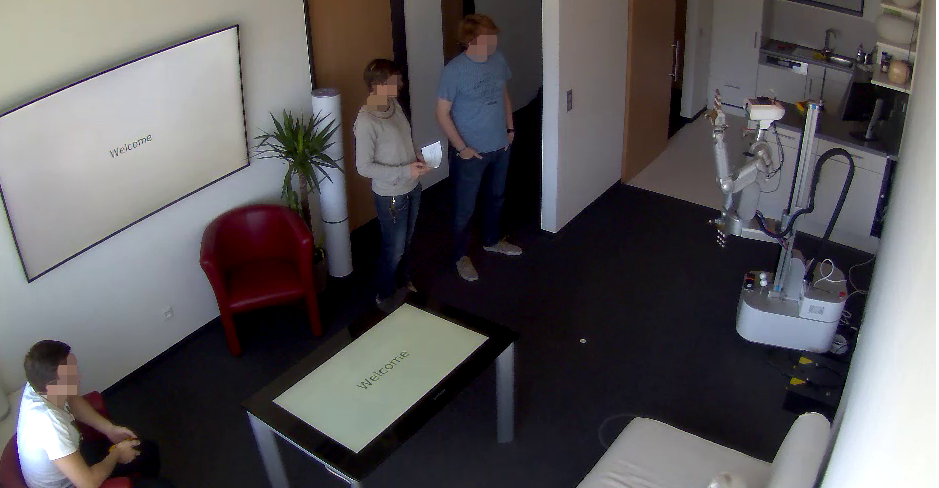
\includegraphics[trim={8cm 0 2cm 0},clip]{study-addressee-vp57}
          }
        };}
        \action<1->{\node[align=left, anchor=north, text width=.25\textwidth] (at) at (0, -.11\textwidth) {
        \textbf{RQ1 \scriptsize Addressing Behaviour}\\
          \vspace{5pt}
          \textcolor{mygreen}{\faCheckCircle} \Naive{} addressing\\
          \textcolor{mygreen}{\faCheckCircle} Attention\\
          \textcolor{mygreen}{\faCheckCircle} Speech
        };}
        \action<1->{\node (b) at (.25\textwidth+10,0)
        {
          \resizebox{.25\textwidth}{!}{%
            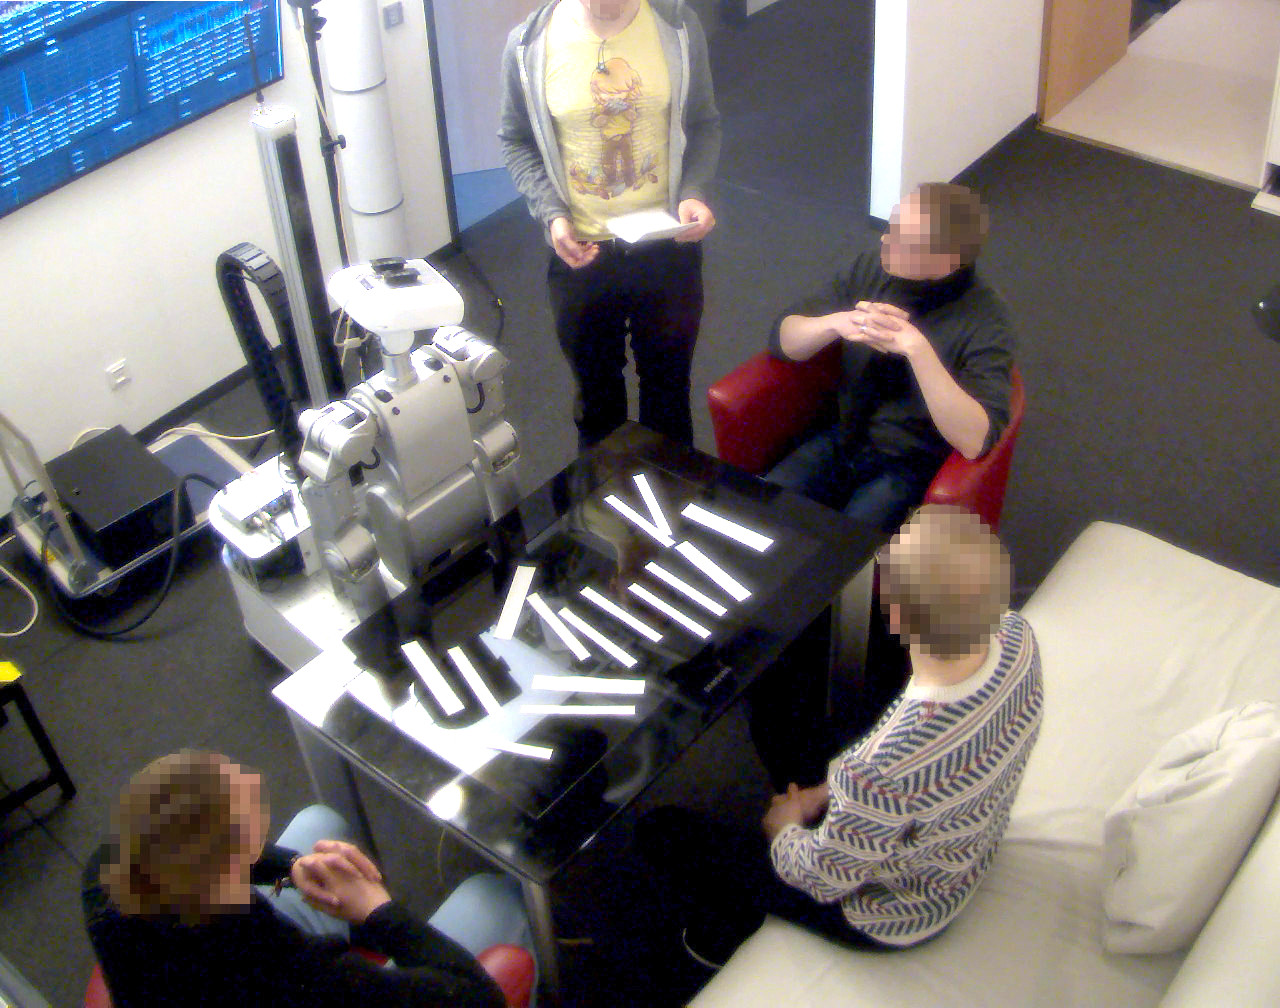
\includegraphics[trim={0 0 0 2cm},clip]{addressee-meka-intro}
          }
        };}
        \action<1->{\node[align=left, anchor=north, text width=.25\textwidth] (bt) at (.25\textwidth+10, -.11\textwidth) {
          \textbf{RQ2 \scriptsize Addressee Recognition}\\
          \vspace{5pt}
          \textcolor{mygreen}{\faCheckCircle} Mouth movements\\
          \textcolor{mygreen}{\faCheckCircle} Mutual gaze\\
          \textcolor{mygreen}{\faCheckCircle} Addressee\\
          };}
        \action<1->{\node (c) at (.5\textwidth+20,0)
        {
          \resizebox{.25\textwidth}{!}{%
            \input{generated/conversational_group_defence.pdf_tex}
          }
        };}
        \action<1->{\node[align=left, anchor=north, text width=.25\textwidth] (ct) at (.5\textwidth+20, -.11\textwidth) {
          \textbf{RQ3 \scriptsize Conversational Group}\\
          \vspace{5pt}
          \textcolor{mygreen}{\faCheckCircle} F-Formation\\
          \textcolor{mygreen}{\faCheckCircle} Gaze direction\\
          \textcolor{mygreen}{\faCheckCircle} Face detection\\
          };}
        \action<1->{\node (d) at (.75\textwidth+30,0)
        {
          \resizebox{.25\textwidth}{!}{%
            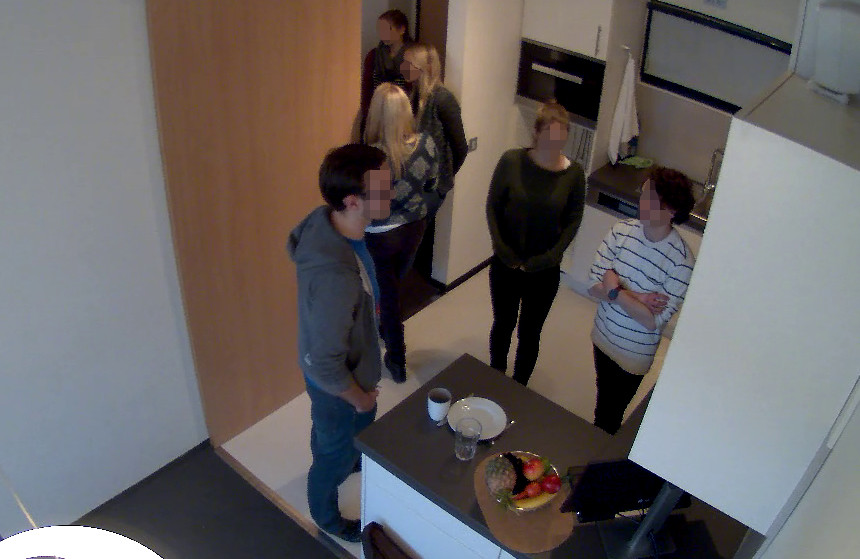
\includegraphics[trim={4.1cm 0 0 0},clip]{conversational_group}
          }
        };}
        \action<1->{\node[align=center, anchor=north, text width=.25\textwidth] (dt) at (.75\textwidth+30, -.11\textwidth) {
          \textbf{RQ4 \scriptsize Conversational Roles}\\
          \vspace{5pt}
          Repair \\ Interaction
        };}
        \action<1>{\filldraw [fill=bgcolorframe, draw=bgcolorframe, opacity=0.8, fill opacity=0.8] (380pt,-150pt) rectangle (270pt,40pt);}
        \action<2>{\filldraw [fill=bgcolorframe, draw=bgcolorframe, opacity=0.0, fill opacity=0.0] (380pt,-150pt) rectangle (270pt,40pt);}
\end{tikzpicture}
      }
  \pnote{25-14}
\end{frame}
